\documentclass[]{book}
\usepackage{lmodern}
\usepackage{amssymb,amsmath}
\usepackage{ifxetex,ifluatex}
\usepackage{fixltx2e} % provides \textsubscript
\ifnum 0\ifxetex 1\fi\ifluatex 1\fi=0 % if pdftex
  \usepackage[T1]{fontenc}
  \usepackage[utf8]{inputenc}
\else % if luatex or xelatex
  \ifxetex
    \usepackage{mathspec}
  \else
    \usepackage{fontspec}
  \fi
  \defaultfontfeatures{Ligatures=TeX,Scale=MatchLowercase}
\fi
% use upquote if available, for straight quotes in verbatim environments
\IfFileExists{upquote.sty}{\usepackage{upquote}}{}
% use microtype if available
\IfFileExists{microtype.sty}{%
\usepackage{microtype}
\UseMicrotypeSet[protrusion]{basicmath} % disable protrusion for tt fonts
}{}
\usepackage[margin=1in]{geometry}
\usepackage{hyperref}
\hypersetup{unicode=true,
            pdftitle={Beginning Computer Science with R},
            pdfauthor={Homer White},
            pdfborder={0 0 0},
            breaklinks=true}
\urlstyle{same}  % don't use monospace font for urls
\usepackage{natbib}
\bibliographystyle{apalike}
\usepackage{color}
\usepackage{fancyvrb}
\newcommand{\VerbBar}{|}
\newcommand{\VERB}{\Verb[commandchars=\\\{\}]}
\DefineVerbatimEnvironment{Highlighting}{Verbatim}{commandchars=\\\{\}}
% Add ',fontsize=\small' for more characters per line
\usepackage{framed}
\definecolor{shadecolor}{RGB}{248,248,248}
\newenvironment{Shaded}{\begin{snugshade}}{\end{snugshade}}
\newcommand{\KeywordTok}[1]{\textcolor[rgb]{0.13,0.29,0.53}{\textbf{{#1}}}}
\newcommand{\DataTypeTok}[1]{\textcolor[rgb]{0.13,0.29,0.53}{{#1}}}
\newcommand{\DecValTok}[1]{\textcolor[rgb]{0.00,0.00,0.81}{{#1}}}
\newcommand{\BaseNTok}[1]{\textcolor[rgb]{0.00,0.00,0.81}{{#1}}}
\newcommand{\FloatTok}[1]{\textcolor[rgb]{0.00,0.00,0.81}{{#1}}}
\newcommand{\ConstantTok}[1]{\textcolor[rgb]{0.00,0.00,0.00}{{#1}}}
\newcommand{\CharTok}[1]{\textcolor[rgb]{0.31,0.60,0.02}{{#1}}}
\newcommand{\SpecialCharTok}[1]{\textcolor[rgb]{0.00,0.00,0.00}{{#1}}}
\newcommand{\StringTok}[1]{\textcolor[rgb]{0.31,0.60,0.02}{{#1}}}
\newcommand{\VerbatimStringTok}[1]{\textcolor[rgb]{0.31,0.60,0.02}{{#1}}}
\newcommand{\SpecialStringTok}[1]{\textcolor[rgb]{0.31,0.60,0.02}{{#1}}}
\newcommand{\ImportTok}[1]{{#1}}
\newcommand{\CommentTok}[1]{\textcolor[rgb]{0.56,0.35,0.01}{\textit{{#1}}}}
\newcommand{\DocumentationTok}[1]{\textcolor[rgb]{0.56,0.35,0.01}{\textbf{\textit{{#1}}}}}
\newcommand{\AnnotationTok}[1]{\textcolor[rgb]{0.56,0.35,0.01}{\textbf{\textit{{#1}}}}}
\newcommand{\CommentVarTok}[1]{\textcolor[rgb]{0.56,0.35,0.01}{\textbf{\textit{{#1}}}}}
\newcommand{\OtherTok}[1]{\textcolor[rgb]{0.56,0.35,0.01}{{#1}}}
\newcommand{\FunctionTok}[1]{\textcolor[rgb]{0.00,0.00,0.00}{{#1}}}
\newcommand{\VariableTok}[1]{\textcolor[rgb]{0.00,0.00,0.00}{{#1}}}
\newcommand{\ControlFlowTok}[1]{\textcolor[rgb]{0.13,0.29,0.53}{\textbf{{#1}}}}
\newcommand{\OperatorTok}[1]{\textcolor[rgb]{0.81,0.36,0.00}{\textbf{{#1}}}}
\newcommand{\BuiltInTok}[1]{{#1}}
\newcommand{\ExtensionTok}[1]{{#1}}
\newcommand{\PreprocessorTok}[1]{\textcolor[rgb]{0.56,0.35,0.01}{\textit{{#1}}}}
\newcommand{\AttributeTok}[1]{\textcolor[rgb]{0.77,0.63,0.00}{{#1}}}
\newcommand{\RegionMarkerTok}[1]{{#1}}
\newcommand{\InformationTok}[1]{\textcolor[rgb]{0.56,0.35,0.01}{\textbf{\textit{{#1}}}}}
\newcommand{\WarningTok}[1]{\textcolor[rgb]{0.56,0.35,0.01}{\textbf{\textit{{#1}}}}}
\newcommand{\AlertTok}[1]{\textcolor[rgb]{0.94,0.16,0.16}{{#1}}}
\newcommand{\ErrorTok}[1]{\textcolor[rgb]{0.64,0.00,0.00}{\textbf{{#1}}}}
\newcommand{\NormalTok}[1]{{#1}}
\usepackage{longtable,booktabs}
\usepackage{graphicx,grffile}
\makeatletter
\def\maxwidth{\ifdim\Gin@nat@width>\linewidth\linewidth\else\Gin@nat@width\fi}
\def\maxheight{\ifdim\Gin@nat@height>\textheight\textheight\else\Gin@nat@height\fi}
\makeatother
% Scale images if necessary, so that they will not overflow the page
% margins by default, and it is still possible to overwrite the defaults
% using explicit options in \includegraphics[width, height, ...]{}
\setkeys{Gin}{width=\maxwidth,height=\maxheight,keepaspectratio}
\IfFileExists{parskip.sty}{%
\usepackage{parskip}
}{% else
\setlength{\parindent}{0pt}
\setlength{\parskip}{6pt plus 2pt minus 1pt}
}
\setlength{\emergencystretch}{3em}  % prevent overfull lines
\providecommand{\tightlist}{%
  \setlength{\itemsep}{0pt}\setlength{\parskip}{0pt}}
\setcounter{secnumdepth}{5}
% Redefines (sub)paragraphs to behave more like sections
\ifx\paragraph\undefined\else
\let\oldparagraph\paragraph
\renewcommand{\paragraph}[1]{\oldparagraph{#1}\mbox{}}
\fi
\ifx\subparagraph\undefined\else
\let\oldsubparagraph\subparagraph
\renewcommand{\subparagraph}[1]{\oldsubparagraph{#1}\mbox{}}
\fi

%%% Use protect on footnotes to avoid problems with footnotes in titles
\let\rmarkdownfootnote\footnote%
\def\footnote{\protect\rmarkdownfootnote}

%%% Change title format to be more compact
\usepackage{titling}

% Create subtitle command for use in maketitle
\newcommand{\subtitle}[1]{
  \posttitle{
    \begin{center}\large#1\end{center}
    }
}

\setlength{\droptitle}{-2em}
  \title{Beginning Computer Science with R}
  \pretitle{\vspace{\droptitle}\centering\huge}
  \posttitle{\par}
  \author{Homer White}
  \preauthor{\centering\large\emph}
  \postauthor{\par}
  \predate{\centering\large\emph}
  \postdate{\par}
  \date{2017-07-17}

\usepackage{booktabs}
\usepackage{longtable}
\usepackage[bf,singlelinecheck=off]{caption}
\usepackage[utf8]{inputenc}

\usepackage{framed,color}
\definecolor{shadecolor}{RGB}{248,248,248}

\renewcommand{\textfraction}{0.05}
\renewcommand{\topfraction}{0.8}
\renewcommand{\bottomfraction}{0.8}
\renewcommand{\floatpagefraction}{0.75}

%\renewenvironment{quote}{\begin{VF}}{\end{VF}}
\let\oldhref\href
\renewcommand{\href}[2]{#2\footnote{\url{#1}}}

\renewcommand{\textfraction}{0.05}
\renewcommand{\topfraction}{0.8}
\renewcommand{\bottomfraction}{0.8}
\renewcommand{\floatpagefraction}{0.75}

%\renewenvironment{quote}{\begin{VF}}{\end{VF}}
\let\oldhref\href
\renewcommand{\href}[2]{#2\footnote{\url{#1}}}

\ifxetex
  \usepackage{letltxmacro}
  \setlength{\XeTeXLinkMargin}{1pt}
  \LetLtxMacro\SavedIncludeGraphics\includegraphics
  \def\includegraphics#1#{% #1 catches optional stuff (star/opt. arg.)
    \IncludeGraphicsAux{#1}%
  }%
  \newcommand*{\IncludeGraphicsAux}[2]{%
    \XeTeXLinkBox{%
      \SavedIncludeGraphics#1{#2}%
    }%
  }%
\fi

\makeatletter
\newenvironment{kframe}{%
\medskip{}
\setlength{\fboxsep}{.8em}
 \def\at@end@of@kframe{}%
 \ifinner\ifhmode%
  \def\at@end@of@kframe{\end{minipage}}%
  \begin{minipage}{\columnwidth}%
 \fi\fi%
 \def\FrameCommand##1{\hskip\@totalleftmargin \hskip-\fboxsep
 \colorbox{shadecolor}{##1}\hskip-\fboxsep
     % There is no \\@totalrightmargin, so:
     \hskip-\linewidth \hskip-\@totalleftmargin \hskip\columnwidth}%
 \MakeFramed {\advance\hsize-\width
   \@totalleftmargin\z@ \linewidth\hsize
   \@setminipage}}%
 {\par\unskip\endMakeFramed%
 \at@end@of@kframe}
\makeatother

\renewenvironment{Shaded}{\begin{kframe}}{\end{kframe}}

\newenvironment{rmdblock}[1]
  {
  \begin{itemize}
  \renewcommand{\labelitemi}{
    \raisebox{-.7\height}[0pt][0pt]{
      {\setkeys{Gin}{width=3em,keepaspectratio}\includegraphics{images/#1}}
    }
  }
  \setlength{\fboxsep}{1em}
  \begin{kframe}
  \item
  }
  {
  \end{kframe}
  \end{itemize}
}

\newenvironment{leadquote}
  {
  \begin{kframe}
  }
  {
  \end{kframe}
}


\newenvironment{rmdnote}
  {\begin{rmdblock}{note}}
  {\end{rmdblock}}
\newenvironment{rmdcaution}
  {\begin{rmdblock}{caution}}
  {\end{rmdblock}}
\newenvironment{rmdimportant}
  {\begin{rmdblock}{important}}
  {\end{rmdblock}}
\newenvironment{rmdtip}
  {\begin{rmdblock}{tip}}
  {\end{rmdblock}}
\newenvironment{rmdwarning}
  {\begin{rmdblock}{warning}}
  {\end{rmdblock}}

\usepackage{makeidx}
\makeindex

\urlstyle{tt}

\usepackage{amsthm}
\makeatletter
\def\thm@space@setup{%
  \thm@preskip=8pt plus 2pt minus 4pt
  \thm@postskip=\thm@preskip
}
\makeatother

\usepackage{amsthm}
\newtheorem{theorem}{Theorem}[chapter]
\newtheorem{lemma}{Lemma}[chapter]
\theoremstyle{definition}
\newtheorem{definition}{Definition}[chapter]
\newtheorem{corollary}{Corollary}[chapter]
\newtheorem{proposition}{Proposition}[chapter]
\theoremstyle{definition}
\newtheorem{example}{Example}[chapter]
\theoremstyle{remark}
\newtheorem*{remark}{Remark}
\let\BeginKnitrBlock\begin \let\EndKnitrBlock\end
\begin{document}
\maketitle

{
\setcounter{tocdepth}{1}
\tableofcontents
}
\chapter*{Preface}\label{preface}
\addcontentsline{toc}{chapter}{Preface}

Welcome to \emph{Beginning Computer Science with R}! These notes will be
your primary source for CSC 115: Computer Science I, offered at
Georgetown College. They will also carry you part of the way through CSC
215. A supplementary text, \emph{Hands-On Programming with R} by Garrett
Grolemund \citep{Grolemund2014}, will be used in CSC 115 so you should
make sure that you have a copy.

For the first semester you won't need a computer of your own: you can do
all of your work on the R Studio Server, which you will access with your
College network username and password. Eventually, though, you will need
to learn how to install and maintain professional software development
tools on your own machine, so at some point early on in CSC 215 you will
install R, R Studio and various other tools on a laptop of your own.
Then you will bring the laptop to class for your daily work.

These Notes are available not only on the web but also as a PDF document
that can be downloaded from the website (click the PDF icon, found among
the icons at the top of the page). The PDF is useful when you are
working offline, and it also has an index.

Instructional videos on selected topics will be published from time to
time on this YouTube Channel:
\url{https://www.youtube.com/user/GCstats}, in the CSC playlist.

These notes are about the R programming language as such, so although in
the class we will work within the R Studio Integrated Deveopment
Environment right from the start, R Studio is not directly covered here.
Eventually we will begin to write documents in R Markdown, which is also
not treated in these Notes. For a resource on these topics in written
form that will supplement class instructon and the videos on our YouTube
Channel, you might want to consult the excellent little book
\href{https://bookdown.org/chesterismay/rbasics/}{\emph{Getting used to
R, RStudio, and R Markdown}} \citep{Ismay2016}.

\section{The Why of these Notes: Remarks for
Colleagues}\label{the-why-of-these-notes-remarks-for-colleagues}

There is a plethora of books on R, covering pretty much every domain of
application of the language, from ecology to spatial statistics to
machine learning and data science. There are even some books---among the
very finest of R-books, in my view---on R as a a programming language.
Why then, write yet another book?

It all has to do with my particular situation. As Fate and the vagueries
of small-college staffing would have it, I find myself preparing to
teach the minor in Computer Science at the liberal arts College where
for many years I had previously taught mathematics and statistics. As I
considered how to redesign a minor lean enough to be staffed by one
not-quite-full-time person (I still handle some mathematics) and at the
same offer something of absorbing interest to a reasonable number of
undergraduates, I realized that it could not simply be a truncated
version of a major: a year of programming in a strongly-typed, compiled,
large-scale programming language such as C++ or Java, followed by
algorithms, data structures, compilers and perhaps a bit of theory. For
one thing, I shy away from large-scale languages: I tend to want my
results fast and I want to build something interesting as soon as
possible, and for the most part beginning students feel the same way.
About the only thing a minor as a curtailed major would prepare them for
is, well, \emph{completion} of the major---which unfortunately we do not
have. For another thing, my background simply isn't in Computer Science.
I am by training a mathematician with a specialty in ergodic theory,
which could be considered an extreme generalization of probability
theory. Computer programming, with its fetish for the careful
organization of information and its stress on practices to manage
complexity, simply isn't in my theoretical blood.

On the other hand in my years of teaching and practicing statistics I
have gotten to be a half-good programmer by recognizing, through hard
experience, the value of learning to program well from the ground up. I
have become increasingly fascinated by the computational aspects of
statistics and by the entire computer-based workflow of data
analysis---from data collection and data munging to analysis and
reporting---and by the paradigm of reproducible research that can be
incorporated into nearly every stage of that workflow. With the tendency
of data analysis to move toward the web I'm also seeing the utility of
being aware of web design issues as a data analyst, and, as a web
designer and developer, of being cognizant of trends in internet-based
data collection and data reporting.

Accordingly the minor will have a dual focus: data analysis and web
design, with a bit of back-end web development thrown in to unify the
two domains. Students will undertake a serious study of two major
scripting languages: R for data analysis and JavaScript for web
programming, both from a fairly systematic programming point of view,
with due attention to procedural, object-oriented and (to a lesser
extent) functional programming paradigms.

The question is: which language to use in the freshman year? Some
institutions are moving toward JavaScript: in fact Stanford University
will pilot JavaScript in several sections of its introductory CS course
in the Fall of 2017. There are certainly considerations in favor of a
JavaScript-first approach: it's a popular language with Node available
as an interactive run-time environment and the browser as a environment
in which exciting applications can be built quickly. And whereas R is
less widely-used and is still considered a domain-specific language,
JavaScript can rightly be said to have made the leap into the ranks of
general-purpose programming languages. R also has the reputation of
being a prickly language with a somewhat inconsistent syntax and with
documentation that is ``expert-friendly'' at best.

On the other hand R is designed for one-line interactivity at the
console, so it's possible for a beginner to get simple programs working
quickly. The R-ecosystem has also become a lot more user-friendly in
recent years. The
\href{https://www.rstudio.com/products/rstudio/}{RStudio} IDE is
comparable to top-flight integrated development environments for many
other major languages and yet is still relatively lightweight and
accessible to beginners. The Server version of R Studio is especially
useful for new programmers, as it saves them from having to deal with
installation and other IT issues on their own machines, permitting them
to focus on coding. It's also easy, in a server setting, to make class
materials available and to collect and return assignments. R Markdown is
fine platform for producing course notes (this book is written in R
Markdown with the excellent \textbf{bookdown} package
\citep{R-bookdown}) and slides as well. Students, too, can use R
Markdown to both write and discuss their programs in a single document.
The \textbf{blogdown} package \citep{R-blogdown} permits students to
begin writing for the public about technical programming issues---or
about anything at all, really, as more than a few of them are taking
majors in the Humanities---thus building up an professional resume of
online work. Finally, the \textbf{shiny} package \citep{R-shiny} permits
students to build simple interactive web apps for data analysis that can
be used by non-coders. Both \textbf{blogdown} and \textbf{shiny} prompt
students to consider early on---even in the first year, if the pacing is
right---concepts of web design, the other primary focus of the minor.

Hence the choice was made to teach a first-year computer science course,
to beginning programmers, with R. As I pointed out earlier, there do
exist some excellent books on R as a programming language that do not
presume previous experience with R. One example is Norman Matloff's
\emph{The Art of R Programming} \citep{Matloff2011}. Matloff, however,
presumes that the reader either has prior programming experience in some
other language or else possesses sufficient computational maturity,
acquired perhaps through extensive prior training in the mathematical
sciences. Another great text is Garrett Grolemund's \emph{Hands-on
Programming with R} \citep{Grolemund2014}. Grolemund's book is lively
and to-the-point and starts off with excellent motivating examples.
Grolemund is also a master explainer, and he has put considerable effort
into visual representation of programming concepts such as element-wise
operations on vectors and the enclosure-relationships between
environments; for that reason his text is being used as a supplementary
textbook for this course. On the other hand, even though he doesn't
assume that the reader has prior coding experience, Grolemund does
assume some prior background in data analysis and a strong motivation,
on the reader's part, to persevere with nontrivial R-programming issues
such as lexical scoping in the hopes of eventual payoffs in programming
for data science. In short, Grolemund also assumes more computational
maturity than will be usually be found among beginning programmers at
many small liberal arts colleges.

Hence the niche for the notes (or perhaps text-under-development)
offered here. I aim to be a bit more copious and slow-paced than
Grolemund and a bit less sophisticated than Matloff. These notes will
also contain a more extensive set of problems, ranging in difficulty
from practice exercises to fairly extended projects that students might
write up in R Markdown documents.

Experienced programmers and R enthusiasts will be struck by the absence
of certain topics. Programmers will observe that there is no real
attention to algorithms (sorting is just \texttt{sort()} or
\texttt{order()}), and although functions receive lots of attention
there is no mention of recursion. In future editions I might cover
recursion, as I believe that it is wonderful for the development of
thinking skills, but it's not likely that a web developer or data
analyst would have the need to write a recursive function. Time spent on
recursion and on various efficient algorithms for sorting and searching
may be better spent, in my view, on extended programming projects, Shiny
apps and blogging, and introductions to tools of the programmer's trade
such as version control and GitHub. I hope by the end of the first year
to have made time for all of these ``extra'' topics. R-specific tools
such as \textbf{dplyr} for data manipulation, the various packages for
web scraping and database interface, as well as packages for machine
learning, are considered in later courses in the minor that are more
specifically concerned with data analysis.

Two of the most fundamental topics in any comprehensive discussion of
the R language---lexical scoping and computing on the language---are
absent from this book. Lexical scoping and its implications are
mentioned only in a brief footnote. Partly this is due the fact that
most of the elementary applications of lexical scoping mentioned in the
literature are related to scientific computing, which won't be a concern
for most of my students. Certainly lexical scoping is important for
understanding how R-packages work, but elementary students don't author
packages. As for computing on the language it is true that users are
affected by it all the time (e.g., whenever they use functions with a
formula interface), but generally one need not perform any computation
on the language until one begins writing formula-interface functions for
the benefit of casual R-users.

On the other hand I have made some effort to explore programming
paradigms other than procedural programming, perhaps in a bit more depth
than in other elementary texts that teach with a scripting language.
There is a chapter on functional programming that, although it
admittedly does not get far into the functional paradigm, at least does
treat extensively of R's support for higher-order functions. A chapter
on object-oriented programming covers not only the generic-function OO
that has been with R from the start but also an implementation of
message-passing OO (Winston Chang's \textbf{R6} package \citep{R-R6}).
My hope is that these topics will not only sharpen my students'
R-programming skills but also prepare them for encounters with the
OO-methods and higher-order functions that are ubiquitous in JavaScript.
Finally, there is a pretty serious chapter on regular expressions,
because:

\begin{itemize}
\tightlist
\item
  they are useful in data analysis;
\item
  I have not found a treatment of regular expressions in R that a person
  without significant prior exposure to them in other languages has a
  prayer of following;
\item
  and because if you master regular expressions then you feel like a
  wizard.
\end{itemize}

As for the numerous Wizard of Oz-themed examples, I can offer no defense
other than haste. Perhaps a future version will be built around
something more suitable---the Harry Potter series, say.

\section{History of R}\label{history-of-r}

The story of R begins at
\href{https://en.wikipedia.org/wiki/Bell_Labs}{Bell Labs} in 1975, with
the development, by John Chambers and several other colleagues, of the S
language for statistical computing. The language became well-known among
statisticians and data analysts, especially in the academic community.

In the early 1990's Ross Ihaka of the University of Auckland in New
Zealand was making a study of the Scheme language as described in the
classic MIT textbook \emph{Structure and Interpretation of Computer
Programs} \citep{AbelsonSussman}, and was impressed with the
possibilities of the language for data analysis applications. Desiring
to build a free analysis tool for his graduate students, Ihaka teamed up
with his Auckland colleague Robert Gentleman and the two gradually
developed a language with an external syntax similar to S but with an
underlying engine based heavily upon Scheme. Because of the similarity
with the better-known S---or, by some account, because of the initial
letter in the first names of both men---they named their new language
``R''.

Initially the two men believed that their work on the new language was
scarcely more than ``playing games'' and that it would not be used
outside of the University of Auckland. Eventually, though, the two
placed a small announcement of their project on the email list
\emph{s-news} and began to draw the interest of other statisticians,
including Martin Machler of the Swiss Federal Institute of Technology in
Zurich, Switzerland. Machler saw great potential for R, and in 1995
persuaded Ihaka and Gentleman to release it as ``free software'' under a
\href{https://www.gnu.org/licenses/gpl-faq.html\#WhatDoesGPLStandFor}{GNU
Public License}. The decision to make R free stimulated further interest
in the language and encouraged many experts in statistical computation
to become involved in its further development.

The first official public release of R (version 1.0.0) occurred on
February 29, 2000. Since that time R has grown in popularity at an
increasing rate, to the point where it is by now one of the world's most
widely-used domain-specific computer languages, ranking among the top
dozen computer languages overall.

Many people have contributed to the development of R. As of the
composition of this History, the Comprehensive R Archive Network (CRAN)
now hosts 10,633 contributed packages, each of which aims to extend the
capabilities of R in a specific way. R is usually the platform in which
new statistical techniques are first implemented by the researchers who
develop them. It is widely used in the sciences, business and finance.

\section{Acknowledgements}\label{acknowledgements}

I am greatly indebted to:

\emph{Norman Matloff} and \emph{Hadley Wickham} for their excellent
foundational books (\citep{Matloff2011}, \citep{Wickham2014}) on the R
language. \emph{Garrett Grolemund}, for his informal but precise
expository style, as exemplified in numerous R Studio webinars and in
\citep{Grolemund2014}.

\emph{Allen Downey}, for \emph{Think Python} \citep{Downey2015}. This
book formed my ideas about ordering and selection of topics for computer
science at an elementary level, and helped me think about teaching
computer science in a way that was as independent as possible from the
specific language of instruction.

\emph{Everyone} at R Studio, including Hadley, \emph{Yihui Xie} for R
Markdown and the family of R Markdown-related packages, \emph{Joe Cheng}
for conceiving and pioneering \textbf{shiny}, \emph{Winston Chang} for
\textbf{shiny} and \textbf{R6}, and of course \emph{JJ Allaire} for
developing the IDE and calling together the remarkable constellation of
developers and evangelists who have contributed so much to the R
community and ecosystem.

\emph{Danny Kaplan}, \emph{Nick Horton} and \emph{Randall Pruim} for
pioneering the Mosaic Project that has enabled so many faculty to teach
undergraduate statistics with R. I am especially indebted to Danny for
curricular inspiration and to Randall for R-programming advice in the
incipient stages of my journey as an R-developer. Nick has been a great
encourager of everyone associated with the Mosaic community.

My former colleague \emph{Rebekah Robinson} who, upon learning of Mosaic
and R Markdown, insisted that at Georgetown we should figure out how to
teach elementary statistics with R.

My colleagues \emph{William Harris} and \emph{Christine Leverenz}, who
learned to teach in the R way.

My students, especially \emph{Woody Burchett}, \emph{Luke Garnett},
\emph{Shawn Marcom}, \emph{Jacob Townsend} and \emph{Andrew Giles}, for
work with me on various R-related research projects. Luke has gone on to
become a valued colleague at Georgetown.

\emph{Georgetown College}, for granting me the sabbatical time in Spring
2017 to work on these Notes, and on other programming topics
prerequisite to teaching Computer Science.

My wife \emph{Mary Lou} and daughters \emph{Clare}, \emph{Catherine} and
\emph{Agnes}, for patience and support. By now they have heard quite
enough about programming.

\section{Miscellaneous Information}\label{miscellaneous-information}

\subsection{Typographical Conventions}\label{typographical-conventions}

Computer code, whether within a line of text or as displayed text,
appears like this: \texttt{code\ snippet}.

Identifiers are represented as is (e.g., \texttt{variableName},
if\texttt{,}else\texttt{,}while\texttt{,\ etc.)\ except\ for\ the\ names\ of\ functions,\ whihc\ are\ followed\ by\ a\ pair\ of\ parentheses\ in\ order\ to\ stress\ their\ status\ as\ functions.\ \ Thus\ we\ write}length()\texttt{for\ the}length`-function.

Displayed text representing output to the console appears with double
hash-tags at the beginning of each line, thus:

\begin{verbatim}
## R is free software and comes with ABSOLUTELY NO WARRANTY.
## You are welcome to redistribute it under certain conditions.
## Type 'license()' or 'licence()' for distribution details.
\end{verbatim}

The hashtags themsevles are not present in the output itself.

Names of R-package are in boldface, thus: package \textbf{devtools}.

Terms are italicized when they are first introduced, e.g.: ``R follows a
set of internal rules to \emph{coerce} some of the values to a new type
in such a way that all resulting values are of the same type.''
Italicization can also indicate emphasis.

\subsection{License}\label{license}

These Notes are licensed under the Creative Commons
Attribution-ShareAlike 4.0 International Public License:

\begin{quote}
\url{https://creativecommons.org/licenses/by-sa/4.0/legalcode}.
\end{quote}

\chapter{Our First Computer Programs}\label{idea}

\begin{figure}[!h]

{\centering 
\includegraphics[width=0.7\linewidth]{images/yellow_brick_road} 

}

\caption{The Yellow Brick Road, by Jorge Cruz.  [clipartfest.com](https://clipartfest.com/).}\label{fig:beginning-journey}
\end{figure}

\newpage

\section{Hello, World!}\label{hello-world}

Let's write our very first computer program. \index{computer program}
Type the following code into the console and press \textbf{Enter}:

\begin{Shaded}
\begin{Highlighting}[]
\KeywordTok{cat}\NormalTok{(}\StringTok{"Hello, World!"}\NormalTok{)}
\end{Highlighting}
\end{Shaded}

In the console you should see the following output:

\begin{verbatim}
## Hello, World!
\end{verbatim}

That's it---you just wrote a \emph{computer program}. A computer program
is simply a sequence of instructions tha perform a specific task when
they are \emph{executed} (carried out) by the computer. In the above
example, there was only one instruction in the sequence: it was the
command to reproduce the \emph{string} \index{string} ``Hello, World''
in the console exactly as it is. The name of that command is
\texttt{cat()}.

Let's try another small program.

Type the following code into the console and press \textbf{Enter}:

\begin{Shaded}
\begin{Highlighting}[]
\KeywordTok{cat}\NormalTok{(}\DecValTok{2+2}\NormalTok{)}
\end{Highlighting}
\end{Shaded}

In the console you should see the following output:

\begin{verbatim}
## 4
\end{verbatim}

We have been using the \texttt{cat()}
\index{R-functions!cat()@\texttt{cat()}}function so far. Actually you
can can get output without it. For example, suppose you type:

\begin{Shaded}
\begin{Highlighting}[]
\StringTok{"Hello, World!"}
\end{Highlighting}
\end{Shaded}

Then in the console you see:

\begin{verbatim}
## [1] "Hello World"
\end{verbatim}

There are quote-marks around the text: that's not so pretty, but we
still get the basic output.

Similarly, you can try:

\begin{Shaded}
\begin{Highlighting}[]
\DecValTok{2+2}
\end{Highlighting}
\end{Shaded}

\begin{verbatim}
## [1] 4
\end{verbatim}

Notice that when we don't use \texttt{cat()} the output begins with a
strange \texttt{{[}1{]}}. In the next chapter we'll learn why this
happens; for now, just ignore it.

\section{A Quick Tour}\label{idea-tour}

We now embark on a tour of some of R's basic capabilities. In later
chapters we will examine in detail the programming concepts that
underlie the features we explore now.

\subsection{Basic Arithmetic}\label{idea-arithmetic}

R can be treated like a calculator. You can:

\begin{itemize}
\tightlist
\item
  add numbers (\texttt{+})
\item
  subtract numbers (\texttt{-})
\item
  multiply numbers (\texttt{*})
\item
  divide numbers (\texttt{/})
\item
  raise a number to a power (\texttt{\^{}})
\end{itemize}

Just as on a graphing calculator, parentheses can be used to clarify the
order of operations.

Here are some examples:

To get \(\frac{27-10}{3}\), use:

\begin{Shaded}
\begin{Highlighting}[]
\NormalTok{(}\DecValTok{27-3}\NormalTok{)/}\DecValTok{10}
\end{Highlighting}
\end{Shaded}

\begin{verbatim}
## [1] 2.4
\end{verbatim}

To get \(3^2 + 4^2\) try:

\begin{Shaded}
\begin{Highlighting}[]
\DecValTok{3}\NormalTok{^}\DecValTok{2+4}\NormalTok{^}\DecValTok{2}
\end{Highlighting}
\end{Shaded}

\begin{verbatim}
## [1] 25
\end{verbatim}

Sometimes you'll want to take roots. As with a calculator, you can
accomplish this by raising your number to a fractional power. So if you
want \(\sqrt[3]{64}\) then you could try:

\begin{Shaded}
\begin{Highlighting}[]
\DecValTok{64}\NormalTok{^\{}\DecValTok{1}\NormalTok{/}\DecValTok{3}\NormalTok{\}}
\end{Highlighting}
\end{Shaded}

\begin{verbatim}
## [1] 4
\end{verbatim}

If you would like square roots then you can either raise your number to
the \(1/2\)-power or you could use R's special square-root function:

\begin{Shaded}
\begin{Highlighting}[]
\KeywordTok{sqrt}\NormalTok{(}\DecValTok{64}\NormalTok{)}
\end{Highlighting}
\end{Shaded}

\begin{verbatim}
## [1] 8
\end{verbatim}

One way or another, you can evaluate quite complex mathematical
expressions. For example, to get \(\sqrt{3^2 + 4^2}\) simply type:

\begin{Shaded}
\begin{Highlighting}[]
\KeywordTok{sqrt}\NormalTok{(}\DecValTok{3}\NormalTok{^}\DecValTok{2+4}\NormalTok{^}\DecValTok{2}\NormalTok{)}
\end{Highlighting}
\end{Shaded}

\begin{verbatim}
## [1] 5
\end{verbatim}

\subsection{Read-Evaluate-Print-Loop}\label{read-evaluate-print-loop}

So far you have been using R in what computer scientists call
\emph{interactive mode}. This means that you type something in at the
console; R immedidately reads what you type and evaluates it, and prints
the resulting value to the console for you to see. Then you type
something else, and so on. This back-and-forth process is often called
the \emph{Read-Evaluate-Print-Loop}, or REPL \index{REPL} for short. R
is one of several computer languages that make it easy for you to see
the results of its computations in the console. That's because it was
originally designed for use by statisticians and data analysts, who
often want to run a small procedure, check on the results and then try a
new or related procedure and check on the results \ldots{} until their
analysis is complete. From our point of view as beginning programmers,
though, the REPL makes it easy to see what R is doing and to get
immediate feedback on the very simple programs that we are now writing.

\subsection{Variables}\label{idea-variables}

Quite often you will want to use the same value several different times.
You can so this by creating a \emph{variable} \index{variables} with the
\emph{assignment operator} \texttt{\textless{}-}.
\index{R-operators!<- (assignment)}

\begin{Shaded}
\begin{Highlighting}[]
\NormalTok{a <-}\StringTok{ }\DecValTok{10}
\end{Highlighting}
\end{Shaded}

The previous statement puts the value 10 in the computer's memory and
causes the name \texttt{a} to refer to it. If you ask R to show you
\texttt{a}, you'll get that value:

\begin{Shaded}
\begin{Highlighting}[]
\NormalTok{a}
\end{Highlighting}
\end{Shaded}

\begin{verbatim}
## [1] 10
\end{verbatim}

Now you can use \texttt{a} as much as you like:

\begin{Shaded}
\begin{Highlighting}[]
\NormalTok{a +}\StringTok{ }\DecValTok{23}
\end{Highlighting}
\end{Shaded}

\begin{verbatim}
## [1] 33
\end{verbatim}

\begin{Shaded}
\begin{Highlighting}[]
\KeywordTok{sqrt}\NormalTok{(a)}
\end{Highlighting}
\end{Shaded}

\begin{verbatim}
## [1] 3.162278
\end{verbatim}

Later on if you want to make \texttt{a} point to a different value, you
can do so:

\begin{Shaded}
\begin{Highlighting}[]
\NormalTok{a <-}\StringTok{ }\DecValTok{4}
\NormalTok{a +}\StringTok{ }\DecValTok{23}
\end{Highlighting}
\end{Shaded}

\begin{verbatim}
## [1] 27
\end{verbatim}

You can choose variable-names that are descriptive. Let's write some
code to introduce creatures of various types. A creatuee should give his
or her name, say what type of creature he or she is, and name a favorite
food.

\begin{Shaded}
\begin{Highlighting}[]
\NormalTok{creatureType <-}\StringTok{"Munchkin"}
\NormalTok{creatureName <-}\StringTok{ "Boq"}
\NormalTok{creatureFood <-}\StringTok{ "corn"}
\end{Highlighting}
\end{Shaded}

Next, let's combine these items into a greeting:

\begin{Shaded}
\begin{Highlighting}[]
\KeywordTok{paste}\NormalTok{(}\StringTok{"Hello, I am a "}\NormalTok{,}
      \NormalTok{creatureType,}
      \StringTok{". My name is "}\NormalTok{,}
      \NormalTok{creatureName,}
      \StringTok{".  I like to eat "}\NormalTok{,}
      \NormalTok{creatureFood,}
      \StringTok{"."}\NormalTok{,}
      \DataTypeTok{sep =} \StringTok{""}\NormalTok{)}
\end{Highlighting}
\end{Shaded}

\begin{verbatim}
## [1] "Hello, I am a Munchkin. My name is Boq.  I like to eat corn."
\end{verbatim}

We see that \texttt{paste()}
\index{R-functions!paste()@\texttt{paste()}}function puts strings
together. The \texttt{sep\ =\ ""} argument at the end specifies that no
space is to be inserted between the strings when they combined.

Another thing we notice in the previous code is that R can ignore white
space: we were able to separate parts of the command to different lines.
This helps prevent our lines from being too long, and allows us to
arrange the code so that it's easy to read.

Spaces do matter inside a string, though:

\begin{Shaded}
\begin{Highlighting}[]
\NormalTok{kalidah <-}\StringTok{ "Teddy"}
\NormalTok{kalidah}
\end{Highlighting}
\end{Shaded}

\begin{verbatim}
## [1] "Teddy"
\end{verbatim}

\begin{Shaded}
\begin{Highlighting}[]
\NormalTok{kalidah2 <-}\StringTok{ "Ted  dy"}
\NormalTok{kalidah2}
\end{Highlighting}
\end{Shaded}

\begin{verbatim}
## [1] "Ted  dy"
\end{verbatim}

You must also be careful not to insert spaces within the name of any
object:

\begin{Shaded}
\begin{Highlighting}[]
\NormalTok{kali dah2}
\end{Highlighting}
\end{Shaded}

\begin{Shaded}
\begin{Highlighting}[]
\NormalTok{## Error: unexpected symbol in "kali dah2"}
\end{Highlighting}
\end{Shaded}

R got confused by the unexpected space: it knows about the name
\texttt{kalidah2}, but \texttt{kali\ dah2} means nothing.

Getting back to the Oz-creatures: it would be nice if a creatures's
greeting could be split over several lines. This is possible if you use
the special string ``\textbackslash{}n'', which produces a newline. Just
incorporate it into your message, as follows:

\begin{Shaded}
\begin{Highlighting}[]
\KeywordTok{paste}\NormalTok{(}\StringTok{"Hello, I am a "}\NormalTok{,}
      \NormalTok{creatureType,}
      \StringTok{".}\CharTok{\textbackslash{}n}\StringTok{My name is "}\NormalTok{,}
      \NormalTok{creatureName,}
      \StringTok{".}\CharTok{\textbackslash{}n}\StringTok{I like to eat "}\NormalTok{,}
      \NormalTok{creatureFood,}
      \StringTok{"."}\NormalTok{,}
      \DataTypeTok{sep =} \StringTok{""}\NormalTok{)}
\end{Highlighting}
\end{Shaded}

\begin{verbatim}
## [1] "Hello, I am a Munchkin.\nMy name is Boq.\nI like to eat corn."
\end{verbatim}

That doesn't look like an improvement at all! But what if we were to
\texttt{cat()} it?

\begin{Shaded}
\begin{Highlighting}[]
\NormalTok{message <-}\StringTok{ }\KeywordTok{paste}\NormalTok{(}\StringTok{"Hello, I am a "}\NormalTok{,}
                 \NormalTok{creatureType,}
                 \StringTok{".}\CharTok{\textbackslash{}n}\StringTok{My name is "}\NormalTok{,}
                 \NormalTok{creatureName,}
                 \StringTok{".}\CharTok{\textbackslash{}n}\StringTok{I like to eat "}\NormalTok{,}
                 \NormalTok{creatureFood,}
                 \StringTok{"."}\NormalTok{,}
                 \DataTypeTok{sep =} \StringTok{""}\NormalTok{)}
\KeywordTok{cat}\NormalTok{(message)}
\end{Highlighting}
\end{Shaded}

\begin{verbatim}
## Hello, I am a Munchkin.
## My name is Boq.
## I like to eat corn.
\end{verbatim}

That's much nicer.

That last example showed that you can use variables together with
functions to create new variables. Here is another example:

\begin{Shaded}
\begin{Highlighting}[]
\NormalTok{a <-}\StringTok{ }\DecValTok{10}
\NormalTok{b <-}\StringTok{ }\DecValTok{27}
\NormalTok{mySum <-}\StringTok{ }\NormalTok{a +}\StringTok{ }\NormalTok{b}
\NormalTok{mySum}
\end{Highlighting}
\end{Shaded}

\begin{verbatim}
## [1] 37
\end{verbatim}

\subsection{Functions}\label{idea-functions}

Let's say that we want to introduce George the Quadling. We might try:

\begin{Shaded}
\begin{Highlighting}[]
\NormalTok{creatureName <-}\StringTok{ "George"}
\NormalTok{creatureType <-}\StringTok{ "Quadling"}
\NormalTok{creatureFood <-}\StringTok{ "cookies"}
\KeywordTok{cat}\NormalTok{(message)}
\end{Highlighting}
\end{Shaded}

\begin{verbatim}
## Hello, I am a Munchkin.
## My name is Boq.
## I like to eat corn.
\end{verbatim}

Hmm, that didn't go so well: we got Boq instead. The problem is that the
variable\texttt{message} was created using the original values of
\texttt{creatureName}, \texttt{creatureType} and \texttt{creatureFood},
not the new values that we are interested in. To do it right we should
have re-made \texttt{message}, as follows:

\begin{Shaded}
\begin{Highlighting}[]
\NormalTok{creatureName <-}\StringTok{ "George"}
\NormalTok{creatureType <-}\StringTok{ "Quadling"}
\NormalTok{creatureFood <-}\StringTok{ "cookies"}
\NormalTok{message <-}\StringTok{ }\KeywordTok{paste}\NormalTok{(}\StringTok{"Hello, I am a "}\NormalTok{,}
                 \NormalTok{creatureType,}
                 \StringTok{".  }\CharTok{\textbackslash{}n}\StringTok{My name is "}\NormalTok{,}
                 \NormalTok{creatureName,}
                 \StringTok{".}\CharTok{\textbackslash{}n}\StringTok{I like to eat "}\NormalTok{,}
                 \NormalTok{creatureFood,}
                 \StringTok{"."}\NormalTok{,}
                 \DataTypeTok{sep =} \StringTok{""}\NormalTok{)}
\KeywordTok{cat}\NormalTok{(message)}
\end{Highlighting}
\end{Shaded}

\begin{verbatim}
## Hello, I am a Quadling.  
## My name is George.
## I like to eat cookies.
\end{verbatim}

That's great, but it seems that every time we introduce a new creature
we have to type a lot of code. It would be much better if we could find
a way to re-use code, rather than repeating it.

\emph{Functions} allow us to re-use code. Let's define a function to do
introductions:

\begin{Shaded}
\begin{Highlighting}[]
\NormalTok{intro <-}\StringTok{ }\NormalTok{function(name, type, food) \{}
  \NormalTok{message <-}\StringTok{ }\KeywordTok{paste}\NormalTok{(}\StringTok{"Hello, I am a "}\NormalTok{,}
                 \NormalTok{type,}
                 \StringTok{".  }\CharTok{\textbackslash{}n}\StringTok{My name is "}\NormalTok{,}
                 \NormalTok{name,}
                 \StringTok{".}\CharTok{\textbackslash{}n}\StringTok{I like to eat "}\NormalTok{,}
                 \NormalTok{food,}
                 \StringTok{"."}\NormalTok{,}
                 \DataTypeTok{sep =} \StringTok{''}\NormalTok{)}
  \KeywordTok{cat}\NormalTok{(message)}
\NormalTok{\}}
\end{Highlighting}
\end{Shaded}

In the console nothing happens. We only created the function
\texttt{intro()}, we haven't \emph{called} it yet. Let's call
\texttt{intro}:

\begin{Shaded}
\begin{Highlighting}[]
\KeywordTok{intro}\NormalTok{(}\DataTypeTok{name =} \StringTok{"Frederick"}\NormalTok{, }\DataTypeTok{type =} \StringTok{"Winkie"}\NormalTok{, }\DataTypeTok{food =} \StringTok{"macaroni"}\NormalTok{)}
\end{Highlighting}
\end{Shaded}

\begin{verbatim}
## Hello, I am a Winkie.  
## My name is Frederick.
## I like to eat macaroni.
\end{verbatim}

R allows you to be lazy: you can omit the \emph{parameter}
\texttt{name}, \texttt{type} and \texttt{food}, so long as you indicate
what their values should be, in the correct order:

\begin{Shaded}
\begin{Highlighting}[]
\KeywordTok{intro}\NormalTok{(}\StringTok{"Frederick"}\NormalTok{, }\StringTok{"Winkie"}\NormalTok{, }\StringTok{"macaroni"}\NormalTok{)}
\end{Highlighting}
\end{Shaded}

\begin{verbatim}
## Hello, I am a Winkie.  
## My name is Frederick.
## I like to eat macaroni.
\end{verbatim}

\subsection{Data and Graphics}\label{idea-data}

R was created for statisticians, so it has many features that are
helpful in data analysis. Let's take a quick look at a data set from a
\emph{contributed R package}, the package \textbf{mosaicData}
\citep{R-mosaicData}.

First, we'll \emph{attach} the package,
\index{R-functions!library()@\texttt{library()}} so R can find all of
the goodies it contains:

\begin{Shaded}
\begin{Highlighting}[]
\KeywordTok{library}\NormalTok{(mosaicData)}
\end{Highlighting}
\end{Shaded}

Package \textbf{mosaicData} contains a number of interesting datasets
that are useful in the teaching of statistics. Let's look into one of
them---\texttt{Births78}---using R's \texttt{help()} function:

\begin{Shaded}
\begin{Highlighting}[]
\KeywordTok{help}\NormalTok{(}\StringTok{"Births78"}\NormalTok{)}
\end{Highlighting}
\end{Shaded}

We learn that \texttt{Births78} is a \emph{data frame} containing
information on the number of births each day, during the year 1978. (A
data frame is one of R's most important \emph{data structures}. We'll
learn more about them in Chapter \ref{frames}.) The frame has 365 rows,
one for each day in the year, and four columns. Each column contains the
values of a variable recorded for each day:

\begin{itemize}
\tightlist
\item
  the calendar \texttt{date} of that day;
\item
  \texttt{births}: the number of children born in the United States on
  that day;
\item
  \texttt{dayofyear}: the number of the day within the year 1978 (1
  being January 1, 2 being January 2, and so on);
\item
  \texttt{wday}: the day of week for that day (Sunday, Monday, etc.).
\end{itemize}

We can view the first few row of the data frame using R's
\texttt{head()}\index{R-functions!head()@\texttt{head()}} function:

\begin{Shaded}
\begin{Highlighting}[]
\KeywordTok{head}\NormalTok{(Births78, }\DataTypeTok{n =} \DecValTok{10}\NormalTok{)}
\end{Highlighting}
\end{Shaded}

\begin{verbatim}
##          date births dayofyear  wday weekend
## 1  1978-01-01   7701         1   Sun weekend
## 2  1978-01-02   7527         2   Mon weekday
## 3  1978-01-03   8825         3  Tues weekday
## 4  1978-01-04   8859         4   Wed weekday
## 5  1978-01-05   9043         5 Thurs weekday
## 6  1978-01-06   9208         6   Fri weekday
## 7  1978-01-07   8084         7   Sat weekend
## 8  1978-01-08   7611         8   Sun weekend
## 9  1978-01-09   9172         9   Mon weekday
## 10 1978-01-10   9089        10  Tues weekday
\end{verbatim}

We might wonder whether the number of births varies with the time of
year. One way to investigate this question is to make a
\emph{scatterplot}, where the days of the year (numbered 1 through 365)
are on the horizontal axis and the number of births for each day are on
the vertical axis. Figure \ref{fig:birthsplot} shows such a
plot.\footnote{The plot is made with the \textbf{ggplot2} graphics
  package \citep{R-ggplot2}. Graphing will not be a major focus of the
  course at first, but we will return from time to time, to the subject
  of graphing in \textbf{ggplot2} as our need for graphs dictates.}

\begin{figure}

{\centering 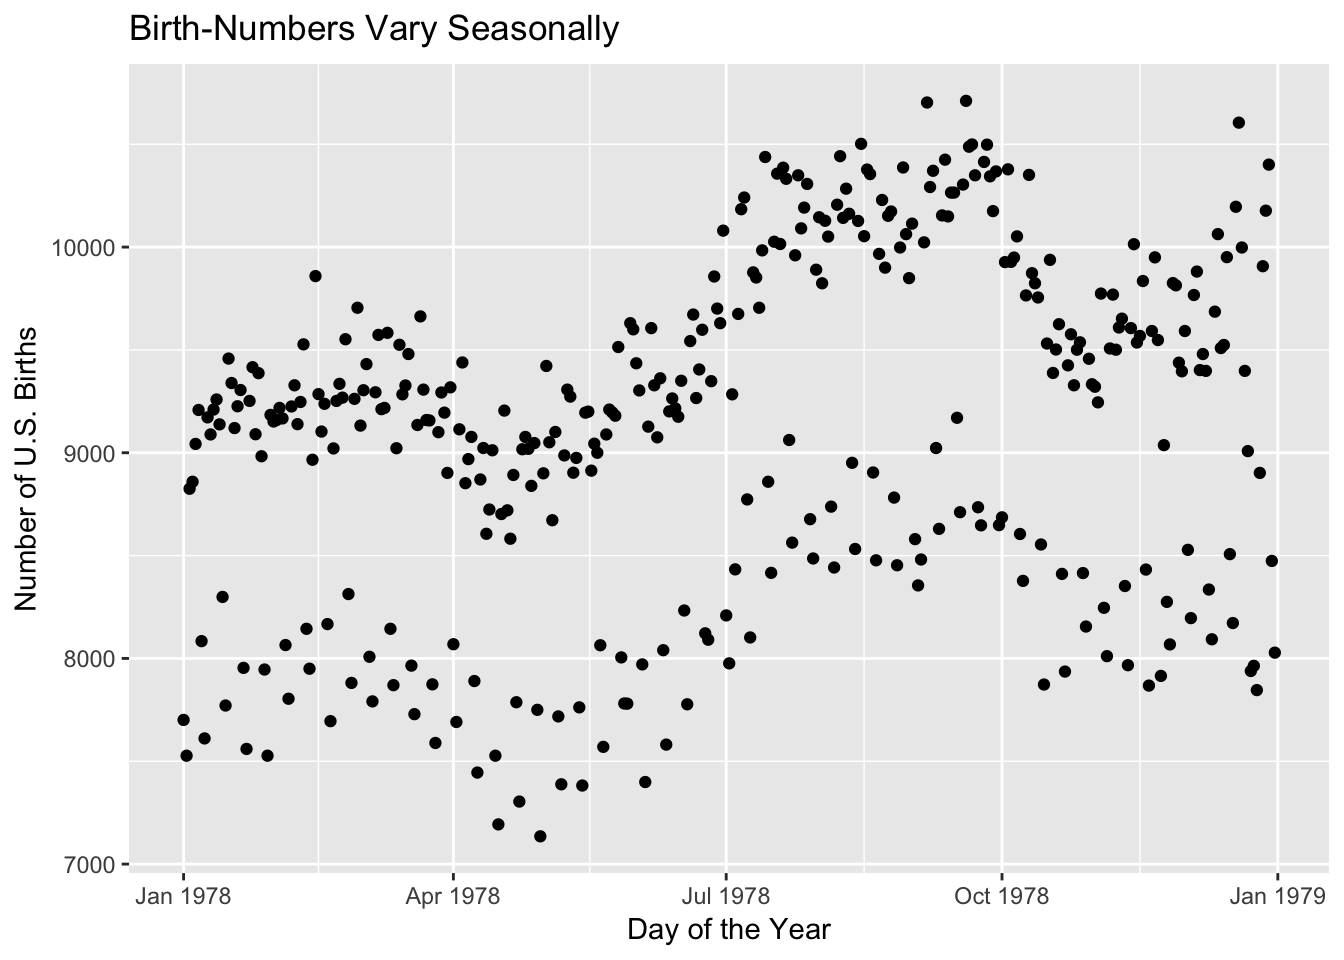
\includegraphics[width=0.6\linewidth]{r-notes_files/figure-latex/birthsplot-1} 

}

\caption{A simple scatterplot with R's ggplot2 graphics system.}\label{fig:birthsplot}
\end{figure}

Clearly the number of births varies seasonally: more babies are born in
late summer and early fall, whereas spring births are not as frequent.
But there is something mysterious about the plot: Why do there are
appear to be two clearly separated groups of days, one with considerably
more births than the other? What is going on here? As we learn to
program in R, we will gradually acquire the skills needed to answer this
and many other intriguing questions.

\section{Debugging}\label{idea-debugging}

It's easy to make mistakes when you program---even when you are very
experienced! Incorrect computer code is said to have a \emph{bug}, and
the art of finding bugs and correcting them is called \emph{debugging}.
\index{debugging}

Consider the following code:

\begin{Shaded}
\begin{Highlighting}[]
\NormalTok{scarecrowQuote <-}\StringTok{ "It is such an uncomfortable feeling to know one is a fool."}
\KeywordTok{paste}\NormalTok{(}\StringTok{"The Scarecrow says: "}\NormalTok{, scarecrowquote)}
\end{Highlighting}
\end{Shaded}

When we run it we get the following error message in the console:

\begin{verbatim}
## Error in paste("The Scarecrow says: ", scarecrowquote) : 
##  object 'scarecrowquote' not found
\end{verbatim}

R's error messages are often quite mysterious---they are intended to be
maximally useful to experienced R programmers---but it's always a good
idea to read them anyway. In this case the message clearly tells us the
problem: R cannot find the object \texttt{scarecrowquote} on its search
path. This prompt us to look more closely at the name
\texttt{scarecrow}, and sooner or later we will realize that we have a
misspelling: the variable that was actually defined was
\texttt{scarecrowQuote}, with a capital Q.

The correct code is:

\begin{Shaded}
\begin{Highlighting}[]
\NormalTok{scarecrowQuote <-}\StringTok{ "It is such an uncomfortable feeling to know one is a fool."}
\KeywordTok{paste}\NormalTok{(}\StringTok{"The Scarecrow says: "}\NormalTok{, scarecrowQuote)}
\end{Highlighting}
\end{Shaded}

\begin{verbatim}
## [1] "The Scarecrow says:  It is such an uncomfortable feeling to know one is a fool."
\end{verbatim}

\BeginKnitrBlock{rmdimportant}
Always bear in mind that R is case-sensitive!
\EndKnitrBlock{rmdimportant}

Here's another buggy bit of code:

\begin{Shaded}
\begin{Highlighting}[]
\NormalTok{SermonMountComment <-}\StringTok{ }\KeywordTok{paste}\NormalTok{(}\StringTok{"Oh, it's "}\NormalTok{blessed are the meek.}\StringTok{""}\NormalTok{,}
                     \StringTok{"}\CharTok{\textbackslash{}n}\StringTok{I'm glad they are getting something:}\CharTok{\textbackslash{}n}\StringTok{"}\NormalTok{,}
                     \StringTok{"they have a hell of a time."}\NormalTok{)}
\KeywordTok{cat}\NormalTok{(SermonMountComment)}
\end{Highlighting}
\end{Shaded}

The idea is to produce:

\begin{verbatim}
## Oh, it's "blessed are the meek.
## I'm glad they are getting something:
##  they have a hell of a time.
\end{verbatim}

But when we run the code we get the following result instead:

\begin{verbatim}
> rm(SermonMountComment)
> SermonMountComment <- paste("Oh, it's "blessed are the meek."",
Error: unexpected symbol in "SermonMountComment <- paste("Oh, it's "blessed"
>                             "\nI'm glad they are getting something: ",
Error: unexpected ',' in "                            "\nI'm glad they are getting something: ","
>                             "they have a hell of a time.")
Error: unexpected ')' in "                            "they have a hell of a time.")"
> cat(SermonMountComment)
Error in cat(SermonMountComment) : object 'SermonMountComment' not found
\end{verbatim}

This can be a bit more difficult to read. The problems appear to start
near the beginning of the construction of the string
\texttt{SermonMountComment}.

After looking at it a while we focus on the first string argument to the
\texttt{paste()} function:

\begin{quote}
\texttt{"Oh,\ it\textquotesingle{}s\ "blessed\ are\ the\ meek.""}
\end{quote}

We see that this string has quotes within quotes. Now R uses quotes as
\emph{delimiters} \index{delimiter} for strings: that is, quote-marks
indicate where a string begins and where it ends. Hence from R's point
of view, the first string consists of just:
\texttt{"Oh,\ it\textquotesingle{}s\ "}. But then there is no comma to
separate this string from the next string argument that the
\texttt{paste()} functions expects. Instead R sees the \texttt{b} in
\texttt{blessed}; that's an \emph{unexpected symbol}. Things go downhill
from there.

There are a couple of ways to correct the problem. One approach is to
use single quotes inside any string that is delimited with double
quotes, thus:

\begin{Shaded}
\begin{Highlighting}[]
\NormalTok{SermonMountComment <-}\StringTok{ }\KeywordTok{paste}\NormalTok{(}\StringTok{"Oh, it's 'blessed are the meek.'"}\NormalTok{,}
                     \StringTok{"}\CharTok{\textbackslash{}n}\StringTok{I'm glad they are getting something:}\CharTok{\textbackslash{}n}\StringTok{"}\NormalTok{,}
                     \StringTok{"they have a hell of a time."}\NormalTok{)}
\KeywordTok{cat}\NormalTok{(SermonMountComment)}
\end{Highlighting}
\end{Shaded}

\begin{verbatim}
## Oh, it's 'blessed are the meek.' 
## I'm glad they are getting something:
##  they have a hell of a time.
\end{verbatim}

On the other hand if you really want those double-quotes inside the
string, you can \emph{escape} their special meaning as string-delimiter
by prepending a backslash (\texttt{\textbackslash{}}) to them, thus:

\begin{Shaded}
\begin{Highlighting}[]
\NormalTok{SermonMountComment <-}\StringTok{ }\KeywordTok{paste}\NormalTok{(}\StringTok{"Oh, it's }\CharTok{\textbackslash{}"}\StringTok{blessed are the meek.}\CharTok{\textbackslash{}"}\StringTok{"}\NormalTok{,}
                     \StringTok{"}\CharTok{\textbackslash{}n}\StringTok{I'm glad they are getting something:}\CharTok{\textbackslash{}n}\StringTok{"}\NormalTok{,}
                     \StringTok{"they have a hell of a time."}\NormalTok{)}
\KeywordTok{cat}\NormalTok{(SermonMountComment)}
\end{Highlighting}
\end{Shaded}

\begin{verbatim}
## Oh, it's "blessed are the meek." 
## I'm glad they are getting something:
##  they have a hell of a time.
\end{verbatim}

There are a number of special characters that are formed by ``escaping''
the usual meaning of some other character. Some common examples are:

\begin{itemize}
\tightlist
\item
  \texttt{\textbackslash{}n}: produces a newline instead of \texttt{n}
\item
  \texttt{\textbackslash{}t}: produces a tab-space instead of \texttt{t}
\item
  \texttt{\textbackslash{}"}: produces an actual quote-mark, instead of
  beginning or ending a string.
\end{itemize}

Strings are a tricky topic in any computer programming language: in fact
we will devote all of Chapter \ref{strings} to them.

\newpage

\section*{Glossary}\label{idea-glossary}
\addcontentsline{toc}{section}{Glossary}

\begin{description}
\item[Computer Program \index{computer program}]
A sequence of instructions that performs a specific task when executed
by a computer.
\item[String]
A value in a computer program that constitutes text (as opposed to
numbers of some other type of data).
\item[Interactive Mode \index{interactive mode}]
A type of engagment between a human and a computer in which the computer
prompts the humand for data and/or commands and may respond with output
that the human can read and/or interpret.
\item[Read-Evaluate-Print Loop \index{REPL}]
An interactive cycle in which the R-interpreter reads an expression from
the console, evaluates it, and prints out the value to the console.
\item[Data Structure \index{data structure}]
A particular way of organizing information in an computer program so
that it can be used efficiently.
\item[Delimiter]
A character in a programing languages that is used to mark the beginning
and/or end of a value.
\end{description}

\newpage

\section*{Exercises}\label{idea-exercises}
\addcontentsline{toc}{section}{Exercises}

\begin{center}
\includegraphics[width=0.5\linewidth]{images/thinking} \end{center}

\begin{enumerate}
\def\labelenumi{\arabic{enumi}.}
\item
  Write a program that modifies the function \texttt{intro()} (see
  Section \ref{idea-functions}) so that the person who introduces him or
  herself states a favorite sport. For example, the result of the
  following function call:

\begin{Shaded}
\begin{Highlighting}[]
\KeywordTok{intro}\NormalTok{(}\DataTypeTok{name =} \StringTok{"Bettina"}\NormalTok{, }\DataTypeTok{type =} \StringTok{"human"}\NormalTok{, }\DataTypeTok{sport =} \StringTok{"lacrosse"}\NormalTok{)}
\end{Highlighting}
\end{Shaded}

  should be:

\begin{verbatim}
## Hello, I am a human.  
## My name is Bettina.
## My favorite sport is lacrosse.
\end{verbatim}
\item
  Write a program to produce the following output to the console:

\begin{verbatim}
## *
## **
## ***
## **
## *
\end{verbatim}
\item
  Suppose we want to \texttt{cat} ``Hello, World'' to the console, and
  we enter:

\begin{Shaded}
\begin{Highlighting}[]
\KeywordTok{cat}\NormalTok{(Hello, World!)}
\end{Highlighting}
\end{Shaded}

  What does R say? What did we do wrong?
\end{enumerate}

\chapter{Vectors}\label{vectors}

\begin{figure}[!h]

{\centering 
\includegraphics[width=0.24\linewidth]{images/yarn} 
\includegraphics[width=0.24\linewidth]{images/yarn} 
\includegraphics[width=0.24\linewidth]{images/yarn} 
\includegraphics[width=0.24\linewidth]{images/yarn} 

}

\caption{`rep(yarn, times = 4)`.}\label{fig:vector-of-strings}
\end{figure}

This Chapter gets you started officially with R. While the theme is
\emph{vectors}\index{vector}, the most important data structure in R,
we'll learn also about variables and variable names, vector types,
reserved words, assignment and many of R's basic operators.

\newpage

\section{What is a Vector?}\label{what-is-a-vector}

If you have heard of vectors before in mathematics, you might think of a
vector as something that has a magnitude and a direction, and that can
be represented by a sequence of numbers. In its notion of a vector, R
keeps the idea of a sequence but discards magnitude and direction. The
notion of ``numbers'' isn't even necessary.

For R, a vector is simply a sequence of elements. There are two general
sort of vectors:

\begin{itemize}
\tightlist
\item
  \emph{atomic} vectors that come in one of six forms called
  \emph{vector types};\index{vector type}
\item
  non-atomic vectors, called \emph{lists}, whose elements can be any
  sort of R-object at all.
\end{itemize}

For now we'll just study atomic vectors. Let's make a few vectors, as
examples.

We can make a vector of numbers using the
\texttt{c()}\index{R-functions!c()@\texttt{c()}} function:

\begin{Shaded}
\begin{Highlighting}[]
\NormalTok{numVec <-}\StringTok{ }\KeywordTok{c}\NormalTok{(}\FloatTok{23.2}\NormalTok{, }\DecValTok{45}\NormalTok{, }\DecValTok{631}\NormalTok{, -}\DecValTok{273}\NormalTok{, }\DecValTok{0}\NormalTok{, }\FloatTok{48.371}\NormalTok{, }\DecValTok{100000}\NormalTok{,}
            \DecValTok{85}\NormalTok{, }\DecValTok{92}\NormalTok{, -}\DecValTok{236}\NormalTok{, }\DecValTok{8546}\NormalTok{, }\DecValTok{98774}\NormalTok{, }\DecValTok{0}\NormalTok{, }\DecValTok{0}\NormalTok{, }\DecValTok{1}\NormalTok{, }\DecValTok{3}\NormalTok{)}
\NormalTok{numVec}
\end{Highlighting}
\end{Shaded}

\begin{verbatim}
##  [1]     23.200     45.000    631.000   -273.000      0.000     48.371
##  [7] 100000.000     85.000     92.000   -236.000   8546.000  98774.000
## [13]      0.000      0.000      1.000      3.000
\end{verbatim}

You can think of \texttt{c} as standing for ``combine.'' \texttt{c()}
takes its arguments, all of which are separated by commas, and combines
them to make a vector.

If you closely examine the above output, you'll notice that R printed
out all of the numerical values in the vector to three decimal places,
which happened to be the largest number of decimal places we assigned to
any of the numbers that made up \texttt{numVec}. You'll also notice the
numbers in brackets at the beginning of the lines. Each number
represents the position within the vector occupied by the first element
of the vector that is printed on the line. The position of an element in
a vector is called its \emph{index}\index{index}. Reporting the indices
of leading elements helps you locate particular elements in the output.

\subsection{Types of Atomic Vectors}\label{types-of-atomic-vectors}

The numbers in \texttt{numVec} are what programmers call
\emph{double-precision} numbers. You can verify this for yourself with
the \texttt{typeof()}\index{R-functions!typeof()@\texttt{typeof()}}
function:

\begin{Shaded}
\begin{Highlighting}[]
\KeywordTok{typeof}\NormalTok{(numVec)}
\end{Highlighting}
\end{Shaded}

\begin{verbatim}
## [1] "double"
\end{verbatim}

The \texttt{typeof()} function returns the type of any object in R. As
far as vectors are concerned, there are six possible types, of which we
will deal with only four:

\begin{itemize}
\tightlist
\item
  \texttt{double}\index{double}
\item
  \texttt{integer}
\item
  \texttt{character}
\item
  \texttt{logical}
\end{itemize}

Let's look at examples of the other types. Here is a vector of type
\texttt{integer}\index{integer}:

\begin{Shaded}
\begin{Highlighting}[]
\NormalTok{intVec <-}\StringTok{ }\KeywordTok{c}\NormalTok{(3L, 17L, -22L, 45L)}
\NormalTok{intVec}
\end{Highlighting}
\end{Shaded}

\begin{verbatim}
## [1]   3  17 -22  45
\end{verbatim}

The \texttt{L} after each number signifies to R that the number should
be stored in memory as an integer, rather than in double-precision
format. Officially, the type is \texttt{integer}:

\begin{Shaded}
\begin{Highlighting}[]
\KeywordTok{typeof}\NormalTok{(intVec)}
\end{Highlighting}
\end{Shaded}

\begin{verbatim}
## [1] "integer"
\end{verbatim}

You should know that if you left off one or more of the \texttt{L}'s,
then R would create a vector of type \texttt{double}:

\begin{Shaded}
\begin{Highlighting}[]
\NormalTok{numVec2 <-}\StringTok{ }\KeywordTok{c}\NormalTok{(}\DecValTok{3}\NormalTok{, }\DecValTok{17}\NormalTok{, -}\DecValTok{22}\NormalTok{, }\DecValTok{45}\NormalTok{)}
\KeywordTok{typeof}\NormalTok{(numVec2)}
\end{Highlighting}
\end{Shaded}

\begin{verbatim}
## [1] "double"
\end{verbatim}

We won't work much with integer-type vectors, but you'll see them out in
the wild.

We can also make vectors out of pieces of text called
\emph{strings}\index{string}: these are called
\emph{character}\index{character} vectors. As noted in the previous
chapter, we use quotes to delimit strings:

\begin{Shaded}
\begin{Highlighting}[]
\NormalTok{strVec <-}\StringTok{ }\KeywordTok{c}\NormalTok{(}\StringTok{"Brains"}\NormalTok{, }\StringTok{"are"}\NormalTok{, }\StringTok{"not"}\NormalTok{, }\StringTok{"the"}\NormalTok{, }\StringTok{"best"}\NormalTok{, }
            \StringTok{"things"}\NormalTok{, }\StringTok{"in"}\NormalTok{, }\StringTok{"the"}\NormalTok{, }\StringTok{"world"}\NormalTok{, }\StringTok{"93.2"}\NormalTok{)}
\NormalTok{strVec}
\end{Highlighting}
\end{Shaded}

\begin{verbatim}
##  [1] "Brains" "are"    "not"    "the"    "best"   "things" "in"    
##  [8] "the"    "world"  "93.2"
\end{verbatim}

\begin{Shaded}
\begin{Highlighting}[]
\KeywordTok{typeof}\NormalTok{(strVec)}
\end{Highlighting}
\end{Shaded}

\begin{verbatim}
## [1] "character"
\end{verbatim}

Notice that \texttt{"93.2"} makes a string, not a number.

The last type of vectors to consider are the
\texttt{logical}\index{logical} vectors. Here is an example:

\begin{Shaded}
\begin{Highlighting}[]
\NormalTok{logVec <-}\StringTok{ }\KeywordTok{c}\NormalTok{(}\OtherTok{TRUE}\NormalTok{, }\OtherTok{FALSE}\NormalTok{, T, T, F, F, }\OtherTok{FALSE}\NormalTok{)}
\NormalTok{logVec}
\end{Highlighting}
\end{Shaded}

\begin{verbatim}
## [1]  TRUE FALSE  TRUE  TRUE FALSE FALSE FALSE
\end{verbatim}

In order to represent a logical value you can use:

\begin{itemize}
\tightlist
\item
  \texttt{TRUE} or \texttt{T} to represent truth;
\item
  \texttt{FALSE} or \texttt{F} to represent falsity.
\end{itemize}

You can't represent truth or falsity any other way. If you try anything
else---like the following---you get an error:

\begin{Shaded}
\begin{Highlighting}[]
\NormalTok{badVec <-}\StringTok{ }\KeywordTok{c}\NormalTok{(}\OtherTok{TRUE}\NormalTok{, false)}
\end{Highlighting}
\end{Shaded}

\begin{verbatim}
## Error: object 'false' not found
\end{verbatim}

\subsection{Coercion}\label{coercion}

What would happen if you tried to represent falsity with the string
\texttt{"false"}?

\begin{Shaded}
\begin{Highlighting}[]
\NormalTok{newVector <-}\StringTok{ }\KeywordTok{c}\NormalTok{(}\OtherTok{TRUE}\NormalTok{, }\StringTok{"false"}\NormalTok{)}
\NormalTok{newVector}
\end{Highlighting}
\end{Shaded}

\begin{verbatim}
## [1] "TRUE"  "false"
\end{verbatim}

\texttt{newVector} is not a logical vector. Check it out:

\begin{Shaded}
\begin{Highlighting}[]
\KeywordTok{typeof}\NormalTok{(newVector)}
\end{Highlighting}
\end{Shaded}

\begin{verbatim}
## [1] "character"
\end{verbatim}

In order to understand what just happened here, you must recall that all
of the elements of an atomic vector have to be of the same type. If the
\texttt{c()} function is presented with values of different types, then
R follows a set of internal rules to \emph{coerce}\index{coercion} some
of the values to a new type in such a way that all resulting values are
of the same type. You don't need to know all of the coercion rules, but
it's worth noting that

\begin{itemize}
\tightlist
\item
  \texttt{character} beats \texttt{double},
\item
  which in turn beats \texttt{integer},
\item
  which in in turn beats \texttt{logical}.
\end{itemize}

The following examples show this:

\begin{Shaded}
\begin{Highlighting}[]
\KeywordTok{typeof}\NormalTok{(}\KeywordTok{c}\NormalTok{(}\StringTok{"one"}\NormalTok{, }\DecValTok{1}\NormalTok{, 1L, }\OtherTok{TRUE}\NormalTok{))}
\end{Highlighting}
\end{Shaded}

\begin{verbatim}
## [1] "character"
\end{verbatim}

\begin{Shaded}
\begin{Highlighting}[]
\KeywordTok{typeof}\NormalTok{(}\KeywordTok{c}\NormalTok{(}\DecValTok{1}\NormalTok{, 1L, }\OtherTok{TRUE}\NormalTok{))}
\end{Highlighting}
\end{Shaded}

\begin{verbatim}
## [1] "double"
\end{verbatim}

\begin{Shaded}
\begin{Highlighting}[]
\KeywordTok{typeof}\NormalTok{(}\KeywordTok{c}\NormalTok{(1L, }\OtherTok{TRUE}\NormalTok{))}
\end{Highlighting}
\end{Shaded}

\begin{verbatim}
## [1] "integer"
\end{verbatim}

Automatic coercion can be convenient in some circumstances, but in
others it can give unexpected results. It's best to keep track of what
types you are dealing with and to exercise caution when combining values
to make new vectors.

You can also coerce vectors ``manually'' with the functions:

\begin{itemize}
\tightlist
\item
  \texttt{as.numeric()}
  \index{R-functions!as.numeric()@\texttt{as.numeric()}};
\item
  \texttt{as.integer()}
  \index{R-functions!as.integer()@\texttt{as.integer()}};
\item
  \texttt{as.character()}
  \index{R-functions!as.character()@\texttt{as.character()}};
\item
  \texttt{as.logical()}
  \index{R-functions!as.logical()@\texttt{as.logical()}}.
\end{itemize}

Here are some examples:

\begin{Shaded}
\begin{Highlighting}[]
\NormalTok{numVec <-}\StringTok{ }\KeywordTok{c}\NormalTok{(}\DecValTok{3}\NormalTok{, }\FloatTok{2.5}\NormalTok{, -}\FloatTok{7.32}\NormalTok{, }\DecValTok{0}\NormalTok{)}
\KeywordTok{as.character}\NormalTok{(numVec)}
\end{Highlighting}
\end{Shaded}

\begin{verbatim}
## [1] "3"     "2.5"   "-7.32" "0"
\end{verbatim}

\begin{Shaded}
\begin{Highlighting}[]
\KeywordTok{as.integer}\NormalTok{(numVec)}
\end{Highlighting}
\end{Shaded}

\begin{verbatim}
## [1]  3  2 -7  0
\end{verbatim}

\begin{Shaded}
\begin{Highlighting}[]
\KeywordTok{as.logical}\NormalTok{(numVec)}
\end{Highlighting}
\end{Shaded}

\begin{verbatim}
## [1]  TRUE  TRUE  TRUE FALSE
\end{verbatim}

Note that in coercion from numerical to logical, the number 0 becomes
\texttt{FALSE} and all non-zero numbers become \texttt{TRUE}.

\subsection{Combining Vectors}\label{combining-vectors}

You can combine vectors you have already created to make new, bigger
ones:

\begin{Shaded}
\begin{Highlighting}[]
\NormalTok{numVec1 <-}\StringTok{ }\KeywordTok{c}\NormalTok{(}\DecValTok{5}\NormalTok{, }\DecValTok{3}\NormalTok{, }\DecValTok{10}\NormalTok{)}
\NormalTok{numVec2 <-}\StringTok{ }\KeywordTok{c}\NormalTok{(}\DecValTok{1}\NormalTok{, }\DecValTok{2}\NormalTok{, }\DecValTok{3}\NormalTok{, }\DecValTok{4}\NormalTok{, }\DecValTok{5}\NormalTok{, }\DecValTok{6}\NormalTok{)}
\NormalTok{numCombined <-}\StringTok{ }\KeywordTok{c}\NormalTok{(numVec1, numVec2)}
\NormalTok{numCombined}
\end{Highlighting}
\end{Shaded}

\begin{verbatim}
## [1]  5  3 10  1  2  3  4  5  6
\end{verbatim}

You can see here that vectors are different from sets: they are allowed
to repeat the same value in different indices, as we see in the case of
the 3's above.

\subsection{\texorpdfstring{NA Values
\index{NA}}{NA Values }}\label{na-values}

Consider the following vector, which we may think of as recording the
heights of people, in inches:

\begin{Shaded}
\begin{Highlighting}[]
\NormalTok{heights <-}\StringTok{ }\KeywordTok{c}\NormalTok{(}\DecValTok{72}\NormalTok{, }\DecValTok{70}\NormalTok{, }\DecValTok{69}\NormalTok{, }\DecValTok{58}\NormalTok{, }\OtherTok{NA}\NormalTok{, }\DecValTok{45}\NormalTok{)}
\end{Highlighting}
\end{Shaded}

The \texttt{NA} in the fifth position of the vector is a special value
that may be considered to mean ``Not Assigned.''" It's R's way of
letting us indicate that a value was not recorded or has gone missing
for some reason.

\subsection{\texorpdfstring{``Everything in R is a
Vector''}{Everything in R is a Vector}}\label{everything-in-r-is-a-vector}

Some folks say that everything in R is a vector. That's a bit of an
exaggeration but it's remarkably close to the truth.

And yet it seems implausible. What about the elements of an atomic
vector, for instance? A single element doesn't look at all like a
vector: it's a value, not a \emph{sequence} of values.

Or so we might think. But really, in R there are no ``single values''
that can exist by themselves. Consider, for instance, what we think of
as the number 17:

\begin{Shaded}
\begin{Highlighting}[]
\DecValTok{17}
\end{Highlighting}
\end{Shaded}

\begin{verbatim}
## [1] 17
\end{verbatim}

See the \texttt{{[}1{]}} in front, in the output above? It indicates
that the line begins with the \emph{first element} of a vector. So 17
doesn't exist on its own: it exists a vector of type \texttt{double}---a
vector of length 1.

Even \texttt{NA} is, all along, a vector of length 1

\begin{Shaded}
\begin{Highlighting}[]
\OtherTok{NA}
\end{Highlighting}
\end{Shaded}

\begin{verbatim}
## [1] NA
\end{verbatim}

It is of type \texttt{logical}:

\begin{Shaded}
\begin{Highlighting}[]
\KeywordTok{typeof}\NormalTok{(}\OtherTok{NA}\NormalTok{)}
\end{Highlighting}
\end{Shaded}

\begin{verbatim}
## [1] "logical"
\end{verbatim}

Note that even the type of \texttt{NA} evaluates, in R, to a vector: a
character vector of length 1 whose only element is the string
``logical''!

\subsection{Named Vectors}\label{named-vectors}

The elements of a vector can have names, if we like:

\begin{Shaded}
\begin{Highlighting}[]
\NormalTok{ages <-}\StringTok{ }\KeywordTok{c}\NormalTok{(}\DataTypeTok{Bettina =} \DecValTok{32}\NormalTok{, }\DataTypeTok{Chris =} \DecValTok{64}\NormalTok{, }\DataTypeTok{Ramesh =} \DecValTok{101}\NormalTok{)}
\NormalTok{ages}
\end{Highlighting}
\end{Shaded}

\begin{verbatim}
## Bettina   Chris  Ramesh 
##      32      64     101
\end{verbatim}

Having names doesn't keep the vector from being a vector of type
\texttt{double}: it has to be \texttt{double} because its elements are
\texttt{double}.

\begin{Shaded}
\begin{Highlighting}[]
\KeywordTok{typeof}\NormalTok{(ages)}
\end{Highlighting}
\end{Shaded}

\begin{verbatim}
## [1] "double"
\end{verbatim}

We can names the elements of a vector when we create it with
\texttt{c()}, or we can name them later on. One way to do this is with
the \texttt{names()}\index{R-functions!names()@\texttt{names()}}
function:

\begin{Shaded}
\begin{Highlighting}[]
\KeywordTok{names}\NormalTok{(heights) <-}\StringTok{ }\KeywordTok{c}\NormalTok{(}\StringTok{"Scarecrow"}\NormalTok{, }\StringTok{"Tinman"}\NormalTok{, }\StringTok{"Lion"}\NormalTok{, }\StringTok{"Dorothy"}\NormalTok{, }\StringTok{"Toto"}\NormalTok{, }\StringTok{"Boq"}\NormalTok{)}
\NormalTok{heights}
\end{Highlighting}
\end{Shaded}

\begin{verbatim}
## Scarecrow    Tinman      Lion   Dorothy      Toto       Boq 
##        72        70        69        58        NA        45
\end{verbatim}

\subsection{Special Character Vectors}\label{special-character-vectors}

R comes with two handy, predefined character vectors:

\begin{Shaded}
\begin{Highlighting}[]
\NormalTok{letters}
\end{Highlighting}
\end{Shaded}

\begin{verbatim}
##  [1] "a" "b" "c" "d" "e" "f" "g" "h" "i" "j" "k" "l" "m" "n" "o" "p" "q"
## [18] "r" "s" "t" "u" "v" "w" "x" "y" "z"
\end{verbatim}

\begin{Shaded}
\begin{Highlighting}[]
\NormalTok{LETTERS}
\end{Highlighting}
\end{Shaded}

\begin{verbatim}
##  [1] "A" "B" "C" "D" "E" "F" "G" "H" "I" "J" "K" "L" "M" "N" "O" "P" "Q"
## [18] "R" "S" "T" "U" "V" "W" "X" "Y" "Z"
\end{verbatim}

We will make use of them from time to
time.\index{R-constants!letters@\texttt{letters}}\index{R-constants!LETTER@\texttt{LETTERS}}

\subsection{Length of Vectors}\label{length-of-vectors}

The \texttt{length()}
function\index{R-functions!length()@\texttt{length()}} tells us how many
elements a vector has:

\begin{Shaded}
\begin{Highlighting}[]
\KeywordTok{length}\NormalTok{(heights)}
\end{Highlighting}
\end{Shaded}

\begin{verbatim}
## [1] 6
\end{verbatim}

\section{Constructing Patterned
Vectors}\label{constructing-patterned-vectors}

Quite often we need to make lengthy vectors that follow simple patterns.
R has a few functions to assist us in these tasks.

\subsection{Sequencing}\label{sequencing}

Consider the \texttt{seq()}\index{R-functions!seq()@\texttt{seq()}}
function:

\begin{Shaded}
\begin{Highlighting}[]
\KeywordTok{seq}\NormalTok{(}\DataTypeTok{from =} \DecValTok{5}\NormalTok{, }\DataTypeTok{to =} \DecValTok{15}\NormalTok{, }\DataTypeTok{by =} \DecValTok{1}\NormalTok{)}
\end{Highlighting}
\end{Shaded}

\begin{verbatim}
##  [1]  5  6  7  8  9 10 11 12 13 14 15
\end{verbatim}

The default value of the parameter \texttt{by} is 1, so we could get the
same thing with:

\begin{Shaded}
\begin{Highlighting}[]
\KeywordTok{seq}\NormalTok{(}\DataTypeTok{from =} \DecValTok{5}\NormalTok{, }\DataTypeTok{to =} \DecValTok{15}\NormalTok{)}
\end{Highlighting}
\end{Shaded}

\begin{verbatim}
##  [1]  5  6  7  8  9 10 11 12 13 14 15
\end{verbatim}

Further reduction in typing may be achieved as long as we remember the
order in which R expects the parameters (\texttt{from} before
\texttt{to}, then \texttt{by} if supplied):

\begin{Shaded}
\begin{Highlighting}[]
\KeywordTok{seq}\NormalTok{(}\DecValTok{5}\NormalTok{, }\DecValTok{15}\NormalTok{)}
\end{Highlighting}
\end{Shaded}

\begin{verbatim}
##  [1]  5  6  7  8  9 10 11 12 13 14 15
\end{verbatim}

Some more complex examples:

\begin{Shaded}
\begin{Highlighting}[]
\KeywordTok{seq}\NormalTok{(}\DecValTok{3}\NormalTok{, }\DecValTok{15}\NormalTok{, }\DecValTok{2}\NormalTok{)}
\end{Highlighting}
\end{Shaded}

\begin{verbatim}
## [1]  3  5  7  9 11 13 15
\end{verbatim}

\begin{Shaded}
\begin{Highlighting}[]
\KeywordTok{seq}\NormalTok{(}\DecValTok{0}\NormalTok{, }\DecValTok{1}\NormalTok{, }\FloatTok{0.1}\NormalTok{)}
\end{Highlighting}
\end{Shaded}

\begin{verbatim}
##  [1] 0.0 0.1 0.2 0.3 0.4 0.5 0.6 0.7 0.8 0.9 1.0
\end{verbatim}

R will go up to the \texttt{to} value, but not past it:

\begin{Shaded}
\begin{Highlighting}[]
\KeywordTok{seq}\NormalTok{(}\DecValTok{3}\NormalTok{, }\DecValTok{16}\NormalTok{, }\DecValTok{2}\NormalTok{)}
\end{Highlighting}
\end{Shaded}

\begin{verbatim}
## [1]  3  5  7  9 11 13 15
\end{verbatim}

Negative steps are fine:

\begin{Shaded}
\begin{Highlighting}[]
\KeywordTok{seq}\NormalTok{(}\DecValTok{5}\NormalTok{, -}\DecValTok{4}\NormalTok{, -}\DecValTok{1}\NormalTok{)}
\end{Highlighting}
\end{Shaded}

\begin{verbatim}
##  [1]  5  4  3  2  1  0 -1 -2 -3 -4
\end{verbatim}

The \emph{colon operator} \texttt{:} is a convenient abbreviation for
\texttt{seq}:\index{R-operators!: (sequencing)}

\begin{Shaded}
\begin{Highlighting}[]
\DecValTok{1}\NormalTok{:}\DecValTok{5} \CommentTok{# 1 is from, 5 is to}
\end{Highlighting}
\end{Shaded}

\begin{verbatim}
## [1] 1 2 3 4 5
\end{verbatim}

If the \texttt{from} number is greater than the \texttt{to} number the
step for the colon operator is -1:

\begin{Shaded}
\begin{Highlighting}[]
\DecValTok{5}\NormalTok{:}\DecValTok{1}
\end{Highlighting}
\end{Shaded}

\begin{verbatim}
## [1] 5 4 3 2 1
\end{verbatim}

\subsection{Repeating}\label{repeating}

With \texttt{rep()}\index{R-functions!rep()@\texttt{rep()}} we may
repeat a given vector as many times as we like:

\begin{Shaded}
\begin{Highlighting}[]
\KeywordTok{rep}\NormalTok{(}\DecValTok{3}\NormalTok{, }\DataTypeTok{times =} \DecValTok{5}\NormalTok{)}
\end{Highlighting}
\end{Shaded}

\begin{verbatim}
## [1] 3 3 3 3 3
\end{verbatim}

We can apply \texttt{rep()} to a vector of length greater than 1:

\begin{Shaded}
\begin{Highlighting}[]
\NormalTok{vec <-}\StringTok{ }\KeywordTok{c}\NormalTok{(}\DecValTok{7}\NormalTok{, }\DecValTok{3}\NormalTok{, }\DecValTok{4}\NormalTok{)}
\KeywordTok{rep}\NormalTok{(vec, }\DataTypeTok{times =} \DecValTok{3}\NormalTok{)}
\end{Highlighting}
\end{Shaded}

\begin{verbatim}
## [1] 7 3 4 7 3 4 7 3 4
\end{verbatim}

\texttt{rep()} applies perfectly well to character-vectors:

\begin{Shaded}
\begin{Highlighting}[]
\KeywordTok{rep}\NormalTok{(}\StringTok{"Toto"}\NormalTok{, }\DecValTok{4}\NormalTok{)}
\end{Highlighting}
\end{Shaded}

\begin{verbatim}
## [1] "Toto" "Toto" "Toto" "Toto"
\end{verbatim}

\texttt{rep()} also takes an \texttt{each} parameter that determines how
many times each element of the given vector will be repeated before the
\texttt{times} parameter is applied. This is best illustrated with an
example:

\begin{Shaded}
\begin{Highlighting}[]
\NormalTok{vec <-}\StringTok{ }\KeywordTok{c}\NormalTok{(}\DecValTok{7}\NormalTok{, }\DecValTok{3}\NormalTok{, }\DecValTok{4}\NormalTok{)}
\KeywordTok{rep}\NormalTok{(vec, }\DataTypeTok{each =} \DecValTok{2}\NormalTok{, }\DataTypeTok{times =} \DecValTok{3}\NormalTok{)}
\end{Highlighting}
\end{Shaded}

\begin{verbatim}
##  [1] 7 7 3 3 4 4 7 7 3 3 4 4 7 7 3 3 4 4
\end{verbatim}

If we combine \texttt{seq()} and \texttt{rep()} we can create fairly
complex patterns concisely:

\begin{Shaded}
\begin{Highlighting}[]
\NormalTok{vec <-}\StringTok{ }\KeywordTok{seq}\NormalTok{(}\DecValTok{5}\NormalTok{, -}\DecValTok{3}\NormalTok{, -}\DecValTok{2}\NormalTok{)}
\KeywordTok{rep}\NormalTok{(vec, }\DataTypeTok{each =} \DecValTok{2}\NormalTok{, }\DataTypeTok{times =} \DecValTok{2}\NormalTok{)}
\end{Highlighting}
\end{Shaded}

\begin{verbatim}
##  [1]  5  5  3  3  1  1 -1 -1 -3 -3  5  5  3  3  1  1 -1 -1 -3 -3
\end{verbatim}

In order to create fifty 10's followed by fifty 30's followed by fifty
50's I would write:

\begin{Shaded}
\begin{Highlighting}[]
\KeywordTok{rep}\NormalTok{(}\KeywordTok{seq}\NormalTok{(}\DecValTok{10}\NormalTok{, }\DecValTok{50}\NormalTok{, }\DecValTok{20}\NormalTok{), }\DataTypeTok{each =} \DecValTok{50}\NormalTok{)}
\end{Highlighting}
\end{Shaded}

\section{Subsetting Vectors}\label{subsetting-vectors}

Quite often we need to select one or more elements from a vector. The
\emph{subsetting operator} \texttt{{[}}
\index{R-operators![ (subsetting)} allows us to do this.

Recall the vector \texttt{heights}:

\begin{Shaded}
\begin{Highlighting}[]
\NormalTok{heights}
\end{Highlighting}
\end{Shaded}

\begin{verbatim}
## Scarecrow    Tinman      Lion   Dorothy      Toto       Boq 
##        72        70        69        58        NA        45
\end{verbatim}

If we want the fourth element, we ask for it with the subsetting
operator like this:

\begin{Shaded}
\begin{Highlighting}[]
\NormalTok{heights[}\DecValTok{4}\NormalTok{]}
\end{Highlighting}
\end{Shaded}

\begin{verbatim}
## Dorothy 
##      58
\end{verbatim}

If we want two or more elements, then we specify their indices in a
vector. Thus, to get the first and fifth elements, we might do this:

\begin{Shaded}
\begin{Highlighting}[]
\NormalTok{desired <-}\StringTok{ }\KeywordTok{c}\NormalTok{(}\DecValTok{1}\NormalTok{,}\DecValTok{5}\NormalTok{)}
\NormalTok{heights[desired]}
\end{Highlighting}
\end{Shaded}

\begin{verbatim}
## Scarecrow      Toto 
##        72        NA
\end{verbatim}

We could also ask for them directly:

\begin{Shaded}
\begin{Highlighting}[]
\NormalTok{heights[}\KeywordTok{c}\NormalTok{(}\DecValTok{1}\NormalTok{,}\DecValTok{5}\NormalTok{)]}
\end{Highlighting}
\end{Shaded}

\begin{verbatim}
## Scarecrow      Toto 
##        72        NA
\end{verbatim}

Negative numbers are significant in subsetting:

\begin{Shaded}
\begin{Highlighting}[]
\NormalTok{heights[-}\DecValTok{2}\NormalTok{] }\CommentTok{#select all but second element}
\end{Highlighting}
\end{Shaded}

\begin{verbatim}
## Scarecrow      Lion   Dorothy      Toto       Boq 
##        72        69        58        NA        45
\end{verbatim}

\begin{Shaded}
\begin{Highlighting}[]
\NormalTok{heights[-}\KeywordTok{c}\NormalTok{(}\DecValTok{1}\NormalTok{,}\DecValTok{3}\NormalTok{)]  }\CommentTok{# all but first and third}
\end{Highlighting}
\end{Shaded}

\begin{verbatim}
##  Tinman Dorothy    Toto     Boq 
##      70      58      NA      45
\end{verbatim}

If you specify a nonexistent index, you get \texttt{NA}, the reasonable
result:

\begin{Shaded}
\begin{Highlighting}[]
\NormalTok{heights[}\DecValTok{7}\NormalTok{]}
\end{Highlighting}
\end{Shaded}

\begin{verbatim}
## <NA> 
##   NA
\end{verbatim}

Patterned vectors are quite useful for subsetting. If you want the first
three elements of \texttt{heights}, you don't have to type
\texttt{heights{[}c(1,2,3){]}}. Instead you can just say:

\begin{Shaded}
\begin{Highlighting}[]
\NormalTok{heights[}\DecValTok{1}\NormalTok{:}\DecValTok{3}\NormalTok{]}
\end{Highlighting}
\end{Shaded}

\begin{verbatim}
## Scarecrow    Tinman      Lion 
##        72        70        69
\end{verbatim}

The following gives the same as \texttt{heights}:

\begin{Shaded}
\begin{Highlighting}[]
\NormalTok{heights[}\DecValTok{1}\NormalTok{:}\KeywordTok{length}\NormalTok{(heights)]}
\end{Highlighting}
\end{Shaded}

\begin{verbatim}
## Scarecrow    Tinman      Lion   Dorothy      Toto       Boq 
##        72        70        69        58        NA        45
\end{verbatim}

If you desire to quickly provide names for a vector, subsetting can
help:

\begin{Shaded}
\begin{Highlighting}[]
\NormalTok{vec <-}\StringTok{ }\KeywordTok{c}\NormalTok{(}\DecValTok{23}\NormalTok{, }\DecValTok{14}\NormalTok{, }\DecValTok{82}\NormalTok{, }\DecValTok{33}\NormalTok{, }\DecValTok{33}\NormalTok{, }\DecValTok{45}\NormalTok{)}
\KeywordTok{names}\NormalTok{(vec) <-}\StringTok{ }\NormalTok{LETTERS[}\DecValTok{1}\NormalTok{:}\KeywordTok{length}\NormalTok{(vec)]}
\NormalTok{vec}
\end{Highlighting}
\end{Shaded}

\begin{verbatim}
##  A  B  C  D  E  F 
## 23 14 82 33 33 45
\end{verbatim}

If a vector has names we can refer to its elements using the subsetting
operator and those names:

\begin{Shaded}
\begin{Highlighting}[]
\NormalTok{heights[}\StringTok{"Tinman"}\NormalTok{]}
\end{Highlighting}
\end{Shaded}

\begin{verbatim}
## Tinman 
##     70
\end{verbatim}

\begin{Shaded}
\begin{Highlighting}[]
\NormalTok{heights[}\KeywordTok{c}\NormalTok{(}\StringTok{"Scarecrow"}\NormalTok{, }\StringTok{"Boq"}\NormalTok{)]}
\end{Highlighting}
\end{Shaded}

\begin{verbatim}
## Scarecrow       Boq 
##        72        45
\end{verbatim}

Finally, we can use subsetting to modify parts of a vector. For example,
Dorothy's height is reported as:

\begin{Shaded}
\begin{Highlighting}[]
\NormalTok{heights[}\StringTok{"Dorothy"}\NormalTok{]}
\end{Highlighting}
\end{Shaded}

\begin{verbatim}
## Dorothy 
##      58
\end{verbatim}

If Dorothy grows two inches, then we can modify her height as follows:

\begin{Shaded}
\begin{Highlighting}[]
\NormalTok{heights[}\StringTok{"Dorothy"}\NormalTok{] <-}\StringTok{ }\DecValTok{60}
\end{Highlighting}
\end{Shaded}

We can replace more than one element, of course. Thus:

\begin{Shaded}
\begin{Highlighting}[]
\NormalTok{heights[}\KeywordTok{c}\NormalTok{(}\StringTok{"Scarecrow"}\NormalTok{, }\StringTok{"Boq"}\NormalTok{)] <-}\StringTok{ }\KeywordTok{c}\NormalTok{(}\DecValTok{73}\NormalTok{, }\DecValTok{46}\NormalTok{)}
\end{Highlighting}
\end{Shaded}

The subset of indices may be as complex as you like:

\begin{Shaded}
\begin{Highlighting}[]
\NormalTok{vec <-}\StringTok{ }\KeywordTok{c}\NormalTok{(}\DecValTok{3}\NormalTok{,}\DecValTok{4}\NormalTok{,}\DecValTok{5}\NormalTok{,}\DecValTok{6}\NormalTok{,}\DecValTok{7}\NormalTok{,}\DecValTok{8}\NormalTok{)}
\NormalTok{vec[}\KeywordTok{seq}\NormalTok{(}\DataTypeTok{from =} \DecValTok{2}\NormalTok{, }\DataTypeTok{to =} \DecValTok{6}\NormalTok{, }\DataTypeTok{by =} \DecValTok{2}\NormalTok{)] <-}\StringTok{ }\KeywordTok{c}\NormalTok{(}\DecValTok{100}\NormalTok{, }\DecValTok{200}\NormalTok{, }\DecValTok{300}\NormalTok{)}
\NormalTok{vec}
\end{Highlighting}
\end{Shaded}

\begin{verbatim}
## [1]   3 100   5 200   7 300
\end{verbatim}

In the above example, \texttt{seq(2,6,2)} identified 2, 4 and 6 as the
indices of elements of \texttt{vec} that were to be replaced by the
corresponding elements of \texttt{c(100,\ 200,\ 300)}.

We can even use subsetting to rearrange the elements of a vector.
Consider the example below:

\begin{Shaded}
\begin{Highlighting}[]
\NormalTok{inhabitants <-}\StringTok{ }\KeywordTok{c}\NormalTok{(}\StringTok{"Oz"}\NormalTok{, }\StringTok{"Toto"}\NormalTok{, }\StringTok{"Boq"}\NormalTok{, }\StringTok{"Glinda"}\NormalTok{)}
\NormalTok{permuted <-}\StringTok{ }\NormalTok{inhabitants[}\KeywordTok{c}\NormalTok{(}\DecValTok{3}\NormalTok{,}\DecValTok{4}\NormalTok{,}\DecValTok{1}\NormalTok{,}\DecValTok{2}\NormalTok{)]}
\NormalTok{permuted}
\end{Highlighting}
\end{Shaded}

\begin{verbatim}
## [1] "Boq"    "Glinda" "Oz"     "Toto"
\end{verbatim}

\section{More on Logical Vectors}\label{more-on-logical-vectors}

Consider the following expression:

\begin{Shaded}
\begin{Highlighting}[]
\DecValTok{13} \NormalTok{<}\StringTok{ }\DecValTok{20}
\end{Highlighting}
\end{Shaded}

\begin{verbatim}
## [1] TRUE
\end{verbatim}

We constructed it with the ``less-than'' operator \texttt{\textless{}}.
You can think of it as saying that 13 is less than 20, which is a true
statement, and sure enough, R \emph{evaluates} the expression
\texttt{13\ \textless{}\ 20} as \texttt{TRUE}.

When you think about it, we've seen lots of expressions so far. Here are
just a few of them:

\begin{itemize}
\tightlist
\item
  \texttt{sqrt(64)}
\item
  \texttt{heights}
\item
  \texttt{heights{[}1:3{]}}
\item
  \texttt{13\ \textless{}\ 20}
\end{itemize}

When we type any one of them into the console, it \emph{evaluates} to a
particular value. In the examples above, the value was always a vector.

Expressions like \texttt{13\ \textless{}\ 20} that evaluate to a logical
vector are often called \emph{Boolean} expressions.\footnote{So-called
  after George Boole, a nineteenth century British logician.}

\subsection{Boolean Operators}\label{boolean-operators}

Let's look further into Boolean expressions. Define the following two
vectors:

\begin{Shaded}
\begin{Highlighting}[]
\NormalTok{a <-}\StringTok{ }\KeywordTok{c}\NormalTok{(}\DecValTok{10}\NormalTok{, }\DecValTok{13}\NormalTok{, }\DecValTok{17}\NormalTok{)}
\NormalTok{b <-}\StringTok{ }\KeywordTok{c}\NormalTok{(}\DecValTok{8}\NormalTok{, }\DecValTok{15}\NormalTok{, }\DecValTok{12}\NormalTok{)}
\end{Highlighting}
\end{Shaded}

Now let's evaluate the expression \texttt{a\ \textless{}\ b}:

\begin{Shaded}
\begin{Highlighting}[]
\NormalTok{a <}\StringTok{ }\NormalTok{b}
\end{Highlighting}
\end{Shaded}

\begin{verbatim}
## [1] FALSE  TRUE FALSE
\end{verbatim}

The \texttt{\textless{}} operator, when applied to vectors, always works
\emph{element-wise}; that is, it is applied to corresponding elements of
the vectors on either side of it. R's evaluation of
\texttt{a\ \textless{}\ b} involves evaluation of the following three
expressions:

\begin{itemize}
\tightlist
\item
  \texttt{10\ \textless{}\ 8} (evaluates to \texttt{FALSE})
\item
  \texttt{13\ \textless{}\ 15}(evaluates to \texttt{TRUE})
\item
  \texttt{17\ \textless{}\ 12}(evaluates to \texttt{FALSE})
\end{itemize}

The result is a logical vector of length 3.

The \texttt{\textless{}} operator is an example of a \emph{Boolean
operator} in R. Table \ref{boolean-operators} shows the available
Boolean operators. \index{R-operators!< (less than)}
\index{R-operators!> (greater than)}
\index{R-operators!<= (less than or equal to)}
\index{R-operators!>= (greater than or equal to)}
\index{R-operators!== (equals)} \index{R-operators!and for vectors}
\index{R-operators!scalar and} \index{R-operators!or for vectors}
\index{R-operators!scalar or}

\begin{table}

\caption{\label{tab:unnamed-chunk-101}The Boolean Operators}
\centering
\begin{tabular}[t]{l|l}
\hline
Operation & What It Means\\
\hline
< & less than\\
\hline
> & greater than\\
\hline
<= & less than or equal to\\
\hline
>= & greater than or equal to\\
\hline
== & equal to\\
\hline
\& & and\\
\hline
| & or\\
\hline
\&\& & and (scalar version)\\
\hline
|| & or (scalar version)\\
\hline
! & not\\
\hline
\end{tabular}
\end{table}

\subsubsection{Inequalities}\label{inequalities}

The ``numerical-looking operators'' (\texttt{\textless{}},
\texttt{\textless{}=}, \texttt{\textgreater{}},
\texttt{\textgreater{}=}) have their usual meanings when one is working
with numerical vectors\footnote{A vector is said to be \emph{numerical}
  if it is of type \texttt{integer} or \texttt{double}.} When applied to
character vectors they evaluate according to an alphabetical order:

\begin{Shaded}
\begin{Highlighting}[]
\NormalTok{a<-}\StringTok{ }\KeywordTok{c}\NormalTok{(}\StringTok{"Dorothy"}\NormalTok{, }\StringTok{"toto"}\NormalTok{, }\StringTok{"Boq"}\NormalTok{)}
\NormalTok{b <-}\StringTok{ }\KeywordTok{c}\NormalTok{(}\StringTok{"tinman"}\NormalTok{, }\StringTok{"Toto"}\NormalTok{, }\StringTok{"2017"}\NormalTok{)}
\NormalTok{a <}\StringTok{ }\NormalTok{b}
\end{Highlighting}
\end{Shaded}

\begin{verbatim}
## [1]  TRUE  TRUE FALSE
\end{verbatim}

The reasons for the evaluation above are as follows:

\begin{itemize}
\tightlist
\item
  D comes before t in the alphabet;
\item
  lowercase t comes before uppercase T, according to R;
\item
  characters for numbers come before letter-characters, according to R.
\end{itemize}

\subsubsection{Equality}\label{equality}

The equality (\texttt{==}) operator indicates whether the expressions
being compared evaluate to the same value. Note that it's made with
\emph{two} equal-signs, not one! It's all about evaluation to the same
value, not strict identity. The following examples will help to clarify
this.

\begin{Shaded}
\begin{Highlighting}[]
\NormalTok{a <-}\StringTok{ }\KeywordTok{c}\NormalTok{(}\DataTypeTok{Dorothy =} \DecValTok{1}\NormalTok{,}\DataTypeTok{Toto =} \DecValTok{2}\NormalTok{) }\CommentTok{# a named vector}
\NormalTok{b <-}\StringTok{ }\KeywordTok{c}\NormalTok{(}\DataTypeTok{Glinda =} \DecValTok{1}\NormalTok{, }\DataTypeTok{Tinman =} \DecValTok{2}\NormalTok{)}
\NormalTok{a ==}\StringTok{ }\NormalTok{b}
\end{Highlighting}
\end{Shaded}

\begin{verbatim}
## Dorothy    Toto 
##    TRUE    TRUE
\end{verbatim}

(Note that the resulting logical vector inherits the names of
\texttt{a}, the vector on the left.).

But \texttt{a} and \texttt{b} aren't \emph{identical}. We can see this
because R has the function \texttt{identical()} to test for identity:

\begin{Shaded}
\begin{Highlighting}[]
\KeywordTok{identical}\NormalTok{(a, b)}
\end{Highlighting}
\end{Shaded}

\begin{verbatim}
## [1] FALSE
\end{verbatim}

Corresponding elements of \texttt{a} and \texttt{b} have the same
values, but the two vectors don't have the same set of names, so they
aren't considered identical.

Here's another way to see that ``evaluating to the same value'' is not
the same as ``identity'':

\begin{Shaded}
\begin{Highlighting}[]
\OtherTok{TRUE} \NormalTok{==}\StringTok{ }\DecValTok{1}
\end{Highlighting}
\end{Shaded}

\begin{verbatim}
## [1] TRUE
\end{verbatim}

When \texttt{TRUE\ (itself\ of}type \texttt{logical}) is being compared
with something numerical (type \texttt{integer} or \texttt{double}) it
is \emph{coerced} into the numerical vector 1. (In the same situation
\texttt{FALSE} would be coerced to 0.) But clearly \texttt{TRUE} and 1
are not identical:

\begin{Shaded}
\begin{Highlighting}[]
\KeywordTok{identical}\NormalTok{(}\OtherTok{TRUE}\NormalTok{, }\DecValTok{1}\NormalTok{)}
\end{Highlighting}
\end{Shaded}

\begin{verbatim}
## [1] FALSE
\end{verbatim}

\subsubsection{And, Or, Not}\label{and-or-not}

We consider an ``and'' statement to be true when both of its component
statements are true; otherwise it is counted as false. The \texttt{\&}
Boolean operator accords with our thinking:

\begin{Shaded}
\begin{Highlighting}[]
\NormalTok{a <-}\StringTok{ }\KeywordTok{c}\NormalTok{(T, T, F, F)}
\NormalTok{b <-}\StringTok{ }\KeywordTok{c}\NormalTok{(T, F, T, F)}
\NormalTok{a &}\StringTok{ }\NormalTok{b}
\end{Highlighting}
\end{Shaded}

\begin{verbatim}
## [1]  TRUE FALSE FALSE FALSE
\end{verbatim}

In logic and mathematics, an ``or'' statement is considered to be true
when \emph{at least one} of its component statements are true. (This is
sometimes called the ``inclusive'' use of the term ``or.'') R accords
with this line of thinking:

\begin{Shaded}
\begin{Highlighting}[]
\NormalTok{a <-}\StringTok{ }\KeywordTok{c}\NormalTok{(T, T, F, F)}
\NormalTok{b <-}\StringTok{ }\KeywordTok{c}\NormalTok{(T, F, T, F)}
\NormalTok{a |}\StringTok{ }\NormalTok{b}
\end{Highlighting}
\end{Shaded}

\begin{verbatim}
## [1]  TRUE  TRUE  TRUE FALSE
\end{verbatim}

The \texttt{\&\&} and \texttt{\textbar{}\textbar{}} operators follow the
``and'' and ``or'' logic respectively, but are applied only to the first
elements of the vectors being compared:

\begin{Shaded}
\begin{Highlighting}[]
\NormalTok{a <-}\StringTok{ }\KeywordTok{c}\NormalTok{(T, T)}
\NormalTok{b <-}\StringTok{ }\KeywordTok{c}\NormalTok{(F, T)}
\NormalTok{a &&}\StringTok{ }\NormalTok{b}
\end{Highlighting}
\end{Shaded}

\begin{verbatim}
## [1] FALSE
\end{verbatim}

\begin{Shaded}
\begin{Highlighting}[]
\NormalTok{a <-}\StringTok{ }\KeywordTok{c}\NormalTok{(T, F)}
\NormalTok{b <-}\StringTok{ }\KeywordTok{c}\NormalTok{(F, F)}
\NormalTok{a ||}\StringTok{ }\NormalTok{b}
\end{Highlighting}
\end{Shaded}

\begin{verbatim}
## [1] TRUE
\end{verbatim}

These operators will come in handy later on, when we study
\emph{conditionals}.

The final Boolean operator is \texttt{!}, which works like ``not'':

\begin{Shaded}
\begin{Highlighting}[]
\NormalTok{a <-}\StringTok{ }\KeywordTok{c}\NormalTok{(T, F)}
\NormalTok{!a}
\end{Highlighting}
\end{Shaded}

\begin{verbatim}
## [1] FALSE  TRUE
\end{verbatim}

\begin{Shaded}
\begin{Highlighting}[]
\NormalTok{e <-}\StringTok{ }\KeywordTok{c}\NormalTok{(}\DecValTok{2}\NormalTok{, }\DecValTok{5}\NormalTok{, }\DecValTok{6}\NormalTok{)}
\NormalTok{f <-}\StringTok{  }\KeywordTok{c}\NormalTok{(}\DecValTok{3}\NormalTok{, }\DecValTok{1}\NormalTok{, }\DecValTok{2}\NormalTok{)}
\NormalTok{e >}\StringTok{ }\NormalTok{f}
\end{Highlighting}
\end{Shaded}

\begin{verbatim}
## [1] FALSE  TRUE  TRUE
\end{verbatim}

\begin{Shaded}
\begin{Highlighting}[]
\NormalTok{!(e >}\StringTok{ }\NormalTok{f)}
\end{Highlighting}
\end{Shaded}

\begin{verbatim}
## [1]  TRUE FALSE FALSE
\end{verbatim}

\section{\texorpdfstring{Vector Recycling
\index{recycling}}{Vector Recycling }}\label{vector-recycling}

Consider the vector

\begin{Shaded}
\begin{Highlighting}[]
\NormalTok{vec <-}\StringTok{ }\KeywordTok{c}\NormalTok{(}\DecValTok{2}\NormalTok{, }\DecValTok{6}\NormalTok{, }\DecValTok{1}\NormalTok{, }\DecValTok{7}\NormalTok{, }\DecValTok{3}\NormalTok{)}
\end{Highlighting}
\end{Shaded}

Look at what happens when we evaluate the expression:

\begin{Shaded}
\begin{Highlighting}[]
\NormalTok{vec >}\StringTok{ }\DecValTok{4}
\end{Highlighting}
\end{Shaded}

\begin{verbatim}
## [1] FALSE  TRUE FALSE  TRUE FALSE
\end{verbatim}

At first blush this doesn't make any sense: \texttt{vec} has length 5,
whereas \texttt{4} is a vector of length 1. How can the two of them be
compared?

They cannot, in fact, be compared. Instead the shorter of the two
vectors---the \texttt{4}---is \emph{recycled} into the
\texttt{c(4,4,4,4,4)} a vector of length five, which may then be
compared element-wise with \texttt{vec}. Recycling is a great
convenience as it allows us to express an idea clearly and concisely.

Recycling is always performed on the shorter of two vectors. Consider
the example below:

\begin{Shaded}
\begin{Highlighting}[]
\NormalTok{vec2 <-}\StringTok{ }\DecValTok{1}\NormalTok{:}\DecValTok{6}
\NormalTok{vec2 >}\StringTok{ }\KeywordTok{c}\NormalTok{(}\DecValTok{3}\NormalTok{,}\DecValTok{1}\NormalTok{)}
\end{Highlighting}
\end{Shaded}

\begin{verbatim}
## [1] FALSE  TRUE FALSE  TRUE  TRUE  TRUE
\end{verbatim}

Here, \texttt{c(3,1)} was recycled into \texttt{c(3,1,3,1,3,1)} prior to
being compared with \texttt{vec2}.

What happens if the length of the longer vector is not a multiple of the
shorter one? We should look into this:

\begin{Shaded}
\begin{Highlighting}[]
\NormalTok{vec2 <-}\StringTok{ }\DecValTok{1}\NormalTok{:}\DecValTok{7}
\NormalTok{vec2 >}\StringTok{ }\KeywordTok{c}\NormalTok{(}\DecValTok{3}\NormalTok{, }\DecValTok{8}\NormalTok{)}
\end{Highlighting}
\end{Shaded}

\begin{verbatim}
## longer object length is not a multiple of shorter object length
## [1] FALSE FALSE FALSE FALSE  TRUE FALSE  TRUE
\end{verbatim}

We get a warning, but R tries to do the job for us anyway, recycling the
shorter vector to \texttt{c(3,8,3,8,3,8,3)} and then performing the
comparison.

By the way, if you don't want to see the warning you can put the
expression into the
\texttt{suppressWarnings()}\index{R-functions!suppressWarnings()@\texttt{suppressWarnings()}}
function:

\begin{Shaded}
\begin{Highlighting}[]
\KeywordTok{suppressWarnings}\NormalTok{(vec2 >}\StringTok{ }\KeywordTok{c}\NormalTok{(}\DecValTok{3}\NormalTok{, }\DecValTok{8}\NormalTok{))}
\end{Highlighting}
\end{Shaded}

\begin{verbatim}
## [1] FALSE FALSE FALSE FALSE  TRUE FALSE
\end{verbatim}

\section{Subsetting with Logical
Vectors}\label{subsetting-with-logical-vectors}

The subsetting we have seen up to now involves specifying the
\emph{indices} of the elements we would like to select from the original
vector. It is also possible to say, for each element, \emph{whether or
not it is to be included} in our selection. This is accomplished by
means of logical vectors.

Recall our \texttt{heights} vector:

\begin{Shaded}
\begin{Highlighting}[]
\NormalTok{heights}
\end{Highlighting}
\end{Shaded}

\begin{verbatim}
## Scarecrow    Tinman      Lion   Dorothy      Toto       Boq 
##        73        70        69        60        NA        46
\end{verbatim}

Let's say that we want the heights of Scarecrow, Tinman and Dorothy. We
can use a logical vector to do this:

\begin{Shaded}
\begin{Highlighting}[]
\NormalTok{wanted <-}\StringTok{ }\KeywordTok{c}\NormalTok{(T, T, F, T, F, F)}
\NormalTok{heights[wanted]}
\end{Highlighting}
\end{Shaded}

\begin{verbatim}
## Scarecrow    Tinman   Dorothy 
##        73        70        60
\end{verbatim}

The \texttt{T}'s at indices 1, 2, and 4 in \texttt{wanted} inform R that
we want the heights vector at indices 1, 2 and 4. The \texttt{F}'s say:
``don't include this element!''

Subsetting can be used powerfully along with logical vectors and Boolean
operators.

For example, in order to select those persons whose heights exceed a
certain amount, we might say something like this:

\begin{Shaded}
\begin{Highlighting}[]
\CommentTok{#heights of some people:}
\NormalTok{people <-}\StringTok{ }\KeywordTok{c}\NormalTok{(}\DecValTok{55}\NormalTok{, }\DecValTok{64}\NormalTok{, }\DecValTok{67}\NormalTok{, }\DecValTok{70}\NormalTok{, }\DecValTok{63}\NormalTok{, }\DecValTok{72}\NormalTok{)}
\NormalTok{tall <-}\StringTok{ }\NormalTok{(people >=}\StringTok{ }\DecValTok{70}\NormalTok{)}
\NormalTok{tall}
\end{Highlighting}
\end{Shaded}

\begin{verbatim}
## [1] FALSE FALSE FALSE  TRUE FALSE  TRUE
\end{verbatim}

\begin{Shaded}
\begin{Highlighting}[]
\NormalTok{people[tall]}
\end{Highlighting}
\end{Shaded}

\begin{verbatim}
## [1] 70 72
\end{verbatim}

As you can see, the \texttt{tall} vector specifies which elements we
would like to select from the \texttt{people} vector.

We need not define the \texttt{tall} vector along the way. It is quite
common to see something like the following:

\begin{Shaded}
\begin{Highlighting}[]
\NormalTok{people[people >=}\StringTok{ }\DecValTok{70}\NormalTok{]}
\end{Highlighting}
\end{Shaded}

\begin{verbatim}
## [1] 70 72
\end{verbatim}

I like to pronounce the above as:

\begin{quote}
\emph{\texttt{people}, where \texttt{people} is at least 70}
\end{quote}

The word ``where'' in the above phrase corresponds to the subsetting
operator.

Your subsetting logical vector need not have been constructed with the
original vector in mind. Consider the following example:

\begin{Shaded}
\begin{Highlighting}[]
\NormalTok{age <-}\StringTok{ }\KeywordTok{c}\NormalTok{(}\DecValTok{23}\NormalTok{, }\DecValTok{21}\NormalTok{, }\DecValTok{22}\NormalTok{, }\DecValTok{25}\NormalTok{, }\DecValTok{63}\NormalTok{)}
\NormalTok{height <-}\StringTok{ }\KeywordTok{c}\NormalTok{(}\DecValTok{68}\NormalTok{, }\DecValTok{67}\NormalTok{, }\DecValTok{71}\NormalTok{, }\DecValTok{70}\NormalTok{, }\DecValTok{69}\NormalTok{)}
\NormalTok{age[height <}\StringTok{ }\DecValTok{70}\NormalTok{]}
\end{Highlighting}
\end{Shaded}

\begin{verbatim}
## [1] 23 21 63
\end{verbatim}

Here the selection is done from the \texttt{age} vector, using a logical
vector that was constructed from \texttt{height}---another vector
altogether. It concisely expresses the idea:

\begin{quote}
\emph{the ages of people whose height is less than 70}
\end{quote}

There is no limit to the complexity of selection. Consider the
following:

\begin{Shaded}
\begin{Highlighting}[]
\NormalTok{age <-}\StringTok{ }\KeywordTok{c}\NormalTok{(}\DecValTok{23}\NormalTok{, }\DecValTok{21}\NormalTok{, }\DecValTok{22}\NormalTok{, }\DecValTok{25}\NormalTok{, }\DecValTok{63}\NormalTok{)}
\NormalTok{height <-}\StringTok{ }\KeywordTok{c}\NormalTok{(}\DecValTok{68}\NormalTok{, }\DecValTok{67}\NormalTok{, }\DecValTok{71}\NormalTok{, }\DecValTok{70}\NormalTok{, }\DecValTok{69}\NormalTok{)}
\NormalTok{likesToto <-}\StringTok{ }\KeywordTok{c}\NormalTok{(}\OtherTok{TRUE}\NormalTok{, }\OtherTok{TRUE}\NormalTok{, }\OtherTok{FALSE}\NormalTok{, }\OtherTok{FALSE}\NormalTok{, }\OtherTok{TRUE}\NormalTok{)}
\NormalTok{height[age <}\StringTok{ }\DecValTok{60} \NormalTok{&}\StringTok{ }\NormalTok{likesToto]}
\end{Highlighting}
\end{Shaded}

\begin{verbatim}
## [1] 68 67
\end{verbatim}

\subsection{Counting}\label{counting}

Logical subsetting provides a convenient way to \emph{count} the
elements of a vector that possess a given property. For example, to find
out how many elements of \texttt{people} are less than 70 we could say:

\begin{Shaded}
\begin{Highlighting}[]
\KeywordTok{length}\NormalTok{(people[people <}\StringTok{ }\DecValTok{70}\NormalTok{])}
\end{Highlighting}
\end{Shaded}

\begin{verbatim}
## [1] 4
\end{verbatim}

\subsection{Cautions about NA}\label{cautions-about-na}

You should be aware of the effect of \texttt{NA}-values on subsetting.

\begin{Shaded}
\begin{Highlighting}[]
\NormalTok{heights}
\end{Highlighting}
\end{Shaded}

\begin{verbatim}
## Scarecrow    Tinman      Lion   Dorothy      Toto       Boq 
##        73        70        69        60        NA        46
\end{verbatim}

\begin{Shaded}
\begin{Highlighting}[]
\NormalTok{tall <-}\StringTok{ }\NormalTok{(heights >}\StringTok{ }\DecValTok{65}\NormalTok{)}
\NormalTok{tall}
\end{Highlighting}
\end{Shaded}

\begin{verbatim}
## Scarecrow    Tinman      Lion   Dorothy      Toto       Boq 
##      TRUE      TRUE      TRUE     FALSE        NA     FALSE
\end{verbatim}

Since Toto's height was missing, R can't say whether or not he was more
than 65 inches tall. Hence it assigns \texttt{NA} to the Toto-element of
the \texttt{tall} vector.

When we subset using this vector we get an odd result:

\begin{Shaded}
\begin{Highlighting}[]
\NormalTok{heights[tall]}
\end{Highlighting}
\end{Shaded}

\begin{verbatim}
## Scarecrow    Tinman      Lion      <NA> 
##        73        70        69        NA
\end{verbatim}

Since R doesn't know whether or not to select Toto, it records its
indecision by including an \texttt{NA} in the result. That \texttt{NA},
however, is not the \texttt{NA} for Toto's height in the vector
\texttt{heights}, so it can't inherit the ``Toto'' name. Since it has no
name, R presents its name as \texttt{\textless{}NA\textgreater{}}.

If we try to count the number of tall persons, we get a misleading
result:

\begin{Shaded}
\begin{Highlighting}[]
\KeywordTok{length}\NormalTok{(heights[tall])}
\end{Highlighting}
\end{Shaded}

\begin{verbatim}
## [1] 4
\end{verbatim}

We would have preferred something like:

\begin{quote}
``Three, with another one undecided.''
\end{quote}

Counting is one those situations in which we might wish to remove
\texttt{NA} values at the start. If the vector is small we could remove
them by hand, e.g.:

\begin{Shaded}
\begin{Highlighting}[]
\NormalTok{knownHeights <-}\StringTok{ }\NormalTok{heights[-}\DecValTok{5}\NormalTok{]  }\CommentTok{# remove Toto}
\NormalTok{tall <-}\StringTok{ }\NormalTok{(knownHeights >}\StringTok{ }\DecValTok{65}\NormalTok{)}
\KeywordTok{length}\NormalTok{(knownHeights[tall])}
\end{Highlighting}
\end{Shaded}

\begin{verbatim}
## [1] 3
\end{verbatim}

For longer vectors the above approach won't be practical. Instead we may
use the \texttt{is.na()} function.

\begin{Shaded}
\begin{Highlighting}[]
\KeywordTok{is.na}\NormalTok{(heights)}
\end{Highlighting}
\end{Shaded}

\begin{verbatim}
## Scarecrow    Tinman      Lion   Dorothy      Toto       Boq 
##     FALSE     FALSE     FALSE     FALSE      TRUE     FALSE
\end{verbatim}

Then we may select those elements that are \emph{not} \texttt{NA}:

\begin{Shaded}
\begin{Highlighting}[]
\NormalTok{knownHeights <-}\StringTok{ }\NormalTok{heights[!}\KeywordTok{is.na}\NormalTok{(heights)]}
\NormalTok{knownHeights}
\end{Highlighting}
\end{Shaded}

\begin{verbatim}
## Scarecrow    Tinman      Lion   Dorothy       Boq 
##        73        70        69        60        46
\end{verbatim}

\begin{Shaded}
\begin{Highlighting}[]
\KeywordTok{length}\NormalTok{(knownHeights[knownHeights >}\StringTok{ }\DecValTok{65}\NormalTok{])}
\end{Highlighting}
\end{Shaded}

\begin{verbatim}
## [1] 3
\end{verbatim}

\subsection{Which, Any, All}\label{which-any-all}

There are several functions on logical vectors that are worth keeping in
your back pocket:

\begin{itemize}
\tightlist
\item
  \texttt{which()}
\item
  \texttt{any()}
\item
  \texttt{all()}
\end{itemize}

\subsubsection{\texorpdfstring{\texttt{which()}
\index{R-functions!which()@\texttt{which()}}}{which() }}\label{which}

Applied to a logical vector, the \texttt{which()} function returns the
\emph{indices} of the vector that have the value \texttt{TRUE}:

\begin{Shaded}
\begin{Highlighting}[]
\NormalTok{boolVec <-}\StringTok{ }\KeywordTok{c}\NormalTok{(T,T,F,T)}
\KeywordTok{which}\NormalTok{(boolVec)}
\end{Highlighting}
\end{Shaded}

\begin{verbatim}
## [1] 1 2 4
\end{verbatim}

Thus if we want to know the indices of \texttt{heights} where the
heights are at least 65, then we write:

\begin{Shaded}
\begin{Highlighting}[]
\KeywordTok{which}\NormalTok{(heights >}\StringTok{ }\DecValTok{65}\NormalTok{)}
\end{Highlighting}
\end{Shaded}

\begin{verbatim}
## Scarecrow    Tinman      Lion 
##         1         2         3
\end{verbatim}

(Recall that height was a named vector. The logical vector
\texttt{heights\ \textgreater{}\ 65} inherited these names and passed
them on to the result of \texttt{whihc()}.)

Note also that Toto's \texttt{NA} height was ignored by
\texttt{which()}.

\subsubsection{\texorpdfstring{\texttt{any()}}{any()}}\label{any}

Is anyone more than 71 inches tall?
\texttt{any()}\index{R-functions!any()@\texttt{any()}} will tell us:

\begin{Shaded}
\begin{Highlighting}[]
\NormalTok{heights}
\end{Highlighting}
\end{Shaded}

\begin{verbatim}
## Scarecrow    Tinman      Lion   Dorothy      Toto       Boq 
##        73        70        69        60        NA        46
\end{verbatim}

\begin{Shaded}
\begin{Highlighting}[]
\KeywordTok{any}\NormalTok{(heights >}\StringTok{ }\DecValTok{71}\NormalTok{)}
\end{Highlighting}
\end{Shaded}

\begin{verbatim}
## [1] TRUE
\end{verbatim}

Yes: the Scarecrow is more than 71 inches tall.

We can use \texttt{any()} along with the equality Boolean operator
\texttt{==} to determine whether or not a given value appears a a given
vector:

\begin{Shaded}
\begin{Highlighting}[]
\NormalTok{vec <-}\StringTok{ }\KeywordTok{c}\NormalTok{(}\StringTok{"Dorothy"}\NormalTok{, }\StringTok{"Tin Man"}\NormalTok{, }\StringTok{"Scarecrow"}\NormalTok{, }\StringTok{"Glinda"}\NormalTok{)}
\KeywordTok{any}\NormalTok{(vec ==}\StringTok{ "Tin Man"}\NormalTok{)}
\end{Highlighting}
\end{Shaded}

\begin{verbatim}
## [1] TRUE
\end{verbatim}

\begin{Shaded}
\begin{Highlighting}[]
\KeywordTok{any}\NormalTok{(vec ==}\StringTok{ "Wizard"}\NormalTok{)}
\end{Highlighting}
\end{Shaded}

\begin{verbatim}
## [1] FALSE
\end{verbatim}

The above question occurs so frequently that R provides the
\texttt{\%in\%}\index{R-functions!%in%@\texttt{\%in\%}} operator as a
short-cut:

\begin{Shaded}
\begin{Highlighting}[]
\StringTok{"Tin Man"} \NormalTok\StringTok{ }\NormalTok{vec}
\end{Highlighting}
\end{Shaded}

\begin{verbatim}
## [1] TRUE
\end{verbatim}

\begin{Shaded}
\begin{Highlighting}[]
\StringTok{"Wizard"} \NormalTok\StringTok{ }\NormalTok{vec}
\end{Highlighting}
\end{Shaded}

\begin{verbatim}
## [1] FALSE
\end{verbatim}

\subsubsection{\texorpdfstring{\texttt{all()}
\index{R-functions!all()@\texttt{all()}}}{all() }}\label{all}

Is everyone more than 71 inches tall?

\begin{Shaded}
\begin{Highlighting}[]
\KeywordTok{all}\NormalTok{(heights >}\StringTok{ }\DecValTok{71}\NormalTok{)}
\end{Highlighting}
\end{Shaded}

\begin{verbatim}
## [1] FALSE
\end{verbatim}

\subsubsection{NA-Caution}\label{na-caution}

Is everyone more than 40 inches tall?

\begin{Shaded}
\begin{Highlighting}[]
\KeywordTok{all}\NormalTok{(heights >}\StringTok{ }\DecValTok{40}\NormalTok{)}
\end{Highlighting}
\end{Shaded}

\begin{verbatim}
## [1] NA
\end{verbatim}

Everyone with a known height is taller than 40 inches, but because
Toto's height is \texttt{NA} R can't say whether \emph{all} the heights
are bigger than 40.

\section{Basic Arithmetical Operations on
Vectors}\label{basic-arithmetical-operations-on-vectors}

R provides a number of arithmetical operations on pairs of numerical
vectors. Table \ref{tab:arithmetical-operators} shows the basic
operators. \index{R-operators!+ (addition)}
\index{R-operators!- (subtraction)}
\index{R-operators!* (multiplication)} \index{R-operators!/ (division)}
\index{R-operators!exponentiation} \index{R-operators!\%/\% (quotient)}
\index{R-operators!\%\% (remainder)}

\begin{table}

\caption{\label{tab:arithmetical-operators}Basic arithmetical operations on vectors.}
\centering
\begin{tabular}[t]{l|l}
\hline
Operation & What It Means\\
\hline
x + y & addition\\
\hline
x - y & subtraction\\
\hline
x * y & multiplication\\
\hline
x / y & division\\
\hline
x\textasciicircum{}y & exponentiation (raise x to the power y)\\
\hline
x \%/\% y & integer division (quotient after dividing x by y)\\
\hline
x \%\% y & x mod y (remainder after dividing x by y)\\
\hline
\end{tabular}
\end{table}

The operators are applied element-wise to vectors:

\begin{Shaded}
\begin{Highlighting}[]
\NormalTok{x <-}\StringTok{ }\KeywordTok{c}\NormalTok{(}\DecValTok{10}\NormalTok{, }\DecValTok{15}\NormalTok{, }\DecValTok{20}\NormalTok{)}
\NormalTok{y <-}\StringTok{ }\KeywordTok{c}\NormalTok{(}\DecValTok{3}\NormalTok{, }\DecValTok{4}\NormalTok{, }\DecValTok{5}\NormalTok{)}
\NormalTok{x +}\StringTok{ }\NormalTok{y}
\end{Highlighting}
\end{Shaded}

\begin{verbatim}
## [1] 13 19 25
\end{verbatim}

\begin{Shaded}
\begin{Highlighting}[]
\NormalTok{x -}\StringTok{ }\NormalTok{y}
\end{Highlighting}
\end{Shaded}

\begin{verbatim}
## [1]  7 11 15
\end{verbatim}

\begin{Shaded}
\begin{Highlighting}[]
\NormalTok{x *}\StringTok{ }\NormalTok{y}
\end{Highlighting}
\end{Shaded}

\begin{verbatim}
## [1]  30  60 100
\end{verbatim}

\begin{Shaded}
\begin{Highlighting}[]
\NormalTok{x /}\StringTok{ }\NormalTok{y}
\end{Highlighting}
\end{Shaded}

\begin{verbatim}
## [1] 3.333333 3.750000 4.000000
\end{verbatim}

\begin{Shaded}
\begin{Highlighting}[]
\NormalTok{x^y}
\end{Highlighting}
\end{Shaded}

\begin{verbatim}
## [1]    1000   50625 3200000
\end{verbatim}

As an illustration, the final result is:

\[10^3, 15^4, 20^5.\] The ``mod'' operator \texttt{\%\%} can be quite
useful. Here is an example: even numbers have a remainder of 0 after
division by 2, whereas odd numbers have a remainder of 1. Hence we may
use \texttt{\%\%} to quickly locate the even numbers in a vector, as
follows:

\begin{Shaded}
\begin{Highlighting}[]
\NormalTok{vec <-}\StringTok{ }\KeywordTok{c}\NormalTok{(}\DecValTok{2}\NormalTok{, }\DecValTok{7}\NormalTok{, }\DecValTok{9}\NormalTok{, }\DecValTok{12}\NormalTok{, }\DecValTok{15}\NormalTok{, }\DecValTok{24}\NormalTok{)}
\NormalTok{vec[vec %%}\StringTok{ }\DecValTok{2} \NormalTok{==}\StringTok{ }\DecValTok{0}\NormalTok{]}
\end{Highlighting}
\end{Shaded}

\begin{verbatim}
## [1]  2 12 24
\end{verbatim}

Recycling applies in vector arithmetic (as in most of R):

\begin{Shaded}
\begin{Highlighting}[]
\NormalTok{vec <-}\StringTok{ }\KeywordTok{c}\NormalTok{(}\DecValTok{2}\NormalTok{, }\DecValTok{7}\NormalTok{, }\DecValTok{9}\NormalTok{, }\DecValTok{12}\NormalTok{, }\DecValTok{15}\NormalTok{, }\DecValTok{24}\NormalTok{)}
\DecValTok{2} \NormalTok{*}\StringTok{ }\NormalTok{vec  }\CommentTok{# the 2 will be recycled}
\end{Highlighting}
\end{Shaded}

\begin{verbatim}
## [1]  4 14 18 24 30 48
\end{verbatim}

\begin{Shaded}
\begin{Highlighting}[]
\NormalTok{vec +}\StringTok{ }\DecValTok{100} \CommentTok{# the 100 will be recycled}
\end{Highlighting}
\end{Shaded}

\begin{verbatim}
## [1] 102 107 109 112 115 124
\end{verbatim}

\begin{Shaded}
\begin{Highlighting}[]
\NormalTok{vec^}\DecValTok{3}  \CommentTok{# the 3 will be recycled}
\end{Highlighting}
\end{Shaded}

\begin{verbatim}
## [1]     8   343   729  1728  3375 13824
\end{verbatim}

\subsection{More Math Functions}\label{more-math-functions}

You have already met \texttt{sqrt()}. Here are a few more useful math
functions involving vectors.

\subsubsection{Rounding}\label{rounding}

You can use the \texttt{round()}
\index{R-functions!round()@\texttt{round()}} function to round off
numbers to any desired number of decimal places.

\begin{Shaded}
\begin{Highlighting}[]
\NormalTok{roots <-}\StringTok{ }\KeywordTok{sqrt}\NormalTok{(}\DecValTok{1}\NormalTok{:}\DecValTok{5}\NormalTok{)}
\NormalTok{roots }\CommentTok{# Too much information!}
\end{Highlighting}
\end{Shaded}

\begin{verbatim}
## [1] 1.000000 1.414214 1.732051 2.000000 2.236068
\end{verbatim}

\begin{Shaded}
\begin{Highlighting}[]
\KeywordTok{round}\NormalTok{(roots, }\DataTypeTok{digits =} \DecValTok{3}\NormalTok{) }\CommentTok{# nicer}
\end{Highlighting}
\end{Shaded}

\begin{verbatim}
## [1] 1.000 1.414 1.732 2.000 2.236
\end{verbatim}

\subsubsection{Ceiling and Floor}\label{ceiling-and-floor}

The \texttt{ceiling()} \index{R-functions!ceiling()@\texttt{ceiling()}}
function returns the least integer that is greater than or equal to the
given number:

\begin{Shaded}
\begin{Highlighting}[]
\NormalTok{vec <-}\StringTok{ }\KeywordTok{c}\NormalTok{(-}\FloatTok{2.9}\NormalTok{, -}\FloatTok{1.1}\NormalTok{, }\FloatTok{0.2}\NormalTok{, }\FloatTok{1.35}\NormalTok{, }\DecValTok{3}\NormalTok{, }\FloatTok{4.01}\NormalTok{)}
\KeywordTok{ceiling}\NormalTok{(vec)}
\end{Highlighting}
\end{Shaded}

\begin{verbatim}
## [1] -2 -1  1  2  3  5
\end{verbatim}

The \texttt{floor()} \index{R-functions!floor()@\texttt{floor()}}
function returns the greatest integer that is less than or equal to the
given number:

\begin{Shaded}
\begin{Highlighting}[]
\KeywordTok{floor}\NormalTok{(vec)}
\end{Highlighting}
\end{Shaded}

\begin{verbatim}
## [1] -3 -2  0  1  3  4
\end{verbatim}

\subsubsection{Vectorization}\label{vectorization}

\index{vectorization}

All of the above operations follow the ``vector-in, vector-out''
principle---often referred to by R users as \emph{vectorization}---to
which R often adheres. Not only does vectorization permit us to express
ideas concisely and in human-readable fashion, but the computations
themselves tend to be performed very quickly.

\subsubsection{Summing and the Mean}\label{summing-and-the-mean}

There are some functions on vectors that return only a vector of length
1. Among examples we have met so far are:

\begin{itemize}
\tightlist
\item
  \texttt{length()}
\item
  \texttt{any()}
\item
  \texttt{all()}
\end{itemize}

Another very important function that returns a vector of length 1 is
\texttt{sum()}\index{R-functions!sum()@\texttt{sum()}} :

\begin{Shaded}
\begin{Highlighting}[]
\NormalTok{vecs <-}\StringTok{ }\DecValTok{1}\NormalTok{:}\DecValTok{100}
\KeywordTok{sum}\NormalTok{(vecs)}
\end{Highlighting}
\end{Shaded}

\begin{verbatim}
## [1] 5050
\end{verbatim}

In statistics we are often interested in the \emph{mean} of a list of
numbers. The mean is defined as:

\[\frac{\text{sum of the numbers}}{\text{how many numbers there are}}\]
You can find the mean of a numerical vector as follows:

\begin{Shaded}
\begin{Highlighting}[]
\NormalTok{vec <-}\StringTok{ }\KeywordTok{c}\NormalTok{(-}\DecValTok{3}\NormalTok{, }\DecValTok{4}\NormalTok{, }\DecValTok{17}\NormalTok{, }\DecValTok{23}\NormalTok{, }\DecValTok{51}\NormalTok{)}
\NormalTok{meanVec <-}\StringTok{ }\KeywordTok{sum}\NormalTok{(vec)/}\KeywordTok{length}\NormalTok{(vec)}
\end{Highlighting}
\end{Shaded}

The way we compute the mean in R looks a great deal like its
mathematical definition.

You might be interested to know that there is a function in R dedicated
to finding the mean. Unsurprisingly, it is called
\texttt{mean()}\index{R-functions!mean()@\texttt{mean()}} :

\begin{Shaded}
\begin{Highlighting}[]
\KeywordTok{mean}\NormalTok{(vec)}
\end{Highlighting}
\end{Shaded}

\begin{verbatim}
## [1] 18.4
\end{verbatim}

\subsubsection{Maximum and Minimum}\label{maxmin}

The \texttt{max()} \index{R-functions!max()@\texttt{max()}} function
delivers the maximum value of the elements of a numerical vector:

\begin{Shaded}
\begin{Highlighting}[]
\KeywordTok{max}\NormalTok{(}\KeywordTok{c}\NormalTok{(}\DecValTok{3}\NormalTok{, }\DecValTok{7}\NormalTok{, }\DecValTok{2}\NormalTok{))}
\end{Highlighting}
\end{Shaded}

\begin{verbatim}
## [1] 7
\end{verbatim}

The \texttt{min()} \index{R-functions!min()@\texttt{min()}} function
delivers the minimum value of a numerical vector:

\begin{Shaded}
\begin{Highlighting}[]
\KeywordTok{min}\NormalTok{(}\KeywordTok{c}\NormalTok{(}\DecValTok{3}\NormalTok{, }\DecValTok{7}\NormalTok{, }\DecValTok{2}\NormalTok{))}
\end{Highlighting}
\end{Shaded}

\begin{verbatim}
## [1] 2
\end{verbatim}

You can enter more than one vector in to \texttt{min()\ or}max()`: the
function will combine the vectors and then do its job:

\begin{Shaded}
\begin{Highlighting}[]
\NormalTok{a <-}\StringTok{ }\KeywordTok{c}\NormalTok{(}\DecValTok{5}\NormalTok{, }\DecValTok{6}\NormalTok{, }\DecValTok{10}\NormalTok{)}
\NormalTok{b <-}\StringTok{ }\KeywordTok{c}\NormalTok{(}\DecValTok{2}\NormalTok{, }\DecValTok{3}\NormalTok{, }\DecValTok{12}\NormalTok{, }\DecValTok{15}\NormalTok{, }\DecValTok{1}\NormalTok{)  }\CommentTok{# the max of both is 15}
\KeywordTok{max}\NormalTok{(a, b)}
\end{Highlighting}
\end{Shaded}

\begin{verbatim}
## [1] 15
\end{verbatim}

Both functions yield \texttt{NA} when one of the elements is
\texttt{NA}:

\begin{Shaded}
\begin{Highlighting}[]
\KeywordTok{max}\NormalTok{(}\DecValTok{3}\NormalTok{, }\DecValTok{7}\NormalTok{, -}\DecValTok{2}\NormalTok{, }\OtherTok{NA}\NormalTok{)}
\end{Highlighting}
\end{Shaded}

\begin{verbatim}
## [1] NA
\end{verbatim}

Like \texttt{sum()} and mean()\texttt{,\ they\ respond\ to\ the}na.rm`
parameter:

\begin{Shaded}
\begin{Highlighting}[]
\KeywordTok{max}\NormalTok{(}\DecValTok{3}\NormalTok{, }\DecValTok{7}\NormalTok{, -}\DecValTok{2}\NormalTok{, }\OtherTok{NA}\NormalTok{, }\DataTypeTok{na.rm =} \NormalTok{T)}
\end{Highlighting}
\end{Shaded}

\begin{verbatim}
## [1] 7
\end{verbatim}

The \texttt{pmax()} \index{R-functions!pmax()@\texttt{pmax()}} function
compares corresponding elements of each input-vector and produces a
vector of the maximum values:

\begin{Shaded}
\begin{Highlighting}[]
\NormalTok{a <-}\StringTok{ }\KeywordTok{c}\NormalTok{(}\DecValTok{3}\NormalTok{, }\DecValTok{7}\NormalTok{, }\DecValTok{10}\NormalTok{)}
\NormalTok{b <-}\StringTok{ }\KeywordTok{c}\NormalTok{(}\DecValTok{5}\NormalTok{, }\DecValTok{2}\NormalTok{, }\DecValTok{12}\NormalTok{)}
\KeywordTok{pmax}\NormalTok{(a, b)}
\end{Highlighting}
\end{Shaded}

\begin{verbatim}
## [1]  5  7 12
\end{verbatim}

There is a \texttt{pmin()} \index{R-functions!pmin()@\texttt{pmin()}}
function that computes pair-wise minima as well.

\subsection{NA and NaN Considerations}\label{na-and-nan-considerations}

What happens when you are doing mathematics on a vector, one of whose
values is \texttt{NA}? A vectorizing function will simply pass it along:

\begin{Shaded}
\begin{Highlighting}[]
\NormalTok{vec <-}\StringTok{ }\KeywordTok{c}\NormalTok{(}\DecValTok{1}\NormalTok{, }\DecValTok{2}\NormalTok{, }\DecValTok{3}\NormalTok{, }\DecValTok{4}\NormalTok{, }\OtherTok{NA}\NormalTok{)}
\KeywordTok{sqrt}\NormalTok{(vec)}
\end{Highlighting}
\end{Shaded}

\begin{verbatim}
## [1] 1.000000 1.414214 1.732051 2.000000       NA
\end{verbatim}

On the other hand a function like \texttt{sum()} needs to \emph{know}
all of the values. If one of them is \texttt{NA}, it will report their
sum as \texttt{NA}.

\begin{Shaded}
\begin{Highlighting}[]
\KeywordTok{sum}\NormalTok{(vec)}
\end{Highlighting}
\end{Shaded}

\begin{verbatim}
## [1] NA
\end{verbatim}

The same is true for the mean:

\begin{Shaded}
\begin{Highlighting}[]
\KeywordTok{mean}\NormalTok{(vec)}
\end{Highlighting}
\end{Shaded}

\begin{verbatim}
## [1] NA
\end{verbatim}

If we want the sum or the mean of the \emph{known} values, we could
first remove the \texttt{NA} values as demonstrated in previous
sections. We could also make use of the \texttt{na.rm} parameter that
these functions provide:

\begin{Shaded}
\begin{Highlighting}[]
\KeywordTok{sum}\NormalTok{(vec, }\DataTypeTok{na.rm =} \OtherTok{TRUE}\NormalTok{)}
\end{Highlighting}
\end{Shaded}

\begin{verbatim}
## [1] 10
\end{verbatim}

\begin{Shaded}
\begin{Highlighting}[]
\KeywordTok{mean}\NormalTok{(vec , }\DataTypeTok{na.rm =} \OtherTok{TRUE}\NormalTok{)}
\end{Highlighting}
\end{Shaded}

\begin{verbatim}
## [1] 2.5
\end{verbatim}

The results of some arithmetical operations sometimes are not defined.
(Examples: you can't divide by 0; you can't take the square root of a
negative number.) R reports the results of such operations as
\texttt{NaN}---``not a number.'' R also issues a warning:

\begin{Shaded}
\begin{Highlighting}[]
\KeywordTok{sqrt}\NormalTok{(}\KeywordTok{c}\NormalTok{(-}\DecValTok{4}\NormalTok{, }\DecValTok{2}\NormalTok{, }\DecValTok{4}\NormalTok{))}
\end{Highlighting}
\end{Shaded}

\begin{verbatim}
## Warning in sqrt(c(-4, 2, 4)): NaNs produced
\end{verbatim}

\begin{verbatim}
## [1]      NaN 1.414214 2.000000
\end{verbatim}

Keep in mind, though, that the result is a perfectly good vector as far
as R is concerned. After the warning R will permit you to use it in
further computations:

\begin{Shaded}
\begin{Highlighting}[]
\NormalTok{vec<-}\StringTok{ }\KeywordTok{sqrt}\NormalTok{(}\KeywordTok{c}\NormalTok{(-}\DecValTok{4}\NormalTok{, }\DecValTok{2}\NormalTok{, }\DecValTok{4}\NormalTok{))}
\end{Highlighting}
\end{Shaded}

\begin{verbatim}
## Warning in sqrt(c(-4, 2, 4)): NaNs produced
\end{verbatim}

\begin{Shaded}
\begin{Highlighting}[]
\NormalTok{vec +}\StringTok{ }\DecValTok{3}
\end{Highlighting}
\end{Shaded}

\begin{verbatim}
## [1]      NaN 4.414214 5.000000
\end{verbatim}

\section{Further Notes on Syntax}\label{further-notes-on-syntax}

In the process of learning about R, you have been unconsciously imbibing
some of its \emph{syntax}. The \emph{syntax} \index{syntax} of a
computer-programming is the complete set of rules that determine what
combinations of symbols are considered to make a well-formed program in
the language---something that R can interpret and attempt to execute.

\subsection{Syntax Errors vs.~Run-time Errors vs.~Semantic
Errors}\label{syntax-errors-vs.run-time-errors-vs.semantic-errors}

For the most part you will learn the syntax informally. By now, for
example, you have probably realized that when you call a function you
have to supply a closing parenthesis to match the open parenthesis. Thus
the following is completely fine:

\begin{Shaded}
\begin{Highlighting}[]
\KeywordTok{sum}\NormalTok{(}\DecValTok{1}\NormalTok{:}\DecValTok{5}\NormalTok{)}
\end{Highlighting}
\end{Shaded}

\begin{verbatim}
## [1] 15
\end{verbatim}

On the other hand if you were to type \texttt{sum(1:5} alone on a single
line in a R script, R Studio's code-checker would show a red
warning-circle at that line. Hovering over the circle you would see the
message:

\begin{quote}
\texttt{unmatched\ opening\ bracket\ \textquotesingle{}(\textquotesingle{}}
\end{quote}

If you were to attempt to run the command \texttt{sum(1:5} from the
script you would get the following error message:

\begin{verbatim}
## Error: Incomplete expression: sum(1:5
\end{verbatim}

Such an error is called a \emph{syntax error}.\footnote{R is a bit more
  forgiving if you type \texttt{sum(1:5} directly into the console and
  press Enter. Instead of throwing an error, R shows a \texttt{+}
  prompt, hoping for further input that would correctly complete the
  command. If you are ever in the situation where you do not know how to
  complete the command, you may simply press the Escape key (upper
  left-hand corner of your keyboard): R will then abort the command and
  return to a regular prompt.} \index{errors!syntax} The R Studio IDE
can detect most---but not all---syntax errors.

Syntax errors in computer programming are similar to grammatical errors
in ordinary language, such as:

\begin{itemize}
\tightlist
\item
  ``Mice is scary.'' (Number of the subject does not match the number of
  the verb.)
\item
  ``Mice are.'' (Incomplete expression.)
\end{itemize}

A \emph{run-time error} \index{errors!run-time} is an error that occurs
when the syntax is correct but R is unable to finish the execution of
your code for some other reason. The following code, for example, is
perfectly fine from a syntactical point of view:

\begin{Shaded}
\begin{Highlighting}[]
\KeywordTok{sum}\NormalTok{(}\StringTok{"hello"}\NormalTok{)}
\end{Highlighting}
\end{Shaded}

When run, however, it produces an error:

\begin{verbatim}
## Error in sum("hello") : invalid 'type' (character) of argument
\end{verbatim}

Here is another example:

\begin{Shaded}
\begin{Highlighting}[]
\KeywordTok{sum}\NormalTok{(emeraldCity)}
\end{Highlighting}
\end{Shaded}

Unless for some reason you have defined the variable
\texttt{emeraldCity}, an attempt to run the above command will produce
the following run-time error:

\begin{verbatim}
## Error: object 'emeraldCity' not found
\end{verbatim}

Many run-time errors in computer programming resemble errors in ordinary
language where the sentence is grammatically correct by does not
\emph{mean} anything, as in:

\begin{itemize}
\tightlist
\item
  ``Beelbubs are juicy.'' (What's a ``beelbub''?)
\end{itemize}

There is a third type of error, known in the world of programming as a
\emph{semantic error}. \index{errors!semantic} The term ``semantics''
refers to the meaning of things. Computer code is said to contain a
semantic error when it is syntactically correct and can be executed, but
does not deliver the results one knows to expect.

As an example, suppose you have defined, at some point, two variables:

\begin{Shaded}
\begin{Highlighting}[]
\NormalTok{emeraldCity <-}\StringTok{ }\DecValTok{15}
\NormalTok{emeraldcity <-}\StringTok{ }\DecValTok{4}
\end{Highlighting}
\end{Shaded}

Suppose now that---wanting R to compute \(15^2\)---you run the following
code:

\begin{Shaded}
\begin{Highlighting}[]
\NormalTok{emeraldcity^}\DecValTok{2}
\end{Highlighting}
\end{Shaded}

\begin{verbatim}
## [1] 16
\end{verbatim}

You don't get the results you wanted, because you accidentally asked for
the square of the wrong number.

Semantic errors are usually the most difficult errors for programmers to
detect and repair.

\subsection{The Assignment Operator}\label{the-assignment-operator}

We have been using the assignment operator \texttt{\textless{}-}
\index{R-operators!<- (assignment)}to assign values to variables. You
should be aware that there is another assignment operator that works the
other way around:

\begin{Shaded}
\begin{Highlighting}[]
\DecValTok{4} \NormalTok{->}\StringTok{ }\NormalTok{emeraldCity}
\NormalTok{emeraldCity}
\end{Highlighting}
\end{Shaded}

\begin{verbatim}
## [1] 4
\end{verbatim}

Most people don't use it.

A popular alternative to \texttt{\textless{}-} as an assignment operator
is the equals sign \texttt{=}:

\begin{Shaded}
\begin{Highlighting}[]
\NormalTok{emeraldCity =}\StringTok{ }\DecValTok{5}
\NormalTok{emeraldCity}
\end{Highlighting}
\end{Shaded}

\begin{verbatim}
## [1] 5
\end{verbatim}

I myself prefer to stay away from it, as it can be confused with other
uses of \texttt{=}, such as the setting of values to parameters in
functions:

\begin{Shaded}
\begin{Highlighting}[]
\KeywordTok{rep}\NormalTok{(}\StringTok{"Dorothy"}\NormalTok{, }\DataTypeTok{times =} \DecValTok{3}\NormalTok{)}
\end{Highlighting}
\end{Shaded}

\begin{verbatim}
## [1] "Dorothy" "Dorothy" "Dorothy"
\end{verbatim}

When you have to assign the same value to several values, R allows you
to abbreviate a bit. Consider the following code:

\begin{Shaded}
\begin{Highlighting}[]
\NormalTok{a <-}\StringTok{ }\NormalTok{b <-}\StringTok{ }\NormalTok{c <-}\StringTok{ }\DecValTok{5}
\end{Highlighting}
\end{Shaded}

The above code has the same effect as:

\begin{Shaded}
\begin{Highlighting}[]
\NormalTok{a <-}\StringTok{ }\DecValTok{5}
\NormalTok{b <-}\StringTok{ }\DecValTok{5}
\NormalTok{c <-}\StringTok{ }\DecValTok{5}
\end{Highlighting}
\end{Shaded}

\subsection{Multiple Expressions}\label{multiple-expressions}

R allows you to write more than one expression on a single line, as long
as you separate the expressions with semicolons:

\begin{Shaded}
\begin{Highlighting}[]
\NormalTok{a <-}\StringTok{ }\NormalTok{b <-}\StringTok{ }\NormalTok{c <-}\StringTok{ }\DecValTok{5}
\NormalTok{a; b; c; }\DecValTok{2+2}\NormalTok{; }\KeywordTok{sum}\NormalTok{(}\DecValTok{1}\NormalTok{:}\DecValTok{5}\NormalTok{)}
\end{Highlighting}
\end{Shaded}

\begin{verbatim}
## [1] 5
\end{verbatim}

\begin{verbatim}
## [1] 5
\end{verbatim}

\begin{verbatim}
## [1] 5
\end{verbatim}

\begin{verbatim}
## [1] 4
\end{verbatim}

\begin{verbatim}
## [1] 15
\end{verbatim}

\subsection{Variable Names and Reserved
Words}\label{variable-names-and-reserved-words}

Using the assignment operator we have created quite a few variables by
now, and we appear to have named them whatever we want. In fact there
are very few limitation on the name of a variable. According to R's own
documentation:\footnote{See \texttt{help(make.names)}.}

\begin{quote}
``A syntactically valid name consists of letters, numbers and the dot or
underline characters and starts with a letter or the dot not followed by
a number.''
\end{quote}

This leaves a lot of room for creativity. All of the following names are
possible for variables:

\begin{itemize}
\tightlist
\item
  \texttt{yellowBrickRoad}
\item
  \texttt{yellow\_brick\_road}
\item
  \texttt{yellow.brick.road}
\item
  \texttt{yell23}
\item
  \texttt{y2e3L45Lo3....rOAD}
\item
  \texttt{.yellow}
\end{itemize}

The following, though, are not valid:

\begin{itemize}
\tightlist
\item
  \texttt{.2yellow} (cannot start with dot and then number)
\item
  \texttt{\_yellow} (cannot start with \texttt{\_})
\end{itemize}

Most programmers try to devise names for variables that are
\emph{descriptive} in the sense that they suggest to a reader of the
code the role that is played within it by the variable. In addition they
try to stick to a consistent system for variable names that divide
naturally into meaningful words.

One popular convention is known as CamelCase\index{CamelCase}. In this
convention each new word-like part of the variable names begins with a
capital letter. (The initial letter, though, is often not capitalized.)
Examples would be:

\begin{itemize}
\tightlist
\item
  \texttt{emeraldCity}
\item
  \texttt{isEven}
\end{itemize}

Another popular convention---sometimes called ``snake-case''---is to use
lowercase and to separate words with underscores:

\begin{itemize}
\tightlist
\item
  \texttt{emerald\_city}
\item
  \texttt{is\_even}
\end{itemize}

An older convention---one that was popular among some of the original
developers of R---was to separate words with dots:

\begin{itemize}
\tightlist
\item
  \texttt{emerald.city}
\item
  \texttt{is.even}
\end{itemize}

This last convention is no longer recommended, as in programming
languages other than R the dot is associated syntactically with the
calling of a ``method'' on an ``object.''\footnote{We will look briefly
  at R's object-oriented capabilities in Chapter \ref{oo}.}

There is one further restriction on variable-names that we have not yet
mentioned: you are not allowed to use any of R's \emph{reserved
words}\index{reserved words}. These are:

\begin{quote}
\texttt{if}, \texttt{else}, \texttt{while}, \texttt{repeat},
\texttt{function}, \texttt{for}, \texttt{in}, \texttt{next},
\texttt{break},\texttt{TRUE}, \texttt{FALSE}, \texttt{NULL},
\texttt{inf}, \texttt{NaN}, \texttt{NA}, \texttt{NA\_integer},
\texttt{NA\_real}, \texttt{NA\_complex}, \texttt{NA\_character}
\end{quote}

You need not memorize the above list: You'll gradually learn most of it,
and words you don't learn are words that you are unlikely to ever choose
as a variable-name on your own. Besides, reserved words show in in blue
in the R Studio editor, and if you manage to use one anyway then R will
stop you outright with a clear error message:

\begin{Shaded}
\begin{Highlighting}[]
\NormalTok{break <-}\StringTok{ }\DecValTok{5}
\end{Highlighting}
\end{Shaded}

\begin{verbatim}
## Error in break <- 5 : invalid (NULL) left side of assignment
\end{verbatim}

One final remark: variables together with reserved words constitute the
part of the R language called \emph{identifiers}.

\newpage

\section*{Glossary}\label{glossary}
\addcontentsline{toc}{section}{Glossary}

\begin{description}
\item[Vector Type]
Any one of the six basic forms the elements in an atomic vector can
take. The four types we will encounter the most are: double, integer,
character and logical.
\item[Coercion]
The process of changing a vector from one type to another. Sometimes the
process takes place automatically, as a convenience to the programmer.
\item[Sub-setting]
The operation of selecting one or more elements from a vector.
\item[Recycling]
An automatic process by which R, when given two vectors, repeats
elements of the shorter vector until it is as long as the longer vector.
Recycling enables the two resulting vectors to be combined element-wise
in operations.
\item[Vectorization]
R's ability to operate on each element of a vector, producing a new
vector of the same length. Vectorized operations can be expressed
concisely and performed very quickly.
\item[Reserved Words]
Identifiers that are set aside by R for specific programming purposes.
They cannot be used as names of variables.
\item[Syntax]
The complete set of rules for a computer language that determine what
combinations of symbols are considered to make a well-formed program in
the language.
\item[Syntax Error]
A sequence of symbols that contains a violation of one of the rules of
syntax. R is unable to interpret and attempt to execute code that
contains a syntax error.
\item[Run-time Error]
An error that occurs when the computer language's interpreter attempts
to execute code but is unable to do so. A typical cause of a run-time
error is the situation when the code calls for the evaluation of a name
that has not been bound to an object.
\item[Semantic Error]
An error in code that is syntactically correct and that can be executed
by the computer but which produces unexpected results.
\end{description}

\newpage

\section*{Exercises}\label{exercises}
\addcontentsline{toc}{section}{Exercises}

\begin{center}
\includegraphics[width=0.5\linewidth]{images/thinking} \end{center}

\begin{enumerate}
\def\labelenumi{\arabic{enumi}.}
\item
  Determine the type of each of the following vectors:

  \begin{enumerate}
  \def\labelenumii{\arabic{enumii}.}
  \tightlist
  \item
    \texttt{c(3.2,\ 2L,\ 4.7,\ TRUE)}
  \item
    \texttt{c(as.integer(3.2),\ 2L,\ 5L,\ TRUE)}
  \item
    \texttt{c(as.integer(3.2),\ 2L,\ "5L",\ TRUE)}
  \end{enumerate}
\item
  Using a combination of \texttt{c()}, \texttt{rep()} and \texttt{seq()}
  and other operations, find concise one-line programs to produce each
  of the following vectors:

  \begin{enumerate}
  \def\labelenumii{\arabic{enumii}.}
  \tightlist
  \item
    all numbers from 4 to 307 that are one more than a multiple of 3;
  \item
    the numbers 0.01, 0.02, 0.03, \ldots{}, 0.98, 0.99.
  \item
    twelve 2's, followed by twelve 4's followed by twelve 6's, \ldots{},
    followed by twelve 10's, finishing with twelve 12's.
  \item
    one 1, followed by two 2's, followed by three 3's, \ldots{},
    followed by nine 9's, finishing with ten 10's.
  \end{enumerate}
\item
  The following three vectors gives the names, heights and ages of five
  people, and also say whether or not each person likes Toto:

\begin{Shaded}
\begin{Highlighting}[]
\NormalTok{person <-}\StringTok{ }\KeywordTok{c}\NormalTok{(}\StringTok{"Akash"}\NormalTok{, }\StringTok{"Bee"}\NormalTok{, }\StringTok{"Celia"}\NormalTok{, }\StringTok{"Devadatta"}\NormalTok{, }\StringTok{"Enid"}\NormalTok{)}
\NormalTok{age <-}\StringTok{ }\KeywordTok{c}\NormalTok{(}\DecValTok{23}\NormalTok{, }\DecValTok{21}\NormalTok{, }\DecValTok{22}\NormalTok{, }\DecValTok{25}\NormalTok{, }\DecValTok{63}\NormalTok{)}
\NormalTok{height <-}\StringTok{ }\KeywordTok{c}\NormalTok{(}\DecValTok{68}\NormalTok{, }\DecValTok{67}\NormalTok{, }\DecValTok{71}\NormalTok{, }\DecValTok{70}\NormalTok{, }\DecValTok{69}\NormalTok{)}
\NormalTok{likesToto <-}\StringTok{ }\KeywordTok{c}\NormalTok{(}\OtherTok{TRUE}\NormalTok{, }\OtherTok{TRUE}\NormalTok{, }\OtherTok{FALSE}\NormalTok{, }\OtherTok{FALSE}\NormalTok{, }\OtherTok{TRUE}\NormalTok{)}
\end{Highlighting}
\end{Shaded}

  Use sub-setting with logical vectors to produce vectors of:

  \begin{enumerate}
  \def\labelenumii{\arabic{enumii}.}
  \tightlist
  \item
    the names of all people over the age of 22;
  \item
    the names of all people younger than 24 who are also more than 67
    inches tall;
  \item
    the names of all people who either don't like Toto or who are over
    the age of 30;
  \item
    the \emph{number} of people who are over the age of 22.
  \end{enumerate}
\item
  Logical vectors are not numerical vectors, so it would seem that you
  should not be able to sum their elements. But:

\begin{Shaded}
\begin{Highlighting}[]
\KeywordTok{sum}\NormalTok{(likesToto)}
\end{Highlighting}
\end{Shaded}

  results in the number 2! What is happening here is that R coerces the
  logical vector \texttt{likeToto} into a numerical vector of 1's and
  0's---1 for \texttt{TRUE}, 0 for \texttt{FALSE}---and then sums the
  resulting vector. Notice that this gives us the number of people who
  like Toto. With this idea in mind, use \texttt{sum()} along with
  logical vectors to find:

  \begin{enumerate}
  \def\labelenumii{\arabic{enumii}.}
  \tightlist
  \item
    the number of people younger than 24 who are also more than 67
    inches tall;
  \item
    the number of people who either don't like Toto or who are over the
    age of 30.
  \end{enumerate}
\end{enumerate}

\chapter{Functions}\label{functions}

\begin{figure}[!h]

{\centering 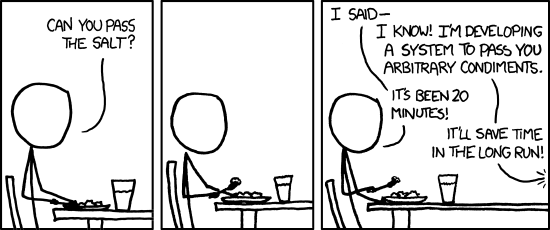
\includegraphics[width=0.9\linewidth]{images/xkcd-the_general_problem} 

}

\caption{The General Problem, by xkcd.}\label{fig:gneral-problem}
\end{figure}

The xkcd cartoon alludes to a common aspiration of programmers: to solve
a frequently-occurring problem \emph{in general} so that we don't have
to keep on devising solutions specific for each case. In R and in most
other programming languages, \emph{functions} are one of the important
tools for solving problems in a general manner. In this Chapter we take
a close look at how functions work in R. Along the way we'll learn about
environments and scoping, receiving input from the user, and a few more
built-in R-functions.

\newpage

\section{Motivation for Functions}\label{motivation-for-functions}

\index{function}

Suppose you have the job of printing out the word ``Kansas'' to the
console four times, each time on a new line. The code for this is easy
enough:

\begin{Shaded}
\begin{Highlighting}[]
\KeywordTok{cat}\NormalTok{(}\StringTok{"Kansas}\CharTok{\textbackslash{}n}\StringTok{"}\NormalTok{)}
\end{Highlighting}
\end{Shaded}

\begin{verbatim}
## Kansas
\end{verbatim}

\begin{Shaded}
\begin{Highlighting}[]
\KeywordTok{cat}\NormalTok{(}\StringTok{"Kansas}\CharTok{\textbackslash{}n}\StringTok{"}\NormalTok{)}
\end{Highlighting}
\end{Shaded}

\begin{verbatim}
## Kansas
\end{verbatim}

\begin{Shaded}
\begin{Highlighting}[]
\KeywordTok{cat}\NormalTok{(}\StringTok{"Kansas}\CharTok{\textbackslash{}n}\StringTok{"}\NormalTok{)}
\end{Highlighting}
\end{Shaded}

\begin{verbatim}
## Kansas
\end{verbatim}

\begin{Shaded}
\begin{Highlighting}[]
\KeywordTok{cat}\NormalTok{(}\StringTok{"Kansas}\CharTok{\textbackslash{}n}\StringTok{"}\NormalTok{)}
\end{Highlighting}
\end{Shaded}

\begin{verbatim}
## Kansas
\end{verbatim}

Now suppose that you have the job of printing out \emph{any given} word
to the console four times. You could of course, simply copy and paste
the above code to a new place in your R script and then change
``Kansas'' to whatever the desired word is. But that's an awful lot of
work.

You could cut down on the work a bit if you use a variable:

\begin{Shaded}
\begin{Highlighting}[]
\NormalTok{word <-}\StringTok{ "Kansas"}
\KeywordTok{cat}\NormalTok{(word, }\StringTok{"}\CharTok{\textbackslash{}n}\StringTok{"}\NormalTok{, }\DataTypeTok{sep =} \StringTok{""}\NormalTok{)}
\KeywordTok{cat}\NormalTok{(word, }\StringTok{"}\CharTok{\textbackslash{}n}\StringTok{"}\NormalTok{, }\DataTypeTok{sep =} \StringTok{""}\NormalTok{)}
\KeywordTok{cat}\NormalTok{(word, }\StringTok{"}\CharTok{\textbackslash{}n}\StringTok{"}\NormalTok{, }\DataTypeTok{sep =} \StringTok{""}\NormalTok{)}
\KeywordTok{cat}\NormalTok{(word, }\StringTok{"}\CharTok{\textbackslash{}n}\StringTok{"}\NormalTok{, }\DataTypeTok{sep =} \StringTok{""}\NormalTok{)}
\end{Highlighting}
\end{Shaded}

The advantage of this approach is that, after you copy and paste you
only have to make one change, i.e.: substitute the desired word in place
of ``Kansas'' in the assignment to the variable \texttt{word}.

If you were writing a program that involved many four-line print-outs of
various words, then you could carry on this way quite a while, producing
many similar five-line snippets of printing-code throughout your
program.

But suppose that it occurs to you one day: maybe you don't really need
five lines of code. What if \texttt{cat()} supports ``vector in, vector
out''? If so then we could take advantage of vectorization to obviate
the need to repeated calls to `cat().

We could try:

\begin{Shaded}
\begin{Highlighting}[]
\NormalTok{fourWords <-}\StringTok{ }\KeywordTok{rep}\NormalTok{(}\StringTok{"Kansas"}\NormalTok{, }\DecValTok{4}\NormalTok{)}
\KeywordTok{cat}\NormalTok{(fourWords, }\StringTok{"}\CharTok{\textbackslash{}n}\StringTok{"}\NormalTok{)}
\end{Highlighting}
\end{Shaded}

\begin{verbatim}
## Kansas Kansas Kansas Kansas
\end{verbatim}

That just repeats ``Kansas'' four times, with the default space between
in each one---then newline is appended. So we need a newline along with
each instance of Kansas.

So instead we try:

\begin{Shaded}
\begin{Highlighting}[]
\NormalTok{fourWords <-}\StringTok{ }\KeywordTok{rep}\NormalTok{(}\StringTok{"Kansas}\CharTok{\textbackslash{}n}\StringTok{"}\NormalTok{, }\DecValTok{4}\NormalTok{)}
\KeywordTok{cat}\NormalTok{(fourWords)}
\end{Highlighting}
\end{Shaded}

\begin{verbatim}
## Kansas
##  Kansas
##  Kansas
##  Kansas
\end{verbatim}

Not quite what we wanted: \texttt{cat()} inserts the default space at
the end of each instance of \texttt{Kansas\textbackslash{}n}, resulting
in the indentation of lines, 2, 3 and 4.

No problem---let's just set the separation to the empty string ``'':

\begin{Shaded}
\begin{Highlighting}[]
\NormalTok{fourWords <-}\StringTok{ }\KeywordTok{rep}\NormalTok{(}\StringTok{"Kansas}\CharTok{\textbackslash{}n}\StringTok{"}\NormalTok{, }\DecValTok{4}\NormalTok{)}
\KeywordTok{cat}\NormalTok{(fourWords, }\DataTypeTok{sep =} \StringTok{""}\NormalTok{)}
\end{Highlighting}
\end{Shaded}

\begin{verbatim}
## Kansas
## Kansas
## Kansas
## Kansas
\end{verbatim}

Success at last!

If you wanted to implement this new idea throughout your program, you
would have to search through the program for the many five-line snippets
you created previously, replacing each one of them with the appropriate
version of your clever one-liner. Not only is this a lot of work, it's
also quite error-prone: you could miss or more of the snippets along the
way, or on some occasion fail to modify the word within the one-liner to
have the value you need at that point.

Accordingly programmers try, as much as possible, to solve problems in a
\emph{general} way and to implement that general solution in \emph{one
place} in their program. Then they call upon that solution in the many
different locations where the solution might be required.

Functions are one way in which programmers accomplish this. The
following is a function that will print any given word four times, once
on each line:

\begin{Shaded}
\begin{Highlighting}[]
\NormalTok{catFourTimes <-}\StringTok{ }\NormalTok{function(word) \{}
  \NormalTok{wordWithNewline <-}\StringTok{ }\KeywordTok{paste}\NormalTok{(word, }\StringTok{"}\CharTok{\textbackslash{}n}\StringTok{"}\NormalTok{, }\DataTypeTok{sep =} \StringTok{""}\NormalTok{)}
  \KeywordTok{cat}\NormalTok{(}\KeywordTok{rep}\NormalTok{(wordWithNewline, }\DecValTok{4}\NormalTok{), }\DataTypeTok{sep =} \StringTok{""}\NormalTok{)}
\NormalTok{\}}
\end{Highlighting}
\end{Shaded}

Let's see the function in use:

\begin{Shaded}
\begin{Highlighting}[]
\KeywordTok{catFourTimes}\NormalTok{(}\StringTok{"Kansas"}\NormalTok{)}
\end{Highlighting}
\end{Shaded}

\begin{verbatim}
## Kansas
## Kansas
## Kansas
## Kansas
\end{verbatim}

It works like a charm! What's more, once we get to thinking in terms of
general solutions, we realize that we might just as well have our
function print not only any given word, but print it any given number of
times. So instead of \texttt{catFourTimes()} we might actually use the
following:

\begin{Shaded}
\begin{Highlighting}[]
\NormalTok{manyCat <-}\StringTok{ }\NormalTok{function(word, n) \{}
  \NormalTok{wordWithNewline <-}\StringTok{ }\KeywordTok{paste}\NormalTok{(word, }\StringTok{"}\CharTok{\textbackslash{}n}\StringTok{"}\NormalTok{, }\DataTypeTok{sep =} \StringTok{""}\NormalTok{)}
  \NormalTok{lines <-}\StringTok{ }\KeywordTok{rep}\NormalTok{(wordWithNewline, }\DataTypeTok{times =} \NormalTok{n)}
  \KeywordTok{cat}\NormalTok{(lines, }\DataTypeTok{sep =} \StringTok{""}\NormalTok{)}
\NormalTok{\}}
\end{Highlighting}
\end{Shaded}

Does it work? Let's see:

\begin{Shaded}
\begin{Highlighting}[]
\KeywordTok{manyCat}\NormalTok{(}\StringTok{"Kansas"}\NormalTok{, }\DecValTok{5}\NormalTok{)}
\end{Highlighting}
\end{Shaded}

\begin{verbatim}
## Kansas
## Kansas
## Kansas
## Kansas
## Kansas
\end{verbatim}

Yes indeed!

Let's consider the advantages of writing functions:

\begin{itemize}
\tightlist
\item
  Functions allow us to re-use code, rather than repeating the code
  throughout our program.
\item
  The more generally the functions solves the problem, the varied are
  the situations in which the function may be re-used.
\item
  If we have to change our our approach to the problem---because our
  original solution was flawed or if there is a need to add new features
  to our solution, or for any other reason---then we only have to
  implement the necessary change in the definition of our function,
  rather than in the many places in the program where the function is
  actually used.
\end{itemize}

There is a well-known principle in computer programming called DRY,
which is an acronym for \emph{``Don't Repeat Yourself.''}
\index{DRY}Computer code is said to be DRY when general solutions are
defined in one place but are usable in many places, and when information
needed in many places is defined authoritatively in one place. As a
rule, DRY code is easy to develop, debug, read and maintain. The more
you get into the habit of expressing solutions to problems in terms of
functions, the ``drier'' your code will be.

\section{Function Syntax}\label{function-syntax}

\texttt{function} is the reserved word in R that permits us to define
functions. The general form of a function definition is as follows:

\begin{Shaded}
\begin{Highlighting}[]
\NormalTok{functionName <-}\StringTok{ }\NormalTok{function(parameter, parameter, ...) \{}
  \NormalTok{Body of the Function ...}
\NormalTok{\}}
\end{Highlighting}
\end{Shaded}

\texttt{fucntionName} is the variable that will refer to the function
you define. Like any other identifier, it can contain letters, numbers,
the dot and the underscore character, but is not permitted to begin with
the dot followed by a number.

After the \texttt{function} reserved word we see a pair of matching
parentheses. They contain the \emph{parameters}\index{parameter} of the
function, which will be passed into the function as variables referred
to by the parameter names.

The \emph{body} \index{body of a function} of the function consists of
one or more expressions that do the work of the function. Note that the
body is enclosed with curly braces. This is only necessary, though, if
the body consists of more than one expression. If the body had only one
expression then that expression could appear without the braces, like
this:

\begin{Shaded}
\begin{Highlighting}[]
\NormalTok{add3 <-}\StringTok{ }\NormalTok{function(x) x}\DecValTok{+3}
\KeywordTok{add3}\NormalTok{(}\DataTypeTok{x =} \DecValTok{5}\NormalTok{)}
\end{Highlighting}
\end{Shaded}

\begin{verbatim}
## [1] 8
\end{verbatim}

\begin{Shaded}
\begin{Highlighting}[]
\KeywordTok{add3}\NormalTok{(-}\DecValTok{7}\NormalTok{)}
\end{Highlighting}
\end{Shaded}

\begin{verbatim}
## [1] -4
\end{verbatim}

In the \texttt{add3()} function above, \texttt{x} was a parameter. When
the function is called the parameter is assigned a particular value
called an \emph{argument}.\index{argument} We see that \texttt{add3()}
was called twice, once with an argument of 3 and again with an argument
of -7. If the parameter is explicitly mentioned in the function call,
then an equal-sign \texttt{=} separates the parameter and the argument.
Note also that the parameter and \texttt{=} may be omitted if it is
clear what parameter the argument will be matched to. In the case of
\texttt{add3} there is only one parameter \texttt{x}, so R knows that
any value provided within the parentheses is to be assigned to
\texttt{x}. R also knows to refer to the order of parameters within the
function's definition to determine which arguments go with which
parameters. Thus, the following calls do the same thing:

\begin{Shaded}
\begin{Highlighting}[]
\KeywordTok{manyCat}\NormalTok{(}\DataTypeTok{word =} \StringTok{"Hello"}\NormalTok{, }\DataTypeTok{n =} \DecValTok{4}\NormalTok{)}
\KeywordTok{manyCat}\NormalTok{(}\DataTypeTok{word =} \StringTok{"Hello"}\NormalTok{, }\DecValTok{4}\NormalTok{)}
\KeywordTok{manyCat}\NormalTok{(}\StringTok{"Hello"}\NormalTok{, }\DataTypeTok{n =} \DecValTok{4}\NormalTok{)}
\KeywordTok{manyCat}\NormalTok{(}\StringTok{"Hello"}\NormalTok{, }\DecValTok{4}\NormalTok{)}
\KeywordTok{manyCat}\NormalTok{(}\DataTypeTok{n =} \DecValTok{4}\NormalTok{, }\DataTypeTok{word =} \StringTok{"Hello"}\NormalTok{)}
\end{Highlighting}
\end{Shaded}

On the other hand, the following would produce an error:

\begin{Shaded}
\begin{Highlighting}[]
\KeywordTok{manyCat}\NormalTok{(}\DecValTok{4}\NormalTok{, }\StringTok{"Hello"}\NormalTok{)}
\end{Highlighting}
\end{Shaded}

\begin{verbatim}
## NAs introduced by coercion
## Error in rep(wordWithNewline, times = n) :
## invalid 'times' argument
\end{verbatim}

If you don't label your arguments with the parameters they are to match
to, then you must at least write them in the order in which the
parameters appear in the definition of the function.

In the definition of functions and in all calls to functions, commas
must separate arguments. Thus the following would produce an error:

\begin{Shaded}
\begin{Highlighting}[]
\KeywordTok{manyCat}\NormalTok{(}\StringTok{"Hello"} \DecValTok{4}\NormalTok{)}
\end{Highlighting}
\end{Shaded}

\begin{verbatim}
## Error: unexpected numeric constant in "manyCat("Hello" 4"
\end{verbatim}

If R cannot match all your arguments to a parameter it will throw an
error;

\begin{Shaded}
\begin{Highlighting}[]
\KeywordTok{manyCat}\NormalTok{(}\StringTok{"Hello"}\NormalTok{, }\DecValTok{4}\NormalTok{, }\DecValTok{7}\NormalTok{)}
\end{Highlighting}
\end{Shaded}

\begin{verbatim}
## Error in manyCat("Hello", 4, 7) : unused argument (7)
\end{verbatim}

You will have noticed by now that parentheses are essential when using a
function. What would happen if we typed just the function's name itself?
Give it a try:

\begin{Shaded}
\begin{Highlighting}[]
\NormalTok{manyCat}
\end{Highlighting}
\end{Shaded}

\begin{verbatim}
## function(word, n) {
##   wordWithNewline <- paste(word, "\n", sep = "")
##   lines <- rep(wordWithNewline, times = n)
##   cat(lines, sep = "")
## }
\end{verbatim}

What's printed to the screen is the code that defines the function. The
function itself is not called.

\section{What a Function Returns}\label{what-a-function-returns}

In this section we learn about return-values of functions.

\subsection{The Final Expression
Evaluated}\label{the-final-expression-evaluated}

Let's write a small function to raise a number to a power:\footnote{I
  know, I know---R already has the exponentiation operator. We just need
  an example to work with, here.}

\begin{Shaded}
\begin{Highlighting}[]
\NormalTok{pow <-}\StringTok{ }\NormalTok{function(x,y) \{}
  \NormalTok{x^y}
\NormalTok{\}}
\end{Highlighting}
\end{Shaded}

Check to see that it works:

\begin{Shaded}
\begin{Highlighting}[]
\KeywordTok{pow}\NormalTok{(}\DecValTok{2}\NormalTok{,}\DecValTok{3}\NormalTok{)}
\end{Highlighting}
\end{Shaded}

\begin{verbatim}
## [1] 8
\end{verbatim}

All seems well.

If we like we can assign the result of \texttt{pow()} to some variable,
for use later on:

\begin{Shaded}
\begin{Highlighting}[]
\NormalTok{a <-}\StringTok{ }\KeywordTok{pow}\NormalTok{(}\DecValTok{2}\NormalTok{,}\DecValTok{4}\NormalTok{)}
\KeywordTok{cat}\NormalTok{(}\StringTok{"I have"}\NormalTok{, a, }\StringTok{"cats."}\NormalTok{)}
\end{Highlighting}
\end{Shaded}

\begin{verbatim}
## I have 16 cats.
\end{verbatim}

In computer programming parlance, \texttt{pow(x,\ y)} is said to
\emph{return}\index{return} the numerical value \texttt{x\^{}y}:
\texttt{pow(2,3)} returns 8, \texttt{pow(2,4)} returns 16, and so on.

In R, what a function returns is: \emph{the value of the final
expression that it evaluates}. You can see this principle at work in the
following example:

\begin{Shaded}
\begin{Highlighting}[]
\NormalTok{f <-}\StringTok{ }\NormalTok{function(x) \{}
  \DecValTok{2}\NormalTok{*x +}\StringTok{ }\DecValTok{3}
  \DecValTok{45}
  \StringTok{"hello"}
  \NormalTok{x^}\DecValTok{2}
\NormalTok{\}}

\KeywordTok{f}\NormalTok{(}\DecValTok{4}\NormalTok{)}
\end{Highlighting}
\end{Shaded}

\begin{verbatim}
## [1] 16
\end{verbatim}

We put in 4 as the argument for the parameter \texttt{x}, but:

\begin{itemize}
\tightlist
\item
  we did not get back 11 (\(2 \times 4 +3\)),
\item
  nor did we get back 45,
\item
  nor did we get back the string ``hello''.
\end{itemize}

When \texttt{f()} was called, R evaluated all of the expressions in its
body, but returned only the value of the final expression it evaluated:
\(4^2 = 16\).

\subsection{\texorpdfstring{The \texttt{return()}
Function}{The return() Function}}\label{the-return-function}

R does have a special function to force a function to cease evaluation
at a specific point. Its name, unsurprisingly, is
\texttt{return()}\index{R-functions!return()@\texttt{return()}}. Here is
an example:

\begin{Shaded}
\begin{Highlighting}[]
\NormalTok{g <-}\StringTok{ }\NormalTok{function(x) \{}
  \NormalTok{val <-}\StringTok{ }\DecValTok{3}\NormalTok{*x +}\DecValTok{7}
  \KeywordTok{return}\NormalTok{(val)}
  \StringTok{"Hello!"}
\NormalTok{\}}

\KeywordTok{g}\NormalTok{(}\DecValTok{1}\NormalTok{)}
\end{Highlighting}
\end{Shaded}

\begin{verbatim}
## [1] 10
\end{verbatim}

We get \(3*1+7 = 10\), but we don't get ``Hello!''. After returning the
10, the function stopped evaluating expressions: hence it never even
bothered to evaluate ``Hello'', much less to display it in the
console.\footnote{You might wonder why anyone would write a function
  that contains expressions after a call to \texttt{return()}. We'll
  learn why in Chapter \ref{flow}.}

It follows that it does not matter whether or not you wrap the final
expression of a function in \texttt{return()}. The following two
functions do exactly the same thing:

\begin{Shaded}
\begin{Highlighting}[]
\NormalTok{f1 <-}\StringTok{ }\NormalTok{function(x) x^}\DecValTok{2}
\NormalTok{f2 <-}\StringTok{ }\NormalTok{function(x) }\KeywordTok{return}\NormalTok{(x^}\DecValTok{2}\NormalTok{)}
\end{Highlighting}
\end{Shaded}

Some people---especially those who are familiar with other programming
languages where return statements are required---like to wrap the final
expression in \texttt{return()}, simply as a matter of clarity.

\subsection{\texorpdfstring{Writing a ``Talky''
Function}{Writing a Talky Function}}\label{writing-a-talky-function}

Suppose that you would like your function to raise a number to a power,
returning the answer to the user, but you also want it to print out a
message to the console. You might try writing your function like this:

\begin{Shaded}
\begin{Highlighting}[]
\NormalTok{talkySquare <-}\StringTok{ }\NormalTok{function(x) \{}
  \NormalTok{result <-}\StringTok{ }\NormalTok{x^}\DecValTok{2}
  \NormalTok{result}
  \KeywordTok{cat}\NormalTok{(}\StringTok{"The square of "}\NormalTok{, x, }\StringTok{" is:  "}\NormalTok{, result, }\StringTok{".}\CharTok{\textbackslash{}n}\StringTok{"}\NormalTok{, }\DataTypeTok{sep =} \StringTok{""}\NormalTok{)}
\NormalTok{\}}
\end{Highlighting}
\end{Shaded}

We try it out:

\begin{Shaded}
\begin{Highlighting}[]
\KeywordTok{talkySquare}\NormalTok{(}\DecValTok{4}\NormalTok{)}
\end{Highlighting}
\end{Shaded}

\begin{verbatim}
## The square of 4 is:  16.
\end{verbatim}

All seems well. But what if we want to save the result in a variable, so
that we could perhaps add a number to it later? Something like this,
perhaps:

\begin{Shaded}
\begin{Highlighting}[]
\NormalTok{a <-}\StringTok{ }\KeywordTok{talkySquare}\NormalTok{(}\DecValTok{4}\NormalTok{)}
\end{Highlighting}
\end{Shaded}

\begin{verbatim}
## The square of 4 is:  16.
\end{verbatim}

\begin{Shaded}
\begin{Highlighting}[]
\NormalTok{a +}\StringTok{ }\DecValTok{4}
\end{Highlighting}
\end{Shaded}

\begin{verbatim}
## numeric(0)
\end{verbatim}

The results don't really make sense. What happened, of course is that R
dutifully returned the value of the final expression in the function's
body---the result of the \texttt{cat()} call, not the value of the
variable \texttt{result}. If we want both the print-out \emph{and} the
square to be returned, the we have to write our functions like this:

\begin{Shaded}
\begin{Highlighting}[]
\NormalTok{talkySquare <-}\StringTok{ }\NormalTok{function(x) \{}
  \NormalTok{result <-}\StringTok{ }\NormalTok{x^}\DecValTok{2}
  \KeywordTok{cat}\NormalTok{(}\StringTok{"The square of "}\NormalTok{, x, }\StringTok{" is:  "}\NormalTok{, result, }\StringTok{".}\CharTok{\textbackslash{}n}\StringTok{"}\NormalTok{, }\DataTypeTok{sep =} \StringTok{""}\NormalTok{)}
  \NormalTok{result}
\NormalTok{\}}
\end{Highlighting}
\end{Shaded}

This works out as expected:

\begin{Shaded}
\begin{Highlighting}[]
\NormalTok{a <-}\StringTok{ }\KeywordTok{talkySquare}\NormalTok{(}\DecValTok{4}\NormalTok{)}
\end{Highlighting}
\end{Shaded}

\begin{verbatim}
## The square of 4 is:  16.
\end{verbatim}

\begin{Shaded}
\begin{Highlighting}[]
\NormalTok{a +}\StringTok{ }\DecValTok{4}
\end{Highlighting}
\end{Shaded}

\begin{verbatim}
## [1] 20
\end{verbatim}

Well, maybe it doesn't work \emph{exactly} as we would like. It would
nice if the function would talk to us only when we ask for the results
in the console, not when we are simply assigning the results to a
variable for later use. In Chapter \ref{flow} we will learn how to make
our talky function keep quiet when we prefer silence.

\subsection{\texorpdfstring{The \texttt{print()}
Function}{The print() Function}}\label{the-print-function}

Consider the following function:

\begin{Shaded}
\begin{Highlighting}[]
\NormalTok{grumpySquare <-}\StringTok{ }\NormalTok{function(x) \{}
  \StringTok{"OK, OK, I'm getting to it ... "}
  \NormalTok{x^}\DecValTok{2}
\NormalTok{\}}
\end{Highlighting}
\end{Shaded}

We know by now not to expect to see the grumpy message:

\begin{Shaded}
\begin{Highlighting}[]
\KeywordTok{grumpySquare}\NormalTok{(}\DecValTok{4}\NormalTok{)}
\end{Highlighting}
\end{Shaded}

\begin{verbatim}
## [1] 16
\end{verbatim}

If we want to see the message, we could wrap it in \texttt{cat()}.
Another possibility is to use the
\texttt{print()}\index{R-functions!print()@\texttt{print()}} function:

\begin{Shaded}
\begin{Highlighting}[]
\NormalTok{grumpySquare <-}\StringTok{ }\NormalTok{function(x) \{}
  \KeywordTok{print}\NormalTok{(}\StringTok{"OK, OK, I'm getting to it ... "}\NormalTok{)}
  \NormalTok{x^}\DecValTok{2}
\NormalTok{\}}
\KeywordTok{grumpySquare}\NormalTok{(}\DecValTok{4}\NormalTok{)}
\end{Highlighting}
\end{Shaded}

\begin{verbatim}
## [1] "OK, OK, I'm getting to it ... "
\end{verbatim}

\begin{verbatim}
## [1] 16
\end{verbatim}

When R executes a call to \texttt{print()} it is forced to print
something out to the console, even if it is in the midst of evaluating
expressions in a function. The \texttt{print}-statement is not involved
in what the function returns---that's all up to the expression
\texttt{x\^{}2}---but it does cause a result \emph{outside of the
function itself}. Any external result produced by a function (other than
what the function returns) is called a \emph{side-effect}
\index{side-effect}of the function. \texttt{cat()} and \texttt{print()}
are examples of functions that, when called inside of some other
function, produce side-effects.

You should know that in R you have been calling the \texttt{print()}
function quite a bit, without even knowing it. Consider the following
line of code:

\begin{Shaded}
\begin{Highlighting}[]
\DecValTok{2+2}
\end{Highlighting}
\end{Shaded}

\begin{verbatim}
## [1] 4
\end{verbatim}

R evaluates the expression \texttt{2+2}, arriving at the value 4. But
what makes the \texttt{4} appear on our console? Behind the scenes, R
actually evaluated the expression

\begin{quote}
\texttt{print(2+2)}
\end{quote}

That's what got the 4 into the console!

At this point we don't use \texttt{print()} explicitly very much---we
just rely on R to call it for us when we are evaluating expressions at
the console. Later on we will find that it has other uses.\footnote{R is
  one of very few major programming languages that engage in
  behind-the-scenes calls to a print function. In many other languages
  you have to call its print-function explicitly if you want the value
  of an expression to be displayed.}

\section{More About Arguments}\label{more-about-arguments}

\subsection{Default Arguments}\label{default-arguments}

Sometime around the year 1400CE, the South Indian mathematician Madhava
discovered the following infinite-series formula for \(\pi\), the ratio
of the circumference to the diameter of a circle:

\[\pi = \frac{4}{1} - \frac{4}{3} + \frac{4}{5} - \frac{4}{7} +\frac{4}{9} - \cdots\]
The numerator of each fraction is always 4. The denominators are the odd
numbers 1, 3, 5, and so on. The fractions alternate between positive and
negative. The idea is that the further you go out in the series, the
closer the sum of the fractions will be to \(\pi\). No matter how close
you want to get to \(\pi\), you can get that close by adding up
sufficiently many of the fractions.

In mathematics courses we learn to write the sum like this:

\[\pi = \sum_{k=1}^{k=\infty} (-1)^{k+1}\frac{4}{2k-1}.\] Here's how the
mathematical notation works:

\begin{itemize}
\tightlist
\item
  The \(\Sigma\) sign stands for ``sum'': it means that we plan to add
  up a lot of terms.
\item
  The expression \((-1)^k\frac{4}{2k-1}\) after the sum-sign stands for
  all of the terms that will be added up to make the infinite series.
\item
  Underneath the sum-sign, \(k=1\) says that in the expression after the
  sum sign we will start by letting \(k\) be 1.
\item
  If we let \(k=1\), then the expression becomes
  \[(-1)^2\frac{4}{2 \cdot 1 -1} = \frac{4}{1} = 4,\] the first term in
  the series.
\item
  If we let \(k=2\), then the expression becomes
  \[(-1)^3\frac{4}{2 \cdot 2 -1} = -\frac{4}{3}\] the second term in the
  series.
\item
  If we let \(k=3\), then the expression becomes
  \[(-1)^4\frac{4}{2 \cdot 3 -1} = \frac{4}{5}\] the third term in the
  series.
\item
  The \(k = \infty\) above the sum-sign says that we are to keep on
  going like this, increasing \(k\) by 1 every time, without stopping.
\item
  In this way we get the entire infinite series.
\end{itemize}

What Madhava discovered was that if you \emph{do} stop after some large
number of terms, then the sum of the terms you have constructed will be
close to \(\pi\). The more terms you add up before stopping, the closer
to \(\pi\) you will get.

Let's write a function to compute the sum of the first \(n\) terms of
the series, where \(n\) can be any value we choose.

\begin{Shaded}
\begin{Highlighting}[]
\CommentTok{# function to approximate pi with Madhava's series}
\CommentTok{# (sum the first n terms of the series)}
\NormalTok{madhavaPI <-}\StringTok{ }\NormalTok{function(n) \{}
  \CommentTok{# make a vector of all of the k's we need:}
  \NormalTok{k <-}\StringTok{ }\DecValTok{1}\NormalTok{:n}
  \CommentTok{# make a vector of the first n terms of the sum:}
  \NormalTok{terms <-}\StringTok{ }\NormalTok{(-}\DecValTok{1}\NormalTok{)^(k}\DecValTok{+1}\NormalTok{)*}\DecValTok{4}\NormalTok{/(}\DecValTok{2}\NormalTok{*k}\DecValTok{-1}\NormalTok{)}
  \CommentTok{# return the sum of the terms:}
  \KeywordTok{sum}\NormalTok{(terms)}
\NormalTok{\}}
\end{Highlighting}
\end{Shaded}

R's vectorization capabilities make it easy to write the code; in fact,
the code is essentially a copy of the sum-formula.

Note also the presence of \emph{comments} in the code above. Anything
that appears on a line after the pound-sign \texttt{\#} will be ignored
by R. We therefore use the \texttt{\#}-sign to insert ordinary-language
comments into our code in order to explain to others (and to ourselves
when we look at the code much later) what we are doing and why we are
doing it.

Let's try it out by adding the first million terms of the series:

\begin{Shaded}
\begin{Highlighting}[]
\KeywordTok{madhavaPI}\NormalTok{(}\DecValTok{1000000}\NormalTok{)}
\end{Highlighting}
\end{Shaded}

\begin{verbatim}
## [1] 3.141592
\end{verbatim}

How close is this to \(\pi\)? R has a built-in constant
\texttt{pi}\index{R-constants!pi@\texttt{pi}} that will tell us:

\begin{Shaded}
\begin{Highlighting}[]
\NormalTok{pi}
\end{Highlighting}
\end{Shaded}

\begin{verbatim}
## [1] 3.141593
\end{verbatim}

Madhava's approximation was pretty close, although we did have to add up
quite a few terms!

The \texttt{madhavaPI()} function has a parameter \texttt{n} that stands
for the number of terms we want to add up. If we don't provide a value
for \texttt{n}, then there will be an error:

\begin{Shaded}
\begin{Highlighting}[]
\KeywordTok{madhavaPI}\NormalTok{()}
\end{Highlighting}
\end{Shaded}

\begin{verbatim}
## Error in madhavaPI() : argument "n" is missing, with no default
\end{verbatim}

There is a way, though, to allow a user to avoid providing a value for
\texttt{n}. We simply provide a \emph{default
value}\index{default value} for it, like this:

\begin{Shaded}
\begin{Highlighting}[]
\NormalTok{madhavaPI <-}\StringTok{ }\NormalTok{function(}\DataTypeTok{n =} \DecValTok{1000000}\NormalTok{) \{}
  \NormalTok{k <-}\StringTok{ }\DecValTok{1}\NormalTok{:n}
  \NormalTok{terms <-}\StringTok{ }\NormalTok{(-}\DecValTok{1}\NormalTok{)^(k}\DecValTok{+1}\NormalTok{)*}\DecValTok{4}\NormalTok{/(}\DecValTok{2}\NormalTok{*k}\DecValTok{-1}\NormalTok{)}
  \KeywordTok{sum}\NormalTok{(terms)}
\NormalTok{\}}
\end{Highlighting}
\end{Shaded}

If the user provides his or her own value, it will \emph{override} the
default:

\begin{Shaded}
\begin{Highlighting}[]
\KeywordTok{madhavaPI}\NormalTok{(}\DecValTok{100}\NormalTok{)}
\end{Highlighting}
\end{Shaded}

\begin{verbatim}
## [1] 3.131593
\end{verbatim}

On the other hand, if the user provides nothing then the function sums
the first million terms.

If you are writing a function for which some of the parameters will
often be assigned particular values, it would be a kindness to your
users to write in these common values as defaults.

\hypertarget{argument-matching}{\subsection{Argument-Matching}\label{argument-matching}}

Sometimes you will see functions in R that provide what appears to be a
\emph{vector} of default values. You'll see this in the following
example, which concerns a function that uses a named vector to report
the favorite color of each of the major groups of inhabitants of the
Land of Oz.

\begin{Shaded}
\begin{Highlighting}[]
\NormalTok{inhabitants <-}\StringTok{ }\KeywordTok{c}\NormalTok{(}\StringTok{"Munchkin"}\NormalTok{, }\StringTok{"Winkie"}\NormalTok{, }
            \StringTok{"Quadling"}\NormalTok{, }\StringTok{"Gillikin"}\NormalTok{)}
\NormalTok{favColor <-}\StringTok{ }\KeywordTok{c}\NormalTok{(}\StringTok{"blue"}\NormalTok{, }\StringTok{"yellow"}\NormalTok{, }\StringTok{"red"}\NormalTok{, }\StringTok{"purple"}\NormalTok{)}
\KeywordTok{names}\NormalTok{(favColor) <-}\StringTok{ }\NormalTok{inhabitants}

\NormalTok{favColorReport <-}\StringTok{ }\NormalTok{function(}\DataTypeTok{inhabitant =} \NormalTok{inhabitants) \{}
  \NormalTok{x <-}\StringTok{ }\KeywordTok{match.arg}\NormalTok{(inhabitant)}
  \KeywordTok{cat}\NormalTok{(favColor[x],}\StringTok{"}\CharTok{\textbackslash{}n}\StringTok{"}\NormalTok{)}
\NormalTok{\}}
\end{Highlighting}
\end{Shaded}

Here are a couple of sample calls:

\begin{Shaded}
\begin{Highlighting}[]
\KeywordTok{favColorReport}\NormalTok{(}\StringTok{"Winkie"}\NormalTok{)}
\end{Highlighting}
\end{Shaded}

\begin{verbatim}
## yellow
\end{verbatim}

\begin{Shaded}
\begin{Highlighting}[]
\KeywordTok{favColorReport}\NormalTok{(}\StringTok{"Quadling"}\NormalTok{)}
\end{Highlighting}
\end{Shaded}

\begin{verbatim}
## red
\end{verbatim}

It might get tiresome to type out the full name of each group of
inhabitants. What would happen if we got a bit lazy?

\begin{Shaded}
\begin{Highlighting}[]
\KeywordTok{favColorReport}\NormalTok{(}\StringTok{"Win"}\NormalTok{)}
\end{Highlighting}
\end{Shaded}

\begin{verbatim}
## yellow
\end{verbatim}

\begin{Shaded}
\begin{Highlighting}[]
\KeywordTok{favColorReport}\NormalTok{(}\StringTok{"Wi"}\NormalTok{)}
\end{Highlighting}
\end{Shaded}

\begin{verbatim}
## yellow
\end{verbatim}

\begin{Shaded}
\begin{Highlighting}[]
\KeywordTok{favColorReport}\NormalTok{(}\StringTok{"W"}\NormalTok{)}
\end{Highlighting}
\end{Shaded}

\begin{verbatim}
## yellow
\end{verbatim}

\begin{Shaded}
\begin{Highlighting}[]
\KeywordTok{favColorReport}\NormalTok{(}\StringTok{"Qua"}\NormalTok{)}
\end{Highlighting}
\end{Shaded}

\begin{verbatim}
## red
\end{verbatim}

\begin{Shaded}
\begin{Highlighting}[]
\KeywordTok{favColorReport}\NormalTok{(}\StringTok{"Gil"}\NormalTok{)}
\end{Highlighting}
\end{Shaded}

\begin{verbatim}
## purple
\end{verbatim}

The key to this behavior is two-fold:

\begin{itemize}
\tightlist
\item
  The vector \texttt{inhabitants} was set as the ``default value'' of
  the parameter \texttt{inhabitant}.
\item
  We called the
  \texttt{match.arg()}\index{R-functions!match.arg()@\texttt{match.arg()}}
  function, which found the element of \texttt{inhabitants} that matched
  what the user actually submitted for the parameter
  \texttt{inhabitant}. This element was then assigned to \texttt{x}, and
  we used \texttt{x} to report the desired color.
\end{itemize}

Sometimes when you look at R-help you'll see the default value for a
parameter set as a vector---usually a character-vector, as in our
example. Most likely what is going on is that somewhere inside the
function R will attempt to match the argument you provide with one of
the elements of that ``default'' vector. When a function is written in
this way, the possible parameters can have quite long names but the user
doesn't have to type them in all the way, as long as the user types
enough characters to pick out uniquely an element of the default vector.

The matching is done by exact match of initial characters. For example,
it won't do for me to enter:

\begin{Shaded}
\begin{Highlighting}[]
\KeywordTok{favColorReport}\NormalTok{(}\StringTok{"w"}\NormalTok{)  }\CommentTok{# wants Winkies, but using lower-case w}
\end{Highlighting}
\end{Shaded}

\begin{verbatim}
## Error in match.arg(inhabitant) : 'arg' should be one of 
## “Munchkin”, “Winkie”, “Quadling”, “Gillikin”
\end{verbatim}

Note that the default vector isn't really a default \emph{value} for the
parameter. Its first element does, however, serve as the default value:

\begin{Shaded}
\begin{Highlighting}[]
\KeywordTok{favColorReport}\NormalTok{()  }\CommentTok{# defaults to "Munchkin"}
\end{Highlighting}
\end{Shaded}

\begin{verbatim}
## blue
\end{verbatim}

\section{Environments and Scope}\label{environments-and-scope}

\subsection{Environments and
Searching}\label{environments-and-searching}

In R an \emph{environment} is a particular kind of data structure that
helps the computer connect names to a value. An environment can be
thought of as a bag of names---names for vectors, functions, and all
sorts of objects---along with a way (provided automatically by the
computer) of getting from each name to the value that it represents. The
process that the computer follows in order to connect a name to a value
is called \emph{scoping}.\index{scoping} In R, as in many other computer
languages, environments are what makes scoping possible. In other words,
environments are how R figures out what the names in any piece of code
\emph{mean}.

R has a considerable number of environments---and environments can be
created and destroyed throughout the course of an R session---but at any
moment only one of them is \emph{active}. The \emph{active environment}
is \index{active environment}the first environment that R will examine
when it needs to look up a name in an expression.

The most familiar environment is the \emph{Global
Environment}---\index{global environment}the one that is active when you
are using R from the console. The names in the Global Environment, along
with descriptions of the objects to which they refer, are shown in the
\textbf{Environment} panel in the R Studio IDE. Alternatively, you see
the names in the Global Environment by using the
\texttt{ls()}\index{R-functions!ls()@\texttt{ls()}} function:

\begin{Shaded}
\begin{Highlighting}[]
\KeywordTok{ls}\NormalTok{()}
\end{Highlighting}
\end{Shaded}

You can remove all of the names from your Global Environment by pressing
the Broom icon in the IDE, or by using the
\texttt{rm()}function:\index{R-functions!rm()@\texttt{rm()}}

\begin{Shaded}
\begin{Highlighting}[]
\KeywordTok{rm}\NormalTok{(}\DataTypeTok{list =} \KeywordTok{ls}\NormalTok{())}
\end{Highlighting}
\end{Shaded}

As we mentioned previously, the Global Environment only one of many
environments that exist in R. The \texttt{search()}
function\index{R-functions!search()@\texttt{search()}} will show you a
number of other environments:

\begin{Shaded}
\begin{Highlighting}[]
\KeywordTok{search}\NormalTok{()}
\end{Highlighting}
\end{Shaded}

\begin{verbatim}
##  [1] ".GlobalEnv"             "package:R6"            
##  [3] "package:readr"          "package:tigerData"     
##  [5] "package:tigerstats"     "package:abd"           
##  [7] "package:mosaic"         "package:Matrix"        
##  [9] "package:dplyr"          "package:lattice"       
## [11] "package:nlme"           "package:TurtleGraphics"
## [13] "package:grid"           "package:ggplot2"       
## [15] "package:mosaicData"     "tools:rstudio"         
## [17] "package:stats"          "package:graphics"      
## [19] "package:grDevices"      "package:utils"         
## [21] "package:datasets"       "package:methods"       
## [23] "Autoloads"              "package:base"
\end{verbatim}

\texttt{search()} returns a character vector of names of environments.
The first element is the Global Environment itself. The second element
is an environment that is associated with last \emph{package} that R
loaded, the third is an environment associated with the next-to-last
package, and so on. Each item on the list is considered to be the
\emph{parent} of the environment \index{parent environment}that came
before it. Thus, the Global Environment has a parent environment, a
grandparent environment, and so on. The complete sequence of
environments is called the \emph{search path}. \index{search path}

Just as the Global Environment has names for objects, so also the
packages have names available for use. When you write code that contains
a name, R will search for that name: first in your Global Environment,
then in its parent environment---the environment of the last package
loaded---and so on until it reaches the final package on the list:
package \textbf{base}. If it can't find the name anywhere, then it will
throw an error, telling you that the object ``cannot be found.''

Let's try this with a few examples. First, define a (hopefully) new
variable:

\begin{Shaded}
\begin{Highlighting}[]
\NormalTok{quadlingColor <-}\StringTok{ "red"}
\end{Highlighting}
\end{Shaded}

Then use it in some code:

\begin{Shaded}
\begin{Highlighting}[]
\KeywordTok{cat}\NormalTok{(quadlingColor, }\StringTok{", white and blue}\CharTok{\textbackslash{}n}\StringTok{"}\NormalTok{, }\DataTypeTok{sep =}\StringTok{""}\NormalTok{)}
\end{Highlighting}
\end{Shaded}

\begin{verbatim}
## red, white and blue
\end{verbatim}

R was able to complete your request because:

\begin{itemize}
\tightlist
\item
  it found the name `quadlingColor on its search path;
\item
  it found the name \texttt{cat} on its search path (and found that it
  referred to the \texttt{cat()} function)
\end{itemize}

You can tell where R found these things:
\index{R-functions!find()@\texttt{find()}}

\begin{Shaded}
\begin{Highlighting}[]
\KeywordTok{find}\NormalTok{(}\StringTok{"quadlingColor"}\NormalTok{)}
\end{Highlighting}
\end{Shaded}

\begin{verbatim}
## [1] ".GlobalEnv"
\end{verbatim}

\begin{Shaded}
\begin{Highlighting}[]
\KeywordTok{find}\NormalTok{(}\StringTok{"cat"}\NormalTok{)}
\end{Highlighting}
\end{Shaded}

\begin{verbatim}
## [1] "package:base"
\end{verbatim}

R found \texttt{quadlingColor} in the first place it looked, whereas it
had to go all the way up to package \textbf{base} to find an object with
the name \texttt{cat} that looked like it was the name of a function.

What happens if the same name gets used in two different environments?
Let's investigate. First get a print of \texttt{cat()}:

\begin{Shaded}
\begin{Highlighting}[]
\NormalTok{cat}
\end{Highlighting}
\end{Shaded}

\begin{verbatim}
## function (..., file = "", sep = " ", fill = FALSE, labels = NULL, 
##     append = FALSE) 
## {
##     if (is.character(file)) 
##         if (file == "") 
##             file <- stdout()
##         else if (substring(file, 1L, 1L) == "|") {
##             file <- pipe(substring(file, 2L), "w")
##             on.exit(close(file))
##         }
##         else {
##             file <- file(file, ifelse(append, "a", "w"))
##             on.exit(close(file))
##         }
##     .Internal(cat(list(...), file, sep, fill, labels, append))
## }
## <bytecode: 0x10ca8e380>
## <environment: namespace:base>
\end{verbatim}

I got the definition of the \texttt{cat()} function, all the way up in
package \textbf{base}.

Now try:

\begin{Shaded}
\begin{Highlighting}[]
\KeywordTok{rep}\NormalTok{(cat, }\DataTypeTok{times =} \DecValTok{3}\NormalTok{)}
\end{Highlighting}
\end{Shaded}

\begin{verbatim}
## Error in rep(cat, times = 3) : 
##   attempt to replicate an object of type 'closure'
\end{verbatim}

I got an error! That's because the only reference R could find for
\texttt{cat} was to the function \texttt{cat()} in package
\textbf{base}, and since a function isn't a vector you can't repeat
it.\footnote{In R, almost all functions are called ``closures.''}

Next, define a variable named \texttt{cat}:

\begin{Shaded}
\begin{Highlighting}[]
\NormalTok{cat <-}\StringTok{ "Pippin"}
\end{Highlighting}
\end{Shaded}

At this point, we the identifier \texttt{cat} appears in at least two
environments:

\begin{itemize}
\tightlist
\item
  in the Global Environment, where is refers to the string ``Pippin'';
\item
  in the environment associated with package \textbf{base}, where is
  refers to the \texttt{cat()}-function.
\end{itemize}

We can verify the above assertions with \texttt{find()}:

\begin{Shaded}
\begin{Highlighting}[]
\KeywordTok{find}\NormalTok{(}\StringTok{"cat"}\NormalTok{)}
\end{Highlighting}
\end{Shaded}

\begin{verbatim}
## [1] ".GlobalEnv"   "package:base"
\end{verbatim}

Now try:

\begin{Shaded}
\begin{Highlighting}[]
\KeywordTok{rep}\NormalTok{(cat, }\DataTypeTok{times =} \DecValTok{3}\NormalTok{)}
\end{Highlighting}
\end{Shaded}

\begin{verbatim}
## [1] "Pippin" "Pippin" "Pippin"
\end{verbatim}

This time it worked! The reason is that R found a character-vector named
\texttt{cat} in the Global Environment.

Now try:

\begin{Shaded}
\begin{Highlighting}[]
\KeywordTok{cat}\NormalTok{(cat, }\StringTok{"is a cat}\CharTok{\textbackslash{}n}\StringTok{"}\NormalTok{)}
\end{Highlighting}
\end{Shaded}

\begin{verbatim}
## Pippin is a cat
\end{verbatim}

Wait a minute: why did this work? Doesn't the Global Environment come
before package \textbf{base} in the search path? Yes it does, but since
the first occurrence of \texttt{cat} was followed by an open parenthesis
R know to expect that it referred to a function. Hence it kept looking
along the search path for a function with the name \texttt{cat},
eventually finding our familiar \texttt{cat()} function in
\textbf{base}.

Well then, consider happens if we do this:

\begin{Shaded}
\begin{Highlighting}[]
\NormalTok{cat <-}\StringTok{ }\NormalTok{function(...) \{}
  \StringTok{"Meow!"}
\NormalTok{\}}
\end{Highlighting}
\end{Shaded}

We have defined a function \texttt{cat()} that returns ``Meow!'' no
matter what it is given as input.\footnote{The ellipses, which we will
  discuss further in Chapter \ref{lists}, allow the function to be
  passed any arguments at all---or even none.}

Now try again:

\begin{Shaded}
\begin{Highlighting}[]
\KeywordTok{cat}\NormalTok{(cat, }\StringTok{"is a cat}\CharTok{\textbackslash{}n}\StringTok{"}\NormalTok{)}
\end{Highlighting}
\end{Shaded}

\begin{verbatim}
## [1] "Meow!"
\end{verbatim}

Since the \texttt{cat()} we defined is a function in the Global
Environment---which comes before \textbf{base} in the search path---R
uses our \texttt{cat()} instead of the \textbf{base}'s \texttt{cat()}. R
programmers say that the \textbf{base} version of cat has been
\emph{masked}.

If I want to keep my \texttt{cat()} and still use the \textbf{base}
version of\texttt{cat()} as well, I can do that. In order to be sure of
getting a particular package's version of a function, put the name of
the package and then two semicolons before the function-name, like this:

\begin{Shaded}
\begin{Highlighting}[]
\NormalTok{base::}\KeywordTok{cat}\NormalTok{(}\StringTok{"This is the good ol' cat() we have been missing!"}\NormalTok{)}
\end{Highlighting}
\end{Shaded}

\begin{verbatim}
## This is the good ol' cat() we have been missing!
\end{verbatim}

But we don't like our \texttt{cat()} so very much: let's remove it:

\begin{Shaded}
\begin{Highlighting}[]
\KeywordTok{rm}\NormalTok{(cat)}
\end{Highlighting}
\end{Shaded}

The vector \texttt{cat} is removed as well by the previous command.

\subsection{Function Environments}\label{function-environments}

Let's summarize what we have learned so far:

\begin{itemize}
\tightlist
\item
  An environment is a collection of names associated with objects.
\item
  The Global Environment is the environment that is active when we are
  working from the console.
\item
  When R needs to look up a name, it consults a search path.
\item
  When we are in the Global Environment the search path starts there,
  and continues to:

  \begin{itemize}
  \tightlist
  \item
    the last package loaded (the parent environment),
  \item
    the package before that (the ``grandparent environment''),
  \item
    and so on \ldots{}
  \item
    \ldots{} up to package \textbf{base}.
  \end{itemize}
\item
  the first object of the right type having the given name that is found
  along the search path is the object to which R will associate the
  name.
\end{itemize}

Just as the Global Environment is a child of the last package loaded, so
the Global Environment can have children of its own. In fact a
child-environment is created whenever we define a function in the Global
Environment and then run it.

Consider the following code:

\begin{Shaded}
\begin{Highlighting}[]
\NormalTok{a <-}\StringTok{ }\DecValTok{10}
\NormalTok{b <-}\StringTok{ }\DecValTok{4}
\NormalTok{f <-}\StringTok{ }\NormalTok{function(x, y) \{}
  \NormalTok{a <-}\StringTok{ }\DecValTok{5}
  \KeywordTok{print}\NormalTok{(}\KeywordTok{ls}\NormalTok{())}
  \KeywordTok{cat}\NormalTok{(}\StringTok{"a is "}\NormalTok{, a, }\StringTok{"}\CharTok{\textbackslash{}n}\StringTok{"}\NormalTok{,}
      \StringTok{"b is "}\NormalTok{, b, }\StringTok{"}\CharTok{\textbackslash{}n}\StringTok{"}\NormalTok{,}
      \StringTok{"x is "}\NormalTok{, x, }\StringTok{"}\CharTok{\textbackslash{}n}\StringTok{"}\NormalTok{,}
      \StringTok{"y is "}\NormalTok{, y, }\StringTok{"}\CharTok{\textbackslash{}n}\StringTok{"}\NormalTok{, }\DataTypeTok{sep =} \StringTok{""}\NormalTok{)}
\NormalTok{\}}
\end{Highlighting}
\end{Shaded}

Note that \texttt{a} and \texttt{b} are now in the Global Environment,
where the value of \texttt{a} is 10 and the value of \texttt{b} is 5.

We have defined the function \texttt{f()}; pretty soon we will
\emph{call} it. The moment we do so, we will no longer be working
directly from the console: instead R will hand control over to the
function that it can execute the code in its body. This means that the
Global Environment will no longer be the active environment. Instead the
active environment will be one that is created at the moment when
\texttt{f} is called. Accordingly, it is called the \emph{run-time
environment} \index{run-time environment} (also known as the
\emph{evaluation argument}) of f.

Let's go ahead and call \texttt{f()}:

\begin{Shaded}
\begin{Highlighting}[]
\KeywordTok{f}\NormalTok{(}\DataTypeTok{x =} \DecValTok{2}\NormalTok{, }\DataTypeTok{y =} \DecValTok{3}\NormalTok{)}
\end{Highlighting}
\end{Shaded}

\begin{verbatim}
## [1] "a" "x" "y"
## a is 5
## b is 4
## x is 2
## y is 3
\end{verbatim}

In the body of the function \texttt{ls()} prints out all of the names in
the active environment---which at the moment is the run-time environment
of \texttt{f()}. This environment contains \texttt{a} with a value of
5---the \texttt{a} with a value of 10 is masked from it---along with the
\texttt{x} and \texttt{y} that were passed into the function as
arguments. The \texttt{a} variable having the value 5 that was created
within the body of the function is said to be \emph{local} to the
function. Thus we can say that the run-time environment of a function
consists of the variables that are local to the function and the
arguments that were passed into it.

Observe that \texttt{b} is \emph{not} a name in the function's run-time
environment: instead it is in the Global Environment. Nevertheless R can
``find'' \texttt{b} from within the function because the R considers the
Global Environment---the environment in which \texttt{f()} was
defined---to be the parent of the run-time environment\footnote{For any
  function that is created in R, the enclosing environment of the
  function is set to be the environment that was active when the
  function was defined. This feature is known as \emph{lexical scoping}.
  Many other languages use \emph{dynamic scoping}, meaning that the
  enclosing environment is the environment that is active when the
  function is \emph{called}. At this stage in your work with R, when you
  almost always create functions while working the Global Environment,
  it can be a bit difficult to become aware of situations when the
  distinction between lexical and dynamic scoping makes a practical
  difference. However, the difference is there and it constantly affects
  your work with R, especially when you use a function from an R
  \emph{package} (see Section \ref{note-on-packages} for more on
  packages). Since the environment associated with a package is the
  enclosing environment for any R-function defined in that package,
  functions from packages behave in a standard, expected way, no matter
  what environment---Global or otherwise---they are called in. For a
  practical application of lexical scoping that is not related to
  packages, consult Chapter 6 of (\citet{Grolemund2014}).}, and so the
Global Environment is the second place R will look when searching for an
object named \texttt{b}. Computer scientists say that \texttt{b} is
\emph{within the scope} \index{scoping} of the function.

What happens to the run-time environment when \texttt{f()} finishes
executing code? R simply destroys it. It's as if the \texttt{a},
\texttt{x} and \texttt{y} came to life ``inside of'' \texttt{f()} but
died as soon as \texttt{f()} stopped working.

The next time \texttt{f()} is called, a new run-time environment will be
created to enable the code in the body of \texttt{f()} to do its work.

One consequence of the ephemeral nature of run-time environments is that
they are not accessible from parent environments. Thus if the active
environment is the Global Environment and you run across a reference to
\texttt{a}, you will never ``find'' the \texttt{a} ``inside of''
\texttt{f()} or ``inside of'' any other function, for that matter. R
looks only in the active environment and in ancestor-environments, never
in child-environments, and besides the run-time environment no longer
exists after a function has been called.

Let's make sure of this with an example.

\begin{Shaded}
\begin{Highlighting}[]
\NormalTok{a <-}\StringTok{ }\DecValTok{5}
\NormalTok{f <-}\StringTok{ }\NormalTok{function() \{}
  \NormalTok{a <-}\StringTok{ }\DecValTok{10}
  \KeywordTok{cat}\NormalTok{(}\StringTok{"In the run-time environment, a exists and has value: "}\NormalTok{, a, }\StringTok{"."}\NormalTok{, }\DataTypeTok{sep =} \StringTok{""}\NormalTok{)}
\NormalTok{\}}
\KeywordTok{f}\NormalTok{()}
\end{Highlighting}
\end{Shaded}

\begin{verbatim}
## In the run-time environment, a exists and has value: 10.
\end{verbatim}

Did calling \texttt{f()} change the value of \texttt{a} in the Global
Environment? Let's see:

\begin{Shaded}
\begin{Highlighting}[]
\NormalTok{a}
\end{Highlighting}
\end{Shaded}

\begin{verbatim}
## [1] 5
\end{verbatim}

Nope, \texttt{a} is still 10.

This is a very good thing. It would be very confusing if assignment to a
variable within a function were to ``change the values'' of
variables---happening to have the same name---that were declared outside
of the function's environment.

\section{A Note on Packages}\label{note-on-packages}

We have seen that packages make up most of the search path when the
active directory is the Global Environment. We have also mentioned a
couple of packages explicitly---\textbf{mosaicData} and \textbf{ggplot2}
back in Section \ref{idea-data} for example. But what exactly is a
package?

A \emph{package} \index{package}is a bundle of R-code (usually
functions) and data that is organized according to well-defined
conventions and documented so that users can learn how to use the code
and data. When someone bundles code into a package it becomes easy to
share it with others and and to re-use it for one task after another.

\subsection{Installed Packages}\label{installed-packages}

When you click on the Packages tab in the lower right-hand pane in R
Studio, you can see a list of all the packages that are installed on the
machine. You can get the same information by running the command:

\begin{Shaded}
\begin{Highlighting}[]
\KeywordTok{installed.packages}\NormalTok{()[, }\KeywordTok{c}\NormalTok{(}\StringTok{"Package"}\NormalTok{, }\StringTok{"Version"}\NormalTok{)]}
\end{Highlighting}
\end{Shaded}

In fact R is really nothing but a collection of packages. Many of the
R-functions you have been learning about come from the package
\textbf{base}. This is one of a number of packages that are
automatically attached to the search path when an R session begins.
Other packages have to be attached by you if you want immediate access
to all of the functions and data that they contain.

In order to attach a package, you can click the little box next to its
name in the Package tab in R-Studio, or you can attach it from the
console with the command:

\begin{Shaded}
\begin{Highlighting}[]
\KeywordTok{library}\NormalTok{(<name of package here>)}
\end{Highlighting}
\end{Shaded}

When you don't want a package any more, you can detach it from the
search path by un-clicking the little box, or by running this command:

\begin{Shaded}
\begin{Highlighting}[]
\KeywordTok{detach}\NormalTok{(}\StringTok{"package:<name of package here>"}\NormalTok{, }\DataTypeTok{unload=}\OtherTok{TRUE}\NormalTok{)}
\end{Highlighting}
\end{Shaded}

The package will still be installed, ready to be attached whenever you
like.

\subsection{Learning About a Package}\label{learning-about-a-package}

You can learn about a Package by clicking on its name, or by using the
command:

\begin{Shaded}
\begin{Highlighting}[]
\KeywordTok{help}\NormalTok{(<name of package>)}
\end{Highlighting}
\end{Shaded}

From the display that shows in the Help pane you can navigate to learn
about each of the functions and data sets that come with the package.

\subsection{Installing Packages}\label{installing-packages}

You can also install additional packages on the computer. This can be
done by clicking the Install button in R Studio and typing in the
package name, or with the command:

\begin{Shaded}
\begin{Highlighting}[]
\KeywordTok{install.packages}\NormalTok{(}\StringTok{"<name of package here>"}\NormalTok{)}
\end{Highlighting}
\end{Shaded}

The package will be downloaded from the Comprehensive R Archive Network
(CRAN) and installed in in your Home directory.

As long as we are working on the R Studio server, it's a good idea to
refrain from installing packages yourself, unless they are packages that
we don't use in class and that you simply want to explore on your own.
That's because when you install your own packages on the Server they go
into a special directory in your Home folder and become part of your
``User Library''. Packages that are installed by a system administrator
for general use are in the ``System Library.'' If a package is in your
User Library and in the System Library, when you ask to attach it you
will get the version that it is your User Library. Now packages are
updated from time to time, so it may happen that the version you have in
your User Library will be different from the one in the System Library.
If that is the case then your package might not work the same way for
you as it does for the instructor and for other students: that can be
confusing.

Eventually, though, you will install R and R Studio on your own
computer, and then you will have to install many packages on your own.

Not all packages come from CRAN: many useful packages exist on other
repositories, including the very popular code repository known as
\href{https://github.com/}{GitHub}. Special functions exist to install
R-packages from GitHub. For example, you may eventually wish to install
the package \textbf{tigerData}, which resides in a GitHub repository
belonging to your instructor. In order to install it, you would use the
\texttt{install\_github()} function from the \textbf{devtools} package
\citep{R-mosaicData}, like this:

\begin{Shaded}
\begin{Highlighting}[]
\NormalTok{devtools::}\KeywordTok{install_github}\NormalTok{(}\DataTypeTok{repo =} \StringTok{"homerhanumat/tigerData"}\NormalTok{)}
\end{Highlighting}
\end{Shaded}

There are a couple of things worth noting about the command above:

\begin{enumerate}
\def\labelenumi{\arabic{enumi}.}
\tightlist
\item
  The argument to \texttt{repo} has two parts: the word before the ``/''
  is the username of the individual who owns the repository; the word
  after the ``/'' is the name of the repository itself. For R-packages
  on GitHub, the name of the repository is the same as the name of the
  package.
\item
  The double-colon \texttt{::} is used to access a function from a
  package, without having to attach the entire package. Thus
  \texttt{devtools::install\_github()} refers to the function
  \texttt{install\_github()} in package \textbf{devtools}. Similarly, if
  you want to access, say, just the \texttt{Births78} data set from the
  \textbf{mosaicData} package then you could refer to it as
  \texttt{mosaicData::Births78}.
\end{enumerate}

\section{More to Learn}\label{more-to-learn}

By now we have have:

\begin{itemize}
\tightlist
\item
  learned about vectors, an important data structure in R;
\item
  met quite a few R functions that help us manipulate vectors and print
  things to the console;
\item
  learned how to write functions so that we can re-use solutions to
  problems.
\end{itemize}

But still it seems that---unless we can find a clever way to exploit
vectorization---R isn't doing anything very impressive, really. In order
to unlock the true powers of R (or any programming language, for that
matter) we have to acquire more control over what expressions R will
evaluate, how many times it will evaluate them, and under what
conditions it will do so. This is the domain of \emph{flow control}, the
subject of our next chapter.

\newpage

\section*{Glossary}\label{glossary-1}
\addcontentsline{toc}{section}{Glossary}

\begin{description}
\item[Don't Repeat Yourself (DRY) \index{DRY}]
A principle of computer programming that holds that general solutions
should be set forth in one place and usable in many places, and that
information needed in many places should be defined authoritatively in
one place.
\item[Parameters of a Function \index{parameter}]
The parameters of a function (also called the \emph{formal arguments} of
the function) are the names that will be used in the body of the
function to refer to the actual arguments supplied to the function when
it is called.
\item[Argument \index{argument}]
An argument for a function is a value that is assigned to one of the
parameters of the function. (Sometimes arguments are called an
\emph{actual arguments} in order to distinguish then from parameters
that are often called \emph{formal arguments}.)
\end{description}

\begin{quote}
``It's useful to distinguish between the formal arguments and the actual
arguments of a function. The formal arguments are a property of the
function, whereas the actual or calling arguments can vary each time you
call the function.''
\end{quote}

\begin{quote}
---H. Wickham, \emph{Advanced R Programming}
\end{quote}

\begin{description}
\item[Body of a Function \index{body of a function}]
The body of a function is the code that is executed when the function is
called. In R, when the body consists of more than one expression then it
appears inside of curly braces.
\item[Side-Effect \index{side-effect}]
Any result produced outside of the run-time environment of a function,
other than the value that the function returns.
\item[Default Value \index{default value}]
A value for a parameter of a function that is provided when the function
is defined. This value will become the value assigned to the parameter
when the function is called, unless the user explicitly assigns some
other value as the argument.
\item[Environment \index{environment}]
An object stored in the computer's memory that keeps track of name-value
pairs.
\item[Active Environment \index{active environment}]
The environment that R will consult first in order to find the value of
any name in an expression.
\item[Global Environment \index{global environment}]
The environment that is active when one is using R from the console.
\item[Parent Environment \index{parent environment}]
The second environment (after the active environment) that R will search
when it needs to look up a name.
\item[Run-time Environment (also called the ``Evaluation Environment'')
\index{run-time environment}]
A special envrionment that is created when a fuction is called and
ceases to exist when the function finishes executing. It contains the
values that are local to the function and the arguments of the function
as well.
\item[Scoping \index{scoping}]
The process by which the computer looks up the object associated with a
name in an expression.
\item[Search Path \index{search path}]
The sequence of environments that the computer will consult in order to
find an object associated with a name in an expression. The sequence
begins with the active environment, followed by its parent environment,
followed by the parent of the parent environment, and so on.
\item[Package \index{package}]
A bundle of R-code and data that is organized according to well-defined
conventions and documented so that users can learn how to use the code
and data.
\end{description}

\newpage

\section*{Exercises}\label{exercises-1}
\addcontentsline{toc}{section}{Exercises}

\begin{center}
\includegraphics[width=0.5\linewidth]{images/thinking} \end{center}

\begin{enumerate}
\def\labelenumi{\arabic{enumi}.}
\item
  Write a function called \texttt{pattern()} that when given a character
  will will print out the character in a pattern like this:

\begin{verbatim}
*
**
***
**
*
\end{verbatim}

  That is: a row of one, then a row of two, then a row of three, then a
  row of two, and finally a row of one.

  The function should take one parameter called \texttt{char}. The
  default value of this parameter should be \texttt{*}. Typical examples
  of use should be as follows:

\begin{Shaded}
\begin{Highlighting}[]
\KeywordTok{pattern}\NormalTok{()}
\end{Highlighting}
\end{Shaded}

\begin{verbatim}
## *
## **
## ***
## **
## *
\end{verbatim}

\begin{Shaded}
\begin{Highlighting}[]
\KeywordTok{pattern}\NormalTok{(}\DataTypeTok{char =} \StringTok{"x"}\NormalTok{)}
\end{Highlighting}
\end{Shaded}

\begin{verbatim}
## x
## xx
## xxx
## xx
## x
\end{verbatim}
\item
  Write a function called \texttt{reverse()} that, given any vector,
  returns a vector with the elements in reverse order. It should take
  one parameter called \texttt{vec}. The default value of \texttt{vec}
  should be the vector \texttt{c("Bob",\ "Marley")}. Typical examples of
  use should be:

\begin{Shaded}
\begin{Highlighting}[]
\KeywordTok{reverse}\NormalTok{()}
\end{Highlighting}
\end{Shaded}

\begin{verbatim}
## [1] "Marley" "Bob"
\end{verbatim}

\begin{Shaded}
\begin{Highlighting}[]
\KeywordTok{reverse}\NormalTok{(}\KeywordTok{c}\NormalTok{(}\DecValTok{3}\NormalTok{,}\DecValTok{2}\NormalTok{,}\DecValTok{7}\NormalTok{,}\DecValTok{6}\NormalTok{))}
\end{Highlighting}
\end{Shaded}

\begin{verbatim}
## [1] 6 7 2 3
\end{verbatim}

  \textbf{Hint}: Recall how you can use sub-setting to reverse:

\begin{Shaded}
\begin{Highlighting}[]
\NormalTok{firstFiveLetters <-}\StringTok{ }\KeywordTok{c}\NormalTok{(}\StringTok{"a"}\NormalTok{, }\StringTok{"b"}\NormalTok{, }\StringTok{"c"}\NormalTok{, }\StringTok{"d"}\NormalTok{, }\StringTok{"e"}\NormalTok{)}
\NormalTok{firstFiveLetters[}\DecValTok{5}\NormalTok{:}\DecValTok{1}\NormalTok{]}
\end{Highlighting}
\end{Shaded}

\begin{verbatim}
## [1] "e" "d" "c" "b" "a"
\end{verbatim}

  You just need to figure out how to reverse vectors of arbitrary
  length.
\item
  A vector is said to be a \emph{palindrome} if reversing its elements
  yields the same vector. Thus, \texttt{c(3,1,3)} is a palindrome, but
  \texttt{c(3,1,4)} is not a palindrome.

  Write a function called \texttt{isPalindrome()} that, when given any
  vector, will return \texttt{TRUE} if the vector is a palindrome and
  \texttt{FALSE} if it is not a palindrome. The function should take a
  single parameter called \texttt{vec}, with no default value. Typical
  examples of use should be:

\begin{Shaded}
\begin{Highlighting}[]
\KeywordTok{palindrome}\NormalTok{(}\DataTypeTok{vec =} \KeywordTok{c}\NormalTok{(}\StringTok{"Bob"}\NormalTok{, }\StringTok{"Marley"}\NormalTok{, }\StringTok{"Bob"}\NormalTok{))}
\end{Highlighting}
\end{Shaded}

\begin{verbatim}
## [1] TRUE
\end{verbatim}

\begin{Shaded}
\begin{Highlighting}[]
\KeywordTok{palindrome}\NormalTok{(}\KeywordTok{c}\NormalTok{(}\DecValTok{3}\NormalTok{,}\DecValTok{2}\NormalTok{,}\DecValTok{7}\NormalTok{,}\DecValTok{4}\NormalTok{,}\DecValTok{3}\NormalTok{))}
\end{Highlighting}
\end{Shaded}

\begin{verbatim}
## [1] FALSE
\end{verbatim}

  \textbf{Hint:} You already have the function \texttt{reverse()} from
  the previous Exercise. Use this function, along with the Boolean
  operator \texttt{==} and the \texttt{all()} function.
\item
  The eighteenth-century mathematician Leonhard Euler discovered that:

  \[\frac{\pi^2}{6} = \sum_{k=1}^{k=\infty} \frac{1}{k^2}.\] It follows
  that
  \[\pi = \sqrt{\left(\sum_{k=1}^{k=\infty} \frac{6}{k^2}\right)}.\] Use
  this fact to write a function called \texttt{eulerPI()} that will
  approximate \(\pi\). The function should take a single parameter
  \texttt{n}, which is the number of terms in the infinite seres that
  are to be summed to make the approximation. The default value of
  \texttt{n} should be 10,000.
\end{enumerate}

\chapter{Flow-Control}\label{flow}

\begin{figure}[!h]

{\centering 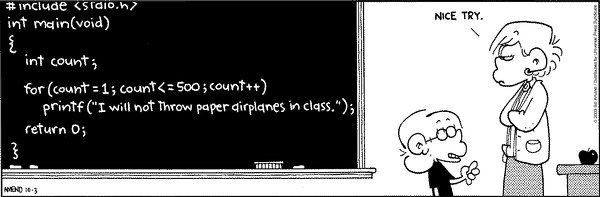
\includegraphics[width=0.95\linewidth]{images/foxtrot-loop} 

}

\caption{Foxtrot, October 3, 2003.  Used with permission.}\label{fig:flow-loop}
\end{figure}

In the above scene from the comic-strip \emph{Foxtrot}, young Jason has
tried to attempted to short-cut his ``write-on-the-blackboard''
punishment via some code in the C-language that would print out his
assigned sentence 500 times. This is an example of \emph{flow control.}
\index{flow control}

Flow control encompasses the tools in a programming language that allow
the computer to make decisions and to repeat tasks. In this Chapter we
will learn how flow control is implemented in R.

\newpage

\section{Prologue: Prompting the
User}\label{prologue-prompting-the-user}

Before we get started with flow control itself, let's address the
question of how we might extract information from someone who runs our
our code.

Up to this point any information that we have wanted to process has had
to be entered into the code itself. For example, if we want to print out
a name to the console, we have to provide that name in the code, like
this:

\begin{Shaded}
\begin{Highlighting}[]
\NormalTok{person <-}\StringTok{ "Dorothy"}
\KeywordTok{cat}\NormalTok{(}\StringTok{"Hello, "}\NormalTok{, person, }\StringTok{"!}\CharTok{\textbackslash{}n}\StringTok{"}\NormalTok{, }\DataTypeTok{sep =} \StringTok{""}\NormalTok{)}
\end{Highlighting}
\end{Shaded}

\begin{verbatim}
## Hello, Dorothy!
\end{verbatim}

We can get any printout we like as long as we assign the desired string
to \texttt{person}---but we have to do that \emph{in the code itself}.
But what if we don't know the name of the person whom we want to greet?
How can we be assured of printing out the correct name?

The \texttt{readline()}
\index{R-functions!readline()@\texttt{readline()}}function will be
helpful, here. It reads input directly from the console and produces a
character vector (of length one) that we may use as we like. Thus

\begin{Shaded}
\begin{Highlighting}[]
\NormalTok{person <-}\StringTok{ }\KeywordTok{readline}\NormalTok{(}\DataTypeTok{prompt =} \StringTok{"What is your name?  "}\NormalTok{)}
\KeywordTok{cat}\NormalTok{(}\StringTok{"Hello, "}\NormalTok{, person, }\StringTok{"!}\CharTok{\textbackslash{}n}\StringTok{"}\NormalTok{, }\DataTypeTok{sep =} \StringTok{""}\NormalTok{)}
\end{Highlighting}
\end{Shaded}

\begin{verbatim}
## What is your name?  Cowardly Lion
## Hello, Cowardly Lion!
\end{verbatim}

Note that the input obtained from \texttt{readline()} is always a
character vector of length one---a single string---so if you plan to use
it as a number then you need to convert it to a number. The
\texttt{as.numeric()}
\index{R-functions!as.numeric()@\texttt{as.numeric()}}function will do
this for you:

\begin{Shaded}
\begin{Highlighting}[]
\NormalTok{number <-}\StringTok{ }\KeywordTok{readline}\NormalTok{(}\StringTok{"Give me a number, and I'll add 10 to it:  "}\NormalTok{)}
\KeywordTok{cat}\NormalTok{(}\StringTok{"The sum is:  "}\NormalTok{, }\KeywordTok{as.numeric}\NormalTok{(number) +}\DecValTok{10}\NormalTok{)}
\end{Highlighting}
\end{Shaded}

\begin{verbatim}
## Give me a number, and I'll add 10 to it:  15
## The sum is:  25
\end{verbatim}

\section{Making Decisions:
Conditionals}\label{making-decisions-conditionals}

We are now ready to begin addressing flow control itself. We'll begin by
looking at the various facilities R has for making decisions.

\subsection{If Statements}\label{if-statements}

Let's design a simple guessing-game for the user:

\begin{itemize}
\tightlist
\item
  The computer will pick randomly a whole number between 1 and 4.
\item
  The user will then be asked to guess the number.
\item
  If the user is correct, then the computer will congratulate the user.
\end{itemize}

\begin{Shaded}
\begin{Highlighting}[]
\NormalTok{number <-}\StringTok{ }\KeywordTok{sample}\NormalTok{(}\DecValTok{1}\NormalTok{:}\DecValTok{4}\NormalTok{, }\DataTypeTok{size =} \DecValTok{1}\NormalTok{)}
\NormalTok{guess <-}\StringTok{ }\KeywordTok{as.numeric}\NormalTok{(}\KeywordTok{readline}\NormalTok{(}\StringTok{"Guess the number (1-4):  "}\NormalTok{))}
\NormalTok{if ( guess ==}\StringTok{ }\NormalTok{number ) \{}
  \KeywordTok{cat}\NormalTok{(}\StringTok{"Congratulations!  You are correct."}\NormalTok{)}
\NormalTok{\}}
\end{Highlighting}
\end{Shaded}

The \texttt{sample()}
\index{R-functions!sample()@\texttt{sample()}}function randomly picks a
value from the vector that is is given. The \texttt{size} parameter
specifies how many numbers to pick. (This time we only want one number.)

Flow control enters the picture with the reserved word
\texttt{if}\index{if@\texttt{if}}. Immediately after \texttt{if} is a
Boolean expression enclosed in parentheses. This expression is often
called the \emph{condition}. \index{condition}If the condition evaluates
to \texttt{TRUE}, then the body of the \texttt{if} statement---the code
enclosed in the brackets---will be executed. On the other hand if the
condition evaluates to \texttt{FALSE}, then R skips past the bracketed
code.\footnote{Actually you don't need the brackets if you plan to put
  only one expression in them. Many people keep the brackets, though,
  for the sake of clarity.}

The code above congratulates the a lucky guesser, but it has nothing at
all to say to someone who did not guess correctly. The way to provide an
alternative is through the addition of the \texttt{else}
reserved-word\index{if ... else@\texttt{if ... else}}:

\begin{Shaded}
\begin{Highlighting}[]
\NormalTok{number <-}\StringTok{ }\KeywordTok{sample}\NormalTok{(}\DecValTok{1}\NormalTok{:}\DecValTok{4}\NormalTok{, }\DataTypeTok{size =} \DecValTok{1}\NormalTok{)}
\NormalTok{guess <-}\StringTok{ }\KeywordTok{as.numeric}\NormalTok{(}\KeywordTok{readline}\NormalTok{(}\StringTok{"Guess the number (1-4):  "}\NormalTok{))}
\NormalTok{if ( guess ==}\StringTok{ }\NormalTok{number ) \{}
  \KeywordTok{cat}\NormalTok{(}\StringTok{"Congratulations!  You are correct."}\NormalTok{)}
\NormalTok{\} else \{}
  \KeywordTok{cat}\NormalTok{(}\StringTok{"Sorry, the correct number was "}\NormalTok{, number, }\StringTok{".}\CharTok{\textbackslash{}n}\StringTok{"}\NormalTok{, }\DataTypeTok{sep =} \StringTok{""}\NormalTok{)}
  \KeywordTok{cat}\NormalTok{(}\StringTok{"Better luck next time!"}\NormalTok{)}
\NormalTok{\}}
\end{Highlighting}
\end{Shaded}

An \texttt{if-else}can be followed by any number of \texttt{if-else}'s,
setting up a chain of alternative responses:

\begin{Shaded}
\begin{Highlighting}[]
\NormalTok{number <-}\StringTok{ }\KeywordTok{sample}\NormalTok{(}\DecValTok{1}\NormalTok{:}\DecValTok{4}\NormalTok{, }\DataTypeTok{size =} \DecValTok{1}\NormalTok{)}
\NormalTok{guess <-}\StringTok{ }\KeywordTok{as.numeric}\NormalTok{(}\KeywordTok{readline}\NormalTok{(}\StringTok{"Guess the number (1-4):  "}\NormalTok{))}
\NormalTok{if ( guess ==}\StringTok{ }\NormalTok{number ) \{}
  \KeywordTok{cat}\NormalTok{(}\StringTok{"Congratulations!  You are correct."}\NormalTok{)}
\NormalTok{\} else if ( }\KeywordTok{abs}\NormalTok{(guess -}\StringTok{ }\NormalTok{number) ==}\StringTok{ }\DecValTok{1} \NormalTok{)\{}
  \KeywordTok{cat}\NormalTok{(}\StringTok{"You were close!}\CharTok{\textbackslash{}n}\StringTok{"}\NormalTok{)}
  \KeywordTok{cat}\NormalTok{(}\StringTok{"The correct number was "}\NormalTok{, number, }\StringTok{".}\CharTok{\textbackslash{}n}\StringTok{"}\NormalTok{, }\DataTypeTok{sep =} \StringTok{""}\NormalTok{)}
\NormalTok{\} else \{}
  \KeywordTok{cat}\NormalTok{(}\StringTok{"You were way off.}\CharTok{\textbackslash{}n}\StringTok{"}\NormalTok{)}
  \KeywordTok{cat}\NormalTok{(}\StringTok{"The correct number was "}\NormalTok{, number, }\StringTok{".}\CharTok{\textbackslash{}n}\StringTok{"}\NormalTok{, }\DataTypeTok{sep =} \StringTok{""}\NormalTok{)}
\NormalTok{\}}
\end{Highlighting}
\end{Shaded}

\subsection{Application: Invisible Returns}\label{invisible-returns}

Let's think again about the \(\pi\)-computing function from Section
\ref{default-arguments}:

\begin{Shaded}
\begin{Highlighting}[]
\NormalTok{madhavaPI <-}\StringTok{ }\NormalTok{function(}\DataTypeTok{n =} \DecValTok{1000000}\NormalTok{) \{}
  \NormalTok{k <-}\StringTok{ }\DecValTok{1}\NormalTok{:n}
  \NormalTok{terms <-}\StringTok{ }\NormalTok{(-}\DecValTok{1}\NormalTok{)^(k}\DecValTok{+1}\NormalTok{)*}\DecValTok{4}\NormalTok{/(}\DecValTok{2}\NormalTok{*k}\DecValTok{-1}\NormalTok{)}
  \KeywordTok{sum}\NormalTok{(terms)}
\NormalTok{\}}
\end{Highlighting}
\end{Shaded}

We could use \texttt{if} to write in a ``talky'' option:

\begin{Shaded}
\begin{Highlighting}[]
\NormalTok{madhavaPI <-}\StringTok{ }\NormalTok{function(}\DataTypeTok{n =} \DecValTok{1000000}\NormalTok{, }\DataTypeTok{verbose =} \OtherTok{FALSE}\NormalTok{) \{}
  \NormalTok{k <-}\StringTok{ }\DecValTok{1}\NormalTok{:n}
  \NormalTok{terms <-}\StringTok{ }\NormalTok{(-}\DecValTok{1}\NormalTok{)^(k}\DecValTok{+1}\NormalTok{)*}\DecValTok{4}\NormalTok{/(}\DecValTok{2}\NormalTok{*k}\DecValTok{-1}\NormalTok{)}
  \NormalTok{approx <-}\StringTok{ }\KeywordTok{sum}\NormalTok{(terms)}
  \NormalTok{if ( verbose) \{}
    \KeywordTok{cat}\NormalTok{(}\StringTok{"Madhava's approximation is:  "}\NormalTok{, approx, }\StringTok{".}\CharTok{\textbackslash{}n}\StringTok{"}\NormalTok{, }\DataTypeTok{sep =} \StringTok{""}\NormalTok{)}
    \KeywordTok{cat}\NormalTok{(}\StringTok{"This is based on "}\NormalTok{, n, }\StringTok{" terms.}\CharTok{\textbackslash{}n}\StringTok{"}\NormalTok{, }\DataTypeTok{sep =} \StringTok{""}\NormalTok{)}
  \NormalTok{\}}
  \NormalTok{approx}
\NormalTok{\}}
\end{Highlighting}
\end{Shaded}

Try it out:

\begin{Shaded}
\begin{Highlighting}[]
\KeywordTok{madhavaPI}\NormalTok{(}\DataTypeTok{n =} \DecValTok{1000}\NormalTok{, }\DataTypeTok{verbose =} \OtherTok{TRUE}\NormalTok{)}
\end{Highlighting}
\end{Shaded}

\begin{verbatim}
## Madhava's approximation is:  3.140593.
## This is based on 1000 terms.
\end{verbatim}

\begin{verbatim}
## [1] 3.140593
\end{verbatim}

It's a bit awkward that the approximation gets printed out at the end:
after the message on the console, the user doesn't need to see it. But
if we were to remove the final \texttt{approx} expression, then the
function would not return an approximation that could be used for
further computations.

The solution to this dilemma is R's \texttt{invisible()} function.
\index{R-functions!invisible()@\texttt{invisible()}}

\begin{Shaded}
\begin{Highlighting}[]
\NormalTok{madhavaPI <-}\StringTok{ }\NormalTok{function(}\DataTypeTok{n =} \DecValTok{1000000}\NormalTok{, }\DataTypeTok{verbose =} \OtherTok{FALSE}\NormalTok{) \{}
  \NormalTok{k <-}\StringTok{ }\DecValTok{1}\NormalTok{:n}
  \NormalTok{terms <-}\StringTok{ }\NormalTok{(-}\DecValTok{1}\NormalTok{)^(k}\DecValTok{+1}\NormalTok{)*}\DecValTok{4}\NormalTok{/(}\DecValTok{2}\NormalTok{*k}\DecValTok{-1}\NormalTok{)}
  \NormalTok{approx <-}\StringTok{ }\KeywordTok{sum}\NormalTok{(terms)}
  \NormalTok{if ( verbose) \{}
    \KeywordTok{cat}\NormalTok{(}\StringTok{"Madhava's approximation is:  "}\NormalTok{, approx, }\StringTok{".}\CharTok{\textbackslash{}n}\StringTok{"}\NormalTok{, }\DataTypeTok{sep =} \StringTok{""}\NormalTok{)}
    \KeywordTok{cat}\NormalTok{(}\StringTok{"This is based on "}\NormalTok{, n, }\StringTok{" terms.}\CharTok{\textbackslash{}n}\StringTok{"}\NormalTok{, }\DataTypeTok{sep =} \StringTok{""}\NormalTok{)}
  \NormalTok{\}}
  \KeywordTok{invisible}\NormalTok{(approx)}
\NormalTok{\}}
\end{Highlighting}
\end{Shaded}

If you wrap an expression in \texttt{invisible()}, then it won't be
printed out to the console:

\begin{Shaded}
\begin{Highlighting}[]
\KeywordTok{madhavaPI}\NormalTok{(}\DataTypeTok{n =} \DecValTok{1000}\NormalTok{, }\DataTypeTok{verbose =} \OtherTok{TRUE}\NormalTok{)}
\end{Highlighting}
\end{Shaded}

\begin{verbatim}
## Madhava's approximation is:  3.140593.
## This is based on 1000 terms.
\end{verbatim}

Nevertheless it is still returned, as we can see from the following
code, in which the approximation is computed without any output to the
console and stored in the variable \texttt{p} for use later on in a
\texttt{cat()} statement.

\begin{Shaded}
\begin{Highlighting}[]
\NormalTok{p <-}\StringTok{ }\KeywordTok{madhavaPI}\NormalTok{() }\CommentTok{# verbose is FALSE by default}
\KeywordTok{cat}\NormalTok{(}\StringTok{"Pi plus 10 is about "}\NormalTok{, p +}\StringTok{ }\DecValTok{10}\NormalTok{, }\StringTok{"."}\NormalTok{, }\DataTypeTok{sep =} \StringTok{""}\NormalTok{)}
\end{Highlighting}
\end{Shaded}

\begin{verbatim}
## Pi plus 10 is about 13.14159.
\end{verbatim}

\subsection{Ifelse}\label{ifelse}

The \texttt{ifelse()}
\index{R-functions!ifelse()@\texttt{ifelse()}}function is a special form
of the if-else construct that is used to make assignments, and is
especially handy in the context of vectorization.

Suppose that you have a lot of heights:

\begin{Shaded}
\begin{Highlighting}[]
\NormalTok{height <-}\StringTok{ }\KeywordTok{c}\NormalTok{(}\DecValTok{69}\NormalTok{, }\DecValTok{67}\NormalTok{, }\DecValTok{70}\NormalTok{, }\DecValTok{72}\NormalTok{, }\DecValTok{65}\NormalTok{, }\DecValTok{63}\NormalTok{, }\DecValTok{75}\NormalTok{, }\DecValTok{70}\NormalTok{)}
\end{Highlighting}
\end{Shaded}

You would like to classify each person as either ``tall'' or ``short'',
depending on whether they are respectively more or less than 71 inches
in height. \texttt{ifelse()} makes quick work of it:

\begin{Shaded}
\begin{Highlighting}[]
\NormalTok{heightClass <-}\StringTok{ }\KeywordTok{ifelse}\NormalTok{(}\DataTypeTok{test =} \NormalTok{height >}\StringTok{ }\DecValTok{70}\NormalTok{, }
                      \DataTypeTok{yes =} \StringTok{"tall"}\NormalTok{, }\DataTypeTok{no =} \StringTok{"short"}\NormalTok{)}
\NormalTok{heightClass}
\end{Highlighting}
\end{Shaded}

\begin{verbatim}
## [1] "short" "short" "short" "tall"  "short" "short" "tall"  "short"
\end{verbatim}

Note that \texttt{ifelse()} takes three parameters:

\begin{itemize}
\tightlist
\item
  \texttt{test}: the condition you want to evaluate;
\item
  \texttt{yes}: the value that gets assigned when \texttt{test} is true;
\item
  \texttt{no}: the value assigned when \texttt{test} is false;
\end{itemize}

Most programmers don't name the parameters. This is fine---just remember
to keep the test-yes-no order:

\begin{Shaded}
\begin{Highlighting}[]
\KeywordTok{ifelse}\NormalTok{(height >}\StringTok{ }\DecValTok{70}\NormalTok{, }\StringTok{"tall"}\NormalTok{, }\StringTok{"short"}\NormalTok{)}
\end{Highlighting}
\end{Shaded}

\begin{verbatim}
## [1] "short" "short" "short" "tall"  "short" "short" "tall"  "short"
\end{verbatim}

Here's another example of the power of \texttt{ifelese()}. If a triangle
has three sides of length \(x\), \(y\) and \(z\), then the sum of any
two sides must be greater than the remaining side:

\[\begin{aligned}
x + y &> z, \\
x + z &> y, \\
y + z &> x.
\end{aligned}\] This fact is known as the \emph{Triangle Inequality}. It
works the other way around, too: if three positive numbers are such that
the sum of any two exceeds the third, then three line segments having
those numbers as lengths could be arranged into a triangle.

We can write a function that, when given three lengths, determines
whether or not they can make a triangle:

\begin{Shaded}
\begin{Highlighting}[]
\NormalTok{isTriangle <-}\StringTok{ }\NormalTok{function(x, y, z) \{}
  \NormalTok{(x +}\StringTok{ }\NormalTok{y >}\StringTok{ }\NormalTok{z) &}\StringTok{ }\NormalTok{(x +z >}\StringTok{ }\NormalTok{y) &}\StringTok{ }\NormalTok{(y +}\StringTok{ }\NormalTok{z >}\StringTok{ }\NormalTok{x)}
\NormalTok{\}}
\end{Highlighting}
\end{Shaded}

\texttt{isTriangle()} simply evaluates a Boolean expression involving
\texttt{x}, \texttt{y} and \texttt{z}. It will return \texttt{TRUE} when
the three quantities satisfy the Triangle Inequality; otherwise, it
returns \texttt{FALSE}. Let's try it out:

\begin{Shaded}
\begin{Highlighting}[]
\KeywordTok{isTriangle}\NormalTok{(}\DataTypeTok{x =} \DecValTok{3}\NormalTok{, }\DataTypeTok{y =} \DecValTok{4}\NormalTok{, }\DataTypeTok{z =} \DecValTok{5}\NormalTok{)}
\end{Highlighting}
\end{Shaded}

\begin{verbatim}
## [1] TRUE
\end{verbatim}

Recall that Boolean expressions can involve vectors of any length. So
suppose that we are would like to know which of the following six
triples of numbers could be the side-lengths of a triangle:

\[(2,4,5),(4.7,1,3.8),(5.2,8,12),\\
(6, 6, 13), (6, 6, 11), (9, 3.5, 6.2)\] We could enter the triples one
at a time into \texttt{isTriangle()}. On the other hand we could arrange
the sides into three vectors of length six each:

\begin{Shaded}
\begin{Highlighting}[]
\NormalTok{a <-}\StringTok{ }\KeywordTok{c}\NormalTok{(}\DecValTok{2}\NormalTok{, }\FloatTok{4.7}\NormalTok{, }\FloatTok{5.2}\NormalTok{, }\DecValTok{6}\NormalTok{, }\DecValTok{6}\NormalTok{, }\DecValTok{9}\NormalTok{)}
\NormalTok{b <-}\StringTok{ }\KeywordTok{c}\NormalTok{(}\DecValTok{4}\NormalTok{, }\DecValTok{1}\NormalTok{, }\FloatTok{2.8}\NormalTok{, }\DecValTok{6}\NormalTok{, }\DecValTok{6}\NormalTok{, }\FloatTok{3.5}\NormalTok{)}
\NormalTok{c <-}\StringTok{ }\KeywordTok{c}\NormalTok{(}\DecValTok{5}\NormalTok{, }\FloatTok{3.8}\NormalTok{, }\DecValTok{12}\NormalTok{, }\DecValTok{13}\NormalTok{, }\DecValTok{11}\NormalTok{, }\FloatTok{6.2}\NormalTok{)}
\end{Highlighting}
\end{Shaded}

Then we can decide about all six triples at once:

\begin{Shaded}
\begin{Highlighting}[]
\KeywordTok{isTriangle}\NormalTok{(}\DataTypeTok{x =} \NormalTok{a, }\DataTypeTok{y =} \NormalTok{b, }\DataTypeTok{z =} \NormalTok{c)}
\end{Highlighting}
\end{Shaded}

\begin{verbatim}
## [1]  TRUE  TRUE FALSE FALSE  TRUE  TRUE
\end{verbatim}

We could also use \texttt{ifelse()} to create a new character-vector
that expresses our results verbally:

\begin{Shaded}
\begin{Highlighting}[]
\NormalTok{triangle <-}\StringTok{ }\KeywordTok{ifelse}\NormalTok{(}\KeywordTok{isTriangle}\NormalTok{(a, b, c), }\StringTok{"triangle"}\NormalTok{, }\StringTok{"not"}\NormalTok{)}
\NormalTok{triangle}
\end{Highlighting}
\end{Shaded}

\begin{verbatim}
## [1] "triangle" "triangle" "not"      "not"      "triangle" "triangle"
\end{verbatim}

\subsection{Switch}\label{switch}

If you have to make a decision involving two or more alternatives you
can use a chain of \texttt{if\ ...\ else} constructions. When the
alternatives involve no more than the assignment of a value to a
variable, you might also consider using the
\texttt{switch()}\index{R-functions!switch()@\texttt{switch()}}
function.

For example, suppose that you have days of the week expressed as
numbers. Maybe it's like this:

\begin{itemize}
\tightlist
\item
  1 stands for Sunday
\item
  2 for Monday
\item
  3 for Wednesday
\item
  and so on.
\end{itemize}

If you would like to convert a day-number to the right day name, then
you could write a function like this:

\begin{Shaded}
\begin{Highlighting}[]
\NormalTok{dayWord <-}\StringTok{ }\NormalTok{function(dayNumber) \{}
  \NormalTok{switch(dayNumber,}
         \StringTok{"Sunday"}\NormalTok{,}
         \StringTok{"Monday"}\NormalTok{,}
         \StringTok{"Tuesday"}\NormalTok{,}
         \StringTok{"Wednesday"}\NormalTok{,}
         \StringTok{"Thursday"}\NormalTok{,}
         \StringTok{"Friday"}\NormalTok{,}
         \StringTok{"Saturday"}\NormalTok{)}
\NormalTok{\}}
\KeywordTok{dayWord}\NormalTok{(}\DecValTok{3}\NormalTok{)}
\end{Highlighting}
\end{Shaded}

\begin{verbatim}
## [1] "Tuesday"
\end{verbatim}

In \texttt{switch()} above, the first argument after \texttt{dayNumber}
is what goes with 1, the second argument is what goes with 2, and so on.

When the item you want to convert is a string rather than a number, then
the \texttt{switch()} function works a little bit differently. Suppose,
for instance, that you want to \emph{abbreviate} the names of the
weekdays. You might write an abbreviation-function as follows:

\begin{Shaded}
\begin{Highlighting}[]
\NormalTok{abbrDay <-}\StringTok{ }\NormalTok{function(day) \{}
  \NormalTok{switch(day,}
         \DataTypeTok{Monday =} \StringTok{"Mon"}\NormalTok{,}
         \DataTypeTok{Tuesday =} \StringTok{"Tue"}\NormalTok{,}
         \DataTypeTok{Wednesday =} \StringTok{"Wed"}\NormalTok{,}
         \DataTypeTok{Thursday =} \StringTok{"Th"}\NormalTok{,}
         \DataTypeTok{Friday =} \StringTok{"Fri"}\NormalTok{,}
         \DataTypeTok{Saturday =} \StringTok{"Sat"}\NormalTok{)}
\NormalTok{\}}
\KeywordTok{abbrDay}\NormalTok{(}\StringTok{"Wednesday"}\NormalTok{)}
\end{Highlighting}
\end{Shaded}

\begin{verbatim}
## [1] "Wed"
\end{verbatim}

In the above call to \texttt{switch()}, the weekday names you want to
abbreviate appear as the names of named character-vectors, each of
length one. The value of each vector is what the its name will be
converted to.

When you are converting strings you have the option to provide a default
conversion for values that don't fit into the pattern you have in mind.
All you have to do is to provide the default value as an additional
argument. (It should NOT have a name.) Thus:

\begin{Shaded}
\begin{Highlighting}[]
\NormalTok{abbrDay <-}\StringTok{ }\NormalTok{function(day) \{}
  \NormalTok{switch(day,}
         \DataTypeTok{Monday =} \StringTok{"Mon"}\NormalTok{,}
         \DataTypeTok{Tuesday =} \StringTok{"Tue"}\NormalTok{,}
         \DataTypeTok{Wednesday =} \StringTok{"Wed"}\NormalTok{,}
         \DataTypeTok{Thursday =} \StringTok{"Th"}\NormalTok{,}
         \DataTypeTok{Friday =} \StringTok{"Fri"}\NormalTok{,}
         \DataTypeTok{Saturday =} \StringTok{"Sat"}\NormalTok{,}
         \StringTok{"not a weekday!"}\NormalTok{)}
\NormalTok{\}}
\KeywordTok{abbrDay}\NormalTok{(}\StringTok{"Wednesday"}\NormalTok{)}
\end{Highlighting}
\end{Shaded}

\begin{verbatim}
## [1] "Wed"
\end{verbatim}

\begin{Shaded}
\begin{Highlighting}[]
\KeywordTok{abbrDay}\NormalTok{(}\StringTok{"Neptune"}\NormalTok{)}
\end{Highlighting}
\end{Shaded}

\begin{verbatim}
## [1] "not a weekday!"
\end{verbatim}

\section{Repeating Things: Looping}\label{repeating-things-looping}

We have looked a bit into the aspect of flow control that pertains to
making decisions. Let us now turn to the R-constructs that make the
computer repeat actions.

\subsection{For Loops}\label{for-loops}

\index{for}

The reserved word \texttt{for} \index{for@\texttt{for}}is used to make R
repeat an action a specified number of times.

We begin with an very simple example:

\begin{Shaded}
\begin{Highlighting}[]
\NormalTok{for ( i in }\DecValTok{1}\NormalTok{:}\DecValTok{4} \NormalTok{) \{}
  \KeywordTok{cat}\NormalTok{(}\StringTok{"Hello, Dorothy!}\CharTok{\textbackslash{}n}\StringTok{"}\NormalTok{)}
\NormalTok{\}}
\end{Highlighting}
\end{Shaded}

\begin{verbatim}
## Hello, Dorothy!
## Hello, Dorothy!
## Hello, Dorothy!
## Hello, Dorothy!
\end{verbatim}

Here's how the loop works. Recall that the vector \texttt{1:4} is simply
the sequence of integers from 1 to 4:

\begin{Shaded}
\begin{Highlighting}[]
\DecValTok{1}\NormalTok{:}\DecValTok{4}
\end{Highlighting}
\end{Shaded}

\begin{verbatim}
## [1] 1 2 3 4
\end{verbatim}

When R sees the code \texttt{(i\ in\ 1:4)} it knows that it will have to
go four times through the body of the loop.

\begin{Shaded}
\begin{Highlighting}[]
\KeywordTok{cat}\NormalTok{(}\StringTok{"Hello, Dorothy!}\CharTok{\textbackslash{}n}\StringTok{"}\NormalTok{)}
\end{Highlighting}
\end{Shaded}

(The \emph{body} of a loop is what's contained in the brackets after
\texttt{for(i\ in\ 1:4)}). At the start of the loop, the \emph{index
variable}\index{index variable} \texttt{i} is set to 1. After the body
is executed the first time, R sets \texttt{i} to 2, then executes the
body again. Then R sets \texttt{i} to 3 and executes the body yet again.
Then R sets \texttt{i} to 4, and executes the body for the final time.
The result is four lines printed out to the console.

The more you need to repeat a particular pattern, the more it makes
sense to write your code with a loop.

The general for of a loop is:

\begin{Shaded}
\begin{Highlighting}[]
\NormalTok{for ( var in seq ) \{}
  \NormalTok{expression}
  \NormalTok{another expression}
  \NormalTok{...}
  \NormalTok{final expression}
\NormalTok{\}}
\end{Highlighting}
\end{Shaded}

\texttt{var} is the index variable, and it can be any permitted name for
a variable, and \texttt{seq} can be any vector. As R traverses the loop,
the value of the index variable \texttt{var} becomes each element of the
vector \texttt{seq} in turn. With every change in the value of
\texttt{var}, the code in the brackets is executed.

To \emph{iterate} is to do a thing again and again. The vector
\texttt{seq} is sometimes called an \emph{iterable}, since it is
``iterated over.'' It contains the values that the index variable will
assume, one by one, as the loop is repeated. \index{iterable}

It's important to realize that the index variable can have \emph{any}
valid name, and the sequence can be any type of vector at all---not just
a sequence of consecutive whole numbers beginning with 1. This level of
generality permits a for-loop to automate a wide variety of tasks, and
for its code to be written in a way that evokes the operations being
performed.

For example, here is a loop to print out some greetings;

\begin{Shaded}
\begin{Highlighting}[]
\NormalTok{people <-}\StringTok{ }\KeywordTok{c}\NormalTok{(}\StringTok{"Dorothy"}\NormalTok{, }\StringTok{"Tin Man"}\NormalTok{, }\StringTok{"Scarecrow"}\NormalTok{, }\StringTok{"Lion"}\NormalTok{)}
\NormalTok{for ( person in people ) \{}
  \KeywordTok{cat}\NormalTok{(}\StringTok{"Hello, "}\NormalTok{, person, }\StringTok{"!}\CharTok{\textbackslash{}n}\StringTok{"}\NormalTok{, }\DataTypeTok{sep =} \StringTok{""}\NormalTok{)}
\NormalTok{\}}
\end{Highlighting}
\end{Shaded}

\begin{verbatim}
## Hello, Dorothy!
## Hello, Tin Man!
## Hello, Scarecrow!
## Hello, Lion!
\end{verbatim}

Or perhaps you want to abbreviate a vector-ful of weekday-names:

\begin{Shaded}
\begin{Highlighting}[]
\NormalTok{weekdays <-}\StringTok{ }\KeywordTok{c}\NormalTok{(}\StringTok{"Saturday"}\NormalTok{, }\StringTok{"Monday"}\NormalTok{, }\StringTok{"Friday"}\NormalTok{, }\StringTok{"Saturday"}\NormalTok{)}
\NormalTok{for ( day in weekdays ) \{}
  \KeywordTok{print}\NormalTok{(}\KeywordTok{abbrDay}\NormalTok{(day))}
\NormalTok{\}}
\end{Highlighting}
\end{Shaded}

\begin{verbatim}
## [1] "Sat"
## [1] "Mon"
## [1] "Fri"
## [1] "Sat"
\end{verbatim}

Quite often you will want to store the results of your trips through the
loop. Let's do this for our abbreviated weekdays:

\begin{Shaded}
\begin{Highlighting}[]
\NormalTok{weekdays <-}\StringTok{ }\KeywordTok{c}\NormalTok{(}\StringTok{"Saturday"}\NormalTok{, }\StringTok{"Monday"}\NormalTok{, }\StringTok{"Friday"}\NormalTok{, }\StringTok{"Saturday"}\NormalTok{)}
\NormalTok{abbrDays <-}\StringTok{ }\KeywordTok{character}\NormalTok{(}\KeywordTok{length}\NormalTok{(weekdays))}
\end{Highlighting}
\end{Shaded}

We used the \texttt{character()} function
\index{R-functions!character()@\texttt{character()}} to create the
character vector \texttt{abbrDays}. We specified that the number of
elements in \texttt{abbrDays} shall be the same as the number of
elements in \texttt{weekdays}. Right now \texttt{abbrDays} isn't very
interesting, as all of its elements are empty strings:

\begin{Shaded}
\begin{Highlighting}[]
\NormalTok{abbrDays}
\end{Highlighting}
\end{Shaded}

\begin{verbatim}
## [1] "" "" "" ""
\end{verbatim}

We will now write a for-loop to fill it up with abbreviations:

\begin{Shaded}
\begin{Highlighting}[]
\NormalTok{for ( i in }\DecValTok{1}\NormalTok{:}\KeywordTok{length}\NormalTok{(weekdays) ) \{}
  \NormalTok{abbrDays[i] <-}\StringTok{ }\KeywordTok{abbrDay}\NormalTok{(weekdays[i])}
\NormalTok{\}}
\end{Highlighting}
\end{Shaded}

Now each of the four elements of \texttt{abbrDays} contains the
abbreviation for the corresponding element of \texttt{weekdays}:

\begin{Shaded}
\begin{Highlighting}[]
\NormalTok{abbrDays}
\end{Highlighting}
\end{Shaded}

\begin{verbatim}
## [1] "Sat" "Mon" "Fri" "Sat"
\end{verbatim}

\subsection{For-Loop Caution}\label{for-loop-caution}

You might need to exercise some caution in your choice name for the
index variable. If you are already using it as the name for a variable
in the same environment, then you will overwrite that variable, as
demonstrated by the following code:

\begin{Shaded}
\begin{Highlighting}[]
\NormalTok{day <-}\StringTok{ "Thursday"}
\KeywordTok{cat}\NormalTok{(}\StringTok{"Today is "}\NormalTok{, day, }\StringTok{".}\CharTok{\textbackslash{}n}\StringTok{"}\NormalTok{, }\DataTypeTok{sep =} \StringTok{""}\NormalTok{)}
\end{Highlighting}
\end{Shaded}

\begin{verbatim}
## Today is Thursday.
\end{verbatim}

\begin{Shaded}
\begin{Highlighting}[]
\NormalTok{weekdays <-}\StringTok{ }\KeywordTok{c}\NormalTok{(}\StringTok{"Saturday"}\NormalTok{, }\StringTok{"Monday"}\NormalTok{, }\StringTok{"Friday"}\NormalTok{, }\StringTok{"Saturday"}\NormalTok{)}
\NormalTok{abbrDays <-}\StringTok{ }\KeywordTok{character}\NormalTok{(}\KeywordTok{length}\NormalTok{(weekdays))}
\NormalTok{for ( day in weekdays ) \{}
  \KeywordTok{print}\NormalTok{(day)}
\NormalTok{\}}
\end{Highlighting}
\end{Shaded}

\begin{verbatim}
## [1] "Saturday"
## [1] "Monday"
## [1] "Friday"
## [1] "Saturday"
\end{verbatim}

\begin{Shaded}
\begin{Highlighting}[]
\KeywordTok{cat}\NormalTok{(}\StringTok{"Today is "}\NormalTok{, day, }\StringTok{".}\CharTok{\textbackslash{}n}\StringTok{"}\NormalTok{, }\DataTypeTok{sep =} \StringTok{""}\NormalTok{)}
\end{Highlighting}
\end{Shaded}

\begin{verbatim}
## Today is Saturday.
\end{verbatim}

Of course, that won't happen if the for-loop is inside of a function and
your variable is outside of it.

\begin{Shaded}
\begin{Highlighting}[]
\NormalTok{day <-}\StringTok{ "Thursday"}
\KeywordTok{cat}\NormalTok{(}\StringTok{"Today is "}\NormalTok{, day, }\StringTok{".}\CharTok{\textbackslash{}n}\StringTok{"}\NormalTok{, }\DataTypeTok{sep =} \StringTok{""}\NormalTok{)}
\end{Highlighting}
\end{Shaded}

\begin{verbatim}
## Today is Thursday.
\end{verbatim}

\begin{Shaded}
\begin{Highlighting}[]
\NormalTok{weekdays <-}\StringTok{ }\KeywordTok{c}\NormalTok{(}\StringTok{"Saturday"}\NormalTok{, }\StringTok{"Monday"}\NormalTok{, }\StringTok{"Friday"}\NormalTok{, }\StringTok{"Saturday"}\NormalTok{)}
\NormalTok{listDays <-}\StringTok{ }\NormalTok{function(days) \{}
  \NormalTok{for ( day in days )    \{}
    \KeywordTok{print}\NormalTok{(day)}
  \NormalTok{\}}
\NormalTok{\}}
\KeywordTok{listDays}\NormalTok{(weekdays)}
\end{Highlighting}
\end{Shaded}

\begin{verbatim}
## [1] "Saturday"
## [1] "Monday"
## [1] "Friday"
## [1] "Saturday"
\end{verbatim}

\begin{Shaded}
\begin{Highlighting}[]
\KeywordTok{cat}\NormalTok{(}\StringTok{"Today is still "}\NormalTok{, day, }\StringTok{".}\CharTok{\textbackslash{}n}\StringTok{"}\NormalTok{, }\DataTypeTok{sep =} \StringTok{""}\NormalTok{)}
\end{Highlighting}
\end{Shaded}

\begin{verbatim}
## Today is still Thursday.
\end{verbatim}

\subsection{Breaking Out of a Loop}\label{breaking-out-of-a-loop}

Sometimes you finish the task at hand before you are done with the loop.
If this is a possibility for you then you may arrange to break out of
the loop with the \texttt{break}\index{break@\texttt{break}}
reserved-word.

Suppose for example that you want a function that searches through a
vector for a given element, updating the user along the way as to the
progress of the search. You can try something like this:

\begin{Shaded}
\begin{Highlighting}[]
\CommentTok{# function to find index of element in vector.}
\CommentTok{# returns -1 if elem is not in vector}
\NormalTok{verboseSearch <-}\StringTok{ }\NormalTok{function(elem, vec) \{}
  
  \CommentTok{# The following logical keeps track of whether}
  \CommentTok{# we have found the element.}
  \CommentTok{# We have not yet begun the search so start it}
  \CommentTok{# at FALSE.}
  \NormalTok{found <-}\StringTok{ }\OtherTok{FALSE}
  
  \CommentTok{# validate input:}
  \NormalTok{if ( }\KeywordTok{length}\NormalTok{(vec) ==}\StringTok{ }\DecValTok{0} \NormalTok{) \{}
    \KeywordTok{cat}\NormalTok{(}\StringTok{"The vector empty.  No way does it contain "}\NormalTok{, }
        \NormalTok{elem, }\StringTok{"."}\NormalTok{, }\DataTypeTok{sep =} \StringTok{""}\NormalTok{)}
    \KeywordTok{return}\NormalTok{(-}\DecValTok{1}\NormalTok{)}
  \NormalTok{\}}
  
  \CommentTok{# check the elements of vector:}
  \NormalTok{for ( i in }\DecValTok{1}\NormalTok{:}\StringTok{ }\KeywordTok{length}\NormalTok{(vec) ) \{}
    \NormalTok{if ( vec[i] ==}\StringTok{ }\NormalTok{elem ) \{}
      \CommentTok{# record that we found the element:}
      \NormalTok{found <-}\StringTok{ }\OtherTok{TRUE}
      \NormalTok{break}
    \NormalTok{\} else \{}
      \CommentTok{# report no match at this index:}
      \KeywordTok{cat}\NormalTok{(}\StringTok{"Checked index "}\NormalTok{, i, }
          \StringTok{" in the vector.  No match there ...}\CharTok{\textbackslash{}n}\StringTok{"}\NormalTok{, }\DataTypeTok{sep =} \StringTok{""}\NormalTok{)}
    \NormalTok{\}}
  \NormalTok{\}}
  
  \NormalTok{if ( found ) \{}
    \CommentTok{# report success:}
    \KeywordTok{cat}\NormalTok{(}\StringTok{"Found "}\NormalTok{, elem, }\StringTok{" at index "}\NormalTok{, i, }\StringTok{".}\CharTok{\textbackslash{}n}\StringTok{"}\NormalTok{, }\DataTypeTok{sep =} \StringTok{""}\NormalTok{)}
    \KeywordTok{return}\NormalTok{(i)}
  \NormalTok{\} else \{}
    \CommentTok{# report failure:}
    \KeywordTok{cat}\NormalTok{(elem, }\StringTok{" is not in the vector.}\CharTok{\textbackslash{}n}\StringTok{"}\NormalTok{, }\DataTypeTok{sep =} \StringTok{""}\NormalTok{)}
    \KeywordTok{return}\NormalTok{(-}\DecValTok{1}\NormalTok{)}
  \NormalTok{\}}
\NormalTok{\}}
\end{Highlighting}
\end{Shaded}

Let's see our function in action:

\begin{Shaded}
\begin{Highlighting}[]
\NormalTok{people <-}\StringTok{ }\KeywordTok{c}\NormalTok{(}\StringTok{"Dorothy"}\NormalTok{, }\StringTok{"Tin Man"}\NormalTok{, }\StringTok{"Scarecrow"}\NormalTok{, }\StringTok{"Lion"}\NormalTok{)}
\NormalTok{scarecrowPlace <-}\StringTok{ }\KeywordTok{verboseSearch}\NormalTok{(}\StringTok{"Scarecrow"}\NormalTok{, people)}
\end{Highlighting}
\end{Shaded}

\begin{verbatim}
## Checked index 1 in the vector.  No match there ...
## Checked index 2 in the vector.  No match there ...
## Found Scarecrow at index 3.
\end{verbatim}

In the code for \texttt{verboseSearch()} you will notice that there is
an initial check on the length of the vector. This is actually
important. If a user were to enter an empty vector, then it length would
be 0. Then in the loop the sequence would be \texttt{1:0}, which is the
vector with elements 1 and 0. But look at what happens when you ask for
any element of a zero-length vector:

\begin{Shaded}
\begin{Highlighting}[]
\NormalTok{emptyVec <-}\StringTok{ }\KeywordTok{character}\NormalTok{(}\DecValTok{0}\NormalTok{)}
\NormalTok{emptyVec[}\DecValTok{1}\NormalTok{]  }\CommentTok{# You get NA}
\end{Highlighting}
\end{Shaded}

\begin{verbatim}
## [1] NA
\end{verbatim}

Then check out what happens if you compare an \texttt{NA} to a string:

\begin{Shaded}
\begin{Highlighting}[]
\OtherTok{NA} \NormalTok{==}\StringTok{ "Scarecrow"}
\end{Highlighting}
\end{Shaded}

\begin{verbatim}
## [1] NA
\end{verbatim}

Now look at what happens in an \texttt{if} statement where the condition
is \texttt{NA}:

\begin{Shaded}
\begin{Highlighting}[]
\NormalTok{if ( }\OtherTok{NA} \NormalTok{) \{}
  \KeywordTok{cat}\NormalTok{(}\StringTok{"We are in the bracket!}\CharTok{\textbackslash{}n}\StringTok{"}\NormalTok{)}
\NormalTok{\}}
\end{Highlighting}
\end{Shaded}

\begin{verbatim}
## Error in if (NA) { : missing value where TRUE/FALSE needed
\end{verbatim}

Checking that the input vector has positive length is an example of
\emph{validating} \index{validation} input. When you write functions for
other people to use you will find that it's important to validate their
input instead of allowing R to throw obscure error messages at them.

\subsection{\texorpdfstring{Solving the Empty-Vector Problem in
\texttt{for}-Loops with
\texttt{seq\_along()}}{Solving the Empty-Vector Problem in for-Loops with seq\_along()}}\label{solving-the-empty-vector-problem-in-for-loops-with-seq_along}

In the previous section we considered a possible problem with
\texttt{for}-loops of the following form:

\begin{Shaded}
\begin{Highlighting}[]
\NormalTok{for ( i in }\DecValTok{1}\NormalTok{:}\KeywordTok{length}\NormalTok{(vec) ) \{}
  \NormalTok{## do something ...}
\NormalTok{\}}
\end{Highlighting}
\end{Shaded}

In the above loop \texttt{vec} could be thought of as a
``loop-defining'' vector: its length determines the sequence of values
1, 2, 3 \ldots{} for the index \texttt{i}. This sequence of values is
supposed to end at the length of \texttt{vec}.

The problem is that if \texttt{vec} happens to be an empty vector then
we probably don't want to enter the loop at all. However, the length of
an empty vector is 0, and so the vector \texttt{1:length(vec)} actually
works out to be a vector with two elements:

\begin{Shaded}
\begin{Highlighting}[]
\KeywordTok{c}\NormalTok{(}\DecValTok{1}\NormalTok{,}\DecValTok{0}\NormalTok{)}
\end{Highlighting}
\end{Shaded}

Hence R will go through the loop twice: once when \texttt{i} is 1, and
again when \texttt{i} is 0. Depending on what the loop does, very
unexpected results could be produced.

In the previous section we dealt with the problem by writing an
\texttt{if}-statement that provides the proper response when
\texttt{vec} is empty. In many circumstances however, all we need to do
is to make sure that the loop is skipped when the vector is empty.

A handy way to ensure skipping is to use the function
\texttt{seq\_along()}
\index{R-functions!seq_along()@\texttt{seq\_along()}}. Given any
non-empty vector, \texttt{seq\_along()} produces a sequence-vector that
begins with 1 and ends with the length of the vector, thus:

\begin{Shaded}
\begin{Highlighting}[]
\NormalTok{vec <-}\StringTok{ }\KeywordTok{c}\NormalTok{(}\StringTok{"a"}\NormalTok{, }\StringTok{"d"}\NormalTok{, }\StringTok{"f"}\NormalTok{)}
\KeywordTok{seq_along}\NormalTok{(vec)}
\end{Highlighting}
\end{Shaded}

\begin{verbatim}
## [1] 1 2 3
\end{verbatim}

On the other hand, if the vector is empty, then \texttt{seq\_long()}
returns an empty numeric vector:

\begin{Shaded}
\begin{Highlighting}[]
\NormalTok{vec <-}\StringTok{ }\KeywordTok{character}\NormalTok{()}
\KeywordTok{seq_along}\NormalTok{(vec)}
\end{Highlighting}
\end{Shaded}

\begin{verbatim}
## integer(0)
\end{verbatim}

Now consider the loop inside the following function:

\begin{Shaded}
\begin{Highlighting}[]
\NormalTok{loopy <-}\StringTok{ }\NormalTok{function(vec) \{}
  \NormalTok{for ( i in }\KeywordTok{seq_along}\NormalTok{(vec) ) \{}
    \KeywordTok{cat}\NormalTok{(}\StringTok{"This time i is "}\NormalTok{, i, }\StringTok{".}\CharTok{\textbackslash{}n}\StringTok{"}\NormalTok{, }\DataTypeTok{sep =} \StringTok{""}\NormalTok{)}
  \NormalTok{\}}
\NormalTok{\}}
\end{Highlighting}
\end{Shaded}

Given a non-empty vector, it goes through the loop a number of times
equal to the length of the vector:

\begin{Shaded}
\begin{Highlighting}[]
\KeywordTok{loopy}\NormalTok{(}\KeywordTok{c}\NormalTok{(}\StringTok{"a"}\NormalTok{, }\StringTok{"d"}\NormalTok{, }\StringTok{"f"}\NormalTok{))}
\end{Highlighting}
\end{Shaded}

\begin{verbatim}
## This time i is 1.
## This time i is 2.
## This time i is 3.
\end{verbatim}

On the other hand, when given an empty vector the function does not
enter the loop at all:

\begin{Shaded}
\begin{Highlighting}[]
\KeywordTok{loopy}\NormalTok{(}\KeywordTok{character}\NormalTok{())  }\CommentTok{# no output to console!}
\end{Highlighting}
\end{Shaded}

When you are writing a program that is complex enough that you don't
know whether the loop-defining vector might be empty, it is good
practice to use \texttt{seq\_along()} as a safeguard.

\subsection{Skipping Ahead in a Loop}\label{skipping-ahead-in-a-loop}

Depending on what happens within a loop, you might sometimes wish to
skip the remaining code within the loop and proceed to the next
iteration. R provides the reserved-word \texttt{next}
\index{next@\texttt{next}} for this purpose. Here is a simple example:

\begin{Shaded}
\begin{Highlighting}[]
\NormalTok{vec <-}\StringTok{ }\KeywordTok{c}\NormalTok{(}\StringTok{"a"}\NormalTok{,}\StringTok{"e"}\NormalTok{, }\StringTok{"e"}\NormalTok{, }\StringTok{"i"}\NormalTok{, }\StringTok{"o"}\NormalTok{, }\StringTok{"u"}\NormalTok{, }\StringTok{"e"}\NormalTok{, }\StringTok{"z"}\NormalTok{)}
\CommentTok{# shout ahoy when you see the specified element}
\NormalTok{verboseAhoy <-}\StringTok{ }\NormalTok{function(elem, vec) \{}
  \NormalTok{if (}\KeywordTok{length}\NormalTok{(vec) >}\StringTok{ }\DecValTok{0}\NormalTok{) \{}
    \NormalTok{for ( i in }\DecValTok{1}\NormalTok{:}\StringTok{ }\KeywordTok{length}\NormalTok{(vec) ) \{}
      \NormalTok{if ( vec[i] !=}\StringTok{ }\NormalTok{elem) next}
      \KeywordTok{cat}\NormalTok{(}\StringTok{"Ahoy! "}\NormalTok{, elem, }\StringTok{" at index "}\NormalTok{, i, }\StringTok{"!}\CharTok{\textbackslash{}n}\StringTok{"}\NormalTok{, }\DataTypeTok{sep =} \StringTok{""}\NormalTok{)}
    \NormalTok{\}}
  \NormalTok{\}}
  
\NormalTok{\}}
\KeywordTok{verboseAhoy}\NormalTok{(}\StringTok{"e"}\NormalTok{, vec)}
\end{Highlighting}
\end{Shaded}

\begin{verbatim}
## Ahoy! e at index 2!
## Ahoy! e at index 3!
## Ahoy! e at index 7!
\end{verbatim}

When the \texttt{vec{[}i{]}\ ==\ elem} condition is true, R immediately
skips the rest of the loop, increments the value of the index variable
\texttt{i}, and runs through the loop again.

You can always accomplish the skipping without using \texttt{next}
explicitly, but it's nice to have on hand.

\subsection{Repeat}\label{repeat}

For-loops are pretty wonderful, but they are best used in circumstances
when you know how many times you will need to loop. When you need to
repeat a block of code until a certain condition occurs, then the
\texttt{repeat} \index{repeat@\texttt{repeat}}reserved-word might be a
good choice.

For example, suppose you want to play the number-guessing game with the
user, but let her keep guessing until either she gives up or gets the
correct answer. Here's an implementation using \texttt{repeat}:

\begin{Shaded}
\begin{Highlighting}[]
\NormalTok{n <-}\StringTok{ }\DecValTok{20}
\NormalTok{number <-}\StringTok{ }\KeywordTok{sample}\NormalTok{(}\DecValTok{1}\NormalTok{:n, }\DataTypeTok{size =} \DecValTok{1}\NormalTok{)}
\KeywordTok{cat}\NormalTok{(}\StringTok{"I'm thinking of a whole number from 1 to "}\NormalTok{, n, }\StringTok{".}\CharTok{\textbackslash{}n}\StringTok{"}\NormalTok{, }\DataTypeTok{sep =} \StringTok{""}\NormalTok{)}
\NormalTok{repeat \{}
  \NormalTok{guess <-}\StringTok{ }\KeywordTok{readline}\NormalTok{(}\StringTok{"What's your guess? (Enter q to quit.)  "}\NormalTok{)}
  \NormalTok{if ( guess ==}\StringTok{ "q"}  \NormalTok{) \{}
    \KeywordTok{cat}\NormalTok{(}\StringTok{"Bye!}\CharTok{\textbackslash{}n}\StringTok{"}\NormalTok{)}
    \NormalTok{break}
  \NormalTok{\} else if ( guess ==}\StringTok{ }\NormalTok{number ) \{}
    \KeywordTok{cat}\NormalTok{(}\StringTok{"You are correct!  Thanks for playing!"}\NormalTok{)}
    \NormalTok{break}
  \NormalTok{\}}
  \CommentTok{# If we get here, the guess was not correct:}
  \CommentTok{# loop will repeat!}
\NormalTok{\}}
\end{Highlighting}
\end{Shaded}

The game works well enough, but if you give it a try, you are sure to
find it a bit fatiguing. It wold be nice to give the user a hint after
an incorrect guess. Let's revise the game to tell the reader whether her
guess was high or low. While we are at it, let's cast the game into the
form of a function.

\begin{Shaded}
\begin{Highlighting}[]
\NormalTok{numberGuess <-}\StringTok{ }\NormalTok{function(n) \{}
  \NormalTok{number <-}\StringTok{ }\KeywordTok{sample}\NormalTok{(}\DecValTok{1}\NormalTok{:n, }\DataTypeTok{size =} \DecValTok{1}\NormalTok{)}
  \KeywordTok{cat}\NormalTok{(}\StringTok{"I'm thinking of a whole number from 1 to "}\NormalTok{, n, }\StringTok{".}\CharTok{\textbackslash{}n}\StringTok{"}\NormalTok{, }\DataTypeTok{sep =} \StringTok{""}\NormalTok{)}
  \NormalTok{repeat \{}
    \NormalTok{guess <-}\StringTok{ }\KeywordTok{readline}\NormalTok{(}\StringTok{"What's your guess? (Enter q to quit.)  "}\NormalTok{)}
    \NormalTok{if (guess ==}\StringTok{ "q"}\NormalTok{) \{}
      \KeywordTok{cat}\NormalTok{(}\StringTok{"Bye!}\CharTok{\textbackslash{}n}\StringTok{"}\NormalTok{)}
      \NormalTok{break}
    \NormalTok{\} else if (guess ==}\StringTok{ }\NormalTok{number) \{}
      \KeywordTok{cat}\NormalTok{(}\StringTok{"You are correct!  Thanks for playing!"}\NormalTok{)}
      \NormalTok{break}
    \NormalTok{\}}
    \CommentTok{# If we get to this point the guess was not correct.}
    \CommentTok{# Issue hint:}
    \NormalTok{hint <-}\StringTok{ }\KeywordTok{ifelse}\NormalTok{(guess >}\StringTok{ }\NormalTok{number, }\StringTok{"high"}\NormalTok{, }\StringTok{"low"}\NormalTok{)}
    \KeywordTok{cat}\NormalTok{(}\StringTok{"Your guess was "}\NormalTok{, hint, }\StringTok{".  Keep at it!}\CharTok{\textbackslash{}n}\StringTok{"}\NormalTok{, }\DataTypeTok{sep =} \StringTok{""}\NormalTok{)}
    \CommentTok{# Repeat loop}
  \NormalTok{\}}
\NormalTok{\}}
\end{Highlighting}
\end{Shaded}

A typical game:

\begin{verbatim}
> numberGuess(100)
I'm thinking of a whole number from 1 to 100.
What's your guess? (Enter q to quit.)  50
Your guess was high.  Keep at it!
What's your guess? (Enter q to quit.)  25
Your guess was high.  Keep at it!
What's your guess? (Enter q to quit.)  12
Your guess was low.  Keep at it!
What's your guess? (Enter q to quit.)  18
Your guess was low.  Keep at it!
What's your guess? (Enter q to quit.)  22
Your guess was high.  Keep at it!
What's your guess? (Enter q to quit.)  20
You are correct!  Thanks for playing!
\end{verbatim}

\subsection{While}\label{while}

The reserved word \texttt{while} \index{while@\texttt{while}}constructs
a loop that runs as long as a specified condition is true. Unlike
\texttt{repeat}, which launches directly into the loop, the condition
for \texttt{while} is evaluated prior to the body of the loop. If the
condition is false at the beginning, the code in the body of the loop is
never executed.

\texttt{verboseSearch()} could be re-written with \texttt{while}:

\begin{Shaded}
\begin{Highlighting}[]
\NormalTok{verboseSearch <-}\StringTok{ }\NormalTok{function(elem, vec) \{}
  \NormalTok{found <-}\StringTok{ }\OtherTok{FALSE}
  \NormalTok{if ( }\KeywordTok{length}\NormalTok{(vec) ==}\StringTok{ }\DecValTok{0} \NormalTok{) \{}
    \KeywordTok{cat}\NormalTok{(}\StringTok{"The vector empty.  No way does it contain "}\NormalTok{, }
        \NormalTok{elem, }\StringTok{"."}\NormalTok{, }\DataTypeTok{sep =} \StringTok{""}\NormalTok{)}
    \KeywordTok{return}\NormalTok{(-}\DecValTok{1}\NormalTok{)}
  \NormalTok{\}}
  \CommentTok{# index of vec (start looking at 1):}
  \NormalTok{i <-}\StringTok{ }\DecValTok{1}
  \NormalTok{while ( !found &}\StringTok{ }\NormalTok{i <=}\StringTok{ }\KeywordTok{length}\NormalTok{(vec) ) \{}
    \NormalTok{if ( vec[i] ==}\StringTok{ }\NormalTok{elem ) \{}
      \NormalTok{found <-}\StringTok{ }\OtherTok{TRUE}
      \NormalTok{break}
    \NormalTok{\}}
    \KeywordTok{cat}\NormalTok{(}\StringTok{"No match at position "}\NormalTok{, i, }\StringTok{" ...}\CharTok{\textbackslash{}n}\StringTok{"}\NormalTok{)}
    \NormalTok{i <-}\StringTok{ }\NormalTok{i +}\StringTok{ }\DecValTok{1}
  \NormalTok{\}}

  \NormalTok{if ( found ) \{}
    \CommentTok{# report success:}
    \KeywordTok{cat}\NormalTok{(}\StringTok{"Found "}\NormalTok{, elem, }\StringTok{" at index "}\NormalTok{, i, }\StringTok{".}\CharTok{\textbackslash{}n}\StringTok{"}\NormalTok{, }\DataTypeTok{sep =} \StringTok{""}\NormalTok{)}
    \KeywordTok{return}\NormalTok{(i)}
  \NormalTok{\} else \{}
    \CommentTok{# report failure:}
    \KeywordTok{cat}\NormalTok{(elem, }\StringTok{" is not in the vector.}\CharTok{\textbackslash{}n}\StringTok{"}\NormalTok{, }\DataTypeTok{sep =} \StringTok{""}\NormalTok{)}
    \KeywordTok{return}\NormalTok{(-}\DecValTok{1}\NormalTok{)}
  \NormalTok{\}}
\NormalTok{\}}
\end{Highlighting}
\end{Shaded}

\section{Application: The Collatz Conjecture}\label{collatz-conjecture}

Take any positive integer greater than 1. Apply the following rule,
which we will call the Collatz Rule:

\begin{itemize}
\tightlist
\item
  If the integer is even, divide it by 2;
\item
  if the integer is odd, multiply it by 3 and add 1.
\end{itemize}

Now apply the rule to the resulting number, then apply the rule again to
the number you get from that, and so on.

For example, start with 13. We proceed as follows:

\begin{itemize}
\tightlist
\item
  13 is odd, so compute \(3 \times 13 + 1 = 40\).
\item
  40 is even, so compute \(40/2 = 20\).
\item
  20 is even, so compute \(20/2 = 10\).
\item
  10 is even, so compute \(10/2 = 5\).
\item
  5 is odd, so compute \(3 \times 5+ 1 = 16\)
\item
  16 is even, so compute \(16/2 = 8\).
\item
  8 is even, so compute \(8/2 = 4\).
\item
  4 is even, so compute \(4/2 = 2\).
\item
  2 is even, so compute \(2/2 = 1\).
\item
  1 is odd, so compute \(3 \times 1 + 1 = 4\).
\item
  4 is even, so compute \(4/2 = 2\).
\item
  2 is even, so compute \(2/2 = 1\).
\end{itemize}

If we keep going, then we will cycle forever:

\[4, 2, 1, 4, 2, 1, \ldots\] In mathematics the \emph{Collatz
Conjecture} is the conjecture that for \emph{any} initial positive
number, every Collatz Sequence (the sequence formed by repeated
application of the Collatz Rule) eventually contains a 1, after which it
must cycle forever. No matter how large a number we begin with, we have
always found that it returns to 1, but mathematicians do not know if
this will be so for \emph{any} initial number.

A sequence of Collatz numbers can bounce around quite remarkably before
descending to 1. Our goal in this section is to write a function called
\texttt{collatz()} that will compute the Collatz sequence for any given
initial number and draw a graph of the sequence as well.

First, let's make a function just for the Collatz Rule itself:

\begin{Shaded}
\begin{Highlighting}[]
\NormalTok{collatzRule <-}\StringTok{ }\NormalTok{function(m) \{}
  \NormalTok{if ( m %%}\StringTok{ }\DecValTok{2} \NormalTok{==}\StringTok{ }\DecValTok{0}\NormalTok{) \{}
    \KeywordTok{return}\NormalTok{(m/}\DecValTok{2}\NormalTok{)}
  \NormalTok{\} else \{}
    \KeywordTok{return}\NormalTok{(}\DecValTok{3}\NormalTok{*m +}\StringTok{ }\DecValTok{1}\NormalTok{)}
  \NormalTok{\}}
\NormalTok{\}}
\end{Highlighting}
\end{Shaded}

(Recall that \texttt{m\ \%\%\ 2} is the remainder of \texttt{m} after it
is divided by 2. If this is 0, then \texttt{m} is even.)

Next let's try to get a function going that will print out Collatz
numbers:

\begin{Shaded}
\begin{Highlighting}[]
\NormalTok{collatz <-}\StringTok{ }\NormalTok{function(n) \{}
  \CommentTok{# n is the initial number}
  \NormalTok{while ( n >}\StringTok{ }\DecValTok{1} \NormalTok{) \{}
    \KeywordTok{cat}\NormalTok{(n, }\StringTok{" "}\NormalTok{, }\DataTypeTok{sep =} \StringTok{""}\NormalTok{)}
    \CommentTok{# get the next number and call it n:}
    \NormalTok{n <-}\StringTok{ }\KeywordTok{collatzRule}\NormalTok{(n)}
  \NormalTok{\}}
\NormalTok{\}}
\end{Highlighting}
\end{Shaded}

Let's try it out:

\begin{Shaded}
\begin{Highlighting}[]
\KeywordTok{collatz}\NormalTok{(}\DecValTok{13}\NormalTok{)}
\end{Highlighting}
\end{Shaded}

\begin{verbatim}
## 13 40 20 10 5 16 8 4 2
\end{verbatim}

So far, so good, but if we are going to graph the numbers, then we
should store them in a vector. The problem is that we don't know how
long the vector needs to be.

One possible solution is to add to the vector as we go, like this:

\begin{Shaded}
\begin{Highlighting}[]
\NormalTok{collatz <-}\StringTok{ }\NormalTok{function(n) \{}
  \NormalTok{numbers <-}\StringTok{ }\KeywordTok{numeric}\NormalTok{()}
  \NormalTok{while ( n >}\StringTok{ }\DecValTok{1} \NormalTok{) \{}
    \CommentTok{# stick n onto the end of numbers:}
    \NormalTok{numbers <-}\StringTok{ }\KeywordTok{c}\NormalTok{(numbers, n)}
    \NormalTok{n <-}\StringTok{ }\KeywordTok{collatzRule}\NormalTok{(n)}
  \NormalTok{\}}
  \KeywordTok{print}\NormalTok{(numbers)}
\NormalTok{\}}
\end{Highlighting}
\end{Shaded}

Try it out:

\begin{Shaded}
\begin{Highlighting}[]
\KeywordTok{collatz}\NormalTok{(}\DecValTok{13}\NormalTok{)}
\end{Highlighting}
\end{Shaded}

\begin{verbatim}
## [1] 13 40 20 10  5 16  8  4  2
\end{verbatim}

This looks good. There are two problems, though, if the Collatz sequence
happens to go on for a very long time.

\begin{itemize}
\item
  \textbf{Computation Time}: the user doesn't know when the sequence
  will end---if ever!---so she won't know whether a delay in production
  of the output is due to a long sequence or a problem with the program
  itself. as the sequence gets longer, the computation-time is made even
  longer by the way the following line of code works:

\begin{verbatim}
numbers <- c(numbers, n)
\end{verbatim}

  R cannot actually ``stick'' a new element onto the end of a vector.
  What it actually does is to move to a new place in memory and create
  an entirely new vector consisting of all the elements of
  \texttt{numbers} followed by the number \texttt{n}. R then assigns the
  name \texttt{numbers} to this value, freeing up the old place in
  memory where the previous \texttt{numbers} vector lived, but when a
  vector is very long copying can take a long time.
\item
  \textbf{Memory Problems} Once the \texttt{numbers} vector gets long
  enough it will use all of the memory in the computer that is available
  to R. R will crash.
\end{itemize}

In order to get around this problem, we should impose a limit on the
number of Collatz numbers that we will compute. We'll set the limit at
10,000. The user can change the limit, but should exercise caution in
doing so. Also, we'll initialize our \texttt{numbers} vector to have a
length set to this limit. We can then assign values to elements of an
\emph{already existing} vector: this is much faster than copying entire
vectors from scratch.

\begin{Shaded}
\begin{Highlighting}[]
\NormalTok{collatz <-}\StringTok{ }\NormalTok{function(n, }\DataTypeTok{limit =} \DecValTok{10000}\NormalTok{) \{}
  \CommentTok{# collatz number swill go in this vector}
  \NormalTok{numbers <-}\StringTok{ }\KeywordTok{numeric}\NormalTok{(limit)}
  \CommentTok{# keep count of how many numbers we have made:}
  \NormalTok{counter <-}\StringTok{ }\DecValTok{0}
  \NormalTok{while ( n >}\StringTok{ }\DecValTok{1} \NormalTok{&}\StringTok{ }\NormalTok{counter <}\StringTok{ }\NormalTok{limit) \{}
    \CommentTok{# need to make a new number}
    \NormalTok{counter <-}\StringTok{ }\NormalTok{counter +}\StringTok{ }\DecValTok{1}
    \CommentTok{# put the current number into the vector}
    \NormalTok{numbers[counter] <-}\StringTok{ }\NormalTok{n}
    \CommentTok{# make next Collatz number}
    \NormalTok{n <-}\StringTok{ }\KeywordTok{collatzRule}\NormalTok{(n)}
  \NormalTok{\}}
  \CommentTok{# find how many Collatz numbers we made:}
  \NormalTok{howMany <-}\StringTok{ }\KeywordTok{min}\NormalTok{(counter, limit)}
  \CommentTok{# print them out:}
  \KeywordTok{print}\NormalTok{(numbers[}\DecValTok{1}\NormalTok{:howMany])}
\NormalTok{\}}
\end{Highlighting}
\end{Shaded}

Again let's try it:

\begin{Shaded}
\begin{Highlighting}[]
\KeywordTok{collatz}\NormalTok{(}\DecValTok{257}\NormalTok{)}
\end{Highlighting}
\end{Shaded}

\begin{verbatim}
##   [1]  257  772  386  193  580  290  145  436  218  109  328  164   82   41
##  [15]  124   62   31   94   47  142   71  214  107  322  161  484  242  121
##  [29]  364  182   91  274  137  412  206  103  310  155  466  233  700  350
##  [43]  175  526  263  790  395 1186  593 1780  890  445 1336  668  334  167
##  [57]  502  251  754  377 1132  566  283  850  425 1276  638  319  958  479
##  [71] 1438  719 2158 1079 3238 1619 4858 2429 7288 3644 1822  911 2734 1367
##  [85] 4102 2051 6154 3077 9232 4616 2308 1154  577 1732  866  433 1300  650
##  [99]  325  976  488  244  122   61  184   92   46   23   70   35  106   53
## [113]  160   80   40   20   10    5   16    8    4    2
\end{verbatim}

Things are working pretty well, but since the sequence of numbers might
get pretty long, perhaps we should only print out the length of the
sequence, and leave it to the reader to say whether the sequence itself
should be shown.

\begin{Shaded}
\begin{Highlighting}[]
\NormalTok{collatz <-}\StringTok{ }\NormalTok{function(n, }\DataTypeTok{limit =} \DecValTok{10000}\NormalTok{) \{}
  \NormalTok{numbers <-}\StringTok{ }\KeywordTok{numeric}\NormalTok{(limit)}
  \NormalTok{counter <-}\StringTok{ }\DecValTok{0}
  \NormalTok{while ( n >}\StringTok{ }\DecValTok{1} \NormalTok{&}\StringTok{ }\NormalTok{counter <}\StringTok{ }\NormalTok{limit) \{}
    \NormalTok{counter <-}\StringTok{ }\NormalTok{counter +}\StringTok{ }\DecValTok{1}
    \NormalTok{numbers[counter] <-}\StringTok{ }\NormalTok{n}
    \NormalTok{n <-}\StringTok{ }\KeywordTok{collatzRule}\NormalTok{(n)}
  \NormalTok{\}}
  \NormalTok{howMany <-}\StringTok{ }\KeywordTok{min}\NormalTok{(counter, limit)}
  \KeywordTok{cat}\NormalTok{(}\StringTok{"The Collatz sequence has "}\NormalTok{, howMany, }\StringTok{" elements.}\CharTok{\textbackslash{}n}\StringTok{"}\NormalTok{, }\DataTypeTok{sep =} \StringTok{""}\NormalTok{)}
  \NormalTok{show <-}\StringTok{ }\KeywordTok{readline}\NormalTok{(}\StringTok{"Do you want to see it (y/n)?  "}\NormalTok{)}
  \NormalTok{if ( show ==}\StringTok{ "y"} \NormalTok{) \{}
    \KeywordTok{print}\NormalTok{(numbers[}\DecValTok{1}\NormalTok{:howMany])}
  \NormalTok{\}}
\NormalTok{\}}
\end{Highlighting}
\end{Shaded}

Next let's think about the plot. We'll use the plotting system in the
\textbf{ggplot2} package \citep{R-ggplot2}.

\begin{Shaded}
\begin{Highlighting}[]
\KeywordTok{library}\NormalTok{(ggplot2)}
\end{Highlighting}
\end{Shaded}

Later on we will make a serious study of plotting with \textbf{ggplot2},
but for now let's just get the basic idea of plotting a set of points.
First, let's get a small set of points to plot:

\begin{Shaded}
\begin{Highlighting}[]
\NormalTok{xvals <-}\StringTok{ }\KeywordTok{c}\NormalTok{(}\DecValTok{1}\NormalTok{, }\DecValTok{2}\NormalTok{, }\DecValTok{3}\NormalTok{, }\DecValTok{4}\NormalTok{, }\DecValTok{5}\NormalTok{)}
\NormalTok{yvals <-}\StringTok{ }\KeywordTok{c}\NormalTok{(}\DecValTok{3}\NormalTok{, }\DecValTok{7}\NormalTok{, }\DecValTok{2}\NormalTok{, }\DecValTok{4}\NormalTok{, }\DecValTok{3}\NormalTok{)}
\end{Highlighting}
\end{Shaded}

\texttt{xvals} contains the x-coordinates of our points, and
\texttt{yvals} contains the corresponding y-coordinates.

We set up a plot as follows:

\begin{Shaded}
\begin{Highlighting}[]
\NormalTok{p <-}\StringTok{ }\KeywordTok{ggplot}\NormalTok{(}\DataTypeTok{mapping =} \KeywordTok{aes}\NormalTok{(}\DataTypeTok{x =} \NormalTok{xvals, }\DataTypeTok{y =} \NormalTok{yvals))}
\end{Highlighting}
\end{Shaded}

The \texttt{ggplot()}\index{R-functions!ggplot()@\texttt{ggplot()}}
function sets up a basic two-dimensional grid. The \texttt{mapping}
parameter explains how data will be ``mapped'' to particular positions
on the plot. In this case it has been set to:

\begin{verbatim}
aes(x = xvals, y = yvals)
\end{verbatim}

\texttt{aes} is short for ``aesthetics'', which has to do with how
somethings \emph{looks}. The expression means that \texttt{xvals} will
be located on the x-axis and \texttt{yvals} will be located on the
y-axis of the plot.

Note that the entire plot has been assigned to the variable \texttt{p}.
If we want to see the plot we could print p out (see Figure
\ref{fig:blank-ggplot}):

\begin{Shaded}
\begin{Highlighting}[]
\KeywordTok{print}\NormalTok{(p)}
\end{Highlighting}
\end{Shaded}

\begin{figure}

{\centering 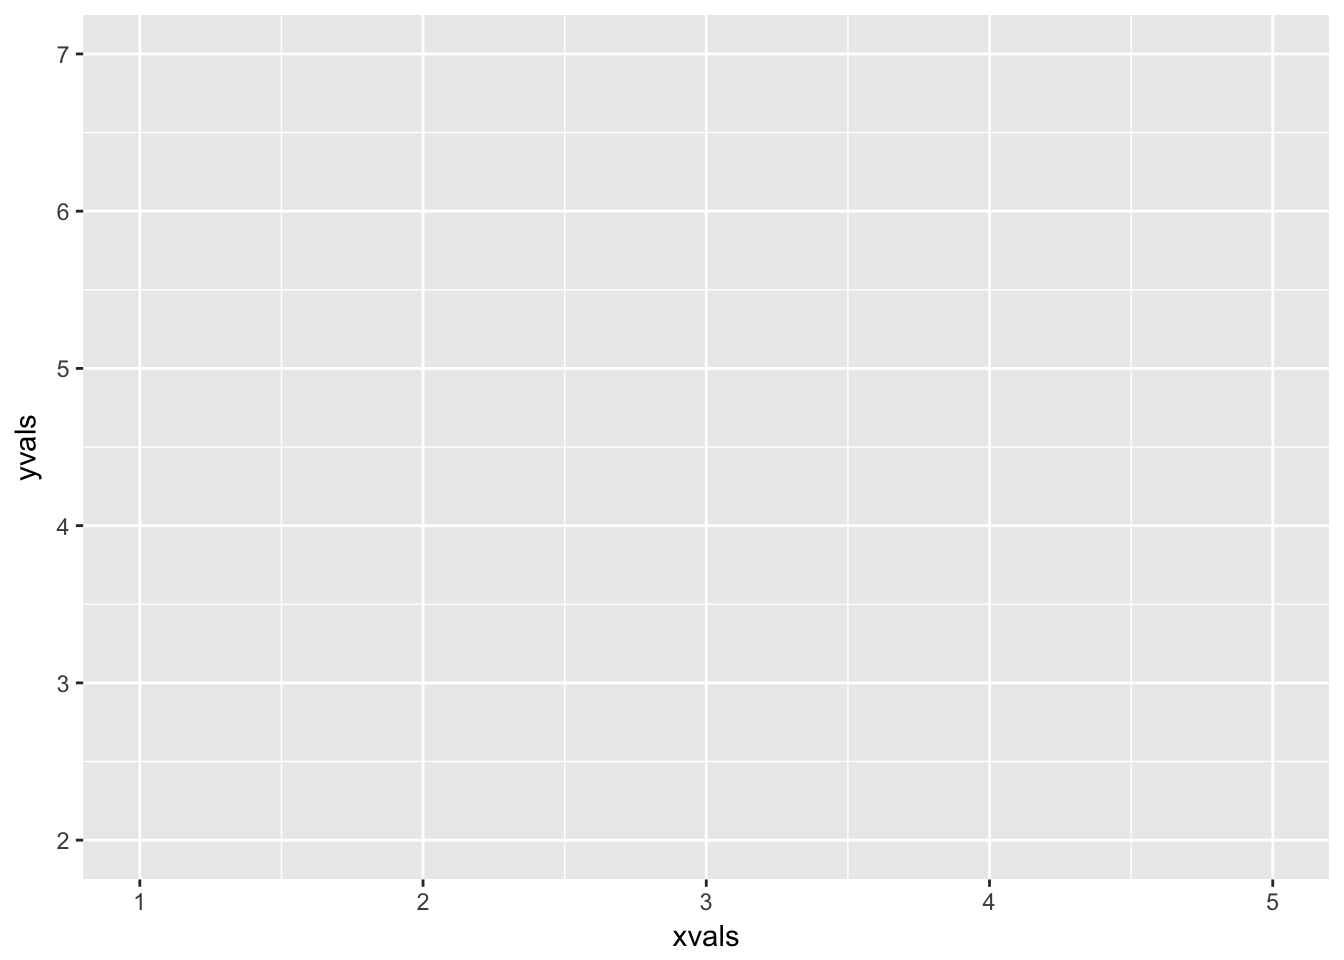
\includegraphics[width=0.5\linewidth]{r-notes_files/figure-latex/blank-ggplot-1} 

}

\caption{A ggplot2 plot without geoms.}\label{fig:blank-ggplot}
\end{figure}

The plot is blank! Why is this? Well, although \texttt{ggplot()} has
been told what values are to be represented on the plot and where they
might go, it has not yet been told how they should be shaped: it has not
been told their \emph{geometry}, you might say. We can add a geometry to
\texttt{p} to get a picture (see Figure \ref{fig:pointsggplot}:

\begin{Shaded}
\begin{Highlighting}[]
\KeywordTok{print}\NormalTok{(p +}\StringTok{ }\KeywordTok{geom_point}\NormalTok{())}
\end{Highlighting}
\end{Shaded}

\begin{figure}

{\centering 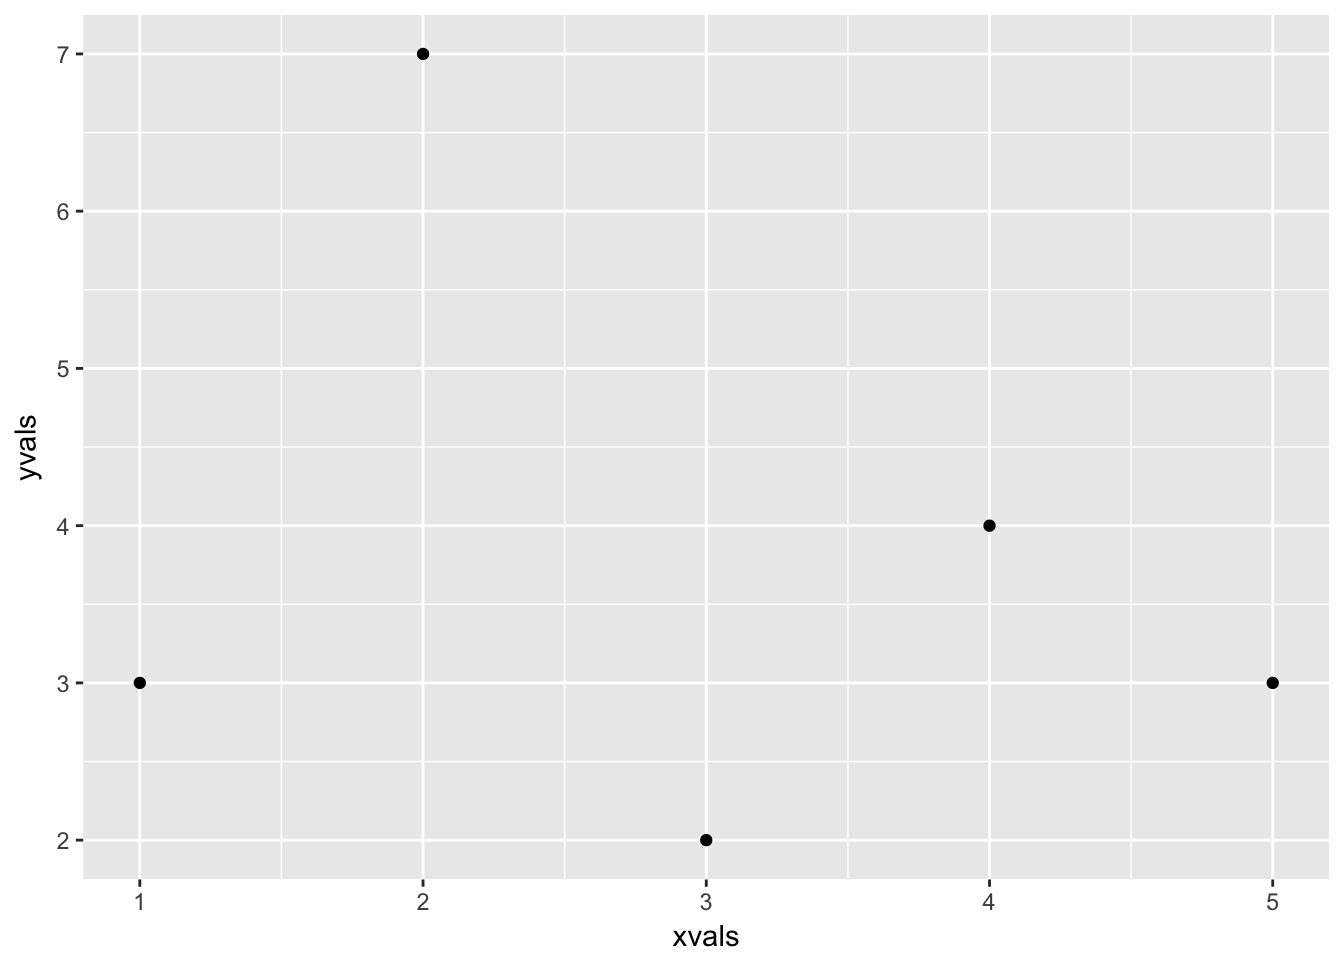
\includegraphics[width=0.5\linewidth]{r-notes_files/figure-latex/pointsggplot-1} 

}

\caption{A ggplot2 plot with the point geom.}\label{fig:pointsggplot}
\end{figure}

The geometry determines a lot about the look of the plot. In order to
have the points connected by lines we could add \texttt{geom\_line()}
(see Figure \ref{fig:pointslinesggplot}:

\begin{Shaded}
\begin{Highlighting}[]
\KeywordTok{print}\NormalTok{(p +}\StringTok{ }\KeywordTok{geom_point}\NormalTok{() +}\StringTok{ }\KeywordTok{geom_line}\NormalTok{())}
\end{Highlighting}
\end{Shaded}

\begin{figure}

{\centering 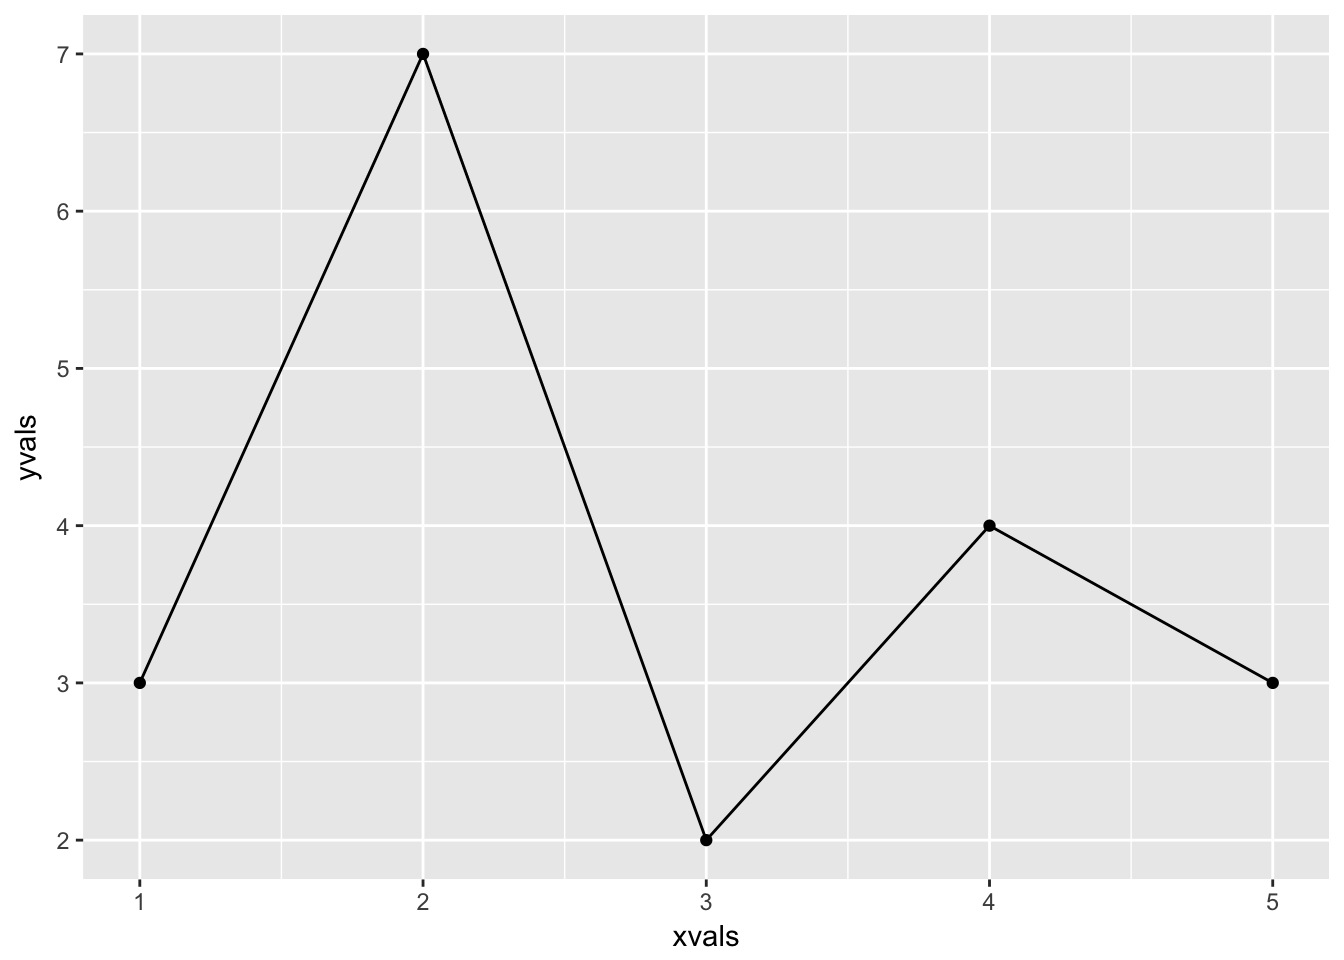
\includegraphics[width=0.5\linewidth]{r-notes_files/figure-latex/pointslinesggplot-1} 

}

\caption{A ggplot2 plot with point and line geoms.}\label{fig:pointslinesggplot}
\end{figure}

We'll choose a scatterplot with connecting lines for our graph of the
sequence. With a little more work we can get nice labels for the x and
y-axes, and a title for the graph. Our \texttt{collatz()} function now
looks like:

\begin{Shaded}
\begin{Highlighting}[]
\NormalTok{collatz <-}\StringTok{ }\NormalTok{function(n, }\DataTypeTok{limit =} \DecValTok{10000}\NormalTok{) \{}
  \CommentTok{# record initial numer because will change n}
  \NormalTok{initial <-}\StringTok{ }\NormalTok{n  }
  \NormalTok{numbers <-}\StringTok{ }\KeywordTok{numeric}\NormalTok{(limit)}
  \NormalTok{counter <-}\StringTok{ }\DecValTok{0}
  \NormalTok{while ( n >}\StringTok{ }\DecValTok{1} \NormalTok{&}\StringTok{ }\NormalTok{counter <}\StringTok{ }\NormalTok{limit) \{}
    \NormalTok{counter <-}\StringTok{ }\NormalTok{counter +}\StringTok{ }\DecValTok{1}
    \NormalTok{numbers[counter] <-}\StringTok{ }\NormalTok{n}
    \NormalTok{n <-}\StringTok{ }\KeywordTok{collatzRule}\NormalTok{(n)}
  \NormalTok{\}}
  \NormalTok{howMany <-}\StringTok{ }\KeywordTok{min}\NormalTok{(counter, limit)}
  \KeywordTok{cat}\NormalTok{(}\StringTok{"The Collatz sequence has "}\NormalTok{, howMany, }\StringTok{" elements.}\CharTok{\textbackslash{}n}\StringTok{"}\NormalTok{, }\DataTypeTok{sep =} \StringTok{""}\NormalTok{)}
  \NormalTok{show <-}\StringTok{ }\KeywordTok{readline}\NormalTok{(}\StringTok{"Do you want to see it (y/n)?  "}\NormalTok{)}
  \NormalTok{if ( show ==}\StringTok{ "y"} \NormalTok{) \{}
    \KeywordTok{print}\NormalTok{(numbers[}\DecValTok{1}\NormalTok{:howMany])}
  \NormalTok{\}}
  \CommentTok{# use initial value to make plot title:}
  \NormalTok{plotTitle <-}\StringTok{ }\KeywordTok{paste0}\NormalTok{(}\StringTok{"Collatz Sequence for n = "}\NormalTok{, initial)}
  \CommentTok{# make the plot}
  \NormalTok{p <-}\StringTok{ }\KeywordTok{ggplot}\NormalTok{(}\DataTypeTok{mapping =} \KeywordTok{aes}\NormalTok{(}\DataTypeTok{x =} \NormalTok{steps, }\DataTypeTok{y =} \NormalTok{number[}\DecValTok{1}\NormalTok{:howMany])) +}
\StringTok{    }\KeywordTok{geom_point}\NormalTok{() +}\StringTok{ }\KeywordTok{geom_line}\NormalTok{() +}
\StringTok{    }\KeywordTok{labs}\NormalTok{( }\DataTypeTok{x =} \StringTok{"Step"}\NormalTok{, }\DataTypeTok{y =} \StringTok{"Collatz Value at Step"}\NormalTok{,}
          \DataTypeTok{title =} \NormalTok{plotTitle)}
  \CommentTok{# print it to the Plot Window}
  \KeywordTok{print}\NormalTok{(p)}
\NormalTok{\}}
\end{Highlighting}
\end{Shaded}

Try this version a few times, like so:

\begin{Shaded}
\begin{Highlighting}[]
\KeywordTok{collatz}\NormalTok{(}\DecValTok{257}\NormalTok{)}
\end{Highlighting}
\end{Shaded}

It's quite remarkable how much the sequence can rise and fall before
hitting 1.

One final consideration is validation\index{validation} of user-input.
we don't want the user to get strange errors if she fails to enter a
number worth looking at---a whole number that is greater than 1.

One possible approach is to attempt to coerce the user's input into an
integer, using the \texttt{as.integer()}
function:\index{R-functions!as.integer()@\texttt{as.integer()}}

\begin{Shaded}
\begin{Highlighting}[]
\KeywordTok{as.integer}\NormalTok{(}\FloatTok{3.6}\NormalTok{) }\CommentTok{# will round to nearest integer}
\end{Highlighting}
\end{Shaded}

\begin{verbatim}
## [1] 3
\end{verbatim}

\begin{Shaded}
\begin{Highlighting}[]
\KeywordTok{as.integer}\NormalTok{(}\StringTok{"4"}\NormalTok{) }\CommentTok{# will convert string to number 4}
\end{Highlighting}
\end{Shaded}

\begin{verbatim}
## [1] 4
\end{verbatim}

\begin{Shaded}
\begin{Highlighting}[]
\KeywordTok{as.integer}\NormalTok{(}\StringTok{"4.3"}\NormalTok{) }\CommentTok{# will convert AND round}
\end{Highlighting}
\end{Shaded}

\begin{verbatim}
## [1] 4
\end{verbatim}

\begin{Shaded}
\begin{Highlighting}[]
\KeywordTok{as.integer}\NormalTok{(}\StringTok{"hello"}\NormalTok{) }\CommentTok{# cannot convert to integer}
\end{Highlighting}
\end{Shaded}

\begin{verbatim}
## Warning: NAs introduced by coercion
\end{verbatim}

\begin{verbatim}
## [1] NA
\end{verbatim}

In the last example, the result is \texttt{NA}, and a cryptic warning
was issued. In order to keep the warning from the user, we should wrap
any call to \texttt{as.integer()} in the suppressWarnings()` function.

Let's try out a piece of code that implements validation:

\begin{Shaded}
\begin{Highlighting}[]
\NormalTok{n <-}\StringTok{ }\NormalTok{-}\DecValTok{2}
\NormalTok{n <-}\StringTok{ }\KeywordTok{suppressWarnings}\NormalTok{(}\KeywordTok{as.integer}\NormalTok{(n))}
\NormalTok{isValid <-}\StringTok{ }\NormalTok{!}\KeywordTok{is.na}\NormalTok{(n) &&}\StringTok{ }\NormalTok{n >}\StringTok{ }\DecValTok{1}
  \NormalTok{if (!isValid ) \{}
    \KeywordTok{stop}\NormalTok{(}\StringTok{"Need an integer bigger than 1.  Try again."}\NormalTok{)}
  \NormalTok{\}}
\end{Highlighting}
\end{Shaded}

\begin{verbatim}
## Error: Need an integer bigger than 1.  Try again.
\end{verbatim}

The \texttt{stop()} \index{R-functions!stop()@\texttt{stop()}}function
throws a true error that prevents any further code from being executed,
but allows us to write a custom, friendly error-message. The goal of
validation is for the user to receive clear and helpful error messages,
rather than obscure, technical messages from the depths of R.

The final version of the \texttt{collatz()} function appears below.

\begin{Shaded}
\begin{Highlighting}[]
\NormalTok{collatz <-}\StringTok{ }\NormalTok{function(n, }\DataTypeTok{limit =} \DecValTok{10000}\NormalTok{) \{}
  \CommentTok{# record initial numer because will change n}
  \NormalTok{initial <-}\StringTok{ }\NormalTok{n }
  \CommentTok{# validation:}
  \NormalTok{n <-}\StringTok{ }\KeywordTok{suppressWarnings}\NormalTok{(}\KeywordTok{as.integer}\NormalTok{(n))}
  \NormalTok{isValid <-}\StringTok{ }\NormalTok{!}\KeywordTok{is.na}\NormalTok{(n) &&}\StringTok{ }\NormalTok{n >}\StringTok{ }\DecValTok{1}
  \NormalTok{if (!isValid ) \{}
    \KeywordTok{stop}\NormalTok{(}\StringTok{"Need an integer bigger than 1.  Try again."}\NormalTok{)}
  \NormalTok{\}}
  \NormalTok{numbers <-}\StringTok{ }\KeywordTok{numeric}\NormalTok{(limit)}
  \NormalTok{counter <-}\StringTok{ }\DecValTok{0}
  \NormalTok{while ( n >}\StringTok{ }\DecValTok{1} \NormalTok{&}\StringTok{ }\NormalTok{counter <}\StringTok{ }\NormalTok{limit) \{}
    \NormalTok{counter <-}\StringTok{ }\NormalTok{counter +}\StringTok{ }\DecValTok{1}
    \NormalTok{numbers[counter] <-}\StringTok{ }\NormalTok{n}
    \NormalTok{n <-}\StringTok{ }\KeywordTok{collatzRule}\NormalTok{(n)}
  \NormalTok{\}}
  \NormalTok{howMany <-}\StringTok{ }\KeywordTok{min}\NormalTok{(counter, limit)}
  \KeywordTok{cat}\NormalTok{(}\StringTok{"The Collatz sequence has "}\NormalTok{, howMany, }\StringTok{" elements.}\CharTok{\textbackslash{}n}\StringTok{"}\NormalTok{, }\DataTypeTok{sep =} \StringTok{""}\NormalTok{)}
  \NormalTok{show <-}\StringTok{ }\KeywordTok{readline}\NormalTok{(}\StringTok{"Do you want to see it (y/n)?  "}\NormalTok{)}
  \NormalTok{if ( show ==}\StringTok{ "y"} \NormalTok{) \{}
    \KeywordTok{print}\NormalTok{(numbers[}\DecValTok{1}\NormalTok{:howMany])}
  \NormalTok{\}}
  \NormalTok{plotTitle <-}\StringTok{ }\KeywordTok{paste0}\NormalTok{(}\StringTok{"Collatz Sequence for n = "}\NormalTok{, initial)}
  \NormalTok{p <-}\StringTok{ }\KeywordTok{ggplot}\NormalTok{(}\DataTypeTok{mapping =} \KeywordTok{aes}\NormalTok{(}\DataTypeTok{x =} \NormalTok{steps, }\DataTypeTok{y =} \NormalTok{number[}\DecValTok{1}\NormalTok{:howMany])) +}
\StringTok{    }\KeywordTok{geom_point}\NormalTok{() +}\StringTok{ }\KeywordTok{geom_line}\NormalTok{() +}
\StringTok{    }\KeywordTok{labs}\NormalTok{( }\DataTypeTok{x =} \StringTok{"Step"}\NormalTok{, }\DataTypeTok{y =} \StringTok{"Collatz Value at Step"}\NormalTok{,}
          \DataTypeTok{title =} \NormalTok{plotTitle)}
  \KeywordTok{print}\NormalTok{(p)}
\NormalTok{\}}
\end{Highlighting}
\end{Shaded}

\newpage

\section*{Glossary}\label{glossary-2}
\addcontentsline{toc}{section}{Glossary}

\begin{description}
\item[Flow Control \index{flow control}]
The collection of devices within a programming language that allow the
computer to make decisions and to repeat tasks.
\item[Condition \index{condition}]
A Boolean expression that commences an \texttt{if} or \texttt{while}
statement. If the condition evaluates to \texttt{TRUE}, then the code in
the body of the statement will be executed. Otherwise the code will be
ignored.
\item[Index Variable \index{index variable}]
The variable in a \texttt{for} loop that takes on each of the values of
the iterable in succession.
\item[Iterable \index{iterable}]
The vector that provides the sequence of values for the index variable
in a \texttt{for} loop.
\item[Validation \index{validation}]
The process of checking user input and rejecting it---usually with
helpful suggestions---if it is not of the correct form.
\end{description}

\newpage

\section*{Exercises}\label{exercises-2}
\addcontentsline{toc}{section}{Exercises}

\begin{center}
\includegraphics[width=0.5\linewidth]{images/thinking} \end{center}

\begin{enumerate}
\def\labelenumi{\arabic{enumi}.}
\item
  The \emph{absolute value} of a number \(x\) is defined to be the
  number \(x\) itself if \(x \ge 0\), whereas it is the opposite of
  \(x\) if \(x < 0\). Thus:

  \begin{itemize}
  \tightlist
  \item
    the absolute value of 3 is 3;
  \item
    the absolute value of -3 is -(-3), which is 3;
  \item
    the absolute value of -5.7 is -(-5.7), which is 5.7
  \item
    the absolute value of 0 is 0.
  \end{itemize}

  The absolute value is important enough that R provides the
  \texttt{abs()}\index{R-functions!abs()@\texttt{abs()}} function to
  compute it. Thus:

\begin{Shaded}
\begin{Highlighting}[]
\KeywordTok{abs}\NormalTok{(-}\FloatTok{3.7}\NormalTok{)}
\end{Highlighting}
\end{Shaded}

\begin{verbatim}
## [1] 3.7
\end{verbatim}

  Write a function called \texttt{absolute()} that computes the absolute
  value of any given number \texttt{x}. Your code should make no
  reference to R's \texttt{abs()}.

  \textbf{Small Bonus}: Write the function so that it follows the
  vector-in, vector-out principle, that is: when it is given a vector of
  numbers it returns the vector of their absolute values, like this:

\begin{Shaded}
\begin{Highlighting}[]
\NormalTok{vec <-}\StringTok{ }\KeywordTok{c}\NormalTok{(-}\DecValTok{3}\NormalTok{, }\DecValTok{5}\NormalTok{, -}\FloatTok{2.7}\NormalTok{)}
\KeywordTok{absolute}\NormalTok{(vec)}
\end{Highlighting}
\end{Shaded}

\begin{verbatim}
## [1] 3.0 5.0 2.7
\end{verbatim}
\item
  Write a function called \texttt{pattern()} that, when given any
  character \(x\) and any positive number \(n\), will print the
  following pattern to the console:

  \begin{itemize}
  \tightlist
  \item
    a line with just one \(x\),
  \item
    another line with two \(x\)'s,
  \item
    another line with three \(x\)'s,
  \item
    and so on until \ldots{}
  \item
    a line with \(n\) \(x\)'s, and then
  \item
    another line with \(n-1\) \(x\)'s,
  \item
    and so on until \ldots{}
  \item
    a line with just one \(x\).
  \end{itemize}

  Thus when the character is \texttt{*} and \texttt{n} is 5, the output
  would look like this:

\begin{verbatim}
## *
## **
## ***
## ****
## *****
## ****
## ***
## **
## *
\end{verbatim}

  The function should take two arguments:

  \begin{itemize}
  \tightlist
  \item
    \texttt{char}: the character to repeat. The default value should be
    \texttt{"*"}.
  \item
    \texttt{n}: the number of characters in the longest, middle line.
    The default value should be 3.
  \end{itemize}
\item
  Write a function called \texttt{beerTune()} that prints out the
  complete lyrics to the song \emph{Ninety-Nine Bottles of Beer on the
  Wall}. You'll recall that the song goes like this:

  \begin{quote}
  99 bottles of beer on the wall,
  \end{quote}

  \begin{quote}
  99 bottles of beer!
  \end{quote}

  \begin{quote}
  Take one down and pass it around:
  \end{quote}

  \begin{quote}
  98 bottles of beer on the wall.
  \end{quote}

  \begin{quote}
  98 bottles of beer on the wall,
  \end{quote}

  \begin{quote}
  98 bottles of beer!
  \end{quote}

  \begin{quote}
  Take one down and pass it around:
  \end{quote}

  \begin{quote}
  \ldots{}
  \end{quote}

  \begin{quote}
  1 bottle of beer on the wall.
  \end{quote}

  \begin{quote}
  1 bottle of beer!
  \end{quote}

  \begin{quote}
  Take it down and pass it around:
  \end{quote}

  \begin{quote}
  No more bottles of beer on the wall.
  \end{quote}

  Make sure to get the lyrics exactly right. For example, it's ``1
  bottle'', not ``1 bottles''.
\item
  Recall the function \texttt{madhavaPI()} from Section
  \ref{default-arguments}. Use this function to write a function called
  \texttt{madhavaGraph()} that will do the following: given a number
  \(n\), the function uses \textbf{ggplot2} to produce a line graph of
  the first \(n\) approximations to \(\pi\) using the initial terms of
  the Madhava series. The plot should be a line graph similar to the one
  produced by the \texttt{collatz()} functions from this Chapter. The
  function should take a single argument \texttt{n}, whose default value
  is 10. It should validate the input: if the number entered is not at
  least 1, then the function should throw an error and explain to the
  user that the he/she must enter a positive number.

  Here is an example of how the function should work:

\begin{Shaded}
\begin{Highlighting}[]
\KeywordTok{madhavaGraph}\NormalTok{(}\DataTypeTok{n =} \NormalTok{-}\DecValTok{3}\NormalTok{)}
\end{Highlighting}
\end{Shaded}

\begin{verbatim}
## You need to enter a positive integer.  Try again!
\end{verbatim}

  Here is another example:

\begin{Shaded}
\begin{Highlighting}[]
\KeywordTok{madhavaGraph}\NormalTok{(}\DataTypeTok{n =} \DecValTok{20}\NormalTok{)}
\end{Highlighting}
\end{Shaded}

  The output should be as in Figure \ref{fig:madhavaGraph}.

  \begin{figure}

  {\centering 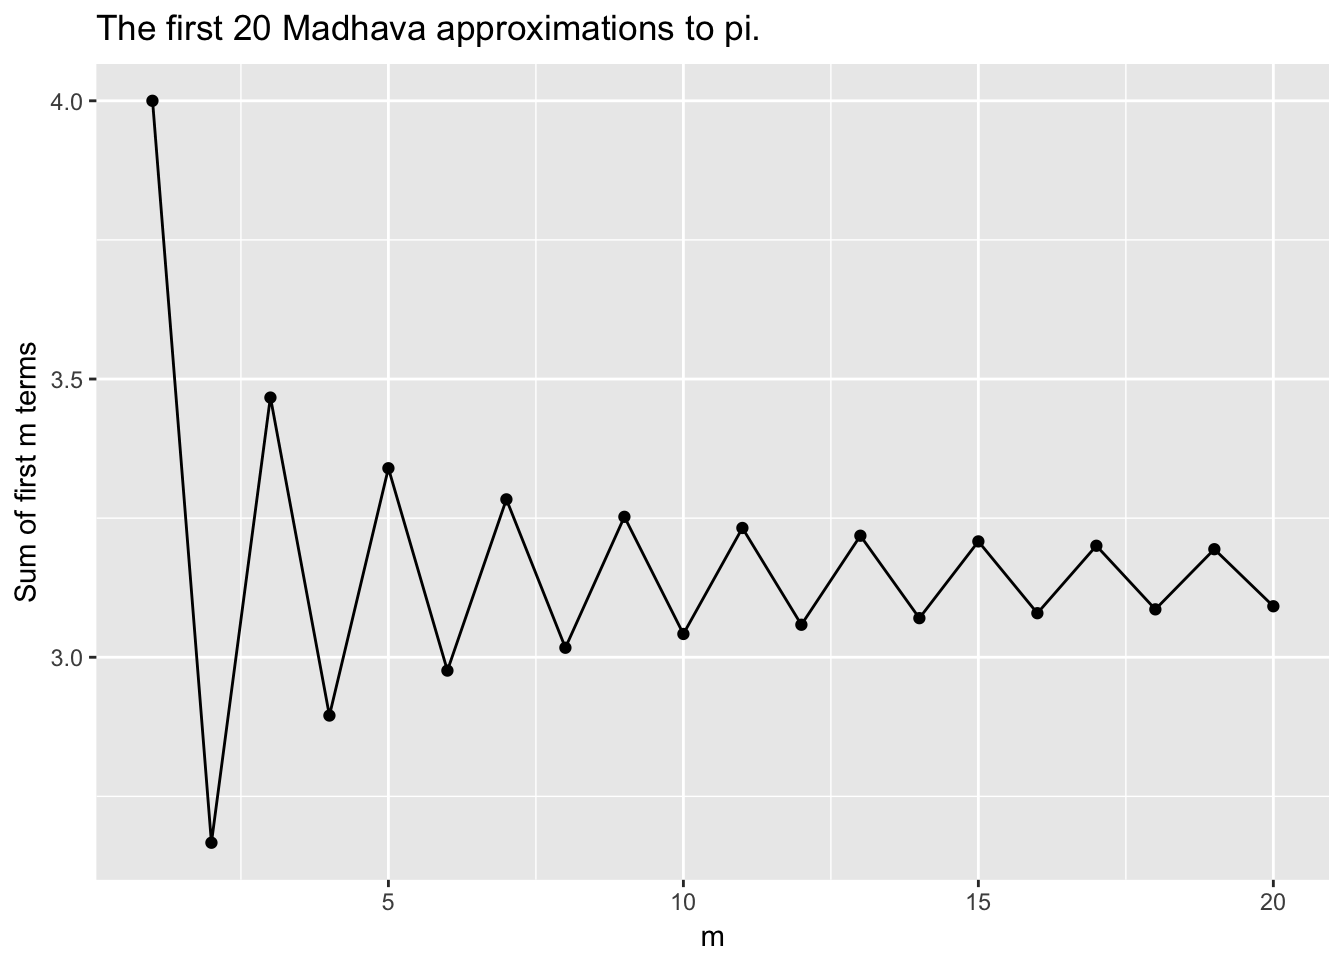
\includegraphics[width=0.5\linewidth]{r-notes_files/figure-latex/madhavaGraph-1} 

  }

  \caption{This is how the output of the     madhavaGraph function should look.}\label{fig:madhavaGraph}
  \end{figure}
\item
  \textbf{The Subtraction Game.} In this game there are two players, A
  and B, and a pile of \(n\) pebbles. The players take turns removing
  pebbles from the pile. On each turn, a player can take either one or
  two pebbles. The players who takes the last pebble wins the game.

  It turns out that one of the players has a winning strategy. If the
  initial number of pebbles is a multiple of 3, then player who goes
  second has a winning strategy, whereas if the initial number of
  pebbles is not a multiple of 3 then the player who goes second has the
  winning strategy.

  The idea for the winning strategy comes from the following
  observations:

  \begin{itemize}
  \tightlist
  \item
    If there are 3 pebbles left and it's the other player's turn, then
    you will win. Why? Because after the other player removes pebbles
    there will be either 1 or 2 pebbles left. In either case you will be
    able to take the last pebble.
  \item
    If there are 6 pebbles left and it's the other player's turn, then
    you will win. Why? Because after the other player removes pebbles
    there will be either 4 or 5 pebbles left. In either case on your
    turn you will be able to reduce the number of pebbles to 3. The game
    is now in the state of the previous bullet item, where we know that
    you will win.
  \item
    If there are 9 pebbles left and it's the other player's turn, then
    you will win. Why? Because after the other player removes pebbles
    there will be either 7 or 8 pebbles left. In either case on your
    turn you will be able to reduce the number of pebbles to 6. The game
    is now in the state of the previous bullet item, where we know that
    you will win.
  \item
    And so on, for 12 left, 15 left, 18 left, etc.
  \end{itemize}

  As long as the number of pebbles left is a multiple of 3 and it's the
  other player's turn, you will win!

  In this problem you task is to write a function called
  \texttt{subtraction()} will play the Subtraction Game with a user. The
  function should take two parameters:

  \begin{itemize}
  \tightlist
  \item
    \texttt{n}: the number of pebbles to begin with. The default value
    should be 12.
  \item
    \texttt{userFirst}: a logical parameter that indicates whether the
    user or the computer plays first. The default value should be
    \texttt{TRUE}, meaning that the user goes first.
  \end{itemize}

  Each time the computer plays it should announce how many pebbles it
  removed, and how many are left. When there are no pebbles left the
  computer should say who won and quit the function.

  The function should play optimally for the computer:

  \begin{itemize}
  \tightlist
  \item
    if at the outset the computer has a winning strategy, then the
    computer should follow it and win.
  \item
    if at the outset the user has a winning strategy then the computer
    watch for opportunities to win if the user departs from her winning
    strategy.
  \end{itemize}
\end{enumerate}

\chapter{Turtle Graphics}\label{turtle}

\begin{figure}[!h]

{\centering 
\includegraphics[width=0.9\linewidth]{images/xkcd-turtles} 

}

\caption{Turtles, by xkcd.}\label{fig:xkcd-turtles}
\end{figure}

In this chapter we will practice our knowledge of R---and of basic
programming concepts---in the context of a special R-package for
graphics: package \textbf{TurtleGraphics} \citep{R-TurtleGraphics}. Many
of the examples from this Chapter are drawn from the Vignette for the
package.\footnote{Turtle Graphics itself is not original to R. It was
  developed in the 1960's by Seymour Papert for use in the LOGO
  programming language. LOGO is a general-purpose programming language
  but has been primarily used to teach programming concepts to children.
  Nevertheless, grown-ups enjoy playing with Turtle Graphics so much
  that implementations of the system are now found in several major
  ``professional-grade'' programming languages. For more information
  about Turtle Graphics, consult \citet{Papert1993}.}

\newpage

\section{Basic Movements}\label{basic-movements}

First, we begin by loading the package:

\begin{Shaded}
\begin{Highlighting}[]
\KeywordTok{library}\NormalTok{(TurtleGraphics)}
\end{Highlighting}
\end{Shaded}

In order to create a Turtle Graphics scenario, call the function
\texttt{turtle\_init()}. You get the plot shown in Figure
\ref{fig:initial-turtle}.

\begin{Shaded}
\begin{Highlighting}[]
\KeywordTok{turtle_init}\NormalTok{()}
\end{Highlighting}
\end{Shaded}

\begin{figure}

{\centering 
\includegraphics[width=0.5\linewidth]{r-notes_files/figure-latex/initial-turtle-1} 

}

\caption{Initialized Turtle}\label{fig:initial-turtle}
\end{figure}

By default the turtle is positioned in the middle of a square of
dimensions 100 units by 100 units. (These dimensions can be changed, as
we will see later on.)

You can get the turtle's position at any time:

\begin{Shaded}
\begin{Highlighting}[]
\KeywordTok{turtle_getpos}\NormalTok{()}
\end{Highlighting}
\end{Shaded}

\begin{verbatim}
##  x  y 
## 50 50 
\end{verbatim}

The turtle also begins facing North. This is considered to be angle 0,
as you can tell by asking for the current angle of the turtle:

\begin{Shaded}
\begin{Highlighting}[]
\KeywordTok{turtle_getangle}\NormalTok{()}
\end{Highlighting}
\end{Shaded}

\begin{verbatim}
## angle 
##     0 
\end{verbatim}

Now let's make the turtle move. If you are following along on your own
computer, it's best to run the lines of code one at a time, so you can
see the effect of each command. (If you run multiples lines, you'll only
see the graph produced by the final line.)

\begin{Shaded}
\begin{Highlighting}[]
\KeywordTok{turtle_forward}\NormalTok{(}\DataTypeTok{dist =} \DecValTok{30}\NormalTok{)}
\KeywordTok{turtle_backward}\NormalTok{(}\DataTypeTok{dist =} \DecValTok{10}\NormalTok{)}
\end{Highlighting}
\end{Shaded}

\begin{figure}

{\centering 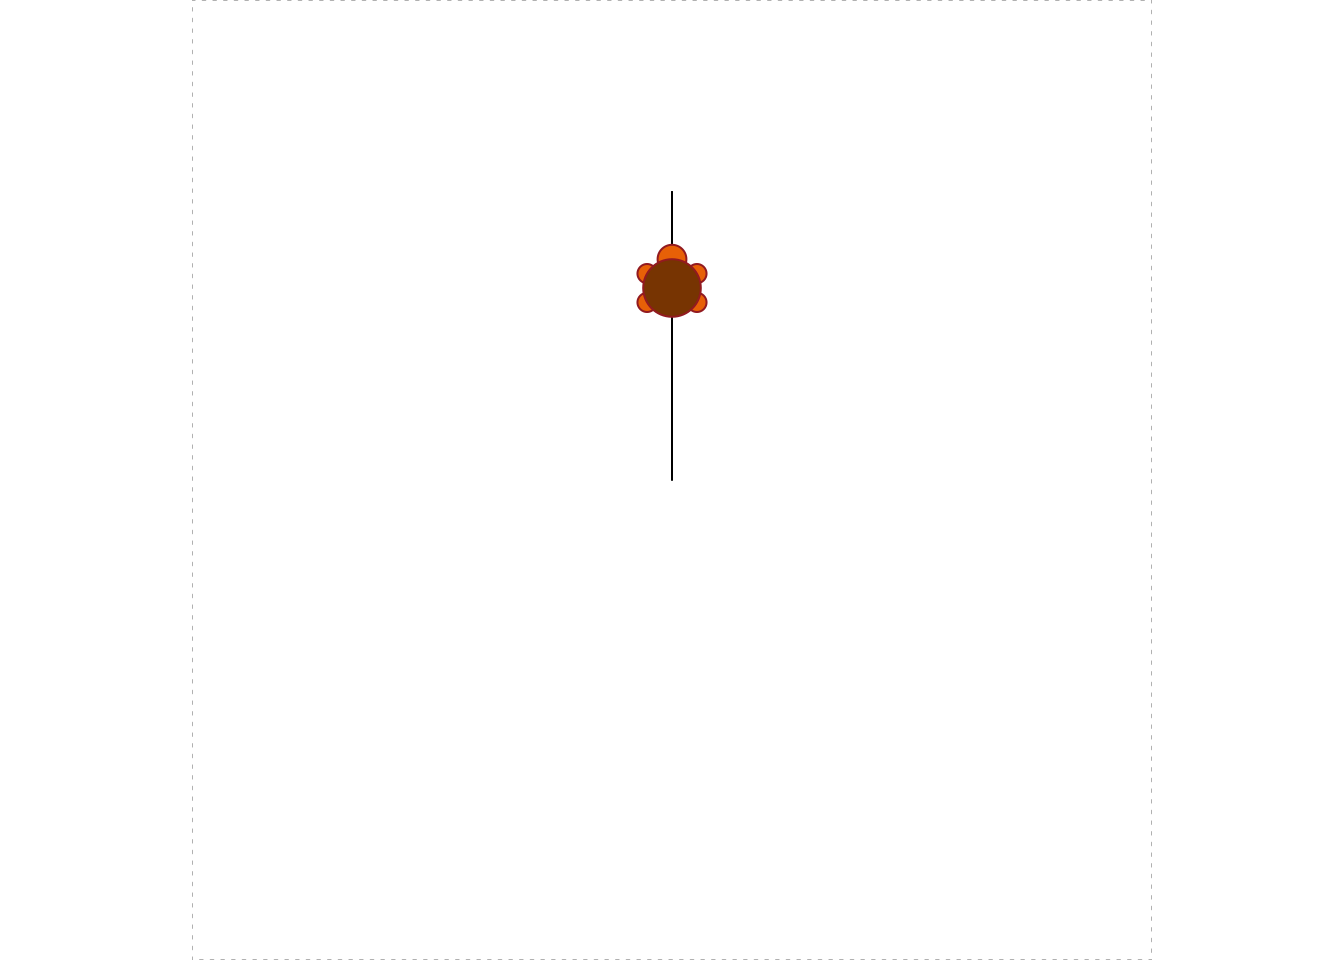
\includegraphics[width=0.5\linewidth]{r-notes_files/figure-latex/first-movement-1} 

}

\caption{First Movements}\label{fig:first-movement}
\end{figure}

The result appears in Figure \ref{fig:first-movement}. Next we'll add a
little triangle:

\begin{Shaded}
\begin{Highlighting}[]
\KeywordTok{turtle_right}\NormalTok{(}\DecValTok{90}\NormalTok{)}
\KeywordTok{turtle_forward}\NormalTok{(}\DecValTok{10}\NormalTok{)}
\KeywordTok{turtle_left}\NormalTok{(}\DataTypeTok{angle =} \DecValTok{135}\NormalTok{)}
\KeywordTok{turtle_forward}\NormalTok{(}\FloatTok{14.14}\NormalTok{)}
\KeywordTok{turtle_left}\NormalTok{(}\DataTypeTok{angle =} \DecValTok{90}\NormalTok{)}
\KeywordTok{turtle_forward}\NormalTok{(}\FloatTok{14.14}\NormalTok{)}
\KeywordTok{turtle_left}\NormalTok{(}\DataTypeTok{angle =} \DecValTok{135}\NormalTok{)}
\KeywordTok{turtle_forward}\NormalTok{(}\DecValTok{10}\NormalTok{)}
\end{Highlighting}
\end{Shaded}

\begin{figure}

{\centering 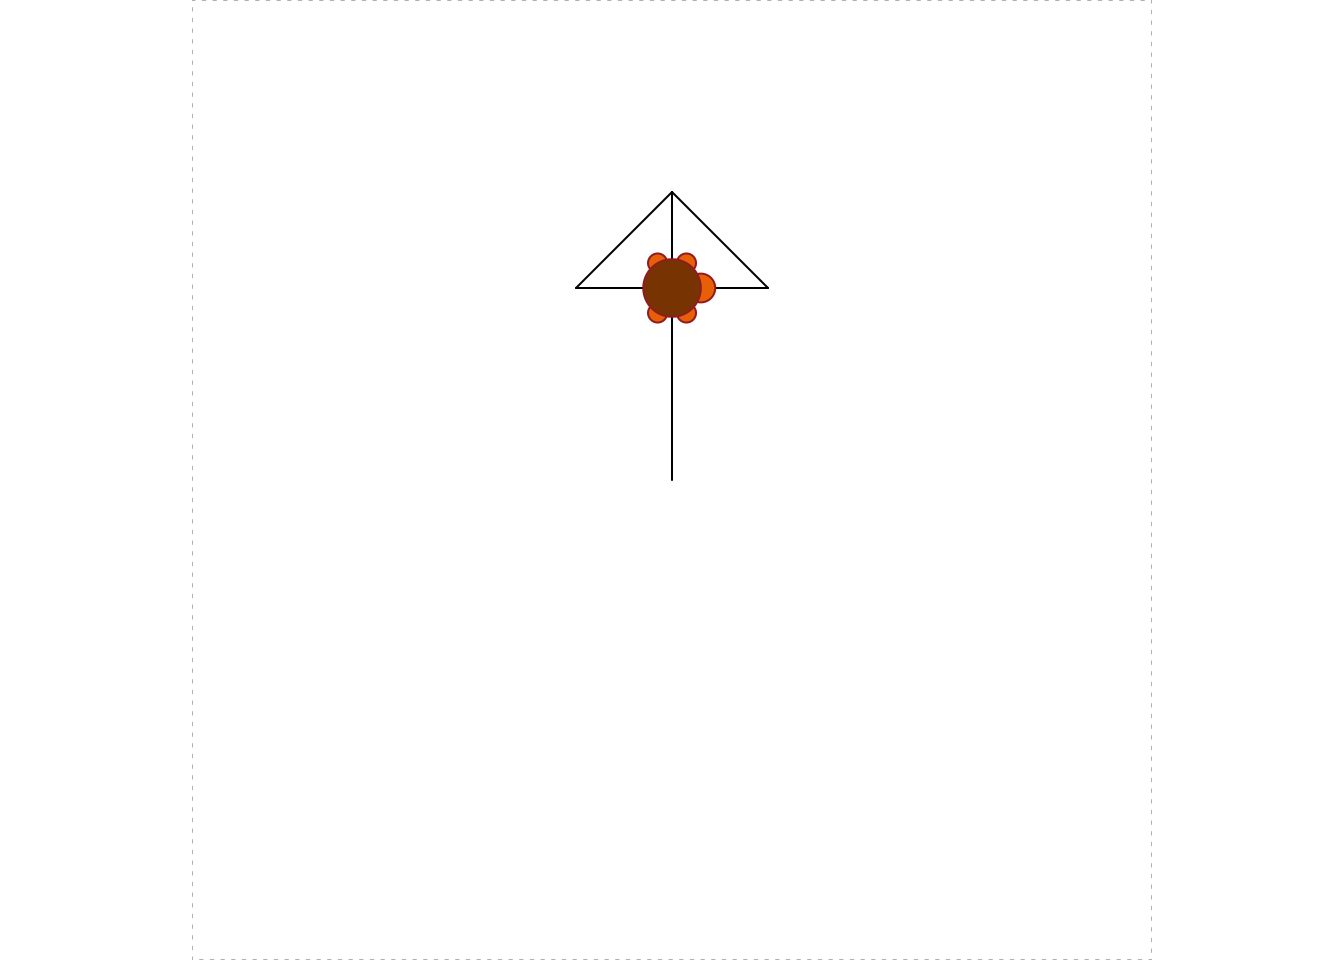
\includegraphics[width=0.5\linewidth]{r-notes_files/figure-latex/add-triangle-1} 

}

\caption{Adding a Triangle}\label{fig:add-triangle}
\end{figure}

You can see the triangle in Figure \ref{fig:add-triangle}.

The turtle is set in the ``down'' position, so that it leaves a trace
out the path that it follows. You can avoid the trace by pulling the
turtle ``up'' with \texttt{turtle\_up()}. Whenever you want to restore
the tracing, call \texttt{turtle\_down()}. See Figure \ref{fig:up-down}
for the results of the following code.

\begin{Shaded}
\begin{Highlighting}[]
\KeywordTok{turtle_up}\NormalTok{()  }\CommentTok{# stop tracing}
\KeywordTok{turtle_right}\NormalTok{(}\DataTypeTok{angle =} \DecValTok{90}\NormalTok{)}
\KeywordTok{turtle_forward}\NormalTok{(}\DataTypeTok{dist =} \DecValTok{10}\NormalTok{)}
\KeywordTok{turtle_right}\NormalTok{(}\DataTypeTok{angle =} \DecValTok{90}\NormalTok{)}
\KeywordTok{turtle_forward}\NormalTok{(}\DataTypeTok{dist =} \DecValTok{17}\NormalTok{)}
\KeywordTok{turtle_down}\NormalTok{()  }\CommentTok{# start tracing again}
\KeywordTok{turtle_left}\NormalTok{(}\DataTypeTok{angle =} \DecValTok{180}\NormalTok{)}
\KeywordTok{turtle_forward}\NormalTok{(}\DataTypeTok{dist =} \DecValTok{34}\NormalTok{)}
\end{Highlighting}
\end{Shaded}

\begin{figure}

{\centering 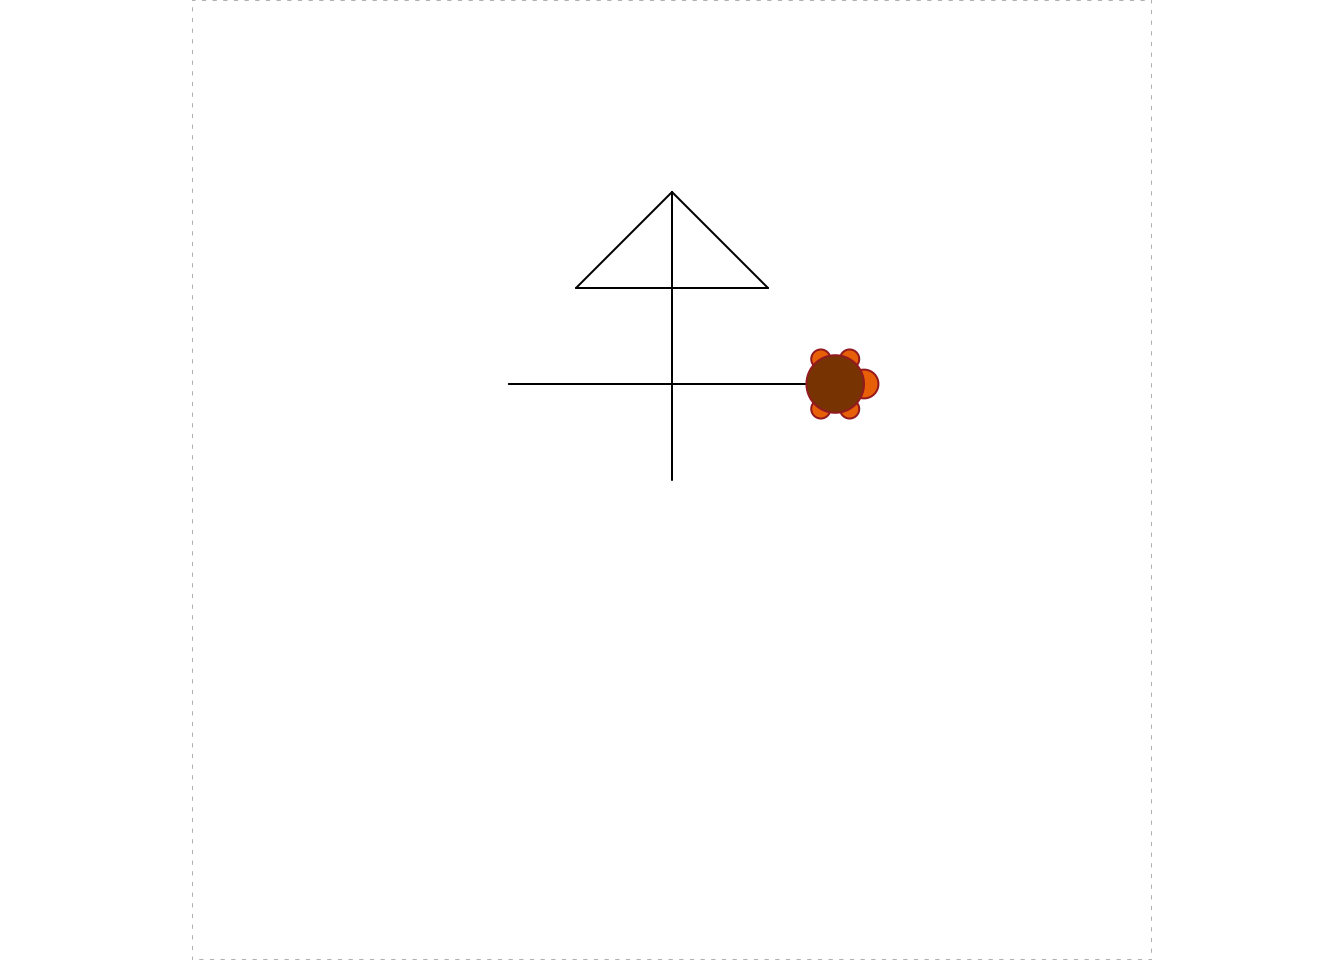
\includegraphics[width=0.5\linewidth]{r-notes_files/figure-latex/up-down-1} 

}

\caption{We moved the turtle around in the up position, then put the turtle down and traced out a line segment.}\label{fig:up-down}
\end{figure}

You can change the color of the lines your turtle draws:

\begin{Shaded}
\begin{Highlighting}[]
\KeywordTok{turtle_col}\NormalTok{(}\DataTypeTok{col =} \StringTok{"green"}\NormalTok{)}
\end{Highlighting}
\end{Shaded}

In R here are many, many colors to choose from, and 657 of them even
have names. To view them, use:= the \texttt{colors()} function:
\index{R-functions!colors()@\texttt{colors()}}

\begin{Shaded}
\begin{Highlighting}[]
\KeywordTok{colors}\NormalTok{()}
\end{Highlighting}
\end{Shaded}

You can also hide your turtle, and show it again any time you like. See
Figure \ref{fig:hide-show} for the results of the following code.

\begin{Shaded}
\begin{Highlighting}[]
\KeywordTok{turtle_hide}\NormalTok{()}
\KeywordTok{turtle_left}\NormalTok{(}\DataTypeTok{angle =} \DecValTok{150}\NormalTok{)}
\KeywordTok{turtle_forward}\NormalTok{(}\DataTypeTok{dist =} \DecValTok{20}\NormalTok{)}
\KeywordTok{turtle_left}\NormalTok{(}\DataTypeTok{angle =} \DecValTok{60}\NormalTok{)}
\KeywordTok{turtle_forward}\NormalTok{(}\DataTypeTok{dist =} \DecValTok{20}\NormalTok{)}
\KeywordTok{turtle_show}\NormalTok{()}
\end{Highlighting}
\end{Shaded}

\begin{figure}

{\centering 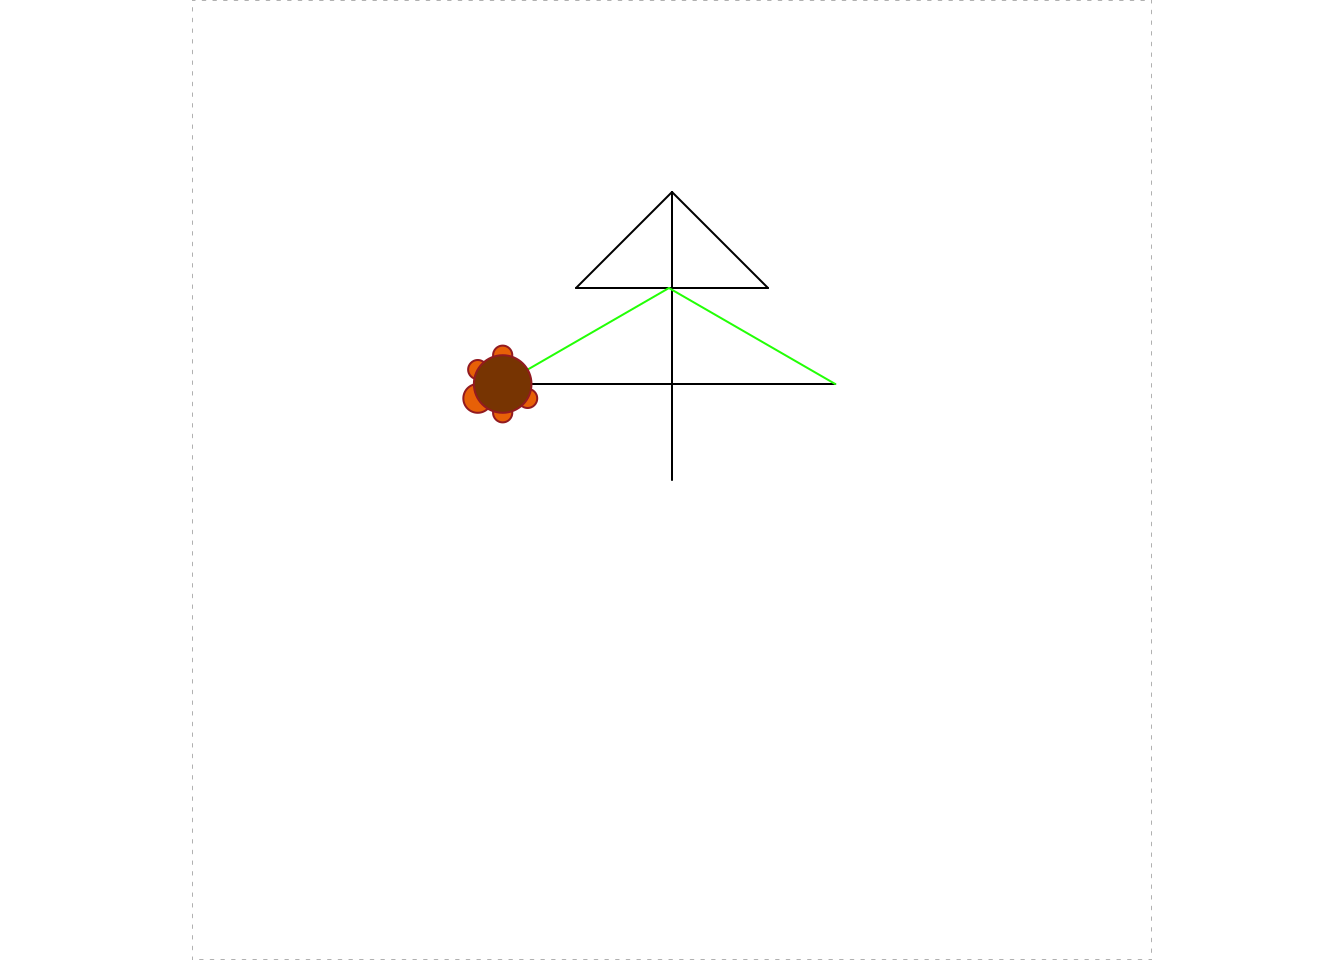
\includegraphics[width=0.5\linewidth]{r-notes_files/figure-latex/hide-show-1} 

}

\caption{The graph after hiding, moving and showing.}\label{fig:hide-show}
\end{figure}

Finally, you can choose the type of line your turtle draws, and the
width of the line. See Figure \ref{fig:type-width} for the results of
the following code.

\begin{Shaded}
\begin{Highlighting}[]
\KeywordTok{turtle_left}\NormalTok{(}\DataTypeTok{angle =} \DecValTok{150}\NormalTok{)}
\KeywordTok{turtle_lty}\NormalTok{(}\DataTypeTok{lty =} \DecValTok{4}\NormalTok{)}
\KeywordTok{turtle_forward}\NormalTok{(}\DataTypeTok{dist =} \DecValTok{17}\NormalTok{)}
\KeywordTok{turtle_lwd}\NormalTok{(}\DataTypeTok{lwd =} \DecValTok{3}\NormalTok{)}
\KeywordTok{turtle_forward}\NormalTok{(}\DataTypeTok{dist =} \DecValTok{15}\NormalTok{)}
\end{Highlighting}
\end{Shaded}

\begin{figure}

{\centering 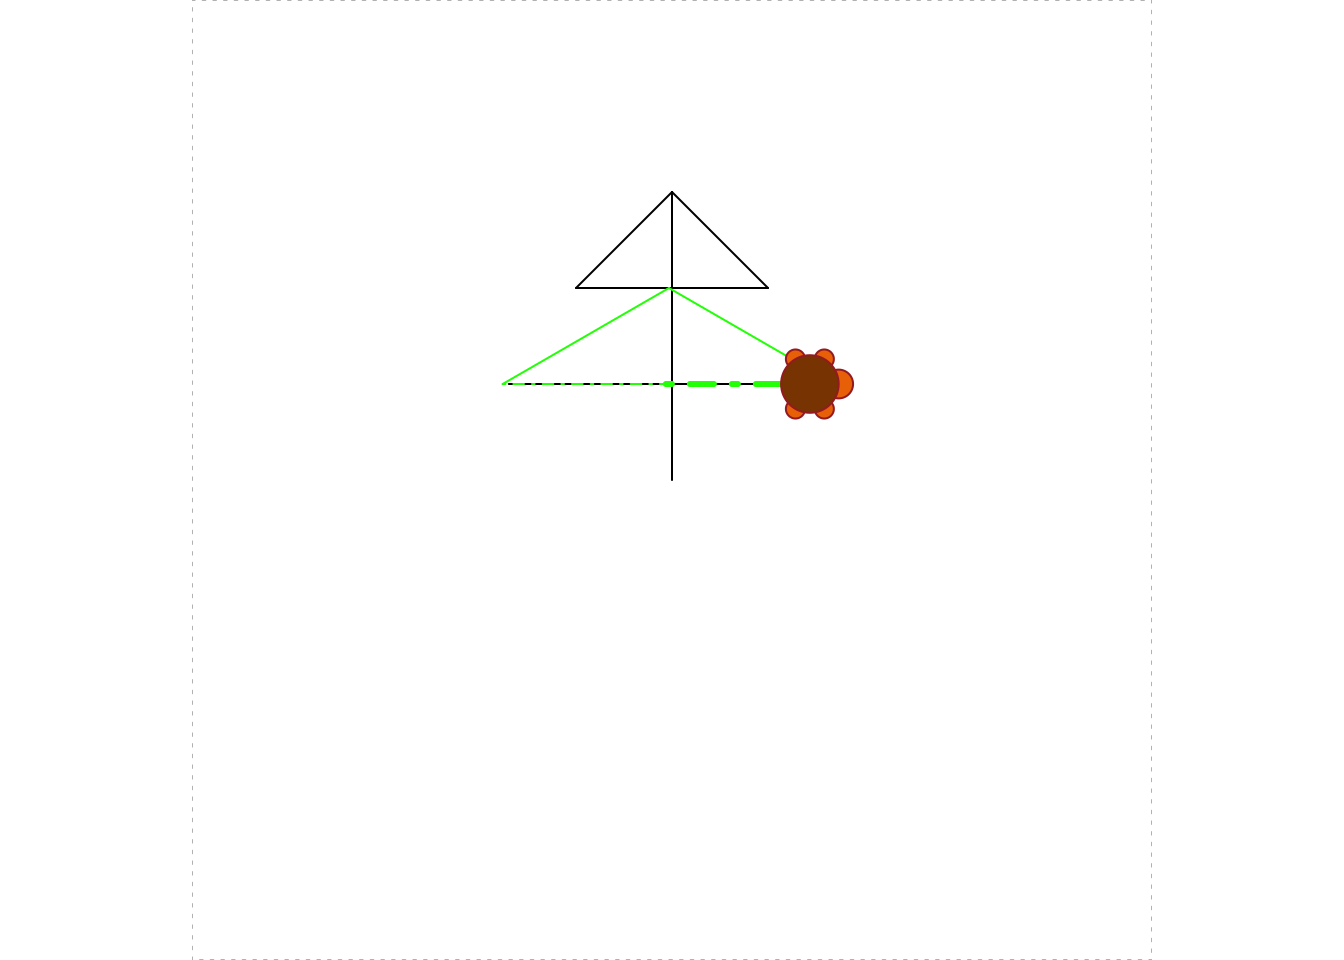
\includegraphics[width=0.5\linewidth]{r-notes_files/figure-latex/type-width-1} 

}

\caption{Choosing line-type and line-width.}\label{fig:type-width}
\end{figure}

\textbf{Note:} you can learn more about \texttt{lty} and \texttt{lwd}
with \texttt{help(par)}.

\section{Making Many Movements: An Introduction to
Looping}\label{making-many-movements-an-introduction-to-looping}

Eventually we want to make some complex figures that require many
movements on the part of the turtle. In order to make these go faster,
we can turn off some of the turtle graphing by wrapping the desired
movements in \texttt{turtle\_do()}. See Figure \ref{fig:turtle-do-intro}
for the results of the following code.

\begin{Shaded}
\begin{Highlighting}[]
\KeywordTok{turtle_init}\NormalTok{()}
\KeywordTok{turtle_do}\NormalTok{(\{}
  \KeywordTok{turtle_move}\NormalTok{(}\DecValTok{10}\NormalTok{)}
  \KeywordTok{turtle_turn}\NormalTok{(}\DecValTok{45}\NormalTok{)}
  \KeywordTok{turtle_move}\NormalTok{(}\DecValTok{15}\NormalTok{)}
\NormalTok{\})}
\end{Highlighting}
\end{Shaded}

\begin{figure}

{\centering 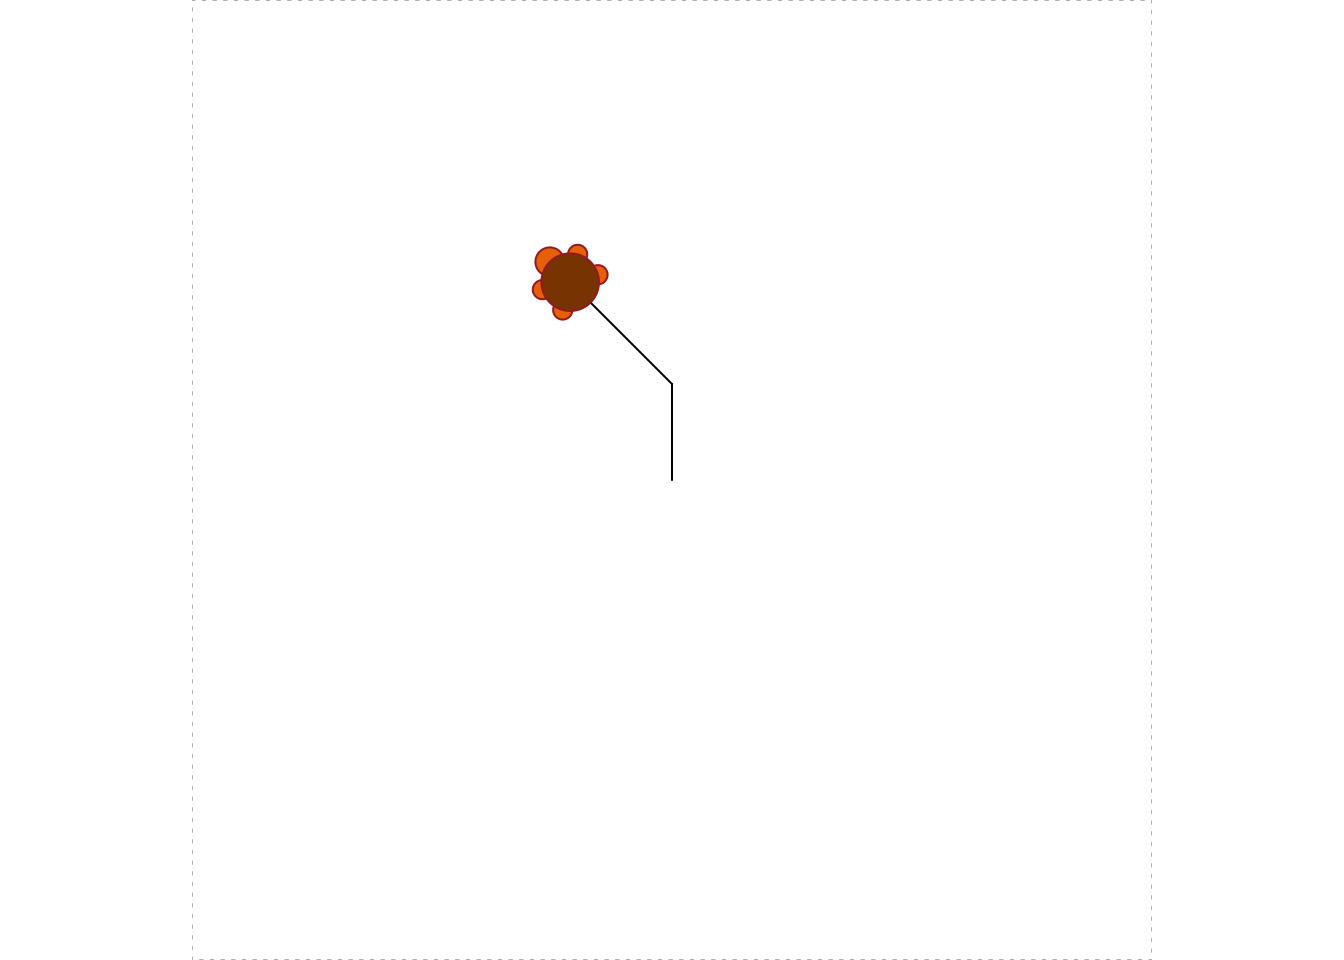
\includegraphics[width=0.5\linewidth]{r-notes_files/figure-latex/turtle-do-intro-1} 

}

\caption{After final movement.}\label{fig:turtle-do-intro}
\end{figure}

(\texttt{turtle\_turn()} turns to the left by default.) Of course, for
such a small number of movements using \texttt{turtle\_do()} does not
matter much, but we will practice using it for a bit.

How might we make a square? The following code offers one way to do it.
See Figure \ref{fig:turtle-square} for the results.

\begin{Shaded}
\begin{Highlighting}[]
\KeywordTok{turtle_init}\NormalTok{()}
\KeywordTok{turtle_do}\NormalTok{(\{}
  \KeywordTok{turtle_move}\NormalTok{(}\DecValTok{20}\NormalTok{)}
  \KeywordTok{turtle_right}\NormalTok{(}\DecValTok{90}\NormalTok{)}
  \KeywordTok{turtle_move}\NormalTok{(}\DecValTok{20}\NormalTok{)}
  \KeywordTok{turtle_right}\NormalTok{(}\DecValTok{90}\NormalTok{)}
  \KeywordTok{turtle_move}\NormalTok{(}\DecValTok{20}\NormalTok{)}
  \KeywordTok{turtle_right}\NormalTok{(}\DecValTok{90}\NormalTok{)}
  \KeywordTok{turtle_move}\NormalTok{(}\DecValTok{20}\NormalTok{)}
  \KeywordTok{turtle_right}\NormalTok{(}\DecValTok{90}\NormalTok{)}
\NormalTok{\})}
\end{Highlighting}
\end{Shaded}

\begin{figure}

{\centering 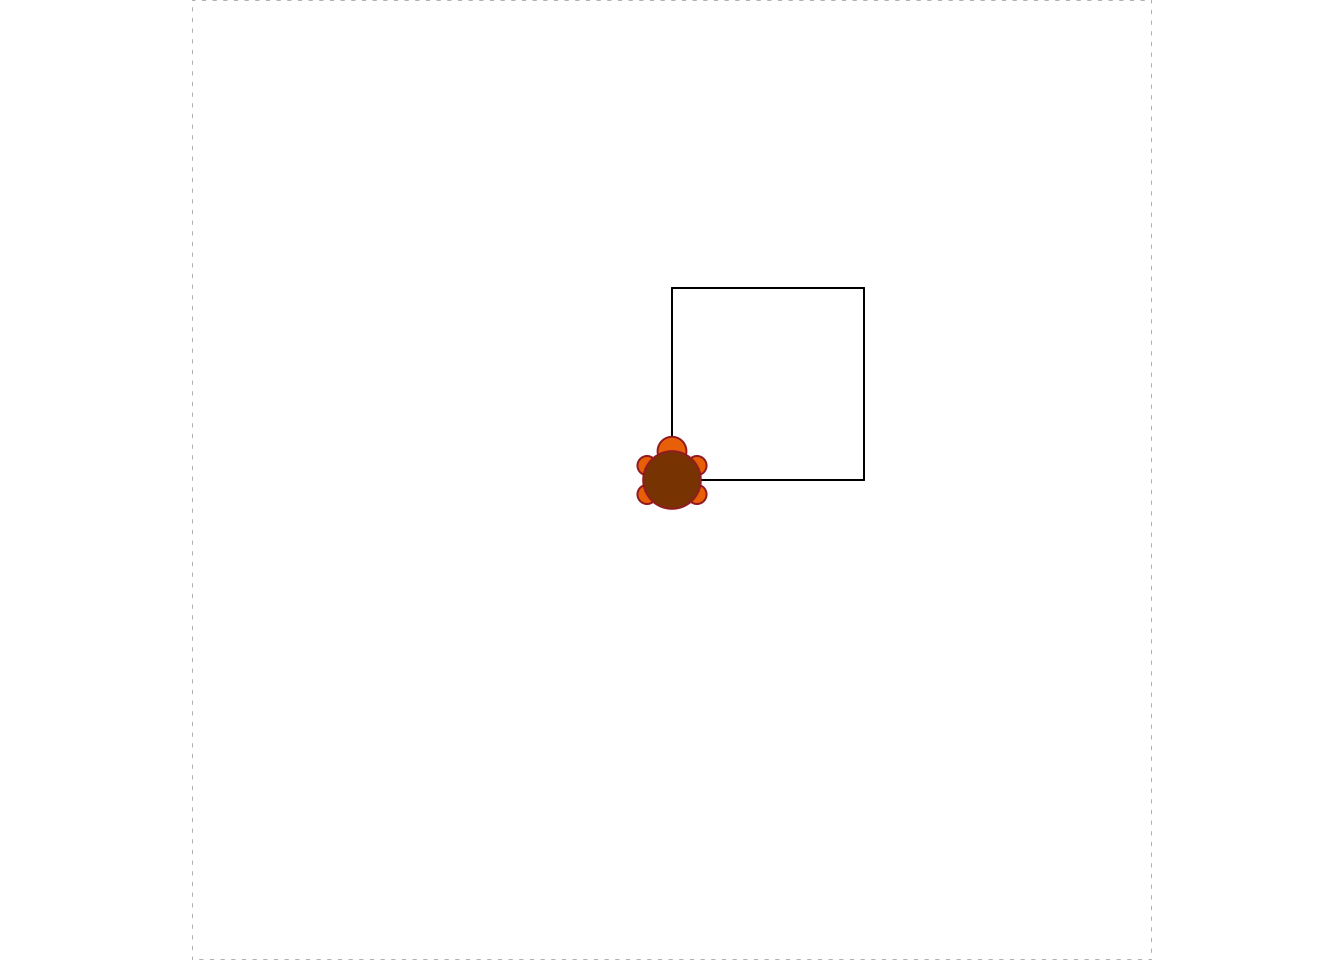
\includegraphics[width=0.5\linewidth]{r-notes_files/figure-latex/turtle-square-1} 

}

\caption{Making a square.}\label{fig:turtle-square}
\end{figure}

This is a bit repetitious. Surely we can take advantage of the fact that
there is a clear pattern to the turtle's movements. A \texttt{for}-loop
seems called for, as in the following code to build the square:

\begin{Shaded}
\begin{Highlighting}[]
\KeywordTok{turtle_init}\NormalTok{()}
\KeywordTok{turtle_do}\NormalTok{(\{}
  \NormalTok{for(i in }\DecValTok{1}\NormalTok{:}\DecValTok{4}\NormalTok{) \{}
    \KeywordTok{turtle_forward}\NormalTok{(}\DataTypeTok{dist =} \DecValTok{20}\NormalTok{)}
    \KeywordTok{turtle_right}\NormalTok{(}\DataTypeTok{angle =} \DecValTok{90}\NormalTok{)}
  \NormalTok{\}}
\NormalTok{\})}
\end{Highlighting}
\end{Shaded}

As we learned in Chapter \ref{flow}, the more you need to repeat a
particular pattern, the more it makes sense to write your code with a
loop. Suppose, for example, that you decide to make regular octagons. A
regular octagon has eight sides, and you turn 45 degrees after drawing
each side. You can do this easily by modifying the square-code as
follows (see Figure \ref{fig:turtle-octagon} for the results):

\begin{Shaded}
\begin{Highlighting}[]
\KeywordTok{turtle_init}\NormalTok{()}
\KeywordTok{turtle_do}\NormalTok{(\{}
  \NormalTok{for(i in }\DecValTok{1}\NormalTok{:}\DecValTok{8}\NormalTok{) \{}
    \KeywordTok{turtle_forward}\NormalTok{(}\DataTypeTok{dist =} \DecValTok{20}\NormalTok{)}
    \KeywordTok{turtle_right}\NormalTok{(}\DataTypeTok{angle =} \DecValTok{45}\NormalTok{)}
  \NormalTok{\}}
\NormalTok{\})}
\end{Highlighting}
\end{Shaded}

\begin{figure}

{\centering 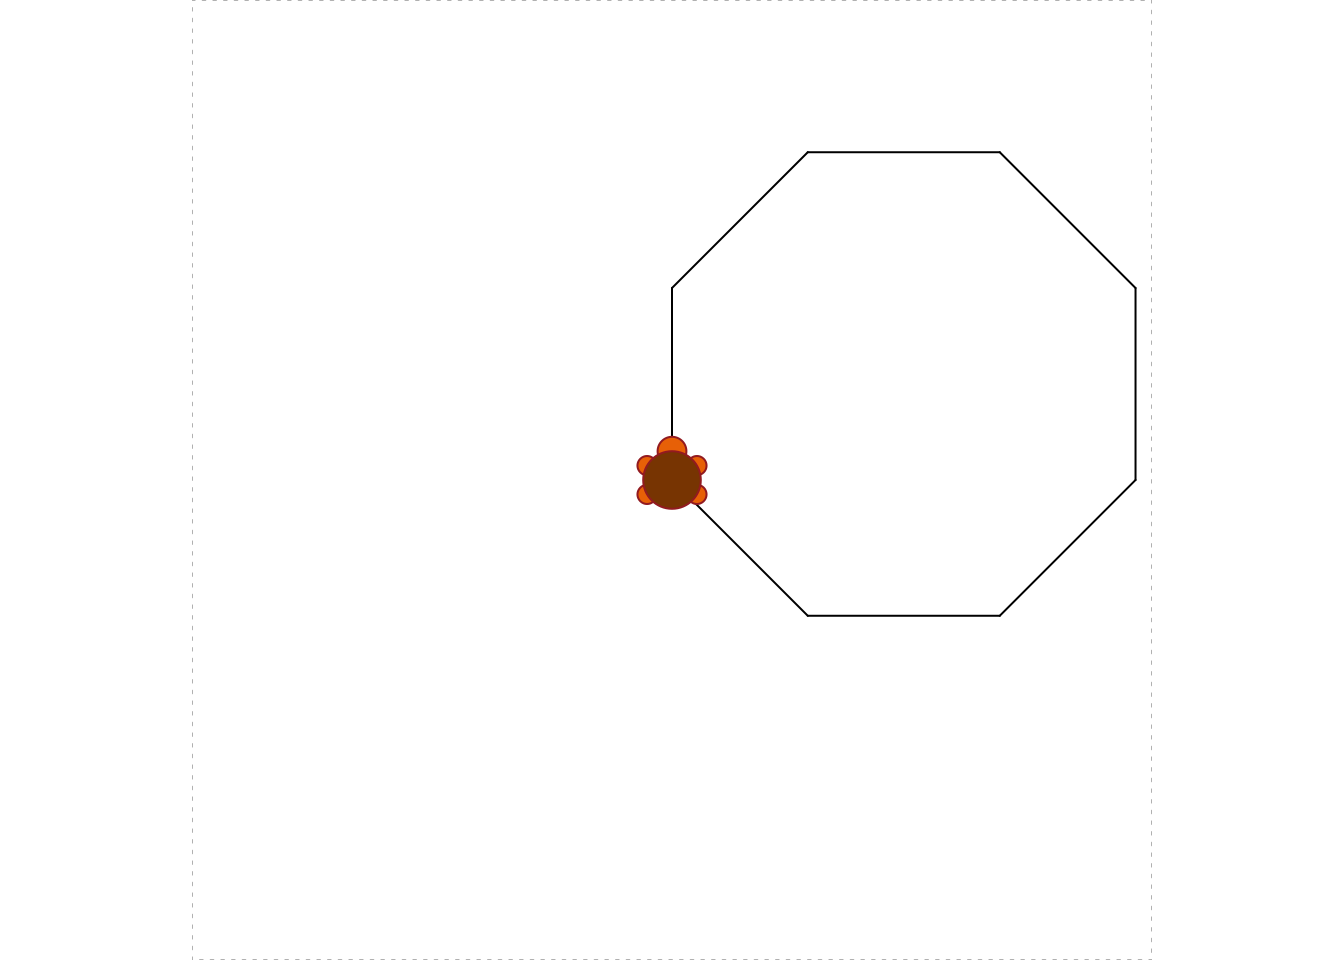
\includegraphics[width=0.5\linewidth]{r-notes_files/figure-latex/turtle-octagon-1} 

}

\caption{Making an octagon.}\label{fig:turtle-octagon}
\end{figure}

You can even make many small turns, so that the resulting figure starts
to look like a circle (see Figure \ref{fig:turtle-circle} for the
results):

\begin{Shaded}
\begin{Highlighting}[]
\KeywordTok{turtle_init}\NormalTok{()}
\KeywordTok{turtle_setpos}\NormalTok{(}\DataTypeTok{x =} \DecValTok{30}\NormalTok{, }\DataTypeTok{y =} \DecValTok{50}\NormalTok{)}
\KeywordTok{turtle_do}\NormalTok{(\{}
  \NormalTok{for(i in }\DecValTok{1}\NormalTok{:}\DecValTok{180}\NormalTok{) \{}
    \KeywordTok{turtle_forward}\NormalTok{(}\DataTypeTok{dist =} \DecValTok{1}\NormalTok{)}
    \KeywordTok{turtle_right}\NormalTok{(}\DataTypeTok{angle =} \DecValTok{2}\NormalTok{)}
  \NormalTok{\}}
\NormalTok{\})}
\end{Highlighting}
\end{Shaded}

\begin{figure}

{\centering 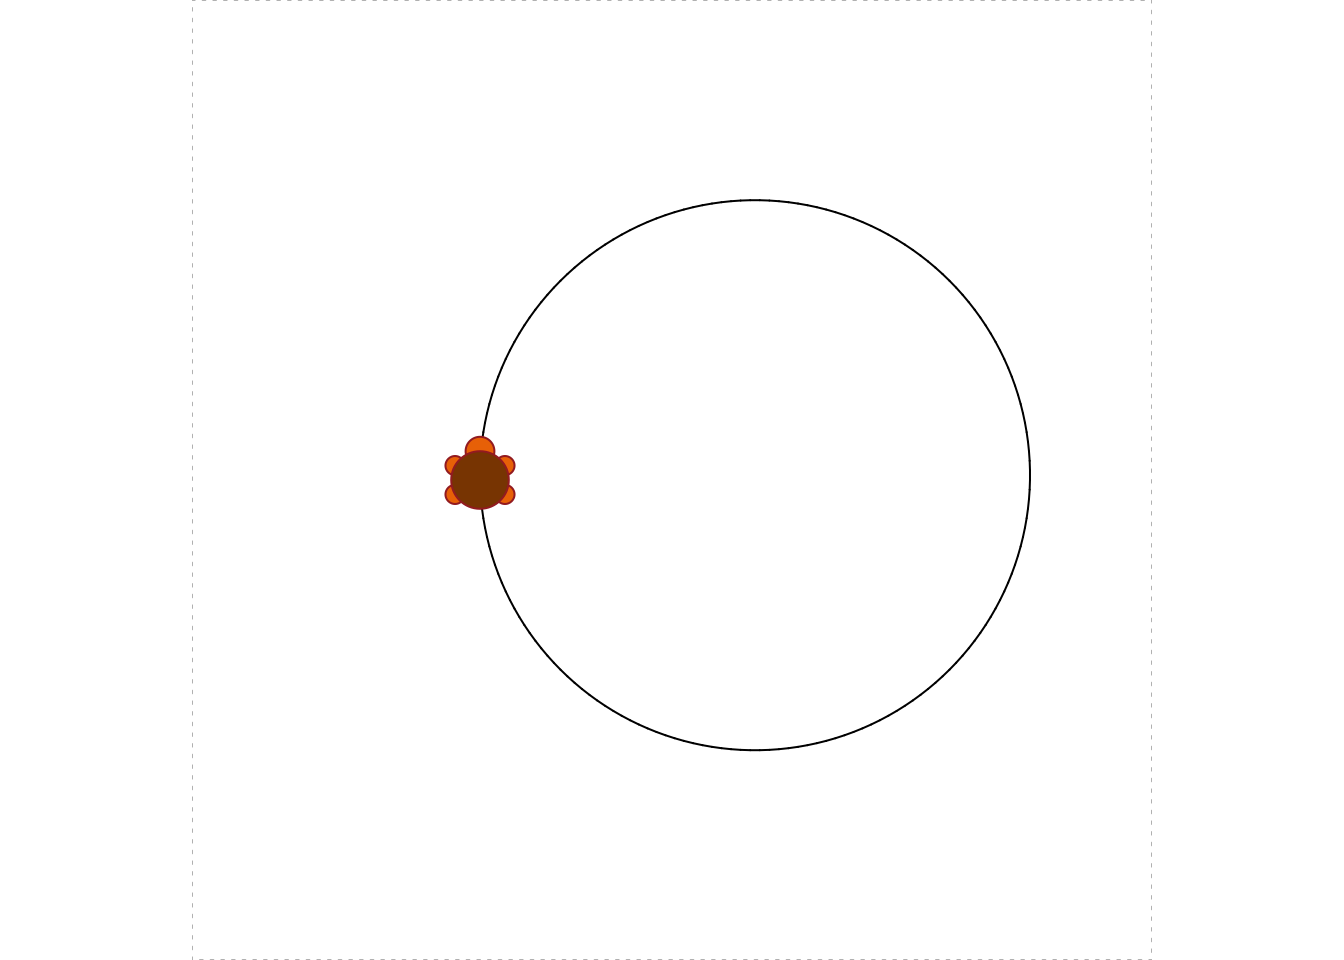
\includegraphics[width=0.5\linewidth]{r-notes_files/figure-latex/turtle-circle-1} 

}

\caption{Making a circle.}\label{fig:turtle-circle}
\end{figure}

Notice that in the above code the turtle was initially set a bit to the
left of center, so that the resulting circle would be situated close to
middle of the region.

If you allow the index variable to be involved in the computations in
the body of the loop then you can start making more complex figures. For
example, here is the code for a spiral (see Figure
\ref{fig:turtle-spiral} for the results):

\begin{Shaded}
\begin{Highlighting}[]
\KeywordTok{turtle_init}\NormalTok{(}\DataTypeTok{width =} \DecValTok{150}\NormalTok{, }\DataTypeTok{height =} \DecValTok{150}\NormalTok{, }\DataTypeTok{mode =} \StringTok{"clip"}\NormalTok{)}
\KeywordTok{turtle_do}\NormalTok{(\{}
  \KeywordTok{turtle_right}\NormalTok{(}\DecValTok{90}\NormalTok{)}
  \NormalTok{for (i in }\DecValTok{1}\NormalTok{:}\DecValTok{720}\NormalTok{) \{}
    \KeywordTok{turtle_left}\NormalTok{(}\DecValTok{1}\NormalTok{)}
    \KeywordTok{turtle_forward}\NormalTok{(i/}\DecValTok{720}\NormalTok{)}
  \NormalTok{\}}
\NormalTok{\})}
\end{Highlighting}
\end{Shaded}

\begin{figure}

{\centering 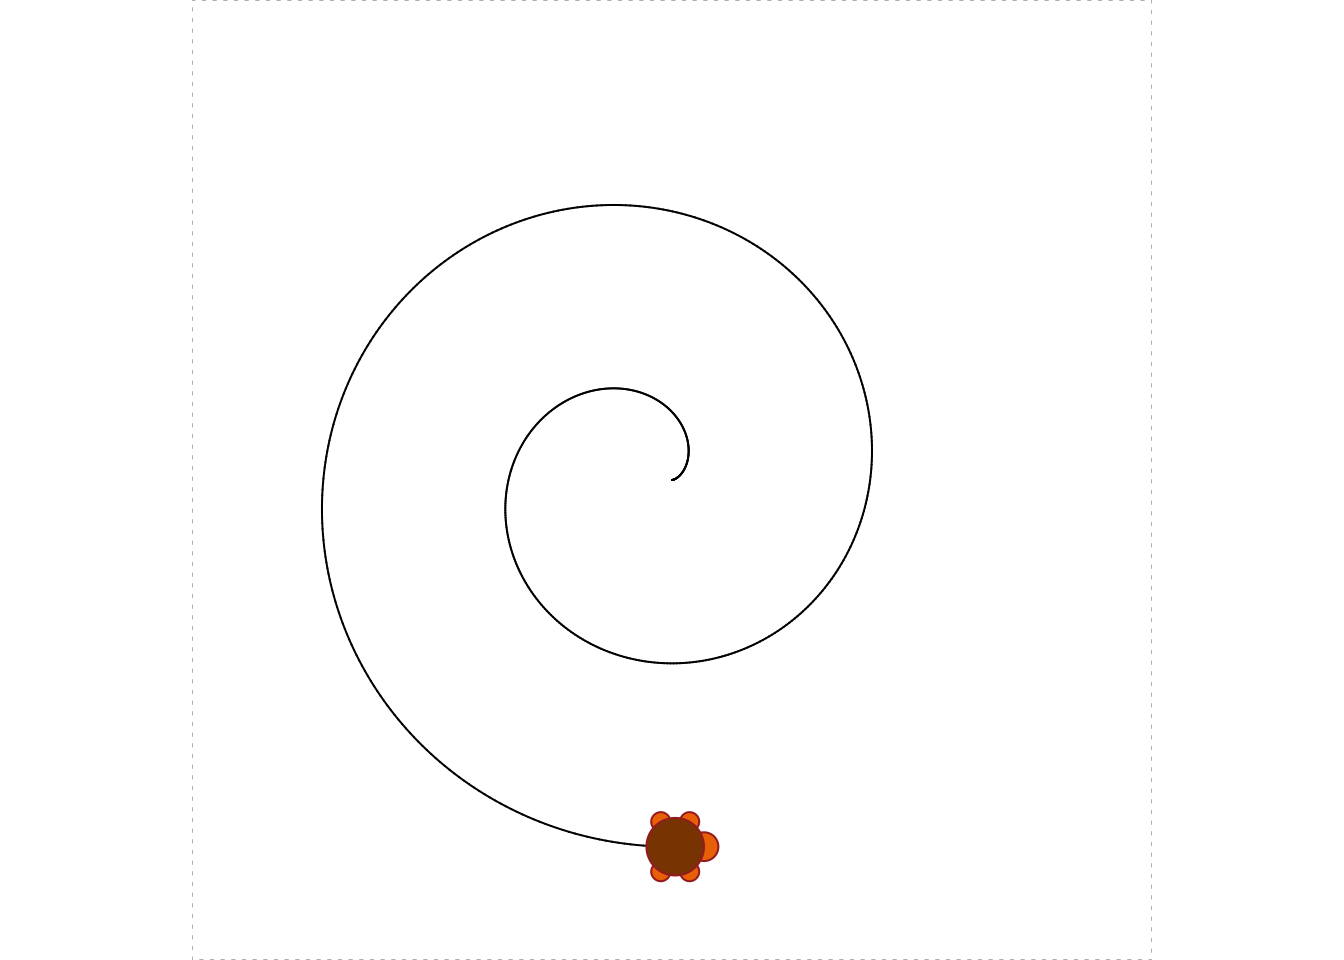
\includegraphics[width=0.5\linewidth]{r-notes_files/figure-latex/turtle-spiral-1} 

}

\caption{Using a loop to make a spiral.}\label{fig:turtle-spiral}
\end{figure}

The turtle turns one degree every time R goes through the loop, but the
amount it travels forward (\(i/720\)) increases as the index variable
\texttt{i} increases.\footnote{Another thing to notice is that we set
  the width and height of the region ourselves, so that the spiral would
  fit into it. We also set \texttt{mode} to \texttt{clip} rather then
  leaving it at its default value of \texttt{error}. With
  \texttt{mode\ =\ "clip"}, R won't throw an error message at you when
  the turtle moves outside of its region. Clip-mode is very handy when
  you are developing a graph and don't know in advance precisely where
  the turtle will go.}

\section{Writing Turtle Functions}\label{writing-turtle-functions}

Once you have designed some shapes that you think you might want to draw
again, you should write them up as functions. Here for example, is the
code for a function that makes squares:

\begin{Shaded}
\begin{Highlighting}[]
\NormalTok{turtle_square <-}\StringTok{ }\NormalTok{function(side) \{ }
  \NormalTok{for (i in }\DecValTok{1}\NormalTok{:}\DecValTok{4}\NormalTok{) \{}
    \KeywordTok{turtle_forward}\NormalTok{(side)}
    \KeywordTok{turtle_right}\NormalTok{(}\DecValTok{90}\NormalTok{) }
  \NormalTok{\}}
\NormalTok{\}}
\end{Highlighting}
\end{Shaded}

Note that the user can vary the length of a side.

Functions are nice, but note that \texttt{turtle\_do()} cannot be used
freely inside of them. For example, suppose you were to write the
square-making function as follows:

\begin{Shaded}
\begin{Highlighting}[]
\NormalTok{turtle_square <-}\StringTok{ }\NormalTok{function(side) \{ }
  \KeywordTok{turtle_do}\NormalTok{(\{}
    \NormalTok{for (i in }\DecValTok{1}\NormalTok{:}\DecValTok{4}\NormalTok{) \{}
      \KeywordTok{turtle_forward}\NormalTok{(side)}
      \KeywordTok{turtle_right}\NormalTok{(}\DecValTok{90}\NormalTok{)}
    \NormalTok{\}}
  \NormalTok{\})}
\NormalTok{\}}
\end{Highlighting}
\end{Shaded}

Attempting to use the function would result in an error:

\begin{Shaded}
\begin{Highlighting}[]
\KeywordTok{turtle_init}\NormalTok{()}
\KeywordTok{turtle_square}\NormalTok{(}\DecValTok{50}\NormalTok{)}
\end{Highlighting}
\end{Shaded}

\begin{verbatim}
 Error in stopifnot(is.numeric(distance), 
   length(distance) == 1, is.finite(distance)) : 
  object 'side' not found 
\end{verbatim}

\texttt{turtle\_do()} cannot find the side-length argument that was
passed into the function. Although \texttt{turtle\_do()} can appear
inside of functions, it has to work on literal values, not on variables.

\section{Random Moves}\label{random-moves}

So far our turtle has moved in very regular and disciplined ways. It's
time to break the pattern, a bit. R has a quite a few functions to
generate numbers that look ``random''; we will use some of these
functions to make the turtle move about randomly.

\subsection{Sampling from a Vector}\label{sampling-from-a-vector}

You have already met the \texttt{sample()}
\index{R-functions!sample()@\texttt{sample()}}function (see Section
\ref{if-statements}). Let's take a closer look at it.

\texttt{sample()} makes a random choice from a given vector. From the
R-help we read that the general form of a call to sample is as follows:

\begin{Shaded}
\begin{Highlighting}[]
\KeywordTok{sample}\NormalTok{(x, size, }\DataTypeTok{replace =} \OtherTok{FALSE}\NormalTok{, }\DataTypeTok{prob =} \OtherTok{NULL}\NormalTok{)}
\end{Highlighting}
\end{Shaded}

In the above call:

\begin{itemize}
\tightlist
\item
  \texttt{x} is the vector from which we wish to sample (R refers to it
  as the ``population'');
\item
  \texttt{size} is the number of random samples we want;
\item
  \texttt{replace} says whether or not to replace each member of the
  population after we have sampled it.
\item
  \texttt{prob} specifies the desired probability for each member of the
  population to be chosen.
\end{itemize}

A few examples will help us understand how the arguments work:

\begin{Shaded}
\begin{Highlighting}[]
\NormalTok{vec <-}\StringTok{ }\DecValTok{1}\NormalTok{:}\DecValTok{10} \CommentTok{# we'll sample from this vector}
\KeywordTok{sample}\NormalTok{(vec, }\DecValTok{1}\NormalTok{)}
\end{Highlighting}
\end{Shaded}

\begin{verbatim}
## [1] 7
\end{verbatim}

We got only one number because we set \texttt{size} to 1. Every element
in \texttt{vec} had an equal chance of being the element selected. This
time we got 7, but if you were to run the function again for yourself
your results would probably be different.

Let's sample 10 numbers from \texttt{vec}:

\begin{Shaded}
\begin{Highlighting}[]
\KeywordTok{sample}\NormalTok{(vec, }\DecValTok{10}\NormalTok{)}
\end{Highlighting}
\end{Shaded}

\begin{verbatim}
##  [1]  3  5  2  4  7  6  9  1  8 10
\end{verbatim}

Because \texttt{replace} was left at its default value of
\texttt{FALSE}, R did not replace numbers after pulling them from the
\texttt{vec}. After each sample, the remaining numbers all had the same
chance to be picked next. Setting \texttt{size} to the length of
\texttt{x} and keeping \texttt{replace\ =\ FALSE} therefore has the
effect of randomly shuffling the elements of \texttt{x}.

Of course when \texttt{replace\ =\ FALSE} any attempt to sample more
than the number of elements of \texttt{vec} will result in an error:

\begin{Shaded}
\begin{Highlighting}[]
\KeywordTok{sample}\NormalTok{(vec, }\DecValTok{11}\NormalTok{)}
\end{Highlighting}
\end{Shaded}

\begin{verbatim}
Error in sample.int(length(x), size, replace, prob) : 
cannot take a sample larger than the 
population when 'replace = FALSE'
\end{verbatim}

When we set \texttt{replace\ =\ TRUE} then each selected element is
returned to the population. At any stage, the chance for a given member
of the population to be the one selected next is the same---no matter
how many times that member has already been selected. Thus, when
\texttt{replace\ =\ TRUE} you are liable to see repeats:

\begin{Shaded}
\begin{Highlighting}[]
\KeywordTok{sample}\NormalTok{(vec, }\DecValTok{20}\NormalTok{, }\DataTypeTok{replace =} \NormalTok{T)}
\end{Highlighting}
\end{Shaded}

\begin{verbatim}
##  [1]  3  8  8  8  8  9  5  6  7  1  4  8  4  1 10  6  3  3  1  9
\end{verbatim}

When the \texttt{prob} parameter is left at its \texttt{NULL} value, R
gives each member of the population the \emph{same} chance to be the
member that is selected. It is possible to adjust the probabilities of
selection by setting \texttt{prob} to a vector of probabilities (one for
each corresponding member of \texttt{x}). Thus, suppose we want to
select 20 numbers from \texttt{vec}, according to the following the
probabilities:

\begin{itemize}
\tightlist
\item
  5\% chance of selection, for each number from 1 to 8;
\item
  30\% chance for 9 to be selected;
\item
  30\% chance for 10 to be selected.
\end{itemize}

Then we can call \texttt{sample()} like this:

\begin{Shaded}
\begin{Highlighting}[]
\KeywordTok{sample}\NormalTok{(vec, }\DecValTok{20}\NormalTok{, }\DataTypeTok{replace =} \NormalTok{T,}
       \DataTypeTok{prob  =} \KeywordTok{c}\NormalTok{(}\KeywordTok{rep}\NormalTok{(}\FloatTok{0.05}\NormalTok{, }\DecValTok{8}\NormalTok{), }\FloatTok{0.30}\NormalTok{, }\FloatTok{0.30}\NormalTok{))}
\end{Highlighting}
\end{Shaded}

\begin{verbatim}
##  [1]  9  1  9 10  9  6  8  9  4  7 10 10  9  2  6  9  5  9 10 10
\end{verbatim}

Notice that we a majority of 9's and 10's: this was fairly likely to
occur since each selection had a 60\% chance of turning out to be 9 or
10.

\subsection{Application: a Bouncing
Turtle}\label{application-a-bouncing-turtle}

Let's apply \texttt{sample()} to design a scenario in which the turtle
moves a fixed amount at each step, but the direction---north, east,
south, or west---is completely random. When the turtle reaches the
boundary of its domain, however, we would like it to ``bounce back'':
i.e., take a step in the direction opposite to the step that brought it
to the boundary. We will also query the user prior to each step, asking
if he/she wants to see another move. This not only allows the user to
decide when to end the scenario; it also permits the user to see where
the turtle is after each step.

One possible implementation is as follows:

\begin{Shaded}
\begin{Highlighting}[]
\NormalTok{turtle_bounce <-}\StringTok{ }\NormalTok{function(}\DataTypeTok{side =} \DecValTok{60}\NormalTok{, }\DataTypeTok{step=} \DecValTok{10}\NormalTok{) \{}
  \NormalTok{if ( (side/}\DecValTok{2}\NormalTok{) %%}\StringTok{ }\NormalTok{step !=}\StringTok{ }\DecValTok{0} \NormalTok{) \{}
    \KeywordTok{stop}\NormalTok{(}\StringTok{"Side-length divided by two must be a multiple of step."}\NormalTok{)}
  \NormalTok{\}}
  \NormalTok{bounds <-}\StringTok{ }\KeywordTok{c}\NormalTok{(}\DecValTok{0}\NormalTok{, side)}
  \KeywordTok{turtle_init}\NormalTok{(side, side, }\DataTypeTok{mode =} \StringTok{"clip"}\NormalTok{)}
  \NormalTok{origin <-}\StringTok{ }\KeywordTok{turtle_getpos}\NormalTok{()}
  \NormalTok{cp <-}\StringTok{ }\KeywordTok{turtle_getpos}\NormalTok{()}
  \NormalTok{repeat \{}
    \NormalTok{move <-}\StringTok{ }\KeywordTok{readline}\NormalTok{(}\DataTypeTok{prompt =} \StringTok{"Go Again? (enter q to quit):  "}\NormalTok{)}
    \NormalTok{if ( move ==}\StringTok{ "q"}\NormalTok{) break}
    \NormalTok{x <-}\StringTok{ }\NormalTok{cp[}\StringTok{"x"}\NormalTok{]}
    \NormalTok{y <-}\StringTok{ }\NormalTok{cp[}\StringTok{"y"}\NormalTok{]}
    \NormalTok{if (x %in%}\StringTok{ }\NormalTok{bounds |}\StringTok{ }\NormalTok{y %in%}\StringTok{ }\NormalTok{bounds) \{}
      \NormalTok{angle <-}\StringTok{ }\DecValTok{180}
    \NormalTok{\} else \{}
      \NormalTok{angle <-}\StringTok{ }\KeywordTok{sample}\NormalTok{(}\KeywordTok{c}\NormalTok{(}\DecValTok{0}\NormalTok{,}\DecValTok{90}\NormalTok{,}\DecValTok{180}\NormalTok{,}\DecValTok{270}\NormalTok{), }\DecValTok{1}\NormalTok{)}
    \NormalTok{\}}
    \KeywordTok{turtle_right}\NormalTok{(angle)}
    \KeywordTok{turtle_forward}\NormalTok{(step)}
    \NormalTok{cp <-}\StringTok{ }\KeywordTok{round}\NormalTok{(}\KeywordTok{turtle_getpos}\NormalTok{(), }\DecValTok{0}\NormalTok{)}
    \KeywordTok{print}\NormalTok{(cp)}
  \NormalTok{\}}
  \KeywordTok{cat}\NormalTok{(}\StringTok{"All done!"}\NormalTok{)}
\NormalTok{\}}
\end{Highlighting}
\end{Shaded}

Play the game a few times, to get a feel for how it works:

\begin{Shaded}
\begin{Highlighting}[]
\KeywordTok{turtle_bounce}\NormalTok{(}\DecValTok{60}\NormalTok{, }\DecValTok{15}\NormalTok{)}
\end{Highlighting}
\end{Shaded}

Let's examine the code a bit more closely.

The definition indicates that there are two parameters: \texttt{side}
and \texttt{step}.

\begin{itemize}
\tightlist
\item
  The \texttt{side} parameter gives the dimensions of the Turtle's
  field. Thus if \texttt{side} were set to 60---which is the
  default---then the field would be a 60-by-60 square, with the origin
  \((0,0)\) in at lower-left corner and the point \((60, 60)\) at the
  upper-right corner. When the turtle is initialized it will appear in
  the middle of the square, at the point \((30, 30)\).
\item
  \texttt{step} specifies how many units the turtle will move at each
  step. In this analysis we will assume that \texttt{step} is set to 15.
\end{itemize}

Inside the function, we begin with a bit of input-validation:

\begin{Shaded}
\begin{Highlighting}[]
\NormalTok{if ( (side/}\DecValTok{2}\NormalTok{) %%}\StringTok{ }\NormalTok{step !=}\StringTok{ }\DecValTok{0} \NormalTok{) \{}
    \KeywordTok{stop}\NormalTok{(}\StringTok{"Side-length divided by two must be a multiple of step."}\NormalTok{)}
  \NormalTok{\}}
\end{Highlighting}
\end{Shaded}

Remember that the turtle will start at
\((\texttt{side}/2, \texttt{side}/2)\) and will move \texttt{step} each
time. If \(\texttt{side}/2\) is not evenly divisible by \texttt{step}
then the turtle would be able to go from inside its field to outside in
a single step. We don't want that to happen so we stop the user if the
remainder after dividing \(\texttt{side}/2\) by \texttt{side} is
anything other than zero.

If the input is OK, then we set up a vector \texttt{bounds} that records
the smallest and largest possible values for the \(x\) and \(y\)
coordinates of the turtle:

\begin{Shaded}
\begin{Highlighting}[]
\NormalTok{bounds <-}\StringTok{ }\KeywordTok{c}\NormalTok{(}\DecValTok{0}\NormalTok{, side)}
\end{Highlighting}
\end{Shaded}

Next, we initialize the turtle in the middle of the field and record its
initial position in the vector \texttt{cp}:

\begin{Shaded}
\begin{Highlighting}[]
\KeywordTok{turtle_init}\NormalTok{(side, side, }\DataTypeTok{mode =} \StringTok{"clip"}\NormalTok{)}
\NormalTok{origin <-}\StringTok{ }\KeywordTok{turtle_getpos}\NormalTok{()}
\NormalTok{cp <-}\StringTok{ }\KeywordTok{turtle_getpos}\NormalTok{()}
\end{Highlighting}
\end{Shaded}

(You can think of \texttt{cp} as short for: ``current position''.)

Next, we enter a \texttt{repeat}-loop. Inside the loop we begin with:

\begin{Shaded}
\begin{Highlighting}[]
\NormalTok{move <-}\StringTok{ }\KeywordTok{readline}\NormalTok{(}\DataTypeTok{prompt =} \StringTok{"Go Again? (enter q to quit):  "}\NormalTok{)}
\NormalTok{if ( move ==}\StringTok{ "q"}\NormalTok{) break}
\NormalTok{x <-}\StringTok{ }\NormalTok{cp[}\StringTok{"x"}\NormalTok{]}
\NormalTok{y <-}\StringTok{ }\NormalTok{cp[}\StringTok{"y"}\NormalTok{]}
\end{Highlighting}
\end{Shaded}

We first asked the user if she wanted to quit. If she enters ``q'' then
we'll break out of the loop and end the scenario. If she enters anything
else (including just pressing Enter) then we record the \(x\) and \(y\)
coordinates of the turtle's current position in the vectors \texttt{x}
and \texttt{y} respectively.

Our next task is to determine how the turtle should move:

\begin{Shaded}
\begin{Highlighting}[]
\NormalTok{if (x %in%}\StringTok{ }\NormalTok{bounds |}\StringTok{ }\NormalTok{y %in%}\StringTok{ }\NormalTok{bounds) \{}
      \NormalTok{angle <-}\StringTok{ }\DecValTok{180}
    \NormalTok{\} else \{}
      \NormalTok{angle <-}\StringTok{ }\KeywordTok{sample}\NormalTok{(}\KeywordTok{c}\NormalTok{(}\DecValTok{0}\NormalTok{,}\DecValTok{90}\NormalTok{,}\DecValTok{180}\NormalTok{,}\DecValTok{270}\NormalTok{), }\DecValTok{1}\NormalTok{)}
    \NormalTok{\}}
\end{Highlighting}
\end{Shaded}

If the turtle is at a boundary (either \texttt{x} equal to 0 or 60 or
\texttt{y} equal to 0 or 60) then we need to ``bounce back''. This
corresponds to making the turtle turn right by 180 degrees and then
step. On the other hand if the turtle is not at a boundary then the
direction of the turtle should be random, so we should have it turn
right by either 0, 90, 180 or 270 degrees, with each possibility being
equally likely. This is accomplished with the above call to the
\texttt{sample()} function.

Having determined the amount by which to turn prior to the next step, we
then have the turtle turn that amount and take the step:

\begin{Shaded}
\begin{Highlighting}[]
\KeywordTok{turtle_right}\NormalTok{(angle)}
\KeywordTok{turtle_forward}\NormalTok{(step)}
\end{Highlighting}
\end{Shaded}

Finally, we set \texttt{cp} to the new position of the turtle, and print
that position out to the console for the user to see:

\begin{Shaded}
\begin{Highlighting}[]
\NormalTok{cp <-}\StringTok{ }\KeywordTok{round}\NormalTok{(}\KeywordTok{turtle_getpos}\NormalTok{(), }\DecValTok{0}\NormalTok{)}
\KeywordTok{print}\NormalTok{(cp)}
\end{Highlighting}
\end{Shaded}

Note that we rounded off the position to the nearest while number. This
was done because the authors of the \textbf{TurtleGraphics} package use
floating point arithmetic for their numerical operations, so sometimes
the computed positions differ from whole numbers by a very tiny amount.

We then repeat the loop.

\subsection{Uniform Random Numbers}\label{uniform-random-numbers}

\texttt{sample()} picks an element from a finite population. Sometimes,
though, we want R to give the impression that it has picked a \emph{real
number} at random out of a range of real numbers. This can be
accomplished with the \texttt{runif()}
function.\index{R-functions!runif()@\texttt{runif()}}

A call to \texttt{runif()} looks like this:

\begin{Shaded}
\begin{Highlighting}[]
\KeywordTok{runif}\NormalTok{(n, }\DataTypeTok{min =} \DecValTok{0}\NormalTok{, }\DataTypeTok{max =} \DecValTok{1}\NormalTok{)}
\end{Highlighting}
\end{Shaded}

The idea is that R will produce \texttt{n} real numbers that have the
appearance of having been drawn randomly from the interval of real
numbers whose lower and upper bounds are specified respectively by
\texttt{min} and \texttt{max}.

Thus, to get 10 ``random'' numbers that all lie between 0 and 1, you can
leave \texttt{min} and \texttt{max} at their defaults and ask for:

\begin{Shaded}
\begin{Highlighting}[]
\KeywordTok{runif}\NormalTok{(}\DecValTok{10}\NormalTok{)}
\end{Highlighting}
\end{Shaded}

\begin{verbatim}
##  [1] 0.646902839 0.394225758 0.618501814 0.476891136 0.136097186
##  [6] 0.067384386 0.129152617 0.393117930 0.002582699 0.620205954
\end{verbatim}

\subsection{Pseudo-Randomness and Setting a
Seed}\label{pseudo-randomness-and-setting-a-seed}

It's important to point out that R doesn't generate truly random
numbers.\footnote{Indeed, philosophers of mathematics debate what
  randomness ``really'' is.} After all, R simply runs a computer which
operates according to a set of completely-specified steps. Thus the
random data generated by R and by other computer languages is often
called \emph{pseudorandom}. \index{pseudo-random numbers}Although the
functions for random-number generation have been carefully designed so
as to follow many of the statistical laws we associate with randomness
in nature, all of the pseudo-random output is determined by an initial
value and a deterministic number-generating algorithm.

We actually have the ability to set the pseudorandom data ourselves.
This is called \emph{setting the random seed}. From any specified seed,
the result of calls to R's random-data functions will be completely
determined (although---just as in the case of ``real'' randomness---the
output will still probably ``look'' random).

The \texttt{set.seed()}
function\index{R-functions!set.seed()@\texttt{set.seed()}} will fix the
random output. Try running the following two lines of code more than
once:

\begin{Shaded}
\begin{Highlighting}[]
\KeywordTok{set.seed}\NormalTok{(}\DecValTok{2025}\NormalTok{)}
\KeywordTok{runif}\NormalTok{(}\DecValTok{10}\NormalTok{)}
\end{Highlighting}
\end{Shaded}

\begin{verbatim}
##  [1] 0.7326202 0.4757614 0.5142159 0.4984323 0.7802845 0.5042522 0.8984003
##  [8] 0.1278527 0.6446721 0.5695311
\end{verbatim}

You will get the same output every time. If you change the argument of
\texttt{set.seed()} to some other integer the output will probably
change---but it will stay the same when you run the code \emph{again}
from that that new seed.

\subsection{Application: a Drunken Turtle}\label{drunken-turtle-intro}

We will now modify the previous scenario so that the turtle's motion
will be almost completely random. Even though it will take the same-size
step every time, the angle at which it steps will be completely random:
any real number of degrees from 0 to 360. We will also show the user the
position of the turtle at each step, and use the ``distance formula''
from high-school geometry to compute and display the current distance of
the turtle from the place where it started.

\begin{Shaded}
\begin{Highlighting}[]
\NormalTok{turtle_drunk <-}\StringTok{ }\NormalTok{function(side, step) \{}
  \KeywordTok{turtle_init}\NormalTok{(side, side, }\DataTypeTok{mode =} \StringTok{"clip"}\NormalTok{)}
  \CommentTok{# save (side/2, side/2), the turtle's initial position:}
  \NormalTok{initial <-}\StringTok{ }\KeywordTok{turtle_getpos}\NormalTok{()}
  \NormalTok{repeat \{}
    \NormalTok{move <-}\StringTok{ }\KeywordTok{readline}\NormalTok{(}\DataTypeTok{prompt =} \StringTok{"Go Again? (enter q to quit):  "}\NormalTok{)}
    \NormalTok{if ( move ==}\StringTok{ "q"}\NormalTok{) break}
    \CommentTok{# pick a random angle to turn by:}
    \NormalTok{angle <-}\StringTok{ }\KeywordTok{runif}\NormalTok{(}\DecValTok{1}\NormalTok{, }\DataTypeTok{min =} \DecValTok{0}\NormalTok{, }\DataTypeTok{max =} \DecValTok{360}\NormalTok{)}
    \KeywordTok{turtle_left}\NormalTok{(angle)}
    \KeywordTok{turtle_forward}\NormalTok{(step)}
    \CommentTok{# get new position, make it the current position:}
    \NormalTok{cp <-}\StringTok{ }\KeywordTok{turtle_getpos}\NormalTok{()}
    \CommentTok{# print to console:}
    \KeywordTok{print}\NormalTok{(cp)}
    \CommentTok{# determine distnce from initial position (round to 3 decimals):}
    \NormalTok{distance <-}\StringTok{ }\KeywordTok{round}\NormalTok{(}\KeywordTok{sqrt}\NormalTok{((cp[}\DecValTok{1}\NormalTok{] -}\StringTok{ }\NormalTok{initial[}\DecValTok{1}\NormalTok{])^}\DecValTok{2} \NormalTok{+}\StringTok{ }\NormalTok{(cp[}\DecValTok{2}\NormalTok{] -}\StringTok{ }\NormalTok{initial[}\DecValTok{2}\NormalTok{])^}\DecValTok{2}\NormalTok{),}\DecValTok{3}\NormalTok{)}
    \CommentTok{# prepare message to console,and print it:}
    \NormalTok{message <-}\StringTok{ }\KeywordTok{paste0}\NormalTok{(}\StringTok{"Distance from starting point is: "}\NormalTok{, distance)}
    \KeywordTok{cat}\NormalTok{(message)}
  \NormalTok{\}}
  \KeywordTok{cat}\NormalTok{(}\StringTok{"All done!"}\NormalTok{)}
\NormalTok{\}}
\end{Highlighting}
\end{Shaded}

Try the game once or twice:

\begin{Shaded}
\begin{Highlighting}[]
\KeywordTok{turtle_drunk}\NormalTok{(}\DecValTok{100}\NormalTok{, }\DecValTok{5}\NormalTok{)}
\end{Highlighting}
\end{Shaded}

It is natural to wonder how likely the turtle is to wander back close to
where it started, and to wonder how often that will happen. We will
address questions like these in Chapter \ref{simulation}.

\section{More Complex Turtle Graphs}\label{more-complex-turtle-graphs}

Simple instructions, when combined with looping, can produce quite
complex patterns. Consider the following process (with results shown in
Figure \ref{fig:turtle-zany}):

\begin{Shaded}
\begin{Highlighting}[]
\KeywordTok{turtle_init}\NormalTok{(}\DecValTok{1000}\NormalTok{, }\DecValTok{1000}\NormalTok{, }\DataTypeTok{mode =} \StringTok{"clip"}\NormalTok{)}
\KeywordTok{turtle_do}\NormalTok{(\{}
  \KeywordTok{turtle_setpos}\NormalTok{(}\DecValTok{600}\NormalTok{,}\DecValTok{400}\NormalTok{)}
  \KeywordTok{turtle_right}\NormalTok{(}\DecValTok{90}\NormalTok{)}
  \NormalTok{for (i in }\DecValTok{1}\NormalTok{:}\DecValTok{2000}\NormalTok{) \{}
    \KeywordTok{turtle_right}\NormalTok{(i)}
    \KeywordTok{turtle_forward}\NormalTok{(}\KeywordTok{sqrt}\NormalTok{(i))}
  \NormalTok{\}}
\NormalTok{\})}
\end{Highlighting}
\end{Shaded}

\begin{figure}

{\centering 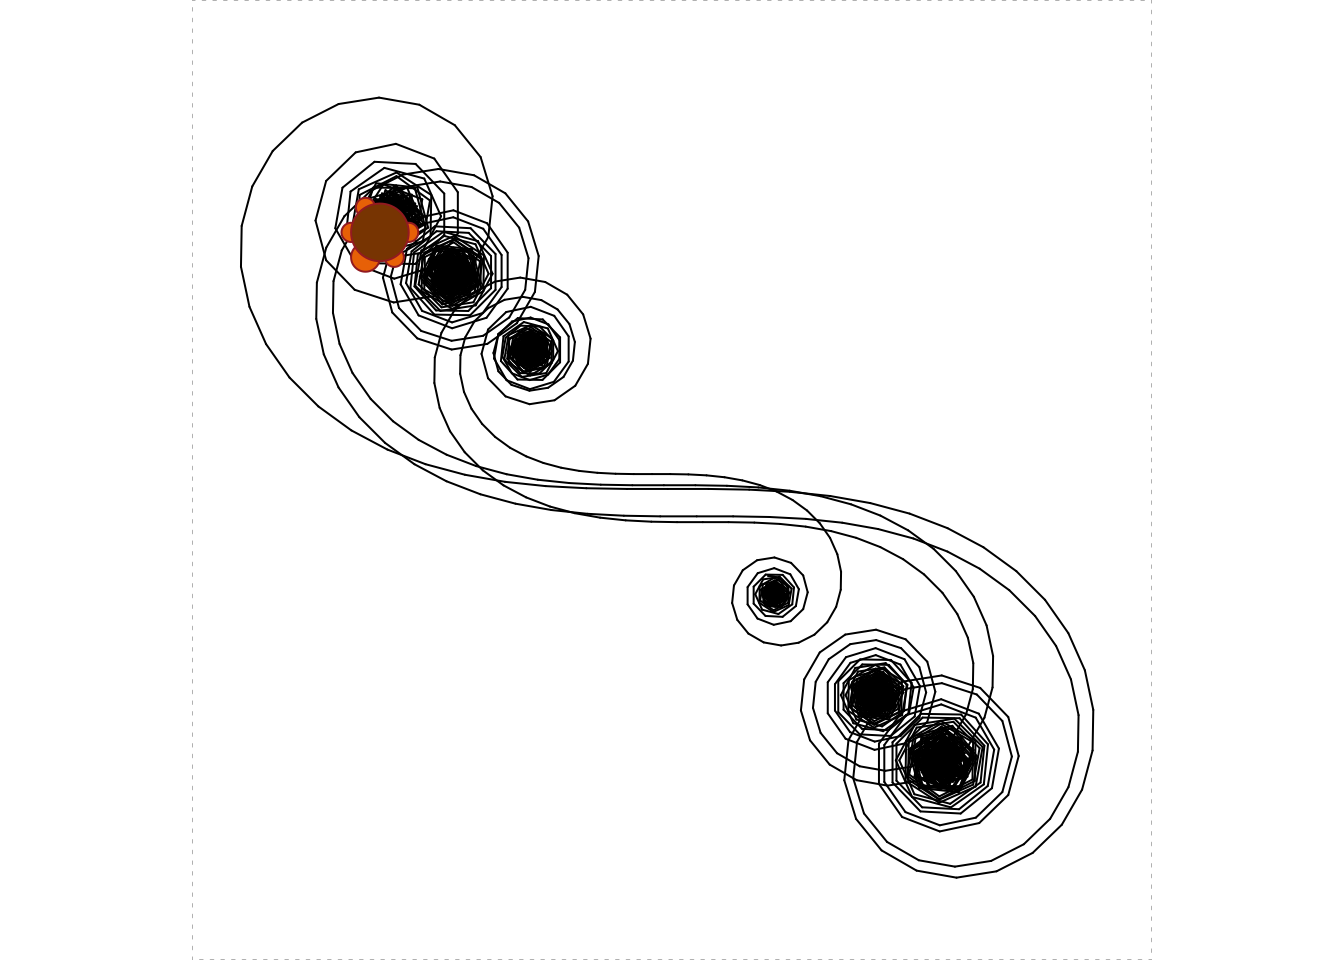
\includegraphics[width=0.5\linewidth]{r-notes_files/figure-latex/turtle-zany-1} 

}

\caption{Galactic Zany!}\label{fig:turtle-zany}
\end{figure}

You might enjoy figuring out why this pattern occurs. As you ponder
this, it might help to construct a set of ``ragged'' spirals with
somewhat larger steps, and pause at each step. Code like the following
might be useful:\footnote{Also don't forget that every 360 degrees is a
  full turn around the circle, so when the turtle's angle is, say 720
  degrees, it's the same as an angle of 360 degrees which is the same as
  an angle of 0 degrees. All three angles amount to the same direction.}

\begin{Shaded}
\begin{Highlighting}[]
\KeywordTok{turtle_init}\NormalTok{(}\DecValTok{1000}\NormalTok{, }\DecValTok{1000}\NormalTok{, }\DataTypeTok{mode =} \StringTok{"clip"}\NormalTok{)}
\KeywordTok{turtle_do}\NormalTok{(\{}
  \NormalTok{i <-}\StringTok{ }\DecValTok{1}
  \KeywordTok{turtle_right}\NormalTok{(}\DecValTok{90}\NormalTok{)}
  \NormalTok{repeat \{}
    \NormalTok{bidding <-}\StringTok{ }\KeywordTok{readline}\NormalTok{(}\StringTok{"Proceed? (Enter q to quit) "}\NormalTok{)}
    \NormalTok{if ( bidding ==}\StringTok{ "q"}\NormalTok{) break}
    \KeywordTok{turtle_right}\NormalTok{(i)}
    \KeywordTok{turtle_forward}\NormalTok{(}\DecValTok{2}\NormalTok{*}\KeywordTok{sqrt}\NormalTok{(i))}
    \KeywordTok{cat}\NormalTok{(}\KeywordTok{paste0}\NormalTok{(}\StringTok{"Turned "}\NormalTok{, i, }\StringTok{" degrees,}\CharTok{\textbackslash{}n}\StringTok{"}\NormalTok{))}
    \KeywordTok{cat}\NormalTok{(}\KeywordTok{paste0}\NormalTok{(}\StringTok{"stepped forward "}\NormalTok{, }\KeywordTok{round}\NormalTok{(}\DecValTok{2}\NormalTok{*}\KeywordTok{sqrt}\NormalTok{(i), }\DecValTok{3}\NormalTok{), }\StringTok{" units.}\CharTok{\textbackslash{}n}\StringTok{"}\NormalTok{))}
    \KeywordTok{cat}\NormalTok{(}\StringTok{"Turtle's current angle is: "}\NormalTok{, }\KeywordTok{turtle_getangle}\NormalTok{(), }\StringTok{" degrees.}\CharTok{\textbackslash{}n}\StringTok{"}\NormalTok{)}
    \NormalTok{i <-}\StringTok{ }\NormalTok{i +}\StringTok{ }\DecValTok{20}
  \NormalTok{\}}
  \KeywordTok{cat}\NormalTok{(}\StringTok{"All done!"}\NormalTok{)}
\NormalTok{\})}
\end{Highlighting}
\end{Shaded}

\newpage

\section*{Glossary}\label{glossary-3}
\addcontentsline{toc}{section}{Glossary}

\begin{description}
\item[Pseudo-random Numbers \index{pseudo-random numbers}]
A sequence of numbers generated by a computer procedure designed to make
the sequence appear to follow statistical laws associated with random
processes in nature.
\end{description}

\newpage

\section*{Exercises}\label{exercises-3}
\addcontentsline{toc}{section}{Exercises}

\begin{center}
\includegraphics[width=0.5\linewidth]{images/thinking} \end{center}

\begin{enumerate}
\def\labelenumi{\arabic{enumi}.}
\item
  Write a function called \texttt{turtle\_gon()} that draws a regular
  polygon. The user should be able to specify the side-length and the
  number of sides. Start with \texttt{turtle\_init()} and use your
  function to draw a regular dodecagon (twelve sides) with each side
  having a side length of 115 units. Your figure should not stray
  outside of the turtle's field, so you may have to adjust the position
  of your turtle a bit prior to calling your function.
\item
  Write a function called \texttt{turtle\_star()} that can make stars
  like the ones in Figure \ref{fig:turtlestarstart}. The user should be
  able to specify:

  \begin{itemize}
  \tightlist
  \item
    the number of rays in a star (default is 6);
  \item
    the length of the rays (default is 20);
  \item
    the color of the rays (default is red);
  \item
    the line-type of the rays (default is 1);
  \item
    the line-width of the rays (default is 1).
  \end{itemize}

  \begin{figure}

  {\centering 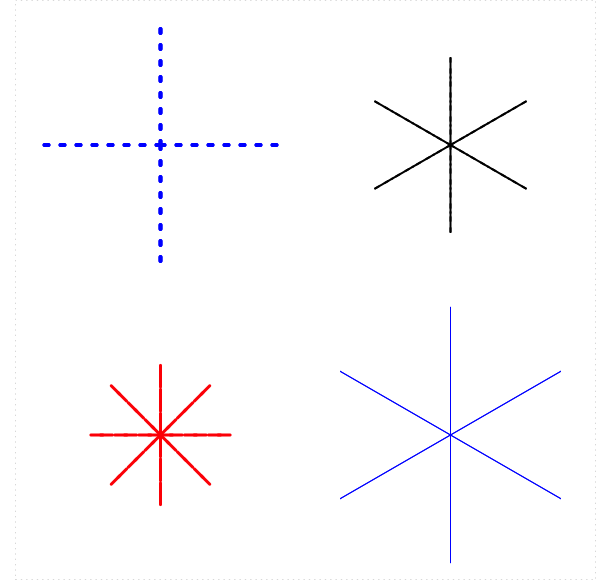
\includegraphics[width=0.6\linewidth]{images/turtle-stars} 

  }

  \caption{Sample Stars}\label{fig:turtlestarstart}
  \end{figure}

  Starting with \texttt{turtle\_init()}, use your function to create a
  star with 10 rays each of length 20 units. The lines should be red and
  dashed. I'll leave the thickness up to you.
\item
  Make a new star function \texttt{turtle\_rstar()} in which the lengths
  of the rays are not determined by the user but instead vary randomly
  from 5 to 25 units, as in Figure \ref{fig:next-turtle-star}:

  \begin{figure}

  {\centering 
\includegraphics[width=0.6\linewidth]{images/turtle-stars-2} 

  }

  \caption{A star with rays of random lengths.}\label{fig:next-turtle-star}
  \end{figure}

  The defaults for the other parameters should be the same as in the
  previous exercise. Starting from \texttt{turtle\_init(50,50)} make a
  random star with 20 rays and a line-thickness of 3. Other parameters
  should be left at their default-values.
\item
  Make a new star function \texttt{turtle\_rstarColors()} that behaves
  like \texttt{turtle\_rstar()} except that instead of being determined
  by the user the ray-color varies randomly from one ray to another, as
  in Figure \ref{fig:turtle-star-3}:

  \begin{figure}

  {\centering 
\includegraphics[width=0.6\linewidth]{images/turtle-stars-3} 

  }

  \caption{A star with rays of random lengths and random colors.}\label{fig:turtle-star-3}
  \end{figure}

  Each ray should have a color drawn randomly from the vector of all
  colors given by \texttt{colors()}. Starting from
  \texttt{turtle\_init(50,50)} make a random star with 20 rays and a
  line-thickness of 6. Other parameters should be left at their
  default-values.
\end{enumerate}

\chapter{Simulation}\label{simulation}

\begin{figure}[!h]

{\centering 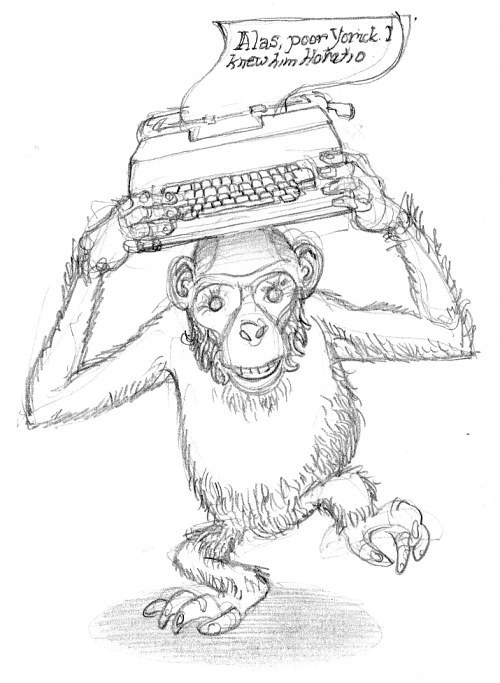
\includegraphics[width=0.4\linewidth]{images/monkey-typewriter} 

}

\caption{A monkey typing randomly manages to type out a line of Shakespeare.  What is the chance that the monky would produce this particular line?  Source: http://www.gloryofkings.com/?p=189.}\label{fig:monkey-typewriter}
\end{figure}

\newpage

\section{Probability and Random
Variables}\label{probability-and-random-variables}

Your favorite college basketball team is in the NCAA Tournament. What is
the chance that it will make the Final Four?

An insurance company provides flood insurance to homeowners. How much
can the company expect to pay out in insurance claims in the coming
year?

What is the chance of a large asteroid striking our planet in the next
ten years? in the next ten million years?

All of the above questions involve random processes---some of them
rather complex. It is the aim of this Chapter to apply our knowledge of
vectors, functions and flow control to give approximate answers to
questions involving chance processes like these.

Sometimes we will be interested in finding the \emph{probability} that
an event of interest occurs: for example, the event that your team makes
the final Four, or the event that the Earth is struck by a large
asteroid sometime in the next ten years.

One popular definition of probability \index{probability}goes as
follows:

\begin{quote}
If \(E\) is an event, then the probability that \(E\) occurs is the
long-term proportion of times that the event occurs, if we could repeat
the random process many, many times.
\end{quote}

To be more precise, imagine that you can repeat the random process \(n\)
times. (Imagine that your team gets into the NCAA Tournament \(n\)
times, for example.) Each time, the event of interest will either occur
or not occur. Count the number of times that the event occurs. Then
divide by \(n\). You now have the \emph{proportion} of times that it
occurred. Now imagine that \(n\) gets larger and larger. Our intuition
says that the proportion of times that the event occurs will stabilize
at some number between 0 and 1. This number is the \emph{probability}
that the event occurs. occurs.

We will also concern ourselves with \emph{random variables}.
\index{random variable}A random variable is simply a number whose value
is determined by the outcome of a chance process. The amount that the
insurance company will pay out in the next year is an example of a
random variable: its value depends on a complex chance process---how
many homeowners experience a flood, how damaging each flood is, etc.

When it comes to random variables, we are often interested in what it
might turn out to be \emph{on average}. That is, suppose we could repeat
the random process many, many times---say \(n\) times, where \(n\) is
some large number. (Suppose that we could observe the insurance company
for many, many years, with each year being the same in terms of how many
people are insured, how much their houses are worth, what the climate is
like, and so on.) Each time the process is repeated, we get a value for
the random variable. We end up with \(n\) values. Now add up these
values and divide by \(n\). We have computed their average---the mean,
as it is properly called. Now imagine that \(n\) could be larger and
larger, without bound.

\begin{quote}
The \emph{expected value} \index{expected value}of the random variable
is the number that this average converges to.
\end{quote}

In other words, the expected value of a random variable is what we
expect to get on average, in the long run, if we could repeat the random
process that produces the value many, many times.

\section{Monte Carlo Simulation}\label{monte-carlo-simulation}

Our definitions of probability and expected value both involved a
limiting notion, namely: what would happen if you could somehow repeat
the random process more and more times, without a bound on the number of
repetitions. Accordingly, even if we find that we are unable to compute
a probability or an expected value exactly with mathematics, we can
still attempt to estimate it by \textbf{making the computer} repeat the
random experiment many times, keeping track of the result of the
experiment each time. This technique is known as \emph{Monte Carlo}
simulation, after the famous
\href{https://en.wikipedia.org/wiki/Monte_Carlo_Casino}{Monte Carlo
casino} in the Principality of Monaco.

In this section we will employ Monte Carlo simulation to estimate
probability and expected value in a couple of simple examples.

\subsection{Estimating a Probability}\label{estimating-a-probability}

Consider a box that holds ten tickets. Three of them are labeled with
the letter ``a''; the rest are labeled ``b'':

\begin{Shaded}
\begin{Highlighting}[]
\NormalTok{tickets <-}\StringTok{ }\KeywordTok{c}\NormalTok{(}\KeywordTok{rep}\NormalTok{(}\StringTok{"a"}\NormalTok{, }\DecValTok{3}\NormalTok{), }\KeywordTok{rep}\NormalTok{(}\StringTok{"b"}\NormalTok{, }\DecValTok{7}\NormalTok{))}
\NormalTok{tickets}
\end{Highlighting}
\end{Shaded}

\begin{verbatim}
##  [1] "a" "a" "a" "b" "b" "b" "b" "b" "b" "b"
\end{verbatim}

We plan to draw one of these tickets at random from the box, with each
ticket having the same chance to be the ticket selected. Three of the
ten tickets are a's, so our intuition says that the probability of
selecting an ``a'' ticket is 3 out of 10, or 0.3. Let's use Monte Carlo
simulation to estimate the probability, and see if we get something
close to 0.3.

In order to set up the simulation, we need a device for repeating the
random process as many times as we would like. At each repetition, the
outcome of the chance process should not depend on previous outcomes. We
can accomplish this by using R s \texttt{sample()} function
\index{R-functions!sample()@\texttt{sample()}} on the \texttt{tickets}
variable. For example, if we would like to repeat the process of
selecting a ticket twenty times, we could write the following code:

\begin{Shaded}
\begin{Highlighting}[]
\NormalTok{sims <-}\StringTok{ }\KeywordTok{sample}\NormalTok{(tickets, }\DataTypeTok{size =} \DecValTok{20}\NormalTok{, }\DataTypeTok{replace =} \OtherTok{TRUE}\NormalTok{)}
\NormalTok{sims}
\end{Highlighting}
\end{Shaded}

\begin{verbatim}
##  [1] "b" "b" "b" "a" "b" "b" "b" "b" "b" "b" "a" "a" "b" "b" "b" "b" "b"
## [18] "b" "a" "a"
\end{verbatim}

Notice that we set \texttt{replace} to \texttt{TRUE}. This was
important, since it guarantees that at each selection there are three
``a'''s and seven ``b'''s in the box, keeping the chance of getting an
``a''-ticket the same each time.

We can summarize the results in a table using R's \texttt{table()}
function: \index{R-functions!table()@\texttt{table()}}

\begin{Shaded}
\begin{Highlighting}[]
\KeywordTok{table}\NormalTok{(sims)}
\end{Highlighting}
\end{Shaded}

\begin{verbatim}
## sims
##  a  b 
##  5 15
\end{verbatim}

Of course we don't care so much about the \emph{number} of times we got
an ``a''-ticket. Instead we care about the \emph{proportion} of times we
did so. In order to convert the numbers in a table to proportions we can
make the table an argument for the function \texttt{prop.table()}:
\index{R-functions!prop.table()@\texttt{prop.table()}}

\begin{Shaded}
\begin{Highlighting}[]
\KeywordTok{prop.table}\NormalTok{(}\KeywordTok{table}\NormalTok{(sims))}
\end{Highlighting}
\end{Shaded}

\begin{verbatim}
## sims
##    a    b 
## 0.25 0.75
\end{verbatim}

Based on twenty repetitions of the random process, our estimate of the
chance an ``a''-ticket is 0.25. That's not so close to the true chance
of \(1/3\). In order to obtain a more accurate estimate, we should
increase the number of repetitions of the random process. Let's try
again, with ten thousand repetitions:

\begin{Shaded}
\begin{Highlighting}[]
\KeywordTok{set.seed}\NormalTok{(}\DecValTok{4040}\NormalTok{)}
\NormalTok{sims <-}\StringTok{ }\KeywordTok{sample}\NormalTok{(tickets, }\DataTypeTok{size =} \DecValTok{10000}\NormalTok{, }\DataTypeTok{replace =} \NormalTok{T)}
\KeywordTok{prop.table}\NormalTok{(}\KeywordTok{table}\NormalTok{(sims))}
\end{Highlighting}
\end{Shaded}

\begin{verbatim}
## sims
##     a     b 
## 0.308 0.692
\end{verbatim}

Our estimate is now a lot closer to the actual value of the probability.

\subsection{Estimating an Expected
Value}\label{estimating-an-expected-value}

Imagine that you are about to play the following game: you will flip a
fair coin twice.

\begin{itemize}
\tightlist
\item
  If you get Tails both times, you lose a dollar.
\item
  If you get exactly one Head, nothing happens.
\item
  If you get Heads both times, you win two dollars.
\end{itemize}

Let \(W\) be the number of dollars you will win.

\(W\) is a clearly a random variable: it's a number whose value---either
-1, 0 or 2---depends on the outcome of the random process of flipping
the fair coin twice. What is the expected value of \(W\)?

If we think about the probabilities involved then we can come up with a
candidate for the expected value. When you flip a fair coin twice, there
are four equally likely outcomes:

\begin{itemize}
\tightlist
\item
  Tails and then Tails (\(W = -1\))
\item
  Tails and then Heads (\(W = 0\))
\item
  Heads and then Tails (\(W = 0\))
\item
  Heads and then Heads (\(W = 2\))
\end{itemize}

Hence you have:

\begin{itemize}
\tightlist
\item
  The chance that \(W=-1\) is 0.25.
\item
  The chance that \(W=0\) is 0.50.
\item
  The chance that \(W=2\) is 0.25.
\end{itemize}

Hence the expected value should be the \emph{weighted average}:

\[0.25 \times -1 + 0.50 \times 0 + 0.25 \times 2.\] This works out to
0.25, or 25 cents.

We would like to see if Monte Carlo simulation can render an estimate
that is close to this value.

For a simple game like ours where there are only a few possible outcomes
for the random variable, it is still a good idea to use
\texttt{sample()} to simulate the random process of playing the game. We
only need to provide a vector of possible values for \(W\) to sample
from, and a vector of probabilities for obtaining each of those possible
values. The following code illustrates how we might simulate playing the
game ten times:

\begin{Shaded}
\begin{Highlighting}[]
\NormalTok{px <-}\StringTok{ }\KeywordTok{c}\NormalTok{(}\FloatTok{0.25}\NormalTok{, }\FloatTok{0.50}\NormalTok{, }\FloatTok{0.25}\NormalTok{)}
\NormalTok{winnings <-}\StringTok{ }\KeywordTok{sample}\NormalTok{(x, }\DataTypeTok{size =} \DecValTok{10}\NormalTok{, }\DataTypeTok{replace =} \NormalTok{T, }\DataTypeTok{prob =} \NormalTok{px)}
\NormalTok{winnings}
\end{Highlighting}
\end{Shaded}

\begin{verbatim}
##  [1]  0  0 -1 -1  2  0  0  0  2 -1
\end{verbatim}

The Monte Carlo estimate of the expected value of \(W\) is just the
average of the winnings in our simulations:

\begin{Shaded}
\begin{Highlighting}[]
\KeywordTok{mean}\NormalTok{(winnings)}
\end{Highlighting}
\end{Shaded}

\begin{verbatim}
## [1] 0.1
\end{verbatim}

Of course, with such a small number of repetitions of the game we cannot
expect the Monte Carlo estimate to be very accurate. Let's try again,
but with ten thousand repetitions:

\begin{Shaded}
\begin{Highlighting}[]
\NormalTok{winnings <-}\StringTok{ }\KeywordTok{sample}\NormalTok{(x, }\DataTypeTok{size =} \DecValTok{10000}\NormalTok{, }\DataTypeTok{replace =} \NormalTok{T, }\DataTypeTok{prob =} \NormalTok{px)}
\KeywordTok{mean}\NormalTok{(winnings)}
\end{Highlighting}
\end{Shaded}

\begin{verbatim}
## [1] 0.2435
\end{verbatim}

Yes, that's much closer to our mathematically-computed value!

By the way, R can easily compute the weighted average itself:

\begin{Shaded}
\begin{Highlighting}[]
\KeywordTok{sum}\NormalTok{(x*px)}
\end{Highlighting}
\end{Shaded}

\begin{verbatim}
## [1] 0.25
\end{verbatim}

\subsection{The Law of Large Numbers}\label{the-law-of-large-numbers}

In our Monte Carlo simulations so far, we have seen that the more times
we repeat the underlying random process, the closer our estimate is
likely to be to the actual value, no matter whether we were estimating
the probability of an event or an expected value for a random variable.

This is no accident: in fact, it is a consequence of a theorem in the
subject of probability that is known as the \emph{Law of Large Numbers}.
We do not possess the mathematical machinery necessary to state the Law
precisely---much less prove it---but we can take the rough statement
given here as an assurance that the more repetitions we include in our
simulation, the more accurate the resulting estimate is liable to be.

\section{Example: Chance of a Triangle}\label{triangle-chance}

In the examples considered so far, intuition or a simple calculation
suggests what the exact value of the probability or expected value
should be. The true power of the Monte Carlo simulation method shines
forth in situations where it is difficult or impossible to compute a
value mathematically.

Let's revisit an example from Section \ref{ifelse}, where we considered
whether or not three segments could be put together to form a triangle.
We developed the following function to determine, from the lengths of
each segment, whether or not a triangle is possible:

\begin{Shaded}
\begin{Highlighting}[]
\NormalTok{isTriangle <-}\StringTok{ }\NormalTok{function(x, y, z) \{}
  \NormalTok{(x +}\StringTok{ }\NormalTok{y >}\StringTok{ }\NormalTok{z) &}\StringTok{ }\NormalTok{(x +z >}\StringTok{ }\NormalTok{y) &}\StringTok{ }\NormalTok{(y +}\StringTok{ }\NormalTok{z >}\StringTok{ }\NormalTok{x)}
\NormalTok{\}}
\end{Highlighting}
\end{Shaded}

Recall also that this function applied to vectors of any length, so we
can use it to decide about many triples of segments at once.

Let's now inject some chance variation into the situation. Suppose that
you have a stick that is one unit in length: one foot, one meter, one
yard---whatever. You plan to break the stick at two randomly selected
points. Breaking the stick will yield three pieces. You wonder: what is
the chance that these three pieces can form a triangle?

In an advanced probability course you can show that the probability of a
triangle is exactly \(1/4\). Here we would like to estimate the
probability with Monte Carlo simulation.

In order to carry out the simulation, we will need to develop code that
produces a pair of break-points, any number of times that we
like---let's think about ten times, to start.

This is not so difficult if we use the \texttt{runif()} function:

\begin{Shaded}
\begin{Highlighting}[]
\NormalTok{x <-}\StringTok{ }\KeywordTok{runif}\NormalTok{(}\DecValTok{10}\NormalTok{)  }\CommentTok{# the first breaks}
\NormalTok{y <-}\StringTok{ }\KeywordTok{runif}\NormalTok{(}\DecValTok{10}\NormalTok{)  }\CommentTok{# the second breaks}
\end{Highlighting}
\end{Shaded}

Next we must compute---for each pair of breaks---the lengths of the
three segments that are produced. If we knew that the \texttt{x} break
was always less than the \texttt{y} break, this would be easy:

\begin{itemize}
\tightlist
\item
  the leftmost piece would be \texttt{x} units long;
\item
  the middle piece would be \texttt{y} minus \texttt{x} units long;
\item
  the rightmost piece would be 1 minus \texttt{y} units long.
\end{itemize}

The problem is that a given element of the vector \texttt{y} can easily
be less than than corresponding element of the vector \texttt{x}. When
that happens, the pieces won't be as described in the bullet-ed items
above.

We can solve this problem with the \texttt{pmin()} and \texttt{pmax()}
functions \index{R-functions!pmin()@\texttt{pmin()}}
\index{R-functions!pmax()@\texttt{pmax()}}that were introduced in
Section \ref{maxmin}:

\begin{Shaded}
\begin{Highlighting}[]
\NormalTok{a <-}\StringTok{ }\KeywordTok{pmin}\NormalTok{(x, y)}
\NormalTok{b <-}\StringTok{ }\KeywordTok{pmax}\NormalTok{(x, y)}
\NormalTok{side1 <-}\StringTok{ }\NormalTok{a     }\CommentTok{# leftmost}
\NormalTok{side2 <-}\StringTok{ }\NormalTok{b -}\StringTok{ }\NormalTok{a  }\CommentTok{# middle}
\NormalTok{side3 <-}\StringTok{ }\DecValTok{1} \NormalTok{-}\StringTok{ }\NormalTok{b }\CommentTok{# rigttmost}
\end{Highlighting}
\end{Shaded}

It is useful to write a helper-function that starts from the breaks,
computes the sides, and then decides whether they form a triangle:

\begin{Shaded}
\begin{Highlighting}[]
\NormalTok{makesTriangle <-}\StringTok{ }\NormalTok{function(x, y) \{}
  \NormalTok{a <-}\StringTok{ }\KeywordTok{pmin}\NormalTok{(x, y)}
  \NormalTok{b <-}\StringTok{ }\KeywordTok{pmax}\NormalTok{(x, y)}
  \NormalTok{side1 <-}\StringTok{ }\NormalTok{a}
  \NormalTok{side2 <-}\StringTok{ }\NormalTok{b -}\StringTok{ }\NormalTok{a}
  \NormalTok{side3 <-}\StringTok{ }\DecValTok{1} \NormalTok{-}\StringTok{ }\NormalTok{b}
  \KeywordTok{isTriangle}\NormalTok{(}\DataTypeTok{x =} \NormalTok{side1, }\DataTypeTok{y =} \NormalTok{side2, }\DataTypeTok{z =} \NormalTok{side3)}
\NormalTok{\}}
\end{Highlighting}
\end{Shaded}

Let's try it our for our repetitions

Table \ref{tab:trianglesimstab} shows the results. Based on our ten
repetitions, we would estimate the probability of a triangle as
\(4/10\).

\begin{table}

\caption{\label{tab:trianglesimstab}Results of ten repetitions of breaking a unit length at two random points to form three segments.}
\centering
\begin{tabular}[t]{r|r|r|r|r|l}
\hline
x & y & side1 & side2 & side3 & triangle\\
\hline
0.6469028 & 0.7644140 & 0.6469028 & 0.1175112 & 0.2355860 & FALSE\\
\hline
0.3942258 & 0.7438358 & 0.3942258 & 0.3496100 & 0.2561642 & TRUE\\
\hline
0.6185018 & 0.8261657 & 0.6185018 & 0.2076639 & 0.1738343 & FALSE\\
\hline
0.4768911 & 0.4227291 & 0.4227291 & 0.0541621 & 0.5231089 & FALSE\\
\hline
0.1360972 & 0.4092877 & 0.1360972 & 0.2731905 & 0.5907123 & FALSE\\
\hline
0.0673844 & 0.5396926 & 0.0673844 & 0.4723082 & 0.4603074 & TRUE\\
\hline
0.1291526 & 0.9607224 & 0.1291526 & 0.8315698 & 0.0392776 & FALSE\\
\hline
0.3931179 & 0.6535573 & 0.3931179 & 0.2604394 & 0.3464427 & TRUE\\
\hline
0.0025827 & 0.5467153 & 0.0025827 & 0.5441326 & 0.4532847 & FALSE\\
\hline
0.6202060 & 0.2660636 & 0.2660636 & 0.3541424 & 0.3797940 & TRUE\\
\hline
\end{tabular}
\end{table}

Interestingly, R can compute the proportion of times that a triangle was
formed directly from the logical vector \texttt{triangle}. Look at the
following code:

\begin{Shaded}
\begin{Highlighting}[]
\KeywordTok{sum}\NormalTok{(triangle)}
\end{Highlighting}
\end{Shaded}

\begin{verbatim}
## [1] 4
\end{verbatim}

\begin{Shaded}
\begin{Highlighting}[]
\KeywordTok{mean}\NormalTok{(triangle)}
\end{Highlighting}
\end{Shaded}

\begin{verbatim}
## [1] 0.4
\end{verbatim}

When we ask R to add the elements of a logical vector, it coerces the
Boolean values to numbers: \texttt{TRUE} becomes 1 and \texttt{FALSE}
becomes 0. Summing the numbers is then equivalent to counting how many
times \texttt{TRUE} appeared in \texttt{triangle}. Taking the mean is
equivalent to computing the proportion of \texttt{TRUE}s in
\texttt{triangle}.

We would like, of course, to simulate breaking the unit length many
times, and we would like to be able to choose easily---without a lot of
fuss in coding---the number of repetitions. It makes sense, therefore,
to write a simulation function that will do our work for us:

\begin{Shaded}
\begin{Highlighting}[]
\NormalTok{triangleSim <-}\StringTok{ }\NormalTok{function(}\DataTypeTok{reps =} \DecValTok{10000} \NormalTok{) \{}
  \NormalTok{cut1 <-}\StringTok{ }\KeywordTok{runif}\NormalTok{(reps)}
  \NormalTok{cut2 <-}\StringTok{ }\KeywordTok{runif}\NormalTok{(reps)}
  \NormalTok{triangle <-}\StringTok{ }\KeywordTok{makesTriangle}\NormalTok{(cut1, cut2)}
  \KeywordTok{cat}\NormalTok{(}\StringTok{"The proportion of triangles was "}\NormalTok{, }\KeywordTok{mean}\NormalTok{(triangle), }\StringTok{".}\CharTok{\textbackslash{}n}\StringTok{"}\NormalTok{, }\DataTypeTok{sep =} \StringTok{""}\NormalTok{)}
\NormalTok{\}}
\end{Highlighting}
\end{Shaded}

Now that we think about it, it might also be nice to have the option to
view a table of the results, along with the estimate of the probability:

\begin{Shaded}
\begin{Highlighting}[]
\NormalTok{triangleSim <-}\StringTok{ }\NormalTok{function(}\DataTypeTok{reps =} \DecValTok{10000}\NormalTok{, }\DataTypeTok{table =} \OtherTok{FALSE} \NormalTok{) \{}
  \NormalTok{cut1 <-}\StringTok{ }\KeywordTok{runif}\NormalTok{(reps)}
  \NormalTok{cut2 <-}\StringTok{ }\KeywordTok{runif}\NormalTok{(reps)}
  \NormalTok{triangle <-}\StringTok{ }\KeywordTok{makesTriangle}\NormalTok{(cut1, cut2)}
  \NormalTok{if ( table ) \{}
    \KeywordTok{cat}\NormalTok{(}\StringTok{"Here is a table of the results:}\CharTok{\textbackslash{}n}\StringTok{"}\NormalTok{)}
    \KeywordTok{print}\NormalTok{(}\KeywordTok{table}\NormalTok{(triangle))}
    \KeywordTok{cat}\NormalTok{(}\StringTok{"}\CharTok{\textbackslash{}n}\StringTok{"}\NormalTok{)}
  \NormalTok{\}}
  \KeywordTok{cat}\NormalTok{(}\StringTok{"The proportion of triangles was "}\NormalTok{, }\KeywordTok{mean}\NormalTok{(triangle), }\StringTok{".}\CharTok{\textbackslash{}n}\StringTok{"}\NormalTok{, }\DataTypeTok{sep =} \StringTok{""}\NormalTok{)}
\NormalTok{\}}
\end{Highlighting}
\end{Shaded}

Let's give our function a try, using the default of ten thousand
repetitions and asking for a table of results:

\begin{Shaded}
\begin{Highlighting}[]
\KeywordTok{triangleSim}\NormalTok{(}\DataTypeTok{table =} \OtherTok{TRUE}\NormalTok{)}
\end{Highlighting}
\end{Shaded}

\begin{verbatim}
## Here is a table of the results:
## triangle
## FALSE  TRUE 
##  7466  2534 
## 
## The proportion of triangles was 0.2534.
\end{verbatim}

As we would expect, our estimate of the probability of a triangle is
pretty close to \(1/4\), the value that is known to experts in
probability.

\subsection{Setting a Seed}\label{setting-a-seed}

There are further possibilities for refining the simulation function. We
know that it can be a good idea to set a seed for R's random-number
generator. When you do this you still get random-looking results, but
they will be the same results no matter how often you call the
simulation function. In that way others who have access to your function
can ``reproduce'' the results you got, thus assuring themselves that you
weren't making anything up. Let's add a \texttt{seed} parameter to our
simulation function:

\begin{Shaded}
\begin{Highlighting}[]
\NormalTok{triangleSim <-}\StringTok{ }\NormalTok{function(}\DataTypeTok{reps =} \DecValTok{10000}\NormalTok{, }\DataTypeTok{table =} \OtherTok{FALSE}\NormalTok{, seed ) \{}
  \NormalTok{cut1 <-}\StringTok{ }\KeywordTok{runif}\NormalTok{(reps)}
  \NormalTok{cut2 <-}\StringTok{ }\KeywordTok{runif}\NormalTok{(reps)}
  \NormalTok{triangle <-}\StringTok{ }\KeywordTok{makesTriangle}\NormalTok{(cut1, cut2)}
  \NormalTok{if ( table ) \{}
    \KeywordTok{cat}\NormalTok{(}\StringTok{"Here is a table of the results:}\CharTok{\textbackslash{}n\textbackslash{}n}\StringTok{"}\NormalTok{)}
    \KeywordTok{print}\NormalTok{(}\KeywordTok{table}\NormalTok{(triangle))}
    \KeywordTok{cat}\NormalTok{(}\StringTok{"}\CharTok{\textbackslash{}n}\StringTok{"}\NormalTok{)}
  \NormalTok{\}}
  \KeywordTok{cat}\NormalTok{(}\StringTok{"The proportion of triangles was "}\NormalTok{, }\KeywordTok{mean}\NormalTok{(triangle), }\StringTok{".}\CharTok{\textbackslash{}n}\StringTok{"}\NormalTok{, }\DataTypeTok{sep =} \StringTok{""}\NormalTok{)}
\NormalTok{\}}
\end{Highlighting}
\end{Shaded}

This is all very well, but if for some reason you \emph{desire} to have
the function produce different results with every call, you have to come
up with the seed yourself. It would be nice to have the option to call
your function without having to provide a seed.

We would like to force R to provide a seed when it is not given one to
use. Such a seed should vary from one call to another in a way that
cannot be predicted easily.

I suggest the use of the \texttt{Sys.time()}
function\index{R-functions!Sys.time()@\texttt{Sys.time()}}, which gives
your computer's idea of the current time:

\begin{Shaded}
\begin{Highlighting}[]
\KeywordTok{Sys.time}\NormalTok{()}
\end{Highlighting}
\end{Shaded}

\begin{verbatim}
## [1] "2017-07-17 14:04:39 EDT"
\end{verbatim}

This is not a number, but we can make it a number:

\begin{Shaded}
\begin{Highlighting}[]
\KeywordTok{as.numeric}\NormalTok{(}\KeywordTok{Sys.time}\NormalTok{())}
\end{Highlighting}
\end{Shaded}

\begin{verbatim}
## [1] 1500314680
\end{verbatim}

The result is---on Unix-like computer systems---the number of seconds
elapsed since January 1, 1970. It should serve pretty well as a seed.
The following code implements a \texttt{seed} parameter in such a way
that the system-time is used when the user does not supply a seed.

\begin{Shaded}
\begin{Highlighting}[]
\NormalTok{triangleSim <-}\StringTok{ }\NormalTok{function(}\DataTypeTok{reps =} \DecValTok{10000}\NormalTok{, }\DataTypeTok{table =} \OtherTok{FALSE}\NormalTok{, }\DataTypeTok{seed =} \OtherTok{NULL}\NormalTok{) \{}
  \CommentTok{# if user does not provide a seed, set one}
  \CommentTok{# using the current time:}
  \NormalTok{if ( }\KeywordTok{is.null}\NormalTok{(seed) ) \{}
    \NormalTok{seed <-}\StringTok{ }\KeywordTok{as.numeric}\NormalTok{(}\KeywordTok{Sys.time}\NormalTok{())}
  \NormalTok{\}}
  \CommentTok{# now we can set the seed:}
  \KeywordTok{set.seed}\NormalTok{(seed)}
  
  \NormalTok{cut1 <-}\StringTok{ }\KeywordTok{runif}\NormalTok{(reps)}
  \NormalTok{cut2 <-}\StringTok{ }\KeywordTok{runif}\NormalTok{(reps)}
  \NormalTok{triangle <-}\StringTok{ }\KeywordTok{makesTriangle}\NormalTok{(cut1, cut2)}
  \NormalTok{if ( table ) \{}
    \KeywordTok{cat}\NormalTok{(}\StringTok{"Here is a table of the results:}\CharTok{\textbackslash{}n\textbackslash{}n}\StringTok{"}\NormalTok{)}
    \KeywordTok{print}\NormalTok{(}\KeywordTok{table}\NormalTok{(triangle))}
    \KeywordTok{cat}\NormalTok{(}\StringTok{"}\CharTok{\textbackslash{}n}\StringTok{"}\NormalTok{)}
  \NormalTok{\}}
  \KeywordTok{cat}\NormalTok{(}\StringTok{"The proportion of triangles was "}\NormalTok{, }\KeywordTok{mean}\NormalTok{(triangle), }\StringTok{".}\CharTok{\textbackslash{}n}\StringTok{"}\NormalTok{, }\DataTypeTok{sep =} \StringTok{""}\NormalTok{)}
\NormalTok{\}}
\end{Highlighting}
\end{Shaded}

As long as you don't make the very same simulation-function call twice
in the same second, you should get different results on different calls.

\subsection{Program Development}\label{program-development}

Think about how we developed the \texttt{triangleSim()} function.

\begin{enumerate}
\def\labelenumi{\arabic{enumi}.}
\tightlist
\item
  We began by writing simple code that got us a simulation for a few
  repetitions.
\item
  When we were sure how to make a simulation work, we
  \emph{encapsulated} our code into a function that we could call to
  perform the simulation for us.
\item
  We though about features that we would like the function to
  have---user chooses number of repetitions, user chooses whether to see
  a table, etc.---and implemented these features one by one. This made
  the function more \emph{general}, i.e., useful in a wider range of
  settings.
\end{enumerate}

The above method of program development is called \emph{encapsulation
and generalization}. For small projects of the sort that we have on
hand, it's a good way to go about writing a computer program.
\index{encapsulation and generalization}

\subsection{Number of Repetitions}\label{number-of-repetitions}

The Law of Large Numbers says that the more times you repeat the
simulation, the better our estimate of the desired probability---or
expected value---is liable to be. Let's use the Stick-Splitting Problem
to investigate the effect of the choice of repetitions on the accuracy
of our estimate of the probability of getting a triangle.

We will need to run the \texttt{tringleSim()} function several times,
with a different choice for \texttt{reps} each time, keeping track of
the estimates we obtain. In the process we won't need tables or other
output to the console. Let's rewrite \texttt{triangleSim()} for maximum
flexibility, making console output optional and using the invisible
return discussed in Section \ref{invisible-returns}.\footnote{The
  addition of the invisible return may be thought of as yet another step
  in the encapsulation-and-generalization process of program
  development!}

\begin{Shaded}
\begin{Highlighting}[]
\NormalTok{triangleSim <-}\StringTok{ }\NormalTok{function(}\DataTypeTok{reps =} \DecValTok{10000}\NormalTok{, }\DataTypeTok{table =} \OtherTok{FALSE}\NormalTok{, }\DataTypeTok{seed =} \OtherTok{NULL}\NormalTok{,}
                        \DataTypeTok{verbose =} \OtherTok{TRUE}\NormalTok{) \{}
  \CommentTok{# if user does not provide a seed, set one}
  \CommentTok{# using the current time:}
  \NormalTok{if ( }\KeywordTok{is.null}\NormalTok{(seed) ) \{}
    \NormalTok{seed <-}\StringTok{ }\KeywordTok{as.numeric}\NormalTok{(}\KeywordTok{Sys.time}\NormalTok{())}
  \NormalTok{\}}
  \CommentTok{# now we can set the seed:}
  \KeywordTok{set.seed}\NormalTok{(seed)}
  
  \NormalTok{cut1 <-}\StringTok{ }\KeywordTok{runif}\NormalTok{(reps)}
  \NormalTok{cut2 <-}\StringTok{ }\KeywordTok{runif}\NormalTok{(reps)}
  \NormalTok{triangle <-}\StringTok{ }\KeywordTok{makesTriangle}\NormalTok{(cut1, cut2)}
  \NormalTok{if ( table ) \{}
    \KeywordTok{cat}\NormalTok{(}\StringTok{"Here is a table of the results:}\CharTok{\textbackslash{}n\textbackslash{}n}\StringTok{"}\NormalTok{)}
    \KeywordTok{print}\NormalTok{(}\KeywordTok{table}\NormalTok{(triangle))}
    \KeywordTok{cat}\NormalTok{(}\StringTok{"}\CharTok{\textbackslash{}n}\StringTok{"}\NormalTok{)}
  \NormalTok{\}}
  \NormalTok{if ( verbose ) \{}
    \KeywordTok{cat}\NormalTok{(}\StringTok{"The proportion of triangles was "}\NormalTok{, }\KeywordTok{mean}\NormalTok{(triangle), }\StringTok{".}\CharTok{\textbackslash{}n}\StringTok{"}\NormalTok{, }\DataTypeTok{sep =} \StringTok{""}\NormalTok{)}
  \NormalTok{\}}
  \KeywordTok{invisible}\NormalTok{(}\KeywordTok{mean}\NormalTok{(triangle))}
\NormalTok{\}}
\end{Highlighting}
\end{Shaded}

Next, we make a vector of repetitions, and a vector to hold our
estimates:

\begin{Shaded}
\begin{Highlighting}[]
\NormalTok{reps <-}\StringTok{ }\KeywordTok{c}\NormalTok{(}\DecValTok{100}\NormalTok{, }\DecValTok{1000}\NormalTok{, }\DecValTok{10000}\NormalTok{, }\DecValTok{100000}\NormalTok{, }\DecValTok{1000000}\NormalTok{)}
\NormalTok{estimates <-}\StringTok{ }\KeywordTok{numeric}\NormalTok{(}\KeywordTok{length}\NormalTok{(reps))}
\end{Highlighting}
\end{Shaded}

Next we loop through \texttt{reps}, performing a complete simulation for
each repetition-number and storing our results:

\begin{Shaded}
\begin{Highlighting}[]
\NormalTok{for ( i in }\DecValTok{1}\NormalTok{:}\KeywordTok{length}\NormalTok{(reps)) \{}
  \NormalTok{estimates[i] <-}\StringTok{ }\KeywordTok{triangleSim}\NormalTok{(}\DataTypeTok{reps =} \NormalTok{reps[i], }\DataTypeTok{seed =} \DecValTok{3030}\NormalTok{,}
                             \DataTypeTok{verbose =} \OtherTok{FALSE}\NormalTok{)}
\NormalTok{\}}
\end{Highlighting}
\end{Shaded}

Let's have a look at our estimates:

\begin{Shaded}
\begin{Highlighting}[]
\KeywordTok{names}\NormalTok{(estimates) <-}\StringTok{ }\NormalTok{reps}
\NormalTok{estimates}
\end{Highlighting}
\end{Shaded}

\begin{verbatim}
##      100     1000    10000    1e+05    1e+06 
## 0.200000 0.245000 0.254700 0.251570 0.249779
\end{verbatim}

The estimates are indeed getting closer to the theoretical value of
\(1/4\).\footnote{Statistical theory tells us that when we use Monte
  Carlo simulation to estimate a probability or an expected value, then
  the likely size of the error in the approximation is inversely
  proportional to the square root of the number of repetitions we use.
  From this it follows that to cut the likely size of the error in half
  you should increase the number of repetitions by a factor of 4. If you
  want the likely size to be one-third as big, increase repetitions by a
  factor of 9, and so on.}

\section{Example: Will They Connect?}\label{simulation-connect}

Anna and Raj make a date for coffee tomorrow at the local Coffee Shop.
After making the date, both of them forget the exact time they agreed to
meet: they can only remember that it was to be sometime between 10 and
11am. Each person, independently of the other, randomly picks a time
between 10 and 11 to arrive. If Anna arrives and Raj is not there, she
will wait up to ten minutes for him, but will leave if he does not show
within that time period. Raj is similarly disposed: he will wait ten
minutes---but no more---for Anna. What is the chance that they meet?

The key to designing a simulation procedure is to realize that Anna and
Raj will connect if and only if the difference between their arrival
times is less than 10 minutes. It doesn't matter who arrived first, so
long as the \emph{difference} is less than 10. This means that we want
to check on the \emph{absolute value} of Anna's arrival time minus Raj's
arrival time. The following code implements this idea:

\begin{Shaded}
\begin{Highlighting}[]
\NormalTok{meetupSim <-}\StringTok{ }\NormalTok{function(}\DataTypeTok{reps =} \DecValTok{10000}\NormalTok{, }\DataTypeTok{table =} \OtherTok{FALSE}\NormalTok{, }\DataTypeTok{seed =} \OtherTok{NULL}\NormalTok{) \{}
  \NormalTok{if ( }\KeywordTok{is.null}\NormalTok{(seed) ) \{}
    \NormalTok{seed <-}\StringTok{ }\KeywordTok{as.numeric}\NormalTok{(}\KeywordTok{Sys.time}\NormalTok{())}
  \NormalTok{\}}
  \KeywordTok{set.seed}\NormalTok{(seed)}
  \NormalTok{anna <-}\StringTok{ }\KeywordTok{runif}\NormalTok{(reps, }\DecValTok{0}\NormalTok{, }\DecValTok{60}\NormalTok{)}
  \NormalTok{raj <-}\StringTok{ }\KeywordTok{runif}\NormalTok{(reps, }\DecValTok{0}\NormalTok{, }\DecValTok{60}\NormalTok{)}
  \NormalTok{connect <-}\StringTok{ }\NormalTok{(}\KeywordTok{abs}\NormalTok{(anna -}\StringTok{ }\NormalTok{raj) <}\StringTok{ }\DecValTok{10}\NormalTok{)}
  \NormalTok{if ( table ) \{}
    \KeywordTok{cat}\NormalTok{(}\StringTok{"Here is a table of the results:}\CharTok{\textbackslash{}n\textbackslash{}n}\StringTok{"}\NormalTok{)}
    \KeywordTok{print}\NormalTok{(}\KeywordTok{table}\NormalTok{(connect))}
    \KeywordTok{cat}\NormalTok{(}\StringTok{"}\CharTok{\textbackslash{}n}\StringTok{"}\NormalTok{)}
  \NormalTok{\}}
  \KeywordTok{cat}\NormalTok{(}\StringTok{"The proportion of tims they met was "}\NormalTok{, }\KeywordTok{mean}\NormalTok{(connect), }\StringTok{".}\CharTok{\textbackslash{}n}\StringTok{"}\NormalTok{, }\DataTypeTok{sep =} \StringTok{""}\NormalTok{)}
\NormalTok{\}}
\end{Highlighting}
\end{Shaded}

Let's try it out:

\begin{Shaded}
\begin{Highlighting}[]
\KeywordTok{meetupSim}\NormalTok{(}\DataTypeTok{reps =} \DecValTok{100000}\NormalTok{, }\DataTypeTok{table =} \OtherTok{TRUE}\NormalTok{, }\DataTypeTok{seed =} \DecValTok{3939}\NormalTok{)}
\end{Highlighting}
\end{Shaded}

\begin{verbatim}
## Here is a table of the results:
## 
## connect
## FALSE  TRUE 
## 69781 30219 
## 
## The proportion of tims they met was 0.30219.
\end{verbatim}

\subsection{Vectorization vs.~Looping}\label{vectorization-vs.looping}

Whenever you perform a simulation you have the option to use a
\texttt{for}-loop, running through the loop once for each repetition of
the random process in question. For example, you could rewrite the
meetup-simulation as follows:

\begin{Shaded}
\begin{Highlighting}[]
\NormalTok{meetupSim2 <-}\StringTok{ }\NormalTok{function(}\DataTypeTok{reps =} \DecValTok{10000}\NormalTok{, }\DataTypeTok{table =} \OtherTok{FALSE}\NormalTok{, }\DataTypeTok{seed =} \OtherTok{NULL}\NormalTok{) \{}
  \NormalTok{if ( }\KeywordTok{is.null}\NormalTok{(seed) ) \{}
    \NormalTok{seed <-}\StringTok{ }\KeywordTok{as.numeric}\NormalTok{(}\KeywordTok{Sys.time}\NormalTok{())}
  \NormalTok{\}}
  \CommentTok{#create an empty vector to hold the results:}
  \NormalTok{connect <-}\StringTok{ }\KeywordTok{numeric}\NormalTok{(reps)}
  \CommentTok{# loop through:}
  \NormalTok{for ( i in }\DecValTok{1}\NormalTok{:reps ) \{}
    \CommentTok{# get one arrival time for anna:}
    \NormalTok{anna <-}\StringTok{ }\KeywordTok{runif}\NormalTok{(}\DecValTok{1}\NormalTok{, }\DecValTok{0}\NormalTok{, }\DecValTok{60}\NormalTok{)}
    \CommentTok{# and one for raj:}
    \NormalTok{raj <-}\StringTok{ }\KeywordTok{runif}\NormalTok{(}\DecValTok{1}\NormalTok{, }\DecValTok{0}\NormalTok{, }\DecValTok{60}\NormalTok{)}
    \CommentTok{#compute result and record in conncect:}
    \NormalTok{connect[i] <-}\StringTok{ }\NormalTok{(}\KeywordTok{abs}\NormalTok{(anna -}\StringTok{ }\NormalTok{raj) <}\StringTok{ }\DecValTok{10}\NormalTok{)}
  \NormalTok{\}}
  \CommentTok{#the rest is the same as in meetupSim:}
  \NormalTok{if ( table ) \{}
    \KeywordTok{cat}\NormalTok{(}\StringTok{"Here is a table of the results:}\CharTok{\textbackslash{}n\textbackslash{}n}\StringTok{"}\NormalTok{)}
    \KeywordTok{print}\NormalTok{(}\KeywordTok{table}\NormalTok{(connect))}
    \KeywordTok{cat}\NormalTok{(}\StringTok{"}\CharTok{\textbackslash{}n}\StringTok{"}\NormalTok{)}
  \NormalTok{\}}
  \KeywordTok{cat}\NormalTok{(}\StringTok{"The proportion of times they met was "}\NormalTok{, }\KeywordTok{mean}\NormalTok{(connect), }\StringTok{".}\CharTok{\textbackslash{}n}\StringTok{"}\NormalTok{, }\DataTypeTok{sep =} \StringTok{""}\NormalTok{)}
\NormalTok{\}}
\end{Highlighting}
\end{Shaded}

Be aware, though, that when you use a loop in place of vectorization
your routine is liable to run more slowly. We can measure the difference
with the R-function
\texttt{system.time()}.\index{R-functions!system.time()@\texttt{system.time()}}
As an illustration, let's compare the running times for the vectorized
and the looping versions of the meetup simulation.

First we get the time for the thousand repetitions of the meetup, using
the original vectorized function:

\begin{Shaded}
\begin{Highlighting}[]
\KeywordTok{system.time}\NormalTok{(}\KeywordTok{meetupSim}\NormalTok{(}\DataTypeTok{reps =} \DecValTok{10000}\NormalTok{, }\DataTypeTok{seed =} \DecValTok{4040}\NormalTok{))}
\end{Highlighting}
\end{Shaded}

\begin{verbatim}
## The proportion of tims they met was 0.3074.
##   user  system elapsed 
##  0.002   0.001   0.003 
\end{verbatim}

Our concern is with the total elapsed time: a mere three-thousandths of
a second!

Next we get the time for the same number of repetitions, using the
looping implementation:

\begin{Shaded}
\begin{Highlighting}[]
\KeywordTok{system.time}\NormalTok{(}\KeywordTok{meetupSim2}\NormalTok{(}\DataTypeTok{reps =} \DecValTok{10000}\NormalTok{, }\DataTypeTok{seed =} \DecValTok{4040}\NormalTok{))}
\end{Highlighting}
\end{Shaded}

\begin{verbatim}
## The proportion of tims they met was 0.3084.
##    user  system elapsed 
##  0.056   0.007   0.065 
\end{verbatim}

Here the elapsed time is 0.065 seconds. This still seems pretty fast,
but it's more than 20 times as long as for the vectorized simulation.
For more complex simulations such a dramatic slowdown could pose serious
practical problems.

\BeginKnitrBlock{rmdtip}
When performance is an issue, prefer vectorization to looping as much as
possible.
\EndKnitrBlock{rmdtip}

\section{Example: the Appeals Court
Paradox}\label{appeals-court-paradox}

The following example is discussed in \citep{Nahin2008}.

An appeals court generally consists of an odd number of justices, so the
court will not be hampered with tie-votes and will thus always be able
to render a decision for any case brought before it. Let's imagine an
appeals court that has five members. Let us further imagine that for
each case before the court, each of the justices, independently of the
others, makes a decision for either one or the other of the two opposing
parties. Assume also for the sake of simplicity that there is always one
side that is ``in the right''. It follows that each judge is making a
decision that is either correct or incorrect. The judges then report
their decisions to one another, and the decision of the court is
determined by majority vote. To be precise: whichever side gets three or
more votes is the side that wins.

Although all of the members of the court are pretty sharp, they differ
somewhat in their legal abilities:

\begin{itemize}
\tightlist
\item
  In any case that comes before her, Judge A has a 95\% chance to decide
  correctly.
\item
  Judge B has a 94\% chance to judge correctly.
\item
  Judges C and D each have a 90\% chance to judge correctly.
\item
  Judge E is the weak link on the court, with a mere 80\% chance to
  judge correctly.
\end{itemize}

We are interested in estimating the probability that the majority
opinion of the court will be correct.

Before we write a simulation in full, we should consider how we are
going to simulate something that has a specified percentage chance of
happening. For example, how would we simulate decisions made by Judge A?

One approach is to use \texttt{runif()} with a cutoff:

\begin{Shaded}
\begin{Highlighting}[]
\NormalTok{number <-}\StringTok{ }\KeywordTok{runif}\NormalTok{(}\DecValTok{1}\NormalTok{) }\CommentTok{# random number between 0 and 1}
\NormalTok{number <}\StringTok{ }\FloatTok{0.95}
\end{Highlighting}
\end{Shaded}

\begin{verbatim}
## [1] FALSE
\end{verbatim}

In repeated trials, a random real number between 0 and 1 will turn out
to be less than 0.95 about 95\% of the time.

Another---and more convenient---way is to use the function
\texttt{rbinom()}. \index{R-functions!rbinom()@\texttt{rbinom()}} This
function simulates the results of flipping a coin a number of times and
counting how many heads one gets. The general form of a call to
\texttt{rbinom()}is as follows:

\begin{Shaded}
\begin{Highlighting}[]
\KeywordTok{rbinom}\NormalTok{(n, size, prob)}
\end{Highlighting}
\end{Shaded}

In this call:

\begin{itemize}
\tightlist
\item
  \texttt{size} is how many times you plan to flip the coin;
\item
  \texttt{prob} is the chance on any flip that the coin will turn up
  heads;
\item
  \texttt{n} is how many times you plan to repeat the process of
  flipping the coin \texttt{size} times (counting up the number of heads
  each time).
\end{itemize}

In order to simulate flipping a fair coin 100 times, you could ask for:

\begin{Shaded}
\begin{Highlighting}[]
\KeywordTok{rbinom}\NormalTok{(}\DataTypeTok{n =} \DecValTok{1}\NormalTok{, }\DataTypeTok{size =} \DecValTok{100}\NormalTok{, }\DataTypeTok{prob =} \FloatTok{0.5}\NormalTok{)}
\end{Highlighting}
\end{Shaded}

\begin{verbatim}
## [1] 52
\end{verbatim}

It seems that we got 52 heads!

If you want to go through the above process twenty times instead of just
doing it once, you could ask for:

\begin{Shaded}
\begin{Highlighting}[]
\KeywordTok{rbinom}\NormalTok{(}\DataTypeTok{n =} \DecValTok{20}\NormalTok{, }\DataTypeTok{size =} \DecValTok{100}\NormalTok{, }\DataTypeTok{prob =} \FloatTok{0.5}\NormalTok{)}
\end{Highlighting}
\end{Shaded}

\begin{verbatim}
##  [1] 52 49 45 57 53 60 46 53 50 54 59 47 42 45 41 56 47 57 56 49
\end{verbatim}

Nothing in \texttt{rbinom()} says that it addresses only coin-flipping.
In general it serves as a model for any situation in which:

\begin{itemize}
\tightlist
\item
  there is a fixed number of trials (e.g., flip of a coin, taking a
  free-throw shot, deciding about a court case);
\item
  each trial has two possible outcomes, often termed Success or Failure
  (e.g., coins lands heads or tails, you make the shot or you don't, you
  decide the case correctly or you don't);
\item
  the chance of the Success outcome is the same, on any trial (e.g., the
  coin always has the same chance of coming up heads, for \emph{any}
  case Judge A has a 95\% chance of being right);
\item
  the outcome of any trial is independent of the outcome of all other
  trials (e.g., making the first free throw does not increase or
  decrease one's chances of making the next free throw, etc.)
\item
  you are counting up the number of successes in your trials.
\end{itemize}

In such a situation the count of the number of successes is called a
\emph{binomial} random variable.\footnote{``Binomial'' is borrowed from
  a Greek words whose literal meaning is ``two names''---corresponding
  to the two possible outcomes of a trial.} The \texttt{size} parameter
in \texttt{rbinom()} gives the fixed number of trials. The \texttt{prob}
parameter specifies the chance of success on each trial.

In this example we would like to simulate each judge deciding about each
case. Suppose for example, that there are twenty cases. We would like to
know, for each judge and each case, whether or not the judge was correct

Suppose we were to watch Judge A making 20 decisions, recording each
time whether she was correct or not. In order to simulate the results
with R, we could ask for:

\begin{Shaded}
\begin{Highlighting}[]
\KeywordTok{rbinom}\NormalTok{(}\DataTypeTok{n =} \DecValTok{20}\NormalTok{, }\DataTypeTok{size =} \DecValTok{1}\NormalTok{, }\DataTypeTok{prob =} \FloatTok{0.95}\NormalTok{)}
\end{Highlighting}
\end{Shaded}

\begin{verbatim}
##  [1] 1 1 1 1 1 1 1 1 1 1 1 1 1 1 1 1 0 1 1 1
\end{verbatim}

In the above results, each 1 stands for a correct decision and the 0
stands for an incorrect decision.

Note that the following call would be incorrect:

\begin{Shaded}
\begin{Highlighting}[]
\KeywordTok{rbinom}\NormalTok{(}\DataTypeTok{n =} \DecValTok{1}\NormalTok{, }\DataTypeTok{size =} \DecValTok{20}\NormalTok{, }\DataTypeTok{prob =} \FloatTok{0.95}\NormalTok{)}
\end{Highlighting}
\end{Shaded}

This would give us a \emph{count} of the number of times Judge A was
correct, but it would not tell us which of the cases she judged
correctly and which she judged incorrectly.

Assuming that the court hears 20 cases, we would like to simulate the
decision of each judge in each case. We could store the results in
variables, as follows:

\begin{Shaded}
\begin{Highlighting}[]
\NormalTok{a <-}\StringTok{ }\KeywordTok{rbinom}\NormalTok{(}\DataTypeTok{n =} \DecValTok{20}\NormalTok{, }\DataTypeTok{size =} \DecValTok{1}\NormalTok{, }\DataTypeTok{prob =} \FloatTok{0.95}\NormalTok{)  }\CommentTok{# Judge A}
\NormalTok{b <-}\StringTok{ }\KeywordTok{rbinom}\NormalTok{(}\DataTypeTok{n =} \DecValTok{20}\NormalTok{, }\DataTypeTok{size =} \DecValTok{1}\NormalTok{, }\DataTypeTok{prob =} \FloatTok{0.94}\NormalTok{)  }\CommentTok{# Judge B}
\NormalTok{c <-}\StringTok{ }\KeywordTok{rbinom}\NormalTok{(}\DataTypeTok{n =} \DecValTok{20}\NormalTok{, }\DataTypeTok{size =} \DecValTok{1}\NormalTok{, }\DataTypeTok{prob =} \FloatTok{0.90}\NormalTok{)  }\CommentTok{# Judge C}
\NormalTok{d <-}\StringTok{ }\KeywordTok{rbinom}\NormalTok{(}\DataTypeTok{n =} \DecValTok{20}\NormalTok{, }\DataTypeTok{size =} \DecValTok{1}\NormalTok{, }\DataTypeTok{prob =} \FloatTok{0.90}\NormalTok{)  }\CommentTok{# Judge D}
\NormalTok{e <-}\StringTok{ }\KeywordTok{rbinom}\NormalTok{(}\DataTypeTok{n =} \DecValTok{20}\NormalTok{, }\DataTypeTok{size =} \DecValTok{1}\NormalTok{, }\DataTypeTok{prob =} \FloatTok{0.80}\NormalTok{)  }\CommentTok{# Judge E}
\end{Highlighting}
\end{Shaded}

Now we come to the key idea in coding our simulation: in order to
determine the total number of correct votes in each case, all we need to
do is \emph{add} the five vectors we created above:

\begin{Shaded}
\begin{Highlighting}[]
\NormalTok{correctVotes <-}\StringTok{ }\NormalTok{a +}\StringTok{ }\NormalTok{b +}\StringTok{ }\NormalTok{c +}\StringTok{ }\NormalTok{d +}\StringTok{ }\NormalTok{e}
\end{Highlighting}
\end{Shaded}

The court will decide correctly when the number of votes for the correct
option is at least 3. The following logical vector records this:

\begin{Shaded}
\begin{Highlighting}[]
\NormalTok{courtCorrect <-}\StringTok{ }\NormalTok{(correctVotes >=}\StringTok{ }\DecValTok{3}\NormalTok{)}
\end{Highlighting}
\end{Shaded}

Table \ref{tab:judge-votes} shows some possible results:

\begin{table}

\caption{\label{tab:judge-votes}Results of 20 simulated appeals court decisions.}
\centering
\begin{tabular}[t]{r|r|r|r|r|r|l}
\hline
A & B & C & D & E & Number Correct & Court Correct\\
\hline
1 & 1 & 1 & 0 & 0 & 3 & TRUE\\
\hline
1 & 1 & 1 & 0 & 1 & 4 & TRUE\\
\hline
1 & 1 & 1 & 1 & 1 & 5 & TRUE\\
\hline
1 & 1 & 1 & 1 & 1 & 5 & TRUE\\
\hline
1 & 1 & 1 & 1 & 1 & 5 & TRUE\\
\hline
1 & 1 & 1 & 0 & 1 & 4 & TRUE\\
\hline
1 & 1 & 1 & 1 & 1 & 5 & TRUE\\
\hline
1 & 1 & 1 & 1 & 0 & 4 & TRUE\\
\hline
1 & 1 & 1 & 1 & 1 & 5 & TRUE\\
\hline
1 & 1 & 1 & 1 & 1 & 5 & TRUE\\
\hline
1 & 1 & 1 & 0 & 1 & 4 & TRUE\\
\hline
1 & 1 & 0 & 1 & 0 & 3 & TRUE\\
\hline
1 & 1 & 1 & 1 & 1 & 5 & TRUE\\
\hline
1 & 1 & 1 & 0 & 1 & 4 & TRUE\\
\hline
0 & 1 & 1 & 1 & 1 & 4 & TRUE\\
\hline
1 & 1 & 1 & 1 & 1 & 5 & TRUE\\
\hline
1 & 1 & 1 & 1 & 1 & 5 & TRUE\\
\hline
1 & 1 & 1 & 1 & 1 & 5 & TRUE\\
\hline
1 & 1 & 1 & 1 & 0 & 4 & TRUE\\
\hline
1 & 1 & 0 & 1 & 1 & 4 & TRUE\\
\hline
\end{tabular}
\end{table}

Note that all of the court's decisions were correct, even though in a
couple of cases the correct decisions were barely in the majority.

We now have the basic idea of the simulation. In order to estimate the
probability of a correct decision, we simply need to recast our idea in
the form of a function that permits us to simulate a very large number
of imaginary court cases and that will report the results to us. Here is
the code for such a function.

\begin{Shaded}
\begin{Highlighting}[]
\NormalTok{courtSim <-}\StringTok{ }\NormalTok{function(}\DataTypeTok{reps =} \DecValTok{10000}\NormalTok{,}
                     \DataTypeTok{seed =} \OtherTok{NULL}\NormalTok{,}
                     \DataTypeTok{table =} \OtherTok{FALSE}\NormalTok{,}
                     \DataTypeTok{probs =} \KeywordTok{c}\NormalTok{(}\FloatTok{0.95}\NormalTok{, }\FloatTok{0.94}\NormalTok{, }\FloatTok{0.90}\NormalTok{, }\FloatTok{0.90}\NormalTok{, }\FloatTok{0.80}\NormalTok{)) \{}
  
  \NormalTok{if ( }\KeywordTok{is.null}\NormalTok{(seed) ) \{}
    \NormalTok{seed <-}\StringTok{ }\KeywordTok{as.numeric}\NormalTok{(}\KeywordTok{Sys.time}\NormalTok{())}
  \NormalTok{\}}
  \KeywordTok{set.seed}\NormalTok{(seed)}
  
  \CommentTok{# get the probabilities}
  \NormalTok{aProb <-}\StringTok{ }\NormalTok{probs[}\DecValTok{1}\NormalTok{]}
  \NormalTok{bProb <-}\StringTok{ }\NormalTok{probs[}\DecValTok{2}\NormalTok{]}
  \NormalTok{cProb <-}\StringTok{ }\NormalTok{probs[}\DecValTok{3}\NormalTok{]}
  \NormalTok{dProb <-}\StringTok{ }\NormalTok{probs[}\DecValTok{4}\NormalTok{]}
  \NormalTok{eProb <-}\StringTok{ }\NormalTok{probs[}\DecValTok{5}\NormalTok{]}
  
  \CommentTok{# simulate decisions of each judge:                 }
  \NormalTok{a <-}\StringTok{ }\KeywordTok{rbinom}\NormalTok{(}\DataTypeTok{n =} \NormalTok{reps, }\DataTypeTok{size =} \DecValTok{1}\NormalTok{, }\DataTypeTok{prob =} \NormalTok{aProb)}
  \NormalTok{b <-}\StringTok{ }\KeywordTok{rbinom}\NormalTok{(}\DataTypeTok{n =} \NormalTok{reps, }\DataTypeTok{size =} \DecValTok{1}\NormalTok{, }\DataTypeTok{prob =} \NormalTok{bProb)}
  \NormalTok{c <-}\StringTok{ }\KeywordTok{rbinom}\NormalTok{(}\DataTypeTok{n =} \NormalTok{reps, }\DataTypeTok{size =} \DecValTok{1}\NormalTok{, }\DataTypeTok{prob =} \NormalTok{cProb)}
  \NormalTok{d <-}\StringTok{ }\KeywordTok{rbinom}\NormalTok{(}\DataTypeTok{n =} \NormalTok{reps, }\DataTypeTok{size =} \DecValTok{1}\NormalTok{, }\DataTypeTok{prob =} \NormalTok{dProb)}
  \NormalTok{e <-}\StringTok{ }\KeywordTok{rbinom}\NormalTok{(}\DataTypeTok{n =} \NormalTok{reps, }\DataTypeTok{size =} \DecValTok{1}\NormalTok{, }\DataTypeTok{prob =} \NormalTok{eProb)}
  
  \CommentTok{# count the number of correct votes in each case:}
  \NormalTok{correctVotes <-}\StringTok{ }\NormalTok{a +}\StringTok{ }\NormalTok{b +}\StringTok{ }\NormalTok{c +}\StringTok{ }\NormalTok{d +}\StringTok{ }\NormalTok{e}
  
  \CommentTok{# determine whether court decided correctly, in each case:}
  \NormalTok{courtCorrect <-}\StringTok{ }\NormalTok{(correctVotes >=}\StringTok{ }\DecValTok{3}\NormalTok{)}
  
  \CommentTok{# record results}
  \NormalTok{if ( table ) \{}
    \KeywordTok{cat}\NormalTok{(}\StringTok{"Here is a table of the results:}\CharTok{\textbackslash{}n\textbackslash{}n}\StringTok{"}\NormalTok{)}
    \KeywordTok{print}\NormalTok{(}\KeywordTok{table}\NormalTok{(courtCorrect))}
    \KeywordTok{cat}\NormalTok{(}\StringTok{"}\CharTok{\textbackslash{}n}\StringTok{"}\NormalTok{)}
  \NormalTok{\}}
  \KeywordTok{cat}\NormalTok{(}\StringTok{"The proportion of times the court was correct was "}\NormalTok{, }
      \KeywordTok{mean}\NormalTok{(courtCorrect), }\StringTok{".}\CharTok{\textbackslash{}n}\StringTok{"}\NormalTok{, }\DataTypeTok{sep =} \StringTok{""}\NormalTok{)}
\NormalTok{\}}
\end{Highlighting}
\end{Shaded}

Let's now estimate the probability of the court rendering a correct
verdict, using one hundred thousand simulated cases:

\begin{Shaded}
\begin{Highlighting}[]
\KeywordTok{courtSim}\NormalTok{(}\DataTypeTok{reps =} \DecValTok{100000}\NormalTok{, }\DataTypeTok{seed =} \DecValTok{3838}\NormalTok{, }\DataTypeTok{table =} \NormalTok{T)}
\end{Highlighting}
\end{Shaded}

\begin{verbatim}
## Here is a table of the results:
## 
## courtCorrect
## FALSE  TRUE 
##   772 99228 
## 
## The proportion of times the court was correct was 0.99228.
\end{verbatim}

The court seems to be doing quite well! But of course this is not very
surprising: after all, most of the judges make the correct decision
almost all the time. It is interesting, though, that the chance of the
\emph{full court} rendering a correct verdict is higher than the chance
of any individual judge to be correct. There appears to be a benefit to
the voting procedure.

But things get even more interesting if we imagine that the judges
recognize, after some time, that Judge E simply isn't as sharp as Judge
A, and that they pressure him into voting whichever way Judge A votes.
``Surely'', they reason, ``since Judge A is so good this new policy will
increase our chance to hand down a correct verdict!''

We will simulate to see if the judges' reasoning is correct. All we need
to do is to count Judge A's vote twice in the sum, and not count Judge
E's vote at all:

\begin{Shaded}
\begin{Highlighting}[]
\NormalTok{correctVotes <-}\StringTok{ }\DecValTok{2}\NormalTok{*a +}\StringTok{ }\NormalTok{b +}\StringTok{ }\NormalTok{c +}\StringTok{ }\NormalTok{d}
\end{Highlighting}
\end{Shaded}

Here is the new simulation-function:

\begin{Shaded}
\begin{Highlighting}[]
\NormalTok{courtSim2 <-}\StringTok{ }\NormalTok{function(}\DataTypeTok{reps =} \DecValTok{10000}\NormalTok{,}
                     \DataTypeTok{seed =} \OtherTok{NULL}\NormalTok{,}
                     \DataTypeTok{table =} \OtherTok{FALSE}\NormalTok{,}
                     \DataTypeTok{probs =} \KeywordTok{c}\NormalTok{(}\FloatTok{0.95}\NormalTok{, }\FloatTok{0.94}\NormalTok{, }\FloatTok{0.90}\NormalTok{, }\FloatTok{0.90}\NormalTok{, }\FloatTok{0.80}\NormalTok{)) \{}
  
  \NormalTok{if ( }\KeywordTok{is.null}\NormalTok{(seed) ) \{}
    \NormalTok{seed <-}\StringTok{ }\KeywordTok{as.numeric}\NormalTok{(}\KeywordTok{Sys.time}\NormalTok{())}
  \NormalTok{\}}
  \KeywordTok{set.seed}\NormalTok{(seed)}
  
  \CommentTok{# get the probabilities}
  \NormalTok{aProb <-}\StringTok{ }\NormalTok{probs[}\DecValTok{1}\NormalTok{]}
  \NormalTok{bProb <-}\StringTok{ }\NormalTok{probs[}\DecValTok{2}\NormalTok{]}
  \NormalTok{cProb <-}\StringTok{ }\NormalTok{probs[}\DecValTok{3}\NormalTok{]}
  \NormalTok{dProb <-}\StringTok{ }\NormalTok{probs[}\DecValTok{4}\NormalTok{]}
  \NormalTok{eProb <-}\StringTok{ }\NormalTok{probs[}\DecValTok{5}\NormalTok{]}
  
  \CommentTok{# simulate decisions (this time, no need for Judge E) :             }
  \NormalTok{a <-}\StringTok{ }\KeywordTok{rbinom}\NormalTok{(}\DataTypeTok{n =} \NormalTok{reps, }\DataTypeTok{size =} \DecValTok{1}\NormalTok{, }\DataTypeTok{prob =} \NormalTok{aProb)}
  \NormalTok{b <-}\StringTok{ }\KeywordTok{rbinom}\NormalTok{(}\DataTypeTok{n =} \NormalTok{reps, }\DataTypeTok{size =} \DecValTok{1}\NormalTok{, }\DataTypeTok{prob =} \NormalTok{bProb)}
  \NormalTok{c <-}\StringTok{ }\KeywordTok{rbinom}\NormalTok{(}\DataTypeTok{n =} \NormalTok{reps, }\DataTypeTok{size =} \DecValTok{1}\NormalTok{, }\DataTypeTok{prob =} \NormalTok{cProb)}
  \NormalTok{d <-}\StringTok{ }\KeywordTok{rbinom}\NormalTok{(}\DataTypeTok{n =} \NormalTok{reps, }\DataTypeTok{size =} \DecValTok{1}\NormalTok{, }\DataTypeTok{prob =} \NormalTok{dProb)}
  
  \CommentTok{# count rhe number of correct votes in each case:}
  \NormalTok{correctVotes <-}\StringTok{ }\DecValTok{2}\NormalTok{*a +}\StringTok{ }\NormalTok{b +}\StringTok{ }\NormalTok{c +}\StringTok{ }\NormalTok{d}
  
  \CommentTok{# determine whether court decided correctly, in each case:}
  \NormalTok{courtCorrect <-}\StringTok{ }\NormalTok{(correctVotes >=}\StringTok{ }\DecValTok{3}\NormalTok{)}
  
  \CommentTok{# record results}
  \NormalTok{if ( table ) \{}
    \KeywordTok{cat}\NormalTok{(}\StringTok{"Here is a table of the results:}\CharTok{\textbackslash{}n\textbackslash{}n}\StringTok{"}\NormalTok{)}
    \KeywordTok{print}\NormalTok{(}\KeywordTok{table}\NormalTok{(courtCorrect))}
    \KeywordTok{cat}\NormalTok{(}\StringTok{"}\CharTok{\textbackslash{}n}\StringTok{"}\NormalTok{)}
  \NormalTok{\}}
  \KeywordTok{cat}\NormalTok{(}\StringTok{"The proportion of times the court was correct was "}\NormalTok{, }
      \KeywordTok{mean}\NormalTok{(courtCorrect), }\StringTok{".}\CharTok{\textbackslash{}n}\StringTok{"}\NormalTok{, }\DataTypeTok{sep =} \StringTok{""}\NormalTok{)}
\NormalTok{\}}
\end{Highlighting}
\end{Shaded}

Let's try it out:

\begin{Shaded}
\begin{Highlighting}[]
\KeywordTok{courtSim2}\NormalTok{(}\DataTypeTok{reps =} \DecValTok{100000}\NormalTok{, }\DataTypeTok{seed =} \DecValTok{3838}\NormalTok{, }\DataTypeTok{table =} \NormalTok{T)}
\end{Highlighting}
\end{Shaded}

\begin{verbatim}
## Here is a table of the results:
## 
## courtCorrect
## FALSE  TRUE 
##  1221 98779 
## 
## The proportion of times the court was correct was 0.98779.
\end{verbatim}

Hey! That's a \emph{lower} chance of success than before! The difference
is small but significant: compelling the weakest judge to vote with the
strongest judge actually \emph{decreased} the court's chance of
rendering a correct verdict overall. This circumstance is sometimes
called the Appeals Court Paradox, but it occurs in many other practical
situations. More often than you might think, the benefit of independent
voting can outweigh the advantage associated with relying solely on a
small number of ``experts.''

\section{Example: How Many Numbers
Needed?}\label{simulation-number-needed}

Let us pause for a review.

So far our examples have involved estimating a probability: the chance
for a particular event to occur. We have accomplished this with Monte
Carlo simulation:

\begin{itemize}
\tightlist
\item
  We repeated the chance process a very large number of times
\item
  On each repetition, we recorded whether or not the event occurred.
\item
  After we finished all of the repetitions, we computed the proportion
  of those repetitions in which the event \emph{did} occur.
\item
  This proportion served as our estimate of the probability for the
  event to occur.
\item
  We know that the more repetitions we arrange for, the closer our
  estimate is liable to be to the actual probability for the event to
  occur.
\end{itemize}

Let us now switch gears and take up the task of estimating the
\emph{expected value} of a random variable.

Recall that a random variable is a number whose value is the result of
some chance process. The expected value of the random variable is the
\emph{average}---the mean---of its values over many, many repetitions of
that chance process.

Let us consider the following chance process:

\begin{itemize}
\tightlist
\item
  Pick a real number \(x_1\) between 0 and 1 at random.
\item
  Pick another real number \(x_2\) at random (also between 0 and 1). Add
  it to \(x_1\).
\item
  If the sum \(x_1 + x_2\) exceeds 1, then stop.
\item
  Otherwise, pick a third real number \(x_3\), and add it to the sum of
  the previous two.
\item
  If the sum \(x_1+x_2+x_3\) exceeds 1, then stop.
\item
  Otherwise, pick a fourth real number \ldots{}
\end{itemize}

The idea is to keep on going in this way until the sum of the numbers
you have picked exceeds 1.

The random variable we are interested in is the \emph{number} of numbers
we have to pick to make the sum of those numbers exceed 1. Let us call
this random variable \(X\). As you can see, this number could be 2, or
3, or 4, or even more depending on how small the random numbers you pick
happen to be.

In order to fully grasp what is going on, it will be helpful to go
through the process of computing \(X\). The following function will do
this for us:

\begin{Shaded}
\begin{Highlighting}[]
\NormalTok{numberNeeded <-}\StringTok{ }\NormalTok{function(}\DataTypeTok{verbose =} \OtherTok{FALSE}\NormalTok{) \{}
  \NormalTok{mySum <-}\StringTok{ }\DecValTok{0}
  \NormalTok{count <-}\StringTok{ }\DecValTok{0}
  \NormalTok{while( mySum <}\StringTok{ }\DecValTok{1} \NormalTok{) \{}
    \NormalTok{number <-}\StringTok{ }\KeywordTok{runif}\NormalTok{(}\DecValTok{1}\NormalTok{)}
    \NormalTok{mySum <-}\StringTok{ }\NormalTok{mySum +}\StringTok{ }\NormalTok{number}
    \NormalTok{count <-}\StringTok{ }\NormalTok{count +}\StringTok{ }\DecValTok{1}
    \NormalTok{if ( verbose ) \{}
      \KeywordTok{cat}\NormalTok{(}\StringTok{"Just now picked "}\NormalTok{, number, }\StringTok{".}\CharTok{\textbackslash{}n}\StringTok{"}\NormalTok{, }\DataTypeTok{sep =} \StringTok{""}\NormalTok{)}
      \KeywordTok{cat}\NormalTok{(count, }\StringTok{" number(s) picked so far.}\CharTok{\textbackslash{}n}\StringTok{"}\NormalTok{, }\DataTypeTok{sep =} \StringTok{""}\NormalTok{)}
      \KeywordTok{cat}\NormalTok{(}\StringTok{"Their sum is "}\NormalTok{, mySum, }\StringTok{".}\CharTok{\textbackslash{}n\textbackslash{}n}\StringTok{"}\NormalTok{, }\DataTypeTok{sep =} \StringTok{""}\NormalTok{)}
    \NormalTok{\}}
  \NormalTok{\}}
  \NormalTok{count}
\NormalTok{\}}
\end{Highlighting}
\end{Shaded}

Call the function a few times, like this:

\begin{Shaded}
\begin{Highlighting}[]
\KeywordTok{numberNeeded}\NormalTok{(}\DataTypeTok{verbose =} \OtherTok{TRUE}\NormalTok{)}
\end{Highlighting}
\end{Shaded}

\begin{verbatim}
## Just now picked 0.2869393.
## 1 number(s) picked so far.
## Their sum is 0.2869393.
## 
## Just now picked 0.7092682.
## 2 number(s) picked so far.
## Their sum is 0.9962075.
## 
## Just now picked 0.7524099.
## 3 number(s) picked so far.
## Their sum is 1.748617.
\end{verbatim}

\begin{verbatim}
## [1] 3
\end{verbatim}

As you can see, it's quite common to need 2 or 3 numbers to make the sum
exceed 1, but sometimes, you need 4, 5 or even more numbers.

Since we are interested in the expected value of \(X\), we should repeat
the process a large number of times and compute the mean of the
\(X\)-values that we find. The following code repeats the process 1000
times:

\begin{Shaded}
\begin{Highlighting}[]
\NormalTok{needed <-}\StringTok{ }\KeywordTok{numeric}\NormalTok{(}\DecValTok{1000}\NormalTok{)}
\NormalTok{for (i in }\DecValTok{1}\NormalTok{:}\DecValTok{1000} \NormalTok{) \{}
  \NormalTok{needed[i] <-}\StringTok{ }\KeywordTok{numberNeeded}\NormalTok{()}
\NormalTok{\}}
\KeywordTok{cat}\NormalTok{(}\StringTok{"The expected number needed is about "}\NormalTok{, }
    \KeywordTok{mean}\NormalTok{(needed), }\StringTok{".}\CharTok{\textbackslash{}n}\StringTok{"}\NormalTok{, }\DataTypeTok{sep =} \StringTok{""}\NormalTok{)}
\end{Highlighting}
\end{Shaded}

\begin{verbatim}
## The expected number needed is about 2.697.
\end{verbatim}

Of course the expected value indicates what \(X\) will be \emph{on
average}. By itself it doesn't tell us about the \emph{variability} in
\(X\)---how much \(X\) tends to ``hop around'' from one repetition to
another. In order to get a sense of the variability of \(X\), we can
make a table of the results of our 1000 repetitions:

\begin{Shaded}
\begin{Highlighting}[]
\KeywordTok{table}\NormalTok{(needed)}
\end{Highlighting}
\end{Shaded}

\begin{verbatim}
## needed
##   2   3   4   5   6   7 
## 528 303 123  37   8   1
\end{verbatim}

Sure enough, we usually got 2 or 3, but higher values are certainly
possible.

For the most part we are less interested in the \emph{number} of times
we got each possible value than we are in the \emph{proportion} of times
we got each possible value. For this all we need is
\texttt{prop.table()}:

\begin{Shaded}
\begin{Highlighting}[]
\KeywordTok{prop.table}\NormalTok{(}\KeywordTok{table}\NormalTok{(needed))}
\end{Highlighting}
\end{Shaded}

\begin{verbatim}
## needed
##     2     3     4     5     6     7 
## 0.528 0.303 0.123 0.037 0.008 0.001
\end{verbatim}

The proportions serve as estimates of the \emph{probability} of getting
each of the possible values of \(X\). Such a table of proportions gives
us a sense of the \emph{distribution} of \(X\)---the chances for \(X\)
to assume each of its possible values.\footnote{Of course not all of the
  possible values for \(X\) appear on the table: the only values
  appearing are those that happened to occur in our simulation. The
  values that did not occur probably have a very small (but nonzero)
  chance of occurring.}

Now that we have the basic idea of how to accomplish the simulation, it
remains to package up our code into a nice function that will enable a
user to set the number of repetitions, set a seed, and choose reporting
options. Along the way we will generalize a bit, allowing the user to
set a target sum other than 1.

\begin{Shaded}
\begin{Highlighting}[]
\NormalTok{numberNeededSim <-}\StringTok{ }\NormalTok{function(}\DataTypeTok{target =} \DecValTok{1}\NormalTok{, }\DataTypeTok{reps =} \DecValTok{1000}\NormalTok{, }
                            \DataTypeTok{seed =} \OtherTok{NULL}\NormalTok{, }\DataTypeTok{table =} \OtherTok{TRUE}\NormalTok{) \{}
  
  \CommentTok{#set the seed if none is provided}
  \NormalTok{if ( }\KeywordTok{is.null}\NormalTok{(seed) ) \{}
    \NormalTok{seed <-}\StringTok{ }\KeywordTok{as.numeric}\NormalTok{(}\KeywordTok{Sys.time}\NormalTok{())}
  \NormalTok{\}}
  \KeywordTok{set.seed}\NormalTok{(seed)}
  
  \CommentTok{# define helper function}
  \NormalTok{numberNeeded <-}\StringTok{ }\NormalTok{function(target) \{}
    \NormalTok{mySum <-}\StringTok{ }\DecValTok{0}
    \NormalTok{count <-}\StringTok{ }\DecValTok{0}
    \NormalTok{while( mySum <}\StringTok{ }\NormalTok{target ) \{}
      \NormalTok{number <-}\StringTok{ }\KeywordTok{runif}\NormalTok{(}\DecValTok{1}\NormalTok{)}
     \NormalTok{mySum <-}\StringTok{ }\NormalTok{mySum +}\StringTok{ }\NormalTok{number}
      \NormalTok{count <-}\StringTok{ }\NormalTok{count +}\StringTok{ }\DecValTok{1}
    \NormalTok{\}}
    \NormalTok{count}
  \NormalTok{\}}
  
  \CommentTok{#perform simulation}
  \NormalTok{needed <-}\StringTok{ }\KeywordTok{numeric}\NormalTok{(reps)}
  \NormalTok{for (i in }\DecValTok{1}\NormalTok{:reps ) \{}
    \NormalTok{needed[i] <-}\StringTok{ }\KeywordTok{numberNeeded}\NormalTok{(target)}
  \NormalTok{\}}
  
  \CommentTok{# report results}
  \NormalTok{if ( table ) \{}
    \KeywordTok{print}\NormalTok{(}\KeywordTok{prop.table}\NormalTok{(}\KeywordTok{table}\NormalTok{(needed)))}
    \KeywordTok{cat}\NormalTok{(}\StringTok{"}\CharTok{\textbackslash{}n}\StringTok{"}\NormalTok{)}
  \NormalTok{\}}
  \KeywordTok{cat}\NormalTok{(}\StringTok{"The expected number needed is about "}\NormalTok{, }
    \KeywordTok{mean}\NormalTok{(needed), }\StringTok{".}\CharTok{\textbackslash{}n}\StringTok{"}\NormalTok{, }\DataTypeTok{sep =} \StringTok{""}\NormalTok{)}
\NormalTok{\}}
\end{Highlighting}
\end{Shaded}

Let's test the function with ten thousand repetitions:

\begin{Shaded}
\begin{Highlighting}[]
\KeywordTok{numberNeededSim}\NormalTok{(}\DataTypeTok{target =} \DecValTok{1}\NormalTok{, }\DataTypeTok{reps =} \DecValTok{10000}\NormalTok{, }\DataTypeTok{seed =} \DecValTok{4848}\NormalTok{, }\DataTypeTok{table =} \OtherTok{TRUE}\NormalTok{)}
\end{Highlighting}
\end{Shaded}

\begin{verbatim}
## needed
##      2      3      4      5      6      7      8 
## 0.4937 0.3350 0.1313 0.0317 0.0071 0.0010 0.0002 
## 
## The expected number needed is about 2.7273.
\end{verbatim}

Does the estimate of the expected number of numbers look a bit familiar?
Mathematicians have proven that the exact expected value---what you
would get for an average if you could do more and more repetitions,
without limit---is the famous number \(e\):

\[\mathrm{e} \approx 2.71828 \ldots\] In the exercises you will be asked
to investigate the expected value when the target is a number other than
1.

\section{Example: Dental Floss}\label{example-dental-floss}

If you are like me, you don't like to run out of an item that you
commonly use, so you always try to have a spare source for the item on
hand. Take dental floss, for example. It's difficult to know when the
little box is almost out of floss. Hence I try to keep \emph{two} boxes
on hand in my bathroom drawer: the one I'm using, and a spare. The
problem is that I can never tell which one is ``the one I'm using'' and
which one is the spare. In fact on any given day I'm equally likely to
pull a length of floss out of either one of the boxes.\footnote{A
  scenario similar to this one is discussed in \citep{Nahin2008}, see
  p.~52.}

Let's make the following assumptions:

\begin{itemize}
\tightlist
\item
  A box of floss starts out with 150 feet of floss.
\item
  I start with two fresh boxes.
\item
  Every time I floss, each box has a 50\% chance of being the box I pull
  from.
\item
  When I pull out floss, the length I choose to pull is a random number
  between 1 and 2 feet. If the box has less than than the amount I
  choose to pull, then:

  \begin{itemize}
  \tightlist
  \item
    If the remaining length is more than 1 foot, I pull it all out and
    use it. (Next time I'll have to use the other box.)
  \item
    If the remaining length is less than 1 foot, I also pull it all out,
    but I don't use it because it's not long enough. (I'll have to move
    on to the other box.)
  \end{itemize}
\end{itemize}

There are several interesting questions we could ask concerning this
situation. In this example, let's focus on finding the expected value of
\(X\), the amount of floss left in the \emph{other} box when I discover
the one of the boxes is exhausted.

I would also like to get some idea of the distribution of \(X\)---the
chance for it to assume each of its possible values. Unlike the previous
``Number of Numbers'' example, however, \(X\) is what we call a
\emph{continuous} random variable: \index{continuous random variable}it
can assume any of the values in a \emph{range of real numbers}. After
all, the amount left in the ``other'' box could be anything from 0 to
150 feet: it could be 3.5633 feet or 5.21887 feet, or any real number at
all, so long as it's between 0 and 150. Although any real number
value---3.5633 feet, for instance---is \emph{possible}, it seems that
the chance of \(X\) being \emph{exactly} 3.5633 is vanishingly small,
and the same goes for any of the possible real numbers value for \(X\).
Hence it seems that the distribution of \(X\) cannot be described well
with a table of the values that we actually get in a simulation: indeed,
we are highly unlikely to get any value more than once in the course of
our simulation.

One way to visualize the distribution of a continuous random variable is
to make a \emph{density plot} of a large, representative sample of its
values. Let's practice making a density plot for a random variable that
R provides for us: a so-called \emph{normal} random variable. Try this
code:

\begin{Shaded}
\begin{Highlighting}[]
\NormalTok{x <-}\StringTok{ }\KeywordTok{rnorm}\NormalTok{(}\DecValTok{100}\NormalTok{, }\DataTypeTok{mean =} \DecValTok{70}\NormalTok{, }\DataTypeTok{sd =} \DecValTok{3}\NormalTok{)}
\end{Highlighting}
\end{Shaded}

We have just asked R to produce 100 numbers chosen randomly from a
\emph{normal} distribution. The \texttt{mean} parameter sets what the
values should be ``on average'', and the \texttt{sd} parameter indicates
how much they should typically differ from that average value. The
bigger the \texttt{sd}, the bigger the difference between the mean and
value actually obtained is liable to be.

Let's get a look at the first ten values in the vector \texttt{x}:

\begin{Shaded}
\begin{Highlighting}[]
\NormalTok{x[}\DecValTok{1}\NormalTok{:}\DecValTok{10}\NormalTok{]}
\end{Highlighting}
\end{Shaded}

\begin{verbatim}
##  [1] 71.13092 70.90465 66.70593 66.60878 61.61040 72.16172 72.81736
##  [8] 69.31187 75.27739 70.35210
\end{verbatim}

Sure enough, the numbers are typically around the mean of 70, give or
take 3 units or so.

We can use the \textbf{ggplot2} package to produce a density curve from
all 100 values in the vector \texttt{x}. (The resulting plot appears as
Figure \ref{fig:densitynormal}.)

\begin{Shaded}
\begin{Highlighting}[]
\KeywordTok{library}\NormalTok{(ggplot2)}
\end{Highlighting}
\end{Shaded}

\begin{Shaded}
\begin{Highlighting}[]
\NormalTok{p <-}\StringTok{ }\KeywordTok{ggplot}\NormalTok{(}\DataTypeTok{mapping =} \KeywordTok{aes}\NormalTok{(}\DataTypeTok{x =} \NormalTok{x)) +}\StringTok{ }\KeywordTok{geom_density}\NormalTok{() +}\StringTok{ }\KeywordTok{geom_rug}\NormalTok{() +}
\StringTok{  }\KeywordTok{labs}\NormalTok{(}\DataTypeTok{x =} \StringTok{"x-value"}\NormalTok{)}
\NormalTok{p}
\end{Highlighting}
\end{Shaded}

\begin{figure}

{\centering 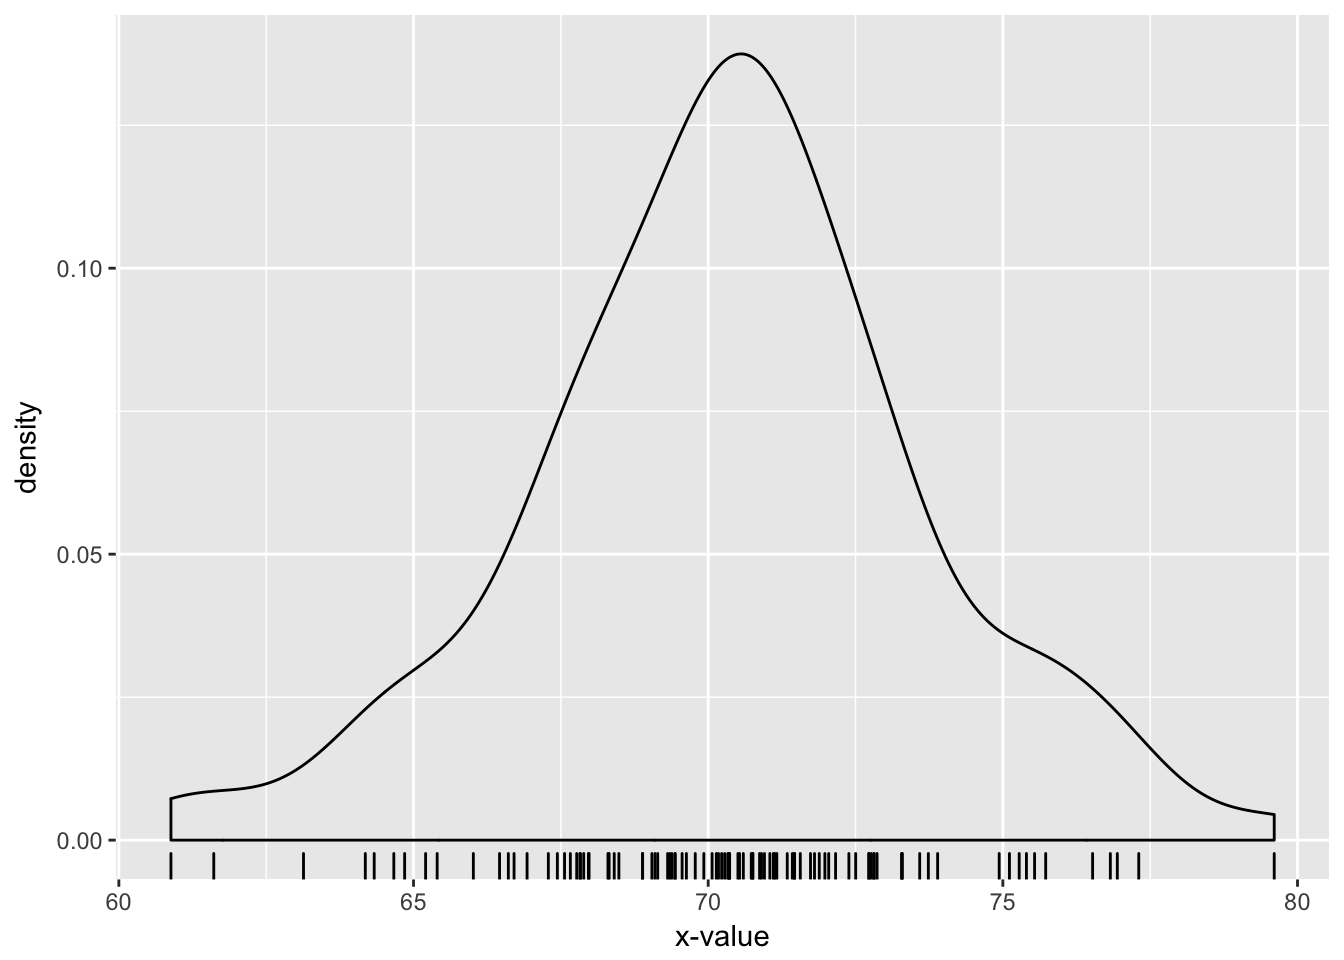
\includegraphics[width=0.6\linewidth]{r-notes_files/figure-latex/densitynormal-1} 

}

\caption{Density plot of 100 random values from a normal distribution with mean 70 and standard deviation 3.}\label{fig:densitynormal}
\end{figure}

The \texttt{geom\_density()} part of the plotting-command produces the
curve. The \texttt{geom\_rug()} part produces tick-marks along the
horizontal axis, each of which is located at a particular value in the
vector \texttt{x}. You can see that the curve is higher where values are
crowded together, and lower where the values are spread apart. The scale
on the y-axis has been chosen carefully so that the area under the
density curve between any two numbers \(a\) and \(b\) on the axis gives
an estimate of the chance that the normal random variable would produce
a value between \(a\) and \(b\). In this way the density curve gives us
a visual sense of the distribution of the random variable: it seems
rather likely to be between 67 and 73 (most of the area under the curve
occurs there) and rather unlikely to be greater than 76, and so on.

We are now ready to simulate the dental-floss scenario. Since we have
worked through the encapsulation-and-generalization development process
a number of times by now, we will simply show a final-form
implementation of a simulation function:

\begin{Shaded}
\begin{Highlighting}[]
\NormalTok{flossSim <-}\StringTok{ }\NormalTok{function(}\DataTypeTok{len =} \DecValTok{150}\NormalTok{, }\DataTypeTok{min =} \DecValTok{1}\NormalTok{, }
                     \DataTypeTok{max =} \DecValTok{2}\NormalTok{, }\DataTypeTok{reps =} \DecValTok{10000}\NormalTok{, }
                     \DataTypeTok{graph =} \OtherTok{FALSE}\NormalTok{, }\DataTypeTok{seed =} \OtherTok{NULL}\NormalTok{) \{}
  \NormalTok{if ( }\KeywordTok{is.null}\NormalTok{(seed) ) \{}
    \NormalTok{seed <-}\StringTok{ }\KeywordTok{as.numeric}\NormalTok{(}\KeywordTok{Sys.time}\NormalTok{())}
  \NormalTok{\}}
  \KeywordTok{set.seed}\NormalTok{(seed)}
  
  \CommentTok{# helper function to pick whihc box gets used:}
  \NormalTok{whichOne <-}\StringTok{ }\NormalTok{function(x) \{}
    \NormalTok{if (x <}\StringTok{ }\FloatTok{0.5} \NormalTok{) \{}
      \KeywordTok{return}\NormalTok{(}\StringTok{"a"}\NormalTok{)}
    \NormalTok{\} else }\KeywordTok{return}\NormalTok{(}\StringTok{"b"}\NormalTok{)}
  \NormalTok{\}}
  
  \CommentTok{# vector to contains our results:}
  \NormalTok{leftover <-}\StringTok{ }\KeywordTok{numeric}\NormalTok{(reps)}
  
  \CommentTok{# now the simulation.  Each time we loop through, we}
  \CommentTok{# start with two fresh boxes and use them until one of}
  \CommentTok{# them runs out.}
  \NormalTok{for (i in }\DecValTok{1}\NormalTok{:reps ) \{}
    \CommentTok{# set the initial lengh of the two fresh boxes:}
    \NormalTok{a <-}\StringTok{ }\NormalTok{b <-}\StringTok{ }\NormalTok{len}
    
    \CommentTok{# at the beignning, both can be used:}
    \NormalTok{bothOK <-}\StringTok{ }\OtherTok{TRUE}
    
    \CommentTok{# start flossing}
    \NormalTok{while ( bothOK ) \{}
      \CommentTok{# determine which box is picked}
      \CommentTok{# < 0.5 is a; >= 0.5 is b;}
      \NormalTok{boxPicked <-}\StringTok{ }\KeywordTok{whichOne}\NormalTok{(}\KeywordTok{runif}\NormalTok{(}\DecValTok{1}\NormalTok{))}
      
      \CommentTok{# if we choose box a, attempt to use floss from it}
      \NormalTok{if ( boxPicked ==}\StringTok{ "a"} \NormalTok{) \{}
        \NormalTok{if ( a <}\StringTok{ }\DecValTok{1} \NormalTok{) \{}
          \NormalTok{leftover[i] <-}\StringTok{ }\NormalTok{b}
          \NormalTok{bothOK <-}\StringTok{ }\OtherTok{FALSE}
        \NormalTok{\} else \{}
          \NormalTok{useAmount <-}\StringTok{ }\KeywordTok{min}\NormalTok{(}\KeywordTok{runif}\NormalTok{(}\DecValTok{1}\NormalTok{, min, max), a)}
          \NormalTok{a <-}\StringTok{ }\NormalTok{a -}\StringTok{ }\NormalTok{useAmount}
          \NormalTok{if (}\KeywordTok{abs}\NormalTok{(a) <}\StringTok{ }\DecValTok{10}\NormalTok{^(-}\DecValTok{4}\NormalTok{)) \{}
            \NormalTok{leftover[i] <-}\StringTok{ }\NormalTok{b}
            \NormalTok{bothOK <-}\StringTok{ }\OtherTok{FALSE}
          \NormalTok{\}}
        \NormalTok{\}}
      \NormalTok{\}}
      
      \CommentTok{# use floss from b (if we choose it) }
      \NormalTok{if ( boxPicked ==}\StringTok{ "b"} \NormalTok{) \{}
        \NormalTok{if ( b <}\StringTok{ }\DecValTok{1} \NormalTok{) \{}
          \NormalTok{leftover[i] <-}\StringTok{ }\NormalTok{a}
          \NormalTok{bothOK <-}\StringTok{ }\OtherTok{FALSE}
        \NormalTok{\} else \{}
          \NormalTok{useAmount <-}\StringTok{ }\KeywordTok{min}\NormalTok{(}\KeywordTok{runif}\NormalTok{(}\DecValTok{1}\NormalTok{, min, max), b)}
          \NormalTok{b <-}\StringTok{ }\NormalTok{b -}\StringTok{ }\NormalTok{useAmount}
          \NormalTok{if (}\KeywordTok{abs}\NormalTok{(b) <}\StringTok{ }\DecValTok{10}\NormalTok{^(-}\DecValTok{4}\NormalTok{)) \{}
            \NormalTok{leftover[i] <-}\StringTok{ }\NormalTok{a}
            \NormalTok{bothOK <-}\StringTok{ }\OtherTok{FALSE}
          \NormalTok{\}}
        \NormalTok{\}}
      \NormalTok{\}}
        
    \NormalTok{\}  }\CommentTok{# end while  loop}
  \NormalTok{\}    }\CommentTok{# end for loop}
  
  \CommentTok{# report results:}
  \NormalTok{if ( graph ) \{}
    \NormalTok{plotTitle <-}\StringTok{ }\KeywordTok{paste0}\NormalTok{(}\StringTok{"Dental-Floss Simulation with "}\NormalTok{, reps, }\StringTok{" Repetitions"}\NormalTok{)}
    \NormalTok{p <-}\StringTok{ }\KeywordTok{ggplot}\NormalTok{(}\DataTypeTok{mapping =} \KeywordTok{aes}\NormalTok{(leftover)) +}\StringTok{ }\KeywordTok{geom_density}\NormalTok{() +}
\StringTok{      }\KeywordTok{labs}\NormalTok{(}\DataTypeTok{x =} \StringTok{"Amount left in spare (ft)"}\NormalTok{,}
          \DataTypeTok{title =} \NormalTok{plotTitle)}
    \CommentTok{# add a rug of individual points, provided there are not too many:}
    \NormalTok{if ( reps <=}\StringTok{ }\DecValTok{100} \NormalTok{) \{}
      \NormalTok{p <-}\StringTok{ }\NormalTok{p +}\StringTok{ }\KeywordTok{geom_rug}\NormalTok{()}
    \NormalTok{\}}
  \NormalTok{\}}
  \KeywordTok{print}\NormalTok{(p)}
  \KeywordTok{cat}\NormalTok{(}\StringTok{"The average amount left in the spare is:  "}\NormalTok{, }
      \KeywordTok{mean}\NormalTok{(leftover), }\StringTok{"."}\NormalTok{, }\DataTypeTok{sep =} \StringTok{""}\NormalTok{)}
\NormalTok{\}      }\CommentTok{# end flossSim}
\end{Highlighting}
\end{Shaded}

Let's give it a try with 10,000 repetitions.

\begin{Shaded}
\begin{Highlighting}[]
\KeywordTok{flossSim}\NormalTok{(}\DataTypeTok{reps =} \DecValTok{10000}\NormalTok{, }\DataTypeTok{graph =} \OtherTok{TRUE}\NormalTok{, }\DataTypeTok{seed =} \DecValTok{3535}\NormalTok{)}
\end{Highlighting}
\end{Shaded}

\begin{figure}

{\centering 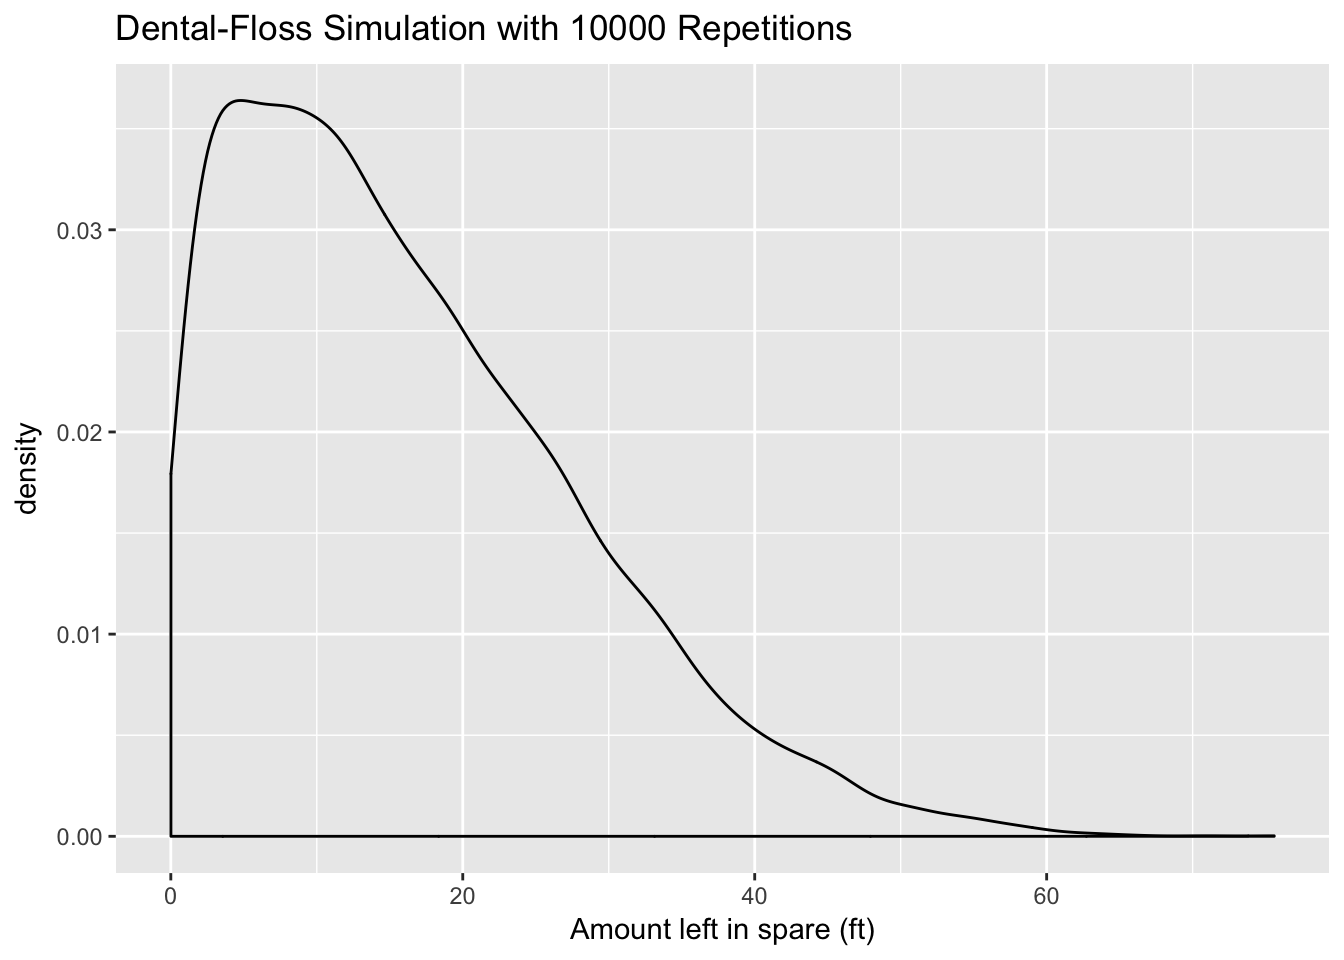
\includegraphics[width=0.6\linewidth]{r-notes_files/figure-latex/dentalflosssim-1} 

}

\caption{Density plot of the results of a dental-floss simulation.}\label{fig:dentalflosssim}
\end{figure}

\begin{verbatim}
## The average amount left in the spare is:  16.30542.
\end{verbatim}

A density plot of the results appears as Figure
\ref{fig:dentalflosssim}. The expected value of the amount left in the
remaining box is about 16.3 feet, but you can see from the plot that
there is quite a bit of variability: it's not all that unlikely to have
40 or more feet left!

\section{Example: The Drunken Turtle}\label{drunken-turtle-sim}

Let us return to the scenario of the Drunken Turtle that was introduced
in Section \ref{drunken-turtle-intro}. At each step the turtle would
turn by a random angle---any angle between 0 and 360 degrees with equal
likelihood---and then move forward by a fixed number of units. We
wondered whether the turtle would simply wander away from its starting
point or perhaps eventually loop back close to its starting point.

In this section we will construct a simulation that sheds light on our
question. We will imagine that the turtle starts at the origin on the
\(xy\)-plane and takes a large but fixed number of steps---one thousand
steps, say---each of a fixed length of one unit, but each of which is
preceded by a drunken turn through a random angle. We will concern
ourselves with the random variable \(X\), defined as follows:

\begin{quote}
\(X\) = the number of times in the turtle returns to within \(1/2\) of a
unit of the origin, during its first 1000 steps.
\end{quote}

(Apparently we consider a ``close return'' to be anything within half a
unit of the origin.)

In particular, we would like to know the distribution of \(X\): what is
the chance that the turtle does not make a close return during the first
thousand steps? What's the chance of making only one close return? Two
close returns? And so on \ldots{} . We would also like to estimate the
expected value of \(X\): the average number of close returns in the
first 1000 steps.

We will next consider how to code a simulation. Obviously we will need a
way to record the turtle's position at each step. In order to accomplish
this we will have to apply the unit-circle trigonometry you learned in
high school.

Instead of measuring angles in degrees, we will work in radians: by
default R does trigonometry that way. Recall that 360 degrees is
\(2 \pi\) radians; hence the way to determine the angle of a turn by the
drunken turtle is with the following call to \texttt{runif()}:

\begin{Shaded}
\begin{Highlighting}[]
\KeywordTok{runif}\NormalTok{(}\DecValTok{1}\NormalTok{, }\DataTypeTok{min =} \DecValTok{0}\NormalTok{, }\DataTypeTok{max =} \DecValTok{2}\NormalTok{*pi)}
\end{Highlighting}
\end{Shaded}

\begin{verbatim}
## [1] 2.746987
\end{verbatim}

If we want a thousand drunken turn-angles, then we can get them all in a
vector, as follows:

\begin{Shaded}
\begin{Highlighting}[]
\KeywordTok{runif}\NormalTok{(}\DecValTok{1000}\NormalTok{, }\DataTypeTok{min =} \DecValTok{0}\NormalTok{, }\DataTypeTok{max =} \DecValTok{2}\NormalTok{*pi)}
\end{Highlighting}
\end{Shaded}

So much for the turning angles. But in order to decide at each step
whether the turtle has made a close return, we have to know the
coordinates of the turtle after each step. This is where unit-circle
trigonometry comes in handy. Recall that if a right triangle has a
hypotenuse of length 1 (the length of a turtle step) and if one of the
angles of the triangle is \(\alpha\), then the side adjacent to
\(\alpha\) is \(\cos(\alpha)\) and the side opposite is
\(\sin(\alpha)\). The situation is illustrated in Figure
\ref{fig:right-triangle}.

\begin{figure}

{\centering 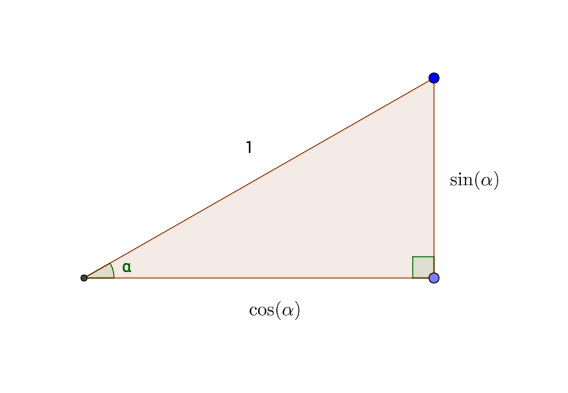
\includegraphics[width=0.75\linewidth]{images/righttriangle} 

}

\caption{Sides of a right triangle with hypotenuse 1, in terms of the angle shown.}\label{fig:right-triangle}
\end{figure}

From this principle it follows that if the turtle turns a random angle
of \(a_1\) radians for its first step, then after it takes the one-unit
step it will be at the point \((\cos(a_1), \sin(a_2))\).

For the second step, the turtle begins by turning another random angle,
say \(a_2\) radians. It then takes another one-unit step. This second
step forms the hypotenuse of a second right triangle (see Figure
\ref{fig:two-steps}). The horizontal and vertical sides of this right
triangle must be \(\cos(a_2)\) and \(\sin(a_2)\) respectively. When the
turtle complete the second step, it has added these values to its
previous \(x\) and \(y\) coordinates, so that it is now at the point:

\[(\cos(a_1) + \cos(a_2), \sin(a_1) +\sin(a_2)).\] We now see the idea:
in order to record the position of the turtle at the end of each step,
we simply need to:

\begin{itemize}
\tightlist
\item
  take the cosine of all the turning-angles;
\item
  take the sine of all the turning-angles;
\item
  sum the cosines to get the \(x\)-coordinate;
\item
  sum the sines to get the \(y\)-coordinate.
\end{itemize}

\begin{figure}

{\centering 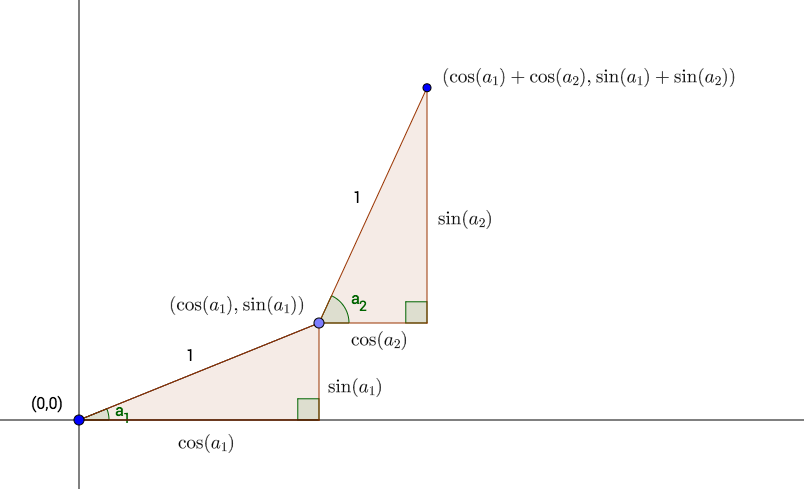
\includegraphics[width=0.75\linewidth]{images/twosteps} 

}

\caption{The first two steps by the Drunken Turtle.  Turtle turns by $a_1$ radians for Step One, then by $a_2$ radians for Step Two.}\label{fig:two-steps}
\end{figure}

Let's put this idea into practice, for just the first ten steps. First,
get the turning angles, the sines and the cosines:

\begin{Shaded}
\begin{Highlighting}[]
\NormalTok{angle <-}\StringTok{ }\KeywordTok{runif}\NormalTok{(}\DecValTok{10}\NormalTok{, }\DecValTok{0} \NormalTok{, }\DecValTok{2}\NormalTok{*pi)}
\NormalTok{xSteps <-}\StringTok{ }\KeywordTok{cos}\NormalTok{(angle)}
\NormalTok{ySteps <-}\StringTok{ }\KeywordTok{sin}\NormalTok{(angle)}
\end{Highlighting}
\end{Shaded}

Next, we need to add the \texttt{xSteps} together. If we do a sum, we
would get the \(x\)-coordinate after the tenth step:

\begin{Shaded}
\begin{Highlighting}[]
\KeywordTok{sum}\NormalTok{(xSteps)}
\end{Highlighting}
\end{Shaded}

\begin{verbatim}
## [1] -1.370258
\end{verbatim}

(Apparently some of the cosines were negative, meaning that some of the
turning angles were between 90 and 270 degrees.)

We need the \(x\)-coordinates after all of the previous steps, as well.
This can be accomplished by R's \texttt{cumsum()} function.
\index{R-functions!cumsum()@\texttt{cumsum()}} You may think of
\texttt{cumsum} as short for ``cumulative sum''. Given a vector
\texttt{vec} of numbers, \texttt{cumsum(vec)} returns a vector of the
same length, where for every index \texttt{i},
\texttt{cumsum(vec){[}i{]}} is \texttt{sum(vec{[}1:i{]})}. This is made
clear in the following example:

\begin{Shaded}
\begin{Highlighting}[]
\NormalTok{vec <-}\StringTok{ }\KeywordTok{c}\NormalTok{(}\DecValTok{1}\NormalTok{, }\DecValTok{1}\NormalTok{, }\DecValTok{1}\NormalTok{, }\DecValTok{1}\NormalTok{, }\DecValTok{1}\NormalTok{)}
\KeywordTok{cumsum}\NormalTok{(vec)}
\end{Highlighting}
\end{Shaded}

\begin{verbatim}
## [1] 1 2 3 4 5
\end{verbatim}

Accordingly, we can get the \(x\)-coordinates of the first ten steps
like this:

\begin{Shaded}
\begin{Highlighting}[]
\NormalTok{x <-}\StringTok{ }\KeywordTok{cumsum}\NormalTok{(xSteps)}
\NormalTok{x}
\end{Highlighting}
\end{Shaded}

\begin{verbatim}
##  [1] -0.6034165 -1.3905805 -2.1259607 -3.1154380 -2.4593130 -1.5476110
##  [7] -0.8591924 -1.6420445 -0.6421761 -1.3702583
\end{verbatim}

Similarly we can get the first ten \(y\)-coordinates:

\begin{Shaded}
\begin{Highlighting}[]
\NormalTok{y <-}\StringTok{ }\KeywordTok{cumsum}\NormalTok{(ySteps)}
\end{Highlighting}
\end{Shaded}

Using the distance formula, we can compute the distance of each point
from the origin as follows:

\begin{Shaded}
\begin{Highlighting}[]
\NormalTok{dist <-}\StringTok{ }\KeywordTok{sqrt}\NormalTok{(x^}\DecValTok{2} \NormalTok{+}\StringTok{ }\NormalTok{y^}\DecValTok{2}\NormalTok{)}
\end{Highlighting}
\end{Shaded}

The following logical vector will then record, at each each step,
whether or not the turtle has made a close return:

\begin{Shaded}
\begin{Highlighting}[]
\NormalTok{closeReturn <-}\StringTok{ }\NormalTok{(dist <}\StringTok{ }\FloatTok{0.5}\NormalTok{)}
\end{Highlighting}
\end{Shaded}

The results are shown in Table \ref{tab:tensteptab}.

\begin{table}

\caption{\label{tab:tensteptab}Record of the turtle's first ten steps.  It has not yet made a close return.}
\centering
\begin{tabular}[t]{r|r|r|r|r|r|l}
\hline
angle & xSteps & ySteps & x & y & dist & closeReturn\\
\hline
4.0646104 & -0.6034165 & -0.7974262 & -0.6034165 & -0.7974262 & 1.000000 & FALSE\\
\hline
2.4769935 & -0.7871641 & 0.6167437 & -1.3905805 & -0.1806826 & 1.402270 & FALSE\\
\hline
3.8861615 & -0.7353801 & -0.6776548 & -2.1259607 & -0.8583374 & 2.292695 & FALSE\\
\hline
2.9963954 & -0.9894774 & 0.1446876 & -3.1154380 & -0.7136497 & 3.196131 & FALSE\\
\hline
0.8551238 & 0.6561251 & 0.7546522 & -2.4593130 & 0.0410024 & 2.459655 & FALSE\\
\hline
0.4233886 & 0.9117020 & 0.4108522 & -1.5476110 & 0.4518546 & 1.612226 & FALSE\\
\hline
0.8114898 & 0.6884186 & 0.7253136 & -0.8591924 & 1.1771682 & 1.457373 & FALSE\\
\hline
2.4700328 & -0.7828521 & 0.6222079 & -1.6420445 & 1.7993761 & 2.435993 & FALSE\\
\hline
0.0162276 & 0.9998683 & 0.0162269 & -0.6421761 & 1.8156030 & 1.925826 & FALSE\\
\hline
3.8968689 & -0.7280822 & -0.6854899 & -1.3702583 & 1.1301131 & 1.776165 & FALSE\\
\hline
\end{tabular}
\end{table}

It remains only to package our code into a simulation function. We will
allow the user to specify the fixed initial number of steps (it does not
have to be 1000), and also to determine what distance counts as a
``close return.''

\begin{Shaded}
\begin{Highlighting}[]
\NormalTok{drunkenSim <-}\StringTok{ }\NormalTok{function(}\DataTypeTok{steps =} \DecValTok{1000}\NormalTok{, }\DataTypeTok{reps =} \DecValTok{10000}\NormalTok{, }\DataTypeTok{close =} \FloatTok{0.5}\NormalTok{, }
                       \DataTypeTok{seed =} \OtherTok{NULL}\NormalTok{, }\DataTypeTok{table =} \OtherTok{FALSE}\NormalTok{) \{}
  \NormalTok{if ( }\KeywordTok{is.null}\NormalTok{(seed) ) \{}
    \NormalTok{seed <-}\StringTok{ }\KeywordTok{Sys.time}\NormalTok{()}
  \NormalTok{\}}
  \KeywordTok{set.seed}\NormalTok{(seed)}
  
  \CommentTok{# set up returns vedtor to store the number of }
  \CommentTok{# close returns in each repetition:}
  \NormalTok{returns <-}\StringTok{ }\KeywordTok{numeric}\NormalTok{(reps)}
  
  \NormalTok{for (i in }\DecValTok{1}\NormalTok{:reps) \{}
  \NormalTok{angle <-}\StringTok{ }\KeywordTok{runif}\NormalTok{(steps, }\DecValTok{0} \NormalTok{, }\DecValTok{2}\NormalTok{*pi)}
  \NormalTok{xSteps <-}\StringTok{ }\KeywordTok{cos}\NormalTok{(angle)}
  \NormalTok{ySteps <-}\StringTok{ }\KeywordTok{sin}\NormalTok{(angle)}
  
  \NormalTok{x <-}\StringTok{ }\KeywordTok{cumsum}\NormalTok{(xSteps)}
  \NormalTok{y <-}\StringTok{ }\KeywordTok{cumsum}\NormalTok{(ySteps)}
  
  \NormalTok{dist <-}\StringTok{ }\KeywordTok{sqrt}\NormalTok{(x^}\DecValTok{2} \NormalTok{+}\StringTok{ }\NormalTok{y^}\DecValTok{2}\NormalTok{)}
  \NormalTok{closeReturn <-}\StringTok{ }\NormalTok{(dist <}\StringTok{ }\FloatTok{0.5}\NormalTok{)}
  \NormalTok{returns[i] <-}\StringTok{ }\KeywordTok{sum}\NormalTok{(closeReturn)}
  \NormalTok{\}}
  
  \NormalTok{if ( table ) \{}
    \KeywordTok{cat}\NormalTok{(}\StringTok{"Here is a table of the number of close returns:}\CharTok{\textbackslash{}n\textbackslash{}n}\StringTok{"}\NormalTok{)}
    \NormalTok{tab <-}\StringTok{ }\KeywordTok{prop.table}\NormalTok{(}\KeywordTok{table}\NormalTok{(returns))}
    \KeywordTok{print}\NormalTok{(tab)}
    \KeywordTok{cat}\NormalTok{(}\StringTok{"}\CharTok{\textbackslash{}n}\StringTok{"}\NormalTok{)}
  \NormalTok{\}}
  \KeywordTok{cat}\NormalTok{(}\StringTok{"The average number of close returns was:  "}\NormalTok{, }
      \KeywordTok{mean}\NormalTok{(returns), }\StringTok{"."}\NormalTok{, }\DataTypeTok{sep =} \StringTok{""}\NormalTok{)}
\NormalTok{\}}
\end{Highlighting}
\end{Shaded}

Let's try it out:

\begin{Shaded}
\begin{Highlighting}[]
\KeywordTok{drunkenSim}\NormalTok{(}\DataTypeTok{steps =} \DecValTok{1000}\NormalTok{, }\DataTypeTok{reps =} \DecValTok{10000}\NormalTok{, }
           \DataTypeTok{close =} \FloatTok{0.5}\NormalTok{, }\DataTypeTok{seed =} \DecValTok{3535}\NormalTok{, }\DataTypeTok{table =} \OtherTok{TRUE}\NormalTok{)}
\end{Highlighting}
\end{Shaded}

\begin{verbatim}
## Here is a table of the number of close returns:
## 
## returns
##      0      1      2      3      4      5      6      7      8      9 
## 0.3881 0.2290 0.1517 0.0908 0.0572 0.0335 0.0227 0.0107 0.0064 0.0048 
##     10     11     12     13     14     15     16     17 
## 0.0018 0.0012 0.0008 0.0007 0.0003 0.0001 0.0001 0.0001 
## 
## The average number of close returns was:  1.5655.
\end{verbatim}

Notice that 38.81\% of the time the turtle did not make a close return
at all during the first thousand steps. On the other hand it is
possible, though not at all likely, for the turtle to make quite a few
close returns.\footnote{Note that these proportions depend heavily on
  how we define ``close''. If the cut-off had been lower than \(1/2\),
  then we would have seen fewer close returns.}

It is interesting to look specifically at the distances from the origin.
The following function draws a graph of the distance from the origin for
the specified number of turtle steps:

\begin{Shaded}
\begin{Highlighting}[]
\NormalTok{drunkenSim2 <-}\StringTok{ }\NormalTok{function(}\DataTypeTok{steps =} \DecValTok{1000}\NormalTok{, }\DataTypeTok{seed =} \OtherTok{NULL}\NormalTok{) \{}
  \NormalTok{if ( }\KeywordTok{is.null}\NormalTok{(seed) ) \{}
    \NormalTok{seed <-}\StringTok{ }\KeywordTok{Sys.time}\NormalTok{()}
  \NormalTok{\}}
  \KeywordTok{set.seed}\NormalTok{(seed)}
  
  \NormalTok{angle <-}\StringTok{ }\KeywordTok{runif}\NormalTok{(steps, }\DecValTok{0} \NormalTok{, }\DecValTok{2}\NormalTok{*pi)}
  \NormalTok{xSteps <-}\StringTok{ }\KeywordTok{cos}\NormalTok{(angle)}
  \NormalTok{ySteps <-}\StringTok{ }\KeywordTok{sin}\NormalTok{(angle)}
  \NormalTok{x <-}\StringTok{ }\KeywordTok{cumsum}\NormalTok{(xSteps)}
  \NormalTok{y <-}\StringTok{ }\KeywordTok{cumsum}\NormalTok{(ySteps)}
  \NormalTok{dist <-}\StringTok{ }\KeywordTok{sqrt}\NormalTok{(x^}\DecValTok{2} \NormalTok{+}\StringTok{ }\NormalTok{y^}\DecValTok{2}\NormalTok{)}
  \NormalTok{plotTitle <-}\StringTok{ }\KeywordTok{paste0}\NormalTok{(}\StringTok{"First "}\NormalTok{, steps, }\StringTok{" Steps of the Drunken Turtle"}\NormalTok{)}
  \NormalTok{p <-}\StringTok{ }\KeywordTok{ggplot}\NormalTok{(}\DataTypeTok{mapping =} \KeywordTok{aes}\NormalTok{(}\DataTypeTok{x =} \DecValTok{1}\NormalTok{:steps, }\DataTypeTok{y=}\NormalTok{dist)) +}\StringTok{ }\KeywordTok{geom_line}\NormalTok{() +}
\StringTok{    }\KeywordTok{labs}\NormalTok{(}\DataTypeTok{x =} \StringTok{"Step"}\NormalTok{, }\DataTypeTok{y =} \StringTok{"Distance From Origin"}\NormalTok{,}
         \DataTypeTok{title =} \NormalTok{plotTitle)}
  \KeywordTok{print}\NormalTok{(p)}
\NormalTok{\}}
\end{Highlighting}
\end{Shaded}

Let's try it out! The results appear in Figure
\ref{fig:drunken-turtle-steps}

\begin{Shaded}
\begin{Highlighting}[]
\KeywordTok{drunkenSim2}\NormalTok{(}\DataTypeTok{steps =} \DecValTok{1000}\NormalTok{, }\DataTypeTok{seed =} \DecValTok{2525}\NormalTok{)}
\end{Highlighting}
\end{Shaded}

\begin{figure}

{\centering 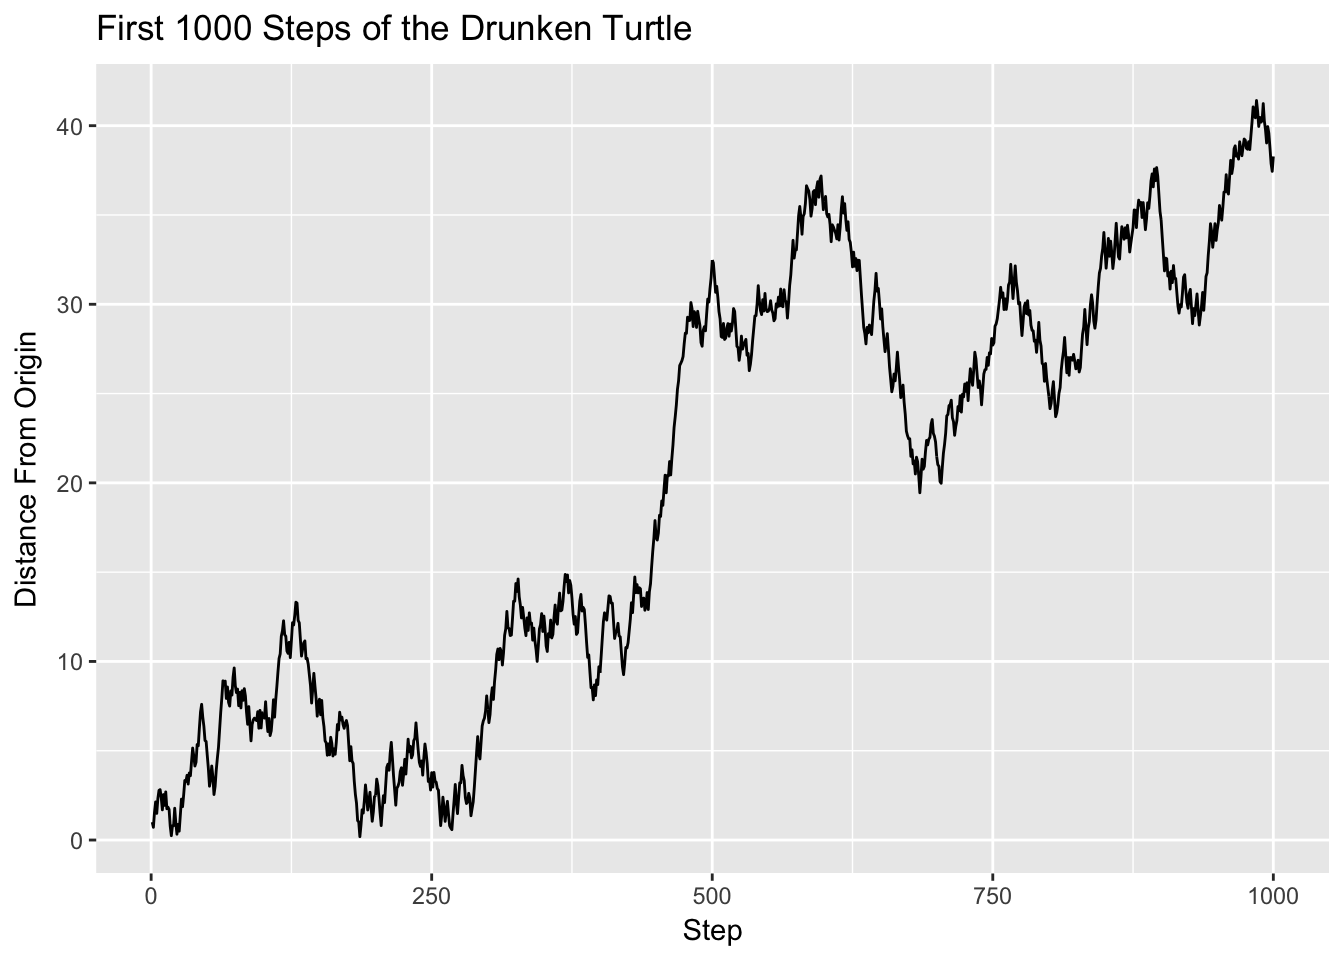
\includegraphics[width=0.6\linewidth]{r-notes_files/figure-latex/drunken-turtle-steps-1} 

}

\caption{Line plot of the Turtle's distance from the origin, as a function of how many steps the turtle has taken.}\label{fig:drunken-turtle-steps}
\end{figure}

It appears that although the turtle might have returned close to the
origin a couple of times, for the most part it seems to be wandering
further and further away. In the mathematical field known as
\emph{stochastic processes}, it has been shown that if the turtle is
allowed to go on forever then it will certainly make a close return
\emph{infinitely many times}. These returns, though, will tend to be
spaced further and further apart as time goes on, and our graph suggests
that this is so.

\newpage

\section*{Glossary}\label{glossary-4}
\addcontentsline{toc}{section}{Glossary}

\begin{description}
\item[Probability of an Event \index{probability}]
The long-run proportion of times that the event will occur if the
underlying random process is repeated many, many times.
\item[Random Variable \index{random variable}]
A number whose value depends on the outcome of a chance process.
\item[Expected Value of a Random Variable \index{expected value}]
The long-run average of the values of a random variable, where the
underlying chance process is repeated many, many times.
\item[Continuous Random Variable \index{continuous random variable}]
A random variable that can assume any value in a range of real numbers.
\item[Distribution of a Random Variable \index{distribution}]
A statement of the probabilities for a random variable to assume its
various possible values.
\item[Encapsulation and Generalization
\index{encapsulation and generalization}]
A method for developing a computer program according to which the
programmer first designs a basic procedure, then encapsulates it in one
or more functions, and then progressively generalizes these functions
until the program possesses all desired features.
\end{description}

\newpage

\section*{Exercises}\label{exercises-4}
\addcontentsline{toc}{section}{Exercises}

\begin{center}
\includegraphics[width=0.5\linewidth]{images/thinking} \end{center}

\begin{enumerate}
\def\labelenumi{\arabic{enumi}.}
\item
  Consider the following two games.

  \begin{itemize}
  \tightlist
  \item
    In Game A you flip a fair coin. If the coin comes up Heads you get
    two dollars, whereas if it comes up Tails you get one dollar.
  \item
    In Game B you roll a fair die. If the six-spot comes up, you win
    twenty-five dollars. If you get 3, 4, or 5, nothing happens. If the
    one-spot comes up, you lose fifteen dollars.
  \end{itemize}

  You can choose either to play Game A ten thousand times or to play
  Game B ten thousand times. You wonder: \emph{which game is the better
  choice?} Before you answer the question, write two simulation
  functions: one that provides an estimate of the expected value of the
  winnings from a play of Game A, and another that estimates the
  expected value of the winnings from a play of Game B. The functions
  should have two parameters:

  \begin{itemize}
  \tightlist
  \item
    a \texttt{rep} parameter to permit the user to choose the number of
    repetitions of the game;
  \item
    a \texttt{seed} parameter to permit the user to choose a starting
    seed.
  \end{itemize}

  Try both functions with ten thousand reps and with simple starting
  seeds. Report the seeds you used for each function, and the estimated
  expected values for each game. Use your results to decide which game
  is the better choice.
\item
  Reconsider the meeting of Anna and Raj. Suppose that they still plan
  to meet during the same one-hour period, but that Anna is willing to
  wait \(a\) minutes and Raj is willing to wait \(r\) minutes, where
  \(a\) and \(r\) could differ. Modify the \texttt{meetupSim()} function
  so that it accepts two additional parameters:

  \begin{itemize}
  \tightlist
  \item
    \texttt{a}: the time Anna is willing to wait;
  \item
    \texttt{r}: the time Raj is willing to wait;
  \end{itemize}

  Apply the function with ten thousand repetitions (and a simple seed
  that you report) in order to estimate the probability of a meeting,
  assuming that Anna is willing to wait 13 minutes and Raj is willing to
  wait 7 minutes.
\item
  A pipe-smoker has two boxes of matches in his pocket. Both boxes
  contain 40 matches. Every time he lights his pipe, the smoker reaches
  into his pocket and randomly picks one of the boxes, pulling a match
  from the box. Eventually one of the boxes runs out. What is the
  expected value of the number of matches remaining in the other box at
  that time? Write a simulation function to estimate the answer. Your
  function should have at least a \texttt{reps} and a \texttt{seed}
  parameter. Apply the function with ten thousand repetitions---and with
  a simple seed that you report---in order to estimate the expected
  value.
\item
  Refer back to the \texttt{numberNeededSim()} function. Modify it so
  that it returns the estimated expected value invisibly, and has an
  option to turn off the \texttt{cat()} report to the console. Write a
  program that computes the estimated expected number needed, for the
  following targets:

\begin{Shaded}
\begin{Highlighting}[]
\NormalTok{targets <-}\StringTok{ }\KeywordTok{seq}\NormalTok{(}\FloatTok{0.05}\NormalTok{, }\FloatTok{0.95}\NormalTok{, }\DataTypeTok{by =} \FloatTok{0.05}\NormalTok{)}
\end{Highlighting}
\end{Shaded}

  Each estimate should be based on ten thousand repetitions. Start with
  a simple seed that you report. Report the estimated expected values
  for all of the required targets. Compare these estimates with
  \texttt{exp(targets)} (the number \(e\) raised to the power of each of
  the targets.) Formulate a conjecture about the value of the expected
  number of numbers needed, when the target is a real number between 0
  and 1.
\item
  A gambler starts with 10 dollars, and repeatedly plays a game. If she
  wins the game he gets one dollar and if she loses the game he
  losesonea dollar. She has a 45 percent chance of winning the game.
  Write a function to simulate the gambler repeatedly playing the game
  until her money runs out. The function should keep track of how much
  money she has left after each play, so that it can produce a line
  graph (similar to the one in the section on the Drunken Turtle) of the
  money left after each play. Write the function so that it has

  \begin{itemize}
  \tightlist
  \item
    a \texttt{start} parameter for the initial amount of money the
    gambler has;
  \item
    a \texttt{seed} parameter`
  \item
    a \texttt{p} parameter for the chance of winning, so that the user
    can enter any chance less than or equal to 0.5. (The function should
    stop the user if the user enters more than 0.5.)
  \end{itemize}

  Apply the function with a simple seed that you report, a starting
  amount of ten dollars, and a chance of winning equal to 0.45.
\end{enumerate}

\chapter{Data Frames}\label{frames}

\BeginKnitrBlock{leadquote}
\emph{Can one be a good data analyst without being a half-good
programmer? The short answer to that is, `No.' The long answer to that
is, `No.'}

---Frank Harrell
\EndKnitrBlock{leadquote}

Up to this point we have given a great deal of attention to vectors, and
we have always treated them as one-dimensional objects: a vector has a
length, but not a ``width.''

It is time to begin working in two dimensions. In this Chapter we will
study \emph{matrices}, which are simply vectors that have both length
and width. Matrices are immensely useful for scientific computation in
R, but for the most part we will treat them as a warm-up for \emph{data
frames}---the two-dimensional R-objects that are especially designed for
the storage of data collected in the course of practical data analysis.
Once you understand how to construct and manipulate data frames, you
will be ready to learn how to visualize and analyze data using R.

\newpage

\section{Introduction to Matrices}\label{introduction-to-matrices}

In R, a \emph{matrix} \index{matrix} is actually an atomic vector---it
can only hold one type of element---but with two extra attributes:

\begin{itemize}
\tightlist
\item
  a certain number of rows, and
\item
  a certain number of columns.
\end{itemize}

One way to create is matrix is to take a vector and \emph{give} it those
two extra attributes, via the \texttt{matrix()} function.
\index{R-functions!matrix()@\texttt{matrix()}} Here is an example:

\begin{Shaded}
\begin{Highlighting}[]
\NormalTok{numbers <-}\StringTok{ }\DecValTok{1}\NormalTok{:}\DecValTok{24}  \CommentTok{# this is an ordinary atomic vector}
\NormalTok{numbersMat <-}\StringTok{ }\KeywordTok{matrix}\NormalTok{(numbers, }\DataTypeTok{nrow =} \DecValTok{6}\NormalTok{, }\DataTypeTok{ncol =} \DecValTok{4}\NormalTok{)  }\CommentTok{# make a matrix}
\NormalTok{numbersMat}
\end{Highlighting}
\end{Shaded}

\begin{verbatim}
##      [,1] [,2] [,3] [,4]
## [1,]    1    7   13   19
## [2,]    2    8   14   20
## [3,]    3    9   15   21
## [4,]    4   10   16   22
## [5,]    5   11   17   23
## [6,]    6   12   18   24
\end{verbatim}

Of course if you are making a matrix out of 24 numbers and you know that
it's going to have 6 rows, then you know it must have 4 columns.
Similarly, if you know the number of columns then the number of rows is
determined. Hence you could have just as well constructed the matrix
with just one of the row or column arguments, like this:

\begin{Shaded}
\begin{Highlighting}[]
\NormalTok{numbersMat <-}\StringTok{ }\KeywordTok{matrix}\NormalTok{(numbers, }\DataTypeTok{nrow =} \DecValTok{6}\NormalTok{)}
\end{Highlighting}
\end{Shaded}

Notice that the numbers went down the first column, then down the
second, and so on. If you would rather fill up the matrix row-by-row,
then set the \texttt{byrow} parameter, which is \texttt{FALSE} by
default, to \texttt{TRUE}:

\begin{Shaded}
\begin{Highlighting}[]
\KeywordTok{matrix}\NormalTok{(numbers, }\DataTypeTok{nrow =} \DecValTok{6}\NormalTok{, }\DataTypeTok{byrow =} \OtherTok{TRUE}\NormalTok{)}
\end{Highlighting}
\end{Shaded}

\begin{verbatim}
##      [,1] [,2] [,3] [,4]
## [1,]    1    2    3    4
## [2,]    5    6    7    8
## [3,]    9   10   11   12
## [4,]   13   14   15   16
## [5,]   17   18   19   20
## [6,]   21   22   23   24
\end{verbatim}

Sometimes we like to give names to our rows, or to our columns, or even
to both:

\begin{Shaded}
\begin{Highlighting}[]
\KeywordTok{rownames}\NormalTok{(numbersMat) <-}\StringTok{ }\NormalTok{letters[}\DecValTok{1}\NormalTok{:}\DecValTok{6}\NormalTok{]}
\KeywordTok{colnames}\NormalTok{(numbersMat) <-}\StringTok{ }\NormalTok{LETTERS[}\DecValTok{1}\NormalTok{:}\DecValTok{4}\NormalTok{]}
\NormalTok{numbersMat}
\end{Highlighting}
\end{Shaded}

\begin{verbatim}
##   A  B  C  D
## a 1  7 13 19
## b 2  8 14 20
## c 3  9 15 21
## d 4 10 16 22
## e 5 11 17 23
## f 6 12 18 24
\end{verbatim}

Matrices don't have to be numerical. They can be character or logical
matrices as well:

\begin{Shaded}
\begin{Highlighting}[]
\NormalTok{creatures <-}\StringTok{ }\KeywordTok{c}\NormalTok{(}\StringTok{"Dorothy"}\NormalTok{, }\StringTok{"Lion"}\NormalTok{, }\StringTok{"Scarecrow"}\NormalTok{, }\StringTok{"Oz"}\NormalTok{,}
               \StringTok{"Toto"}\NormalTok{, }\StringTok{"Boq"}\NormalTok{)}
\KeywordTok{matrix}\NormalTok{(creatures, }\DataTypeTok{ncol =} \DecValTok{2}\NormalTok{)}
\end{Highlighting}
\end{Shaded}

\begin{verbatim}
##      [,1]        [,2]  
## [1,] "Dorothy"   "Oz"  
## [2,] "Lion"      "Toto"
## [3,] "Scarecrow" "Boq"
\end{verbatim}

If you have to spread out the elements of a matrix into a
one-dimensional vector, you can do so:

\begin{Shaded}
\begin{Highlighting}[]
\KeywordTok{as.vector}\NormalTok{(numbersMat)}
\end{Highlighting}
\end{Shaded}

\begin{verbatim}
##  [1]  1  2  3  4  5  6  7  8  9 10 11 12 13 14 15 16 17 18 19 20 21 22 23
## [24] 24
\end{verbatim}

\section{Matrix Indexing}\label{matrix-indexing}

Matrices are incredibly useful in data analysis, but the primary reason
we are talking about them now is to get you used to working in two
dimensions. Let's practice sub-setting with matrices.

We use the sub-setting operator \texttt{{[}} to pick out parts of a
matrix. For example, in order to get the element in the second row and
third column of \texttt{numbersMat}, ask for:

\begin{Shaded}
\begin{Highlighting}[]
\NormalTok{numbersMat[}\DecValTok{2}\NormalTok{,}\DecValTok{3}\NormalTok{]}
\end{Highlighting}
\end{Shaded}

\begin{verbatim}
## [1] 14
\end{verbatim}

The row and column numbers are called \emph{indices}.

If we want the entire second row, then we could ask for:

\begin{Shaded}
\begin{Highlighting}[]
\NormalTok{numbersMat[}\DecValTok{2}\NormalTok{,}\DecValTok{1}\NormalTok{:}\DecValTok{4}\NormalTok{]}
\end{Highlighting}
\end{Shaded}

\begin{verbatim}
##  A  B  C  D 
##  2  8 14 20
\end{verbatim}

The result is a one-dimensional vector consisting of the elements in the
second row of \texttt{numbersMat}. It inherits as its names the column
names of \texttt{numbersMat}.

Actually, if you want the entire row you don't have to specify which
columns you want. Just leave the spot after the comma empty, like this:

\begin{Shaded}
\begin{Highlighting}[]
\NormalTok{numbersMat[}\DecValTok{2}\NormalTok{, ]}
\end{Highlighting}
\end{Shaded}

\begin{verbatim}
##  A  B  C  D 
##  2  8 14 20
\end{verbatim}

What if you want some items on the second row, but only the items in
columns 1, 2 and 4? Then frame your request in terms of a vector of
column-indices:

\begin{Shaded}
\begin{Highlighting}[]
\NormalTok{numbersMat[}\DecValTok{2}\NormalTok{, }\KeywordTok{c}\NormalTok{(}\DecValTok{1}\NormalTok{, }\DecValTok{2}\NormalTok{, }\DecValTok{4}\NormalTok{)]}
\end{Highlighting}
\end{Shaded}

\begin{verbatim}
##  A  B  D 
##  2  8 20
\end{verbatim}

You can specify a vector of row-indices along with a vector of
column-indices, if you like:

\begin{Shaded}
\begin{Highlighting}[]
\NormalTok{numbersMat[}\DecValTok{1}\NormalTok{:}\DecValTok{2}\NormalTok{, }\DecValTok{1}\NormalTok{:}\DecValTok{3}\NormalTok{]}
\end{Highlighting}
\end{Shaded}

\begin{verbatim}
##   A B  C
## a 1 7 13
## b 2 8 14
\end{verbatim}

If the vector has row or column names then you may use them in place of
indices to make a selection:

\begin{Shaded}
\begin{Highlighting}[]
\NormalTok{numbersMat[, }\KeywordTok{c}\NormalTok{(}\StringTok{"B"}\NormalTok{, }\StringTok{"D"}\NormalTok{)]}
\end{Highlighting}
\end{Shaded}

\begin{verbatim}
##    B  D
## a  7 19
## b  8 20
## c  9 21
## d 10 22
## e 11 23
## f 12 24
\end{verbatim}

You can use sub-setting to change the values of the elements of a matrix

\begin{Shaded}
\begin{Highlighting}[]
\NormalTok{numbersMat[}\DecValTok{2}\NormalTok{,}\DecValTok{3}\NormalTok{] <-}\StringTok{ }\DecValTok{0}
\NormalTok{numbersMat}
\end{Highlighting}
\end{Shaded}

\begin{verbatim}
##   A  B  C  D
## a 1  7 13 19
## b 2  8  0 20
## c 3  9 15 21
## d 4 10 16 22
## e 5 11 17 23
## f 6 12 18 24
\end{verbatim}

You can assign a value to an entire row:

\begin{Shaded}
\begin{Highlighting}[]
\NormalTok{numbersMat[}\DecValTok{2}\NormalTok{,] <-}\StringTok{ }\DecValTok{0}
\NormalTok{numbersMat}
\end{Highlighting}
\end{Shaded}

\begin{verbatim}
##   A  B  C  D
## a 1  7 13 19
## b 0  0  0  0
## c 3  9 15 21
## d 4 10 16 22
## e 5 11 17 23
## f 6 12 18 24
\end{verbatim}

In the code above, the 0 was ``recycled'' \index{recycling} into each of
the four elements of the second row

You can assign the elements of a vector to corresponding selected
elements of a matrix:

\begin{Shaded}
\begin{Highlighting}[]
\NormalTok{numbersMat[}\DecValTok{2}\NormalTok{,] <-}\StringTok{ }\KeywordTok{c}\NormalTok{(}\DecValTok{100}\NormalTok{, }\DecValTok{200}\NormalTok{, }\DecValTok{300}\NormalTok{, }\DecValTok{400}\NormalTok{)}
\NormalTok{numbersMat}
\end{Highlighting}
\end{Shaded}

\begin{verbatim}
##     A   B   C   D
## a   1   7  13  19
## b 100 200 300 400
## c   3   9  15  21
## d   4  10  16  22
## e   5  11  17  23
## f   6  12  18  24
\end{verbatim}

\subsection{To Drop or Not?}\label{to-drop-or-not}

Note that when we ask for a single row of \texttt{numbersMat} we got a
regular one-dimensional vector:

\begin{Shaded}
\begin{Highlighting}[]
\NormalTok{numbersMat[}\DecValTok{3}\NormalTok{, ]}
\end{Highlighting}
\end{Shaded}

\begin{verbatim}
##  A  B  C  D 
##  3  9 15 21
\end{verbatim}

The same things happens if we ask for a single column:

\begin{Shaded}
\begin{Highlighting}[]
\NormalTok{numbersMat[ , }\DecValTok{2}\NormalTok{]}
\end{Highlighting}
\end{Shaded}

\begin{verbatim}
##   a   b   c   d   e   f 
##   7 200   9  10  11  12
\end{verbatim}

We get the second column of \texttt{numbersMat}, but as a regular
vector. It's not a ``column'' anymore. (Note that it inherits the row
names from \texttt{numbersMat}.)

When a subset of a matrix comes from only one row or column, R takes the
opportunity to ``drop'' the class of the subset from ``matrix'' to
``vector.'' If you would like the subset to stay a vector, set the
\texttt{drop} parameter, which by default is \texttt{TRUE}, to
\texttt{FALSE}. Thus the second column of \texttt{numbersMat}, kept as a
matrix with six rows and one column, is found as follows:

\begin{Shaded}
\begin{Highlighting}[]
\NormalTok{numbersMat[ , }\DecValTok{2}\NormalTok{, drop =}\StringTok{ }\OtherTok{FALSE}\NormalTok{]}
\end{Highlighting}
\end{Shaded}

\begin{verbatim}
##     B
## a   7
## b 200
## c   9
## d  10
## e  11
## f  12
\end{verbatim}

In most applications people want the simpler vector structure, so they
usually leave \texttt{drop} at its default value.

\section{Operations on Matrices}\label{operations-on-matrices}

Matrices can be involved in arithmetical and logical operations.

\subsection{Arithmetical Operations}\label{arithmetical-operations}

The usual arithmetic operations apply to matrices, operating
element-wise. For example, suppose that we have:

\begin{Shaded}
\begin{Highlighting}[]
\NormalTok{mat1 <-}\StringTok{ }\KeywordTok{matrix}\NormalTok{(}\KeywordTok{rep}\NormalTok{(}\DecValTok{1}\NormalTok{, }\DecValTok{4}\NormalTok{), }\DataTypeTok{nrow =} \DecValTok{2}\NormalTok{)}
\NormalTok{mat2 <-}\StringTok{ }\KeywordTok{matrix}\NormalTok{(}\KeywordTok{rep}\NormalTok{(}\DecValTok{2}\NormalTok{, }\DecValTok{4}\NormalTok{), }\DataTypeTok{nrow =} \DecValTok{2}\NormalTok{)}
\end{Highlighting}
\end{Shaded}

To get the sum of the above two matrices, R adds their corresponding
elements and forms a new matrix out of their sums, thus:

\begin{Shaded}
\begin{Highlighting}[]
\NormalTok{mat1 +}\StringTok{ }\NormalTok{mat2}
\end{Highlighting}
\end{Shaded}

\begin{verbatim}
##      [,1] [,2]
## [1,]    3    3
## [2,]    3    3
\end{verbatim}

R applies recycling as needed. For example, suppose we have:

\begin{Shaded}
\begin{Highlighting}[]
\NormalTok{mat <-}\StringTok{ }\KeywordTok{matrix}\NormalTok{(}\DecValTok{1}\NormalTok{:}\DecValTok{4}\NormalTok{, }\DataTypeTok{nrow =} \DecValTok{2}\NormalTok{)}
\NormalTok{mat}
\end{Highlighting}
\end{Shaded}

\begin{verbatim}
##      [,1] [,2]
## [1,]    1    3
## [2,]    2    4
\end{verbatim}

In order to multiply each element of \texttt{mat} by 2, we need not
create a 2-by-2 matrix of 2's. We can simply multiply by 2, and R will
take care of recycling the 2:

\begin{Shaded}
\begin{Highlighting}[]
\DecValTok{2} \NormalTok{*}\StringTok{ }\NormalTok{mat}
\end{Highlighting}
\end{Shaded}

\begin{verbatim}
##      [,1] [,2]
## [1,]    2    6
## [2,]    4    8
\end{verbatim}

Or we could subtract 3 from each element of \texttt{mat}:

\begin{Shaded}
\begin{Highlighting}[]
\NormalTok{mat -}\StringTok{ }\DecValTok{3}
\end{Highlighting}
\end{Shaded}

\begin{verbatim}
##      [,1] [,2]
## [1,]   -2    0
## [2,]   -1    1
\end{verbatim}

\subsection{Matrix Multiplication}\label{matrix-multiplication}

This section is optional reading, but it may interest you if you know
about matrix multiplication in linear algebra.

In order to accomplish matrix multiplication, we have to keep in mind
that the regular multiplication operator \texttt{*} works element-wise
on matrices, as we have already seen. For matrix multiplication R
provides the special operator \texttt{\%*\%}. For example, consider the
following matrices:

\begin{Shaded}
\begin{Highlighting}[]
\NormalTok{a <-}\StringTok{ }\KeywordTok{matrix}\NormalTok{(}\DecValTok{1}\NormalTok{:}\DecValTok{6}\NormalTok{, }\DataTypeTok{ncol =} \DecValTok{3}\NormalTok{)}
\NormalTok{a}
\end{Highlighting}
\end{Shaded}

\begin{verbatim}
##      [,1] [,2] [,3]
## [1,]    1    3    5
## [2,]    2    4    6
\end{verbatim}

\begin{Shaded}
\begin{Highlighting}[]
\NormalTok{b <-}\StringTok{ }\KeywordTok{matrix}\NormalTok{(}\KeywordTok{c}\NormalTok{(}\DecValTok{2}\NormalTok{, }\DecValTok{1}\NormalTok{, -}\DecValTok{1}\NormalTok{), }\DataTypeTok{nrow =} \DecValTok{3}\NormalTok{)}
\NormalTok{b}
\end{Highlighting}
\end{Shaded}

\begin{verbatim}
##      [,1]
## [1,]    2
## [2,]    1
## [3,]   -1
\end{verbatim}

Observe that the number of columns of \texttt{a} is equal to the number
of rows of \texttt{b}. Hence it is possible to form the matrix product
\texttt{a\ \%*\%\ b}:

\begin{Shaded}
\begin{Highlighting}[]
\NormalTok{a %*%}\StringTok{ }\NormalTok{b}
\end{Highlighting}
\end{Shaded}

\begin{verbatim}
##      [,1]
## [1,]    0
## [2,]    2
\end{verbatim}

As expected, the result is a matrix having as many rows as the rows of
\texttt{a}and as many columns as the columns of \texttt{b}.

It is also interesting to recall how matrix multiplication works when
the second matrix has only one column. The product is obtained by
multiplying each column of \texttt{a} by the element on the
corresponding row of \texttt{b}, and adding the resulting matrices:

\begin{Shaded}
\begin{Highlighting}[]
\NormalTok{b[}\DecValTok{1}\NormalTok{,}\DecValTok{1}\NormalTok{]*a[ ,}\DecValTok{1}\NormalTok{, drop =}\StringTok{ }\NormalTok{F] +}\StringTok{ }\NormalTok{b[}\DecValTok{2}\NormalTok{,}\DecValTok{1}\NormalTok{, drop =}\StringTok{ }\NormalTok{F]*a[ ,}\DecValTok{2}\NormalTok{] +}\StringTok{ }\NormalTok{b[}\DecValTok{3}\NormalTok{,}\DecValTok{1}\NormalTok{]*a[ ,}\DecValTok{3}\NormalTok{, drop =}\StringTok{ }\NormalTok{F]}
\end{Highlighting}
\end{Shaded}

\begin{verbatim}
##      [,1]
## [1,]    0
## [2,]    2
\end{verbatim}

\subsection{Logical Operations}\label{logical-operations}

Boolean operations apply to matrices element-wise, just as they do to
ordinary vectors. The result is a matrix of logical values. For
examples, consider the original matrix \texttt{numbersMat}:

\begin{Shaded}
\begin{Highlighting}[]
\NormalTok{numbersMat <-}\StringTok{ }\KeywordTok{matrix}\NormalTok{(}\DecValTok{1}\NormalTok{:}\DecValTok{24}\NormalTok{, }\DataTypeTok{nrow =} \DecValTok{6}\NormalTok{)}
\end{Highlighting}
\end{Shaded}

Suppose we wish to determine which elements of \texttt{numbersMat} are
odd. Then we simply ask whether the remainder of an element after
division by 2 is equal to 1:

\begin{Shaded}
\begin{Highlighting}[]
\NormalTok{numbersMat %%}\StringTok{ }\DecValTok{2} \NormalTok{==}\StringTok{ }\DecValTok{1}
\end{Highlighting}
\end{Shaded}

\begin{verbatim}
##       [,1]  [,2]  [,3]  [,4]
## [1,]  TRUE  TRUE  TRUE  TRUE
## [2,] FALSE FALSE FALSE FALSE
## [3,]  TRUE  TRUE  TRUE  TRUE
## [4,] FALSE FALSE FALSE FALSE
## [5,]  TRUE  TRUE  TRUE  TRUE
## [6,] FALSE FALSE FALSE FALSE
\end{verbatim}

We can select elements from a matrix using a Boolean operators, too:

\begin{Shaded}
\begin{Highlighting}[]
\NormalTok{numbersMat[numbersMat %%}\StringTok{ }\DecValTok{2} \NormalTok{==}\StringTok{ }\DecValTok{1}\NormalTok{]}
\end{Highlighting}
\end{Shaded}

\begin{verbatim}
##  [1]  1  3  5  7  9 11 13 15 17 19 21 23
\end{verbatim}

Note that the result is an ordinary, one-dimensional vector.

\section{Introduction to Data Frames}\label{introduction-to-data-frames}

R is known as a \emph{domain-specific programming language}, meaning
that although it can in principle perform any sort of computation that a
human can perform (given enough pencil, paper and time), it was
originally designed to perform tasks in a particular area of
application. R's area of application is data analysis and statistics,
especially when performed \emph{interactively}---i.e., in a setting
where the analyst asks for a relatively small computation, examines the
results, modifies his or her requests and asks again, and so
on.\footnote{Domain-specific languages (DSLs for short) stand in
  contrast to general-purpose programming languages that were designed
  to solve a wide variety of problems. Examples of important
  general-purpose languages include C and C++, Java, Python and Ruby.
  Although R is by now the one of the most widely-used DSLs in the
  world, there a number of other important ones, including Matlab,
  Octave and Julia for scientific computing, Emacs Lisp for the renowned
  Emacs editor, and SQL for querying databases. JavaScript is an
  interesting case: it started out as a DSL for web browsers, but has
  since expanded to power many web applications and is now being used to
  develop desktop applications as well.} Although R can be used
effectively for a wide range of programming tasks, data analysis is
where it really shines.

The data structures of R reflect its orientation to data analysis. We
have met a data-oriented structure already---the table, which is one of
many convenient ways to display the results of data analysis. For the
purpose of organizing data in preparation for analysis, R provides the
structure known as the \emph{data frame}\index{data frame}. A data frame
facilitates the storage of related data in one location, in a form that
makes the most sense to human users.

A data frame is like a matrix in that it is two-dimensional---it has
rows and columns. Unlike a matrix, though, the elements of a data frame
do not have to be all of the same data-type. Each column of a data frame
is a vector---of the same length as all the others---but these vectors
may be of different types: some numerical, some logical, etc.

\subsection{Viewing a Data Frame}\label{viewing-a-data-frame}

Let's take a close look at a data frame: the frame \texttt{m111survey},
which is available from the \textbf{tigerstats} package
\citep{R-tigerstats}. First let's attach the package itself:

\begin{Shaded}
\begin{Highlighting}[]
\KeywordTok{library}\NormalTok{(tigerstats)}
\end{Highlighting}
\end{Shaded}

In the R Studio IDE, we can get a look at the frame in a tab in the
Editor pane if we use the \texttt{View()} function:

\begin{Shaded}
\begin{Highlighting}[]
\KeywordTok{View}\NormalTok{(m111survey)}
\end{Highlighting}
\end{Shaded}

As with many objects provided by a package, we can get more information
about it:

\begin{Shaded}
\begin{Highlighting}[]
\KeywordTok{help}\NormalTok{(}\StringTok{"m111survey"}\NormalTok{)}
\end{Highlighting}
\end{Shaded}

From the Help we see that \texttt{m111survey} records the results of a
survey conducted in a number of sections of an elementary statistics
course at Georgetown College. From the View we see that the frame is
arranged in rows and columns. Each row corresponds to what in data
analysis is known as a \emph{case} or an \emph{individual}: here, each
row goes with a student who participated in the survey. The columns
correspond to \emph{variables}: measurements made on each individual.
For a student on a given row, the values in the columns are the values
recorded for that student.

When you are not working in R Studio, there are still a couple of way so
view the frame. You could print it all out to the console:

\begin{Shaded}
\begin{Highlighting}[]
\NormalTok{m111survey}
\end{Highlighting}
\end{Shaded}

You could also use the \texttt{head()} function
\index{R-functions!head()@\texttt{head()}} to view a specified number of
initial rows:

\begin{Shaded}
\begin{Highlighting}[]
\KeywordTok{head}\NormalTok{(m111survey, }\DataTypeTok{n =} \DecValTok{6}\NormalTok{)  }\CommentTok{# see first six rows}
\end{Highlighting}
\end{Shaded}

\subsection{The Stucture of a Data
Frame}\label{the-stucture-of-a-data-frame}

Further information about the frame may be obtained with the
\texttt{str()} function: \index{R-functions!str()@\texttt{str()}}

\begin{Shaded}
\begin{Highlighting}[]
\KeywordTok{str}\NormalTok{(m111survey)}
\end{Highlighting}
\end{Shaded}

\begin{verbatim}
## 'data.frame':    71 obs. of  12 variables:
##  $ height         : num  76 74 64 62 72 70.8 70 79 59 67 ...
##  $ ideal_ht       : num  78 76 NA 65 72 NA 72 76 61 67 ...
##  $ sleep          : num  9.5 7 9 7 8 10 4 6 7 7 ...
##  $ fastest        : int  119 110 85 100 95 100 85 160 90 90 ...
##  $ weight_feel    : Factor w/ 3 levels "1_underweight",..: 1 2 2 1 1 3 2 2 2 3 ...
##  $ love_first     : Factor w/ 2 levels "no","yes": 1 1 1 1 1 1 1 1 1 1 ...
##  $ extra_life     : Factor w/ 2 levels "no","yes": 2 2 1 1 2 1 2 2 2 1 ...
##  $ seat           : Factor w/ 3 levels "1_front","2_middle",..: 1 2 2 1 3 1 1 3 3 2 ...
##  $ GPA            : num  3.56 2.5 3.8 3.5 3.2 3.1 3.68 2.7 2.8 NA ...
##  $ enough_Sleep   : Factor w/ 2 levels "no","yes": 1 1 1 1 1 2 1 2 1 2 ...
##  $ sex            : Factor w/ 2 levels "female","male": 2 2 1 1 2 2 2 2 1 1 ...
##  $ diff.ideal.act.: num  2 2 NA 3 0 NA 2 -3 2 0 ...
\end{verbatim}

The concept of \emph{structure} extends far beyond the domain of
computer programming.\footnote{As an example outside of programming,
  consider what happens when you read a piece of literature ``for
  structure.'' You begin by asking: ``What kind of literature is this?
  Is it drama, a novel, or something else?'' The answer lets you know
  what to expect as you read: if it's a novel, you know to suspend
  disbelief, whereas if it's a journalistic piece then you know to
  examine critically whatever it presents as fact. Next, you might
  outline the piece. When you make an outline, you are breaking the
  piece up into parts, and indicating how the parts relate to each other
  to advance the plot and/or message of the piece. Note that in the
  process of ``reading for structure'' you are following the pattern of
  the definition of structure offered above.} In general the structure
of any object consists of:

\begin{itemize}
\tightlist
\item
  the kind of thing that the object is;
\item
  the parts of the object is made up of;
\item
  the relationships between these parts---the rules, if you will, for
  how the parts work together to make the object do what it does.
\end{itemize}

In the case of \texttt{m111survey} the kind of thing this is its
\emph{class}: it's a data frame.

\begin{Shaded}
\begin{Highlighting}[]
\KeywordTok{class}\NormalTok{(m111survey)}
\end{Highlighting}
\end{Shaded}

\begin{verbatim}
## [1] "data.frame"
\end{verbatim}

Next we see the account of the parts of the object and the way in which
the parts relate to one another:

\begin{verbatim}
## 71 obs. of  12 variables
\end{verbatim}

From this we know that there are 71 individuals in the study. The data
consists of 12 ``parts''---the variables---which are related in the
sense that they all provide information about the same set of 71 people.

After that the output of \texttt{str()} launches into an account of the
structure of each of the parts, for example:

\begin{verbatim}
## $ height         : num  76 74 64 62 72 70.8 70 79 59 67 ...
\end{verbatim}

We are told the kind of thing that height is: it's a numerical vector (a
vector of type \texttt{double}, in fact). Next we are given the
beginning of a statement of its parts: the heights of the individuals.
So R is actually giving us the structure of the parts, as well as of the
whole \texttt{m11survey}.

The variable \texttt{fastest} refers to the fastest speed---in miles per
hour---that a person has ever driven a car. Note that it is a vector of
type \texttt{integer}. Officially this is a numerical variable, too, but
R is calling attention to the fact that the fastest-speed data is being
stored as integers rather than as floating-point decimals.

The variables of a data frame are typically associated with the
\emph{names} \index{R-functions!names()@\texttt{names()}}of the frame:

\begin{Shaded}
\begin{Highlighting}[]
\KeywordTok{names}\NormalTok{(m111survey)}
\end{Highlighting}
\end{Shaded}

\begin{verbatim}
##  [1] "height"          "ideal_ht"        "sleep"          
##  [4] "fastest"         "weight_feel"     "love_first"     
##  [7] "extra_life"      "seat"            "GPA"            
## [10] "enough_Sleep"    "sex"             "diff.ideal.act."
\end{verbatim}

By means of the names we can isolate a vector in any column, identified
in our code in the format \texttt{frame\$variable}. For example, to see
the first ten elements of the \texttt{fastest} variable, we ask for:

\begin{Shaded}
\begin{Highlighting}[]
\NormalTok{m111survey$fastest[}\DecValTok{1}\NormalTok{:}\DecValTok{10}\NormalTok{]}
\end{Highlighting}
\end{Shaded}

\begin{verbatim}
##  [1] 119 110  85 100  95 100  85 160  90  90
\end{verbatim}

In order to compute the mean fastest speed our subjects drove their
cars, we can ask for:

\begin{Shaded}
\begin{Highlighting}[]
\KeywordTok{mean}\NormalTok{(m111survey$fastest, }\DataTypeTok{na.rm =} \OtherTok{TRUE}\NormalTok{)}
\end{Highlighting}
\end{Shaded}

\begin{verbatim}
## [1] 105.9014
\end{verbatim}

If you want to see the speeds that are at least 150 miles per hour, you
could ask for:

\begin{Shaded}
\begin{Highlighting}[]
\NormalTok{m111survey$fastest[m111survey$fastest >=}\StringTok{ }\DecValTok{150}\NormalTok{]}
\end{Highlighting}
\end{Shaded}

\begin{verbatim}
## [1] 160 190
\end{verbatim}

If you worry that the form \texttt{frame\$variable} will require an
annoying amount of typing---as seems to be the case in the the example
above---then you can use the \texttt{with()} function:
\index{R-functions!with()@\texttt{with()}}

\begin{Shaded}
\begin{Highlighting}[]
\KeywordTok{with}\NormalTok{(m111survey, fastest[fastest >=}\DecValTok{150}\NormalTok{])}
\end{Highlighting}
\end{Shaded}

\begin{verbatim}
## [1] 160 190
\end{verbatim}

It's instructive to consider how \texttt{with()} works. If we were to
includes the names of the parameters of \texttt{with()} explicitly, then
the call would have looked like this:

\begin{Shaded}
\begin{Highlighting}[]
\KeywordTok{with}\NormalTok{(}\DataTypeTok{data =} \NormalTok{m111survey, }\DataTypeTok{expr =} \NormalTok{fastest[fastest >=}\DecValTok{150}\NormalTok{])}
\end{Highlighting}
\end{Shaded}

For the \texttt{data} parameter we can supply a data frame or any other
R-object that can be used to construct an environment
\index{environment}. In this case \texttt{m111survey} provides a
miniature environment consisting of the names of its variables. For the
\texttt{expr} parameter we supply an expression for R to evaluate. As R
evaluates the expression, it encounters names (such as
\texttt{fastest}). Now ordinarily R would first search whatever counts
as the \index{active environment}active environment---in this case it's
the \index{global environment}Global Environment---for the names in the
expression, but \texttt{with()} forces R to look first within the
environment created by the \texttt{data} argument. In our example, R
finds \texttt{fastest} inside \texttt{m111survey} and evaluates the
expression on that basis. If it had not found \texttt{fastest} in
\texttt{m111survey}, R would have moved on to the Global Environment and
then the rest of the usual search path and (probably) would have found
nothing, causing it to throw an ``object not found'' error message. In
R, as in any other programming language, good programming depends very
much on paying attention to how the language searches for the objects to
which names refer.

\subsection{Factors}\label{factors}

Some of the variables in \texttt{m111survey} are called \emph{factors};
an example is \texttt{seat}, which pertains to where one prefers to sit
in a classroom:

\begin{Shaded}
\begin{Highlighting}[]
\KeywordTok{str}\NormalTok{(m111survey$seat)}
\end{Highlighting}
\end{Shaded}

\begin{verbatim}
##  Factor w/ 3 levels "1_front","2_middle",..: 1 2 2 1 3 1 1 3 3 2 ...
\end{verbatim}

Seating preference is an example of a \emph{categorical} variable:
\index{categorical variable}one whose values are not meaningfully
expressed in terms of numbers. When a categorical variable has a
relatively small number of possible values, it can be convenient to
store its values in a vector of class \texttt{factor}.

The \emph{levels} of factor variable are its possible values. In the
case of \texttt{seat}, these are: Front, Middle and Back. As a
memory-saving measure, R stores the values in the factor as numbers,
where 1 stands for the first level, 2 for the second level, and so on.
But please bear in mind that we are dealing with a categorical variable,
so the numbers don't relate to the possible values in any natural way:
they are just storage conventions.

It's possible to create a factor from any type of vector, but most often
this is done with a character vector. Suppose for instance, that eight
people are asked for their favorite Wizard of Oz character and they
answer:

\begin{Shaded}
\begin{Highlighting}[]
\NormalTok{ozFavs <-}\StringTok{ }\KeywordTok{c}\NormalTok{(}\StringTok{"Glinda"}\NormalTok{, }\StringTok{"Toto"}\NormalTok{, }\StringTok{"Toto"}\NormalTok{, }\StringTok{"Dorothy"}\NormalTok{, }\StringTok{"Toto"}\NormalTok{,}
            \StringTok{"Glinda"}\NormalTok{, }\StringTok{"Scarecrow"}\NormalTok{, }\StringTok{"Dorothy"}\NormalTok{)}
\end{Highlighting}
\end{Shaded}

We can create a factor variable as follows:

\begin{Shaded}
\begin{Highlighting}[]
\NormalTok{factorFavs <-}\StringTok{ }\KeywordTok{factor}\NormalTok{(ozFavs)}
\NormalTok{factorFavs}
\end{Highlighting}
\end{Shaded}

\begin{verbatim}
## [1] Glinda    Toto      Toto      Dorothy   Toto      Glinda    Scarecrow
## [8] Dorothy  
## Levels: Dorothy Glinda Scarecrow Toto
\end{verbatim}

Note that the levels are given in alphabetical order: this is the
default procedure when R creates a factor. It is possible to ask for a
different order, though:

\begin{Shaded}
\begin{Highlighting}[]
\KeywordTok{factor}\NormalTok{(ozFavs, }\DataTypeTok{levels =} \KeywordTok{c}\NormalTok{(}\StringTok{"Toto"}\NormalTok{, }\StringTok{"Scarecrow"}\NormalTok{, }\StringTok{"Glinda"}\NormalTok{, }\StringTok{"Dorothy"}\NormalTok{))}
\end{Highlighting}
\end{Shaded}

\begin{verbatim}
## [1] Glinda    Toto      Toto      Dorothy   Toto      Glinda    Scarecrow
## [8] Dorothy  
## Levels: Toto Scarecrow Glinda Dorothy
\end{verbatim}

In many instances it is appropriate to convert a character vector to a
factor, but sometimes this is not such a great idea. Consider something
like your address, or your favorite inspirational quote: pretty much
every person in a study will have a different address or favorite quote
than others in the study. Hence there won't be any memory-storage
benefit associated with creating a factor: the vector of levels---itself
a character vector---would require as much storage space as the original
character vector itself! In addition, we will see that the status of a
variable as class ``factor'' can affect how R's statistical and
graphical functions deal with it. It's not a good idea to treat a
categorical variable as a factor unless its set of possible values is
considered important.

We will think more about how to deal with factor variables later on,
when we begin data analysis in earnest.

\section{Creating Data Frames}\label{creating-data-frames}

There are many ways to create data frames in R. Here we will introduce
just two ways.

\subsection{Creation from Vectors}\label{creation-from-vectors}

Whenever you have vectors of the same length, you can combine them into
a data frame, using the \texttt{data.frame()} function:
\index{R-functions!data.frame()@\texttt{data.frame()}}

\begin{Shaded}
\begin{Highlighting}[]
\NormalTok{n <-}\StringTok{ }\KeywordTok{c}\NormalTok{(}\StringTok{"Dorothy"}\NormalTok{, }\StringTok{"Lion"}\NormalTok{, }\StringTok{"Scarecrow"}\NormalTok{)}
\NormalTok{h <-}\StringTok{ }\KeywordTok{c}\NormalTok{(}\DecValTok{58}\NormalTok{, }\DecValTok{75}\NormalTok{, }\DecValTok{69}\NormalTok{)}
\NormalTok{a <-}\StringTok{ }\KeywordTok{c}\NormalTok{(}\DecValTok{12}\NormalTok{, }\FloatTok{0.04}\NormalTok{, }\DecValTok{18}\NormalTok{)}
\NormalTok{ozFolk <-}\StringTok{ }\KeywordTok{data.frame}\NormalTok{(}\DataTypeTok{name =} \NormalTok{n, }\DataTypeTok{height =} \NormalTok{h, }\DataTypeTok{age =} \NormalTok{a)}
\NormalTok{ozFolk}
\end{Highlighting}
\end{Shaded}

\begin{verbatim}
##        name height   age
## 1   Dorothy     58 12.00
## 2      Lion     75  0.04
## 3 Scarecrow     69 18.00
\end{verbatim}

Note that at the time of creation you can provide the variables with any
names that you like. If later on you change your mind about the names,
you can always revise them:

\begin{Shaded}
\begin{Highlighting}[]
\KeywordTok{names}\NormalTok{(ozFolk)  }
\end{Highlighting}
\end{Shaded}

\begin{verbatim}
## [1] "name"   "height" "age"
\end{verbatim}

\begin{Shaded}
\begin{Highlighting}[]
\KeywordTok{names}\NormalTok{(ozFolk)[}\DecValTok{2}\NormalTok{] <-}\StringTok{ "Height"}  \CommentTok{# "height" was at index 2"}
\NormalTok{ozFolk}
\end{Highlighting}
\end{Shaded}

\begin{verbatim}
##        name Height   age
## 1   Dorothy     58 12.00
## 2      Lion     75  0.04
## 3 Scarecrow     69 18.00
\end{verbatim}

Let's check the structure of the frame we have made:

\begin{Shaded}
\begin{Highlighting}[]
\KeywordTok{str}\NormalTok{(ozFolk)}
\end{Highlighting}
\end{Shaded}

\begin{verbatim}
## 'data.frame':    3 obs. of  3 variables:
##  $ name  : Factor w/ 3 levels "Dorothy","Lion",..: 1 2 3
##  $ Height: num  58 75 69
##  $ age   : num  12 0.04 18
\end{verbatim}

Maybe we would prefer that the \texttt{name} variable not be a factor.
We have a couple of options to accomplish this.

\begin{enumerate}
\def\labelenumi{\arabic{enumi}.}
\item
  We could coerce \texttt{names} to a character variable, and assign it
  to the data frame:

\begin{Shaded}
\begin{Highlighting}[]
\NormalTok{ozFolk$name <-}\StringTok{ }\KeywordTok{as.character}\NormalTok{(ozFolk$name)}
\KeywordTok{str}\NormalTok{(ozFolk)}
\end{Highlighting}
\end{Shaded}

\begin{verbatim}
## 'data.frame':    3 obs. of  3 variables:
##  $ name  : chr  "Dorothy" "Lion" "Scarecrow"
##  $ Height: num  58 75 69
##  $ age   : num  12 0.04 18
\end{verbatim}
\item
  We could prevent \texttt{names} from being made into a factor at the
  time of creation:

\begin{Shaded}
\begin{Highlighting}[]
\NormalTok{ozFolk <-}\StringTok{ }\KeywordTok{data.frame}\NormalTok{(}\DataTypeTok{name =} \NormalTok{n, }\DataTypeTok{height =} \NormalTok{h, }\DataTypeTok{age =} \NormalTok{a,}
                     \DataTypeTok{stringsAsFactors =} \OtherTok{FALSE}\NormalTok{)}
\KeywordTok{str}\NormalTok{(ozFolk)}
\end{Highlighting}
\end{Shaded}

\begin{verbatim}
## 'data.frame':    3 obs. of  3 variables:
##  $ name  : chr  "Dorothy" "Lion" "Scarecrow"
##  $ height: num  58 75 69
##  $ age   : num  12 0.04 18
\end{verbatim}
\end{enumerate}

\subsection{Creation From Other
Frames}\label{creation-from-other-frames}

If two frames have the same number of rows, you may combine their
columns to form a new frame with the \texttt{cbind()} function:
\index{R-functions!cbind()@\texttt{cbind()}}

\begin{Shaded}
\begin{Highlighting}[]
\NormalTok{ozMore <-}\StringTok{ }\KeywordTok{data.frame}\NormalTok{( }\DataTypeTok{color =} \KeywordTok{c}\NormalTok{(}\StringTok{"blue"}\NormalTok{, }\StringTok{"red"}\NormalTok{, }\StringTok{"yellow"}\NormalTok{),}
                      \DataTypeTok{desire =} \KeywordTok{c}\NormalTok{(}\StringTok{"Kansas"}\NormalTok{, }\StringTok{"courage"}\NormalTok{, }\StringTok{"brains"}\NormalTok{))}
\KeywordTok{cbind}\NormalTok{(ozFolk, ozMore)}
\end{Highlighting}
\end{Shaded}

\begin{verbatim}
##        name height   age  color  desire
## 1   Dorothy     58 12.00   blue  Kansas
## 2      Lion     75  0.04    red courage
## 3 Scarecrow     69 18.00 yellow  brains
\end{verbatim}

Similarly if two data frames have the same number \emph{and type} of
columns then we can use the \texttt{rbind()} function to combine them:
\index{R-functions!rbind()@\texttt{rbind()}}

\begin{Shaded}
\begin{Highlighting}[]
\NormalTok{ozFolk2 <-}\StringTok{ }\KeywordTok{data.frame}\NormalTok{(}\DataTypeTok{name =} \KeywordTok{c}\NormalTok{(}\StringTok{"Toto"}\NormalTok{, }\StringTok{"Glinda"}\NormalTok{),}
                      \DataTypeTok{height =} \KeywordTok{c}\NormalTok{(}\DecValTok{12}\NormalTok{, }\DecValTok{66}\NormalTok{), }\DataTypeTok{age =} \KeywordTok{c}\NormalTok{(}\DecValTok{3}\NormalTok{, }\DecValTok{246}\NormalTok{),}
                      \DataTypeTok{stringsAsFactors =} \OtherTok{FALSE}\NormalTok{)}
\KeywordTok{rbind}\NormalTok{(ozFolk, ozFolk2)}
\end{Highlighting}
\end{Shaded}

\begin{verbatim}
##        name height    age
## 1   Dorothy     58  12.00
## 2      Lion     75   0.04
## 3 Scarecrow     69  18.00
## 4      Toto     12   3.00
## 5    Glinda     66 246.00
\end{verbatim}

\textbf{Note}: \texttt{cbind()} and \texttt{rbind()} work for matrices,
too.

\section{Subsetting Data Frames}\label{subsetting-data-frames}

Our study of sub-setting matrices can be applied to the selection of
parts of a data frame. As with a vector, one or both of the dimensions
of the frame can come into play.

We can create a new data frame consisting of any columns we like from
the original frame:

\begin{Shaded}
\begin{Highlighting}[]
\NormalTok{df <-}\StringTok{ }\NormalTok{m111survey[, }\KeywordTok{c}\NormalTok{(}\StringTok{"height"}\NormalTok{, }\StringTok{"ideal_ht"}\NormalTok{)]}
\KeywordTok{head}\NormalTok{(df)}
\end{Highlighting}
\end{Shaded}

\begin{verbatim}
##   height ideal_ht
## 1   76.0       78
## 2   74.0       76
## 3   64.0       NA
## 4   62.0       65
## 5   72.0       72
## 6   70.8       NA
\end{verbatim}

If we select just one column, then the result is a vector rather than a
data frame:

\begin{Shaded}
\begin{Highlighting}[]
\NormalTok{df <-}\StringTok{ }\NormalTok{m111survey[, }\StringTok{"height"}\NormalTok{]}
\KeywordTok{is.vector}\NormalTok{(df)}
\end{Highlighting}
\end{Shaded}

\begin{verbatim}
## [1] TRUE
\end{verbatim}

If for some reason you want to prevent this, set \texttt{drop} to
\texttt{FALSE}:

\begin{Shaded}
\begin{Highlighting}[]
\NormalTok{df <-}\StringTok{ }\NormalTok{m111survey[, }\StringTok{"height"}\NormalTok{, drop =}\StringTok{ }\NormalTok{F]}
\KeywordTok{head}\NormalTok{(df)}
\end{Highlighting}
\end{Shaded}

\begin{verbatim}
##   height
## 1   76.0
## 2   74.0
## 3   64.0
## 4   62.0
## 5   72.0
## 6   70.8
\end{verbatim}

You may select particular rows, too:

\begin{Shaded}
\begin{Highlighting}[]
\NormalTok{m111survey[}\DecValTok{10}\NormalTok{:}\DecValTok{15}\NormalTok{, }\KeywordTok{c}\NormalTok{(}\StringTok{"height"}\NormalTok{, }\StringTok{"ideal_ht"}\NormalTok{)]}
\end{Highlighting}
\end{Shaded}

\begin{verbatim}
##    height ideal_ht
## 10     67       67
## 11     65       69
## 12     62       62
## 13     59       62
## 14     78       75
## 15     69       72
\end{verbatim}

You can even select some of the rows at random. Here is a random sample
of size six:

\begin{Shaded}
\begin{Highlighting}[]
\NormalTok{n <-}\StringTok{ }\KeywordTok{nrow}\NormalTok{(m111survey)}
\NormalTok{df <-}\StringTok{ }\NormalTok{m111survey[}\KeywordTok{sample}\NormalTok{(}\DecValTok{1}\NormalTok{:n, }\DataTypeTok{size =} \DecValTok{6}\NormalTok{, }\DataTypeTok{replace =} \NormalTok{F), ]}
\NormalTok{df[}\KeywordTok{c}\NormalTok{(}\StringTok{"sex"}\NormalTok{, }\StringTok{"seat"}\NormalTok{)]  }\CommentTok{# show just two columns}
\end{Highlighting}
\end{Shaded}

\begin{verbatim}
##       sex     seat
## 47 female 2_middle
## 51 female 2_middle
## 34   male 2_middle
## 19 female  1_front
## 41 female 2_middle
## 61 female  1_front
\end{verbatim}

Note the function \texttt{nrow()}
\index{R-functions!nrow()@\texttt{nrow()}} that gives the number of rows
of the frame. When we sample six items without replacement from the
vector \texttt{1:n}, we are picking six numbers at random from the
row-numbers of the vector. Specifying these six numbers in the selection
operator \texttt{{[}} yields the desired random sample of rows.

\subsection{Boolean Expressions}\label{boolean-expressions}

It is especially common to select rows by the values of a logical
vector. For example, to select the rows where the fast speed ever driven
is at least 150 miles per hour, try this:

\begin{Shaded}
\begin{Highlighting}[]
\NormalTok{df <-}\StringTok{ }\NormalTok{m111survey[m111survey$fastest >=}\StringTok{ }\DecValTok{150}\NormalTok{, ]}
\NormalTok{df[, }\KeywordTok{c}\NormalTok{(}\StringTok{"sex"}\NormalTok{, }\StringTok{"fastest"}\NormalTok{)]  }\CommentTok{# show just two of the variables}
\end{Highlighting}
\end{Shaded}

\begin{verbatim}
##     sex fastest
## 8  male     160
## 32 male     190
\end{verbatim}

When you are selecting rows it can be convenient to use the
\texttt{subset()} function.
\index{R-functions!subset()@\texttt{subset()}} The first argument to the
function is the frame from which you plan to select, and the second is
the Boolean expression by which to select:

\begin{Shaded}
\begin{Highlighting}[]
\NormalTok{df <-}\StringTok{ }\KeywordTok{subset}\NormalTok{(m111survey, fastest >=}\StringTok{ }\DecValTok{150}\NormalTok{)}
\NormalTok{df[, }\KeywordTok{c}\NormalTok{(}\StringTok{"sex"}\NormalTok{, }\StringTok{"fastest"}\NormalTok{)] }
\end{Highlighting}
\end{Shaded}

\begin{verbatim}
##     sex fastest
## 8  male     160
## 32 male     190
\end{verbatim}

Note that we did not need to type \texttt{m111survey\$fastest}: the
first argument to \texttt{subset()} provides the environment in which to
search for names that appear in the Boolean expression.

The Boolean sub-setting expressions can be quite complex:

\begin{Shaded}
\begin{Highlighting}[]
\NormalTok{df <-}\StringTok{ }\KeywordTok{subset}\NormalTok{(m111survey, seat ==}\StringTok{ "3_back"} \NormalTok{&}\StringTok{ }\NormalTok{height <}\StringTok{ }\DecValTok{72} \NormalTok{&}\StringTok{ }\NormalTok{sex ==}\StringTok{ "female"}\NormalTok{)}
\NormalTok{df[, }\KeywordTok{c}\NormalTok{(}\StringTok{"sex"}\NormalTok{, }\StringTok{"height"}\NormalTok{, }\StringTok{"seat"}\NormalTok{)]}
\end{Highlighting}
\end{Shaded}

\begin{verbatim}
##       sex height   seat
## 9  female     59 3_back
## 20 female     65 3_back
## 30 female     69 3_back
## 53 female     69 3_back
## 70 female     65 3_back
\end{verbatim}

\section{Ordering Data Frames}\label{ordering-data-frames}

You can reorder as well as select. For example, the following code
selects the first five rows of\texttt{m111survey} and then reverses
them:

\begin{Shaded}
\begin{Highlighting}[]
\NormalTok{df <-}\StringTok{ }\NormalTok{m111survey[, }\KeywordTok{c}\NormalTok{(}\StringTok{"height"}\NormalTok{, }\StringTok{"ideal_ht"}\NormalTok{)]}
\NormalTok{dfRev <-}\StringTok{ }\NormalTok{df[}\DecValTok{5}\NormalTok{:}\DecValTok{1}\NormalTok{, ]}
\KeywordTok{head}\NormalTok{(dfRev)}
\end{Highlighting}
\end{Shaded}

\begin{verbatim}
##   height ideal_ht
## 5     72       72
## 4     62       65
## 3     64       NA
## 2     74       76
## 1     76       78
\end{verbatim}

If you want, you can even scramble the rows of the data frame in a
random order:

\begin{Shaded}
\begin{Highlighting}[]
\NormalTok{n <-}\StringTok{ }\KeywordTok{nrow}\NormalTok{(m111survey)}
\NormalTok{shuffle <-}\StringTok{ }\KeywordTok{sample}\NormalTok{(}\DecValTok{1}\NormalTok{:n, }\DataTypeTok{size =} \NormalTok{n, }\DataTypeTok{replace =} \NormalTok{F)}
\NormalTok{df <-}\StringTok{ }\NormalTok{m111survey[shuffle, ]}
\KeywordTok{head}\NormalTok{(df[}\KeywordTok{c}\NormalTok{(}\StringTok{"sex"}\NormalTok{, }\StringTok{"seat"}\NormalTok{)])  }\CommentTok{#show just two columns}
\end{Highlighting}
\end{Shaded}

\begin{verbatim}
##       sex     seat
## 9  female   3_back
## 62 female  1_front
## 49   male 2_middle
## 27   male  1_front
## 66   male 2_middle
## 43 female  1_front
\end{verbatim}

It is quite common to order the rows of a frame according to the values
of a particular variable. For example, you might want to arrange the
rows by \texttt{height}, so that the frame begins with the shortest
subject and ends with the tallest.

Accomplishing this task requires a study of R's \texttt{order()}
\index{R-functions!order()@\texttt{order()}}function. Consider the
following vector:

\begin{Shaded}
\begin{Highlighting}[]
\NormalTok{vec <-}\StringTok{ }\KeywordTok{c}\NormalTok{(}\DecValTok{15}\NormalTok{, }\DecValTok{12}\NormalTok{, }\DecValTok{23}\NormalTok{, }\DecValTok{7}\NormalTok{)}
\end{Highlighting}
\end{Shaded}

Call \texttt{order()} with this vector as an argument:

\begin{Shaded}
\begin{Highlighting}[]
\KeywordTok{order}\NormalTok{(vec)}
\end{Highlighting}
\end{Shaded}

\begin{verbatim}
## [1] 4 2 1 3
\end{verbatim}

\texttt{order()} returns the indices of the elements of \texttt{vec}, in
the following order:

\begin{itemize}
\tightlist
\item
  the index of the smallest element (7, at index 4 of \texttt{vec});
\item
  the index of the second-smallest element (12, at index 2 of
  \texttt{vec});
\item
  the index of the third-smallest element (15, at index 1 of
  \texttt{vec});
\item
  the index of the largest element (23, at index 3 of \texttt{vec}).
\end{itemize}

Can you guess the output of the following function-call without looking
for the answer underneath?

\begin{Shaded}
\begin{Highlighting}[]
\NormalTok{vec[}\KeywordTok{order}\NormalTok{(vec)]}
\end{Highlighting}
\end{Shaded}

\begin{verbatim}
## [1]  7 12 15 23
\end{verbatim}

Sure enough, the result is \texttt{vec} sorted: from smallest to largest
element.

Now the sorting of \texttt{vec} could have been accomplished with R's
\texttt{sort()}function: \index{R-functions!sort()@\texttt{sort()}}

\begin{Shaded}
\begin{Highlighting}[]
\KeywordTok{sort}\NormalTok{(vec)}
\end{Highlighting}
\end{Shaded}

\begin{verbatim}
## [1]  7 12 15 23
\end{verbatim}

The power of \texttt{order()} comes with the rearrangement of rows of a
data frame. In order to ``sort'' the frame from shortest to tallest
subject, call:

\begin{Shaded}
\begin{Highlighting}[]
\NormalTok{df <-}\StringTok{ }\NormalTok{m111survey[}\KeywordTok{order}\NormalTok{(m111survey$height), ]}
\KeywordTok{head}\NormalTok{(df[, }\KeywordTok{c}\NormalTok{(}\StringTok{"sex"}\NormalTok{, }\StringTok{"height"}\NormalTok{)])  }\CommentTok{# to show that it worked}
\end{Highlighting}
\end{Shaded}

\begin{verbatim}
##       sex height
## 45 female     51
## 26 female     54
## 9  female     59
## 13 female     59
## 40 female     60
## 69 female     61
\end{verbatim}

If you want to order the rows from tallest to shortest instead, then use
the \texttt{decreasing} parameter, which by default is \texttt{FALSE}:

\begin{Shaded}
\begin{Highlighting}[]
\NormalTok{df <-}\StringTok{ }\NormalTok{m111survey[}\KeywordTok{order}\NormalTok{(m111survey$height, }\DataTypeTok{decreasing =} \OtherTok{TRUE}\NormalTok{), ]}
\KeywordTok{head}\NormalTok{(df[, }\KeywordTok{c}\NormalTok{(}\StringTok{"sex"}\NormalTok{, }\StringTok{"height"}\NormalTok{)])  }\CommentTok{# to show that it worked}
\end{Highlighting}
\end{Shaded}

\begin{verbatim}
##       sex height
## 8    male     79
## 14 female     78
## 1    male     76
## 58   male     76
## 34   male     75
## 54   male     75
\end{verbatim}

Sometimes you want to order by two or more variables. For example
suppose you want to arrange the frame so that the folks preferring to
sit in front come first, followed by the people who prefer the middle
and ending with the people who prefer the back. Within these groups you
would like people to be arranged from shortest to tallest. Then call:

\begin{Shaded}
\begin{Highlighting}[]
\NormalTok{ordering <-}\StringTok{ }\KeywordTok{with}\NormalTok{(m111survey, }\KeywordTok{order}\NormalTok{(seat, height))}
\NormalTok{df <-}\StringTok{ }\NormalTok{m111survey[ordering, ]}
\KeywordTok{head}\NormalTok{(df[, }\KeywordTok{c}\NormalTok{(}\StringTok{"seat"}\NormalTok{, }\StringTok{"height"}\NormalTok{)], }\DataTypeTok{n =} \DecValTok{10}\NormalTok{)  }\CommentTok{# see if it worked}
\end{Highlighting}
\end{Shaded}

\begin{verbatim}
##       seat height
## 45 1_front     51
## 26 1_front     54
## 13 1_front     59
## 69 1_front     61
## 4  1_front     62
## 12 1_front     62
## 23 1_front     63
## 38 1_front     63
## 61 1_front     63
## 57 1_front     64
\end{verbatim}

\section{New Variables from Old}\label{new-variables-from-old}

Quite often you will want to \emph{transform} one or more variables in a
data frame. Transforming a variable means changing its values in a
systematic way.

For example, you might want to measure height in feet rather than
inches. Then you want the following

\begin{Shaded}
\begin{Highlighting}[]
\NormalTok{heightInFeet <-}\StringTok{ }\KeywordTok{with}\NormalTok{(m111survey, height/}\DecValTok{12}\NormalTok{)  }\CommentTok{# 12 inches in a foot}
\end{Highlighting}
\end{Shaded}

If you plan to use this new variable in your analysis later on, it might
be a good idea to add it to the data frame:

\begin{Shaded}
\begin{Highlighting}[]
\NormalTok{m111survey$height_ft <-}\StringTok{ }\NormalTok{heightInFeet}
\end{Highlighting}
\end{Shaded}

Another common need is to \emph{recode} the values of a categorical
variable. For example, you might want to divide people into two groups:
those who prefer to sit in the back and those who don't. This is a good
time to use \texttt{ifelse()}:

\begin{Shaded}
\begin{Highlighting}[]
\NormalTok{seat2 <-}\StringTok{ }\KeywordTok{ifelse}\NormalTok{(m111survey$seat ==}\StringTok{ "3_back"}\NormalTok{, }\StringTok{"Back"}\NormalTok{, }\StringTok{"Other"}\NormalTok{)}
\NormalTok{m111survey$seat2 <-}\StringTok{ }\NormalTok{seat2}
\end{Highlighting}
\end{Shaded}

If you plan to re-code into a variable that involves more than two
values, then you might want to look into the \texttt{mapvalues()}
function from the \textbf{plyr} package \citep{R-plyr}:

\begin{Shaded}
\begin{Highlighting}[]
\NormalTok{seat3 <-}\StringTok{ }\NormalTok{plyr::}\KeywordTok{mapvalues}\NormalTok{(m111survey$seat,}
                \DataTypeTok{from =} \KeywordTok{c}\NormalTok{(}\StringTok{"1_front"}\NormalTok{, }\StringTok{"2_middle"}\NormalTok{, }\StringTok{"3_back"}\NormalTok{),}
                \DataTypeTok{to =} \KeywordTok{c}\NormalTok{(}\StringTok{"Front"}\NormalTok{, }\StringTok{"Middle"}\NormalTok{, }\StringTok{"Back"}\NormalTok{))}
\KeywordTok{str}\NormalTok{(seat3)}
\end{Highlighting}
\end{Shaded}

\begin{verbatim}
##  Factor w/ 3 levels "Front","Middle",..: 1 2 2 1 3 1 1 3 3 2 ...
\end{verbatim}

The do-it-yourself approach is to write a loop. Remember
\texttt{switch()}? \index{R-functions!switch()@\texttt{switch()}}

\begin{Shaded}
\begin{Highlighting}[]
\NormalTok{seat <-}\StringTok{ }\NormalTok{m111survey$seat}
\NormalTok{seat3 <-}\StringTok{ }\KeywordTok{character}\NormalTok{(}\KeywordTok{length}\NormalTok{(seat))  }\CommentTok{# this will be the recoded variable}
\NormalTok{for ( i in }\DecValTok{1}\NormalTok{:}\KeywordTok{length}\NormalTok{(seat) ) \{}
  \NormalTok{seat3[i] <-}\StringTok{ }\NormalTok{switch(}\KeywordTok{as.character}\NormalTok{(seat[i]),}
                     \StringTok{"1_front"} \NormalTok{=}\StringTok{ "Front"}\NormalTok{,}
                     \StringTok{"2_middle"} \NormalTok{=}\StringTok{ "Middle"}\NormalTok{,}
                     \StringTok{"3_back"} \NormalTok{=}\StringTok{ "Back"}\NormalTok{)}
\NormalTok{\}}
\KeywordTok{str}\NormalTok{(seat3)}
\end{Highlighting}
\end{Shaded}

\begin{verbatim}
##  chr [1:71] "Front" "Middle" "Middle" "Front" "Back" "Front" "Front" ...
\end{verbatim}

The re-coding is done but the result is a character vector and not a
factor. We have to make it a factor ourselves:

\begin{Shaded}
\begin{Highlighting}[]
\NormalTok{m111survey$seat3 <-}\StringTok{ }\KeywordTok{factor}\NormalTok{(seat3, }\DataTypeTok{levels =} \KeywordTok{c}\NormalTok{(}\StringTok{"Front"}\NormalTok{, }\StringTok{"Middle"}\NormalTok{, }\StringTok{"Back"}\NormalTok{))}
\end{Highlighting}
\end{Shaded}

This seems like a lot of work!

Another common transformation involves turning a numerical variable into
a factor. For example, we might need to classify people as:

\begin{itemize}
\tightlist
\item
  Tall (height over 70 inches)
\item
  Medium (65 - 70 inches)
\item
  Short (less than 65 inches)
\end{itemize}

The \texttt{cut()} function \index{R-functions!cut()@\texttt{cut()}}
will be helpful.

\begin{Shaded}
\begin{Highlighting}[]
\NormalTok{minh <-}\StringTok{ }\KeywordTok{min}\NormalTok{(m111survey$height, }\DataTypeTok{na.rm =} \NormalTok{T)}
\NormalTok{maxh <-}\StringTok{ }\KeywordTok{max}\NormalTok{(m111survey$height, }\DataTypeTok{na.rm =} \NormalTok{T)}
\NormalTok{heightClass <-}\StringTok{ }\KeywordTok{cut}\NormalTok{(m111survey$height,}
                   \DataTypeTok{breaks =} \KeywordTok{c}\NormalTok{(minh, }\DecValTok{65}\NormalTok{, }\DecValTok{70}\NormalTok{, maxh),}
                   \DataTypeTok{labels =} \KeywordTok{c}\NormalTok{(}\StringTok{"Short"}\NormalTok{, }\StringTok{"Medium"}\NormalTok{,}\StringTok{"Tall"}\NormalTok{),}
                   \DataTypeTok{right =} \OtherTok{TRUE}\NormalTok{)}
\KeywordTok{str}\NormalTok{(heightClass)}
\end{Highlighting}
\end{Shaded}

\begin{verbatim}
##  Factor w/ 3 levels "Short","Medium",..: 3 3 1 1 3 3 2 3 1 2 ...
\end{verbatim}

Setting \texttt{right\ =\ TRUE} indicates that the upper bound of each
interval is included in the interval. Thus, a person with a height of 70
inches is classed as Medium, not Tall.

\subsection{Getting Rid of Variables}\label{getting-rid-of-variables}

We have added several variables to \texttt{m111survey}. In order to
remove them (or any other variables we don't want) we can assign them
the value \texttt{NULL}.

\begin{Shaded}
\begin{Highlighting}[]
\KeywordTok{names}\NormalTok{(m111survey)}
\end{Highlighting}
\end{Shaded}

\begin{verbatim}
##  [1] "height"          "ideal_ht"        "sleep"          
##  [4] "fastest"         "weight_feel"     "love_first"     
##  [7] "extra_life"      "seat"            "GPA"            
## [10] "enough_Sleep"    "sex"             "diff.ideal.act."
## [13] "height_ft"       "seat2"           "seat3"
\end{verbatim}

\begin{Shaded}
\begin{Highlighting}[]
\NormalTok{m111survey$height_ft <-}\StringTok{ }\OtherTok{NULL}
\NormalTok{m111survey$seat2 <-}\StringTok{ }\OtherTok{NULL}
\NormalTok{m111survey$seat3 <-}\StringTok{ }\OtherTok{NULL}
\KeywordTok{names}\NormalTok{(m111survey)  }\CommentTok{# the extra variables are gone}
\end{Highlighting}
\end{Shaded}

\begin{verbatim}
##  [1] "height"          "ideal_ht"        "sleep"          
##  [4] "fastest"         "weight_feel"     "love_first"     
##  [7] "extra_life"      "seat"            "GPA"            
## [10] "enough_Sleep"    "sex"             "diff.ideal.act."
\end{verbatim}

\section{More Graphing}\label{more-graphing}

Now that we know a bit about how data can be stored and manipulated in
data frames, we can being to analyze data. In this section we will take
a closer look at visualizations of data; our primary tool will be the
\textbf{ggplot2} package. In Section \ref{collatz-conjecture} we began
to learn about how \textbf{ggplot} constructs a graph; in this section
we will build on that knowledge and apply it in the context of data
frames.

\subsection{One Numerical Variable}\label{one-numerical-variable}

Sometimes you want a visual picture of how a numerical variable is
distributed. For example, you might want to know: what do the fastest
speeds ever driven look like, for the students in the
\texttt{m111survey} data?

We know that we are interested in the variable \texttt{fastest} from
\texttt{m111survey}. When we construct a plot, we will have two
dimensions available: the x-axis and the y-axis. We will need to begin
by specifying to \textbf{ggplot2} what variable we want to study, and on
which axis its values should be displayed. This is accomplished by the
\texttt{ggplot()} function:

\begin{Shaded}
\begin{Highlighting}[]
\NormalTok{p <-}\StringTok{ }\KeywordTok{ggplot}\NormalTok{(}\DataTypeTok{data =} \NormalTok{m111survey, }\DataTypeTok{mapping =} \KeywordTok{aes}\NormalTok{(}\DataTypeTok{x =} \NormalTok{fastest))}
\end{Highlighting}
\end{Shaded}

Notice the presence of the new parameter \texttt{data}, which provides
the data set from which the names of variables shall be drawn. In the
\texttt{aes()} function, we can refer to \texttt{fastest} without having
to use the \texttt{frame\$variable} form.

The result of the call to \texttt{ggplot()} is a blank plot, which we
have stored as the variable \texttt{p}.

We now add a \emph{geom} to \texttt{p}: something that will specify how
the values of \texttt{fastest} will look when plotted. For a numerical
variable such as \texttt{fastest}, density plots are a good choice, and
they are specified by the function \texttt{geom\_density()}:

\begin{Shaded}
\begin{Highlighting}[]
\NormalTok{p <-}\StringTok{ }\NormalTok{p +}\StringTok{ }\KeywordTok{geom_density}\NormalTok{()}
\end{Highlighting}
\end{Shaded}

We are ready to check out our plot. The result appears as Figure
\ref{fig:fastestdensity}.

\begin{Shaded}
\begin{Highlighting}[]
\NormalTok{p}
\end{Highlighting}
\end{Shaded}

\begin{figure}

{\centering 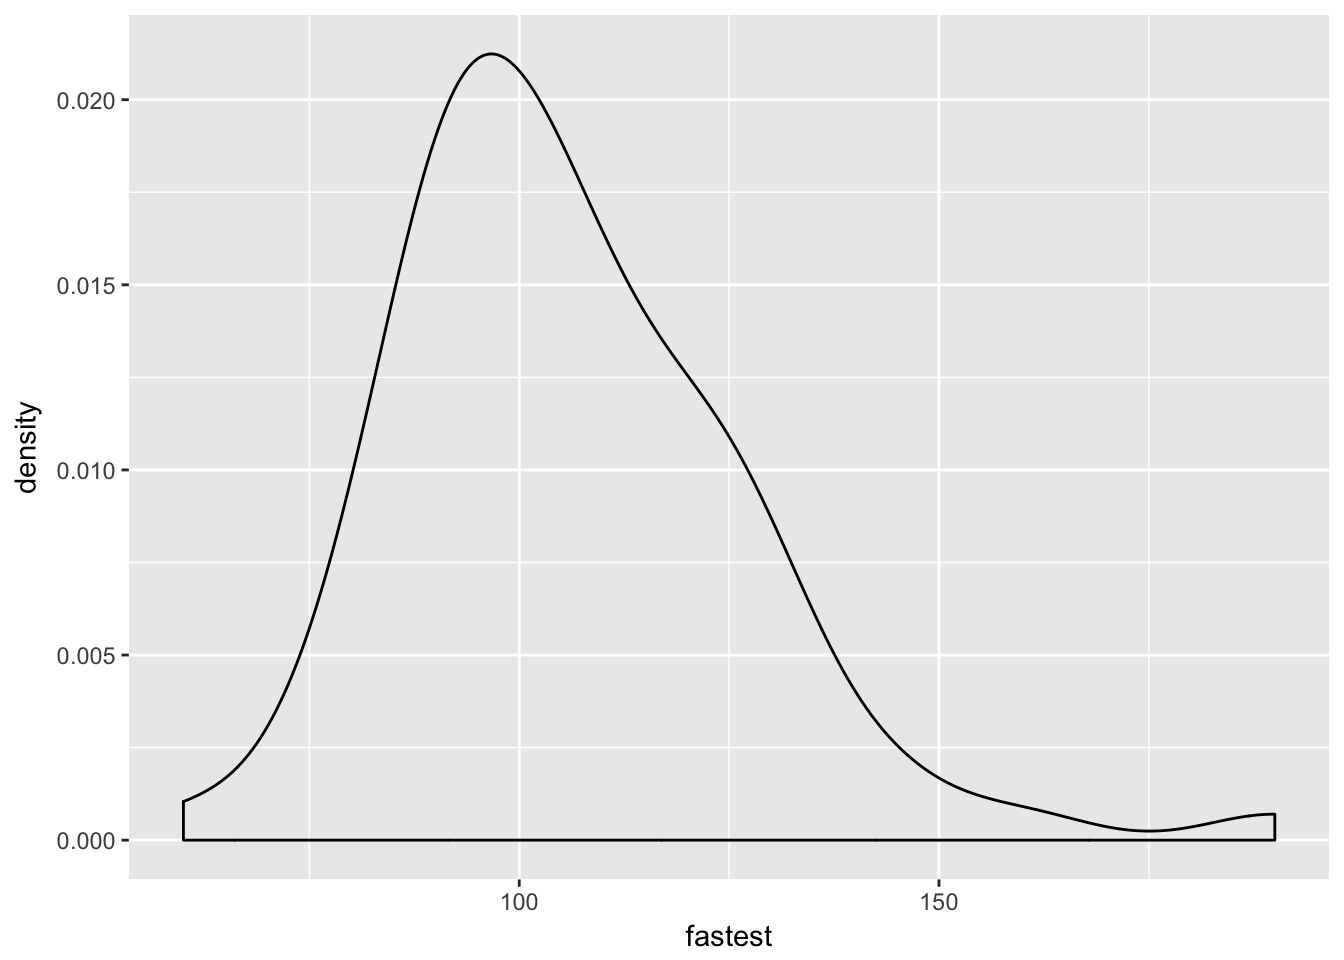
\includegraphics[width=0.6\linewidth]{r-notes_files/figure-latex/fastestdensity-1} 

}

\caption{Basic density plot of the fastest speed every driven.}\label{fig:fastestdensity}
\end{figure}

Recall that the density curve is high where the speeds are crowded
together and lower where they are spread out. Since there are only 71
students in the data set, it's not a bad idea to add a ``rug'' of the
individual speeds to the x-axis. The \texttt{geom\_rug()} function calls
for the rug as another ``shape'' that is added on to the plot:

\begin{Shaded}
\begin{Highlighting}[]
\NormalTok{p <-}\StringTok{ }\NormalTok{p +}\StringTok{ }\KeywordTok{geom_rug}\NormalTok{()}
\end{Highlighting}
\end{Shaded}

It's always good to label the axes of a plot---providing units if
possible---and to add a brief but descriptive title. This is
accomplished by adding labels to the plot with the \texttt{labs()}
function:

\begin{Shaded}
\begin{Highlighting}[]
\NormalTok{p <-}\StringTok{ }\NormalTok{p +}\StringTok{ }\KeywordTok{labs}\NormalTok{(}\DataTypeTok{x =} \StringTok{"Fastest speed ever driven (mph)"}\NormalTok{,}
             \DataTypeTok{title =} \StringTok{"For most students the fastest speed is around 100 mph."}\NormalTok{)}
\end{Highlighting}
\end{Shaded}

Let's print out \texttt{p} again. The result is Figure
\ref{fig:fastestdensity2}.

\begin{Shaded}
\begin{Highlighting}[]
\NormalTok{p}
\end{Highlighting}
\end{Shaded}

\begin{figure}

{\centering 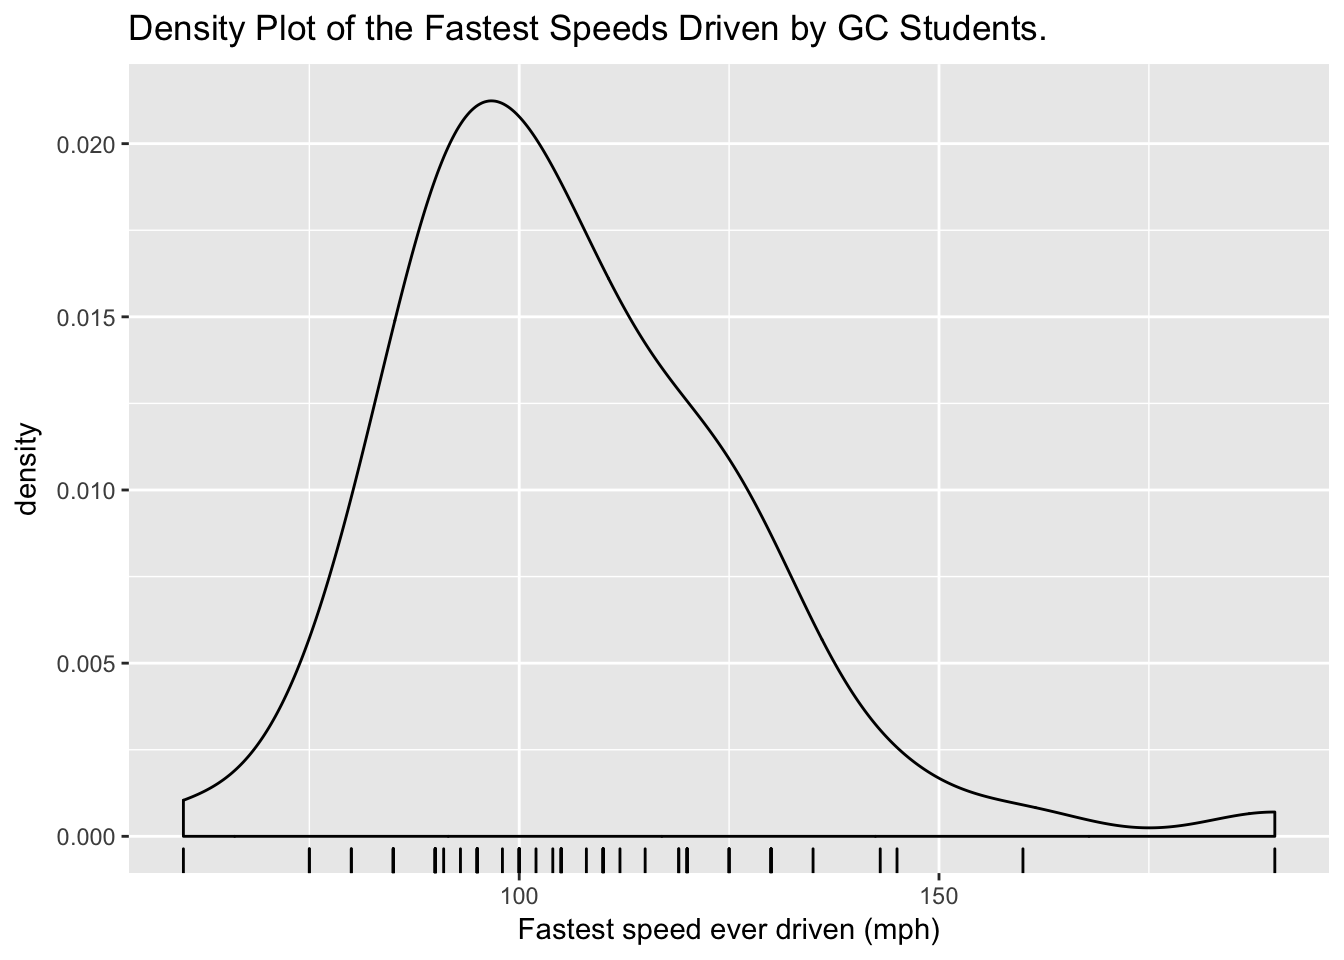
\includegraphics[width=0.6\linewidth]{r-notes_files/figure-latex/fastestdensity2-1} 

}

\caption{Density plot of the fastest speed every driven, with rug and labels.}\label{fig:fastestdensity2}
\end{figure}

Of course the entire plot could be written out in one command:

\begin{Shaded}
\begin{Highlighting}[]
\KeywordTok{ggplot}\NormalTok{(}\DataTypeTok{data =} \NormalTok{m111survey, }\DataTypeTok{mapping =} \KeywordTok{aes}\NormalTok{(}\DataTypeTok{x =} \NormalTok{fastest)) +}
\StringTok{  }\KeywordTok{geom_density}\NormalTok{() +}\StringTok{ }\KeywordTok{geom_rug}\NormalTok{() +}
\StringTok{  }\KeywordTok{labs}\NormalTok{(}\DataTypeTok{x =} \StringTok{"Fastest speed ever driven (mph)"}\NormalTok{,}
             \DataTypeTok{title =} \StringTok{"For most students the fastest speed is around 100 mph"}\NormalTok{)}
\end{Highlighting}
\end{Shaded}

Usually, though, it's a good idea to set up a blank plot with the
\texttt{ggplot()} function and then add to it. In this way one can reuse
the plot-variable, adding different geoms to it, and then stick with the
ones you like best.

For example, you might prefer to make a histogram. Start again with the
blank plot:

\begin{Shaded}
\begin{Highlighting}[]
\NormalTok{p <-}\StringTok{ }\KeywordTok{ggplot}\NormalTok{(}\DataTypeTok{data =} \NormalTok{m111survey, }\DataTypeTok{mapping =} \KeywordTok{aes}\NormalTok{(}\DataTypeTok{x =} \NormalTok{fastest))}
\end{Highlighting}
\end{Shaded}

Now see how a histogram would look (the result is Figure
\ref{fig:fastesthistogram}.)

\begin{Shaded}
\begin{Highlighting}[]
\NormalTok{p +}\StringTok{ }\KeywordTok{geom_histogram}\NormalTok{() +}\StringTok{ }\KeywordTok{geom_rug}\NormalTok{() +}
\StringTok{  }\KeywordTok{labs}\NormalTok{(}\DataTypeTok{x =} \StringTok{"Fastest speed ever driven (mph)"}\NormalTok{,}
             \DataTypeTok{title =} \StringTok{"For most students the fastest speed is around 100 mph"}\NormalTok{)}
\end{Highlighting}
\end{Shaded}

\begin{figure}

{\centering 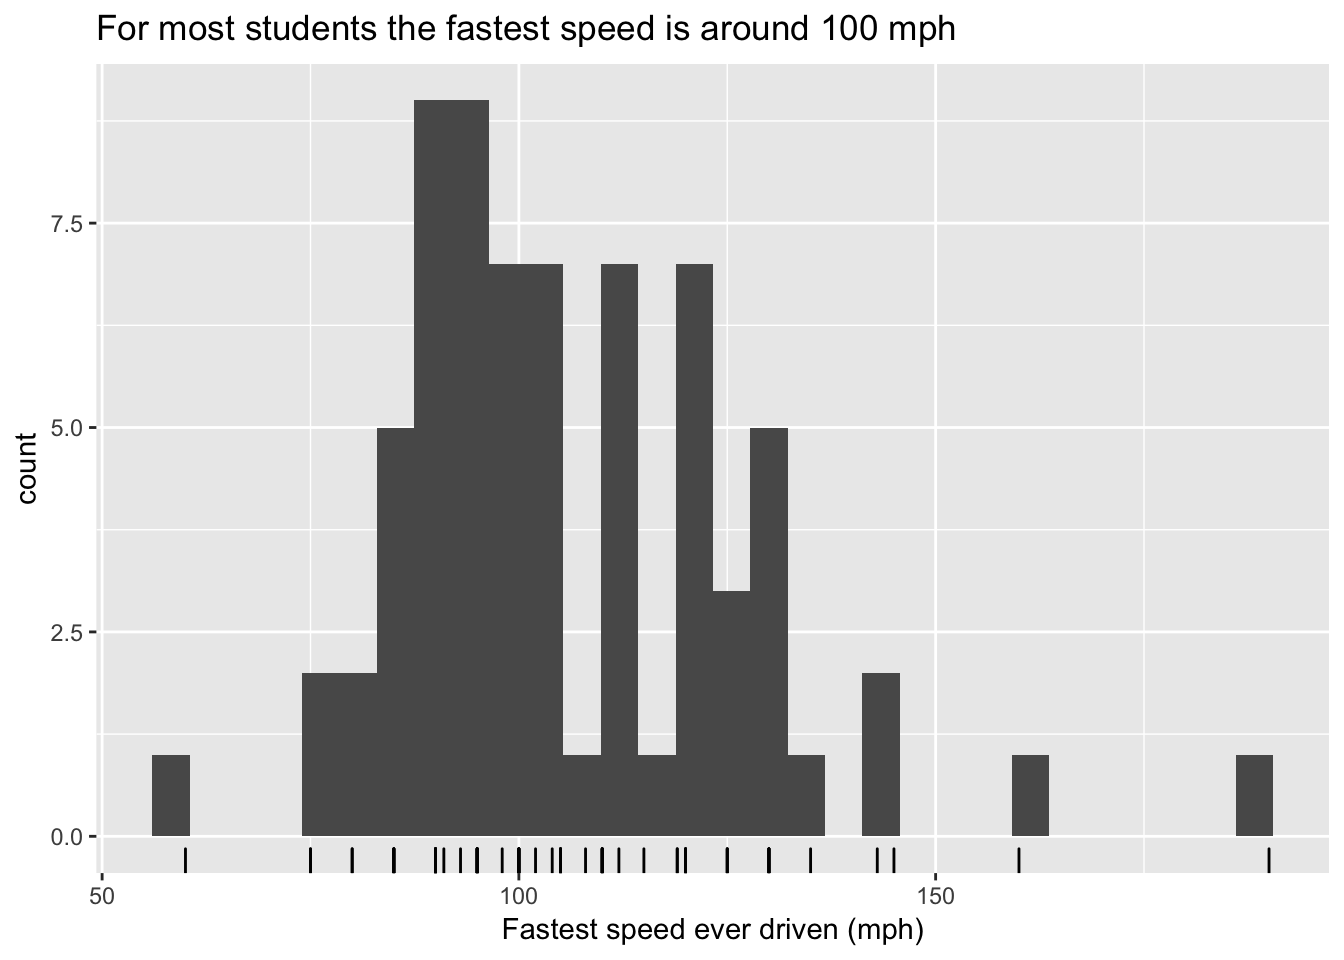
\includegraphics[width=0.6\linewidth]{r-notes_files/figure-latex/fastesthistogram-1} 

}

\caption{Histogram of the fastest speed every driven, with rug and labels.}\label{fig:fastesthistogram}
\end{figure}

If you run code yourself, you see a message to the console:

\begin{verbatim}
##  `stat_bin()` using `bins = 30`. Pick better value with `binwidth`.
\end{verbatim}

\textbf{ggplot2} likes to offer advice: in this case it wants you to
select the width of the histogram-rectangles yourself. This is done with
a \texttt{stat\_bin()} function. Let's make all of our rectangles 10 mph
wide by adding a \texttt{binwidth} argument to
\texttt{geom\_histogram()}. The result is Figure
\ref{fig:fastesthistogram2}.

\begin{Shaded}
\begin{Highlighting}[]
\NormalTok{p +}\StringTok{ }\KeywordTok{geom_histogram}\NormalTok{(}\DataTypeTok{binwidth =} \DecValTok{10}\NormalTok{) +}\StringTok{ }\KeywordTok{geom_rug}\NormalTok{() +}
\StringTok{  }\KeywordTok{labs}\NormalTok{(}\DataTypeTok{x =} \StringTok{"Fastest speed ever driven (mph)"}\NormalTok{,}
             \DataTypeTok{title =} \StringTok{"For most students the fastest speed is around 100 mph"}\NormalTok{)}
\end{Highlighting}
\end{Shaded}

\begin{figure}

{\centering 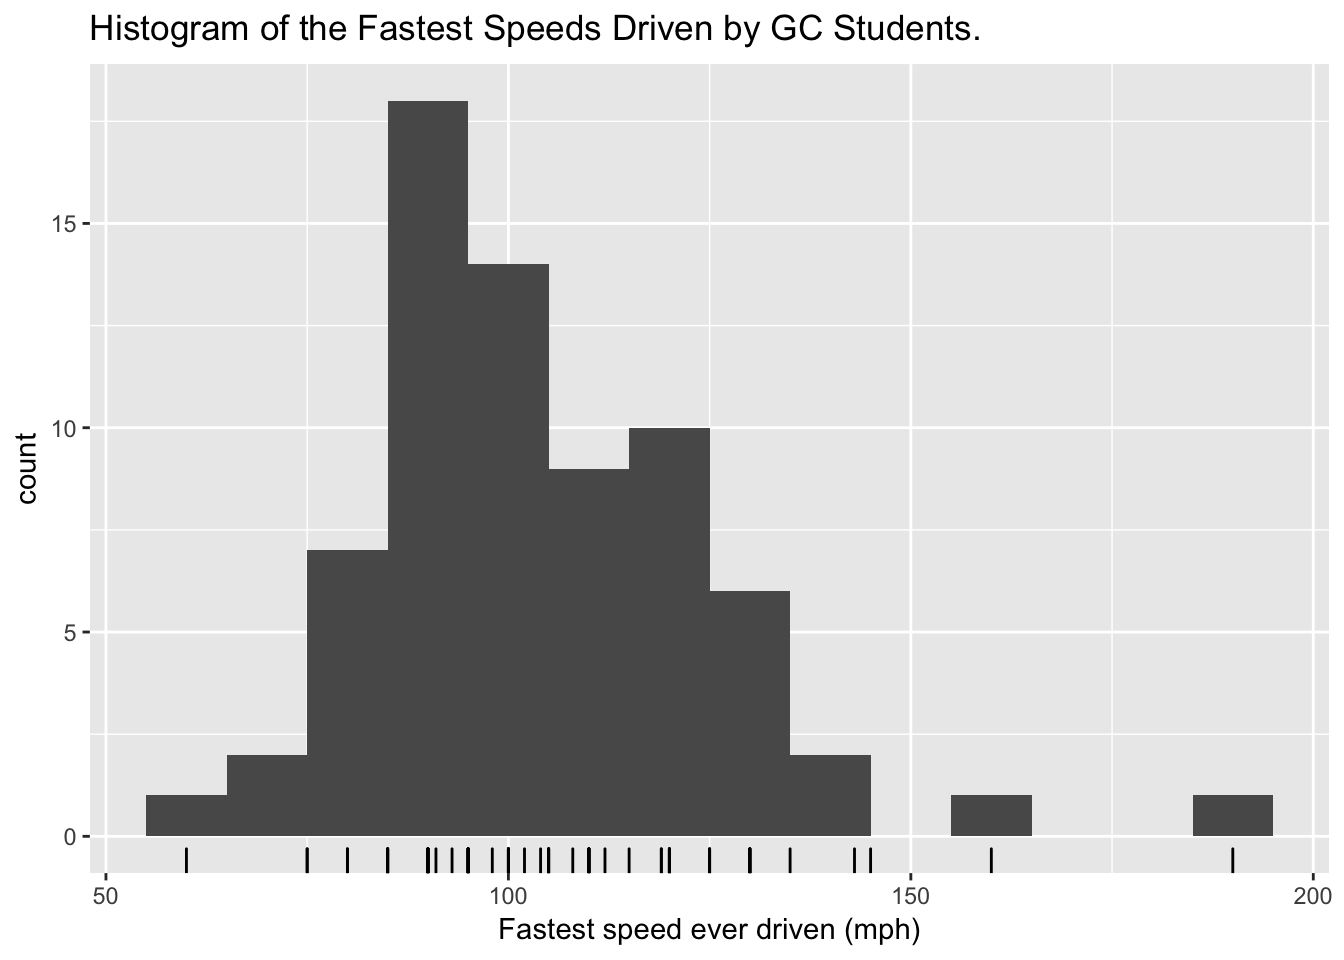
\includegraphics[width=0.6\linewidth]{r-notes_files/figure-latex/fastesthistogram2-1} 

}

\caption{Histogram of the fastest speed every driven, now with binwidth = 10.}\label{fig:fastesthistogram2}
\end{figure}

\subsection{Categorical Variables}\label{categorical-variables}

Beginning with this section we will make only ``rough'' graphs: this is
the way to operate when you are in the process of analyzing data, trying
things out and making discoveries. A proper title, axis-labels and other
refinements can wait until you are polishing your work for publication.

\subsubsection{One Categorical Variable}\label{one-categorical-variable}

In order to study the distribution of a single categorical variable such
as \texttt{seat}, you can make a table:

\begin{Shaded}
\begin{Highlighting}[]
\KeywordTok{with}\NormalTok{(m111survey, }\KeywordTok{table}\NormalTok{(seat))}
\end{Highlighting}
\end{Shaded}

\begin{verbatim}
## seat
##  1_front 2_middle   3_back 
##       27       32       12
\end{verbatim}

You can see the same thing graphically with a bar chart (Figure
\ref{fig:seatbargraph}).

\begin{Shaded}
\begin{Highlighting}[]
\KeywordTok{ggplot}\NormalTok{(m111survey, }\KeywordTok{aes}\NormalTok{(}\DataTypeTok{x =} \NormalTok{seat)) +}\StringTok{ }\KeywordTok{geom_bar}\NormalTok{()}
\end{Highlighting}
\end{Shaded}

\begin{figure}

{\centering 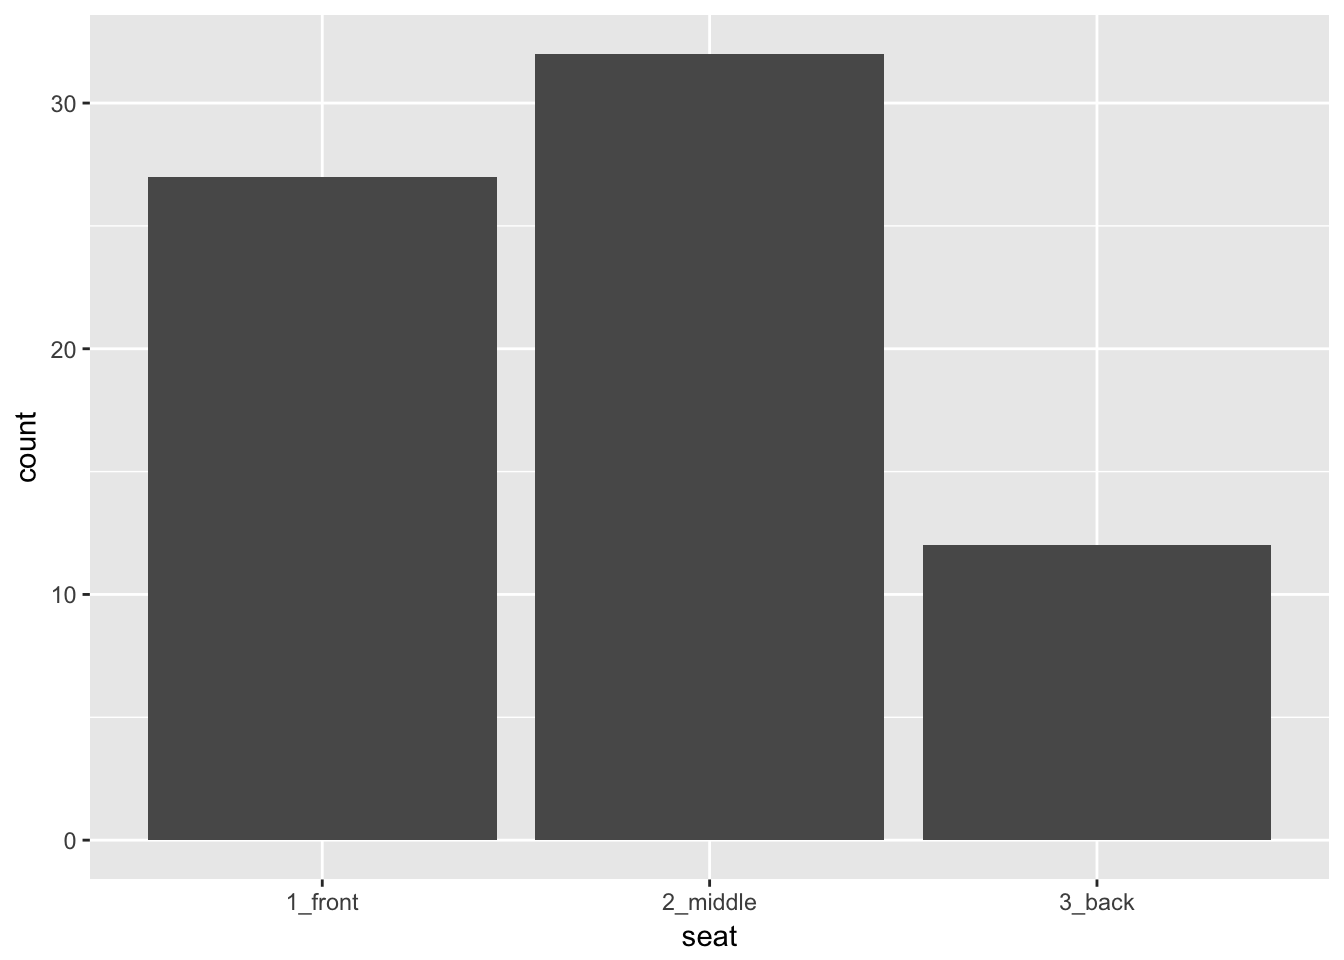
\includegraphics[width=0.6\linewidth]{r-notes_files/figure-latex/seatbargraph-1} 

}

\caption{Bar graph of seating preference.}\label{fig:seatbargraph}
\end{figure}

So far the values of the values of the variable under study have been
shown on the x-axis. Any time you like you can have them appear along
the y-axis, if you add \texttt{coord\_flip()} (see Figure
\ref{fig:seatbargraph2}):

\begin{Shaded}
\begin{Highlighting}[]
\KeywordTok{ggplot}\NormalTok{(m111survey, }\KeywordTok{aes}\NormalTok{(}\DataTypeTok{x =} \NormalTok{seat)) +}\StringTok{ }\KeywordTok{geom_bar}\NormalTok{() +}\StringTok{ }\KeywordTok{coord_flip}\NormalTok{()}
\end{Highlighting}
\end{Shaded}

\begin{figure}

{\centering 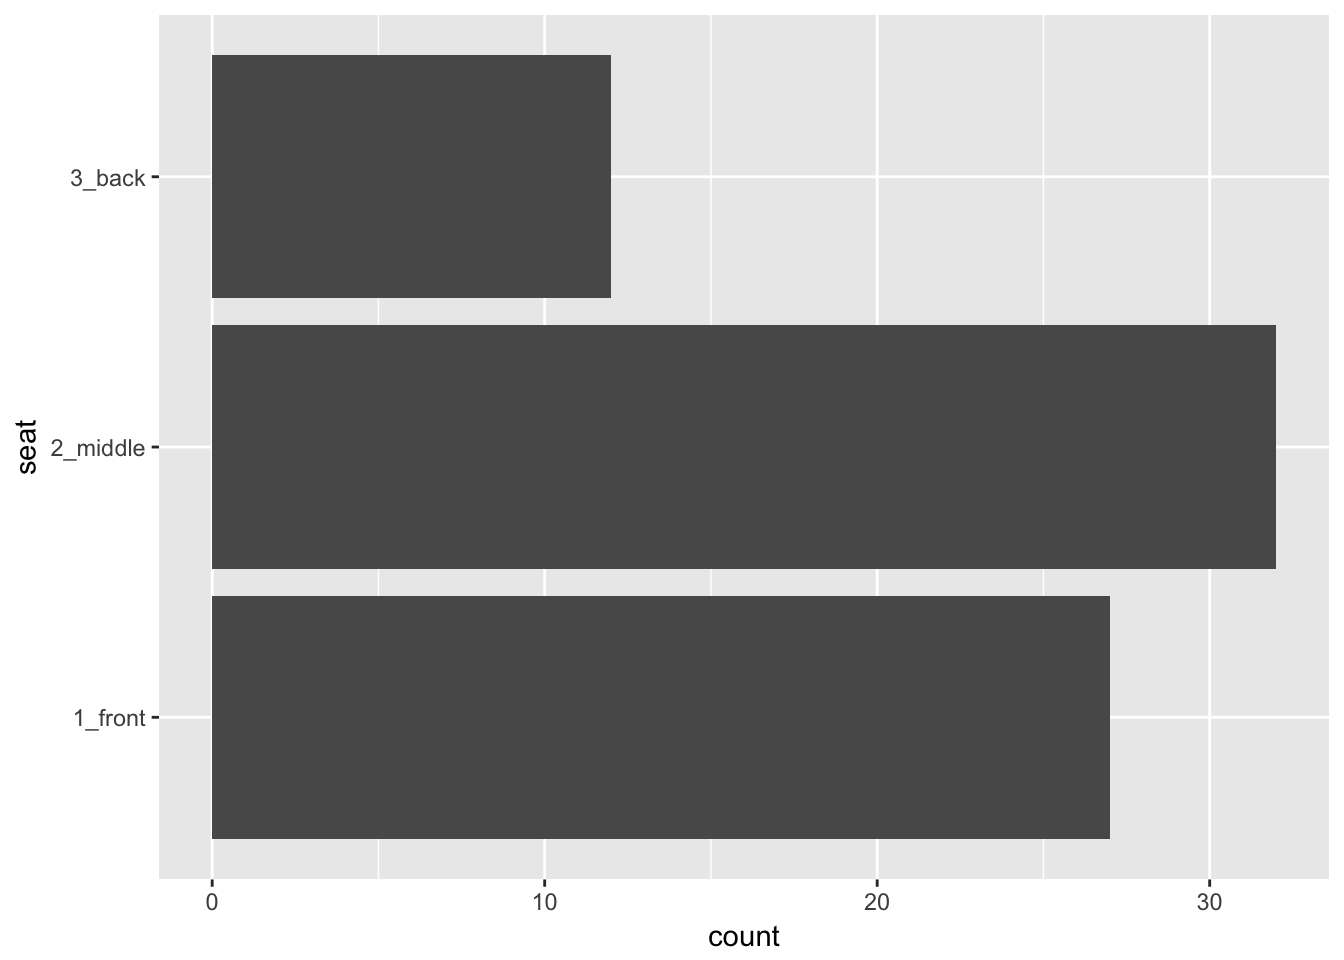
\includegraphics[width=0.6\linewidth]{r-notes_files/figure-latex/seatbargraph2-1} 

}

\caption{Bar graph of seating preference, with coordinates flipped.}\label{fig:seatbargraph2}
\end{figure}

You might get tired of the dark ``fill'' in histograms and bar charts.
The color of the fill is up to you, though. Just set the \texttt{fill}
parameter to the color of your choice. See Figure
\ref{fig:seatbargraph3} for the results of the code below.

\begin{Shaded}
\begin{Highlighting}[]
\KeywordTok{ggplot}\NormalTok{(m111survey, }\KeywordTok{aes}\NormalTok{(}\DataTypeTok{x =} \NormalTok{seat)) +}\StringTok{ }\KeywordTok{geom_bar}\NormalTok{(}\DataTypeTok{fill =} \StringTok{"burlywood"}\NormalTok{)}
\end{Highlighting}
\end{Shaded}

\begin{figure}

{\centering 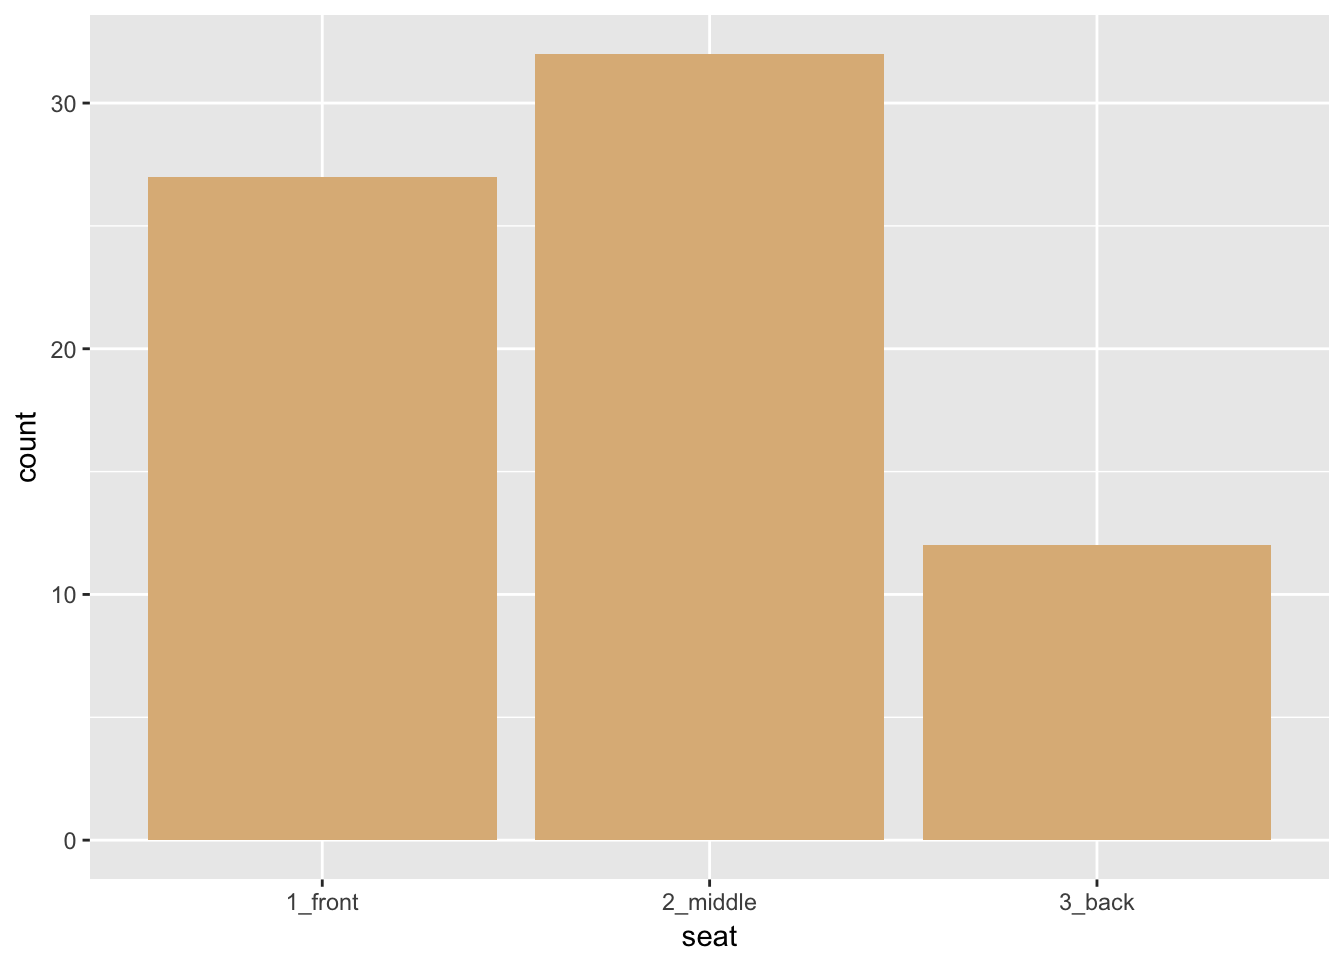
\includegraphics[width=0.6\linewidth]{r-notes_files/figure-latex/seatbargraph3-1} 

}

\caption{Bar graph of seating preference.  The bars have a burlywood fill.}\label{fig:seatbargraph3}
\end{figure}

\subsubsection{Two Categorical
Variables}\label{two-categorical-variables}

Quite often one is interested in comparing two groups of people. For
example, do males and females differ in their seating preferences? One
can investigate this question numerically with a table:

\begin{Shaded}
\begin{Highlighting}[]
\KeywordTok{with}\NormalTok{(m111survey, }\KeywordTok{table}\NormalTok{(sex, seat))}
\end{Highlighting}
\end{Shaded}

\begin{verbatim}
##         seat
## sex      1_front 2_middle 3_back
##   female      19       16      5
##   male         8       16      7
\end{verbatim}

The arguments to \texttt{table()} are the two categorical variables of
interest.

If we want to look into the matter graphically, then we face a
conundrum: there are two categorical variables, but only one x-axis. We
can assign one of the variables to the x-axis in the call to
\texttt{aes()}, but how are we to incorporate the other variable? The
solution lies in a second call to \texttt{aes()}, supplied as an
argument to the desired geom. The code is shown below, and the results
appear as Figure \ref{fig:sexseat1}.

\begin{Shaded}
\begin{Highlighting}[]
\KeywordTok{ggplot}\NormalTok{(m111survey, }\KeywordTok{aes}\NormalTok{(}\DataTypeTok{x =} \NormalTok{sex)) +}\StringTok{ }\KeywordTok{geom_bar}\NormalTok{(}\KeywordTok{aes}\NormalTok{(}\DataTypeTok{fill =} \NormalTok{seat))}
\end{Highlighting}
\end{Shaded}

\begin{figure}

{\centering 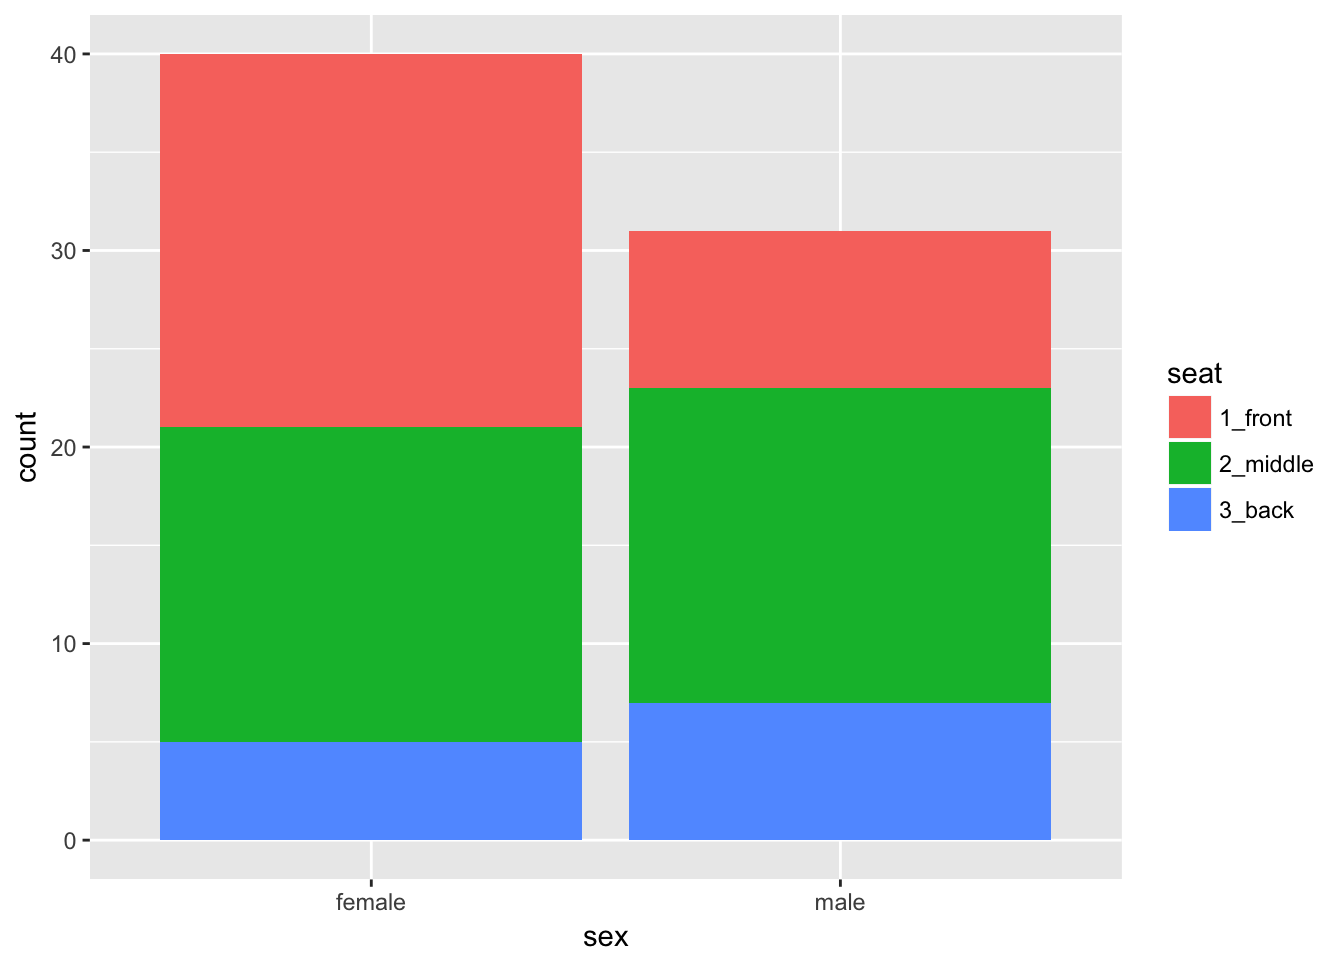
\includegraphics[width=0.6\linewidth]{r-notes_files/figure-latex/sexseat1-1} 

}

\caption{Seating preference, by sex.}\label{fig:sexseat1}
\end{figure}

Within each bar, the proportions of fill-colors indicate the
distribution of seating preference for each gender. It is important to
note the dramatically different roles played by \texttt{fill} in these
two code-snippets:

\begin{itemize}
\tightlist
\item
  \texttt{geom\_bar(fill\ =\ "burlywood")}. In this geom, the fill is
  assigned to be of burlywood color throughout the geom.
\item
  \texttt{geom\_bar(aes(fill\ =\ seat))}. Note that here the fill is
  specified as part of an \emph{aesthetic}, and a categorical
  variable---not a specific color---is assigned to it. This causes
  \textbf{ggplot2} to \emph{map} each level of \texttt{seat} to a
  different color. In this way the variable \texttt{seat} makes its
  presence known in a graph that started out devoted just to the
  variable \texttt{sex}.
\end{itemize}

Some people don't like the colors ``stacked''. In that case, you can set
\texttt{position} to ``dodge'', as in the code below. The results appear
in Figure \ref{fig:sexseat2}.

\begin{Shaded}
\begin{Highlighting}[]
\KeywordTok{ggplot}\NormalTok{(m111survey, }\KeywordTok{aes}\NormalTok{(}\DataTypeTok{x =} \NormalTok{sex)) +}\StringTok{ }
\StringTok{  }\KeywordTok{geom_bar}\NormalTok{(}\KeywordTok{aes}\NormalTok{(}\DataTypeTok{fill =} \NormalTok{seat), }\DataTypeTok{position =}\StringTok{"dodge"}\NormalTok{)}
\end{Highlighting}
\end{Shaded}

\begin{figure}

{\centering 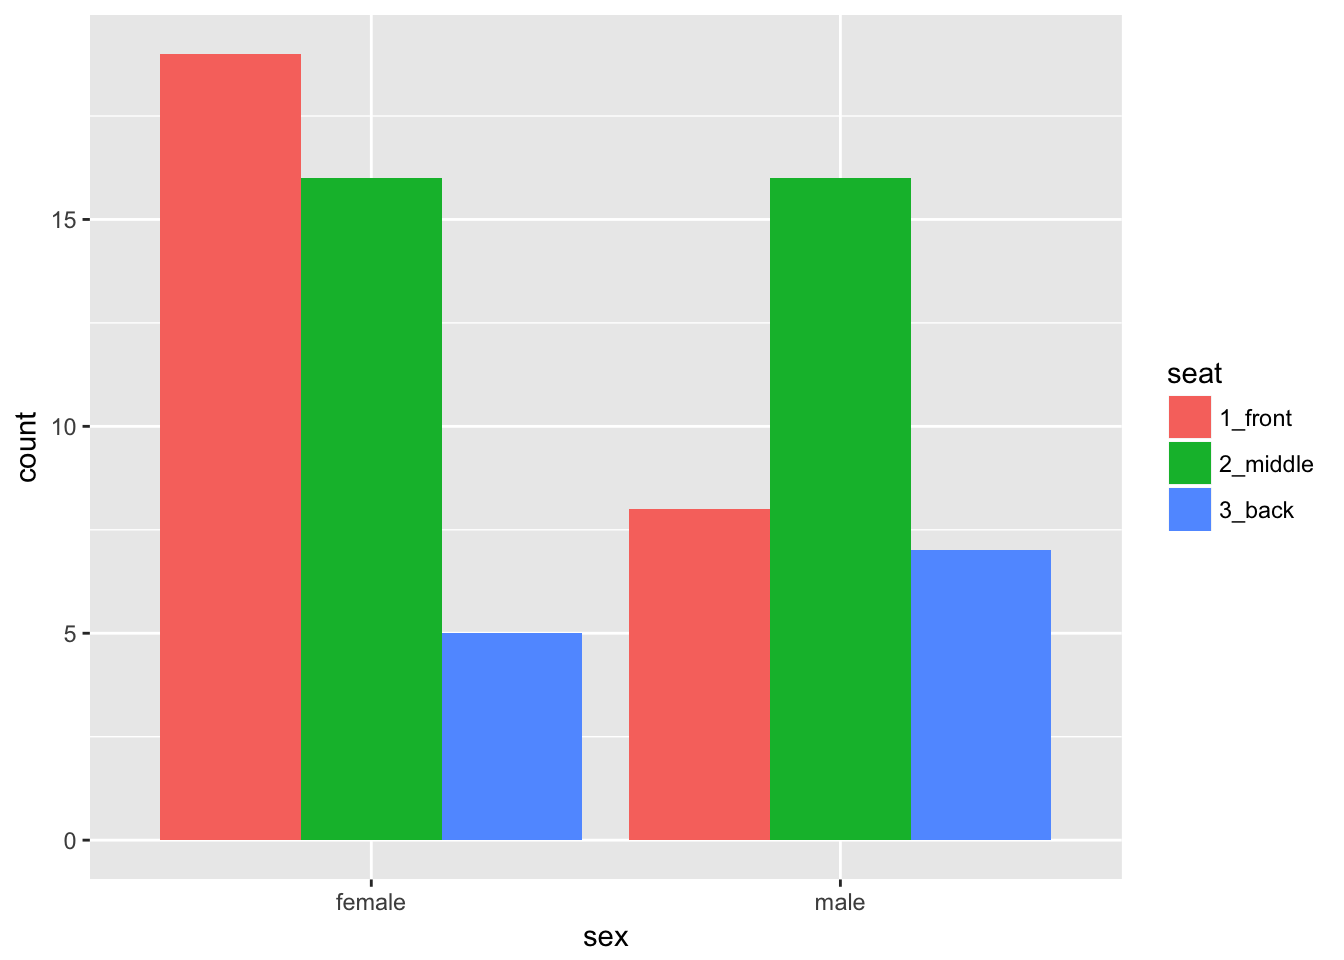
\includegraphics[width=0.6\linewidth]{r-notes_files/figure-latex/sexseat2-1} 

}

\caption{Seating preference, by sex---no stacking of bars..}\label{fig:sexseat2}
\end{figure}

\subsection{One Numerical and One Categorical
Variable}\label{onenum-onecat}

Who tends to drive fastest: people who prefer the Front, the Middle or
the Back? Investigating this question involves comparing the speeds of
three groups of people; more technically we can say that we are asking
about the \emph{relationship} between the numerical variable
\texttt{fastest} and the categorical variable \texttt{seat}.

In this case we can assign one variable to the x-axis and the other to
the y-axis.:

\begin{Shaded}
\begin{Highlighting}[]
\NormalTok{p <-}\StringTok{ }\KeywordTok{ggplot}\NormalTok{(m111survey, }\KeywordTok{aes}\NormalTok{(}\DataTypeTok{x =} \NormalTok{seat, }\DataTypeTok{y =} \NormalTok{fastest))}
\end{Highlighting}
\end{Shaded}

We can now add geoms. We'll make a violin plot---a density curve
mirrored against itself---and an individual-value plot, in which the
individual speeds appear at the appropriate y-axis level, but with their
x-coordinates ``jittered'' randomly so that identical speeds don't
over-plot each other. The graph appears in Figure
\ref{fig:violinfastestseat}. Where a violin is ``thick'' data points are
crowded closely together. Where it is ``thin'', they are more sparse.

\begin{Shaded}
\begin{Highlighting}[]
\NormalTok{p +}\StringTok{ }\KeywordTok{geom_violin}\NormalTok{(}\DataTypeTok{fill =} \StringTok{"burlywood"}\NormalTok{) +}\StringTok{ }\KeywordTok{geom_jitter}\NormalTok{()}
\end{Highlighting}
\end{Shaded}

\begin{figure}

{\centering \includegraphics[width=0.6\linewidth]{r-notes_files/figure-latex/violinfastestseat-1} 

}

\caption{Violin plot of fastest speed by seating preference, with individuals plotted as points.}\label{fig:violinfastestseat}
\end{figure}

Another way to handle the question is to group with a call to
\texttt{aes()} provided to an appropriate geom, as in the code below.
The resulting graph is appears in Figure \ref{fig:fastestseatgrouping}.

\begin{Shaded}
\begin{Highlighting}[]
\KeywordTok{ggplot}\NormalTok{(m111survey, }\KeywordTok{aes}\NormalTok{(}\DataTypeTok{x =} \NormalTok{fastest)) +}\StringTok{ }\KeywordTok{geom_density}\NormalTok{(}\KeywordTok{aes}\NormalTok{(}\DataTypeTok{color =} \NormalTok{seat))}
\end{Highlighting}
\end{Shaded}

\begin{figure}

{\centering \includegraphics[width=0.6\linewidth]{r-notes_files/figure-latex/fastestseatgrouping-1} 

}

\caption{Density plots of fastest speed ever driven, for each seating preference.}\label{fig:fastestseatgrouping}
\end{figure}

\subsection{Two Numerical Variables}\label{two-numerical-variables}

As we have seen in previous chapters, scatter plots are a fine way to
visualize the relationship between two numerical variables. In our call
to \texttt{aes()} we simply assign one of the variables to the x-axis
and the other to the y-axis. A scatter plot showing the relationship
between grade=point average and fastest speed ever driven is shown in
Figure \ref{fig:fastestGPAseatA}.

\begin{Shaded}
\begin{Highlighting}[]
\NormalTok{p <-}\StringTok{ }\KeywordTok{ggplot}\NormalTok{(m111survey, }\KeywordTok{aes}\NormalTok{(}\DataTypeTok{x =} \NormalTok{fastest, }\DataTypeTok{y =} \NormalTok{GPA)) +}\StringTok{ }\KeywordTok{geom_point}\NormalTok{(}\DataTypeTok{na.rm =} \NormalTok{T)}
\NormalTok{p}
\end{Highlighting}
\end{Shaded}

\begin{figure}

{\centering \includegraphics[width=0.6\linewidth]{r-notes_files/figure-latex/fastestGPAseatA-1} 

}

\caption{Scatter plot of GPA vs. fastest speed ever driven. Students who drive faster tend to have lower GPAs.}\label{fig:fastestGPAseatA}
\end{figure}

\subsection{Grouping by a Categorical
Variable}\label{grouping-by-a-categorical-variable}

It is possible to incorporate a third variable into our plot. As with
the bar geoms---or any other geom---this is accomplished by mapping
through an aesthetic parameter. The code below uses the color of the
points to represent the levels of the variable \texttt{seat}. The
scatter plot itself is shown in Figure \ref{fig:fastestGPAseat}.

\begin{Shaded}
\begin{Highlighting}[]
\NormalTok{p +}\StringTok{ }\KeywordTok{geom_point}\NormalTok{(}\KeywordTok{aes}\NormalTok{(}\DataTypeTok{color =} \NormalTok{seat), }\DataTypeTok{na.rm =} \NormalTok{T)}
\end{Highlighting}
\end{Shaded}

\begin{figure}

{\centering \includegraphics[width=0.6\linewidth]{r-notes_files/figure-latex/fastestGPAseat-1} 

}

\caption{Scatter plot of GPA vs. fastest speed ever driven, with individuals grouped by seating preference.}\label{fig:fastestGPAseat}
\end{figure}

Evidently the people who prefer the back tend to drive pretty fast and
to have lower grade-point averages!

\subsection{Application: U.S. Births}\label{application-u.s.-births}

In Section \ref{idea-data}, we made a plot of the number of births in
the United States for each day of that year (see Figure
\ref{fig:birthsplotframes}). We noticed that there appear to be two
clouds of points. What accounts for this phenomenon? By now we have the
R-programming chops to take on this question.

\begin{figure}

{\centering \includegraphics[width=0.6\linewidth]{r-notes_files/figure-latex/birthsplotframes-1} 

}

\caption{Some of the days have significantly fewer births.  What's going on?}\label{fig:birthsplotframes}
\end{figure}

To begin with, look at all of the variables available in the data frame
\texttt{Births78}:

\begin{Shaded}
\begin{Highlighting}[]
\KeywordTok{str}\NormalTok{(Births78)}
\end{Highlighting}
\end{Shaded}

\begin{verbatim}
## 'data.frame':    365 obs. of  5 variables:
##  $ date     : POSIXct, format: "1978-01-01" "1978-01-02" ...
##  $ births   : int  7701 7527 8825 8859 9043 9208 8084 7611 9172 9089 ...
##  $ dayofyear: int  1 2 3 4 5 6 7 8 9 10 ...
##  $ wday     : Ord.factor w/ 7 levels "Sun"<"Mon"<"Tues"<..: 1 2 3 4 5 6 7 1 2 3 ...
##  $ weekend  : chr  "weekend" "weekday" "weekday" "weekday" ...
\end{verbatim}

We see that the variable \texttt{wday} gives the name of the day of the
week, for each of the days in the year. On a hunch, we make violin plots
of the births for each of the days of the week. The code appears below,
and the resulting plot is shown in Figure \ref{fig:violinbirthswday}

\begin{Shaded}
\begin{Highlighting}[]
\KeywordTok{ggplot}\NormalTok{(Births78, }\KeywordTok{aes}\NormalTok{(}\DataTypeTok{x =} \NormalTok{wday, }\DataTypeTok{y =} \NormalTok{births)) +}\StringTok{ }\KeywordTok{geom_violin}\NormalTok{(}\DataTypeTok{fill =} \StringTok{"burlywood"}\NormalTok{) +}
\StringTok{  }\KeywordTok{geom_jitter}\NormalTok{()}
\end{Highlighting}
\end{Shaded}

\begin{figure}

{\centering \includegraphics[width=0.6\linewidth]{r-notes_files/figure-latex/violinbirthswday-1} 

}

\caption{Violin plot of births, by day of the week.}\label{fig:violinbirthswday}
\end{figure}

Aha! There are considerably fewer births on the weekend-days---Saturday
and Sunday. Perhaps the \emph{entire} lower cloud of points is composed
of weekends. Let's check this by re-coding the days according to whether
or not they are during the week or at the weekend:

\begin{Shaded}
\begin{Highlighting}[]
\NormalTok{weekend <-}\StringTok{ }\KeywordTok{with}\NormalTok{(Births78, }\KeywordTok{ifelse}\NormalTok{(wday %in%}\StringTok{ }\KeywordTok{c}\NormalTok{(}\StringTok{"Sat"}\NormalTok{,}\StringTok{"Sun"}\NormalTok{),}
                                 \StringTok{"weekend"}\NormalTok{, }\StringTok{"weekday"}\NormalTok{))}
\NormalTok{Births78$weekend <-}\StringTok{ }\NormalTok{weekend}
\end{Highlighting}
\end{Shaded}

Note that we have added the new variable to the data frame, so that it
will be easy in \textbf{ggplot2} to use that variable for grouping, as
in the code below. The results appear in Figure
\ref{fig:birthsplotframesweekend}.

\begin{Shaded}
\begin{Highlighting}[]
\KeywordTok{ggplot}\NormalTok{(Births78, }\KeywordTok{aes}\NormalTok{(}\DataTypeTok{x =} \NormalTok{date, }\DataTypeTok{y =} \NormalTok{births)) +}\StringTok{ }\KeywordTok{geom_point}\NormalTok{(}\KeywordTok{aes}\NormalTok{(}\DataTypeTok{color =} \NormalTok{weekend)) +}
\StringTok{  }\KeywordTok{labs}\NormalTok{(}\DataTypeTok{x =} \StringTok{"Day of the Year"}\NormalTok{, }\DataTypeTok{y =} \StringTok{"Number of U.S. Births"}\NormalTok{,}
       \DataTypeTok{title =} \StringTok{"Daily U.S. Birth-Numbers in 1978"}\NormalTok{)}
\end{Highlighting}
\end{Shaded}

\begin{figure}

{\centering \includegraphics[width=0.6\linewidth]{r-notes_files/figure-latex/birthsplotframesweekend-1} 

}

\caption{The days with fewer births are almost always weekend-days.}\label{fig:birthsplotframesweekend}
\end{figure}

Well, a \emph{few} of the points in the lower cloud are weekdays. Is
there anything special about them? To find out, we subset the data frame
to examine only those points:

\begin{Shaded}
\begin{Highlighting}[]
\NormalTok{df <-}\StringTok{ }\KeywordTok{subset}\NormalTok{(Births78, weekend !=}\StringTok{ "weekend"} \NormalTok{&}\StringTok{ }\NormalTok{births <=}\StringTok{ }\DecValTok{8500}\NormalTok{)}
\NormalTok{df}
\end{Highlighting}
\end{Shaded}

\begin{verbatim}
##           date births dayofyear  wday weekend
## 2   1978-01-02   7527         2   Mon weekday
## 149 1978-05-29   7780       149   Mon weekday
## 185 1978-07-04   8433       185  Tues weekday
## 247 1978-09-04   8481       247   Mon weekday
## 327 1978-11-23   7915       327 Thurs weekday
## 359 1978-12-25   7846       359   Mon weekday
\end{verbatim}

If you consult a calendar for the year 1978, you will find that every
one of the above days was a major holiday. Apparently doctors prefer not
to deliver babies on weekend and holidays. Scheduled births---induced
births or births by non-emergency Cesarean section---are not usually set
for weekends or holidays. Perhaps this accounts for the two clouds we
saw in the original scatter plot.

\subsection{Learn More}\label{learn-more}

From time to time we will return to \textbf{gplot2} and deepen our study
of this remarkable graphing system. If you are impatient to learn more
right way, you can explore the package's
\href{http://docs.ggplot2.org/current/index.html}{documentation site}.
The site teaches the system by way of numerous examples that you can
copy and modify.

\newpage

\section*{Glossary}\label{glossary-5}
\addcontentsline{toc}{section}{Glossary}

\begin{description}
\item[Matrix \index{matrix}]
An atomic vector that has two additional attributes: a number of rows
and a number of columns.
\item[Data Frame \index{data frame}]
A two-dimensional data structure in R in which the columns are atomic
vectors that can be of different types.
\item[Case (also called an Individual) \index{case}]
An individual unit under study. In a data frame in R, the rows
correspond to cases.
\item[Variable (in Data Analysis)]
In data analysis, a \emph{variable} is a measurement made on the
individuals in a study.
\item[Categorical Variable (in Data Analysis)]
In data analysis, a \emph{categorical variable} is a variable whose
values cannot be expressed meaningfully by numbers.
\end{description}

\newpage

\hypertarget{frames-exercises}{\section*{Exercises}\label{frames-exercises}}
\addcontentsline{toc}{section}{Exercises}

\begin{center}\includegraphics[width=0.5\linewidth]{images/thinking} \end{center}

\begin{enumerate}
\def\labelenumi{\arabic{enumi}.}
\item
  R has a function called \texttt{t()} that computes the
  \emph{transpose} of a given matrix. This means that it switches around
  the rows and columns of the matrix, like this:

\begin{Shaded}
\begin{Highlighting}[]
\NormalTok{myMatrix <-}\StringTok{ }\KeywordTok{matrix}\NormalTok{(}\DecValTok{1}\NormalTok{:}\DecValTok{24}\NormalTok{, }\DataTypeTok{nrow =} \DecValTok{6}\NormalTok{)}
\NormalTok{myMatrix}
\end{Highlighting}
\end{Shaded}

\begin{verbatim}
##      [,1] [,2] [,3] [,4]
## [1,]    1    7   13   19
## [2,]    2    8   14   20
## [3,]    3    9   15   21
## [4,]    4   10   16   22
## [5,]    5   11   17   23
## [6,]    6   12   18   24
\end{verbatim}

\begin{Shaded}
\begin{Highlighting}[]
\KeywordTok{t}\NormalTok{(myMatrix)}
\end{Highlighting}
\end{Shaded}

\begin{verbatim}
##      [,1] [,2] [,3] [,4] [,5] [,6]
## [1,]    1    2    3    4    5    6
## [2,]    7    8    9   10   11   12
## [3,]   13   14   15   16   17   18
## [4,]   19   20   21   22   23   24
\end{verbatim}

  Write your own function called \texttt{transpose()} that will perform
  the same task on any given matrix. The function should take a single
  parameter called \texttt{mat}, the matrix to be transposed. \textbf{Of
  course you may NOT use \texttt{t()} in the code for your function!}
\item
  R has functions called \texttt{rowSums()} and \texttt{colSums()} that
  will respectively sum the rows and the columns of a matrix. Here is an
  example:

\begin{Shaded}
\begin{Highlighting}[]
\NormalTok{myMatrix <-}\StringTok{ }\KeywordTok{matrix}\NormalTok{(}\DecValTok{1}\NormalTok{:}\DecValTok{24}\NormalTok{, }\DataTypeTok{nrow =} \DecValTok{6}\NormalTok{)}
\KeywordTok{rowSums}\NormalTok{(myMatrix)}
\end{Highlighting}
\end{Shaded}

\begin{verbatim}
## [1] 40 44 48 52 56 60
\end{verbatim}

  Your task is to write your own function called \texttt{dimSum()} that
  will sum either the rows or the columns of a given matrix. The
  function should have two parameters:

  \begin{itemize}
  \tightlist
  \item
    \texttt{mat}: the matrix to be summed.
  \item
    \texttt{dim}: the dimension to sum along, either rows or columns.
    The default value should be \texttt{c("rows",\ "columns")}, and you
    should use \protect\hyperlink{argument-matching}{argument-matching}
    so that the user doesn't have to spell out all of the possible
    arguments.
  \end{itemize}

  \textbf{You may NOT use \texttt{rowSums()} or \texttt{colSums()} in
  the code for your function.} A typical example of use should look like
  this:

\begin{Shaded}
\begin{Highlighting}[]
\NormalTok{myMatrix <-}\StringTok{ }\KeywordTok{matrix}\NormalTok{(}\DecValTok{1}\NormalTok{:}\DecValTok{24}\NormalTok{, }\DataTypeTok{nrow =} \DecValTok{6}\NormalTok{)}
\KeywordTok{dimSum}\NormalTok{(myMatrix, }\StringTok{"c"}\NormalTok{)}
\end{Highlighting}
\end{Shaded}

\begin{verbatim}
## [1]  21  57  93 129
\end{verbatim}
\item
  The next few exercises pertain to the data frame \texttt{CPS85} from
  the package \textbf{mosaicData}. Learn about it with
  \texttt{help(CPS85)}. We will use the \textbf{ggplot2} graphing
  package to explore whether men were being paid more than women in
  1985.

  Make a density plot of the wages of the people in the study. As with
  all plot you make, it should have well-labelled axes (with units if
  possible). For a density plot you should label the horizontal axis,
  but you can let \textbf{ggplo2} provide the label for the ``density''
  axis. As always, provide a descriptive title. Also provide a ``rug''
  of individual values along the horizontal axis.
\item
  Look at the plot you made in the previous exercise: you will notice
  that one person made a wage that was much higher than all the rest. In
  data analysis, when a value is much higher or lower than the rest of
  the values we call it an \emph{outlier}.

  Write the code needed to find the age, sex and sector of employment of
  the person who made this extraoridinarily high wage. Report the age,
  sex and sector of this person.

  Create a new data frame called \texttt{cpsSmall} that is the same as
  \texttt{CPC85} execept that it excludes the row corresponding to the
  outlier-individual.
\item
  In order to explore the relationship between wage and sex in the CPS
  study, make violin plots for the wages of men and women. (In this
  exercise and in subsequent exercises, use the \texttt{cpsSmall} data
  frame so as to exclude the outlier. You can produce the plot by
  modifying the code for the ``fastest speed vs.~seating'' plot in
  Section \ref{onenum-onecat}.) Based on the plot, who tends to earn
  higher wages: men or women?
\item
  Someone might argue that men don't earn higher wages because of
  sex-discrimination in the workplace, but rather because of some other
  factor. For example, it could be that in 1985 women chose to work in
  low-wage sectors of the economy, whereas men tended to work in
  higher-wage sectors. Of course for this explanation to be viable, some
  sectors of the economy have to pay more on average than other sectors
  do. In order to verify whether this is the case, make a violin plot of
  wage vs.~sector of employment. Use the plot to name a couple of
  high-wage sectors and a couple of low-wage sectors.
\item
  From the previous exercise you now know that some sectors of the
  economy pay more than other sectors. Hence in order to investigate
  properly whether there was wage-discrimination in the wrokforce based
  on sex, we would have to compare the wages of men and women who work
  in the \emph{same} sector. To this end it would be nice to have eight
  separate violin plots, one for each sector. Each plot would compare
  the wages of men and women in that sector. Go to the online
  \textbf{ggplot2} documentation and look up \texttt{facet\_wrap()}. Use
  it to construct a graph that displays all eight plots at once.

  Examine your graph.

  \begin{itemize}
  \tightlist
  \item
    Are there any sectors in which it seems that women typically make
    more than men. If so, what sectors are they?
  \item
    On the other hand, are there any sectors where men typically make
    more than women? If so, what sectors are they?
  \item
    Based on your analysis, does it seem plausible that women made less
    than men simply because they chose lower-paying sectors of
    employment?
  \end{itemize}
\item
  The next few exercises pertain to the data frame \texttt{imagpop} in
  the \textbf{tigerstats} package. Learn about it with
  \texttt{help(imagpop)}.

  One of the variables in \texttt{imagpop} is \texttt{kkardashtemp}, the
  rating given by each person to the celebrity Kim Kardashian. Make a
  density plot of the ratings. Compute the mean Kim Kardashian raintg
  for all the people in \texttt{imagpop}. Finally, compute the
  percentage of people in the population who gave a rating more than 40
  but less than 60.
\item
  Write a program that repeats the following procedure 100 times:

  \begin{itemize}
  \tightlist
  \item
    Randomly select 10 people from the population.
  \item
    Compute the mean \texttt{kkardashtemp} rating for these 10 people.
  \end{itemize}

  The means should be stored in a numerical vector. Make a density plot
  (with rug) of the means, and also compute the percentage of the means
  that are between 40 and 60. As always, the plot should have sensible
  labels and a descriptive title.
\item
  Use matrices to generalize the simulation in the Appeals Court Paradox
  (see Section \ref{appeals-court-paradox}). Your goal is to write a
  simulation function called \texttt{appealsSimPlus()} that comes with
  all the options provided in the text, but with additional parameters
  so that the user can choose:

  \begin{itemize}
  \tightlist
  \item
    the number of judges on the court;
  \item
    the probability for each judge to make a correct decision;
  \item
    the voting pattern (how many votes each judge gets).
  \end{itemize}

  A typical call to the functions should look like this:

\begin{Shaded}
\begin{Highlighting}[]
\KeywordTok{appealsSimPlus}\NormalTok{(}\DataTypeTok{reps =} \DecValTok{10000}\NormalTok{, }\DataTypeTok{seed =} \DecValTok{5252}\NormalTok{, }
               \DataTypeTok{probs =} \KeywordTok{c}\NormalTok{(}\FloatTok{0.95}\NormalTok{, }\FloatTok{0.90}\NormalTok{, }\FloatTok{0.90}\NormalTok{, }\FloatTok{0.90}\NormalTok{, }\FloatTok{0.80}\NormalTok{),}
               \DataTypeTok{votes =} \KeywordTok{c}\NormalTok{(}\DecValTok{2}\NormalTok{, }\DecValTok{1}\NormalTok{, }\DecValTok{1}\NormalTok{, }\DecValTok{1}\NormalTok{, }\DecValTok{0}\NormalTok{))}
\end{Highlighting}
\end{Shaded}

  In the above call the court consists of five judges. The best one
  decides cases correctly 95\% of the time, three are right 90\% of the
  time and one is right 80\%of the time. The voting arrangement is that
  the best judge gets two votes, the next three get one vote each, and
  the worst gets no vote. Any voting scheme---even a scheme involving
  fractional votes---should be allowed so long as the votes add up to
  the number of judges.

  \textbf{Here is a hint.} When you write the function it may be helpful
  to use the fact that \texttt{rbinom()} can take a \texttt{prob}
  parameter that is a vector of any length. Here's an example:

\begin{Shaded}
\begin{Highlighting}[]
\NormalTok{results <-}\StringTok{ }\KeywordTok{rbinom}\NormalTok{(}\DecValTok{6}\NormalTok{, }\DataTypeTok{size =} \DecValTok{100}\NormalTok{, }\DataTypeTok{prob =} \KeywordTok{c}\NormalTok{(}\FloatTok{0.10}\NormalTok{, }\FloatTok{0.50}\NormalTok{, }\FloatTok{0.90}\NormalTok{))}
\NormalTok{results}
\end{Highlighting}
\end{Shaded}

\begin{verbatim}
## [1] 20 49 94 15 50 88
\end{verbatim}

  The first and fourth entries simulate a person tossing a fair coin 100
  times when she has only a 10\% chance of heads. The second and fifth
  entries simulate the same, when the chance of heads is 50\%. The third
  and sixth simulate coin-tossing when there is a 90\% chance of heads.

  If you would like to arrange the results more nicely---say in a matrix
  where each column gives the results for a different person---you can
  do so:

\begin{Shaded}
\begin{Highlighting}[]
\NormalTok{resultsMat <-}\StringTok{ }\KeywordTok{matrix}\NormalTok{(results, }\DataTypeTok{ncol =} \DecValTok{3}\NormalTok{, }\DataTypeTok{byrow =} \NormalTok{T)}
\NormalTok{resultsMat}
\end{Highlighting}
\end{Shaded}

\begin{verbatim}
##      [,1] [,2] [,3]
## [1,]   20   49   94
## [2,]   15   50   88
\end{verbatim}

  Of course judges don't flip a coin 100 times, they decide one case at
  a time. Suppose you have five judges with probabilities as follows:

\begin{Shaded}
\begin{Highlighting}[]
\NormalTok{probCorrect <-}\StringTok{ }\KeywordTok{c}\NormalTok{(}\FloatTok{0.95}\NormalTok{, }\FloatTok{0.90}\NormalTok{, }\FloatTok{0.90}\NormalTok{, }\FloatTok{0.90}\NormalTok{, }\FloatTok{0.80}\NormalTok{)}
\end{Highlighting}
\end{Shaded}

  If you would like to simulate the judges deciding, say, 6 cases, try
  this:

\begin{Shaded}
\begin{Highlighting}[]
\NormalTok{results <-}\StringTok{ }\KeywordTok{rbinom}\NormalTok{(}\DecValTok{5}\NormalTok{*}\DecValTok{6}\NormalTok{, }\DataTypeTok{size =} \DecValTok{1}\NormalTok{, }\DataTypeTok{prob=} \KeywordTok{rep}\NormalTok{(probCorrect, }\DecValTok{6}\NormalTok{))}
\NormalTok{resultsMat <-}\StringTok{ }\KeywordTok{matrix}\NormalTok{(results, }\DataTypeTok{nrow =} \DecValTok{6}\NormalTok{, }\DataTypeTok{byrow =} \NormalTok{T)}
\NormalTok{resultsMat}
\end{Highlighting}
\end{Shaded}

\begin{verbatim}
##      [,1] [,2] [,3] [,4] [,5]
## [1,]    1    1    1    0    1
## [2,]    0    1    1    1    1
## [3,]    1    1    1    1    1
## [4,]    1    1    1    1    1
## [5,]    1    1    1    1    1
## [6,]    1    1    1    1    0
\end{verbatim}

  When it comes to applying the voting pattern to compute the decision
  in each case, consider matrix multiplication. For example, suppose
  that the pattern is:

\begin{Shaded}
\begin{Highlighting}[]
\NormalTok{votes <-}\StringTok{ }\KeywordTok{c}\NormalTok{(}\DecValTok{2}\NormalTok{, }\DecValTok{1}\NormalTok{, }\DecValTok{1}\NormalTok{, }\DecValTok{1}\NormalTok{, }\DecValTok{0}\NormalTok{)}
\end{Highlighting}
\end{Shaded}

  Then make \texttt{votes} a one-column matrix and perform matrix
  multiplication:

\begin{Shaded}
\begin{Highlighting}[]
\NormalTok{correctVotes <-}\StringTok{ }\NormalTok{resultsMat %*%}\StringTok{ }\KeywordTok{matrix}\NormalTok{(votes, }\DataTypeTok{nrow =} \DecValTok{5}\NormalTok{)}
\NormalTok{correctVotes}
\end{Highlighting}
\end{Shaded}

\begin{verbatim}
##      [,1]
## [1,]    4
## [2,]    3
## [3,]    5
## [4,]    5
## [5,]    5
## [6,]    5
\end{verbatim}

  Think about how to encapsulate all of this into a nice, general
  simulation function.
\end{enumerate}

\chapter{Lists}\label{lists}

\begin{center}\includegraphics[width=0.6\linewidth]{images/santa-list} \end{center}

In this Chapter we will study \emph{lists}, another important data
structure in R.

\newpage

\section{Introduction to Lists}\label{introduction-to-lists}

So far the vectors that we have met have all been \emph{atomic}, meaning
that they can hold only one type of value. Hence we deal with vectors of
type \texttt{integer}, or of type \texttt{double}, or of type
\texttt{character}, and so on.

A \emph{list} \index{list} is a special kind of vector. Like any other
vector it is one-dimensional, but unlike an atomic vector it can contain
objects of \emph{any} sort: atomic vectors, functions---even other
lists! We say, therefore, that lists are \emph{heterogeneous} vectors.

The most direct way to create a list is with the function
\texttt{list()} \index{R-functions!list()@\texttt{list()}}. Let's make a
couple of lists:

\begin{Shaded}
\begin{Highlighting}[]
\NormalTok{lst1 <-}\StringTok{ }\KeywordTok{list}\NormalTok{(}\DataTypeTok{name =} \StringTok{"Dorothy"}\NormalTok{, }\DataTypeTok{age =} \DecValTok{12}\NormalTok{)}
\NormalTok{df <-}\StringTok{ }\KeywordTok{data.frame}\NormalTok{(}\DataTypeTok{x =} \KeywordTok{c}\NormalTok{(}\DecValTok{10}\NormalTok{, }\DecValTok{20}\NormalTok{, }\DecValTok{30}\NormalTok{), }\DataTypeTok{y =} \NormalTok{letters[}\DecValTok{1}\NormalTok{:}\DecValTok{3}\NormalTok{])}
\NormalTok{lst2 <-}\StringTok{ }\KeywordTok{list}\NormalTok{(}\DataTypeTok{vowels =} \KeywordTok{c}\NormalTok{(}\StringTok{"a"}\NormalTok{, }\StringTok{"e"}\NormalTok{, }\StringTok{"i"}\NormalTok{, }\StringTok{"o"}\NormalTok{, }\StringTok{"u"}\NormalTok{),}
             \DataTypeTok{myFrame =} \NormalTok{df)}
\NormalTok{lst3 <-}\StringTok{ }\KeywordTok{list}\NormalTok{(}\DataTypeTok{nums =} \DecValTok{10}\NormalTok{:}\DecValTok{20}\NormalTok{,}
             \DataTypeTok{bools =} \KeywordTok{c}\NormalTok{(T, F, F),}
             \DataTypeTok{george =} \NormalTok{lst1)}
\end{Highlighting}
\end{Shaded}

Note that the elements of our three lists are not objects of a single
data type. Note also that \texttt{lst3} actually contains \texttt{lst2}
as one of its elements.

When you call \texttt{list()} to create a list, you have the option to
assign a name to one or more of the elements. In the code above we
chose, for both of our lists, to assign a name to each element.

Let's print out a list to the console. We'll choose \texttt{lst1}, since
it's rather small:

\begin{Shaded}
\begin{Highlighting}[]
\NormalTok{lst1}
\end{Highlighting}
\end{Shaded}

\begin{verbatim}
## $name
## [1] "Dorothy"
## 
## $age
## [1] 12
\end{verbatim}

Note that the name of each elements appears before the element itself is
printed out, and that the names are preceded by dollar signs. This is a
hint that you can access a single member of the list in a way similar to
the \texttt{frame\$variable} format for data frames:

\begin{Shaded}
\begin{Highlighting}[]
\NormalTok{lst1$age}
\end{Highlighting}
\end{Shaded}

\begin{verbatim}
## [1] 12
\end{verbatim}

You can make an empty list, too:

\begin{Shaded}
\begin{Highlighting}[]
\NormalTok{emptyList <-}\StringTok{ }\KeywordTok{list}\NormalTok{()}
\end{Highlighting}
\end{Shaded}

This is useful when you want to build up a list gradually, but you do
not yet know what will go into it.

\section{Subsetting and Accessing}\label{subsetting-and-accessing}

You can subset lists in the same way that you subset a vector: simply
use the \texttt{{[}} sub-setting operator. Let's pick out the first two
elements of \texttt{lst3}:

\begin{Shaded}
\begin{Highlighting}[]
\NormalTok{lst3[}\DecValTok{1}\NormalTok{:}\DecValTok{2}\NormalTok{]}
\end{Highlighting}
\end{Shaded}

\begin{verbatim}
## $nums
##  [1] 10 11 12 13 14 15 16 17 18 19 20
## 
## $bools
## [1]  TRUE FALSE FALSE
\end{verbatim}

We get a new list consisting of the desired two elements.

Suppose we want to pick out just one element from \texttt{lst3}: the
numbers, for instance. We could try this:

\begin{Shaded}
\begin{Highlighting}[]
\NormalTok{justNumbers <-}\StringTok{ }\NormalTok{lst3[}\DecValTok{1}\NormalTok{]}
\NormalTok{justNumbers}
\end{Highlighting}
\end{Shaded}

\begin{verbatim}
## $nums
##  [1] 10 11 12 13 14 15 16 17 18 19 20
\end{verbatim}

Now suppose that we want the third number in the \texttt{nums} vector.
You might think this would work fine:

\begin{Shaded}
\begin{Highlighting}[]
\NormalTok{justNumbers[}\DecValTok{3}\NormalTok{]}
\end{Highlighting}
\end{Shaded}

\begin{verbatim}
## $<NA>
## NULL
\end{verbatim}

Wait a minute! The third number in \texttt{nums} is 12: so why are we
getting \texttt{NA}?

Look carefully again at the printout for \texttt{justNumbers}:

\begin{Shaded}
\begin{Highlighting}[]
\NormalTok{justNumbers}
\end{Highlighting}
\end{Shaded}

\begin{verbatim}
## $nums
##  [1] 10 11 12 13 14 15 16 17 18 19 20
\end{verbatim}

The \texttt{\$nums} give us the clue: \texttt{justNumbers} is not just
the vector \texttt{nums}---in fact it's not an atomic vector at all. It
is a list whose only element is a vector with the name \texttt{nums}.
Another way to see this is to check the length of \texttt{justNumbers}:

\begin{Shaded}
\begin{Highlighting}[]
\KeywordTok{length}\NormalTok{(justNumbers)}
\end{Highlighting}
\end{Shaded}

\begin{verbatim}
## [1] 1
\end{verbatim}

The fact is that the sub-setting operator \texttt{{[}}, applied to
lists, always returns a list. If you want access to an individual
element of a list, then you need to use the double-bracket
\texttt{{[}{[}} operator:

\begin{Shaded}
\begin{Highlighting}[]
\NormalTok{reallyJustNumbers <-}\StringTok{ }\NormalTok{lst3[[}\DecValTok{1}\NormalTok{]]}
\NormalTok{reallyJustNumbers}
\end{Highlighting}
\end{Shaded}

\begin{verbatim}
##  [1] 10 11 12 13 14 15 16 17 18 19 20
\end{verbatim}

Of course if an element of a list is named, then you may also use the
dollar sign:

\begin{Shaded}
\begin{Highlighting}[]
\NormalTok{lst3$nums}
\end{Highlighting}
\end{Shaded}

\begin{verbatim}
##  [1] 10 11 12 13 14 15 16 17 18 19 20
\end{verbatim}

From time to time it's useful to ``flatten out'' a list into a vector of
values of its elements. This is accomplished by the function
\texttt{unlist()} \index{R-functions!unlist()@\texttt{unlist()}}:

\begin{Shaded}
\begin{Highlighting}[]
\KeywordTok{unlist}\NormalTok{(lst1)}
\end{Highlighting}
\end{Shaded}

\begin{verbatim}
##      name       age 
## "Dorothy"      "12"
\end{verbatim}

As the example above shows, you have to exercise caution with
\texttt{unlist()}. Since \texttt{unlist()} returns an atomic vector,
when it encounters values of different types then it has to coerce them
to be of the same type. In the competition between \texttt{double} and
\texttt{character} types, \texttt{character} wins, so you end up with a
vector of strings.

\section{Splitting}\label{lists-splitting}

Sometimes it is useful to split a vector or data frame into pieces
according to the value of a variable. For example, from
\texttt{m111survey} we might like to have separate data frames for each
of the three seating preferences. We can accomplish this with the
\texttt{split()} function: \index{R-functions!split()@\texttt{split()}}

\begin{Shaded}
\begin{Highlighting}[]
\NormalTok{bySeat <-}\StringTok{ }\KeywordTok{split}\NormalTok{(m111survey, }\DataTypeTok{f =} \NormalTok{m111survey$seat)}
\end{Highlighting}
\end{Shaded}

If you run the command \texttt{str(bySeat)}, you find that
\texttt{bySeat} is a list consisting of three data frames:

\begin{itemize}
\tightlist
\item
  \texttt{1\_front}: the frame of all subjects who prefer the Front;
\item
  \texttt{2\_middle}: the frame of all subjects who prefer the Middle;
\item
  \texttt{3\_back}: the frame of all subjects who prefer the Back.
\end{itemize}

Now you can carry on three separate analyses, working with one frame at
a time.

There is a pitfall which of you should be aware. If you try to access
any one of the frames by its name, you will get an error:

\begin{Shaded}
\begin{Highlighting}[]
\NormalTok{bySeat$1_front}
\end{Highlighting}
\end{Shaded}

\begin{verbatim}
## Error: unexpected numeric constant in "bySeat$1"
\end{verbatim}

The reason is that variable names cannot begin with a number! You have
to be content with

\begin{Shaded}
\begin{Highlighting}[]
\NormalTok{bySeat[[}\DecValTok{1}\NormalTok{]]}
\end{Highlighting}
\end{Shaded}

\section{Returning Multiple Values}\label{returning-multiple-values}

Lists combine many different sorts of objects into one object. This
makes them very useful in the context of some functions.

Consider, for example, the drunken-turtle simulation from Section
\ref{drunken-turtle-sim}:

\begin{Shaded}
\begin{Highlighting}[]
\NormalTok{drunkenSim <-}\StringTok{ }\NormalTok{function(}\DataTypeTok{steps =} \DecValTok{1000}\NormalTok{, }\DataTypeTok{reps =} \DecValTok{10000}\NormalTok{, }\DataTypeTok{close =} \FloatTok{0.5}\NormalTok{, }
                       \DataTypeTok{seed =} \OtherTok{NULL}\NormalTok{, }\DataTypeTok{table =} \OtherTok{FALSE}\NormalTok{) \{}
  \NormalTok{if ( }\KeywordTok{is.null}\NormalTok{(seed) ) \{}
    \NormalTok{seed <-}\StringTok{ }\KeywordTok{Sys.time}\NormalTok{()}
  \NormalTok{\}}
  \KeywordTok{set.seed}\NormalTok{(seed)}
  
  \NormalTok{returns <-}\StringTok{ }\KeywordTok{numeric}\NormalTok{(reps)}
  
  \NormalTok{for (i in }\DecValTok{1}\NormalTok{:reps) \{}
  \NormalTok{angle <-}\StringTok{ }\KeywordTok{runif}\NormalTok{(steps, }\DecValTok{0} \NormalTok{, }\DecValTok{2}\NormalTok{*pi)}
  \NormalTok{xSteps <-}\StringTok{ }\KeywordTok{cos}\NormalTok{(angle)}
  \NormalTok{ySteps <-}\StringTok{ }\KeywordTok{sin}\NormalTok{(angle)}
  
  \NormalTok{x <-}\StringTok{ }\KeywordTok{cumsum}\NormalTok{(xSteps)}
  \NormalTok{y <-}\StringTok{ }\KeywordTok{cumsum}\NormalTok{(ySteps)}
  
  \NormalTok{dist <-}\StringTok{ }\KeywordTok{sqrt}\NormalTok{(x^}\DecValTok{2} \NormalTok{+}\StringTok{ }\NormalTok{y^}\DecValTok{2}\NormalTok{)}
  \NormalTok{closeReturn <-}\StringTok{ }\NormalTok{(dist <}\StringTok{ }\FloatTok{0.5}\NormalTok{)}
  \NormalTok{returns[i] <-}\StringTok{ }\KeywordTok{sum}\NormalTok{(closeReturn)}
  \NormalTok{\}}
  
  \NormalTok{if ( table ) \{}
    \KeywordTok{cat}\NormalTok{(}\StringTok{"Here is a table of the number of close returns:}\CharTok{\textbackslash{}n\textbackslash{}n}\StringTok{"}\NormalTok{)}
    \NormalTok{tab <-}\StringTok{ }\KeywordTok{prop.table}\NormalTok{(}\KeywordTok{table}\NormalTok{(returns))}
    \KeywordTok{print}\NormalTok{(tab)}
    \KeywordTok{cat}\NormalTok{(}\StringTok{"}\CharTok{\textbackslash{}n}\StringTok{"}\NormalTok{)}
  \NormalTok{\}}
  \KeywordTok{cat}\NormalTok{(}\StringTok{"The average number of close returns was:  "}\NormalTok{, }
      \KeywordTok{mean}\NormalTok{(returns), }\StringTok{"."}\NormalTok{, }\DataTypeTok{sep =} \StringTok{""}\NormalTok{)}
\NormalTok{\}}
\end{Highlighting}
\end{Shaded}

Suppose that we would like to store several of the results of the
simulation:

\begin{itemize}
\tightlist
\item
  the vector of the number of close returns on each repetition;
\item
  the table made from the close-returns vector;
\item
  the mean number of returns.
\end{itemize}

Unfortunately a function can only return \emph{one} object.

The solution to your problem is to make a list of the three objects we
want, and then return the list. We can re-write the function so as to
make all output to the console optional. The function will construct the
list and return it invisibly.

\begin{Shaded}
\begin{Highlighting}[]
\NormalTok{drunkenSimList <-}\StringTok{ }\NormalTok{function(}\DataTypeTok{steps =} \DecValTok{1000}\NormalTok{, }\DataTypeTok{reps =} \DecValTok{10000}\NormalTok{, }\DataTypeTok{close =} \FloatTok{0.5}\NormalTok{, }
                       \DataTypeTok{seed =} \OtherTok{NULL}\NormalTok{, }\DataTypeTok{verbose =} \OtherTok{FALSE}\NormalTok{) \{}
  \NormalTok{if ( }\KeywordTok{is.null}\NormalTok{(seed) ) \{}
    \NormalTok{seed <-}\StringTok{ }\KeywordTok{Sys.time}\NormalTok{()}
  \NormalTok{\}}
  \KeywordTok{set.seed}\NormalTok{(seed)}
  
  \CommentTok{# get the returns:}
  \NormalTok{returns <-}\StringTok{ }\KeywordTok{numeric}\NormalTok{(reps)}
  \NormalTok{for (i in }\DecValTok{1}\NormalTok{:reps) \{}
  \NormalTok{angle <-}\StringTok{ }\KeywordTok{runif}\NormalTok{(steps, }\DecValTok{0} \NormalTok{, }\DecValTok{2}\NormalTok{*pi)}
  \NormalTok{xSteps <-}\StringTok{ }\KeywordTok{cos}\NormalTok{(angle)}
  \NormalTok{ySteps <-}\StringTok{ }\KeywordTok{sin}\NormalTok{(angle)}
  
  \NormalTok{x <-}\StringTok{ }\KeywordTok{cumsum}\NormalTok{(xSteps)}
  \NormalTok{y <-}\StringTok{ }\KeywordTok{cumsum}\NormalTok{(ySteps)}
  
  \NormalTok{dist <-}\StringTok{ }\KeywordTok{sqrt}\NormalTok{(x^}\DecValTok{2} \NormalTok{+}\StringTok{ }\NormalTok{y^}\DecValTok{2}\NormalTok{)}
  \NormalTok{closeReturn <-}\StringTok{ }\NormalTok{(dist <}\StringTok{ }\FloatTok{0.5}\NormalTok{)}
  \NormalTok{returns[i] <-}\StringTok{ }\KeywordTok{sum}\NormalTok{(closeReturn)}
  \NormalTok{\}}
  \CommentTok{# compute the table and the mean:}
  \NormalTok{tableReturns <-}\StringTok{ }\KeywordTok{table}\NormalTok{(returns)}
  \NormalTok{meanReturns <-}\StringTok{ }\KeywordTok{mean}\NormalTok{(returns)}
  
  \CommentTok{# handle output to console if user wants it}
  \NormalTok{if ( verbose ) \{}
    \KeywordTok{cat}\NormalTok{(}\StringTok{"Here is a table of the number of close returns:}\CharTok{\textbackslash{}n\textbackslash{}n}\StringTok{"}\NormalTok{)}
    \KeywordTok{print}\NormalTok{(}\KeywordTok{prop.table}\NormalTok{(tableReturns))}
    \KeywordTok{cat}\NormalTok{(}\StringTok{"}\CharTok{\textbackslash{}n}\StringTok{"}\NormalTok{)}
    \KeywordTok{cat}\NormalTok{(}\StringTok{"The average number of close returns was:  "}\NormalTok{, }
      \NormalTok{meanReturns, }\StringTok{"."}\NormalTok{, }\DataTypeTok{sep =} \StringTok{""}\NormalTok{)}
  \NormalTok{\}}
  
  \CommentTok{# assemble the desired three items into a list}
  \CommentTok{# (for conveneince, name the items)}
  \NormalTok{results <-}\StringTok{ }\KeywordTok{list}\NormalTok{(}\DataTypeTok{tableReturns =} \NormalTok{tableReturns,}
                  \DataTypeTok{meanReturns =} \NormalTok{meanReturns,}
                  \DataTypeTok{returns =} \NormalTok{returns)}
  \CommentTok{# return the list}
  \KeywordTok{invisible}\NormalTok{(results)}
\NormalTok{\}}
\end{Highlighting}
\end{Shaded}

Now we can run the function simply to acquire the simulation results for
later use:

\begin{Shaded}
\begin{Highlighting}[]
\NormalTok{simResults <-}\StringTok{ }\KeywordTok{drunkenSimList}\NormalTok{(}\DataTypeTok{seed =} \DecValTok{3939}\NormalTok{)}
\end{Highlighting}
\end{Shaded}

We can use any of the results at any time and in any way we like:

\begin{Shaded}
\begin{Highlighting}[]
\KeywordTok{cat}\NormalTok{(}\StringTok{"On the first ten repetitions, the number of close returns were:}\CharTok{\textbackslash{}n\textbackslash{}n\textbackslash{}t}\StringTok{"}\NormalTok{,}
    \NormalTok{simResults$returns[}\DecValTok{1}\NormalTok{:}\DecValTok{10}\NormalTok{])}
\end{Highlighting}
\end{Shaded}

\begin{verbatim}
## On the first ten repetitions, the number of close returns were:
## 
##   0 6 4 4 2 0 2 5 2 4
\end{verbatim}

\section{Iterating Over a List}\label{iterating-over-a-list}

Lists are one-dimensional, so you can loop over them just as you would
loop over a atomic vector. Sometimes this can be quite useful.

Here is a toy example. We will write a function that, when given a list
of vectors, will return a vector consisting of the means of each of the
vectors in the list.

\begin{Shaded}
\begin{Highlighting}[]
\NormalTok{means <-}\StringTok{ }\NormalTok{function(}\DataTypeTok{vecs =} \KeywordTok{list}\NormalTok{(), ...) \{}
  \NormalTok{n <-}\StringTok{ }\KeywordTok{length}\NormalTok{(vecs)}
  \NormalTok{if ( n ==}\StringTok{ }\DecValTok{0} \NormalTok{) \{}
    \KeywordTok{stop}\NormalTok{(}\StringTok{"Need some vectors to work with!"}\NormalTok{)}
  \NormalTok{\}}
  \NormalTok{results <-}\StringTok{ }\KeywordTok{numeric}\NormalTok{()}
  \NormalTok{for ( vec in vecs ) \{}
    \KeywordTok{print}\NormalTok{(vec)}
    \NormalTok{results <-}\StringTok{ }\KeywordTok{c}\NormalTok{(results, }\KeywordTok{mean}\NormalTok{(vec, ...))}
  \NormalTok{\}}
  \NormalTok{results}
\NormalTok{\}}
\end{Highlighting}
\end{Shaded}

\begin{Shaded}
\begin{Highlighting}[]
\NormalTok{vec1 <-}\StringTok{ }\DecValTok{1}\NormalTok{:}\DecValTok{5}
\NormalTok{vec2 <-}\StringTok{ }\DecValTok{1}\NormalTok{:}\DecValTok{10}
\NormalTok{vec3 <-}\StringTok{ }\KeywordTok{c}\NormalTok{(}\DecValTok{1}\NormalTok{:}\DecValTok{20}\NormalTok{, }\OtherTok{NA}\NormalTok{)}
\KeywordTok{means}\NormalTok{(}\DataTypeTok{vecs =} \KeywordTok{list}\NormalTok{(vec1, vec2, vec3), }\DataTypeTok{na.rm =} \OtherTok{TRUE}\NormalTok{)}
\end{Highlighting}
\end{Shaded}

\begin{verbatim}
## [1] 1 2 3 4 5
##  [1]  1  2  3  4  5  6  7  8  9 10
##  [1]  1  2  3  4  5  6  7  8  9 10 11 12 13 14 15 16 17 18 19 20 NA
\end{verbatim}

\begin{verbatim}
## [1]  3.0  5.5 10.5
\end{verbatim}

Another possibility---and one that will work a bit more quickly---is to
iterate over the indices of the list of vectors:

\begin{Shaded}
\begin{Highlighting}[]
\NormalTok{means2 <-}\StringTok{ }\NormalTok{function(}\DataTypeTok{vecs =} \KeywordTok{list}\NormalTok{(), ...) \{}
  \NormalTok{n <-}\StringTok{ }\KeywordTok{length}\NormalTok{(vecs)}
  \NormalTok{if ( n ==}\StringTok{ }\DecValTok{0} \NormalTok{) \{}
    \KeywordTok{return}\NormalTok{(}\KeywordTok{cat}\NormalTok{(}\StringTok{"Need some vectors to work with!"}\NormalTok{))}
  \NormalTok{\}}
  \NormalTok{results <-}\StringTok{ }\KeywordTok{numeric}\NormalTok{(n)}
  \NormalTok{for ( i in }\DecValTok{1}\NormalTok{:n ) \{}
    \NormalTok{results[i] <-}\StringTok{ }\KeywordTok{mean}\NormalTok{(vecs[[i]], ...)}
  \NormalTok{\}}
  \NormalTok{results}
\NormalTok{\}}
\end{Highlighting}
\end{Shaded}

\begin{Shaded}
\begin{Highlighting}[]
\KeywordTok{means2}\NormalTok{(}\DataTypeTok{vecs =} \KeywordTok{list}\NormalTok{(vec1, vec2, vec3), }\DataTypeTok{na.rm =} \OtherTok{TRUE}\NormalTok{)}
\end{Highlighting}
\end{Shaded}

\begin{verbatim}
## [1]  3.0  5.5 10.5
\end{verbatim}

\section{A Note on Ellipses}\label{a-note-on-ellipses}

The functions of the previous section contained a mysterious
\texttt{...} argument in their definitions. This is known in R as the
\emph{ellipsis} argument, and it signals the possibility that one or
more additional arguments may be supplied when the function is actually
called.

The following function illustrates the operation of the ellipsis
argument:

\begin{Shaded}
\begin{Highlighting}[]
\NormalTok{ellipisDemo <-}\StringTok{ }\NormalTok{function(...) \{}
  \KeywordTok{cat}\NormalTok{(}\StringTok{"I got the following arguments:}\CharTok{\textbackslash{}n\textbackslash{}n}\StringTok{"}\NormalTok{)}
  \KeywordTok{print}\NormalTok{(}\KeywordTok{list}\NormalTok{(...))}
\NormalTok{\}}
\KeywordTok{ellipisDemo}\NormalTok{(}\DataTypeTok{x =} \DecValTok{3}\NormalTok{, }\DataTypeTok{y =} \StringTok{"cat"}\NormalTok{, }\DataTypeTok{z =} \OtherTok{FALSE}\NormalTok{)}
\end{Highlighting}
\end{Shaded}

\begin{verbatim}
## I got the following arguments:
## 
## $x
## [1] 3
## 
## $y
## [1] "cat"
## 
## $z
## [1] FALSE
\end{verbatim}

At this point in our study of R, \texttt{...} is useful in two ways.

\subsection{\texorpdfstring{Use \#1: Passing Additional Arguments to
Functions
``Inside''}{Use \#1: Passing Additional Arguments to Functions Inside}}\label{use-1-passing-additional-arguments-to-functions-inside}

Look again at the code for the function \texttt{means2()}:

\begin{Shaded}
\begin{Highlighting}[]
\NormalTok{means2 <-}\StringTok{ }\NormalTok{function(}\DataTypeTok{vecs =} \KeywordTok{list}\NormalTok{(), ...) \{}
  \NormalTok{n <-}\StringTok{ }\KeywordTok{length}\NormalTok{(vecs)}
  \NormalTok{if ( n ==}\StringTok{ }\DecValTok{0} \NormalTok{) \{}
    \KeywordTok{return}\NormalTok{(}\KeywordTok{cat}\NormalTok{(}\StringTok{"Need some vectors to work with!"}\NormalTok{))}
  \NormalTok{\}}
  \NormalTok{results <-}\StringTok{ }\KeywordTok{numeric}\NormalTok{(n)}
  \NormalTok{for ( i in }\DecValTok{1}\NormalTok{:n ) \{}
    \NormalTok{results[i] <-}\StringTok{ }\KeywordTok{mean}\NormalTok{(vecs[[i]], ...)}
  \NormalTok{\}}
  \NormalTok{results}
\NormalTok{\}}
\end{Highlighting}
\end{Shaded}

We plan to take the mean of some vectors and therefore the
\texttt{mean()} function will be used in the body of \texttt{means2()}.
However we would like the user to be able to decide how \texttt{mean()}
deals with \texttt{NA}-values. When we include the ellipsis argument in
the definition of \texttt{means2()} we have the option to pass its
contents into \texttt{mean()}, and we exercise that option in the line:

\begin{Shaded}
\begin{Highlighting}[]
\NormalTok{results[i] <-}\StringTok{ }\KeywordTok{mean}\NormalTok{(vecs[[i]], ...)}
\end{Highlighting}
\end{Shaded}

Now we can see what happens in the call:

\begin{Shaded}
\begin{Highlighting}[]
\KeywordTok{means2}\NormalTok{(}\DataTypeTok{vecs =} \KeywordTok{list}\NormalTok{(vec1, vec2, vec3), }\DataTypeTok{na.rm =} \OtherTok{TRUE}\NormalTok{)}
\end{Highlighting}
\end{Shaded}

The ellipsis argument will consist of the argument
\texttt{na.rm\ =\ TRUE}, hence the call to \texttt{mean()} inside the
loop is equivalent to:

\begin{Shaded}
\begin{Highlighting}[]
\NormalTok{results[i] <-}\StringTok{ }\KeywordTok{mean}\NormalTok{(vecs[[i]], }\DataTypeTok{na.rm =} \OtherTok{TRUE}\NormalTok{)}
\end{Highlighting}
\end{Shaded}

Consider, on the other hand, the call:

\begin{Shaded}
\begin{Highlighting}[]
\KeywordTok{means2}\NormalTok{(}\DataTypeTok{vecs =} \KeywordTok{list}\NormalTok{(vec1, vec2, vec3))}
\end{Highlighting}
\end{Shaded}

Now the ellipsis is empty. In this case the code in the loop will be
equivalent to:

\begin{Shaded}
\begin{Highlighting}[]
\KeywordTok{means2}\NormalTok{(}\DataTypeTok{vecs =} \KeywordTok{list}\NormalTok{(vec1, vec2, vec3))}
\end{Highlighting}
\end{Shaded}

\begin{verbatim}
## [1] 3.0 5.5  NA
\end{verbatim}

As a result, \texttt{mean()} will use the default value of
\texttt{na.rm}, which is \texttt{FALSE}. For any input-vector having
\texttt{NA}-values, the mean will be computed as \texttt{NA}.

\subsection{Use \#2: Permitting Any Number of
Arguments}\label{use-2-permitting-any-number-of-arguments}

Another application of the ellipsis argument is in the writing of
functions where the number of ``primary'' arguments is not determined in
advance.

We have seen a few R-functions that can deal with any number of
arguments. \texttt{cat()} is an example:

\begin{Shaded}
\begin{Highlighting}[]
\KeywordTok{cat}\NormalTok{(}\StringTok{"argument one,"}\NormalTok{, }\StringTok{"argument two,"}\NormalTok{, }\StringTok{"and as many more as you like!"}\NormalTok{)}
\end{Highlighting}
\end{Shaded}

\begin{verbatim}
## argument one, argument two, and as many more as you like!
\end{verbatim}

With the ellipsis argument we can do this sort of thing ourselves. For
example, here is a function that takes any number of vectors as
arguments and determines whether the vectors are all of the same length:

\begin{Shaded}
\begin{Highlighting}[]
\NormalTok{sameLength <-}\StringTok{ }\NormalTok{function(...) \{}
  \NormalTok{vecs <-}\StringTok{ }\KeywordTok{list}\NormalTok{(...)}
  \NormalTok{numVecs <-}\StringTok{ }\KeywordTok{length}\NormalTok{(vecs)}
  \NormalTok{if ( numVecs <=}\StringTok{ }\DecValTok{1} \NormalTok{) \{}
    \KeywordTok{return}\NormalTok{(}\KeywordTok{cat}\NormalTok{(}\StringTok{"Need two or more vectors."}\NormalTok{))}
  \NormalTok{\}}
  \NormalTok{allSame <-}\StringTok{ }\OtherTok{TRUE}
  \NormalTok{len <-}\StringTok{ }\KeywordTok{length}\NormalTok{(vecs[[}\DecValTok{1}\NormalTok{]])}
  \NormalTok{for ( i in }\DecValTok{2}\NormalTok{:numVecs ) \{}
    \NormalTok{if ( }\KeywordTok{length}\NormalTok{(vecs[[i]]) !=}\StringTok{ }\NormalTok{len ) \{}
      \NormalTok{allSame <-}\StringTok{ }\OtherTok{FALSE}
      \NormalTok{break}
    \NormalTok{\}}
  \NormalTok{\}}
  \NormalTok{allSame }
\NormalTok{\}}
\end{Highlighting}
\end{Shaded}

We can give this function two or more vectors, as follows:

\begin{Shaded}
\begin{Highlighting}[]
\NormalTok{vec1 <-}\StringTok{ }\DecValTok{1}\NormalTok{:}\DecValTok{3}
\NormalTok{vec2 <-}\StringTok{ }\DecValTok{1}\NormalTok{:}\DecValTok{4}
\NormalTok{vec3 <-}\StringTok{ }\DecValTok{1}\NormalTok{:}\DecValTok{3}
\KeywordTok{sameLength}\NormalTok{(vec1, vec2, vec3)}
\end{Highlighting}
\end{Shaded}

\begin{verbatim}
## [1] FALSE
\end{verbatim}

\section{\texorpdfstring{Investigate Your Object: \texttt{str()} and
Lists}{Investigate Your Object: str() and Lists}}\label{investigate-your-object-str-and-lists}

Let's reconsider the Meetup Simulation from Section
\ref{simulation-connect}:

\begin{Shaded}
\begin{Highlighting}[]
\NormalTok{meetupSim <-}\StringTok{ }\NormalTok{function(}\DataTypeTok{reps =} \DecValTok{10000}\NormalTok{, }\DataTypeTok{table =} \OtherTok{FALSE}\NormalTok{, }\DataTypeTok{seed =} \OtherTok{NULL}\NormalTok{) \{}
  \NormalTok{if ( }\KeywordTok{is.null}\NormalTok{(seed) ) \{}
    \NormalTok{seed <-}\StringTok{ }\KeywordTok{as.numeric}\NormalTok{(}\KeywordTok{Sys.time}\NormalTok{())}
  \NormalTok{\}}
  \KeywordTok{set.seed}\NormalTok{(seed)}
  \NormalTok{anna <-}\StringTok{ }\KeywordTok{runif}\NormalTok{(reps, }\DecValTok{0}\NormalTok{, }\DecValTok{60}\NormalTok{)}
  \NormalTok{raj <-}\StringTok{ }\KeywordTok{runif}\NormalTok{(reps, }\DecValTok{0}\NormalTok{, }\DecValTok{60}\NormalTok{)}
  \NormalTok{connect <-}\StringTok{ }\NormalTok{(}\KeywordTok{abs}\NormalTok{(anna -}\StringTok{ }\NormalTok{raj) <}\StringTok{ }\DecValTok{10}\NormalTok{)}
  \NormalTok{if ( table ) \{}
    \KeywordTok{cat}\NormalTok{(}\StringTok{"Here is a table of the results:}\CharTok{\textbackslash{}n\textbackslash{}n}\StringTok{"}\NormalTok{)}
    \KeywordTok{print}\NormalTok{(}\KeywordTok{table}\NormalTok{(connect))}
    \KeywordTok{cat}\NormalTok{(}\StringTok{"}\CharTok{\textbackslash{}n}\StringTok{"}\NormalTok{)}
  \NormalTok{\}}
  \KeywordTok{cat}\NormalTok{(}\StringTok{"The proportion of tims they met was "}\NormalTok{, }\KeywordTok{mean}\NormalTok{(connect), }\StringTok{".}\CharTok{\textbackslash{}n}\StringTok{"}\NormalTok{, }\DataTypeTok{sep =} \StringTok{""}\NormalTok{)}
\NormalTok{\}}
\end{Highlighting}
\end{Shaded}

You will recall that when the user asks for a table of results, the
function prints out a table that looks like this:

\begin{verbatim}
## Here is a table of the results:

## connect
## FALSE  TRUE 
## 69781 30219 
\end{verbatim}

There are a couple of small irritations, here:

\begin{itemize}
\tightlist
\item
  The name of the table (``connect'') appears in the output, even though
  it was a name that was given in the code internal to the function. As
  a name for the output-table, it's not the most descriptive choice.
  Besides, we really don't need a name here, because have just
  \texttt{cat}-ed out a sentence that introduces the table.
\item
  The names for the columns (\texttt{FALSE} and \texttt{TRUE}) again
  pertain to features internal to the code of the function. The user
  should see more descriptive names.
\end{itemize}

In order to investigate how we might deal with these issues, let's
create a small table here:

\begin{Shaded}
\begin{Highlighting}[]
\NormalTok{logicalVector <-}\StringTok{ }\KeywordTok{c}\NormalTok{(}\KeywordTok{rep}\NormalTok{(}\OtherTok{TRUE}\NormalTok{, }\DecValTok{6}\NormalTok{), }\KeywordTok{rep}\NormalTok{(}\OtherTok{FALSE}\NormalTok{, }\DecValTok{4}\NormalTok{))}
\NormalTok{tab <-}\StringTok{ }\KeywordTok{table}\NormalTok{(logicalVector)}
\NormalTok{tab}
\end{Highlighting}
\end{Shaded}

\begin{verbatim}
## logicalVector
## FALSE  TRUE 
##     4     6
\end{verbatim}

One way to deal with the column-name issues might be to isolate each
table value and then repackage the values. We can access the individual
table-values with sub-setting. For example, the first value is:

\begin{Shaded}
\begin{Highlighting}[]
\NormalTok{tab[}\DecValTok{1}\NormalTok{]}
\end{Highlighting}
\end{Shaded}

\begin{verbatim}
## FALSE 
##     4
\end{verbatim}

Hence we could grab the values, create a vector from them, and then
provide names for the vector that we like. Thus:

\begin{Shaded}
\begin{Highlighting}[]
\NormalTok{results <-}\StringTok{ }\KeywordTok{c}\NormalTok{(tab[}\DecValTok{1}\NormalTok{], tab[}\DecValTok{2}\NormalTok{])}
\KeywordTok{names}\NormalTok{(results) <-}\StringTok{ }\KeywordTok{c}\NormalTok{(}\StringTok{"did not meet"}\NormalTok{, }\StringTok{"met"}\NormalTok{)}
\NormalTok{results}
\end{Highlighting}
\end{Shaded}

\begin{verbatim}
## did not meet          met 
##            4            6
\end{verbatim}

Another approach---and this is the more instructive and generally-useful
procedure---is to begin by looking carefully at the structure of the
problematic object:

\begin{Shaded}
\begin{Highlighting}[]
\KeywordTok{str}\NormalTok{(tab)}
\end{Highlighting}
\end{Shaded}

\begin{verbatim}
##  'table' int [1:2(1d)] 4 6
##  - attr(*, "dimnames")=List of 1
##   ..$ logicalVector: chr [1:2] "FALSE" "TRUE"
\end{verbatim}

We see that

\begin{itemize}
\tightlist
\item
  the table has an attribute called \texttt{dimnames}
\item
  \texttt{dimnames} is a list of length one.
\item
  It is a named list. The name of its only element is
  \texttt{logicalVector}.
\item
  The elements of this vector are the column names for the table.
\end{itemize}

If you would like to see the \texttt{dimnames} attribute all by itself,
you can access it with the \texttt{attr()} function
\index{R-functions!attr()@\texttt{attr()}}:

\begin{Shaded}
\begin{Highlighting}[]
\KeywordTok{attr}\NormalTok{(tab, }\DataTypeTok{which =} \StringTok{"dimnames"}\NormalTok{)  }\CommentTok{# "which" says which attribute you want!}
\end{Highlighting}
\end{Shaded}

\begin{verbatim}
## $logicalVector
## [1] "FALSE" "TRUE"
\end{verbatim}

You can also use \texttt{attr()} to \emph{set} the values of an
attribute. Here, we want \texttt{dimnames} to be a list of length one
that does not have a name for its sole element. The following should do
the trick:

\begin{Shaded}
\begin{Highlighting}[]
\KeywordTok{attr}\NormalTok{(tab, }\DataTypeTok{which =} \StringTok{"dimnames"}\NormalTok{) <-}\StringTok{ }\KeywordTok{list}\NormalTok{(}\KeywordTok{c}\NormalTok{(}\StringTok{"did not meet"}\NormalTok{, }\StringTok{"met"}\NormalTok{))}
\end{Highlighting}
\end{Shaded}

Let's see if this worked:

\begin{Shaded}
\begin{Highlighting}[]
\NormalTok{tab}
\end{Highlighting}
\end{Shaded}

\begin{verbatim}
## did not meet          met 
##            4            6
\end{verbatim}

It appears to have worked very nicely! Hence we may rewrite
\texttt{meetupSim()} as follows:

\begin{Shaded}
\begin{Highlighting}[]
\NormalTok{meetupSim <-}\StringTok{ }\NormalTok{function(}\DataTypeTok{reps =} \DecValTok{10000}\NormalTok{, }\DataTypeTok{table =} \OtherTok{FALSE}\NormalTok{, }\DataTypeTok{seed =} \OtherTok{NULL}\NormalTok{) \{}
  \NormalTok{if ( }\KeywordTok{is.null}\NormalTok{(seed) ) \{}
    \NormalTok{seed <-}\StringTok{ }\KeywordTok{as.numeric}\NormalTok{(}\KeywordTok{Sys.time}\NormalTok{())}
  \NormalTok{\}}
  \KeywordTok{set.seed}\NormalTok{(seed)}
  \NormalTok{anna <-}\StringTok{ }\KeywordTok{runif}\NormalTok{(reps, }\DecValTok{0}\NormalTok{, }\DecValTok{60}\NormalTok{)}
  \NormalTok{raj <-}\StringTok{ }\KeywordTok{runif}\NormalTok{(reps, }\DecValTok{0}\NormalTok{, }\DecValTok{60}\NormalTok{)}
  \NormalTok{connect <-}\StringTok{ }\NormalTok{(}\KeywordTok{abs}\NormalTok{(anna -}\StringTok{ }\NormalTok{raj) <}\StringTok{ }\DecValTok{10}\NormalTok{)}
  \NormalTok{if ( table ) \{}
    \KeywordTok{cat}\NormalTok{(}\StringTok{"Here is a table of the results:}\CharTok{\textbackslash{}n\textbackslash{}n}\StringTok{"}\NormalTok{)}
    \NormalTok{tab <-}\StringTok{ }\KeywordTok{table}\NormalTok{(connect)}
    \KeywordTok{attr}\NormalTok{(tab, }\DataTypeTok{which =} \StringTok{"dimnames"}\NormalTok{) <-}\StringTok{ }\KeywordTok{list}\NormalTok{(}\KeywordTok{c}\NormalTok{(}\StringTok{"did not meet"}\NormalTok{, }\StringTok{"met"}\NormalTok{))}
    \KeywordTok{print}\NormalTok{(tab)}
    \KeywordTok{cat}\NormalTok{(}\StringTok{"}\CharTok{\textbackslash{}n}\StringTok{"}\NormalTok{)}
  \NormalTok{\}}
  \KeywordTok{cat}\NormalTok{(}\StringTok{"The proportion of tims they met was "}\NormalTok{, }\KeywordTok{mean}\NormalTok{(connect), }\StringTok{".}\CharTok{\textbackslash{}n}\StringTok{"}\NormalTok{, }\DataTypeTok{sep =} \StringTok{""}\NormalTok{)}
\NormalTok{\}}
\end{Highlighting}
\end{Shaded}

Let's try it out:

\begin{Shaded}
\begin{Highlighting}[]
\KeywordTok{meetupSim}\NormalTok{(}\DataTypeTok{reps =} \DecValTok{100000}\NormalTok{, }\DataTypeTok{table =} \OtherTok{TRUE}\NormalTok{, }\DataTypeTok{seed =} \DecValTok{3939}\NormalTok{)}
\end{Highlighting}
\end{Shaded}

\begin{verbatim}
## Here is a table of the results:
## 
## did not meet          met 
##        69781        30219 
## 
## The proportion of tims they met was 0.30219.
\end{verbatim}

Much better!

The moral of the story is:

\begin{quote}
Make a habit of examining your objects with the \texttt{str()} function.
Combining \texttt{str()} with your abilities to manipulate lists allows
you to access and set pieces of the object in helpful ways.
\end{quote}

\textbf{Note}: the \texttt{dimnames} attribute for tables and matrices
is so frequently used that it has its own special function for accessing
and setting: \texttt{dimnames()}. Other popular attributes, such as
\texttt{names} for a vector and \texttt{levels} for a factor, also have
dedicated access/set functions---\texttt{names()} and \texttt{levels()}
respectively. But keep in mind that you can access and set the values
for \emph{any attribute at all} with the \texttt{attr()} function.

\newpage

\section*{Glossary}\label{glossary-6}
\addcontentsline{toc}{section}{Glossary}

\begin{description}
\item[List \index{list}]
A \emph{heterogeneous} vector; that is, a vector whose elements can be
any sort of R-object.
\end{description}

\newpage

\section*{Exercises}\label{exercises-5}
\addcontentsline{toc}{section}{Exercises}

\begin{center}\includegraphics[width=0.5\linewidth]{images/thinking} \end{center}

\begin{enumerate}
\def\labelenumi{\arabic{enumi}.}
\item
  We are given the following list:

\begin{Shaded}
\begin{Highlighting}[]
\NormalTok{lst <-}\StringTok{ }\KeywordTok{list}\NormalTok{(}\DataTypeTok{yabba =} \NormalTok{letters,}
            \DataTypeTok{dabba =} \KeywordTok{list}\NormalTok{(}\DataTypeTok{x =} \NormalTok{LETTERS,}
                         \DataTypeTok{y =} \DecValTok{1}\NormalTok{:}\DecValTok{10}\NormalTok{),}
            \DataTypeTok{do =} \NormalTok{tigerstats::m111survey)}
\end{Highlighting}
\end{Shaded}

  One way to access the letter ``b'' in the first element of
  \texttt{lst} is as follows:

\begin{Shaded}
\begin{Highlighting}[]
\NormalTok{lst$yabba[}\DecValTok{2}\NormalTok{]}
\end{Highlighting}
\end{Shaded}

\begin{verbatim}
## [1] "b"
\end{verbatim}

  Another way is:

\begin{Shaded}
\begin{Highlighting}[]
\NormalTok{lst[[}\DecValTok{1}\NormalTok{]][}\DecValTok{2}\NormalTok{]}
\end{Highlighting}
\end{Shaded}

\begin{verbatim}
## [1] "b"
\end{verbatim}

  For each of the following objects, find at least two ways to access it
  within \texttt{lst}:

  \begin{itemize}
  \tightlist
  \item
    the vector of letters from ``c'' to ``j'';
  \item
    the capital letter ``F'';
  \item
    the vector of numbers from 1 to 10;
  \item
    the heights of the five tallest individuals in \texttt{m111survey}.
  \end{itemize}
\item
  Write a function called \texttt{goodStats()} that, when given a vector
  of numerical values, computes the mean, median and standard deviation
  of the values, and returns these values in a list. The function should
  take two parameters:

  \begin{itemize}
  \tightlist
  \item
    \texttt{x}: the vector of numerical values;
  \item
    \texttt{...}: the ellipses, which allow the user to pass in
    additional arguments.
  \end{itemize}

  The list returned should name each of the three quantities:

  \begin{itemize}
  \tightlist
  \item
    the name of the mean should be \texttt{mean};
  \item
    the name of the standard deviation should be \texttt{sd};
  \item
    the name of the median should be \texttt{median}.
  \end{itemize}

  Typical examples of use should look like this:

\begin{Shaded}
\begin{Highlighting}[]
\NormalTok{vec <-}\StringTok{ }\DecValTok{1}\NormalTok{:}\DecValTok{5}
\KeywordTok{goodStats}\NormalTok{(}\DataTypeTok{x =} \NormalTok{vec)}
\end{Highlighting}
\end{Shaded}

\begin{verbatim}
## $mean
## [1] 3
## 
## $sd
## [1] 1.581139
## 
## $median
## [1] 3
\end{verbatim}

\begin{Shaded}
\begin{Highlighting}[]
\NormalTok{vec <-}\StringTok{ }\KeywordTok{c}\NormalTok{(}\DecValTok{3}\NormalTok{, }\DecValTok{7}\NormalTok{, }\DecValTok{9}\NormalTok{, }\DecValTok{11}\NormalTok{, }\OtherTok{NA}\NormalTok{)}
\NormalTok{myStats <-}\StringTok{ }\KeywordTok{goodStats}\NormalTok{(}\DataTypeTok{x =} \NormalTok{vec, }\DataTypeTok{na.rm =} \NormalTok{T)}
\NormalTok{myStats$mean}
\end{Highlighting}
\end{Shaded}

\begin{verbatim}
## [1] 7.5
\end{verbatim}
\end{enumerate}

\chapter{Strings}\label{strings}

\begin{figure}[!h]

{\centering \includegraphics[width=0.4\linewidth]{images/xkcd-rtl} 

}

\caption{RTL, by xkcd.}\label{fig:xkcd-rtl}
\end{figure}

In this chapter we will take a closer look at character-vectors, and in
particular at character vectors of length one, which are commonly called
``strings.'' The ability to manipulate strings is the foundation for all
text-processing in computer programming.

\newpage

\section{Character Vectors: Strings}\label{character-vectors-strings}

\index{string}

Computers work at least as much with text as they do with numbers. In
computer science the values that refer to text are called
\emph{strings}.

In R, as in most other programming languages, we use quotes as
delimiters, meaning that they mark the beginning and the end of strings.
Recall that in R, strings are of type \texttt{character}. For example:

\begin{Shaded}
\begin{Highlighting}[]
\NormalTok{greeting <-}\StringTok{ "hello"}
\KeywordTok{typeof}\NormalTok{(greeting)}
\end{Highlighting}
\end{Shaded}

\begin{verbatim}
## [1] "character"
\end{verbatim}

Of course, a single string does not exist on its own in R. Instead it
exists as the only element of a character-vector of length 1.

\begin{Shaded}
\begin{Highlighting}[]
\KeywordTok{is.vector}\NormalTok{(greeting)}
\end{Highlighting}
\end{Shaded}

\begin{verbatim}
## [1] TRUE
\end{verbatim}

\begin{Shaded}
\begin{Highlighting}[]
\KeywordTok{length}\NormalTok{(greeting)}
\end{Highlighting}
\end{Shaded}

\begin{verbatim}
## [1] 1
\end{verbatim}

To make strings we can use double quotes or single quotes. Since the
string-value does not include the quotes themselves but only what
appears between them, it does not make any difference which type of
quotes we use:

\begin{Shaded}
\begin{Highlighting}[]
\NormalTok{greeting1 <-}\StringTok{ "hello"}
\NormalTok{greeting2 <-}\StringTok{ 'hello'}
\NormalTok{greeting1 ==}\StringTok{ }\NormalTok{greeting2}
\end{Highlighting}
\end{Shaded}

\begin{verbatim}
## [1] TRUE
\end{verbatim}

When we make a character vector of length greater than one, we can even
use both single and double quotes:

\begin{Shaded}
\begin{Highlighting}[]
\NormalTok{politeWords <-}\StringTok{ }\KeywordTok{c}\NormalTok{(}\StringTok{"Please?"}\NormalTok{, }\StringTok{'Thank you!'}\NormalTok{)}
\NormalTok{politeWords}
\end{Highlighting}
\end{Shaded}

\begin{verbatim}
## [1] "Please?"    "Thank you!"
\end{verbatim}

Notice that when R prints \texttt{politeWords} to the console it uses
double-quotes. Indeed, double-quoting is the recommended and most common
way to construct strings in R.

\section{Characters and Special
Characters}\label{characters-and-special-characters}

Strings are made up of characters: that's why R calls them ``character
vectors.'' From your point of view as a speaker of the English language,
characters would seem to be the things you would have entered on a
typewriter, and which can be entered from your computer keyboard as
well:

\begin{itemize}
\tightlist
\item
  the lower-case letters a-z;
\item
  the upper case letters A-Z;
\item
  the digits 0,1, \ldots{}, 9 (0-9);
\item
  the punctuation characters: ., -, ?, !, ;, :, etc. (and of course the
  comma, too!)
\item
  a few other special-use characters: \textasciitilde{}, @, \#, \$, \%,
  \_, +, =, and so on;
\item
  and the space, too!
\end{itemize}

All of the above can be part of a string.

But quote-marks (used in quotation and as apostrophes) can also be part
of a string:

\begin{verbatim}
"Welcome", she said, "the coffee's on me!"
\end{verbatim}

Since quote-marks are used to \emph{delimit} strings but can also be
part of them, designers of programming languages have to think carefully
about how to manage quote-marks. Here's how it works in R:

\begin{itemize}
\item
  If you choose to delimit a string with double-quotes, then you can put
  single-quotes anywhere you like within the string and they will be
  treated by the computer as literal single-quotes, not as
  string-delimiters. Here is an example:

\begin{Shaded}
\begin{Highlighting}[]
\KeywordTok{cat}\NormalTok{(}\StringTok{"'Hello', she said."}\NormalTok{)}
\end{Highlighting}
\end{Shaded}

\begin{verbatim}
## 'Hello', she said.
\end{verbatim}
\item
  If you delimit with double-quotes and you want to place a double-quote
  in your string, then you have to \emph{escape} that double-quote with
  the backslash character \texttt{\textbackslash{}}:

\begin{Shaded}
\begin{Highlighting}[]
\KeywordTok{cat}\NormalTok{(}\StringTok{"}\CharTok{\textbackslash{}"}\StringTok{Hello}\CharTok{\textbackslash{}"}\StringTok{, she said."}\NormalTok{)}
\end{Highlighting}
\end{Shaded}

\begin{verbatim}
## "Hello", she said.
\end{verbatim}
\item
  If you choose to delimit a string with single-quotes, then you can put
  double-quotes anywhere you like within the string and they will be
  treated by the computer as literal double-quotes, not as
  string-delimiters.

\begin{Shaded}
\begin{Highlighting}[]
\KeywordTok{cat}\NormalTok{(}\StringTok{'"Hello", she said.'}\NormalTok{)}
\end{Highlighting}
\end{Shaded}

\begin{verbatim}
## "Hello", she said.
\end{verbatim}
\item
  If you delimit with single-quotes and you want to place a single-quote
  in your string, then you have to escape that single-quote:

\begin{Shaded}
\begin{Highlighting}[]
\KeywordTok{cat}\NormalTok{(}\StringTok{'}\CharTok{\textbackslash{}'}\StringTok{Hello}\CharTok{\textbackslash{}'}\StringTok{, she said.'}\NormalTok{)}
\end{Highlighting}
\end{Shaded}

\begin{verbatim}
## 'Hello', she said.
\end{verbatim}
\end{itemize}

In R and in many other programming languages the backslash
\texttt{\textbackslash{}} permits the following character to ``escape''
any special meaning that is otherwise assigned to it by the language.
When we write \texttt{\textbackslash{}"} we say that we are ``escaping''
the double-quote; more precisely, we are escaping the special role of
the double-quote as a delimiter for strings.

Of course the foregoing implies that the backslash character has a
special role in the language: as an escaping-device. So what can we do
if we want a literal backslash in our string? Well, we simply escape it
by preceding it with a backslash:

\begin{Shaded}
\begin{Highlighting}[]
\KeywordTok{cat}\NormalTok{(}\StringTok{"up}\CharTok{\textbackslash{}\textbackslash{}}\StringTok{down"}\NormalTok{)}
\end{Highlighting}
\end{Shaded}

\begin{verbatim}
## up\down
\end{verbatim}

Another example:

\begin{Shaded}
\begin{Highlighting}[]
\KeywordTok{cat}\NormalTok{(}\StringTok{"C:}\CharTok{\textbackslash{}\textbackslash{}\textbackslash{}\textbackslash{}}\StringTok{Inetpub}\CharTok{\textbackslash{}\textbackslash{}\textbackslash{}\textbackslash{}}\StringTok{vhosts}\CharTok{\textbackslash{}\textbackslash{}\textbackslash{}\textbackslash{}}\StringTok{example.com"}\NormalTok{)}
\end{Highlighting}
\end{Shaded}

\begin{verbatim}
## C:\\Inetpub\\vhosts\\example.com
\end{verbatim}

So much for ``ordinary'' characters. But there are special characters,
too, sometimes called \emph{control} characters, that do not represent
written symbols. \index{control character}We have seen a couple of them
already: the newline character \texttt{\textbackslash{}n} is one:

\begin{Shaded}
\begin{Highlighting}[]
\NormalTok{bye <-}\StringTok{ "Farewell!}\CharTok{\textbackslash{}n\textbackslash{}n}\StringTok{"}
\KeywordTok{cat}\NormalTok{(bye)}
\end{Highlighting}
\end{Shaded}

\begin{verbatim}
## Farewell!  # first \n moves us to a new line ...
##            # .. which is empty due the next \n
\end{verbatim}

We have also seen the tab-character \texttt{\textbackslash{}t}:

\begin{Shaded}
\begin{Highlighting}[]
\KeywordTok{cat}\NormalTok{(}\StringTok{"First Name}\CharTok{\textbackslash{}t}\StringTok{Last Name"}\NormalTok{)}
\end{Highlighting}
\end{Shaded}

\begin{verbatim}
## First Name   Last Name
\end{verbatim}

Notice that the backslash character is used here to allow the \texttt{n}
and \texttt{t} to escape their customary roles as the letters ``n'' and
\texttt{t} respectively.

If you ask R, (try \texttt{help(Quotes)}), you will learn that there are
several control characters, including:

\begin{table}

\caption{\label{tab:control-characters}Some control characters.}
\centering
\begin{tabular}[t]{l|l}
\hline
Character & Meaning\\
\hline
\textbackslash{}\textbackslash{}n & newline\\
\hline
\textbackslash{}\textbackslash{}r & carriage return\\
\hline
\textbackslash{}\textbackslash{}t & tab\\
\hline
\textbackslash{}\textbackslash{}b & backspace\\
\hline
\textbackslash{}\textbackslash{}a & alert (bell)\\
\hline
\textbackslash{}\textbackslash{}f & form feed\\
\hline
\textbackslash{}\textbackslash{}v & vertical tab\\
\hline
\end{tabular}
\end{table}

It is worth exploring their effects. Here are a couple of
examples\footnote{Note that \texttt{cat("Hell\textbackslash{}ao")} won't
  give you ``Hello'' with a bell-sound. To hear a bell you have to work
  with a terminal on your own computer. On Linux or Mac, type
  \texttt{echo\ -e\ "\textbackslash{}a"} and you should hear a beep.}:

\begin{Shaded}
\begin{Highlighting}[]
\KeywordTok{cat}\NormalTok{(}\StringTok{"Hell}\CharTok{\textbackslash{}t}\StringTok{o"}\NormalTok{)}
\end{Highlighting}
\end{Shaded}

\begin{verbatim}
## Hell o
\end{verbatim}

\begin{Shaded}
\begin{Highlighting}[]
\KeywordTok{cat}\NormalTok{(}\StringTok{"Hell}\CharTok{\textbackslash{}r}\StringTok{o"}\NormalTok{)}
\end{Highlighting}
\end{Shaded}

\begin{verbatim}
## Hell
o
\end{verbatim}

A number of other non-control characters can be generated with the
backslash. Unicode characters\index{Unicode characters}, for instance,
are generated by \texttt{\textbackslash{}u\{nnnn\}}, where the n's
represent hexadecimal digits. Try the following in your console, and see
what you get:

\begin{Shaded}
\begin{Highlighting}[]
\KeywordTok{cat}\NormalTok{(}\StringTok{"\textbackslash{}u\{2603\}"}\NormalTok{)  }\CommentTok{# the Snowman}
\end{Highlighting}
\end{Shaded}

\begin{verbatim}
## ☃
\end{verbatim}

Or, for something zanier:

\begin{Shaded}
\begin{Highlighting}[]
\KeywordTok{cat}\NormalTok{(}\StringTok{"Hello\textbackslash{}u\{202e\}there, Friend!"}\NormalTok{)}
\end{Highlighting}
\end{Shaded}

\begin{verbatim}
## Hello‮there, Friend!
\end{verbatim}

\section{Basic String Operations}\label{basic-string-operations}

We now introduce a few basic operations for examining, splitting and
combining strings.

\subsection{Is and As}\label{is-and-as}

Recall from Chapter \ref{vectors} that \texttt{as.character()}
\index{R-functions!is.character()@\texttt{is.character()}}coerces other
data types into strings:

\begin{Shaded}
\begin{Highlighting}[]
\KeywordTok{as.character}\NormalTok{(}\FloatTok{3.14}\NormalTok{)}
\end{Highlighting}
\end{Shaded}

\begin{verbatim}
## [1] "3.14"
\end{verbatim}

\begin{Shaded}
\begin{Highlighting}[]
\KeywordTok{as.character}\NormalTok{(}\OtherTok{FALSE}\NormalTok{)}
\end{Highlighting}
\end{Shaded}

\begin{verbatim}
## [1] "FALSE"
\end{verbatim}

\begin{Shaded}
\begin{Highlighting}[]
\KeywordTok{as.character}\NormalTok{(}\OtherTok{NULL}\NormalTok{)}
\end{Highlighting}
\end{Shaded}

\begin{verbatim}
## character(0)
\end{verbatim}

Also, \texttt{is.character()}
\index{R-functions!as.character()@\texttt{as.character()}}tests whether
an object is character-vector:

\begin{Shaded}
\begin{Highlighting}[]
\KeywordTok{is.character}\NormalTok{(}\FloatTok{3.14}\NormalTok{)}
\end{Highlighting}
\end{Shaded}

\begin{verbatim}
## [1] FALSE
\end{verbatim}

\subsection{Number of Characters}\label{number-of-characters}

How many characters are in the word ``hello''? Let's try:

\begin{Shaded}
\begin{Highlighting}[]
\KeywordTok{length}\NormalTok{(}\StringTok{"hello"}\NormalTok{)}
\end{Highlighting}
\end{Shaded}

\begin{verbatim}
## [1] 1
\end{verbatim}

Oh, right, strings don't exist alone: \texttt{"hello"} is actually a
character-vector of length 1. Instead we must use the \texttt{nchar()}
\index{R-functions!nchar()@\texttt{nchar()}}function:

\begin{Shaded}
\begin{Highlighting}[]
\KeywordTok{nchar}\NormalTok{(}\StringTok{"hello"}\NormalTok{)}
\end{Highlighting}
\end{Shaded}

\begin{verbatim}
## [1] 5
\end{verbatim}

\subsection{Substrings and Trimming}\label{substrings-and-trimming}

We can pull out pieces of a string with the \texttt{substr()}
\index{R-functions!substr()@\texttt{substr()}}function:

\begin{Shaded}
\begin{Highlighting}[]
\NormalTok{poppins <-}\StringTok{ "Supercalifragilisticexpialidocious"}
\KeywordTok{substr}\NormalTok{(poppins, }\DataTypeTok{start =} \DecValTok{10}\NormalTok{, }\DataTypeTok{stop =} \DecValTok{20}\NormalTok{)}
\end{Highlighting}
\end{Shaded}

\begin{verbatim}
## [1] "fragilistic"
\end{verbatim}

One can also use \texttt{substr()} to replace part of a string with some
other string\footnote{In some other computer languages, strings are
  \emph{immutable}\index{immutable}, meaning that once set they cannot
  be changed. This is not so in R.}:

\begin{Shaded}
\begin{Highlighting}[]
\KeywordTok{substr}\NormalTok{(poppins, }\DataTypeTok{start =} \DecValTok{10}\NormalTok{, }\DataTypeTok{stop =} \DecValTok{20}\NormalTok{) <-}\StringTok{ "ABCDEFGHIJK"}
\NormalTok{poppins}
\end{Highlighting}
\end{Shaded}

\begin{verbatim}
## [1] "SupercaliABCDEFGHIJKexpialidocious"
\end{verbatim}

Don't forget: ``vector-in, vector-out'' usually applies:

\begin{Shaded}
\begin{Highlighting}[]
\NormalTok{words <-}\StringTok{ }\KeywordTok{c}\NormalTok{(}\StringTok{"Mary"}\NormalTok{, }\StringTok{"Poppins"}\NormalTok{, }\StringTok{"practically"}\NormalTok{, }\StringTok{"perfect"}\NormalTok{)}
\KeywordTok{nchar}\NormalTok{(words)}
\end{Highlighting}
\end{Shaded}

\begin{verbatim}
## [1]  4  7 11  7
\end{verbatim}

\begin{Shaded}
\begin{Highlighting}[]
\KeywordTok{substr}\NormalTok{(words, }\DecValTok{1}\NormalTok{, }\DecValTok{3}\NormalTok{)}
\end{Highlighting}
\end{Shaded}

\begin{verbatim}
## [1] "Mar" "Pop" "pra" "per"
\end{verbatim}

In practical data-analysis situations you'll often have to work with
strings that include unexpected non-printed characters at the beginning
or the end, especially if the string once occurred at the end of a line
in a text file. For example, consider:

\begin{Shaded}
\begin{Highlighting}[]
\NormalTok{lastWord <-}\StringTok{ "farewell}\CharTok{\textbackslash{}r\textbackslash{}n}\StringTok{"}
\KeywordTok{nchar}\NormalTok{(lastWord)}
\end{Highlighting}
\end{Shaded}

\begin{verbatim}
## [1] 10
\end{verbatim}

\begin{Shaded}
\begin{Highlighting}[]
\KeywordTok{cat}\NormalTok{(lastWord)}
\end{Highlighting}
\end{Shaded}

\begin{verbatim}
## farewell
\end{verbatim}

From its display on the console, you might infer that \texttt{lastWord}
consists of only the eight characters: f, a, r, e, w, e, l, and l. (You
can't see the carriage return followed by the newline.)

If you think your strings might contain unnecessary leading or trailing
white-space, you can remove it with \texttt{trimws()}:
\index{R-functions!trimws()@\texttt{trimws()}}

\begin{Shaded}
\begin{Highlighting}[]
\KeywordTok{trimws}\NormalTok{(lastWord)}
\end{Highlighting}
\end{Shaded}

\begin{verbatim}
## [1] "farewell"
\end{verbatim}

\subsection{Changing Cases}\label{changing-cases}

You can make all of the letters in a string lowercase:
\index{R-functions!tolower()@\texttt{tolower()}}

\begin{Shaded}
\begin{Highlighting}[]
\KeywordTok{tolower}\NormalTok{(}\StringTok{"My name is Rhonda."}\NormalTok{)}
\end{Highlighting}
\end{Shaded}

\begin{verbatim}
## [1] "my name is rhonda."
\end{verbatim}

You can make them all uppercase:
\index{R-functions!toupper()@\texttt{toupper()}}

\begin{Shaded}
\begin{Highlighting}[]
\KeywordTok{toupper}\NormalTok{(}\StringTok{"It makes me wanna holler!"}\NormalTok{)}
\end{Highlighting}
\end{Shaded}

\begin{verbatim}
## [1] "IT MAKES ME WANNA HOLLER!"
\end{verbatim}

\subsection{Splitting Strings}\label{splitting-strings}

Consider the following character vector that records several dates:

\begin{Shaded}
\begin{Highlighting}[]
\NormalTok{dates <-}\StringTok{ }\KeywordTok{c}\NormalTok{(}\StringTok{"3-14-1963"}\NormalTok{, }\StringTok{"04-01-1965"}\NormalTok{, }\StringTok{"12-2-1983"}\NormalTok{)}
\end{Highlighting}
\end{Shaded}

You might want to print them out in some uniform way, using the full
name of the month, perhaps. Then you would need to gain access to the
elements of each date separately, so that you could transform
month-numbers to month-names.

\texttt{strsplit()} will do the job for you:
\index{R-functions!strsplit()@\texttt{strsplit()}}

\begin{Shaded}
\begin{Highlighting}[]
\KeywordTok{strsplit}\NormalTok{(dates, }\DataTypeTok{split =} \StringTok{"-"}\NormalTok{)}
\end{Highlighting}
\end{Shaded}

\begin{verbatim}
## [[1]]
## [1] "3"    "14"   "1963"
## 
## [[2]]
## [1] "04"   "01"   "1965"
## 
## [[3]]
## [1] "12"   "2"    "1983"
\end{verbatim}

The result is a list with one element for each date in \texttt{dates}.
Each element of the list is a character vector containing the
elements---month-number, day-number and year---that were demarcated in
the original strings by the hyphen \texttt{-}, the value given to the
\texttt{split} parameter.

If we wish, we may now access the elements of the list and process them
in any way we like. We might report the months, for example:

\begin{Shaded}
\begin{Highlighting}[]
\NormalTok{splitDates <-}\StringTok{ }\KeywordTok{strsplit}\NormalTok{(dates, }\DataTypeTok{split =} \StringTok{"-"}\NormalTok{)}
\NormalTok{for ( i in }\DecValTok{1}\NormalTok{:}\KeywordTok{length}\NormalTok{(splitDates) ) \{}
  \NormalTok{thisDate <-}\StringTok{ }\NormalTok{splitDates[[i]]}
  \NormalTok{thisMonth <-}\StringTok{ }\KeywordTok{as.numeric}\NormalTok{(thisDate[}\DecValTok{1}\NormalTok{])}
  \CommentTok{# now use special R-constant month.names, which is a}
  \CommentTok{# character vector consisting of the full names of the months of}
  \CommentTok{# the year:}
  \KeywordTok{cat}\NormalTok{(month.name[thisMonth])}
  \KeywordTok{cat}\NormalTok{(}\StringTok{"}\CharTok{\textbackslash{}n}\StringTok{"}\NormalTok{)}
\NormalTok{\}}
\end{Highlighting}
\end{Shaded}

\begin{verbatim}
## March
## April
## December
\end{verbatim}

(Note the use in the code above of the \texttt{months.name}
\index{R-constants!months.name@\texttt{months.name}} constant provided
by R.)

Sometimes it's handy to split a string word-by-word:

\begin{Shaded}
\begin{Highlighting}[]
\NormalTok{message <-}\StringTok{ "you have won the lottery"}
\KeywordTok{unlist}\NormalTok{(}\KeywordTok{strsplit}\NormalTok{(message, }\DataTypeTok{split =} \StringTok{" "}\NormalTok{))}
\end{Highlighting}
\end{Shaded}

\begin{verbatim}
## [1] "you"     "have"    "won"     "the"     "lottery"
\end{verbatim}

Of course splitting on the space would not have worked if some of the
words had been separated by more than one space:

\begin{Shaded}
\begin{Highlighting}[]
\NormalTok{message <-}\StringTok{ "you have won the  lottery"} \CommentTok{# two spaces betwen 'the' and 'lottery'}
\KeywordTok{unlist}\NormalTok{(}\KeywordTok{strsplit}\NormalTok{(message, }\DataTypeTok{split =} \StringTok{" "}\NormalTok{))}
\end{Highlighting}
\end{Shaded}

\begin{verbatim}
## [1] "you"     "have"    "won"     "the"     ""        "lottery"
\end{verbatim}

We'll address this problem soon.

In order to split a string into its constituent characters, split on the
string with no characters:

\begin{Shaded}
\begin{Highlighting}[]
\NormalTok{animal <-}\StringTok{ "aardvark"}
\NormalTok{animSplit <-}\StringTok{ }\KeywordTok{unlist}\NormalTok{(}\KeywordTok{strsplit}\NormalTok{(animal, }\DataTypeTok{split =} \StringTok{""}\NormalTok{))}
\NormalTok{animSplit}
\end{Highlighting}
\end{Shaded}

\begin{verbatim}
## [1] "a" "a" "r" "d" "v" "a" "r" "k"
\end{verbatim}

This would be useful if you wanted to, say, count the number of
occurrences of ``a'' in a word:

\begin{Shaded}
\begin{Highlighting}[]
\KeywordTok{length}\NormalTok{(animSplit[animSplit ==}\StringTok{ "a"}\NormalTok{])}
\end{Highlighting}
\end{Shaded}

\begin{verbatim}
## [1] 3
\end{verbatim}

\subsection{Pasting and Joining
Strings}\label{pasting-and-joining-strings}

We are already familiar with \texttt{paste()}, which allows us to paste
together the arguments that are passed to it:

\begin{Shaded}
\begin{Highlighting}[]
\KeywordTok{paste}\NormalTok{(}\StringTok{"Mary"}\NormalTok{, }\StringTok{"Poppins"}\NormalTok{)}
\end{Highlighting}
\end{Shaded}

\begin{verbatim}
## [1] "Mary Poppins"
\end{verbatim}

By default \texttt{paste()} separates the input strings with a space,
but you can control this with the \texttt{sep} parameter:

\begin{Shaded}
\begin{Highlighting}[]
\KeywordTok{paste}\NormalTok{(}\StringTok{"Mary"}\NormalTok{, }\StringTok{"Poppins"}\NormalTok{, }\DataTypeTok{sep =} \StringTok{":"}\NormalTok{)}
\end{Highlighting}
\end{Shaded}

\begin{verbatim}
## [1] "Mary:Poppins"
\end{verbatim}

\begin{Shaded}
\begin{Highlighting}[]
\KeywordTok{paste}\NormalTok{(}\StringTok{"Yabba"}\NormalTok{,}\StringTok{"dabba"}\NormalTok{,}\StringTok{"doo!"}\NormalTok{, }\DataTypeTok{sep =} \StringTok{""}\NormalTok{)}
\end{Highlighting}
\end{Shaded}

\begin{verbatim}
## [1] "Yabbadabbadoo!"
\end{verbatim}

If you want the separator to be the empty string by default, then you
could use \texttt{paste0()}:

\begin{Shaded}
\begin{Highlighting}[]
\KeywordTok{paste0}\NormalTok{(}\StringTok{"Yabba"}\NormalTok{,}\StringTok{"dabba"}\NormalTok{,}\StringTok{"doo!"}\NormalTok{)}
\end{Highlighting}
\end{Shaded}

\begin{verbatim}
## [1] "Yabbadabbadoo!"
\end{verbatim}

What if you had a character-vector whose elements you wanted to paste
together? For example, consider:

\begin{Shaded}
\begin{Highlighting}[]
\NormalTok{poppins <-}\StringTok{ }\KeywordTok{c}\NormalTok{(}\StringTok{"practically"}\NormalTok{, }\StringTok{"perfect"}\NormalTok{, }\StringTok{"in"}\NormalTok{,}
             \StringTok{"every"}\NormalTok{, }\StringTok{"way"}\NormalTok{)}
\end{Highlighting}
\end{Shaded}

Now suppose you want to paste the elements of \texttt{poppins} together
into one string where the words are separated by spaces. You might be
tempted to try:

\begin{Shaded}
\begin{Highlighting}[]
\KeywordTok{paste}\NormalTok{(poppins)}
\end{Highlighting}
\end{Shaded}

\begin{verbatim}
## [1] "practically" "perfect"     "in"          "every"       "way"
\end{verbatim}

That didn't work at all. And then you remember: ``Yeah, right---vector
in, vector out.''

There is a way, though, to get \texttt{paste()} to concatenate the
elements of the resulting vector. Just use the \texttt{collapse}
parameter:

\begin{Shaded}
\begin{Highlighting}[]
\KeywordTok{paste}\NormalTok{(poppins, }\DataTypeTok{collapse =} \StringTok{" "}\NormalTok{)}
\end{Highlighting}
\end{Shaded}

\begin{verbatim}
## [1] "practically perfect in every way"
\end{verbatim}

We'll call this process \emph{joining}. \index{joining strings}

In an atomic vector all of the elements have to be of the same data type
(all character, all numerical, etc.). What if you want to join objects
of different types? If there are only a few, feel free to type them in
as separate arguments to \texttt{paste()}:

\begin{Shaded}
\begin{Highlighting}[]
\KeywordTok{paste}\NormalTok{(}\StringTok{"March"}\NormalTok{, }\DecValTok{14}\NormalTok{, }\DecValTok{1963}\NormalTok{, }\DataTypeTok{collapse =} \StringTok{" "}\NormalTok{)}
\end{Highlighting}
\end{Shaded}

\begin{verbatim}
## [1] "March 14 1963"
\end{verbatim}

If the objects are many, then you could arrange for them appear as the
elements of a list:

\begin{Shaded}
\begin{Highlighting}[]
\NormalTok{toJoin <-}\StringTok{ }\KeywordTok{list}\NormalTok{(}\StringTok{"Mary"}\NormalTok{, }\DecValTok{343}\NormalTok{, }\StringTok{"Poppins"}\NormalTok{, }\OtherTok{FALSE}\NormalTok{)}
\KeywordTok{paste}\NormalTok{(toJoin, }\DataTypeTok{collapse =} \StringTok{" "}\NormalTok{)}
\end{Highlighting}
\end{Shaded}

\begin{verbatim}
## [1] "Mary 343 Poppins FALSE"
\end{verbatim}

Joining appears to be the opposite of splitting, but in R that's not
quite so. Suppose, for instance, that you have dates where the month,
day and year are separated by hyphens and you want to replace the
hyphens with forward slashes:

\begin{verbatim}
3-14-1963  # you have this
3/14/1963  # you want this
\end{verbatim}

You could try this:

\begin{Shaded}
\begin{Highlighting}[]
\NormalTok{date <-}\StringTok{ "3-14-1963"}
\NormalTok{splitDate <-}\StringTok{ }\KeywordTok{strsplit}\NormalTok{(date, }\DataTypeTok{split =} \StringTok{"-"}\NormalTok{)}
\KeywordTok{paste}\NormalTok{(splitDate, }\DataTypeTok{collapse =} \StringTok{"/"}\NormalTok{)}
\end{Highlighting}
\end{Shaded}

\begin{verbatim}
## [1] "c(\"3\", \"14\", \"1963\")"
\end{verbatim}

That's not what we want. We have to remember than the result of applying
\texttt{strsplit()} is a list:

\begin{Shaded}
\begin{Highlighting}[]
\NormalTok{splitDate}
\end{Highlighting}
\end{Shaded}

\begin{verbatim}
## [[1]]
## [1] "3"    "14"   "1963"
\end{verbatim}

We need to unlist prior to the join. The correct procedure is:

\begin{Shaded}
\begin{Highlighting}[]
\NormalTok{date <-}\StringTok{ "3-14-1963"}
\NormalTok{splitDate <-}\StringTok{ }\KeywordTok{strsplit}\NormalTok{(date, }\DataTypeTok{split =} \StringTok{"-"}\NormalTok{)}
\KeywordTok{paste}\NormalTok{(}\KeywordTok{unlist}\NormalTok{(splitDate), }\DataTypeTok{collapse =} \StringTok{"/"}\NormalTok{)}
\end{Highlighting}
\end{Shaded}

\begin{verbatim}
## [1] "3/14/1963"
\end{verbatim}

Now all is well. Soon, though, we'll learn a superior method for
performing substitutions in strings.

\section{Formatted Printing}\label{formatted-printing}

Quite often when we are printing out to the console we want each line to
follow some uniform format. This can be accomplished with the
\texttt{sprintf()}
\index{R-functions!sprintf()@\texttt{sprintf()}}function.\footnote{You
  can think of \texttt{sprintf} as short for: ``formatted printing in
  S''. S was the forerunner to the R language.} Lets begin with an
example:

\begin{Shaded}
\begin{Highlighting}[]
\NormalTok{first <-}\StringTok{ "Mary"}
\NormalTok{last <-}\StringTok{ "Poppins"}
\KeywordTok{sprintf}\NormalTok{(}\DataTypeTok{fmt =} \StringTok{"%10s%20s"}\NormalTok{, first, last)}
\end{Highlighting}
\end{Shaded}

\begin{verbatim}
## [1] "      Mary             Poppins"
\end{verbatim}

\texttt{sprintf()} builds a string from the strings \texttt{first} and
\texttt{last} that were passed to it. The \texttt{fmt} parameter is a
string that encodes the \emph{format} of the result. In this example,
the command comes down to:

\begin{itemize}
\tightlist
\item
  create a string of width 10, consisting of five spaces followed by the
  five characters of ``Mary''
\item
  create a string of width 20, consisting of 13 spaces followed by the
  seven characters of ``Poppins''
\item
  The preceding two strings are called \emph{fields}. We then join the
  above the fields, with nothing between them.
\end{itemize}

Here is the result, \texttt{cat}ed out:

\begin{Shaded}
\begin{Highlighting}[]
\KeywordTok{cat}\NormalTok{(}\KeywordTok{sprintf}\NormalTok{(}\DataTypeTok{fmt =} \StringTok{"%10s%20s"}\NormalTok{, first, last))}
\end{Highlighting}
\end{Shaded}

\begin{verbatim}
##       Mary             Poppins
\end{verbatim}

The ``s'' in the the \texttt{fmt} argument is called a \emph{conversion
character}. \index{conversion character}It tells \texttt{sprintf()} to
expect a string. Each percent sign indicates the beginning of a new
field. For each field, the desired field-width should appear between the
percent-sign and the conversion character for the field.

In the text above, the names are \emph{right-justified}, meaning that
they appear at the end of their respective fields. If you want a field
to be left-justified, insert a hyphen anywhere between the percent sign
and the conversion character, like so:

\begin{Shaded}
\begin{Highlighting}[]
\CommentTok{# left-justify both fields:}
\KeywordTok{cat}\NormalTok{(}\KeywordTok{sprintf}\NormalTok{(}\DataTypeTok{fmt =} \StringTok{"%-10s%-20s"}\NormalTok{, first, last))}
\end{Highlighting}
\end{Shaded}

\begin{verbatim}
## Mary      Poppins
\end{verbatim}

Other common conversion characters are:

\begin{itemize}
\tightlist
\item
  \texttt{d}: an integer
\item
  \texttt{f}: a decimal number (default is 6 digits precision)
\item
  \texttt{g}: a decimal number where the default precision is determined
  by the number of significant figures in the given number
\end{itemize}

Here is another example:

\begin{Shaded}
\begin{Highlighting}[]
\KeywordTok{cat}\NormalTok{(}\KeywordTok{sprintf}\NormalTok{(}\DataTypeTok{fmt =} \StringTok{"%-10s%-10d%-10f"}\NormalTok{, }\StringTok{"Mary"}\NormalTok{, }\DecValTok{1955}\NormalTok{, }\FloatTok{3.2}\NormalTok{))}
\end{Highlighting}
\end{Shaded}

\begin{verbatim}
## Mary      1955      3.200000
\end{verbatim}

The following example is the same as above, except that we retain only
the significant figures in the 3.2:

\begin{Shaded}
\begin{Highlighting}[]
\KeywordTok{cat}\NormalTok{(}\KeywordTok{sprintf}\NormalTok{(}\DataTypeTok{fmt =} \StringTok{"%-10s%-10d%-10g"}\NormalTok{, }\StringTok{"Mary"}\NormalTok{, }\DecValTok{1955}\NormalTok{, }\FloatTok{3.2}\NormalTok{))}
\end{Highlighting}
\end{Shaded}

\begin{verbatim}
## Mary      1955      3.2
\end{verbatim}

When you are creating a field for a decimal number, you can specify both
the total field-width and the precision together if you separate them
with a \texttt{.}. Thus, if you want the number 234.5647 to appear
right-justified in a field of width 10, showing only the first three
decimal places, then try:

\begin{Shaded}
\begin{Highlighting}[]
\KeywordTok{cat}\NormalTok{(}\KeywordTok{sprintf}\NormalTok{(}\DataTypeTok{fmt =} \StringTok{"%-10s%-10d%-10.3f"}\NormalTok{, }\StringTok{"Mary"}\NormalTok{, }\DecValTok{1955}\NormalTok{, }\FloatTok{234.5647}\NormalTok{))}
\end{Highlighting}
\end{Shaded}

\begin{verbatim}
## Mary      1955      234.565
\end{verbatim}

\texttt{sprintf()} comes in handy when you want your output to appear in
nicely-aligned, tabular fashion. Consider this example:

\begin{Shaded}
\begin{Highlighting}[]
\CommentTok{# information for three people:}
\NormalTok{firstName <-}\StringTok{ }\KeywordTok{c}\NormalTok{(}\StringTok{"Donald"}\NormalTok{, }\StringTok{"Gina"}\NormalTok{, }\StringTok{"Rohini"}\NormalTok{)}
\NormalTok{lastName <-}\StringTok{ }\KeywordTok{c}\NormalTok{(}\StringTok{"Duck"}\NormalTok{, }\StringTok{"Gentorious"}\NormalTok{, }\StringTok{"Lancaster"}\NormalTok{)}
\NormalTok{age <-}\StringTok{ }\KeywordTok{c}\NormalTok{(}\DecValTok{17}\NormalTok{, }\DecValTok{19}\NormalTok{, }\DecValTok{20}\NormalTok{)}
\NormalTok{gpa <-}\StringTok{ }\KeywordTok{c}\NormalTok{(}\FloatTok{3.7}\NormalTok{, }\FloatTok{3.9}\NormalTok{, }\FloatTok{3.823}\NormalTok{)}
\NormalTok{for (i in }\DecValTok{1}\NormalTok{:}\DecValTok{3}\NormalTok{) \{}
  \KeywordTok{cat}\NormalTok{(}\KeywordTok{sprintf}\NormalTok{(}\StringTok{"%-15s%-20s%-5d%-5.2f}\CharTok{\textbackslash{}n}\StringTok{"}\NormalTok{, }
              \NormalTok{firstName[i], lastName[i], age[i], gpa[i]))}
\NormalTok{\}}
\end{Highlighting}
\end{Shaded}

\begin{verbatim}
## Donald         Duck                17   3.70 
## Gina           Gentorious          19   3.90 
## Rohini         Lancaster           20   3.82
\end{verbatim}

Note the use of ``\textbackslash{}n'' in the \texttt{fmt} argument to
ensure that the output appears on separate lines.

You could take advantage of vectorization to avoid the loop:

\begin{Shaded}
\begin{Highlighting}[]
\KeywordTok{cat}\NormalTok{(}\KeywordTok{sprintf}\NormalTok{(}\StringTok{"%-15s%-20s%5-d%-5.2f}\CharTok{\textbackslash{}n}\StringTok{"}\NormalTok{, }
            \NormalTok{firstName, lastName, age, gpa))}
\end{Highlighting}
\end{Shaded}

\begin{verbatim}
## Donald         Duck                17   3.70 
##  Gina           Gentorious          19   3.90 
##  Rohini         Lancaster           20   3.82
\end{verbatim}

Well, that's not quite right: the second and third lines begin with a
space. This happens because \texttt{cat()} separates its input with a
space by default. You can prevent this, however, with the \texttt{sep}
parameter of \texttt{cat()}:

\begin{Shaded}
\begin{Highlighting}[]
\KeywordTok{cat}\NormalTok{(}\KeywordTok{sprintf}\NormalTok{(}\StringTok{"%-15s%-20s%-5d%-5.2f}\CharTok{\textbackslash{}n}\StringTok{"}\NormalTok{, }
            \NormalTok{firstName, lastName, age, gpa),}
    \DataTypeTok{sep =} \StringTok{""}\NormalTok{)}
\end{Highlighting}
\end{Shaded}

\begin{verbatim}
## Donald         Duck                17   3.70 
## Gina           Gentorious          19   3.90 
## Rohini         Lancaster           20   3.82
\end{verbatim}

\newpage

\section*{Glossary}\label{glossary-7}
\addcontentsline{toc}{section}{Glossary}

\begin{description}
\item[String \index{string}]
A sequence of characters.
\item[Control Character \index{control character}]
A member of a character set that does not represent a written symbol.
\item[Unicode \index{Unicode}]
A computing-industry standard for the consistent encoding of text in
most of the world's written languages.
\end{description}

\newpage

\section*{Exercises}\label{exercises-6}
\addcontentsline{toc}{section}{Exercises}

\begin{center}\includegraphics[width=0.5\linewidth]{images/thinking} \end{center}

\begin{enumerate}
\def\labelenumi{\arabic{enumi}.}
\tightlist
\item
  Write a function called \texttt{revStr()} that reverses the characters
  of any string that it is given. The function should take a single
  parameter:

  \begin{itemize}
  \tightlist
  \item
    \texttt{str}: a character-vector of length 1 (a single string).
  \end{itemize}

  Typical examples of use should look like this:

\begin{Shaded}
\begin{Highlighting}[]
\KeywordTok{revStr}\NormalTok{(}\DataTypeTok{str =} \StringTok{"goodbye"}\NormalTok{)}
\end{Highlighting}
\end{Shaded}

\begin{verbatim}
## [1] "eybdoog"
\end{verbatim}
\item
  A string is said to be a \emph{palindrome} if it is the same no matter
  whether it is spelled backwards or forwards. Write a function called
  \texttt{palindromeStr()} that determines whether or not a given string
  is a palindrome. The function should take a single parameter:

  \begin{itemize}
  \tightlist
  \item
    \texttt{str}: a character-vector of length 1 (a single string).
  \end{itemize}

  It should return \texttt{TRUE} if \texttt{str} is a palindrome, and
  return \texttt{FALSE} otherwise. Typical example of use should look
  like this:

\begin{Shaded}
\begin{Highlighting}[]
\KeywordTok{palindromeStr}\NormalTok{(}\DataTypeTok{str =} \StringTok{"abba"}\NormalTok{)}
\end{Highlighting}
\end{Shaded}

\begin{verbatim}
## [1] TRUE
\end{verbatim}

\begin{Shaded}
\begin{Highlighting}[]
\KeywordTok{palindromeStr}\NormalTok{(}\StringTok{"hello"}\NormalTok{)}
\end{Highlighting}
\end{Shaded}

\begin{verbatim}
## [1] FALSE
\end{verbatim}
\item
  Write a function called \texttt{subStrings()} that returns a vector of
  the substrings of a given string that have at least a given number of
  characters. The function should take two arguments:

  \begin{itemize}
  \tightlist
  \item
    \texttt{str}: a character-vector of length 1 (a single string);
  \item
    \texttt{n}: the minimum number of characters a substring should have
    in order to be includes in the vector.
  \end{itemize}

  Validate the input: if the argument for \texttt{n} is less than 1 or
  greater than the number of characters in \texttt{str}, then the
  function should advise the user and cease execution. Typical examples
  of use should look like this (although it is OK if your output-vector
  contains the sub-strings in a different order):

\begin{Shaded}
\begin{Highlighting}[]
\KeywordTok{subStrings}\NormalTok{(}\StringTok{"hello"}\NormalTok{, }\DecValTok{3}\NormalTok{)}
\end{Highlighting}
\end{Shaded}

\begin{verbatim}
## [1] "hello" "hell"  "ello"  "hel"   "ell"   "llo"
\end{verbatim}

\begin{Shaded}
\begin{Highlighting}[]
\KeywordTok{subStrings}\NormalTok{(}\StringTok{"hello"}\NormalTok{, }\DecValTok{6}\NormalTok{)}
\end{Highlighting}
\end{Shaded}

\begin{verbatim}
## n should be at least 1 and no more than the number
## of characters in str.
\end{verbatim}
\item
  Write a function called \texttt{subPalindrome()} that, for any given
  string and specified number \(n\), returns a character vector of all
  the substrings of the strings having at least \(n\) characters that
  are also palindromes. The function should take two arguments:

  \begin{itemize}
  \tightlist
  \item
    \texttt{str}: a character-vector of length 1 (a single string);
  \item
    \texttt{n}: the minimum number of characters a substring should have
    in order to be included in the vector.
  \end{itemize}

  Validate the input: if the argument for \texttt{n} is less than 1 or
  greater than the number of characters in \texttt{str}, then the
  function should advise the user and cease execution. Typical examples
  of use should look like this (although it is OK if your output-vector
  contains the palindromes in a different order):

\begin{Shaded}
\begin{Highlighting}[]
\KeywordTok{subPalindrome}\NormalTok{(}\StringTok{"yabbadabbadoo!"}\NormalTok{, }\DecValTok{2}\NormalTok{)}
\end{Highlighting}
\end{Shaded}

\begin{verbatim}
##  [1] "abbadabba" "bbadabb"   "dabbad"    "badab"     "abba"     
##  [6] "abba"      "ada"       "bb"        "bb"        "oo"
\end{verbatim}

\begin{Shaded}
\begin{Highlighting}[]
\KeywordTok{subPalindrome}\NormalTok{(}\StringTok{"yabbadabbadoo!"}\NormalTok{, }\DecValTok{10}\NormalTok{)}
\end{Highlighting}
\end{Shaded}

\begin{verbatim}
## character(0)
\end{verbatim}

\begin{Shaded}
\begin{Highlighting}[]
\KeywordTok{subPalindrome}\NormalTok{(}\StringTok{"yabbadabbadoo!"}\NormalTok{, }\DecValTok{0}\NormalTok{)}
\end{Highlighting}
\end{Shaded}

\begin{verbatim}
## n should be at least 1 and no more than the number
## of characters in str.
\end{verbatim}
\item
  Write a function called \texttt{m111Report()} that performs formatted
  printing from the data frame \texttt{m111survey} in the
  \textbf{tigerstats} package. Given a vector of row numbers, the
  function will print out the sex, feeling about weight, and GPA of the
  corresponding individuals. Thus each row in the printout will
  correspond to an individual in the study. Each row will consist of
  three fields:

  \begin{itemize}
  \tightlist
  \item
    The first field is 10 characters wide, and contains either ``male''
    or ``female'', followed by the appropriate number of spaces.
  \item
    The first field is 15 characters wide, and contains either
    ``underweight'' or ``about right'' or ``overweight'', followed by
    the appropriate number of spaces.
  \item
    The third field is 5 characters wide, and contains an appropriate
    number of spaces followed by the grade-point average showing only
    the first two decimal places. This, if a person's GPA is recorded as
    2.714 then the field will be " 2.71``. (Note that, with the space
    and the decimal point, the total number of characters is 5, as
    required.)
  \end{itemize}

  A typical example of use is as follows:

\begin{Shaded}
\begin{Highlighting}[]
\KeywordTok{m111Report}\NormalTok{(}\KeywordTok{c}\NormalTok{(}\DecValTok{2}\NormalTok{, }\DecValTok{10}\NormalTok{, }\DecValTok{15}\NormalTok{))}
\end{Highlighting}
\end{Shaded}

\begin{verbatim}
## male      about right     2.50
## female    overweight        NA
## male      underweight     3.20
\end{verbatim}

  Note that you will have to re-code the feelings about weight.
\end{enumerate}

\chapter{Regular Expressions}\label{regex}

\begin{figure}[!h]

{\centering \includegraphics[width=0.6\linewidth]{images/xkcd-regex-save-day} 

}

\caption{Regular Expressions, by xkcd.}\label{fig:xkcd-regular-expressions}
\end{figure}

In this Chapter we introduce the concept of \emph{regular expressions},
a powerful tool that enables you to search for complex patterns in text.

\newpage

\section{Motivation}\label{motivation}

Suppose you wish to determine how many times the string ``ab'' appears
within some given string. You could write a function to perform this
task.

\begin{Shaded}
\begin{Highlighting}[]
\NormalTok{occurrences <-}\StringTok{ }\NormalTok{function(string) \{}
  \NormalTok{count <-}\StringTok{ }\DecValTok{0}
  \NormalTok{for (i in }\DecValTok{1}\NormalTok{:}\KeywordTok{nchar}\NormalTok{(string)) \{}
    \NormalTok{stringPart <-}\StringTok{ }\KeywordTok{substr}\NormalTok{(string, i, i}\DecValTok{+1}\NormalTok{)}
    \NormalTok{if ( stringPart ==}\StringTok{ "ab"} \NormalTok{) \{}
      \NormalTok{count <-}\StringTok{ }\NormalTok{count +}\DecValTok{1}
    \NormalTok{\}}
  \NormalTok{\}}
  \NormalTok{count}
\NormalTok{\}}
\end{Highlighting}
\end{Shaded}

Let's try it out:

\begin{Shaded}
\begin{Highlighting}[]
\KeywordTok{occurrences}\NormalTok{(}\StringTok{"yabbadabbadoo!"}\NormalTok{)}
\end{Highlighting}
\end{Shaded}

\begin{verbatim}
## [1] 2
\end{verbatim}

This looks right, as there are indeed exactly two occurrences of ``ab'':
one at beginning at the second character and another beginning at the
seventh character.

Suppose instead that we are interested in counting occurrences, in some
arbitrary given string, of any of the following three strings:

\begin{itemize}
\tightlist
\item
  ``ab''
\item
  ``Ab''
\item
  ``foo''
\end{itemize}

How might we handle this task? Again we could write a function. This
time we will generalize it a bit, allowing the user to input, along with
the string to be searched, a vector of the sub-strings of interest.

\begin{Shaded}
\begin{Highlighting}[]
\CommentTok{# function to count occurrences of substrings in string.}
\CommentTok{# substrings are given as patterns}
\NormalTok{occurrences2 <-}\StringTok{ }\NormalTok{function(string, patterns) \{}
  \NormalTok{count <-}\StringTok{ }\DecValTok{0}
  \NormalTok{for (i in }\DecValTok{1}\NormalTok{:}\KeywordTok{nchar}\NormalTok{(string)) \{}
    \NormalTok{for (j in }\DecValTok{1}\NormalTok{:}\KeywordTok{length}\NormalTok{(patterns)) \{}
      \NormalTok{pattern <-}\StringTok{ }\NormalTok{patterns[j]}
      \NormalTok{len <-}\StringTok{ }\KeywordTok{nchar}\NormalTok{(pattern)}
      \NormalTok{stringPart <-}\StringTok{ }\KeywordTok{substr}\NormalTok{(string, i, i +}\StringTok{ }\NormalTok{len -}\StringTok{ }\DecValTok{1}\NormalTok{)}
      \NormalTok{if ( stringPart ==}\StringTok{ }\NormalTok{pattern ) \{}
        \NormalTok{count <-}\StringTok{ }\NormalTok{count +}\DecValTok{1}
      \NormalTok{\}}
    \NormalTok{\}}
  \NormalTok{\}}
  \NormalTok{count}
\NormalTok{\}}
\end{Highlighting}
\end{Shaded}

We try out our function on the string ``This Labrador is a fool,
Abba.'', which matches each of our patterns exactly once, for a total of
three matches,

\begin{Shaded}
\begin{Highlighting}[]
\KeywordTok{occurrences2}\NormalTok{(}\StringTok{"This Labrador is a fool, Abba."}\NormalTok{,}
           \DataTypeTok{patterns =} \KeywordTok{c}\NormalTok{(}\StringTok{"ab"}\NormalTok{, }\StringTok{"Ab"}\NormalTok{, }\StringTok{"foo"}\NormalTok{))}
\end{Highlighting}
\end{Shaded}

\begin{verbatim}
## [1] 3
\end{verbatim}

Well, and good, but \ldots{} the coding is beginning to get a bit
complex. What if we were searching instead for, say, sub-strings that
resemble a phone number with an area code, i.e., strings of the form:

\begin{quote}
ddd-ddd-dddd
\end{quote}

(Here the d's represent digits from 0 to 9.)

There are \(10^{10}\) patterns of interest!\footnote{10 digits in a
  phone number, each of which could be chose in 10 different ways. This
  results in \(10^{10}\), or ten billion possibilities.} How would we go
about describing them all to R?

Fortunately, regular expressions are there to help us out. A
\emph{regular expression} \index{regular expression} is defined as a
sequence of characters that represents a pattern that might or might not
be present in any given string. A computer will rely on a \emph{regular
expression engine}---a \index{regular expression engine}specific
implementation of a system of regular expressions---to use a given
regular expression to search in text for matches to the pattern that the
expression represents.

In practice, regular expressions are like a miniature programming
language within a programming language. They are a feature of most major
programming languages, including R. With regular expressions we can
describe complex string-patterns concisely, and can perform rapid
searches for these patterns in a given body of text.

The rules for regular expressions vary a bit from one language to
another, but the general idea is essentially the same for all of them.
In the remainder of this Chapter we'll learn enough of the principles of
regular expressions to describe basic, useful patterns, and we'll also
study R-functions that make use of them.

First of all, here's a quick example to show the power of regular
expressions. The work done by \texttt{occurences2()} may also be done in
one line with the \texttt{gregexpr()}
\index{R-functions!gregexpr()@\texttt{gregexpr()}} function, as follows:

\begin{Shaded}
\begin{Highlighting}[]
\KeywordTok{gregexpr}\NormalTok{(}\DataTypeTok{pattern =} \StringTok{"[Aa]b|foo"}\NormalTok{,}
         \DataTypeTok{text =} \StringTok{"This Labrador is a fool, Abba."}\NormalTok{)}
\end{Highlighting}
\end{Shaded}

\begin{verbatim}
## [[1]]
## [1]  7 20 26
## attr(,"match.length")
## [1] 2 3 2
## attr(,"useBytes")
## [1] TRUE
\end{verbatim}

We must learn to interpret output like this. The \texttt{str()} function
will be helpful, here:

\begin{Shaded}
\begin{Highlighting}[]
\KeywordTok{str}\NormalTok{(}\KeywordTok{gregexpr}\NormalTok{(}\DataTypeTok{pattern =} \StringTok{"[Aa]b|foo"}\NormalTok{,}
             \DataTypeTok{text =} \StringTok{"This Labrador is a fool, Abba."}\NormalTok{))}
\end{Highlighting}
\end{Shaded}

\begin{verbatim}
## List of 1
##  $ : atomic [1:3] 7 20 26
##   ..- attr(*, "match.length")= int [1:3] 2 3 2
##   ..- attr(*, "useBytes")= logi TRUE
\end{verbatim}

We see that the result is a list with only one item in it. That item is
a vector consisting of three numbers: 7, 20 and 26. Looking back at the
text-string, we see that:

\begin{itemize}
\tightlist
\item
  ``ab'' was present beginning at position 7;
\item
  ``foo'' was present beginning at position 20;
\item
  ``Ab'' was present beginning at position 26.
\end{itemize}

The vector also has two attributes. The ``useBytes'' attribute will not
concern us; our interest lies in the ``match.length'' attribute, which
is yet another vector that gives the number of characters in the
matching sub-strings.

R provides the convenient \texttt{regmatches()}
\index{R-functions!regmatches()@\texttt{regmatches()}} function, which
uses the beginning match position and the match lengths to fetch the
matching sub-strings themselves:

\begin{Shaded}
\begin{Highlighting}[]
\NormalTok{results <-}\StringTok{ }\KeywordTok{gregexpr}\NormalTok{(}\DataTypeTok{pattern =} \StringTok{"[Aa]b|foo"}\NormalTok{,}
                    \DataTypeTok{text =} \StringTok{"This Labrador is a fool, Abba."}\NormalTok{)}
\KeywordTok{regmatches}\NormalTok{(}\StringTok{"This Labrador is a fool, Abba."}\NormalTok{, }\DataTypeTok{m =} \NormalTok{results)}
\end{Highlighting}
\end{Shaded}

\begin{verbatim}
## [[1]]
## [1] "ab"  "foo" "Ab"
\end{verbatim}

\texttt{gregexpr} is short for ``global regular expression''. It
searches the entire\texttt{text} string for all possible matches. There
is lazier function \texttt{regexpr()}
\index{R-functions!regexpr()@\texttt{regexpr()}}that stops after the
first match (if any).

What should still be mysterious is the value given to \texttt{pattern}
in the call to \texttt{gregexpr()}, namely the string
``{[}Aa{]}b\textbar{}foo''. This is the regular expression! It tells R
to look for sub-strings that EITHER:

\begin{itemize}
\tightlist
\item
  start with either ``A'' or ``a'', and are then followed by a ``b'', OR
\item
  consist of ``foo''
\end{itemize}

Clearly it is high time that we learn a bit of regular-expression
syntax.

\section{Regex Practice Sites}\label{regex-practice-sites}

As we introduce regex syntax in the next few sections, it's a good idea
to try them out yourself and to come up with your own variations. The
easiest way to do this is not to work directly in R; instead, consider
using an online regex practice site. I especially recommend
\href{https://regex101.com/}{Regular Expressions 101}.\footnote{If you
  go on to learn JavaScript, you might want to switch to
  \href{http://regexr.com/}{RegExr}, which I think has a very nice
  documentation interface.} Keep the regex flavor set at \textbf{pcre},
as this is the variant of regular expression syntax that is closest to
the one implemented in R.

Bear in mind also that as we learn regex syntax, we'll focus on the
standard, language-independent syntax itself. There are some differences
between this standard syntax and the way in which you would actually
enter a regex pattern in R.

\section{Regex Syntax}\label{regex-syntax}

Let's start learning the syntax.

\subsection{Matching a Specific
Sequence}\label{matching-a-specific-sequence}

If you are searching for occurrences of one specific sequence of
characters, the regular expression to use is just that sequence of
characters.

For example, if your regex is \texttt{bet}, then you'll get a match
whenever the characters ``b'', ``e'', and ``t'' occur consecutively in
the text you are searching.

In the sample text below, the matches are in italics:

\begin{quote}
I \emph{bet} you are reading \emph{bet}ween the lines. Better to read
the lines themselves.
\end{quote}

We didn't match ``Bet'' in ``Better'' because ``B'' is uppercase.

The characters ``b'', ``e'' and ``t'' in the regex ``bet'' are examples
of \emph{literal characters}. \index{literal characters}This means that
they stand for exactly what they are: the ``b'' in the expression
matches a ``b'' in the text we are searching, the ``e'' in the
expression matches an ``e'' in text, and so on.

There are a lot of exceptions to our specific-sequence rule. We'll get
to them soon.

\subsection{Character Classes}\label{character-classes}

Suppose you want to match either ``bet'' or ``Bet''? One way to do this
is to use a \emph{character class}. A character class
\index{character class} consists of a set of characters surrounded by
square brackets, and it tells the regex engine to match any one of the
characters in the class.

Consider, for example, the regex \texttt{{[}Bb{]}et}. It consists of the
character class \texttt{{[}Bb{]}} followed by the pair of literal
characters \texttt{et}. It matches:

\begin{quote}
I \emph{bet} you are reading \emph{bet}ween the lines. \emph{Bet}ter to
read the lines themselves.
\end{quote}

Another example: \texttt{t{[}aeiou{]}} matches any two-character
sequence in which ``t'' is followed by a lowercase vowel:

\begin{quote}
Get thee \emph{to} a nunnery.
\end{quote}

\subsubsection{Ranges}\label{ranges}

You can match a \emph{range} \index{character range} of characters.
Inside a character class:

\begin{itemize}
\tightlist
\item
  \texttt{a-z} represents all lowercase letters from a to z;
\item
  \texttt{A-Z} represents all of the uppercase letters;
\item
  \texttt{0-9} represents all of the decimal digits: 0, 1, 2, \ldots{},
  9.
\item
  Other ranges are possible, e.g.:

  \begin{itemize}
  \tightlist
  \item
    \texttt{c-f} denotes the lowercase letters from c to f;
  \item
    \texttt{0-3} denotes 9, 1, 2 and 3.
  \end{itemize}
\end{itemize}

Thus, in order to match any letter followed by two digits, you could use
\texttt{{[}a-zA-Z{]}{[}0-9{]}{[}0-9{]}}:

\begin{quote}
Your room number is \emph{B43}, not C4 or \#39.
\end{quote}

\subsubsection{The Need to Escape}\label{the-need-to-escape}

Perhaps now you can spot the problem with the sequence-specific rule:
what happens if one of the characters in the sequence is, say `{[}' or
'{]}'? These characters are examples of \emph{metacharacters},
\index{metacharacter} which means that in the syntax of regular
expressions they don't mach themselves but instead have a special role.
In the case of square-brackets, that role is to delimit character
classes.

If you want your pattern to include a metacharacter you will have to
escape it with the backslash. Thus, the correct way to match the string
``{[}aardvark{]}'' would be with the regular expression:
\texttt{\textbackslash{}{[}aardvark{]}\textbackslash{}{]}}:

\begin{quote}
The \emph{{[}aardvark{]}} appears early in the dictionary.
\end{quote}

Actually, you only need to escape a metacharacter when it acts \emph{in
its role as metacharacter}. For example, if you want to match ``b-b'',
you are fine to use \texttt{b-b}. Because the expression contains no
square brackets, it's not possible for the hyphen to act in its special
role to set ranges, so it does not have to be escaped.

Inside of square brackets it can matter whether you escape the hyphen.
Thus:

\begin{itemize}
\tightlist
\item
  \texttt{{[}a-c{]}} matches a, b, and c;
\item
  \texttt{{[}a\textbackslash{}-c{]}} matches a, -, and c (but not b);
\item
  \texttt{{[}a-{]}} matches a and - (the machine can tell that the
  hyphen was not being used in a range);
\item
  \texttt{{[}a\textbackslash{}-{]}} also matches just a and -, not a,
  ~and -. (Apparently the regex syntax takes into account the fact that
  some folks will worry that they might have to escape the hyphen).
\end{itemize}

Of course since the backslash plays a role in escaping metacharacters,
it too acts as a metacharacter at times. Hence if you want to match a
backslash you'll have to escape \emph{it}! How? By preceding the
blackslash with a backslash! Thus:

\begin{itemize}
\tightlist
\item
  \texttt{a\textbackslash{}\textbackslash{}b} matches
  ``a\textbackslash{}b'';
\item
  \texttt{a\textbackslash{}\textbackslash{}\textbackslash{}\textbackslash{}b}
  matches ``a\textbackslash{}\textbackslash{}b''.
\end{itemize}

On the other hand:

\begin{itemize}
\tightlist
\item
  \texttt{a\textbackslash{}tb} matches a followed by a tab followed by
  b, because in this case the machine recognizes
  \texttt{\textbackslash{}t} as the control character for a tab;
\item
  \texttt{a\textbackslash{}ab} matches a followed by the bell-alert
  followed by b, and so on for other control characters.
\end{itemize}

But keep the following in mind:

\begin{itemize}
\tightlist
\item
  \texttt{a\textbackslash{}eb} is incorrect regex syntax:
  \texttt{\textbackslash{}e} is not recognized as one of the control
  characters.
\item
  And yet \texttt{a\textbackslash{}wb} is \emph{correct} regex syntax!
  (It turns out that the token \texttt{\textbackslash{}w} is a
  recognized character class \emph{shortcut} that means the same as
  \texttt{{[}a-zA-Z0-9{]}}. We'll get to the shortcuts soon.)
\end{itemize}

\subsubsection{Named Character Classes}\label{named-character-classes}

Some character classes occur so commonly that they have been granted
special names. Table \ref{tab:character-class-names} gives a few that
are worth remembering.

\begin{table}

\caption{\label{tab:character-class-names}A few character classes worth remembering.}
\centering
\begin{tabular}[t]{l|l}
\hline
Class Name & Represents\\
\hline
[:alpha:] & a-zA-Z\\
\hline
[:alnum:] & a-zA-Z0-9\\
\hline
[:word:] & a-zA-Z0-9\_ (note the underscore)\\
\hline
[:space:] & white space\\
\hline
[:lower:] & a-z\\
\hline
[:upper:] & A-Z\\
\hline
\end{tabular}
\end{table}

Here's how you would use character class names in a regular expression:

\begin{itemize}
\tightlist
\item
  \texttt{t{[}{[}:alnum:{]}{]}t} matches t followed by any alphanumeric
  character followed by t. (The double brackets are needed since,
  according to the rules, \texttt{t{[}:alnum:{]}t} would match t
  followed by any one of :, a, l, n, u or m, followed by t.)
\end{itemize}

\subsubsection{Character Class
Shortcuts}\label{character-class-shortcuts}

Some character classes are so very common that they merit extra-short
shortcuts: most of these shortcuts begin with a backslash. We'll call
them \emph{character class shortcuts}. \index{character class shortcut}
Some of the most common character class shortcuts are shown in Table
\ref{tab:character-types}

\begin{table}

\caption{\label{tab:character-types}A few character class shortcuts worth remembering.}
\centering
\begin{tabular}[t]{l|l}
\hline
Type & Represents\\
\hline
\textbackslash{}\textbackslash{}d & any decimal digit (0-9)\\
\hline
\textbackslash{}\textbackslash{}D & anything not a decimal digit\\
\hline
\textbackslash{}\textbackslash{}s & any white space character\\
\hline
\textbackslash{}\textbackslash{}S & anything not a white space character\\
\hline
\textbackslash{}\textbackslash{}w & any word character (same as [word])\\
\hline
\textbackslash{}\textbackslash{}W & anything not a word character\\
\hline
. & any character except newline\\
\hline
\end{tabular}
\end{table}

The \texttt{.} requires special care: if you are searching for a literal
dot, you'll have to escape it with a backslash. Thus
\texttt{32\textbackslash{}.456} matches ``32.456'', whereas
\texttt{32.456} matches ``32a456'', 32b456``, and so on.

\subsubsection{Negation in a Character
Class}\label{negation-in-a-character-class}

Suppose you would like to match any sequence of three characters of this
form:

\begin{itemize}
\tightlist
\item
  t
\item
  any character EXCEPT e, x and z
\item
  t
\end{itemize}

You can accomplish this by negating within a character class: the regex
to use is \texttt{t{[}\^{}exz{]}t}. Here the caret \texttt{\^{}}
functions as a metacharacter, indicating that any character except the
others in the class are permitted. In order to function as a negation,
the \texttt{\^{}} must appear immediately after the opening bracket. If
it appears elsewhere in the class, then it's a literal: it just stands
for itself. (Outside of a character class the \texttt{\^{}} functions as
an \emph{anchor}---we'll get to these soon---and as such has to be
escaped if you want to act as a literal.)

As another example, \texttt{t{[}\^{}a-z{]}t} matches t followed by any
character expect a lowercase letter, followed by t.

Negating within a particular class of characters can be tricky. For
example, suppose you are looking for 3-character sequences that consists
of t, any letter except e or E, and then t. Rather than trying to use a
\texttt{\^{}} it's easiest to work with ranges:
\texttt{t{[}a-df-zA-DF-Z{]}t}.

\subsection{Quantification}\label{quantification}

Suppose you want to match phone numbers, where the area code is included
and the groups of digits are separated by hyphens, as in: 202-456-1111.
Taking advantage of the character class shortcut for digits, you could
use the following \texttt{regex}:

\begin{quote}
\texttt{\textbackslash{}d\textbackslash{}d\textbackslash{}d-\textbackslash{}d\textbackslash{}d\textbackslash{}d-\textbackslash{}d\textbackslash{}d\textbackslash{}d\textbackslash{}d}
\end{quote}

But that's a bit difficult to read. And what if you wanted to match
sequences like the following (which has 10 digits in succession)?

\begin{quote}
A2356737821
\end{quote}

This is where \emph{quantifiers} \index{quantifier} come in. In regular
expression syntax a token of the form \texttt{\{n\}} indicates that we
are looking for n consecutive copies of whatever token precedes the
\texttt{\{n\}}. Thus we can write the phone-number regex more concisely
and more legibly as:

\begin{quote}
\texttt{\textbackslash{}d\{3\}-\textbackslash{}d\{3\}-\textbackslash{}d\{4\}}
\end{quote}

Note that the curly braces \texttt{\{} and \texttt{\}} may now function
as metacharacters, and as such may have to be escaped if you are looking
for them specifically, Thus if you want to search for occurrences of
``t\{3\}b'', you'll need the regex
\texttt{t\textbackslash{}\{3\textbackslash{}\}b}. On the other hand if
you want to match ``t\{swim\}b'' then it's fine to use the regex
\texttt{t\{swim\}b}: the machine sees here that the braces don't play a
role in quantification.

Quantifiers are quite flexible. Within a quantifier you can use a comma
to indicate a range of permissible number of copies of the preceding
expression:

\begin{itemize}
\tightlist
\item
  `t\{3,5\}1 matches 3, 4 or 5 t's in succession: ttt, tttt, or ttttt;
\item
  \texttt{t\{3,\}} matches three or more t's in succession: ttt, tttt,
  ttttt, \ldots{} .
\end{itemize}

Because quantification is so often required, regular expression syntax
provides shortcuts for special cases:

\begin{itemize}
\tightlist
\item
  \texttt{t*} matches 0 or more t's;
\item
  \texttt{t+} matches one or more t's;
\item
  \texttt{t?} matches 0 or 1 t.
\end{itemize}

An example: to match the beginning of a URL, use \texttt{https?://}:

\begin{quote}
The URL \emph{\url{https://*example.org} provides authentication of the
site, whereas you should not pay with a credit card on
}\url{http://*flybynight.com}, On the other hand htto://example,org is
not a valid URL---it's probably a typo.
\end{quote}

Note that these shortcuts introduce new metacharacters: \texttt{*},
\texttt{+} and \texttt{?}. You'll probably need to escape them when you
want to search for them as literals outside of a character class.

\subsection{Greedy vs.~Lazy}\label{greedy-vs.lazy}

When it comes to the open-ended quantifiers (\texttt{\{n,\}} or the
shortcuts \texttt{*} and \texttt{+}), the default behavior is to make
the longest match possible. This is known as \emph{greedy}
\index{greedy} behavior. Consider the matches reported in the following
text for \texttt{b\{3,\}}

\begin{quote}
b bb \emph{bbb} \emph{bbbb} \emph{bbbbb}
\end{quote}

It is possible, however, to tell a quantifier to be \emph{lazy},
\index{lazy} meaning that it should give the shortest possible matches.
The way to do this is to append a \texttt{?} to the quantifier. Applied
to the same text above the regex \texttt{b\{3,\}?} with the lazy
quantifier reports a different set of (sometimes shorter) matches:

\begin{quote}
b bb \emph{bbb} \emph{bbb}b \emph{bbb}bb
\end{quote}

\subsection{Grouping}\label{grouping}

\index{grouping} A quantifier refers to the shortest meaningful item
immediately preceding it. Look at these examples:

\begin{itemize}
\tightlist
\item
  \texttt{ab+} matches ``a'' followed by 1 or more ``b'''s;
\item
  \texttt{a\textbackslash{}d+} matches ``a'' followed by 1 or more
  digits;
\item
  \texttt{a{[}\^{}bc{]}+} matches ``a'' followed by 1 or more occurrence
  of anything other than ``b'' or ``c'';
\end{itemize}

In the examples above, any match begins with ``a''. If we want to get
``a'' into the scope of the quantifier, we have to group it with the
item immediately preceding the quantifier. Grouping is accomplished with
parentheses. Consider these examples:

\begin{itemize}
\tightlist
\item
  \texttt{(ab)+} matches one or more occurrences of ``ab'' in
  succession;
\item
  \texttt{(a\textbackslash{}d\{2,\})+} matches one or more occurrences
  of ``a'' followed by at least two digits. Thus it matches ``a23'' and
  ``a23a773''. It won't match ``a2a3''. It will match only the ``a23''
  in ``a23a6'' and it will match only the ``a567'' in ``a4a567''.
\end{itemize}

Grouping is a great help in constructing highly complex patterns. Bear
in mind that the grouping symbols \texttt{(} and \texttt{)} function as
metacharacters and will have to be escaped outside of character classes
when you are searching for them as literals. Inside of character classes
they function only as literals. Thus:

\begin{itemize}
\tightlist
\item
  \texttt{{[}(ab)*{]}} matches any one of the following characters:
  ``('', ``a'', ``b'', ``)'' and ``*``.
\item
  \texttt{\textbackslash{}(yes\textbackslash{})} matches ``(yes)''.
\end{itemize}

\subsection{Alternation}\label{alternation}

\index{alternation} In regex syntax the symbol \texttt{\textbar{}} (the
vertical ``pipe'') functions as a metacharacter meaning \emph{or}. Thus:

\begin{itemize}
\tightlist
\item
  \texttt{a\textbar{}b} matches ``a'' and it matches ``b'';
\item
  \texttt{bed\textbar{}bath} matches ``bed'' and it matches ``bath'';
\item
  \texttt{a\textbar{}b\textbar{}c} matches any one of ``a'', ``b'' and
  ``c'';
\item
  \texttt{(aa\textbar{}bb)+} matches one or more occurrence of ``aa'' or
  ``bb''. Thus it matches ``aa'', ``bb'', ``aaaa'', ``aabb'', ``bbaa'',
  ``bbbb'' and so on.
\item
  \texttt{(a(a\textbar{}b)b)+} matches ``aab'', ``abb'', ``aabaab'',
  ``aababb'', and so on.
\end{itemize}

Use of the pipe-symbol is known as \emph{alternation}.

In most implementations of regular expressions alternation works rather
slowly, so use character classes instead whenever you can. For example,
\texttt{{[}a-e{]}} is preferred over
\texttt{a\textbar{}b\textbar{}c\textbar{}d\textbar{}e}.

\subsection{Anchors}\label{anchors}

Sometimes we are interested in patterns that occur in specific places in
text, such as:

\begin{itemize}
\tightlist
\item
  at the beginning of a string;
\item
  at the end of a string
\item
  at the beginning or end of a word.
\end{itemize}

\emph{Anchors} \index{anchor}help us accomplish this. The most important
anchors to remember are:

\begin{itemize}
\tightlist
\item
  \texttt{\^{}}, which indicates (in technical terms, \emph{asserts})
  the beginning of a string;
\item
  \texttt{\$}, which asserts the end of a string;\footnote{Well,
    actually it asserts the end of the string when we are not in
    ``multiline mode.'' In multiline mode it asserts the end of a line
    within a multiline string. This will be explained shortly.}
\item
  \texttt{\textbackslash{}b}, which asserts the presence of any type
  word-boundary (a space, tab, comma, semicolon, etc.).
\end{itemize}

Here are some examples:

\begin{itemize}
\item
  For \texttt{\^{}Hello}:

  \begin{quote}
  \emph{Hello} got matched, but not the next Hello.
  \end{quote}
\item
  For \texttt{Hello\$}:

  \begin{quote}
  Hello did not get matched, but there is a match for the next
  \emph{Hello}
  \end{quote}
\end{itemize}

One thing that's important to keep in mind about anchors is that they
are \emph{assertions}. \index{assertion}This means that they don't
actually count for characters in a match; they merely assert the
presence of something: the beginning or end of a string, the boundary of
a a word, etc. Thus, there are six tokens in the regular expression
\texttt{\^{}Hello}, but only five characters---the letters in
``Hello''---are involved in a match. The\texttt{\^{}} merely asserts
that a match must not only involve the given characters but must also
occur at the beginning the string.

What does \texttt{\^{}Hello\$} match? The rules would say that the
string must start with H, continue on with e, l, l and then o, and end
there, so you might think that the only possible string containing a
match of \texttt{\^{}Hello\$} is the string ``Hello'' itself.

But that's not quite right:

\begin{itemize}
\tightlist
\item
  Go your online regex practice site
  (\href{https://regex101.com/}{Regular Expression 101}).
\item
  Enter the regex \texttt{hello\$}.
\item
  Then at the ``Set Regex Options'' flag (right after the ``/g''), ask
  to enter multiline mode.
\item
  You should now see ``/gm'' at the end.
\item
  In the test-text field, enter ``I say hello'', press Return, and
  continue on the next line with ``Again I say hello''.
\item
  You'll see that both hello's match.
\end{itemize}

The reason for this is that in multiline mode \texttt{\$} stands for the
end of each line, not just the \emph{absolute end} \index{absolute end}
of the string. From time to time you may deal with strings that run over
multiple lines, so remember that if you want your ending anchors to
represent end-of-line rather than the absolute end of the string, you'll
need to ask R to enter multiline mode. (Later on in the Chapter we'll
discuss some common modes and how to enter them in R.

The word-boundary anchor \texttt{\textbackslash{}b} is quite useful.
Consider the regex \texttt{bed} applied to the string below:

\begin{quote}
\emph{bed} \emph{bed}time pertur\emph{bed}
\end{quote}

There are three matches! With the regex \texttt{\textbackslash{}bbed}
there are just two matches:

\begin{quote}
\emph{bed} \emph{bed}time pertur\emph{bed}
\end{quote}

With the regex \texttt{\textbackslash{}bbed\textbackslash{}b} the only
match is with the actual word ``bed'':

\begin{quote}
\emph{bed} bedtime perturbed
\end{quote}

Note that the beginning and the end of a string count as
word-boundaries!

\subsection{Captures}\label{regex-captures}

\index{capture} How would you detect whether a particular instance of a
pattern is repeated? For instance, suppose you are looking for
occurrences of a word repeated immediately after itself with only a
space in between, for example:

\begin{itemize}
\tightlist
\item
  ``\emph{bye bye} birdie''
\item
  ``she said \emph{night night}''
\end{itemize}

The regex \texttt{\textbackslash{}b\textbackslash{}w+\textbackslash{}b}
(word boundary followed by one or more word characters followed by a
word boundary) will match words like ``bye'' and ``night'', but if you
simply repeated the pattern, say:
\texttt{\textbackslash{}b\textbackslash{}w+\textbackslash{}b\ \textbackslash{}b\textbackslash{}w+\textbackslash{}b},
then you match strings that don't exhibit repetition, such as ``bye
hello'' and day night``.

What you want is for the first part of the regex to state your
pattern---a word of one or more characters---then the space, and then
something that represents \emph{exactly the match} that occurs for the
first pattern.

A \emph{capture} accomplishes this. The regex you want is:

\begin{quote}
\texttt{\textbackslash{}b(\textbackslash{}w+)\ \textbackslash{}1\textbackslash{}b}
\end{quote}

See what it matches in the phrase below:

\begin{quote}
now it is time for \emph{bed bed}, yes it is bed bedtime
\end{quote}

Here's how the regex works:

\begin{itemize}
\tightlist
\item
  The leading \texttt{\textbackslash{}b} requires the presence of a
  word-boundary, which is satisfied by the presence, in the string, of
  the space between ``for'' and ``bed bed''. The second ``bed bed'' is
  also OK at this point, due to the space between ``is'' and the first
  ``bed''.
\item
  \texttt{\textbackslash{}w+} matches the first ``bed'', and the
  parentheses make it a group. By default the regex captures the
  contents of whatever portion of the string matches a group, and
  remembers those contents for later use.
\item
  The ` ` matches the space between the two ``bed'' strings.
\item
  The \texttt{\textbackslash{}1} is a \emph{back-reference}:
  \index{back-reference}it represents precisely what was matched in the
  earlier group. For the regex as a whole to produce a match,
  \texttt{\textbackslash{}1} has to see an exact repetition of whatever
  string matched the first parenthesis-group in the regex, so it has to
  see ``bed''. At this point both occurrences of ``bed bed''" are still
  in the running to be matches for the entire regex.
\item
  The final \texttt{\textbackslash{}b} asserts a word-boundary. This is
  satisfied by the comma after the first ``bed bed'', but not by the
  ``t'' after the second ``bed bed''. Thus only the first ``bed bed''
  matches the regular expression as a whole.
\end{itemize}

Back-references are denoted \texttt{\textbackslash{}1},
\texttt{\textbackslash{}2}, and so on, and you can use several of them
in the same regex. For example, if you want to match expressions such as
``big boat big boat'' then use:

\begin{quote}
\texttt{\textbackslash{}b(\textbackslash{}w+)\ (\textbackslash{}w+)\ \textbackslash{}1\ \textbackslash{}2\textbackslash{}b}
\end{quote}

Think about how the above regex works:

\begin{itemize}
\tightlist
\item
  To start, it requires the presence of a word-boundary.
\item
  It sets up a capture-group consisting of one or more word characters.
  Since this is the first set of parentheses, the group can be
  referenced later on by \texttt{\textbackslash{}1}.
\item
  It then sets up a second capture-group that may be referenced later on
  by \texttt{\textbackslash{}2}.
\item
  We then must see a space \ldots{}
\item
  \ldots{} followed by the contents of the first group \ldots{}
\item
  \ldots{} followed by the contents of the second group \ldots{}
\item
  \ldots{} at a word-boundary.
\end{itemize}

If you want to match a palindrome\footnote{Recall that a
  \emph{palindrome} is a word that is the same when spelled backwards.}consisting
of five characters (``abcba'', ``x444x'', etc.) then use:

\begin{quote}
\texttt{\textbackslash{}b(\textbackslash{}w)(\textbackslash{}w)\textbackslash{}w\textbackslash{}2\textbackslash{}1\textbackslash{}b}
\end{quote}

\subsection{Looking Around}\label{looking-around}

Suppose that you have a string containing a number of words involving
``bed'', and you would like to find all occurences of ``bed'' that begin
a word, except for the word ``bedtime''. With the tools we have so far
this is a difficult task. Fortunately there are \emph{look-aheads}
\index{look-ahead} to simplify our work.

The regex \texttt{\textbackslash{}bbed(?!time\textbackslash{}b)} will do
the job. Here's how it works:

\begin{itemize}
\tightlist
\item
  It begins by asserting a word-boundary.
\item
  It continues with the characters to match ``bed''.
\item
  It concludes a look-ahead group. The parentheses mark out the group.
  The initial \texttt{?} indicates that we plan to look ahead. The
  \texttt{!} may be thought of as ``not equals''; it means that if we
  find the pattern that follows the \texttt{!} we will not have a match.
\end{itemize}

Note the matches in the text below:

\begin{quote}
bedtime \emph{bed}rock \emph{bed}rocking \emph{bed}sheets \emph{bed}ding
embedding
\end{quote}

Note that only ``bed'' is included in the match. Just like the anchor
\texttt{\textbackslash{}b}, the look-ahead is an assertion: it does not
add any characters to the match.

If we want only the occurrences of ``bed'' where the word begins in
``bed'' and ends in either ``rock'' and ``time'', then we could use the
regex:

\begin{quote}
\texttt{\textbackslash{}bbed(?=rock\textbackslash{}b\textbar{}time\textbackslash{}b)}
\end{quote}

Note the matches in the following text:

\begin{quote}
\emph{bed}time \emph{bed}rock bedrocking bedsheets bedding embedding
\end{quote}

Of course we could locate the same occurrences with
\texttt{\textbackslash{}bbed(rock\textbar{}time)\textbackslash{}b}, but
the matches would be the entire words, not just the ``bed'' portion.

There are four types of look-around groups: \index{look-behind}

\begin{itemize}
\tightlist
\item
  \emph{Positive look-ahead}: regex1\texttt{(?=regex2)}. Match when you
  find an instance of \texttt{regex2} right after an instance of
  \texttt{regex1}.
\item
  \emph{Negative look-ahead}: \texttt{regex1(?!regex)}. Match EXCEPT
  when you find an instance of \texttt{regex2} right after an instance
  of \texttt{regex1}.
\item
  \emph{Positive look-behind}: \texttt{(?\textless{}=regex2)regex1}.
  Match when you find an instance of \texttt{regex2} right before an
  instance of \texttt{regex1}.
\item
  \emph{Negative look-behind}: \texttt{(?\textless{}!regex2)regex1}.
  Match EXCEPT when you find an instance of \texttt{regex2} right before
  an instance of \texttt{regex1}.
\end{itemize}

The \texttt{regex2} expression in look-aheads can be any regex at all.
For look-behinds, though, there are some important limitations. The
precise restrictions differ from one flavor of regular expressions to
another, but roughly the rule is that the machine has to be able to
figure out in advance how many characters it might have to look behind.
A group like \texttt{(?\textless{}=time\textbackslash{}w*sheets)}, for
instance, would not be permitted, as the quantifier \texttt{*} allows
matching strings of arbitrary length.

\subsection{More to Learn}\label{more-to-learn-1}

We have not come near to exhausting the syntax of regular expressions.
Readers who would like to delve into the subject more deeply should next
consult online tutorials on the topics of non-capture groups,
conditionals and more. However, we now have enough background to express
some fairly complex patterns quite concisely, so it is now time to learn
how to work with them in R.

\section{Entering a Regex in R}\label{entering-a-regex-in-r}

We now return to the R-language and consider how to apply regular
expressions within it.

\subsection{String to Regex}\label{string-to-regex}

Regular expressions actually play a role in one of the functions you
already know, namely the function \texttt{strsplit()}. Recall that you
can use the \texttt{split} parameter to specify the sub-string that
separates the strings you want to split up. It works like this:

\begin{Shaded}
\begin{Highlighting}[]
\NormalTok{myString <-}\StringTok{ "hello there Mary Poppins"}
\CommentTok{# split on the spaces, then unlist:}
\KeywordTok{unlist}\NormalTok{(}\KeywordTok{strsplit}\NormalTok{(myString, }\DataTypeTok{split =} \StringTok{" "}\NormalTok{))}
\end{Highlighting}
\end{Shaded}

\begin{verbatim}
## [1] "hello"   "there"   "Mary"    "Poppins"
\end{verbatim}

The task of splitting would appear to a quite challenging if the words
are separated in more complex ways, with any amount of white-space.
Consider, for example:

\begin{Shaded}
\begin{Highlighting}[]
\NormalTok{myString <-}\StringTok{ "hello}\CharTok{\textbackslash{}t\textbackslash{}t}\StringTok{there}\CharTok{\textbackslash{}n\textbackslash{}n}\StringTok{Mary  }\CharTok{\textbackslash{}t}\StringTok{ Poppins"}
\KeywordTok{cat}\NormalTok{(myString)}
\end{Highlighting}
\end{Shaded}

\begin{verbatim}
## hello        there
## 
## Mary      Poppins
\end{verbatim}

But really it's not any more difficult, because the \texttt{split}
parameter actually takes the string it is given and converts it to a
regular expression, splitting on anything that matches. Watch this:

\begin{Shaded}
\begin{Highlighting}[]
\NormalTok{myString <-}\StringTok{ "hello}\CharTok{\textbackslash{}t\textbackslash{}t}\StringTok{there}\CharTok{\textbackslash{}n\textbackslash{}n}\StringTok{Mary  }\CharTok{\textbackslash{}t}\StringTok{ Poppins"}
\KeywordTok{unlist}\NormalTok{(}\KeywordTok{strsplit}\NormalTok{(myString, }\DataTypeTok{split =} \StringTok{"}\CharTok{\textbackslash{}\textbackslash{}}\StringTok{s+"}\NormalTok{))}
\end{Highlighting}
\end{Shaded}

\begin{verbatim}
## [1] "hello"   "there"   "Mary"    "Poppins"
\end{verbatim}

We can almost see how this works. Recall from the last section that the
regex \texttt{\textbackslash{}s} is a character class shortcut for any
white-space character, so \texttt{\textbackslash{}s+} stands for one or
more white-spaces in succession: precisely the mixtures of tab, spaces
and newlines that separated the words in our string. \texttt{strsplit()}
must be splitting on matches to the regex \texttt{\textbackslash{}s+}.

So why did we set
\texttt{split\ =\ "\textbackslash{}\textbackslash{}s+"}? What's with the
extra backslash?

The reason is that the argument passed with \texttt{split} is a string,
not a regular expression object. It starts out life, as if were, as a
string, and R converts it to a regular expression, then hands the regex
over to its regular expression engine to locate the matches in
\texttt{myString} that in turn determine how \texttt{myString} is to be
split up. Since in R's string-world ``\textbackslash{}s'' is not a
recognized character in the way that newline (``\textbackslash{}n''),
tab (``\textbackslash{}t'') and other control-characters are, R won't
accept ``\textbackslash{}s+'' as a valid string. Try it for your self:

\begin{Shaded}
\begin{Highlighting}[]
\KeywordTok{strsplit}\NormalTok{(myString, }\DataTypeTok{split =} \StringTok{"\textbackslash{}s+"}\NormalTok{)}
\end{Highlighting}
\end{Shaded}

\begin{verbatim}
## Error: '\s' is an unrecognized escape in character string starting ""\s"
\end{verbatim}

It follows that when you enter regular expressions as strings in R,
you'll have to remember to escape the backslashed tokens that are used
in a regular expression. Table \ref{tab:regex-string-escape-examples}
gives several examples of this.

\begin{table}

\caption{\label{tab:regex-string-escape-examples}Examples of entry of regular expressions as strings, in R.}
\centering
\begin{tabular}[t]{l|l}
\hline
Regular Expression & Entered as String\\
\hline
\textbackslash{}\textbackslash{}s+ & "\textbackslash{}\textbackslash{}\textbackslash{}\textbackslash{}s+"\\
\hline
find\textbackslash{}\textbackslash{}.dot & "find\textbackslash{}\textbackslash{}\textbackslash{}\textbackslash{}.dot "\\
\hline
\textasciicircum{}\textbackslash{}\textbackslash{}w*\textbackslash{}\textbackslash{}d\{1,3\}\$ & "\textasciicircum{}\textbackslash{}\textbackslash{}\textbackslash{}\textbackslash{}w*\textbackslash{}\textbackslash{}\textbackslash{}\textbackslash{}d\{1,3\}\$"\\
\hline
\end{tabular}
\end{table}

Keeping in mind the need for an occasional additional escape, it should
not be too difficult for you to enter regular expressions in R.

\subsection{Substitution}\label{regex-substitution}

One of the most useful applications of regular expressions is in
substitution. Suppose that we have a vector of dates:

\begin{Shaded}
\begin{Highlighting}[]
\NormalTok{dates <-}\StringTok{ }\KeywordTok{c}\NormalTok{(}\StringTok{"3 - 14 - 1963"}\NormalTok{, }\StringTok{"4/13/ 2005"}\NormalTok{,}
           \StringTok{"12-1-1997"}\NormalTok{, }\StringTok{"11 / 11 / 1918"}\NormalTok{)}
\end{Highlighting}
\end{Shaded}

It seems that the folks who entered the dates were not consistent in how
to format them. In order to make analysis easier, it would be better if
all the dates had exactly the same format. With the function
\texttt{gsub()} \index{R-functions!gsub()@\texttt{gsub()}}and regular
expressions, this is not difficult:

\begin{Shaded}
\begin{Highlighting}[]
\NormalTok{tidyDates <-}\StringTok{ }\KeywordTok{gsub}\NormalTok{(}\DataTypeTok{pattern =} \StringTok{"[- /]+"}\NormalTok{,}
                  \DataTypeTok{replacement =} \StringTok{"/"}\NormalTok{,}
                  \DataTypeTok{x =} \NormalTok{dates)}
\NormalTok{tidyDates}
\end{Highlighting}
\end{Shaded}

\begin{verbatim}
## [1] "3/14/1963"  "4/13/2005"  "12/1/1997"  "11/11/1918"
\end{verbatim}

Here:

\begin{itemize}
\tightlist
\item
  \texttt{pattern} is the regex that for the type of sub-string we want
  to replace;
\item
  \texttt{replacment} is what we want to replace matches of the pattern
  with;
\item
  \texttt{x} is the text in which the substitution occurs.
\end{itemize}

The ``g'' in \texttt{gsub()} stands for ``global'': we want to replace
\emph{all} occurrences of the pattern with the replacement text. There
is also a \texttt{sub()}
\index{R-functions!sub()@\texttt{sub()}}function that performs
replacement only with the \emph{first} match (if any) that it finds:

\begin{Shaded}
\begin{Highlighting}[]
\NormalTok{replaceFirst <-}\StringTok{ }\KeywordTok{sub}\NormalTok{(}\DataTypeTok{pattern =} \StringTok{"[- /]+"}\NormalTok{,}
                  \DataTypeTok{replacement =} \StringTok{"/"}\NormalTok{,}
                  \DataTypeTok{x =} \NormalTok{dates)}
\NormalTok{replaceFirst}
\end{Highlighting}
\end{Shaded}

\begin{verbatim}
## [1] "3/14 - 1963"  "4/13/ 2005"   "12/1-1997"    "11/11 / 1918"
\end{verbatim}

In our application, that's certainly NOT what we need. However, in cases
where you happen to know that there will be at most one match,
\texttt{sub()} gets the job done faster than \texttt{gsub()}, which is
forced to search through the entire string.

\subsection{A Note on Perl}\label{a-note-on-perl}

R has access to a two different regular expression engines:

\begin{itemize}
\tightlist
\item
  POSIX 1003.2 extended regular expressions, and
\item
  PCRE2.
\end{itemize}

POSIX 1003.2 is the default engine. ``PCRE2'' stands for Version 2 of
the engine known as Perl-Compatible Regular Expressions.\footnote{Perl
  is a scripting language that is known for its regular expression
  engine and for its text-processing capabilities in general. See the
  \href{http://www.pcre.org/current/doc/html/pcre2syntax.html}{PCRE2
  Syntax Page} for the official description of how PCRE2 works.} It's
not what R uses by default but it more closely resembles regex engines
found in other major languages and is therefore the better one to use if
you rely heavily on web tutorials for learning complex regular
expressions. In any of R's regex functions you can access this engine
with the argument:

\begin{quote}
\texttt{perl\ =\ TRUE}
\end{quote}

From here on out we'll use it, simply as a matter of caution.

\subsection{Patterned Replacement}\label{patterned-replacement}

In the dates example from Section \ref{regex-substitution} the
replacement string (the argument for the parameter \texttt{replacement})
was constant: no matter what sort of match we found for the pattern
\texttt{{[}-\ /{]}+}, we replaced it with the string ``/''. It is
important to note, however, that if we set \texttt{perl} to
\texttt{TRUE} then the argument provided for \texttt{replacement} can
vary depending on the match found. In particular:

\begin{itemize}
\tightlist
\item
  It can include the back-references \texttt{\textbackslash{}1},
  \texttt{\textbackslash{}2}, \ldots{}, \texttt{\textbackslash{}9}.
\item
  It can include special tokens for case-conversion:

  \begin{itemize}
  \tightlist
  \item
    \texttt{\textbackslash{}U} converts the rest of the replacement to
    upper-case (or ceases conversion when \texttt{\textbackslash{}E} or
    \texttt{\textbackslash{}L} occur).
  \item
    \texttt{\textbackslash{}L} converts the rest of the replacement to
    lower-case (or ceases conversion when \texttt{\textbackslash{}E} or
    \texttt{\textbackslash{}U} occur).
  \item
    \texttt{\textbackslash{}E} signals the end of any case-conversion
    that is in effect.
  \end{itemize}
\end{itemize}

Let's look at an example. Here is a function that, given a string, will
capitalize all of the vowels that it finds:

\begin{Shaded}
\begin{Highlighting}[]
\NormalTok{capVowels <-}\StringTok{ }\NormalTok{function(str) \{}
  \KeywordTok{gsub}\NormalTok{(}\DataTypeTok{pattern =} \StringTok{"([aeiou])"}\NormalTok{, }\DataTypeTok{replacement =} \StringTok{"}\CharTok{\textbackslash{}\textbackslash{}}\StringTok{U}\CharTok{\textbackslash{}\textbackslash{}}\StringTok{1}\CharTok{\textbackslash{}\textbackslash{}}\StringTok{E"}\NormalTok{, }\DataTypeTok{x =} \NormalTok{str, }\DataTypeTok{perl =} \NormalTok{T)}
\NormalTok{\}}
\KeywordTok{capVowels}\NormalTok{(}\StringTok{"Far and away the best!"}\NormalTok{)}
\end{Highlighting}
\end{Shaded}

\begin{verbatim}
## [1] "FAr And AwAy thE bEst!"
\end{verbatim}

Note that the pattern \texttt{{[}aeiou{]}} for vowels had to be enclosed
in parentheses so that it could be captured and referred to by the
back-reference \texttt{\textbackslash{}1}. Also note that, since R
converts the replacement string into a pattern, extra backslash escapes
are required, just as in regular expressions.

Here is another function that searches for repeated words and encloses
each pair in asterisks:

\begin{Shaded}
\begin{Highlighting}[]
\NormalTok{starRepeats <-}\StringTok{ }\NormalTok{function(str) \{}
  \KeywordTok{gsub}\NormalTok{(}\DataTypeTok{pattern =} \StringTok{"(}\CharTok{\textbackslash{}\textbackslash{}}\StringTok{b(}\CharTok{\textbackslash{}\textbackslash{}}\StringTok{w+) }\CharTok{\textbackslash{}\textbackslash{}}\StringTok{2}\CharTok{\textbackslash{}\textbackslash{}}\StringTok{b)"}\NormalTok{, }\DataTypeTok{replacement =} \StringTok{"*}\CharTok{\textbackslash{}\textbackslash{}}\StringTok{1*"}\NormalTok{, }\DataTypeTok{x =} \NormalTok{str, }\DataTypeTok{perl =} \NormalTok{T)}
\NormalTok{\}}
\KeywordTok{starRepeats}\NormalTok{(}\StringTok{"I have a boo boo on my knee knee."}\NormalTok{)}
\end{Highlighting}
\end{Shaded}

\begin{verbatim}
## [1] "I have a *boo boo* on my *knee knee*."
\end{verbatim}

The above substitution is tricky, and merits step-by-step analysis:

\begin{itemize}
\item
  In order to get a repeated word, you would start with the regex

  \begin{quote}
  \texttt{\textbackslash{}b(\textbackslash{}w+)\ \textbackslash{}1\textbackslash{}b}.
  \end{quote}
\item
  In order to enter the regex into R as a string, you would need some
  escapes:

  \begin{quote}
  \texttt{\textbackslash{}\textbackslash{}b(\textbackslash{}\textbackslash{}w+)\ \textbackslash{}\textbackslash{}1\textbackslash{}\textbackslash{}b}
  \end{quote}
\item
  You need to wrap the whole expression in parentheses in order to
  capture it and refer to it in the replacement expression:

  \begin{quote}
  \texttt{(\textbackslash{}\textbackslash{}b(\textbackslash{}\textbackslash{}w+)\ \textbackslash{}\textbackslash{}1\textbackslash{}\textbackslash{}b)}
  \end{quote}
\item
  But now you have a problem: the back-reference
  \texttt{\textbackslash{}1} applies to the \emph{first} captured
  expression, which is the expression determined by the first opening
  parenthesis encountered. Hence it refers to the whole expression,
  which doesn't make sense. We want to refer to the first word in the
  pair (the \texttt{(\textbackslash{}\textbackslash{}w+)}) so we need to
  back-reference it with \texttt{\textbackslash{}2}:

  \begin{quote}
  \texttt{(\textbackslash{}\textbackslash{}b(\textbackslash{}\textbackslash{}w+)\ \textbackslash{}\textbackslash{}2\textbackslash{}\textbackslash{}b)}
  \end{quote}
\item
  Meanwhile, in the replacement string, we want to refer to the entire
  repeated-word pair, so we refer to it with \texttt{\textbackslash{}1}.
\item
  And of course we have to do the extra backslash escaping, so the
  replacement string ends up as:

  \begin{quote}
  \texttt{*\textbackslash{}\textbackslash{}1*}
  \end{quote}
\end{itemize}

Whew!

\subsection{Grepping}\label{grepping}

If you have many strings---in a character-vector, say---and you want to
know which of them contain a match to a particular pattern, then you
want to use \texttt{grep()}.
\index{R-functions!grep()@\texttt{grep()}}\footnote{\texttt{grep} can be
  thought of as short for: ``Global search for Regular Expression and
  Print''.}

Consider, for example, the vector of strings:

\begin{Shaded}
\begin{Highlighting}[]
\NormalTok{sentences <-}\StringTok{ }\KeywordTok{c}\NormalTok{(}\StringTok{"My name is Tom, Sir"}\NormalTok{,}
               \StringTok{"And I'm Tulip!"}\NormalTok{,}
               \StringTok{"Whereas my name is Lester."}\NormalTok{)}
\end{Highlighting}
\end{Shaded}

If we would like to find the strings that contain a word beginning with
capital T, we could proceed as follows:

\begin{Shaded}
\begin{Highlighting}[]
\KeywordTok{grep}\NormalTok{(}\DataTypeTok{pattern =} \StringTok{"}\CharTok{\textbackslash{}\textbackslash{}}\StringTok{bT}\CharTok{\textbackslash{}\textbackslash{}}\StringTok{w*}\CharTok{\textbackslash{}\textbackslash{}}\StringTok{b"}\NormalTok{, }\DataTypeTok{x =} \NormalTok{sentences, }\DataTypeTok{perl =} \NormalTok{T)}
\end{Highlighting}
\end{Shaded}

\begin{verbatim}
## [1] 1 2
\end{verbatim}

\texttt{grep()} returns a vector consisting of the indices of the vector
\texttt{sentences} where the string contains at least one word beginning
with ``T''.

A related function is \texttt{grepl()}:
\index{R-functions!grepl()@\texttt{grepl()}}

\begin{Shaded}
\begin{Highlighting}[]
\KeywordTok{grepl}\NormalTok{(}\DataTypeTok{pattern =} \StringTok{"}\CharTok{\textbackslash{}\textbackslash{}}\StringTok{bT}\CharTok{\textbackslash{}\textbackslash{}}\StringTok{w*}\CharTok{\textbackslash{}\textbackslash{}}\StringTok{b"}\NormalTok{, }\DataTypeTok{x =} \NormalTok{sentences, }\DataTypeTok{perl =} \NormalTok{T)}
\end{Highlighting}
\end{Shaded}

\begin{verbatim}
## [1]  TRUE  TRUE FALSE
\end{verbatim}

\texttt{grepl()} returns a logical vector with \texttt{TRUE} where
\texttt{sentences} has a capital-T word, \texttt{FALSE} otherwise. We
can get a look at the T-word-containing sentences themselves as follows:

\begin{Shaded}
\begin{Highlighting}[]
\NormalTok{hasTWord <-}\StringTok{ }\KeywordTok{grepl}\NormalTok{(}\DataTypeTok{pattern =} \StringTok{"}\CharTok{\textbackslash{}\textbackslash{}}\StringTok{bT}\CharTok{\textbackslash{}\textbackslash{}}\StringTok{w*}\CharTok{\textbackslash{}\textbackslash{}}\StringTok{b"}\NormalTok{, }\DataTypeTok{x =} \NormalTok{sentences, }\DataTypeTok{perl =} \NormalTok{T)}
\NormalTok{sentences[hasTWord]}
\end{Highlighting}
\end{Shaded}

\begin{verbatim}
## [1] "My name is Tom, Sir" "And I'm Tulip!"
\end{verbatim}

\subsection{\texorpdfstring{More Information with
\texttt{gregexpr()}}{More Information with gregexpr()}}\label{more-information-with-gregexpr}

\index{R-functions!gregexpr()@\texttt{gregexpr()}}
\index{R-functions!regexpr()@\texttt{regexpr()}} If you require more
information about the matches within each string you are processing,
then you'll want to use either \texttt{gregexpr()\ or}regexpr()`.

We started our regular-expression journey with \texttt{gregexpr()}, but
let's check in on it once more, this time looking for capital-T words in
\texttt{sentences}:

\begin{Shaded}
\begin{Highlighting}[]
\NormalTok{matchInfo <-}\StringTok{ }\KeywordTok{gregexpr}\NormalTok{(}\DataTypeTok{pattern =} \StringTok{"}\CharTok{\textbackslash{}\textbackslash{}}\StringTok{bT}\CharTok{\textbackslash{}\textbackslash{}}\StringTok{w*}\CharTok{\textbackslash{}\textbackslash{}}\StringTok{b"}\NormalTok{, }\DataTypeTok{text =} \NormalTok{sentences, }\DataTypeTok{perl =} \NormalTok{T)}
\KeywordTok{str}\NormalTok{(matchInfo)}
\end{Highlighting}
\end{Shaded}

\begin{verbatim}
## List of 3
##  $ : atomic [1:1] 12
##   ..- attr(*, "match.length")= int 3
##   ..- attr(*, "useBytes")= logi TRUE
##  $ : atomic [1:1] 9
##   ..- attr(*, "match.length")= int 5
##   ..- attr(*, "useBytes")= logi TRUE
##  $ : atomic [1:1] -1
##   ..- attr(*, "match.length")= int -1
##   ..- attr(*, "useBytes")= logi TRUE
\end{verbatim}

From \texttt{str()} we see that \texttt{matchInfo} is a list of length
three, one for each string in \texttt{sentences}. Each vector gives the
starting-positions of matches in the string to which it corresponds.
Since the third string contains no match the value of of the vector is
set to -1.

Don't forget the convenience-function \texttt{regmatches()}, which
permits us to recover the matches themselves:
\index{R-functions!regmatches()@\texttt{regmatches()}}

\begin{Shaded}
\begin{Highlighting}[]
\NormalTok{capTNames <-}\StringTok{ }\KeywordTok{regmatches}\NormalTok{(}\DataTypeTok{x =} \NormalTok{sentences, }\DataTypeTok{m =} \NormalTok{matchInfo)}
\NormalTok{capTNames}
\end{Highlighting}
\end{Shaded}

\begin{verbatim}
## [[1]]
## [1] "Tom"
## 
## [[2]]
## [1] "Tulip"
## 
## [[3]]
## character(0)
\end{verbatim}

If we require any particular match, we can locate it easily:

\begin{Shaded}
\begin{Highlighting}[]
\NormalTok{capTNames[[}\DecValTok{2}\NormalTok{]][}\DecValTok{1}\NormalTok{]}
\end{Highlighting}
\end{Shaded}

\begin{verbatim}
## [1] "Tulip"
\end{verbatim}

\subsection{Regex Modes}\label{regex-modes}

\index{mode (regular expressions)} If you have been practicing
consistently with an online regex site, you will have noticed by now
that a regex can be accompanied by various options. In most
implementations these will appear as letters after the closing regex
delimiter, like this:

\begin{quote}
\texttt{/regex/gm}
\end{quote}

Some of the most popular options are:

\begin{itemize}
\tightlist
\item
  \texttt{g}: ``global'', looking for all possible matches in the
  string;
\item
  \texttt{i}: ``case-insensitive'' mode, so that letter-characters in
  the regex match both their upper and lower-case versions;
\item
  \texttt{m}: ``multiline'' mode, so that the anchors \texttt{\^{}} and
  \texttt{\$} are attached to newlines \emph{within} the string rather
  than to the absolute beginning and end of the string;
\item
  \texttt{x}: ``whitespace'' mode, where whitespaces in the regex are
  ignored unless they are escaped (useful for lining out the regex and
  inserting comments to explain its operation).
\end{itemize}

Since R has both global and non-global versions of regex functions you
probably will not bother with \texttt{g}, but the various \emph{modes}
can sometimes be useful.

If you would like to set modes to apply to your entire regex, insert it
(or them) like this at the beginning of the expression:

\begin{quote}
\texttt{(?im)t{[}aeiou{]}\{1,3\}\$}
\end{quote}

In the example above, we are in both case-insensitive and multiline
mode, and we are looking for t or T followed by 1, 2 or 3 vowels (upper
or lower) at the end of any line in a (possibly) multiline string.

Following is an example of the mode to ignore white-space:

\begin{Shaded}
\begin{Highlighting}[]
\NormalTok{myPattern <-}\StringTok{  "(?x)        # Ignore whitespace in regex!}
\StringTok{               }\CharTok{\textbackslash{}\textbackslash{}}\StringTok{b         # Begin the word.}
\StringTok{               [tT]        # Upper or lower T to start,}
\StringTok{               }\CharTok{\textbackslash{}\textbackslash{}}\StringTok{w+        # then at least one word-char,}
\StringTok{               (?<!s)}\CharTok{\textbackslash{}\textbackslash{}}\StringTok{b   # but not ending in s.}
\StringTok{              "}
\NormalTok{myString <-}\StringTok{ "the tars temper Tanzania"}
\NormalTok{m <-}\StringTok{ }\KeywordTok{gregexpr}\NormalTok{(myPattern, myString, }\DataTypeTok{perl =} \OtherTok{TRUE}\NormalTok{)}
\KeywordTok{regmatches}\NormalTok{(myString, m)}
\end{Highlighting}
\end{Shaded}

\begin{verbatim}
## [[1]]
## [1] "the"      "temper"   "Tanzania"
\end{verbatim}

Since R knows to ignore material after \texttt{\#} in any line, it does
not pass the comments to the regex engine; it only passes the regex with
the whitespace. Due to the presence of \texttt{(?x)} at the very
beginning of the regex, the regex engine knows to ignore white-space
throughout.

\section{Application: Amazon Book
Reviews}\label{application-amazon-book-reviews}

The R-package \textbf{tigerData} \citep{R-tigerData} contains the data
set \texttt{reviews}, a collection of user-reviews on
\href{https://www.amazon.com}{Amazon} for seven bestsellers. Learn more
about the data set as follows:

\begin{Shaded}
\begin{Highlighting}[]
\KeywordTok{library}\NormalTok{(tigerData)}
\KeywordTok{help}\NormalTok{(reviews)}
\end{Highlighting}
\end{Shaded}

Each row of the data frame contains:

\begin{itemize}
\tightlist
\item
  the 1-5 rating that the reviewer assigned to the book
\item
  a URL fragment that locates the review online;
\item
  the summary-title of the review;
\item
  the content of the review itself.
\end{itemize}

Let's focus on reviews for \emph{Hunger Games} series. The following
code creates a new data frame that contains only those reviews:

\begin{Shaded}
\begin{Highlighting}[]
\NormalTok{hunger <-}\StringTok{ }\KeywordTok{subset}\NormalTok{(reviews, book ==}\StringTok{ "hunger"}\NormalTok{)}
\end{Highlighting}
\end{Shaded}

That's still a lot of reviews! We can tell by asking for the number of
rows in the \texttt{hunger} data
frame:\index{R-functions!nrow()@\texttt{nrow()}}

\begin{Shaded}
\begin{Highlighting}[]
\KeywordTok{nrow}\NormalTok{(hunger)}
\end{Highlighting}
\end{Shaded}

\begin{verbatim}
## [1] 24027
\end{verbatim}

We are looking at 24,027 reviews---some of which, by the way, are quite
long.

Explore the plain-text of some of the reviews. For example, the text of
the second review can be viewed with:

\begin{Shaded}
\begin{Highlighting}[]
\NormalTok{hunger$content[}\DecValTok{2}\NormalTok{]}
\end{Highlighting}
\end{Shaded}

\begin{verbatim}
## # A single long string.  We will show just the first few characters:
## [1] "\"<span class=\"\"a-size-base review-text\"\">Clearly ...
\end{verbatim}

Perusing this review, we come upon the following passage:

\begin{quote}
There is a certain strain of book that can hypnotize you into believing
that you are in another time and place roughly 2.3 seconds after you put
that book down. \textless{}a
class=\textbackslash{}``\textbackslash{}''a-link-normal\textbackslash{}``\textbackslash{}''
href=""/Life-As-We-Knew-It/dp/0152061541\textbackslash{}``\textbackslash{}''\textgreater{}Life
As We Knew It by Susan Beth Pfeffer could convince me that there were
simply not enough canned goods in my home.
\end{quote}

The author has linked to another book sold on Amazon, Susan Beth
Pfeffer's \emph{Life As We Knew It}. The Amazon.com URL for the book is
found by prepending the company's domain to the URL-fragment seen in the
excerpt above, resulting in the link:

\begin{quote}
\url{http://www.amazon.com/Life-As-We-Knew-It/dp/0152061541}
\end{quote}

We might be curious to know what other books on Amazon our reviewers
link to when they are discussing the \emph{Hunger Games}. Regular
expressions can help us to extract the links from the mass of text in
\texttt{hunger\$content}.

All of the Amazon links are generated for the user by the computer, so
they will all have the same format. Hence we can use a look-behind and a
look-ahead to construct a regex will be matched by any URL-fragment
within such an anchor:

\begin{quote}
(?\textless{}=\textless{}a
class=\textbackslash{}``\textbackslash{}''a-link-normal\textbackslash{}``\textbackslash{}''
href=\textbackslash{}``\textbackslash{}''/)(.+?)(?=\textbackslash{}``\textbackslash{}''\textgreater{})
\end{quote}

Checking carefully, we see that none of the tokens require extra
escaping: we can use this text as our pattern in regex function in R:

\begin{Shaded}
\begin{Highlighting}[]
\NormalTok{linkPattern <-}\StringTok{ "(?<=<a class=}\CharTok{\textbackslash{}"\textbackslash{}"}\StringTok{a-link-normal}\CharTok{\textbackslash{}"\textbackslash{}"}\StringTok{ href=}\CharTok{\textbackslash{}"\textbackslash{}"}\StringTok{/)(.+?)(?=}\CharTok{\textbackslash{}"\textbackslash{}"}\StringTok{>)"}
\end{Highlighting}
\end{Shaded}

We now construct a list of character-vectors containing the links (if
any) in each review:

\begin{Shaded}
\begin{Highlighting}[]
\NormalTok{links <-}\StringTok{ }\KeywordTok{list}\NormalTok{()}
\NormalTok{for (i in }\DecValTok{1}\NormalTok{:}\KeywordTok{nrow}\NormalTok{(hunger)) \{}
  \NormalTok{text <-}\StringTok{ }\NormalTok{reviews$content[i]}
  \NormalTok{m <-}\StringTok{ }\KeywordTok{gregexpr}\NormalTok{(linkPattern, }\DataTypeTok{text =} \NormalTok{text, }\DataTypeTok{perl=}\NormalTok{T)}
  \NormalTok{links[[i]] <-}\StringTok{ }\KeywordTok{unlist}\NormalTok{(}\KeywordTok{regmatches}\NormalTok{(text, m))}
\NormalTok{\}}
\end{Highlighting}
\end{Shaded}

If we are interested in \emph{how many} books each reviewer links to, we
can make a vector of these links:

\begin{Shaded}
\begin{Highlighting}[]
\NormalTok{numberOfLinks <-}\StringTok{ }\KeywordTok{numeric}\NormalTok{()}
\NormalTok{for (i in }\DecValTok{1}\NormalTok{:}\KeywordTok{nrow}\NormalTok{(hunger)) \{}
  \NormalTok{numberOfLinks[i] <-}\StringTok{ }\KeywordTok{length}\NormalTok{(links[[i]])}
\NormalTok{\}}
\end{Highlighting}
\end{Shaded}

We can tabulate the link-numbers with R's \texttt{table()} function:

\begin{Shaded}
\begin{Highlighting}[]
\KeywordTok{table}\NormalTok{(numberOfLinks)}
\end{Highlighting}
\end{Shaded}

\begin{verbatim}
## numberOfLinks
##     0     1     2     3     4     5     6     7     8     9 
## 23854   110    34    15     7     3     1     1     1     1
\end{verbatim}

A better-looking table appears in Table
\ref{tab:tabulated-link-numbers}.

\begin{table}

\caption{\label{tab:tabulated-link-numbers}Table showing number of links made by reviewers of the Hunger Games series.}
\centering
\begin{tabular}[t]{r|r}
\hline
Number of Links & Reviews\\
\hline
0 & 23854\\
\hline
1 & 110\\
\hline
2 & 34\\
\hline
3 & 15\\
\hline
4 & 7\\
\hline
5 & 3\\
\hline
6 & 1\\
\hline
7 & 1\\
\hline
8 & 1\\
\hline
9 & 1\\
\hline
\end{tabular}
\end{table}

Most of the reviewers didn't link at all, but 173 of them did provide at
least one link. One reviewer linked to nine books! Here they are:

\begin{Shaded}
\begin{Highlighting}[]
\KeywordTok{unlist}\NormalTok{(links[numberOfLinks ==}\StringTok{ }\DecValTok{9}\NormalTok{])}
\end{Highlighting}
\end{Shaded}

\begin{verbatim}
## [1] "Harry-Potter-Paperback-Box-Set-Books-1-7/dp/0545162076"     
## [2] "The-Dark-Tower-Boxed-Set-Books-1-4/dp/0451211243"           
## [3] "The-Long-Walk/dp/0451196716"                                
## [4] "Battle-Royale-The-Novel/dp/1421527723"                      
## [5] "Battle-Royale-The-Complete-Collection-Blu-ray/dp/B006L4MX4A"
## [6] "The-Dark-Tower-Boxed-Set-Books-1-4/dp/0451211243"           
## [7] "Harry-Potter-Paperback-Box-Set-Books-1-7/dp/0545162076"     
## [8] "Abarat/dp/0062094106"                                       
## [9] "lord-of-the-flies/dp/B0073SQWWC"
\end{verbatim}

As we learn more about R's data-analysis functions we'll be able to
explore a wide variety of interesting questions about the attitudes and
practices of Amazon reviewers. This will involve plowing through a lot
more text, but now that we know regular expressions we are sure to
``save the day''!

\newpage

\section*{Glossary}\label{glossary-8}
\addcontentsline{toc}{section}{Glossary}

\begin{description}
\item[Regular Expression \index{regular expression}]
A sequence of characters that represents a pattern.
\item[Regular Expression Engine \index{regular expression engine}]
A specific implementation of regular expressions used by a specific
programming language.
\item[Literal Character \index{literal character}]
A character in a regular expression that matches itself.
\item[Character Class \index{character class}]
A set of characters enclosed in brackets. It matches any one of the
characters in the set.
\item[Metacharacter (also called ``Special Character'')
\index{metacharacter}]
A character in a regular expression that does not match itself, but
instead has a special role in specifying the overall pattern.
\end{description}

\newpage

\section*{Exercises}\label{exercises-7}
\addcontentsline{toc}{section}{Exercises}

\begin{center}\includegraphics[width=0.5\linewidth]{images/thinking} \end{center}

\begin{enumerate}
\def\labelenumi{\arabic{enumi}.}
\item
  Write a function called \texttt{findMister()} that, when given any
  string, will return a character vector of all words following the
  string ``Mister'', with exactly one space in between. The function
  should take a single argument called \texttt{str}, the string to
  search. A typical example of use is as follows:

\begin{Shaded}
\begin{Highlighting}[]
\NormalTok{text <-}\StringTok{ "Here are Mister Tom, MisterJerry, Mister Mister, and Mister}\CharTok{\textbackslash{}t}\StringTok{Joe."}
\KeywordTok{findMister}\NormalTok{(text)}
\end{Highlighting}
\end{Shaded}

\begin{verbatim}
## [1] "Tom"    "Mister"
\end{verbatim}
\item
  Write a function called \texttt{findMr()} that, when given any string,
  will return a character vector of all words following the string
  ``Mr.'', with exactly one space in between. The function should take a
  single argument called \texttt{str}, the string to search. A typical
  example of use is as follows:

\begin{Shaded}
\begin{Highlighting}[]
\NormalTok{text <-}\StringTok{ "Here are Mr. Tom, Mr Jerry, Mr. Mister, and Mr.}\CharTok{\textbackslash{}t}\StringTok{Joe."}
\KeywordTok{findMr}\NormalTok{(text)}
\end{Highlighting}
\end{Shaded}

\begin{verbatim}
## [1] "Tom"    "Mister"
\end{verbatim}
\item
  For each of the following expressions, write a regular expression to
  test whether any of the sub-string(s) described occur in a given
  string. The regular expression should match any of the sub-strings
  described, and should not match any other sub-string. Try to make the
  regular expression as short as possible. Write the regular expression
  as a string that could be used in one of R's regex functions
  (i.e.~extra backslash escapes as needed). The first item is done for
  you, as an example.

  \begin{itemize}
  \tightlist
  \item
    \emph{box} and \emph{bat}. Regex string: \texttt{"b{[}oa{]}t"}.
    (This is the one to submit, because it's shorter than other
    alternatives such as\texttt{"box\textbar{}bat"}).
  \item
    \emph{cart} and \emph{cars} and \emph{carp}.
  \item
    \emph{slick} and \emph{sick}
  \item
    Any word ending in \emph{ity} (such as \emph{velocity} and
    \emph{ferocity}). Be sure to pay attention to word-boundaries. You
    should match \emph{velocity} but not \emph{~velocity} (includes a
    space before the ``v'') or \emph{velocity;}.
  \item
    A whole number consisting of more than six digits.
  \item
    A word that is between 3 and 6 characters long. Pay attention to
    word-boundaries.
  \item
    One or more whitespace characters, followed by a hyphen or a
    semicolon or a colon.
  \end{itemize}
\item
  Write a function called \texttt{findTitled()} that, when given any
  string, will return a character vector of all words following any one
  of these titles:

  \begin{itemize}
  \tightlist
  \item
    ``Mr.''
  \item
    ``Mister''
  \item
    ``Missus''
  \item
    ``Mrs.''
  \item
    ``Miss''
  \item
    ``Ms.''
  \end{itemize}

  There should be exactly one space between the title and the following
  word. The function should take a single argument called \texttt{str},
  the string to search. A typical example of use is as follows:

\begin{Shaded}
\begin{Highlighting}[]
\NormalTok{text <-}\StringTok{ "Here are Mr. Tom, Ms. Thatcher, Miss Ellen, and Helen."}
\KeywordTok{findTitled}\NormalTok{(text)}
\end{Highlighting}
\end{Shaded}

\begin{verbatim}
## [1] "Tom"      "Thatcher" "Ellen"
\end{verbatim}
\item
  Write a function called \texttt{capRepeats()} that, when given a
  string, searches for all repeated-word pairs (with at least one
  character of whitespace in between) and replaces them with the same
  pair where all letters are capitalized. The function should take a
  single argument called \texttt{str}, the string to be searched. A
  typical example of use would be as follows:

\begin{Shaded}
\begin{Highlighting}[]
\KeywordTok{capRepeats}\NormalTok{(}\StringTok{"I have a boo boo on my knee    }\CharTok{\textbackslash{}t}\StringTok{knee!"}\NormalTok{)}
\end{Highlighting}
\end{Shaded}

\begin{verbatim}
## [1] "I have a BOO BOO on my KNEE    \tKNEE!"
\end{verbatim}
\item
  Use \texttt{grep()} or \texttt{grepl()} to write a function called
  \texttt{longWord()} that, when given a character vector of strings,
  returns a vector consisting of the strings that contain a word at
  least eight characters long. The function should take a single
  argument called \texttt{strs}. An example of use would be:

\begin{Shaded}
\begin{Highlighting}[]
\NormalTok{myText <-}\StringTok{ }\KeywordTok{c}\NormalTok{(}\StringTok{"Very short words."}\NormalTok{, }\StringTok{"Got a gargantuan word."}\NormalTok{, }\StringTok{"More short words!"}\NormalTok{)}
\KeywordTok{longWord}\NormalTok{(}\DataTypeTok{strs =} \NormalTok{myText)}
\end{Highlighting}
\end{Shaded}

\begin{verbatim}
## [1] "Got a gargantuan word."
\end{verbatim}
\item
  Write a function called \texttt{longWord2()} that, when given a
  character vector of strings, returns a list of character vectors,
  where each vector consists of the words in the corresponding string
  that are at least eight characters long. The function should take a
  single argument called \texttt{strs}. An example of use would be:

\begin{Shaded}
\begin{Highlighting}[]
\NormalTok{myText <-}\StringTok{ }\KeywordTok{c}\NormalTok{(}\StringTok{"Very short words."}\NormalTok{, }\StringTok{"Got a gargantuan word."}\NormalTok{, }\StringTok{"More short words!"}\NormalTok{)}
\KeywordTok{longWord2}\NormalTok{(}\DataTypeTok{strs =} \NormalTok{myText)}
\end{Highlighting}
\end{Shaded}

\begin{verbatim}
## [[1]]
## character(0)
## 
## [[2]]
## [1] "gargantuan"
## 
## [[3]]
## character(0)
\end{verbatim}
\item
  Write a function called \texttt{phoneNumber()} that, when given a
  vector of strings returns a logical vector indicating which of the
  strings contain a a valid phone number. For our purposes a valid phone
  number shall be any string of the form

  \begin{quote}
  xxx-xxx-xxxx
  \end{quote}

  or

  \begin{quote}
  xxx.xxx.xxx
  \end{quote}

  Thus, 502-863-8111 is valid and so is 502.863.8111, but not
  502-863.8111.

  In the code for the function, specify the pattern using \texttt{(?x)}
  so you can ignore whitespace and leave detailed comments for each
  portion of the regular expression.

  The function should take a single parameter called \texttt{strs}. A
  typical example of use would be:

\begin{Shaded}
\begin{Highlighting}[]
\NormalTok{sentences <-}\StringTok{ }\KeywordTok{c}\NormalTok{(}\StringTok{"Ted's number is 606-255-3143."}\NormalTok{,}
               \StringTok{"Rhonda's number is 403-28-1259."}\NormalTok{,}
               \StringTok{"Lydia's number is 502.255.3921."}\NormalTok{,}
               \StringTok{"Raj's number is 502.367-4432."}\NormalTok{)}
\KeywordTok{phoneNumber}\NormalTok{(}\DataTypeTok{strs =} \NormalTok{sentences)}
\end{Highlighting}
\end{Shaded}

\begin{verbatim}
## [1]  TRUE FALSE  TRUE FALSE
\end{verbatim}
\end{enumerate}

\chapter{Files}\label{files}

\begin{figure}[!h]

{\centering \includegraphics[width=0.6\linewidth]{images/wizardoz} 

}

\caption{Scarecrow, Tin Man, Dorothy, Toto and the Cowardly Lion wearing Emerald City Specticals:  an original llustration from *The Wonderful Wizard of Oz*, by L. Frank Bloom.}\label{fig:wizard-oz}
\end{figure}

\newpage

Most computer programming tasks involve the processing or analysis of
data, and unless we are doing a simulation, that data has not been
created within the program that is supposed to process it. This Chapter
covers some basic techniques for importing data into R, saving it for
future use, and exporting it for use by others.

\section{Downloading Files}\label{downloading-files}

First we'll deal with the situation in which the data we want is in a
file somewhere on the Internet. We will download the file to our
computer.

It's a good idea to keep one's work organized. Since we plan to begin
downloading data files, we might as well create a directory dedicated to
them. It's easy to use the R Studio IDE to create the directory, but we
might as well learn how the same task could be accomplished with an
R-command. We will use the function \texttt{dir.create()}.
\index{R-functions!dir.create()@\texttt{dir.create()}}

\begin{Shaded}
\begin{Highlighting}[]
\KeywordTok{dir.create}\NormalTok{(}\StringTok{"downloads"}\NormalTok{)}
\end{Highlighting}
\end{Shaded}

We are ready to begin downloading. Let's begin with a file\footnote{This
  file is a compressed version of \texttt{words.txt} file used in
  \emph{Think Python} \citep{Downey2015}.} at the URL:

\begin{quote}
\url{https://homerhanumat.github.io/r-notes/downloads/words.zip}
\end{quote}

The relevant function is \texttt{download.file()}:

\begin{Shaded}
\begin{Highlighting}[]
\KeywordTok{download.file}\NormalTok{(}\DataTypeTok{url =} \StringTok{"https://homerhanumat.github.io/r-notes/downloads/words.zip"}\NormalTok{,}
              \DataTypeTok{destfile =} \StringTok{"downloads/words.zip"}\NormalTok{)}
\end{Highlighting}
\end{Shaded}

The file should now be in the \texttt{downloads} folder of your Home
directory.

We see that it's a zip-file. R can unzip it for us:

\begin{Shaded}
\begin{Highlighting}[]
\KeywordTok{unzip}\NormalTok{(}\DataTypeTok{zipfile =} \StringTok{"downloads/words.zip"}\NormalTok{)}
\end{Highlighting}
\end{Shaded}

We now have the text-file \texttt{words.txt} in our \texttt{downloads}
directory. In R Studio you can examine the contents of the file if you
click on the file-name in your \textbf{Files} tab. You see something
like this:

\begin{verbatim}
aa
aah
aahed
aahing
aahs
aal
...
\end{verbatim}

The file is a fairly comprehensive list of words in the English
language---all in lowercase, one word per line.

\section{\texorpdfstring{Reading Text Files with
\texttt{readLines()}}{Reading Text Files with readLines()}}\label{reading-text-files-with-readlines}

Let's transfer the contents of \texttt{words.txt} to a character vector
in R. The function for this is \texttt{readLines()}:
\index{R-functions!readLines()@\texttt{readLines()}}

\begin{Shaded}
\begin{Highlighting}[]
\NormalTok{words <-}\StringTok{ }\KeywordTok{readLines}\NormalTok{(}\DataTypeTok{con =} \StringTok{"downloads/words.txt"}\NormalTok{)}
\end{Highlighting}
\end{Shaded}

\texttt{readLines()} is similar to \texttt{readline()}, which we have
used in the past to get a single line of input from the user.
\texttt{readLines()} can also read from the console---this is called
\emph{standard input}---but it can also make a
\emph{connection}\footnote{A \emph{connection}, also known to
  R-programmers as a ``generalized file'', is any one of a wide range of
  interfaces that can be established with the world outside of the
  R-session for the purpose of sending or receiving data. One can make a
  connection with files stored locally on one's computer, with URL
  addresses on the internet, with databases, and so on.} with any file.
In the code above, we set the connection to be the file
\texttt{words.txt}. By default \texttt{readLines()} reads the file one
line line at a time as a string, creating a character vector along the
way. The resulting character vector is named \texttt{words}.

Let's look at words to see if it came out the way we expected. The
\texttt{head()} function \index{R-functions!head()@\texttt{head()}}
works not only on data frames but also on vectors:

\begin{Shaded}
\begin{Highlighting}[]
\KeywordTok{head}\NormalTok{(words)}
\end{Highlighting}
\end{Shaded}

\begin{verbatim}
## [1] "aa"     "aah"    "aahed"  "aahing" "aahs"   "aal"
\end{verbatim}

Yes, it looks like we got one word into each element of the vector. The
total number of words is:

\begin{Shaded}
\begin{Highlighting}[]
\KeywordTok{length}\NormalTok{(words)}
\end{Highlighting}
\end{Shaded}

\begin{verbatim}
## [1] 113809
\end{verbatim}

\section{\texorpdfstring{Reading Text Files with
\textbf{readr}}{Reading Text Files with readr}}\label{reading-text-files-with-readr}

\texttt{words.txt} was unusually simple---just one piece of data per
line. It made sense to read it into a vector. Most of the files that we
encounter have a more complex structure. In many cases it is best to
incorporate them into R as data frames.

R has many tools for reading data into data frames; one of the most
convenient---and most popular---is the set of functions in the
\textbf{readr} package \citep{R-readr}.

\begin{Shaded}
\begin{Highlighting}[]
\KeywordTok{library}\NormalTok{(readr)}
\end{Highlighting}
\end{Shaded}

Let's practice reading in a file from the Internet. The URL is:

\begin{quote}
\url{https://homerhanumat.github.io/r-notes/downloads/alcGDP.csv}
\end{quote}

The file is taken from
\href{https://data.world/jonloyens/alcohol-and-life-expectancy}{data.world},
a site very much worth exploring, and it addresses part of a study on
alcohol consumption and life-expectancy in the nations of the world.
(The file-extension \texttt{.csv} indicates that the it is expected to
use commas to separate data values.)

The easiest way to learn the functions of \textbf{readr} is to use a
widget supplied by the R Studio IDE:

\begin{itemize}
\tightlist
\item
  In the \textbf{Environment} Pane, find the drop-down menu
  \textbf{Import Dataset},
\item
  Ask to \textbf{Import CSV \ldots{}}.
\item
  You will be taken to a dialog box. Enter the above URL in the
  \textbf{File/URL} field and press the \textbf{Update} button.
\item
  A preview of the data is shown.
\item
  At the bottom left there are a number of Import Options. The most
  important one at this point is the Name. Instead of the messy name
  that is shown, type something descriptive. (We'll choose
  \texttt{alcGDP}.)
\item
  Note the Code Preview box at the bottom right. It contains the
  R-commands needed to download and read the text-file \texttt{alcGDP}
  into R as a data frame.
\item
  You should copy the code and save it somewhere (in an R script or R
  Markdown document) in order to keep a record of your work.
\item
  You may then press the \textbf{Import} button.
\end{itemize}

The data is read into \texttt{alcGDP} according to the
\texttt{read\_csv()} call below:

\begin{Shaded}
\begin{Highlighting}[]
\NormalTok{alcGDP <-}\StringTok{ }\KeywordTok{read_csv}\NormalTok{(}\StringTok{"https://query.data.world/s/b6plbxp3ym20s5a5iey36geul"}\NormalTok{)}
\end{Highlighting}
\end{Shaded}

If you pressed the \textbf{Import} button, then you can see
\texttt{alcGDP} in the Editor window. Notice that is has five variables.
Two of them have only \texttt{NA} values, and the final two of them have
names that are simply too long to be practical. Go ahead and fix this:

\begin{Shaded}
\begin{Highlighting}[]
\KeywordTok{names}\NormalTok{(alcGDP)[}\KeywordTok{c}\NormalTok{(}\DecValTok{4}\NormalTok{,}\DecValTok{5}\NormalTok{)] <-}\StringTok{ }\KeywordTok{c}\NormalTok{(}\StringTok{"liters"}\NormalTok{, }\StringTok{"gdp"}\NormalTok{)}
\NormalTok{alcGDP$YearDisplay <-}\StringTok{ }\OtherTok{NULL}
\NormalTok{alcGDP$SexDisplay <-}\StringTok{ }\OtherTok{NULL}
\end{Highlighting}
\end{Shaded}

Now take a look at the frame:

\begin{Shaded}
\begin{Highlighting}[]
\KeywordTok{head}\NormalTok{(alcGDP)}
\end{Highlighting}
\end{Shaded}

\begin{verbatim}
## # A tibble: 6 x 3
##       country liters    gdp
##         <chr>  <dbl>  <int>
## 1 Afghanistan    0.0  20842
## 2     Albania    4.9  13370
## 3  Azerbaijan    1.3  75198
## 4  Madagascar    0.8  10593
## 5      Malawi    1.5   4258
## 6    Malaysia    0.3 326933
\end{verbatim}

\texttt{liters} gives the mean total liters of alcohol consumed per
person in each country, and \texttt{GDP} is the country's Gross Domestic
Product in millions of dollars.

The output looks a bit different from the usual data-frame listing.
That's because \texttt{alcGDP} isn't actually a data frame.
\texttt{read\_csv()} brought the data into R as a \texttt{tibble}, which
is an object like a data frame but specially tailored for dealing with
data in the context of a collection of R-packages that are commonly used
by data scientists. Tibbles have many virtues, but if they make you
nervous then you can get the data frame as follows:

\index{R-functions!as.data.frame()@\texttt{as.data.frame()}}

\begin{Shaded}
\begin{Highlighting}[]
\NormalTok{alcGDP <-}\StringTok{ }\KeywordTok{as.data.frame}\NormalTok{(alcGDP)}
\end{Highlighting}
\end{Shaded}

We won't analyze \texttt{alcGDP} here, but you might want to look at it
later. You can save it permanently to your Home directory with the
\texttt{save()} function:

\index{R-functions!save()@\texttt{save()}}

\begin{Shaded}
\begin{Highlighting}[]
\KeywordTok{save}\NormalTok{(alcGDP, }\DataTypeTok{file =} \StringTok{"downloads/alcGDP.rda"}\NormalTok{)}
\end{Highlighting}
\end{Shaded}

\texttt{alcGDP} is still in your Global Environment. If you clear the
environment later on, you can reload \texttt{alcGDP} as follows:

\index{R-functions!load()@\texttt{load()}}

\begin{Shaded}
\begin{Highlighting}[]
\KeywordTok{load}\NormalTok{(}\StringTok{"downloads/alcGDP.rda"}\NormalTok{)}
\end{Highlighting}
\end{Shaded}

\section{Writing to Files}\label{writing-to-files}

If you would like to send the data in a data frame to a colleague who
does not use R, then you should convert it to a common text-file format
such as CSV. For this purpose R provides the \texttt{write.csv()}
command. The following code writes \texttt{m11survey} to a CSV file in
your Home directory.

\index{R-functions!write.csv()@\texttt{write.csv()}}

\begin{Shaded}
\begin{Highlighting}[]
\KeywordTok{library}\NormalTok{(tigerstats)}
\KeywordTok{write.csv}\NormalTok{(m111survey, }\DataTypeTok{file =} \StringTok{"m111survey.csv"}\NormalTok{, }\DataTypeTok{row.names =} \OtherTok{FALSE}\NormalTok{)}
\end{Highlighting}
\end{Shaded}

You may now transmit the file to your colleague.

\section{Application: Making a
Lexicon}\label{application-making-a-lexicon}

A \emph{lexicon} is any list of words---usually the words of a language
or of some body of texts produced in that language. In this Section
we'll combine our file-handling skills with regular expressions to
create a lexicon for L. Frank Bloom's classic \emph{The Wizard of Oz}.

First you need to get hold of the text itself. \emph{The Wizrd of Oz}
has been in the public domain for many years now, and is available from
the \href{https://www.gutenberg.org/}{Gutenberg Project}. You could look
it up there and download it manually, but we'll practice doing it all
within R. This creates a bit of a problem, since the Gutenberg Project
does not permit automated file-requests, so I have installed a copy of
the file at a URL that you can access:

\begin{quote}
\url{http://homerhanumat.github.io/r-notes/downloads/oz.txt}
\end{quote}

Go ahead and download the file:
\index{R-functions!download.file()@\texttt{download.file()}}

\begin{Shaded}
\begin{Highlighting}[]
\NormalTok{if ( !(}\KeywordTok{file.exists}\NormalTok{(}\StringTok{"downloads/oz.txt"}\NormalTok{)) ) \{}
  \KeywordTok{download.file}\NormalTok{(}\DataTypeTok{url =} \StringTok{"homerhanmat.github.io/r-notes/downloads/oz.txt"}\NormalTok{,}
              \DataTypeTok{destfile =} \StringTok{"downloads/oz.txt"}\NormalTok{)}
\NormalTok{\}}
\end{Highlighting}
\end{Shaded}

Next, read in the file, line by line:
\index{R-functions!readLines()@\texttt{readLines()}}

\begin{Shaded}
\begin{Highlighting}[]
\NormalTok{oz <-}\StringTok{ }\KeywordTok{readLines}\NormalTok{(}\DataTypeTok{con =} \StringTok{"downloads/oz.txt"}\NormalTok{)}
\end{Highlighting}
\end{Shaded}

Examine \texttt{oz.txt} for a bit. If we plan to make a lexicon for the
book, then we probably don't want to include Gutenberg's header material
or their discussion of licensing at the end. We'll need to cut this
material out of \texttt{oz}:

\index{R-functions!which()@\texttt{which()}}

\begin{Shaded}
\begin{Highlighting}[]
\CommentTok{# a helper function}
\NormalTok{findIndex <-}\StringTok{ }\NormalTok{function(pattern, text) \{}
  \NormalTok{inText <-}\StringTok{ }\KeywordTok{grepl}\NormalTok{(}\DataTypeTok{pattern =} \NormalTok{pattern, }\DataTypeTok{x =} \NormalTok{text, }\DataTypeTok{perl =} \NormalTok{T)}
  \KeywordTok{which}\NormalTok{(inText)}
\NormalTok{\}}

\CommentTok{# now find lines to start and end at:}
\NormalTok{firstLine <-}\StringTok{ }\KeywordTok{findIndex}\NormalTok{(}\StringTok{"^}\CharTok{\textbackslash{}\textbackslash{}}\StringTok{*}\CharTok{\textbackslash{}\textbackslash{}}\StringTok{*}\CharTok{\textbackslash{}\textbackslash{}}\StringTok{* START OF THIS PROJECT GUTENBERG"}\NormalTok{, oz) +}\StringTok{ }\DecValTok{1}
\NormalTok{lastLine <-}\StringTok{ }\KeywordTok{findIndex}\NormalTok{(}\StringTok{"^End of Project Gutenberg's"}\NormalTok{, oz)  -}\StringTok{ }\DecValTok{1}

\CommentTok{# trim oz to the desired text:}
\NormalTok{oz2 <-}\StringTok{ }\NormalTok{oz[firstLine:lastLine]}
\end{Highlighting}
\end{Shaded}

Let us now take a first pass at splitting the text into all of its
``words.'' Our first thought is that words are the parts of the text
that are separated by one or more white-space characters, so we might
try this:

\index{R-functions!unlist()@\texttt{unlist()}}
\index{R-functions!strsplit()@\texttt{strsplit()}}

\begin{Shaded}
\begin{Highlighting}[]
\NormalTok{ozwds <-}\StringTok{ }\KeywordTok{unlist}\NormalTok{(}\KeywordTok{strsplit}\NormalTok{(oz2, }\DataTypeTok{split =} \StringTok{"}\CharTok{\textbackslash{}\textbackslash{}}\StringTok{s+"}\NormalTok{, }\DataTypeTok{perl =} \NormalTok{T))}
\end{Highlighting}
\end{Shaded}

Next, let's convert all of the words to lowercase, then make a new
word-list with no repeats, then sort that list:

\index{R-functions!tolower()@\texttt{tolower()}}
\index{R-functions!sort()@\texttt{sort()}}
\index{R-functions!unique()@\texttt{unique()}}

\begin{Shaded}
\begin{Highlighting}[]
\NormalTok{ozwds <-}\StringTok{ }\KeywordTok{tolower}\NormalTok{(ozwds)}
\NormalTok{ozWords <-}\StringTok{ }\KeywordTok{sort}\NormalTok{(}\KeywordTok{unique}\NormalTok{(ozwds))}
\end{Highlighting}
\end{Shaded}

It's time now to examine our prospective lexicon. Look around a bit in
\texttt{ozWords}.

\begin{itemize}
\item
  There are some numbers. We'll get rid of them.
\item
  There are an awful lot of strings that begin or end with punctuation.
  This should not be difficult to remove with \texttt{gsub()}.
\item
  There are plenty of contractions, like
  \texttt{"aren\textquotesingle{}t"}. It seems reasonable to count these
  as words, so we'll leave them alone.
\item
  There are hyphenated words. What should we do with them? In a book for
  grown-ups you'll find lots of hyphenated words where the components
  words are meaningful in themselves. That's because of a grown-up
  grammar rule that says we should ``hyphenate two or more words when
  they come before a noun they modify and act as a single idea.'' This
  is important: after all,``short-listed candidates'' refers to
  candidates who appear on our short list, whereas ``short listed
  candidates'' appears to refer to short candidates who appear on our
  list. If this were a grown-up text then I'd want to split on hyphens
  in order to capture the meaningful word-components. In \emph{The
  Wizard of Oz}, though, it seems that hyphenation is used mainly to
  create interesting new words out nonsense sound-fragments, as in:

  \begin{quote}
  So the Wicked Witch took the Golden Cap from her cupboard and placed
  it upon her head. Then she stood upon her left foot and said slowly:
  \end{quote}

  \begin{quote}
  ``Ep-pe, pep-pe, kak-ke!''
  \end{quote}

  \begin{quote}
  Next she stood upon her right foot and said:
  \end{quote}

  \begin{quote}
  ``Hil-lo, hol-lo, hel-lo!''
  \end{quote}

  \begin{quote}
  After this she stood upon both feet and cried in a loud voice:
  \end{quote}

  \begin{quote}
  ``Ziz-zy, zuz-zy, zik!''
  \end{quote}

  It would seem that (for example) ``zuz-zy'' should count as a word,
  but its parts ``zuz'' and ``zy'' should not count as words.
\item
  On the other hand, we often find \emph{pairs} of hyphens that appear
  to act as the \emph{emdash} character (---):

  \begin{quote}
  The cyclone had set the house down very gently-\/-for a cyclone-\/-in
  the midst of a country of marvelous beauty.
  \end{quote}

  This causes such strings as ``gently-\/-for'' and ``cyclone-\/-in'' to
  appear in our lexicon. We don't want that, so we need to split on
  double-hyphens.
\end{itemize}

Let's go back and try the splitting again:
\index{R-functions!strsplit()@\texttt{strsplit()}}

\begin{Shaded}
\begin{Highlighting}[]
\NormalTok{ozwds <-}\StringTok{ }\KeywordTok{unlist}\NormalTok{(}
  \KeywordTok{strsplit}\NormalTok{(oz2, }
           \DataTypeTok{split =} \StringTok{"(?x)     # allow comments in regex!}
\StringTok{                    (-\{2,\})  # two or more hyphens}
\StringTok{                    |        # or }
\StringTok{                    (}\CharTok{\textbackslash{}\textbackslash{}}\StringTok{s+)   # one or more white-space}
\StringTok{                   "}\NormalTok{, }
           \DataTypeTok{perl =} \NormalTok{T))}
\end{Highlighting}
\end{Shaded}

Now let's strip off any leading or trailing punctuation. In PCRE2,
\texttt{\textbackslash{}p\{P\}} is a shortcut for any punctuation
character:

\index{R-functions!gsub()@\texttt{gsub()}}

\begin{Shaded}
\begin{Highlighting}[]
\CommentTok{# first strip leading punctuation:}
\NormalTok{ozwds <-}\StringTok{ }\KeywordTok{gsub}\NormalTok{(}\DataTypeTok{pattern =} \StringTok{"^}\CharTok{\textbackslash{}\textbackslash{}}\StringTok{p\{P\}+"}\NormalTok{,}
                \DataTypeTok{replacement =} \StringTok{""}\NormalTok{,}
                \DataTypeTok{x =} \NormalTok{ozwds,}
                \DataTypeTok{perl =} \NormalTok{T)}
\CommentTok{# then trailing:}
\NormalTok{ozwds <-}\StringTok{ }\KeywordTok{gsub}\NormalTok{(}\DataTypeTok{pattern =} \StringTok{"}\CharTok{\textbackslash{}\textbackslash{}}\StringTok{p\{P\}+$"}\NormalTok{,}
                \DataTypeTok{replacement =} \StringTok{""}\NormalTok{,}
                \DataTypeTok{x =} \NormalTok{ozwds,}
                \DataTypeTok{perl =} \NormalTok{T)}
\CommentTok{# lowercase, remove duplicates, sort:}
\NormalTok{ozWords <-}\StringTok{ }\KeywordTok{sort}\NormalTok{(}\KeywordTok{unique}\NormalTok{(}\KeywordTok{tolower}\NormalTok{(ozwds)))}
\end{Highlighting}
\end{Shaded}

Taking a second look at \texttt{ozWords}, we see that we need to get rid
of some numbers and a spurious empty string:

\index{R-functions!grepl()@\texttt{grepl()}}

\begin{Shaded}
\begin{Highlighting}[]
\NormalTok{isNumber <-}\StringTok{ }\KeywordTok{grepl}\NormalTok{(}\DataTypeTok{pattern =} \StringTok{"}\CharTok{\textbackslash{}\textbackslash{}}\StringTok{d+"}\NormalTok{,}
                  \DataTypeTok{x =} \NormalTok{ozWords,}
                  \DataTypeTok{perl =} \NormalTok{T)}
\NormalTok{isEmpty <-}\StringTok{ }\NormalTok{ozWords ==}\StringTok{ ""}
\NormalTok{validWord <-}\StringTok{ }\NormalTok{!isNumber &}\StringTok{ }\NormalTok{!isEmpty}
\NormalTok{ozWords <-}\StringTok{ }\NormalTok{ozWords[validWord]}
\end{Highlighting}
\end{Shaded}

A final check of \texttt{ozWords} appears not turn up any serious
problems. We'll take it as our lexicon for \emph{The Wizard of Oz}.

For fun, let's make an index to the book. First, a little helper
function:

\index{R-functions!which()@\texttt{which()}}

\begin{Shaded}
\begin{Highlighting}[]
\NormalTok{indexFactory <-}\StringTok{ }\NormalTok{function(lexicon, fn) \{}
  \NormalTok{index <-}\StringTok{ }\KeywordTok{list}\NormalTok{()}
  \NormalTok{fileLines <-}\StringTok{ }\KeywordTok{readLines}\NormalTok{(}\DataTypeTok{con =} \NormalTok{fn)}
  \NormalTok{for ( i in }\KeywordTok{seq_len}\NormalTok{(}\KeywordTok{length}\NormalTok{(lexicon)) ) \{}
    \NormalTok{word <-}\StringTok{ }\NormalTok{lexicon[i]}
    \NormalTok{pattern <-}\StringTok{ }\KeywordTok{paste0}\NormalTok{(}\StringTok{"(?i)"}\NormalTok{, word)}
    \NormalTok{hasWord <-}\StringTok{ }\KeywordTok{grepl}\NormalTok{(}\DataTypeTok{pattern =} \NormalTok{pattern, }\DataTypeTok{x =} \NormalTok{fileLines, }\DataTypeTok{perl =} \NormalTok{T)}
    \NormalTok{index[[word]] <-}\StringTok{ }\KeywordTok{which}\NormalTok{(hasWord)}
  \NormalTok{\}}
  \NormalTok{index}
\NormalTok{\}}
\end{Highlighting}
\end{Shaded}

Now we call our helper function to create the index:

\begin{Shaded}
\begin{Highlighting}[]
\NormalTok{ozIndex <-}\StringTok{ }\KeywordTok{indexFactory}\NormalTok{(ozWords, }\StringTok{"downloads/oz.txt"}\NormalTok{)}
\end{Highlighting}
\end{Shaded}

We can use the index to look up words in the original text, without
having to use regular expressions explicitly. First we make a
convenience-function for looking up words::

\begin{Shaded}
\begin{Highlighting}[]
\NormalTok{ozLookup <-}\StringTok{ }\NormalTok{function(word) \{}
  
  \NormalTok{fn <-}\StringTok{ "downloads/oz.txt"}
  \NormalTok{lexicon <-}\StringTok{ }\NormalTok{ozWords}
  \NormalTok{index <-}\StringTok{ }\NormalTok{ozIndex}
  
  \NormalTok{file <-}\StringTok{ }\KeywordTok{readLines}\NormalTok{(}\DataTypeTok{con =} \NormalTok{fn)}
  \NormalTok{if ( !(word %in%}\StringTok{ }\NormalTok{lexicon ) ) \{}
    \NormalTok{message <-}\StringTok{ }\KeywordTok{paste0}\NormalTok{(}\StringTok{"}\CharTok{\textbackslash{}"}\StringTok{"}\NormalTok{, word, }\StringTok{"}\CharTok{\textbackslash{}"}\StringTok{ is not in the lexicon!}\CharTok{\textbackslash{}n}\StringTok{"}\NormalTok{)}
    \KeywordTok{return}\NormalTok{(}\KeywordTok{cat}\NormalTok{(message))}
  \NormalTok{\}}
  \NormalTok{matchLines <-}\StringTok{ }\NormalTok{index[[word]]}
  \NormalTok{number <-}\StringTok{ }\KeywordTok{length}\NormalTok{(matchLines)}
  \KeywordTok{cat}\NormalTok{(}\StringTok{"There are "}\NormalTok{, number, }\StringTok{"lines that contain your request.}\CharTok{\textbackslash{}n\textbackslash{}n}\StringTok{"}\NormalTok{)}
  \NormalTok{hrule <-}\StringTok{ }\KeywordTok{rep}\NormalTok{(}\StringTok{"-"}\NormalTok{, }\DataTypeTok{times =} \DecValTok{30}\NormalTok{)}
  \NormalTok{for ( i in }\DecValTok{1}\NormalTok{:number ) \{}
    \NormalTok{lineNum <-}\StringTok{ }\NormalTok{matchLines[i]}
    \KeywordTok{cat}\NormalTok{(hrule, }\StringTok{"}\CharTok{\textbackslash{}n}\StringTok{"}\NormalTok{)}
    \KeywordTok{cat}\NormalTok{(lineNum, }\StringTok{":  "}\NormalTok{, file[lineNum], }\StringTok{"}\CharTok{\textbackslash{}n}\StringTok{"}\NormalTok{)}
  \NormalTok{\}}
\NormalTok{\}}
\end{Highlighting}
\end{Shaded}

Now we give it a try:

\begin{Shaded}
\begin{Highlighting}[]
\KeywordTok{ozLookup}\NormalTok{(}\StringTok{"lolliop"}\NormalTok{)}
\end{Highlighting}
\end{Shaded}

\begin{verbatim}
## "lolliop" is not in the lexicon!
\end{verbatim}

And another try:

\begin{Shaded}
\begin{Highlighting}[]
\KeywordTok{ozLookup}\NormalTok{(}\StringTok{"humbug"}\NormalTok{)}
\end{Highlighting}
\end{Shaded}

\begin{verbatim}
## There are  10 lines that contain your request.
## 
## - - - - - - - - - - - - - - - - - - - - - - - - - - - - - - 
## 61 :     16.  The Magic Art of the Great Humbug 
## - - - - - - - - - - - - - - - - - - - - - - - - - - - - - - 
## 3421 :   a humbug." 
## - - - - - - - - - - - - - - - - - - - - - - - - - - - - - - 
## 3424 :   it pleased him.  "I am a humbug." 
## - - - - - - - - - - - - - - - - - - - - - - - - - - - - - - 
## 3438 :   "Doesn't anyone else know you're a humbug?" asked Dorothy. 
## - - - - - - - - - - - - - - - - - - - - - - - - - - - - - - 
## 3472 :   being such a humbug." 
## - - - - - - - - - - - - - - - - - - - - - - - - - - - - - - 
## 3603 :   one I am a humbug." 
## - - - - - - - - - - - - - - - - - - - - - - - - - - - - - - 
## 3607 :   Terrible Humbug," as she called him, would find a way to send her back 
## - - - - - - - - - - - - - - - - - - - - - - - - - - - - - - 
## 3613 :     16.  The Magic Art of the Great Humbug 
## - - - - - - - - - - - - - - - - - - - - - - - - - - - - - - 
## 3738 :   they wanted.  "How can I help being a humbug," he said, "when all these 
## - - - - - - - - - - - - - - - - - - - - - - - - - - - - - - 
## 3802 :   "Yes, of course," replied Oz.  "I am tired of being such a humbug.  If
\end{verbatim}

\newpage

\section*{Glossary}\label{glossary-9}
\addcontentsline{toc}{section}{Glossary}

\begin{description}
\item[Connection (also called a ``Generalized File'')
\index{connection}]
An interface with the world outside of the R-session, for the purpose of
sending or receiving data.
\end{description}

\newpage

\section*{Exercises}\label{exercises-8}
\addcontentsline{toc}{section}{Exercises}

\begin{center}\includegraphics[width=0.5\linewidth]{images/thinking} \end{center}

\begin{enumerate}
\def\labelenumi{\arabic{enumi}.}
\item
  The word ``caracara'' is in \texttt{words}. Note that it in this word
  a sequence of four letters is immediately repeated. Write a that uses
  a regular expression to find all of the words in \texttt{words} that
  contain a doublet like this: specifically, a sequence of \emph{four or
  more} letters that are immediately repeated. (The repeated sequence
  need NOT make up the entire word, as in the case of ``caracara.'') The
  program should \texttt{cat()} the words to the console, one per line.
\item
  Write a program that uses a regular expression to find all of the
  words in \texttt{words} that contain a ``q'' that is not immediately
  followed by a ``u''. The program should \texttt{cat()} the words to
  the console, one per line.
\item
  Write a program that uses a regular expression to find all of the
  words in \texttt{words} that are 4-letter or 5-letter palindromes. The
  program should \texttt{cat()} the words to the console, one per line.
  (\textbf{Hint:} consult Section \ref{regex-captures}.)
\item
  It can be proven mathematically that there is no regular expression,
  no matter how complex, that matches all and only the palindromes. We
  can write regular expressions to match all and only the palindromes
  that are less than some fixed number of characters, but we can't match
  palindromes of arbitrary length. Write a program to find all of the
  palindromes in \texttt{words}. Obviously this program won't have to
  use a regular expression!
\item
  Gutenburg's version of Jane Austin's classic novel \emph{Pride and
  Prejudice} may be downloaded from the URL:

  \begin{quote}
  \url{https://homerhanumat.github.io/r-notes/downloads/pride.txt}
  \end{quote}

  Your mission is to create a lexicon for Austin's novel. Follow the
  pattern of the work done in the text to make a lexicon for \emph{The
  Wizard of Oz}. You will have to make different choices, though, about
  what constitutes a ``word''. For example, Austin's prose is complex
  and ``grown-up''in comparison to the prose of \emph{Oz}, so the parts
  of hyphenated words probably constitute valid words in and of
  themselves. Austin has a habit of concealing certain place-names with
  dashes; occasionally in letters to each other Austin's characters will
  refer to a person by an initial. Should initials and sequences of
  dashes count as words? And what about ``12th'' as in ``the 12th of
  December''? As you examine the text and your initial word list you
  will have to make decisions about these and other matters.

  Write a report in R Markdown in which you create the lexicon. Include
  the code for all of your work---beginning from the file-download---so
  that a person who runs all of the code in the document will create the
  very same lexicon you made. As you develop the lexicon, explain your
  code and the rationale for your choices about what counts as a
  ``word'' in Austin's novel.

  Conclude the report with a data frame of the twenty most common words
  in Austin's novel that are more than eight letters long. The frame
  should have two variables: one for the words and another for the
  number of occurrences. The frame should be sorted so that the words
  appear in decreasing order of frequency (i.e., most common word comes
  first).
\end{enumerate}

\chapter{Functional Programming in R}\label{functional}

\BeginKnitrBlock{leadquote}
\emph{It was simple, but you know, it's always simple when you've done
it.}

---Simone Gabbriellini
\EndKnitrBlock{leadquote}

In this Chapter we aren't going to cover any fundamentally new R powers.
Instead we'll get acquainted with just one aspect of a computer
programming paradigm known as \emph{functional programming}. We will
examine a set of R-functions for which functions themselves are supplied
as arguments. These functions allow us to accomplish a great deal of
computation in rather concise and expressive code. Not only are they
useful in R itself, but they help you reason abstractly about
computation and prepare you for functional programming approaches in
other programming languages.

\newpage

\section{Programming Paradigms}\label{programming-paradigms}

Let us begin by exploring the notion of a \emph{programming paradigm} in
general. We will go on in this Chapter to consider will two programming
paradigms for which R provides considerable support. In the next Chapter
we will consider a third programming paradigm that exists in R.

A \emph{programming paradigm} \index{programming paradigm} is a way to
describe some of the features of programming languages. Often a paradigm
includes principles concerning the use of these features, or embodies a
view that these features have special importance and utility in good
programming practice.

\subsection{Procedural Programming}\label{procedural-programming}

One of the older programming paradigms in existence is \emph{procedural
prograaming}. It is supported in many popular languages and is often the
first paradigm within which beginners learn to program. In fact, if
one's programming does not progress beyond a rudimentary level, one may
never become aware that one is working within the procedural
paradigm---or any paradigm at all, for that matter.

Before we define procedural programming, let's illustrate it with an
example. Almost any of the programs we have written so far would do as
examples; for specificity, let's consider the following snippet of code
that produces from the data frame \texttt{m111survey} a new, smaller
frame consisting of just the numerical variables:

\begin{Shaded}
\begin{Highlighting}[]
\KeywordTok{library}\NormalTok{(tigerstats)}
\end{Highlighting}
\end{Shaded}

\begin{Shaded}
\begin{Highlighting}[]
\CommentTok{# find the numer of columns in the data frame:}
\NormalTok{cols <-}\StringTok{ }\KeywordTok{length}\NormalTok{(}\KeywordTok{names}\NormalTok{(m111survey))}
\CommentTok{#set up a logical vector of length equal to the number of columns:}
\NormalTok{isNumerical <-}\StringTok{ }\KeywordTok{logical}\NormalTok{(cols)}

\CommentTok{# loop through.  For each variable, say if it is numerical:}
\NormalTok{for ( i in }\KeywordTok{seq_along}\NormalTok{(isNumerical) ) \{}
  \NormalTok{isNumerical[i] <-}\StringTok{ }\NormalTok{if (}\KeywordTok{is.numeric}\NormalTok{(m111survey[, i])) }\OtherTok{TRUE} \NormalTok{else }\OtherTok{FALSE}
\NormalTok{\}}

\CommentTok{# pick the numerical variables from the data frame}
\NormalTok{numsm111 <-}\StringTok{ }\NormalTok{m111survey[, isNumerical]}
\CommentTok{# have a look at the result:}
\KeywordTok{str}\NormalTok{(numsm111)}
\end{Highlighting}
\end{Shaded}

\begin{verbatim}
## 'data.frame':    71 obs. of  6 variables:
##  $ height         : num  76 74 64 62 72 70.8 70 79 59 67 ...
##  $ ideal_ht       : num  78 76 NA 65 72 NA 72 76 61 67 ...
##  $ sleep          : num  9.5 7 9 7 8 10 4 6 7 7 ...
##  $ fastest        : int  119 110 85 100 95 100 85 160 90 90 ...
##  $ GPA            : num  3.56 2.5 3.8 3.5 3.2 3.1 3.68 2.7 2.8 NA ...
##  $ diff.ideal.act.: num  2 2 NA 3 0 NA 2 -3 2 0 ...
\end{verbatim}

By now there is nothing mysterious about the above code-snippet. What we
want to become conscious of is the \emph{approach} we have taken to the
problem of selecting the numerical variables. In particular, observe
that:

\begin{itemize}
\tightlist
\item
  We worked throughout with \emph{data}, some of which, like
  \texttt{m111survey}, was given to us and some of which we created on
  our own to help solve the problem. For example, we created the
  variable \texttt{cols}. Note also the very helpful index-variable
  \texttt{i} in the \texttt{for}-loop. We set up the data structure
  \texttt{isNumerical} in order to hold a set of data (\texttt{TRUE}s
  and \texttt{FALSE}s).
\item
  We relied on various \emph{procedures} to create data and to
  manipulate that data in order to produce the desired result. Some of
  the procedures appeared as special blocks of code---most notably the
  \texttt{for}-loop, but also the \texttt{if-else} construct within the
  loop. Other procedures took the form of functions. As we know, a
  function encapsulates a useful procedure so that it can be easily
  reused in a wide variety of circumstances, without the user having to
  know the details of how it works. We know that \texttt{names()} will
  give us the vector of names of the columns of \texttt{m111survey},
  that \texttt{length()} will tell us how many names, there are, that
  \texttt{is.numeric()} will tell us whether or not a given variable in
  \texttt{m111survey} is a numerical variable, and so on. The procedures
  embodied in these functions were written by other folks and we could
  examine them if we had the time and interest, but for the most part we
  are content simply to know how to access them.
\end{itemize}

\emph{Procedural programming} \index{procedural programming}is a
paradigm that solves problems with programs that can be broken up into
collections of variables, data structures and procedures. In this
paradigm, there is a sharp distinction between variables and data
structures on the one hand and procedures on the other. Variables and
data structures are \emph{data}---they are the ``stuff'' that a program
manipulates to produce other data, other ``stuff.'' Procedures do the
manipulating, turning stuff into other stuff.

\section{The Functional Programming
Paradigm}\label{the-functional-programming-paradigm}

Let us now turn to the second of the two major programming paradigms
that we study in this Chapter: Functional Programming.

\subsection{The Ubiquity of Functions in
R}\label{the-ubiquity-of-functions-in-r}

Let's a bit more closely at our code snippet. Notice how prominently
functions figure into it, on nearly every line. In fact, \emph{every}
line calls at least one function! This might seem unbelievable: after
all, consider the line below:

\begin{Shaded}
\begin{Highlighting}[]
\NormalTok{numsm111 <-}\StringTok{ }\NormalTok{m111survey[, isNumerical]}
\end{Highlighting}
\end{Shaded}

There don't appear to be any functions being called, here! But in fact
\textbf{two} functions get called:

\begin{enumerate}
\def\labelenumi{\arabic{enumi}.}
\item
  The so-called \emph{assignment operator} \texttt{\textless{}-} is
  actually a function in disguise: the more official---albeit less
  readable---form of \texttt{variable\ \textless{}-\ value} is:

\begin{Shaded}
\begin{Highlighting}[]
\StringTok{"<-"}\NormalTok{(variable, value)}
\end{Highlighting}
\end{Shaded}

  Thus, to assign the value 3 to that variable \texttt{a} one could
  write:

\begin{Shaded}
\begin{Highlighting}[]
\StringTok{"<-"}\NormalTok{(a, }\DecValTok{3}\NormalTok{)}
\NormalTok{a   }\CommentTok{# check that a is really 3}
\end{Highlighting}
\end{Shaded}

\begin{verbatim}
## [1] 3
\end{verbatim}
\item
  The sub-setting operator for vectors \texttt{{[}}, more formally known
  as \emph{extraction} (see \texttt{help(Extract)}) is also a function.
  The expression \texttt{m111survey{[},\ isNumerical{]}} is actually the
  following function-call in disguise:

\begin{Shaded}
\begin{Highlighting}[]
\StringTok{"["}\NormalTok{(m111survey, isNumerical)}
\end{Highlighting}
\end{Shaded}
\end{enumerate}

Indeed functions are ubiquitous in R. This is part of the significance
of the following well-known remark by a developer of S, the
precursor-language of R:

\begin{quote}
``To understand computations in R, two slogans are helpful:
\end{quote}

\begin{quote}
\begin{itemize}
\tightlist
\item
  Everything that exists is an object.
\item
  Everything that happens is a function call."
\end{itemize}
\end{quote}

\begin{quote}
---John Chambers
\end{quote}

The second slogan indicates that functions are everywhere in R. It also
corresponds to the first principle of the \emph{functional programming}
\index{functional programming}paradigm, namely:

\begin{quote}
Computation is regarded as the evaluation of functions.
\end{quote}

\subsection{Functions as First-Class
Citizens}\label{functions-as-first-class-citizens}

So functions are ubiquitous in R. Another interesting thing about them
is that even though they seem to be associated with procedures---after
all, they make things happen---they are, nevertheless, also objects.
They are data, or ``stuff'' if you like.

This may not seem obvious at first. But look at the following code,
where you can ask what type of thing a function is:

\begin{Shaded}
\begin{Highlighting}[]
\KeywordTok{typeof}\NormalTok{(is.numeric)}
\end{Highlighting}
\end{Shaded}

\begin{verbatim}
## [1] "builtin"
\end{verbatim}

The so-called ``primitive'' functions of R---the functions written not
in R but in C-code---are ``built in'' objects. On the other hand,
consider this user-defined function:

\begin{Shaded}
\begin{Highlighting}[]
\NormalTok{f <-}\StringTok{ }\NormalTok{function(x) x}\DecValTok{+3}
\KeywordTok{typeof}\NormalTok{(f)}
\end{Highlighting}
\end{Shaded}

\begin{verbatim}
## [1] "closure"
\end{verbatim}

Functions other than primitive functions are objects of type
``closure.''\footnote{The term ``closure'' comes from the fact that
  every function we define in R consists of three elements: its formal
  arguments, its body, and a pointer to its enclosing environment.
  (Recall that in R the enclosing environment is the environment that
  was active at the time the function was defined, and that it is the
  second place---after the run-time environment---where R consult when
  looking up names during the execution of the function.) Due to the
  importance of its enclosing environment a function gets the name
  ``closure.''}

If a function can be a certain type of thing, then it must be a
``thing''---an object, something you can manipulate. For example, you
can put functions in a list:

\begin{Shaded}
\begin{Highlighting}[]
\NormalTok{lst <-}\StringTok{ }\KeywordTok{list}\NormalTok{(is.numeric, f)}
\NormalTok{lst}
\end{Highlighting}
\end{Shaded}

\begin{verbatim}
## [[1]]
## function (x)  .Primitive("is.numeric")
## 
## [[2]]
## function (x) 
## x + 3
\end{verbatim}

Very importantly, you can make functions serve as argument for other
functions, and functions can return other functions as their results.
The following example demonstrates both of these possibilities.

\begin{Shaded}
\begin{Highlighting}[]
\NormalTok{cuber <-}\StringTok{ }\NormalTok{function(f) \{}
  \NormalTok{g <-}\StringTok{ }\NormalTok{function(x) }\KeywordTok{f}\NormalTok{(x)^}\DecValTok{3}
  \NormalTok{g}
\NormalTok{\}}
\NormalTok{h <-}\StringTok{ }\KeywordTok{cuber}\NormalTok{(abs)}
\KeywordTok{h}\NormalTok{(-}\DecValTok{2}\NormalTok{)  }\CommentTok{# returns |-2|^3 = 2^3 = 8}
\end{Highlighting}
\end{Shaded}

\begin{verbatim}
## [1] 8
\end{verbatim}

In fact, in R functions can be treated just like any variable. In
computer programming, we say that such functions are \emph{first-class
citizens}.

Although it is not often stated as a separate principle of the
functional programming paradigm it is true that in languages that
provide support for functional programming, the following principle
holds true:

\begin{quote}
Functions are first-class citizens.
\end{quote}

\subsection{Minimize Side Effects}\label{minimize-side-effects}

In the code-snippet under consideration, we note that there are two
types of functions:

\begin{itemize}
\tightlist
\item
  functions that return a value;
\item
  functions that provide output to the console or make a change in the
  Global Environment.
\end{itemize}

Example of the first type of function included:

\begin{itemize}
\tightlist
\item
  \texttt{length()}
\item
  \texttt{names()}
\item
  \texttt{seq\_along()}
\item
  \texttt{is.numeric()}
\item
  the extraction-function \texttt{"{[}"()}
\end{itemize}

A function that produced output to the console was \texttt{str()}.

The assignment function \texttt{"\textless{}-"()} added \texttt{cols},
\texttt{isNumerical} and \texttt{numsm111} to the Global Environment,
and also made changes to \texttt{isNumerical} in the course of the
\texttt{for}-loop.

Of course we have seen examples of functions that do two of these things
at once, for example:

\begin{Shaded}
\begin{Highlighting}[]
\NormalTok{myFun <-}\StringTok{ }\NormalTok{function(x) \{}
  \KeywordTok{cat}\NormalTok{(}\StringTok{"myFun is running!}\CharTok{\textbackslash{}n}\StringTok{"}\NormalTok{)  }\CommentTok{# output to console}
  \NormalTok{x +}\StringTok{ }\DecValTok{3}                       \CommentTok{# return a value}
\NormalTok{\}}
\KeywordTok{myFun}\NormalTok{(}\DecValTok{6}\NormalTok{)}
\end{Highlighting}
\end{Shaded}

\begin{verbatim}
## myFun is running!
\end{verbatim}

\begin{verbatim}
## [1] 9
\end{verbatim}

In computer programming, output to the console, along with changes of
\emph{state}---changes to the Global Environment or to the file
structure of your computer---are called \emph{side-effects}. Functions
that only return values and do not produce side-effects are called
\emph{pure} functions. \index{pure function}

A third principle of the functional programming paradigm is:

\begin{quote}
Functions should be pure.
\end{quote}

Now this principle is difficult to adhere to, and in fact if you were to
adhere strictly to it in R then your programs would never ``do''
anything. There do exist quite practical programming languages in which
all of the functions are pure---and this leads to some very interesting
features such as that the order in which operations are evaluated
doesn't affect what the function returns---but these ``purely
functional'' languages manage purity by having other objects besides
functions produce the necessary side-effects. In R we happily let our
functions have side-effects: we certainly want to do some assignment,
and print things out to the console from time to time.

One way that R does support the third principle of functional
programming is that it makes it easy to avoid having your functions
modify the Global Environment. To see this consider the following
example:

\begin{Shaded}
\begin{Highlighting}[]
\NormalTok{addThree <-}\StringTok{ }\NormalTok{function(x) \{}
  \NormalTok{heavenlyHash <-}\StringTok{ }\DecValTok{5}
  \NormalTok{x}\DecValTok{+3}  \CommentTok{# returns this value}
\NormalTok{\}}
\NormalTok{result <-}\StringTok{ }\KeywordTok{addThree}\NormalTok{(}\DecValTok{10}\NormalTok{)}
\NormalTok{result}
\NormalTok{heavenlyHash}
\end{Highlighting}
\end{Shaded}

\begin{verbatim}
## [1] 13
## Error: object 'heavenlyHash' not found
\end{verbatim}

This is as we expect: the variable \texttt{heavenlyHash} exists only in
the run-time environment that is created in the call to
\texttt{addThree()}. As soon as the function finishes execution that
environment dies, and \texttt{heavenlyHash} dies long with it. In
particular, it never becomes part of the Global Environment.

If you really want you functions to modify the Global Environment---or
any environment other than its run-time environment, for that
matter---then you have to take special measures. You could, for example,
use the super-assignment operator \texttt{\textless{}\textless{}-}:
\index{R-operators!<<- (super-assignment)@\texttt{<<-} (super-assignment)}

\begin{Shaded}
\begin{Highlighting}[]
\NormalTok{addThreeSideEffect <-}\StringTok{ }\NormalTok{function(x) \{}
  \NormalTok{heavenlyHash <<-}\StringTok{ }\DecValTok{5}
  \NormalTok{x}\DecValTok{+3}  \CommentTok{# returns this value}
\NormalTok{\}}
\NormalTok{result <-}\StringTok{ }\KeywordTok{addThreeSideEffect}\NormalTok{(}\DecValTok{10}\NormalTok{)}
\NormalTok{result}
\end{Highlighting}
\end{Shaded}

\begin{verbatim}
## [1] 13
\end{verbatim}

\begin{Shaded}
\begin{Highlighting}[]
\NormalTok{heavenlyHash}
\end{Highlighting}
\end{Shaded}

\begin{verbatim}
## [1] 5
\end{verbatim}

The super-assignment operator looks for the name \texttt{heavenlyHash}
in the parent environment of the run-time environment, If if finds
\texttt{heavenlyHash} there then it changes its value to 5 and stops.
Otherwise it looks in the next parent up, and so on until it reaches the
Global Environment, at which point if it doesn't find a
\texttt{heavenlyHash} it creates one and gives it the value. In the
example above, assuming you ran the function from the console, the
parent environment is the Global Environment and the function has made a
change to it: a side-effect.

Except in the case of explicit assignment functions like
\texttt{"\textless{}-"()}, changes made by functions to the Global
Environment can be quite problematic. After all, we are used to using
functions without having to look inside them to see how they do their
work. Even if we once wrote the function ourselves, we may not remember
how it works, so if it creates side effects we may not remember that it
does, and calling them could interfere with other important work that
the program is doing. (If the program already has \texttt{heavenlyHash}
in the Global Environment and the we call a function that changes it
value, we could be in for big trouble.) Accordingly, R supports the
third principle of functional programming to the extent of making it
easy for you to avoid function calls that change your Global
Environment.

\subsection{Procedures as Higher-Order Function
Calls}\label{procedures-as-higher-order-function-calls}

The last principle of the functional programming paradigms that we will
state here isn't really a formal principle: it is really more an
indication of the programming style that prevails in languages where
functions are first-class objects and that provide other support for
functional programming. The final principle is:

\begin{quote}
As much as possible, procedures should be accomplished by function
calls, In particular, loops should be replaced by calls to higher-order
functions.
\end{quote}

A higher-order function is simply a function that takes other functions
as arguments. \index{higher-order function}R provides a nice set of
higher-order functions, many of which substitute for iterative
procedures such as loops. In subsequent sections we will study the some
of the most important higher-order functions, and see how they allow us
to express some fairly complex procedures in a concise and readable way.
You will also see how this style really blurs the distinction---so
fundamental to procedural programming---between data and procedures. In
functional programming, functions ARE data, and procedures are just
function calls.

\subsection{Functional Programming: A
Summary}\label{functional-programming-a-summary}

For our purposes, the principles of the functional programming paradigm
are as follows:

\begin{itemize}
\tightlist
\item
  Computation consists in the evaluation of functions.
\item
  Functions are first-class citizens in the language.
\item
  Functions should only return values; they should not produce
  side-effects. (At the very least they should not modify the Global
  Environment unless they are dedicated to assignment in the first
  place.)
\item
  As much as possible, procedures should be written in terms of function
  calls. In particular, loops should be replaced by calls to
  higher-order functions.
\end{itemize}

\section{\texorpdfstring{\texttt{lapply()} and
Friends}{lapply() and Friends}}\label{lapply-and-friends}

In the remainder of the Chapter we will study important higher-order
functions: functions that take a function as an argument and apply that
function to each element of another data structure. As we have said
previously, such functions often serve as alternatives to loops.

\subsection{\texorpdfstring{\texttt{lapply()}}{lapply()}}\label{lapply}

Suppose that we want to generate five vectors, each of which consists of
ten numbers randomly chosen between 0 and 1. We accomplish the task with
a loop, as follows:

\begin{Shaded}
\begin{Highlighting}[]
\CommentTok{# set up a list of length 10:}
\NormalTok{lst <-}\StringTok{ }\KeywordTok{vector}\NormalTok{(}\DataTypeTok{mode =} \StringTok{"list"}\NormalTok{, }\DataTypeTok{length =} \DecValTok{5}\NormalTok{)}
\NormalTok{for ( i in }\DecValTok{1}\NormalTok{:}\DecValTok{5} \NormalTok{) \{}
  \NormalTok{lst[[i]] <-}\StringTok{ }\KeywordTok{runif}\NormalTok{(}\DecValTok{10}\NormalTok{)}
\NormalTok{\}}
\KeywordTok{str}\NormalTok{(lst)}
\end{Highlighting}
\end{Shaded}

\begin{verbatim}
## List of 5
##  $ : num [1:10] 0.843 0.841 0.707 0.292 0.628 ...
##  $ : num [1:10] 0.5575 0.1157 0.8621 0.0297 0.8882 ...
##  $ : num [1:10] 0.8198 0.6424 0.0223 0.8143 0.0659 ...
##  $ : num [1:10] 0.4534 0.5281 0.3349 0.6864 0.0683 ...
##  $ : num [1:10] 0.255 0.654 0.312 0.201 0.181 ...
\end{verbatim}

If we wanted the vectors to have length \(1, 4, 9, 16,\) and 25, then we
could write:

\begin{Shaded}
\begin{Highlighting}[]
\NormalTok{lst <-}\StringTok{ }\KeywordTok{vector}\NormalTok{(}\DataTypeTok{mode =} \StringTok{"list"}\NormalTok{, }\DataTypeTok{length =} \DecValTok{5}\NormalTok{)}
\NormalTok{for ( i in }\DecValTok{1}\NormalTok{:}\DecValTok{5} \NormalTok{) \{}
  \NormalTok{lst[[i]] <-}\StringTok{ }\KeywordTok{runif}\NormalTok{(i^}\DecValTok{2}\NormalTok{)}
\NormalTok{\}}
\KeywordTok{str}\NormalTok{(lst)}
\end{Highlighting}
\end{Shaded}

\begin{verbatim}
## List of 5
##  $ : num 0.647
##  $ : num [1:4] 0.394 0.619 0.477 0.136
##  $ : num [1:9] 0.06738 0.12915 0.39312 0.00258 0.62021 ...
##  $ : num [1:16] 0.409 0.54 0.961 0.654 0.547 ...
##  $ : num [1:25] 0.96407 0.07147 0.95581 0.94798 0.00119 ...
\end{verbatim}

In the first example, the elements in the vector \texttt{1:10} didn't
matter---we wanted a vector of length ten each time---and in the second
case the elements in the \texttt{1:10} did matter, in that it determined
the length of the new vector produced. Of course in general we could
apply \texttt{runif()} to each element of \emph{any} vector at all, like
this:

\begin{Shaded}
\begin{Highlighting}[]
\NormalTok{vec <-}\StringTok{ }\KeywordTok{c}\NormalTok{(}\DecValTok{5}\NormalTok{, }\DecValTok{7}\NormalTok{, }\DecValTok{8}\NormalTok{, }\DecValTok{2}\NormalTok{, }\DecValTok{9}\NormalTok{)}
\NormalTok{lst <-}\StringTok{ }\KeywordTok{vector}\NormalTok{(}\DataTypeTok{mode =} \StringTok{"list"}\NormalTok{, }\DataTypeTok{length =} \KeywordTok{length}\NormalTok{(vec))}
\NormalTok{for ( i in }\KeywordTok{seq_along}\NormalTok{(vec) ) \{}
  \NormalTok{lst[[i]] <-}\StringTok{ }\KeywordTok{runif}\NormalTok{(vec[i])}
\NormalTok{\}}
\KeywordTok{str}\NormalTok{(lst)}
\end{Highlighting}
\end{Shaded}

\begin{verbatim}
## List of 5
##  $ : num [1:5] 0.647 0.394 0.619 0.477 0.136
##  $ : num [1:7] 0.06738 0.12915 0.39312 0.00258 0.62021 ...
##  $ : num [1:8] 0.826 0.423 0.409 0.54 0.961 ...
##  $ : num [1:2] 0.1968 0.0779
##  $ : num [1:9] 0.818 0.942 0.884 0.166 0.355 ...
\end{verbatim}

If we can apply \texttt{runif()} to each element of a vector, why not
apply \emph{an arbitrary function} to each element? That's what the
function \texttt{lapply()}
\index{R-functions!lapply()@\texttt{lapply()}} will do for us. The
general form of \texttt{lapply()} is:

\begin{Shaded}
\begin{Highlighting}[]
\KeywordTok{lapply}\NormalTok{(X, FUN, ...)}
\end{Highlighting}
\end{Shaded}

In the template above:

\begin{itemize}
\tightlist
\item
  \texttt{X} can be any vector (including the one-dimensional
  heterogeneous vectors known as lists);
\item
  \texttt{FUN} is a function that is to be applied to each element of
  \texttt{X}. In the default operation of \texttt{lapply()}, each
  element of \texttt{X} becomes in turn the \emph{first} argument of
  \texttt{FUN}.
\item
  \texttt{...} consists of other arguments that are supplied as
  arguments for the \texttt{FUN} function, in case you have to set other
  parameters of the function in order to get it to perform in the way
  you would like.
\end{itemize}

The result is always a list.

With \texttt{lapply()} we can get the list in our second example as
follows:

\begin{Shaded}
\begin{Highlighting}[]
\NormalTok{vec <-}\StringTok{ }\KeywordTok{c}\NormalTok{(}\DecValTok{5}\NormalTok{, }\DecValTok{7}\NormalTok{, }\DecValTok{8}\NormalTok{, }\DecValTok{2}\NormalTok{, }\DecValTok{9}\NormalTok{)}
\NormalTok{lst <-}\StringTok{ }\KeywordTok{lapply}\NormalTok{(}\DataTypeTok{X =} \NormalTok{vec, }\DataTypeTok{FUN =} \NormalTok{runif)}
\KeywordTok{str}\NormalTok{(lst)}
\end{Highlighting}
\end{Shaded}

\begin{verbatim}
## List of 5
##  $ : num [1:5] 0.647 0.394 0.619 0.477 0.136
##  $ : num [1:7] 0.06738 0.12915 0.39312 0.00258 0.62021 ...
##  $ : num [1:8] 0.826 0.423 0.409 0.54 0.961 ...
##  $ : num [1:2] 0.1968 0.0779
##  $ : num [1:9] 0.818 0.942 0.884 0.166 0.355 ...
\end{verbatim}

If we had wanted the random numbers to be between---say---4 and 8, then
we would supply extra arguments to \texttt{runif()} as follows:

\begin{Shaded}
\begin{Highlighting}[]
\NormalTok{vec <-}\StringTok{ }\KeywordTok{c}\NormalTok{(}\DecValTok{5}\NormalTok{, }\DecValTok{7}\NormalTok{, }\DecValTok{8}\NormalTok{, }\DecValTok{2}\NormalTok{, }\DecValTok{9}\NormalTok{)}
\NormalTok{lst <-}\StringTok{ }\KeywordTok{lapply}\NormalTok{(}\DataTypeTok{X =} \NormalTok{vec, }\DataTypeTok{FUN =} \NormalTok{runif, }\DataTypeTok{min =} \DecValTok{4}\NormalTok{, }\DataTypeTok{max =} \DecValTok{8}\NormalTok{)}
\KeywordTok{str}\NormalTok{(lst)}
\end{Highlighting}
\end{Shaded}

\begin{verbatim}
## List of 5
##  $ : num [1:5] 6.59 5.58 6.47 5.91 4.54
##  $ : num [1:7] 4.27 4.52 5.57 4.01 6.48 ...
##  $ : num [1:8] 7.3 5.69 5.64 6.16 7.84 ...
##  $ : num [1:2] 4.79 4.31
##  $ : num [1:9] 7.27 7.77 7.54 4.66 5.42 ...
\end{verbatim}

The default behavior of \texttt{lapply()} is that the \texttt{X} vector
supplies the first argument of \texttt{FUN}. However, if some
\texttt{...} parameters are supplied then \texttt{X} substitutes for the
first parameter that is not mentioned in \texttt{...}. In the above
example, the \texttt{min} and \texttt{max}parameters are the second and
third parameters for \texttt{runif()} so \texttt{X} substitutes for the
first parameter---the one that determines how many random numbers will
be generated. Later on we'll see an example where \texttt{X} substitutes
for a non-first parameter.

By the way: most people don't bother to include the names of the
\texttt{X} and \texttt{FUN} parameters when using \texttt{lapply()}:

\begin{Shaded}
\begin{Highlighting}[]
\NormalTok{vec <-}\StringTok{ }\KeywordTok{c}\NormalTok{(}\DecValTok{5}\NormalTok{, }\DecValTok{7}\NormalTok{, }\DecValTok{8}\NormalTok{, }\DecValTok{2}\NormalTok{, }\DecValTok{9}\NormalTok{)}
\NormalTok{lst <-}\StringTok{ }\KeywordTok{lapply}\NormalTok{(vec, runif, }\DataTypeTok{min =} \DecValTok{4}\NormalTok{, }\DataTypeTok{max =} \DecValTok{8}\NormalTok{)}
\KeywordTok{str}\NormalTok{(lst)}
\end{Highlighting}
\end{Shaded}

\begin{verbatim}
## List of 5
##  $ : num [1:5] 6.59 5.58 6.47 5.91 4.54
##  $ : num [1:7] 4.27 4.52 5.57 4.01 6.48 ...
##  $ : num [1:8] 7.3 5.69 5.64 6.16 7.84 ...
##  $ : num [1:2] 4.79 4.31
##  $ : num [1:9] 7.27 7.77 7.54 4.66 5.42 ...
\end{verbatim}

If you want to use \texttt{lapply()} to get the results of our first
example, in which each vector was of length 10, then you have to get
around the fact that by default each element in the vector becomes the
first argument of \texttt{FUN}. One way to do this is by setting
\texttt{FUN} to be a function that you write on the spot yourself:

\begin{Shaded}
\begin{Highlighting}[]
\NormalTok{lst <-}\StringTok{ }\KeywordTok{lapply}\NormalTok{(}\DecValTok{1}\NormalTok{:}\DecValTok{5}\NormalTok{, function(x) }\KeywordTok{runif}\NormalTok{(}\DecValTok{10}\NormalTok{))}
\KeywordTok{str}\NormalTok{(lst)}
\end{Highlighting}
\end{Shaded}

\begin{verbatim}
## List of 5
##  $ : num [1:10] 0.647 0.394 0.619 0.477 0.136 ...
##  $ : num [1:10] 0.764 0.744 0.826 0.423 0.409 ...
##  $ : num [1:10] 0.1968 0.0779 0.8184 0.9424 0.8842 ...
##  $ : num [1:10] 0.96407 0.07147 0.95581 0.94798 0.00119 ...
##  $ : num [1:10] 0.985 0.225 0.864 0.885 0.625 ...
\end{verbatim}

In the code above, \texttt{FUN} has been set to an \emph{anonymous}
function that returns \texttt{runif(10)} no matter what value was
supplied to it. In computer programming a function is called
\emph{anonymous} when it is not given a name.
\index{anonymous function}We could have used a regular ``named''
function, but we would have needed an extra line of code:

\begin{Shaded}
\begin{Highlighting}[]
\NormalTok{myfun <-}\StringTok{ }\NormalTok{function(x) }\KeywordTok{runif}\NormalTok{(}\DecValTok{10}\NormalTok{)}
\NormalTok{lst <-}\StringTok{ }\KeywordTok{lapply}\NormalTok{(}\DecValTok{1}\NormalTok{:}\DecValTok{5}\NormalTok{, myFun)}
\end{Highlighting}
\end{Shaded}

We lied a little bit when we said earlier that \texttt{X} was a vector:
\texttt{X} could also be what in R is called an \emph{expression}. We
won't get into the topic of exactly what constitutes an expression (see
\texttt{help(expression)} for more on the topic), but suffice to say
that an expression is a combination of object-names and function calls.
In particular---and this is a very common application of
\texttt{lapply()}---\texttt{X} could be the name of a data frame. For
example, suppose that you want to find the number of elements in each
column of \texttt{mat111survery} that are \texttt{NA}. with
\texttt{lapply()} this is not difficult:

\begin{Shaded}
\begin{Highlighting}[]
\KeywordTok{library}\NormalTok{(tigerstats)}
\end{Highlighting}
\end{Shaded}

\begin{Shaded}
\begin{Highlighting}[]
\NormalTok{numberNA <-}\StringTok{ }\KeywordTok{lapply}\NormalTok{(m111survey, function(x) }\KeywordTok{sum}\NormalTok{(}\KeywordTok{is.na}\NormalTok{(x)))}
\NormalTok{numberNA[}\DecValTok{1}\NormalTok{:}\DecValTok{2}\NormalTok{]   }\CommentTok{# show results just for the first two variables}
\end{Highlighting}
\end{Shaded}

\begin{verbatim}
## $height
## [1] 0
## 
## $ideal_ht
## [1] 2
\end{verbatim}

In code above, the \texttt{X} variable in the function is, in turn, each
\emph{column} of \texttt{mat111survey}. R ``knows'' that for a data
frame that's probably what we want!

\subsection{\texorpdfstring{\texttt{sapply()}}{sapply()}}\label{sapply}

\texttt{lapply()} always returns a list. Sometimes you would prefer that
the result be something more ``compact'': a matrix, perhaps, or even a
vector. In that case you should look into \texttt{sapply()},
\index{R-functions!sapply()@\texttt{sapply()}}which you make think of as
short for ``simplify-apply.''

Consider the problem we brought up in the previous section: finding out
how many \texttt{NA}s there are in each variable of a data frame. It
would be nice to have the results in a vector rather than a list, and
\texttt{sapply()} can return a vector in this case:

\begin{Shaded}
\begin{Highlighting}[]
\KeywordTok{sapply}\NormalTok{(m111survey, function(x) }\KeywordTok{sum}\NormalTok{(}\KeywordTok{is.na}\NormalTok{(x)), }\DataTypeTok{simplify =} \StringTok{"vector"}\NormalTok{)}
\end{Highlighting}
\end{Shaded}

\begin{verbatim}
##          height        ideal_ht           sleep         fastest 
##               0               2               0               0 
##     weight_feel      love_first      extra_life            seat 
##               0               0               0               0 
##             GPA    enough_Sleep             sex diff.ideal.act. 
##               1               0               0               2
\end{verbatim}

\texttt{sapply()} resembles \texttt{lapply()} in its operation, but
takes the additional parameter \texttt{simplify} that specifies what the
user would like the results to be in the end. If the parameter is not
set, then \texttt{sapply()} follow some internal rules to simplify the
results ``as much as possible.'' In some cases, nothing simpler than a
list can be obtained, so \texttt{sapply()} will end up returning the
same things as \texttt{lapply()}. As a rule it is best to specify the
result you want. If \texttt{sapply()} can't deliver the desired result
then it will give you an error message so you can fix things, whereas if
you leave\texttt{simplify} unspecified then you'll get the unexpected
results without knowing it, which could lead to bugs in your code that
are very difficult to diagnose.

Earlier we mentioned that in \texttt{lapply()} the \texttt{X} parameter
substitutes for the first argument of \texttt{FUN} that is not covered
by the arguments supplied in \texttt{...}. The same goes for
\texttt{sapply()}.

The following is an example in which---due to what's supplied in
\texttt{...}, the \texttt{X} parameter goes with a non-first parameter
of \texttt{FUN}.

You may recall an Exercise in Chapter \ref{frames} where you were asked
to use vectorization to simulate the decisions of judges in the Appeals
Court Paradox. You can \texttt{sapply()} to produce the simulated
decisions, too: as follows:

\begin{Shaded}
\begin{Highlighting}[]
\NormalTok{probs <-}\StringTok{ }\KeywordTok{c}\NormalTok{(}\FloatTok{0.95}\NormalTok{, }\FloatTok{0.90}\NormalTok{, }\FloatTok{0.90}\NormalTok{, }\FloatTok{0.90}\NormalTok{, }\FloatTok{0.80}\NormalTok{)}
\NormalTok{reps <-}\StringTok{ }\DecValTok{10000}
\NormalTok{decisions <-}\StringTok{ }\KeywordTok{sapply}\NormalTok{(probs, rbinom, }\DataTypeTok{n =} \NormalTok{reps, }\DataTypeTok{size =} \DecValTok{1}\NormalTok{, }
                    \DataTypeTok{simplify =} \StringTok{"matrix"}\NormalTok{)}
\KeywordTok{str}\NormalTok{(decisions)  }\CommentTok{# a reps-by-5 matrix}
\end{Highlighting}
\end{Shaded}

\begin{verbatim}
##  int [1:10000, 1:5] 1 1 1 1 1 1 1 1 1 1 ...
\end{verbatim}

Note that for \texttt{rbinom()}:

\begin{itemize}
\tightlist
\item
  \texttt{n} is the first parameter;
\item
  \texttt{size} is the second parameter.
\end{itemize}

Therefore the elements of \texttt{probs}---which is the value assigned
to the \texttt{X} parameter of \texttt{sapply()}---substitute for the
\emph{third} parameter of \texttt{rbinom()}, which is indeed the
\texttt{prob} parameter that controls the chance of a correct decision.

\subsection{\texorpdfstring{\texttt{tapply()}}{tapply()}}\label{tapply}

As a motivator for learning about \texttt{tapply()},
\index{R-functions!tapply()@\texttt{tapply()}}the next member of the
\texttt{apply} family, consider the question from Section
\ref{onenum-onecat} about the \texttt{m111survey} data: \emph{Who tends
to drive the fastest: people who prefer to sit in the Front, the Middle,
or the Back?}

You will recall that we investigated this question---a question about
the relationship between the numerical variable \texttt{fastest} and the
factor-variable \texttt{seat}---with a graph, which is reproduced here
as Figure \ref{fig:fastestseatviolinagain}. Comparing the relative
positions of the violins and looking at the locations of individual
values, it appears that folks who prefer to sit in the Back tend to
drive faster than front and middle-sitters do, especially since there
seems to be a reasonable number of back-sitters who drive quite fast
(the back-sitter violin has a long upper ``neck'').

\begin{Shaded}
\begin{Highlighting}[]
\NormalTok{p <-}\StringTok{ }\KeywordTok{ggplot}\NormalTok{(m111survey, }\KeywordTok{aes}\NormalTok{(}\DataTypeTok{x =} \NormalTok{seat, }\DataTypeTok{y =} \NormalTok{fastest))}
\NormalTok{p +}\StringTok{ }\KeywordTok{geom_violin}\NormalTok{(}\DataTypeTok{fill =} \StringTok{"burlywood"}\NormalTok{) +}\StringTok{ }\KeywordTok{geom_jitter}\NormalTok{()}
\end{Highlighting}
\end{Shaded}

\begin{figure}

{\centering \includegraphics[width=0.6\linewidth]{r-notes_files/figure-latex/fastestseatviolinagain-1} 

}

\caption{It kinds looks like the back-sitters drive faster, on the whole.}\label{fig:fastestseatviolinagain}
\end{figure}

It would be nice, though, to be able to base our judgement on something
other than mere eye-balling. Should we not undertake a numerical
investigation of our question?

One possible numerical approach is to compare the \emph{mean} fastest
speeds of the three groups of students. We could use the
\texttt{split()} \index{R-functions!split()@\texttt{split()}}function
from Section \ref{lists-splitting} to split the vector \texttt{fastest}
into a list of three vectors, one for each value of the factor
\texttt{seat}. We can then compute the mean of each vector in the list
and display them together for easy comparison. The following code
accomplishes this:

\begin{Shaded}
\begin{Highlighting}[]
\NormalTok{df <-}\StringTok{ }\NormalTok{tigerstats::m111survey}
\NormalTok{splitSpeeds <-}\StringTok{ }\KeywordTok{with}\NormalTok{(df, }\KeywordTok{split}\NormalTok{(fastest, }\DataTypeTok{f =} \NormalTok{seat))}
\NormalTok{means <-}\StringTok{ }\KeywordTok{sapply}\NormalTok{(splitSpeeds, }\DataTypeTok{FUN =} \NormalTok{mean, }\DataTypeTok{na.rm =} \NormalTok{T)}
\NormalTok{means}
\end{Highlighting}
\end{Shaded}

\begin{verbatim}
##  1_front 2_middle   3_back 
## 102.2593 102.9688 121.9167
\end{verbatim}

Sure enough, the back-sitters have a much higher mean fastest speed!

The \texttt{tapply()} function is designed to handle these splitting
situations automatically.

\begin{Shaded}
\begin{Highlighting}[]
\KeywordTok{with}\NormalTok{(df, }\KeywordTok{tapply}\NormalTok{(}\DataTypeTok{X =} \NormalTok{fastest, }\DataTypeTok{INDEX =} \NormalTok{seat, }\DataTypeTok{FUN =} \NormalTok{mean, }\DataTypeTok{na.rm =} \NormalTok{T))}
\end{Highlighting}
\end{Shaded}

\begin{verbatim}
##  1_front 2_middle   3_back 
## 102.2593 102.9688 121.9167
\end{verbatim}

Here's how the interface to \texttt{tapply()} works:

\begin{itemize}
\tightlist
\item
  The \texttt{X} parameter \texttt{tapply()} is the vector you would
  like to split.
\item
  The \texttt{INDEX} parameter gives the variable you plan to split by.
  It should be a factor (or something that R can coerce to a factor) and
  it must have the same length as \texttt{X}.
\item
  The \texttt{FUN} parameter is the function you plan to apply to each
  of the vectors in the list obtained by the split.
\item
  You can pass in other arguments that \texttt{FUN} will use. In this
  case we set \texttt{na.rm} to \texttt{TRUE} so that the
  \texttt{mean()} function will ignore missing values in any of the
  vectors of the split.
\end{itemize}

As it stands, \texttt{tapply()} appears to save only a line or two of
code-writing. The real power of \texttt{tapply()}, however, lies in the
\texttt{INDEX} parameter. \texttt{INDEX} need not be a single vector: it
could be a \emph{list} of factors, in which case \texttt{tapply()} will
split up the elements of \texttt{X} into groups determined by all
possible combinations of levels of the factors in \texttt{INDEX}. The
best way to understand this is with an example:

\begin{Shaded}
\begin{Highlighting}[]
\KeywordTok{with}\NormalTok{(df, }\KeywordTok{tapply}\NormalTok{(fastest, }\DataTypeTok{INDEX =} \KeywordTok{list}\NormalTok{(sex, seat), }\DataTypeTok{FUN =} \NormalTok{mean, }\DataTypeTok{na.rm =} \NormalTok{T))}
\end{Highlighting}
\end{Shaded}

\begin{verbatim}
##          1_front 2_middle   3_back
## female  99.63158  94.9375 118.0000
## male   108.50000 111.0000 124.7143
\end{verbatim}

\texttt{tapply()} has returned a matrix with named rows and columns.
(This resembles a table, hence the letter \texttt{t} in the name of the
function.) Each cell of the matrix contains the mean speed for the group
of people specified by the row and column names. From this ``table'' we
can see that for each seating preference males tend to drive faster than
females do, on average.

\subsection{\texorpdfstring{\texttt{Map()}}{Map()}}\label{map}

\index{R-functions!Map()@\texttt{Map()}}

The apply-family of functions are quite flexible, but they are subject
to the limitation that the arguments specified in \texttt{...} apply in
the same way in each iteration of the \texttt{FUN}, even as the object
passed in for \texttt{X} provides a \emph{different} value to
\texttt{FUN} each time. What if we would like \emph{two or more}
parameters to vary? In that case we should look to the \texttt{Map()}
function.

Can you figure out what the following code does? Think about it before
reading on in the text.

\begin{Shaded}
\begin{Highlighting}[]
\NormalTok{reps <-}\StringTok{ }\DecValTok{1}\NormalTok{:}\DecValTok{5}
\NormalTok{probs <-}\StringTok{ }\KeywordTok{c}\NormalTok{(}\FloatTok{0.20}\NormalTok{, }\FloatTok{0.30}\NormalTok{, }\FloatTok{0.50}\NormalTok{, }\FloatTok{0.70}\NormalTok{, }\FloatTok{0.90}\NormalTok{)}
\NormalTok{sizes <-}\StringTok{ }\DecValTok{5}\NormalTok{:}\DecValTok{1} \NormalTok{*}\StringTok{ }\DecValTok{1000}
\NormalTok{sims <-}\StringTok{ }\KeywordTok{Map}\NormalTok{(rbinom, }\DataTypeTok{n =} \NormalTok{reps, }\DataTypeTok{size =} \NormalTok{sizes, }\DataTypeTok{prob =} \NormalTok{probs)}
\end{Highlighting}
\end{Shaded}

Ready to read on? The code simulates what might happen if:

\begin{itemize}
\tightlist
\item
  there are five coins;
\item
  the probability of Heads on each flip, for each coin, is given by the
  vector \texttt{probs};
\item
  The first coin is to be flipped 5000 times, the second coin 4000
  times, the third coin 3000 times, the fourth coin 2000 times and the
  last coin 1000 times (as specified by \texttt{sizes}), and for each
  coin the number of Heads will be counted;
\item
  For the first coin, the 5000 flips happens once, for the second coin
  the 4000 flips happens twice, \ldots{}, and for the fifth coin the
  1000 flips happens five times. (This behavior is determined by
  \texttt{n\ =\ reps}.)
\end{itemize}

In \texttt{Map()} the function to be applied is the first argument. The
remaining arguments will become parameters for the function. They should
be vectors of the same length, but if they are not then R will attempt
to recycle the shorter ones. The result of \texttt{Map()} is always a
list:

\begin{Shaded}
\begin{Highlighting}[]
\NormalTok{sims}
\end{Highlighting}
\end{Shaded}

\begin{verbatim}
## [[1]]
## [1] 1039
## 
## [[2]]
## [1] 1118 1238
## 
## [[3]]
## [1] 1499 1506 1465
## 
## [[4]]
## [1] 1421 1359 1393 1408
## 
## [[5]]
## [1] 904 896 907 897 917
\end{verbatim}

Here is an application of \texttt{Map()} to the simulation
problem---Section \ref{triangle-chance}---of making a triangle out of a
randomly-split stick:

\begin{Shaded}
\begin{Highlighting}[]
\NormalTok{isTriangle <-}\StringTok{ }\NormalTok{function(x, y, z) \{}
  \NormalTok{(x +}\StringTok{ }\NormalTok{y >}\StringTok{ }\NormalTok{z) &}\StringTok{ }\NormalTok{(x +z >}\StringTok{ }\NormalTok{y) &}\StringTok{ }\NormalTok{(y +}\StringTok{ }\NormalTok{z >}\StringTok{ }\NormalTok{x)}
\NormalTok{\}}

\NormalTok{makesTriangle <-}\StringTok{ }\NormalTok{function(x, y) \{}
  \NormalTok{a <-}\StringTok{ }\KeywordTok{pmin}\NormalTok{(x, y)}
  \NormalTok{b <-}\StringTok{ }\KeywordTok{pmax}\NormalTok{(x, y)}
  \NormalTok{side1 <-}\StringTok{ }\NormalTok{a}
  \NormalTok{side2 <-}\StringTok{ }\NormalTok{b-a}
  \NormalTok{side3 <-}\StringTok{ }\DecValTok{1} \NormalTok{-}\StringTok{ }\NormalTok{b}
  \KeywordTok{isTriangle}\NormalTok{(}\DataTypeTok{x =} \NormalTok{side1, }\DataTypeTok{y =} \NormalTok{side2, }\DataTypeTok{z =} \NormalTok{side3)}
\NormalTok{\}}

\KeywordTok{mean}\NormalTok{(}\KeywordTok{simplify2array}\NormalTok{(}
  \KeywordTok{Map}\NormalTok{(makesTriangle, }
      \DataTypeTok{x =} \KeywordTok{runif}\NormalTok{(}\DecValTok{10000}\NormalTok{), }
      \DataTypeTok{y =} \KeywordTok{runif}\NormalTok{(}\DecValTok{10000}\NormalTok{))))  }\CommentTok{# estimate the chance of a triangle}
\end{Highlighting}
\end{Shaded}

\begin{verbatim}
## [1] 0.2495
\end{verbatim}

Note the use of the function \texttt{simplify2array()}
\index{R-functions!simplify2array()@\texttt{simplify2array()}}which
turns the list of \texttt{TRUE}s and \texttt{FALSE}s returned by
\texttt{Map()} into a logical vector. The mean of this vector gives the
proportion of times in our simulation that a triangle was formed.

\subsection{\texorpdfstring{\texttt{replicate()}}{replicate()}}\label{replicate}

\index{R-functions!replicate()()@\texttt{replicate()}}

\texttt{replicate()} evaluates a given expression a specified number of
times. By default it simplifies the results to an array, if possible:

\begin{Shaded}
\begin{Highlighting}[]
\NormalTok{sims <-}\StringTok{ }\KeywordTok{replicate}\NormalTok{(}\DecValTok{10}\NormalTok{, }\KeywordTok{runif}\NormalTok{(}\DecValTok{5}\NormalTok{))}
\KeywordTok{str}\NormalTok{(sims)}
\end{Highlighting}
\end{Shaded}

\begin{verbatim}
##  num [1:5, 1:10] 0.8928 0.8882 0.0398 0.4617 0.9886 ...
\end{verbatim}

\section{\texorpdfstring{\texttt{Filter()} and
\texttt{Reduce()}}{Filter() and Reduce()}}\label{filter-and-reduce}

\index{R-functions!filter()()@\texttt{filter()}}

R provides support for several ``higher-order'' functions commonly-used
in functional programming languages. (See \texttt{help(funprog)}.)
Within this family of functions we have already met \texttt{Map()}.
Another useful member is \texttt{Filter()}, which can do sub-setting
work in situations when R's usual vector-based sub-setting falls short.

Suppose, for example, that you want to select from \texttt{mat111survey}
only those variables that are factors. This can be accomplished as
follows:

\begin{Shaded}
\begin{Highlighting}[]
\NormalTok{m111Factors <-}\StringTok{ }\KeywordTok{Filter}\NormalTok{(is.factor, m111survey)}
\KeywordTok{str}\NormalTok{(m111Factors)}
\end{Highlighting}
\end{Shaded}

\begin{verbatim}
## 'data.frame':    71 obs. of  6 variables:
##  $ weight_feel : Factor w/ 3 levels "1_underweight",..: 1 2 2 1 1 3 2 2 2 3 ...
##  $ love_first  : Factor w/ 2 levels "no","yes": 1 1 1 1 1 1 1 1 1 1 ...
##  $ extra_life  : Factor w/ 2 levels "no","yes": 2 2 1 1 2 1 2 2 2 1 ...
##  $ seat        : Factor w/ 3 levels "1_front","2_middle",..: 1 2 2 1 3 1 1 3 3 2 ...
##  $ enough_Sleep: Factor w/ 2 levels "no","yes": 1 1 1 1 1 2 1 2 1 2 ...
##  $ sex         : Factor w/ 2 levels "female","male": 2 2 1 1 2 2 2 2 1 1 ...
\end{verbatim}

Note that with \texttt{Filter()} as well as with \texttt{Map()}, the
function is the first argument. This is the case for all members of R's
\texttt{funprog} family.

Another important member of the \texttt{funprog} family is
\texttt{Reduce()} \index{R-functions!Reduce()()@\texttt{Reduce()}}.
Given a function \texttt{f} that takes two inputs and a vector
\texttt{v}, \texttt{Reduce()}:

\begin{itemize}
\tightlist
\item
  applies \texttt{f} to elements 1 and 2 of the \texttt{v}, getting a
  result;
\item
  applies \texttt{f} to the result and element 3 of \texttt{v}, getting
  another result;
\item
  applies \texttt{f} to this new result and element 4 of \texttt{v},
  getting yet another result \ldots{}
\item
  \ldots{} and so on until all of the elements of \texttt{v} have been
  exhausted.
\item
  then \texttt{Reduce()} returns the final result in the above series of
  operations.
\end{itemize}

For example, suppose that you want to add up the elements of the vector:

\begin{Shaded}
\begin{Highlighting}[]
\NormalTok{vec <-}\StringTok{ }\KeywordTok{c}\NormalTok{(}\DecValTok{3}\NormalTok{, }\DecValTok{1}\NormalTok{, }\DecValTok{4}\NormalTok{, }\DecValTok{6}\NormalTok{)}
\end{Highlighting}
\end{Shaded}

Of course you could just use:

\begin{Shaded}
\begin{Highlighting}[]
\KeywordTok{sum}\NormalTok{(vec)}
\end{Highlighting}
\end{Shaded}

\begin{verbatim}
## [1] 14
\end{verbatim}

After all, \texttt{sum()} has been written to apply to many elements at
once. But what if addition could only be done two numbers at a time? How
might you proceed? You could:

\begin{itemize}
\tightlist
\item
  add the 3 and 1 of (the first two elements of \texttt{vec}), getting
  4;
\item
  then add 4 to 4, the third element of \texttt{vec}, getting 8;
\item
  then add 8 to 6, the final element of \texttt{vec}, getting 14;
\item
  then return 14.
\end{itemize}

\texttt{Reduce()} operates in this way.

\begin{Shaded}
\begin{Highlighting}[]
\KeywordTok{Reduce}\NormalTok{(sum, vec)}
\end{Highlighting}
\end{Shaded}

\begin{verbatim}
## [1] 14
\end{verbatim}

Hence a common application of \texttt{Reduce} is to take an operation
that is defined on only two items and extend it to operate on any number
of items. Consider, for example, the function \texttt{intersect()},
\index{R-functions!intersect()()@\texttt{intersect()}}, which will find
the intersection of any two vectors of the same type:

\begin{Shaded}
\begin{Highlighting}[]
\NormalTok{vec1 <-}\StringTok{ }\KeywordTok{c}\NormalTok{(}\DecValTok{3}\NormalTok{, }\DecValTok{4}\NormalTok{, }\DecValTok{5}\NormalTok{, }\DecValTok{6}\NormalTok{)}
\NormalTok{vec2 <-}\StringTok{ }\KeywordTok{c}\NormalTok{(}\DecValTok{4}\NormalTok{, }\DecValTok{6}\NormalTok{, }\DecValTok{8}\NormalTok{, -}\DecValTok{4}\NormalTok{)}
\KeywordTok{intersect}\NormalTok{(vec1, vec2)}
\end{Highlighting}
\end{Shaded}

\begin{verbatim}
## [1] 4 6
\end{verbatim}

You cannot intersect three or more vectors at once:

\begin{Shaded}
\begin{Highlighting}[]
\KeywordTok{intersect}\NormalTok{(vec1, vec2, }\KeywordTok{c}\NormalTok{(}\DecValTok{4}\NormalTok{, }\DecValTok{7}\NormalTok{, }\DecValTok{9}\NormalTok{))}
\end{Highlighting}
\end{Shaded}

\begin{verbatim}
## Error in base::intersect(x, y, ...) : unused argument (c(4, 7, 9))
\end{verbatim}

With \texttt{Reduce()} you can intersect as many vectors as you like,
provided that they are first stored in a list.

\begin{Shaded}
\begin{Highlighting}[]
\NormalTok{lst <-}\StringTok{ }\KeywordTok{list}\NormalTok{(}\KeywordTok{c}\NormalTok{(}\StringTok{"Akash"}\NormalTok{, }\StringTok{"Bipan"}\NormalTok{, }\StringTok{"Chandra"}\NormalTok{, }\StringTok{"Devadatta"}\NormalTok{, }\StringTok{"Raj"}\NormalTok{),}
            \KeywordTok{c}\NormalTok{(}\StringTok{"Raj"}\NormalTok{, }\StringTok{"Vikram"}\NormalTok{, }\StringTok{"Sita"}\NormalTok{, }\StringTok{"Akash"}\NormalTok{, }\StringTok{"Chandra"}\NormalTok{),}
            \KeywordTok{c}\NormalTok{(}\StringTok{"Akash"}\NormalTok{, }\StringTok{"Raj"}\NormalTok{, }\StringTok{"Chandra"}\NormalTok{, }\StringTok{"Bipan"}\NormalTok{, }\StringTok{"Lila"}\NormalTok{),}
            \KeywordTok{c}\NormalTok{(}\StringTok{"Akash"}\NormalTok{, }\StringTok{"Vikram"}\NormalTok{, }\StringTok{"Devadata"}\NormalTok{, }\StringTok{"Raj"}\NormalTok{, }\StringTok{"Lila"}\NormalTok{))}
\KeywordTok{Reduce}\NormalTok{(intersect, lst)}
\end{Highlighting}
\end{Shaded}

\begin{verbatim}
## [1] "Akash" "Raj"
\end{verbatim}

\section{Functionals vs.~Loops}\label{functionals-vs.loops}

The functions we have studied in this chapter are often called
\emph{functionals} or \emph{higher-order} functions because they take a
function as an input. As we pointed out earlier, they deliver results
that could have been produced by a writing a loop of some sort.

Once you get used to functionals, you will find that they are often more
``expressive'' than loops---easier for others to read and to understand,
and less prone to bugs. Also, many of them are optimized by the
developers of R to run a bit faster than an ordinary loop written in R.

For example, consider the following list. It consists of ten thousand
vectors, each of which contains 100 randomly-generated numbers.

\begin{Shaded}
\begin{Highlighting}[]
\NormalTok{lst <-}\StringTok{ }\KeywordTok{lapply}\NormalTok{(}\DecValTok{1}\NormalTok{:}\DecValTok{10000}\NormalTok{, function(x) }\KeywordTok{runif}\NormalTok{(}\DecValTok{100}\NormalTok{))}
\end{Highlighting}
\end{Shaded}

If we want the mean of each vector, we could write a loop:

\begin{Shaded}
\begin{Highlighting}[]
\NormalTok{means <-}\StringTok{ }\KeywordTok{numeric}\NormalTok{(}\DecValTok{10000}\NormalTok{)}
\NormalTok{for ( i in }\DecValTok{1}\NormalTok{:}\DecValTok{10000} \NormalTok{) \{}
  \NormalTok{means[i] <-}\StringTok{ }\KeywordTok{mean}\NormalTok{(lst[[i]])}
\NormalTok{\}}
\end{Highlighting}
\end{Shaded}

Or we could use \texttt{sapply()}:

\begin{Shaded}
\begin{Highlighting}[]
\NormalTok{means <-}\StringTok{ }\KeywordTok{sapply}\NormalTok{(lst, mean)}
\end{Highlighting}
\end{Shaded}

Comparing the two using \texttt{system.time()}
\index{R-functions!system.time()@\texttt{system.time()}}, on my machine
I got:

\begin{Shaded}
\begin{Highlighting}[]
\KeywordTok{system.time}\NormalTok{(means <-}\StringTok{ }\KeywordTok{sapply}\NormalTok{(lst, mean))}
\end{Highlighting}
\end{Shaded}

\begin{verbatim}
##   user  system elapsed 
##  1.640   0.009   1.649 
\end{verbatim}

For the loop, I get:

\begin{Shaded}
\begin{Highlighting}[]
\KeywordTok{system.time}\NormalTok{(\{}
  \NormalTok{means <-}\StringTok{ }\KeywordTok{numeric}\NormalTok{(}\DecValTok{10000}\NormalTok{)}
  \NormalTok{for ( i in }\DecValTok{1}\NormalTok{:}\DecValTok{10000} \NormalTok{) \{}
    \NormalTok{means[i] <-}\StringTok{ }\KeywordTok{mean}\NormalTok{(lst[[i]])}
  \NormalTok{\}}
\NormalTok{\})}
\end{Highlighting}
\end{Shaded}

\begin{verbatim}
##   user  system elapsed 
##  1.744   0.008   1.752 
\end{verbatim}

The apply-function is a bit faster. The difference is not too
considerable, though.

Remember also that vectorization is \emph{much} faster than looping, and
is also usually quite expressive, so don't struggle to take a functional
approach when vectorization is possible. (This advice applies to a
number of of examples from this Chapter, in which the desired
computations had already been accomplished in earlier chapters by some
form of vectorization.)

\section{Conclusion}\label{conclusion}

In this Chapter we have concentrated on only a single aspect of the
Functional Programming paradigm: exploiting the fact that functions are
first-class citizens in R, we studied a number of higher-order functions
that can substitute for loops. There is certainly a great deal more to
Functional Programming than the mere avoidance of loops, but we'll end
our study at this point. Familiarity with higher-order functions will
stand you in good stead when you begin, in subsequent courses on web
programming, to learn the JavaScript language. JavaScript makes constant
use of higher-order functions!

\newpage

\section*{Glossary}\label{glossary-10}
\addcontentsline{toc}{section}{Glossary}

\begin{description}
\item[Programming Paradigm \index{programming paradigm}]
A \emph{programming paradigm} is a way to describe some of the features
of programming languages. Often a paradigm includes principles
concerning the use of these features, or embodies a view that these
features have special importance and utility in good programming
practice.
\item[Procedural Programming \index{procedural programming}]
A programming paradigm that solves problems with programs that can be
broken up into collections of variables, data structures and procedures.
This paradigm, tends to draw a sharp distinction between variables and
data structures on the one hand and procedures on the other.
\item[Functional Programming \index{functional programming}]
A programming paradigm that stresses the central role of functions. Some
of its basic principles are:

\begin{itemize}
\tightlist
\item
  Computation consists in the evaluation of functions.
\item
  Functions are first-class citizens in the language.
\item
  Functions should only return values; they should not produce
  side-effects.
\item
  As much as possible, procedures should be written in terms of function
  calls.
\end{itemize}
\item[Pure Function \index{pure function}]
A function that does not produce side-effects.
\item[Side Effect \index{side effect}]
A change in the state of the program (i.e., a change in the Global
Environment) or any interaction external to the program (i.e., printing
to the console).
\item[Higher-Order Function \index{higher-order function}]
A function that takes another function as an argument.
\item[Anonymous Function \index{anonymous function}]
A function that does not have a name.
\item[Refactoring \index{refactoring}]
The act of rewriting computer code so that it performs the same task as
before, but in a different way. (This is usually done to make the code
more human-readable or to make it perform the task more quickly.)
\end{description}

\newpage

\section*{Exercises}\label{exercises-9}
\addcontentsline{toc}{section}{Exercises}

\begin{center}\includegraphics[width=0.5\linewidth]{images/thinking} \end{center}

\begin{enumerate}
\def\labelenumi{\arabic{enumi}.}
\item
  Use \texttt{tapply()} to compare the median fastest speeds of the
  front-sitters, middle-sitters and back-sitters in the
  \texttt{m111survey} data from the \textbf{tigerstats} package. Which
  group has the highest median?
\item
  The 25th percentile of a numerical vector \texttt{x} is a number such
  that about 25\% of the values in \texttt{x} are less than that number.
  This number is called the \emph{first quartile} of \texttt{x}. The
  75th percentile of \texttt{x}, also called the \emph{third quartile},
  is a number so that about 75\% of the values of \texttt{x} are less
  than that number.

  It follows that about 50\% of the values of \texttt{x} lie between its
  first and third quartiles. The difference between the two quartiles
  (third quartile minus first quartile) is called the
  \emph{interquartile range} (IQR) of \texttt{x}. It's a measure of how
  ``spread out'' typical values of \texttt{x} are: the bigger the IQR,
  the more the spread.

  Study the function \texttt{quantile()}
  \index{R-functions()!quantile()@\texttt{quantile()}}from the
  \textbf{stats} package. Notice that you can get the first and third
  quartiles of \texttt{x} with the command

\begin{Shaded}
\begin{Highlighting}[]
\KeywordTok{quantile}\NormalTok{(x, }\DataTypeTok{probs =} \KeywordTok{c}\NormalTok{(}\FloatTok{0.25}\NormalTok{, }\FloatTok{0.75}\NormalTok{))}
\end{Highlighting}
\end{Shaded}

  Your task is to use \texttt{quantile()} to write a function called
  \texttt{iqRange()} that will return the interquartile range of any
  given numerical vector. Then use that function with \texttt{tapply()}
  to get the interquartile ranges for the fastest speeds in the
  \texttt{m111survey} data, where the students are broken into groups
  according to both seating preference and sex.
\item
  This exercise continues the study of sex discrimination in wages that
  was begun in the \protect\hyperlink{frames-exercises}{Exercises} from
  Chapter \ref{frames}. In those exercises our approach was graphical,
  but we would like to check our conclusions with a numerical approach
  as well. Working from the \texttt{cpsSmall} data frame, use
  \texttt{tappply()} to compare mean wages when the subjects are broken
  into groups according to both sex and sector of employment. (This
  corresponds to the graph with eight violin-plots from the Chapter
  \ref{frames} Exercises.)

  Examine the ``table'' you got with \texttt{tapply()}.

  \begin{itemize}
  \tightlist
  \item
    Are there any sectors in which it seems that women typically make
    more than men. If so, what sectors are they?
  \item
    On the other hand, are there any sectors where men typically make
    more than women? If so, what sectors are they?
  \item
    Based on your analysis, does it seem plausible that women made less
    than men simply because they chose lower-paying sectors of
    employment?
  \end{itemize}
\item
  Explain in words what the following line of code produces when given a
  vector \texttt{y}:

\begin{Shaded}
\begin{Highlighting}[]
\KeywordTok{Map}\NormalTok{(function(x) x^}\DecValTok{2}\NormalTok{, y)}
\end{Highlighting}
\end{Shaded}

  In the course of your explanation, say whether the result is a vector
  or a list.
\item
  Which do you think works faster for a given numerical vector
  \texttt{y}? This code:

\begin{Shaded}
\begin{Highlighting}[]
\KeywordTok{Map}\NormalTok{(function(x) }\KeywordTok{sqrt}\NormalTok{(x), y)}
\end{Highlighting}
\end{Shaded}

  Or this code?

\begin{Shaded}
\begin{Highlighting}[]
  \KeywordTok{sqrt}\NormalTok{(y)}
\end{Highlighting}
\end{Shaded}

  Justify your answer with a convincing example, using
  \texttt{system.time()}. What moral do you draw from this?
\item
  To \emph{refactor} \index{refactoring}computer code is to rewrite the
  code so that is does the same thing, but in a different way. We might
  refactor code in order to make it more readable by humans, or to make
  it perform its task more quickly.

  Refactor the following code so that it uses \texttt{Map()} instead of
  a loop:

\begin{Shaded}
\begin{Highlighting}[]
\NormalTok{df <-}\StringTok{ }\NormalTok{tigerstats::m111survey}
\NormalTok{keepVariable <-}\StringTok{ }\KeywordTok{logical}\NormalTok{(}\KeywordTok{length}\NormalTok{(}\KeywordTok{names}\NormalTok{(df)))}
\NormalTok{for ( col in }\KeywordTok{seq_along}\NormalTok{(keepVariable) ) \{}
  \NormalTok{var <-}\StringTok{ }\NormalTok{df[, col]}
  \NormalTok{isNumeric <-}\StringTok{ }\KeywordTok{is.numeric}\NormalTok{(var)}
  \NormalTok{allThere <-}\StringTok{ }\NormalTok{!}\KeywordTok{any}\NormalTok{(}\KeywordTok{is.na}\NormalTok{(var))}
  \NormalTok{keepVariable[col] <-}\StringTok{ }\NormalTok{isNumeric &&}\StringTok{ }\NormalTok{allThere}
\NormalTok{\}}
\NormalTok{newFrame <-}\StringTok{ }\NormalTok{df[, keepVariable]}
\KeywordTok{head}\NormalTok{(newFrame)}
\end{Highlighting}
\end{Shaded}
\item
  The following function produces a list of vectors of uniform random
  numbers, where the lower and upper bounds of the numbers are given by
  the arguments to the parameters \texttt{lower} and \texttt{upper}
  respectively, and the number of vectors in the list and the number of
  random numbers in each vector are given by a vector supplied to the
  parameter \texttt{vecs}.

\begin{Shaded}
\begin{Highlighting}[]
\NormalTok{randomSims <-}\StringTok{ }\NormalTok{function(vecs, }\DataTypeTok{lower =} \DecValTok{0}\NormalTok{, }\DataTypeTok{upper=} \DecValTok{1}\NormalTok{, }\DataTypeTok{seed =} \OtherTok{NULL}\NormalTok{) \{}
  \CommentTok{# set seed if none is provided by the user}
  \NormalTok{if ( }\KeywordTok{is.null}\NormalTok{(seed) ) \{}
    \NormalTok{seed <-}\StringTok{ }\KeywordTok{as.numeric}\NormalTok{(}\KeywordTok{Sys.time}\NormalTok{())}
  \NormalTok{\}}
  \KeywordTok{set.seed}\NormalTok{(seed)}

  \NormalTok{lst <-}\StringTok{ }\KeywordTok{vector}\NormalTok{(}\DataTypeTok{mode =} \StringTok{"list"}\NormalTok{, }\DataTypeTok{length =} \KeywordTok{length}\NormalTok{(vecs))}
  \NormalTok{for ( i in }\KeywordTok{seq_along}\NormalTok{(vecs) ) \{}
    \NormalTok{lst[[i]] <-}\StringTok{ }\KeywordTok{runif}\NormalTok{(vecs[i], }\DataTypeTok{min =} \NormalTok{lower, }\DataTypeTok{max =} \NormalTok{upper)}
  \NormalTok{\}}
  \NormalTok{lst}
\NormalTok{\}}
\end{Highlighting}
\end{Shaded}

  Refactor the code for \texttt{randomSims()} so that it uses
  \texttt{lapply()} instead of a loop.
\item
  The following enhanced version of \texttt{randomSims()} is even more
  flexible, as it allows both the upper and lower limits for the
  randomly-generated numbers to vary with each vector of numbers that is
  produced.

\begin{Shaded}
\begin{Highlighting}[]
\NormalTok{randomSims2 <-}\StringTok{ }\NormalTok{function(vecs, }\DataTypeTok{lower =} \DecValTok{0}\NormalTok{, }\DataTypeTok{upper=} \DecValTok{1}\NormalTok{, }\DataTypeTok{seed =} \OtherTok{NULL}\NormalTok{) \{}
  \CommentTok{# validate input}
  \NormalTok{if (!(}\KeywordTok{length}\NormalTok{(vecs) ==}\StringTok{ }\KeywordTok{length}\NormalTok{(upper) &&}\StringTok{ }\KeywordTok{length}\NormalTok{(upper) ==}\StringTok{ }\KeywordTok{length}\NormalTok{(lower)) ) \{}
    \KeywordTok{return}\NormalTok{(}\KeywordTok{cat}\NormalTok{(}\StringTok{"All vectors entered must have the same length."}\NormalTok{))}
  \NormalTok{\}}
  \NormalTok{if ( }\KeywordTok{any}\NormalTok{(upper <}\StringTok{ }\NormalTok{lower) ) \{}
    \KeywordTok{return}\NormalTok{(}\KeywordTok{cat}\NormalTok{(}\KeywordTok{paste0}\NormalTok{(}\StringTok{"Every upper bound must be at least as "}\NormalTok{,}
                      \StringTok{"big as the corresponding lower bound."}\NormalTok{)))}
  \NormalTok{\}}
  \CommentTok{# set seed if none is provided by the user}
  \NormalTok{if ( }\KeywordTok{is.null}\NormalTok{(seed) ) \{}
    \NormalTok{seed <-}\StringTok{ }\KeywordTok{as.numeric}\NormalTok{(}\KeywordTok{Sys.time}\NormalTok{())}
  \NormalTok{\}}
  \KeywordTok{set.seed}\NormalTok{(seed)}

  \NormalTok{lst <-}\StringTok{ }\KeywordTok{vector}\NormalTok{(}\DataTypeTok{mode =} \StringTok{"list"}\NormalTok{, }\DataTypeTok{length =} \KeywordTok{length}\NormalTok{(vecs))}
  \NormalTok{for ( i in }\KeywordTok{seq_along}\NormalTok{(vecs) ) \{}
    \NormalTok{lst[[i]] <-}\StringTok{ }\KeywordTok{runif}\NormalTok{(vecs[i], }\DataTypeTok{min =} \NormalTok{lower[i], }\DataTypeTok{max =} \NormalTok{upper[i])}
  \NormalTok{\}}
  \NormalTok{lst}
\NormalTok{\}}
\end{Highlighting}
\end{Shaded}

  Use \texttt{Map()} to refactor the code for \texttt{randomSims2()} so
  as to avoid using the loop.
\item
  Supposing that \texttt{y} is a numerical vector, explain in words what
  the following code produces:

\begin{Shaded}
\begin{Highlighting}[]
\KeywordTok{Filter}\NormalTok{(function(x) x >=}\StringTok{ }\DecValTok{4}\NormalTok{, y)}
\end{Highlighting}
\end{Shaded}
\item
  Write a line of code using the sub-setting operator \texttt{{[}}
  produces the same result as the code in the previous problem.
\item
  Use \texttt{Filter()} to write a function called \texttt{oddMembers()}
  that, given any numerical vector, returns a vector containing the odd
  numbers of the given vector. Your function should take a single
  argument called \texttt{vec}, the given vector. A typical example of
  use would be as follows:

\begin{Shaded}
\begin{Highlighting}[]
\KeywordTok{oddMembers}\NormalTok{(}\DataTypeTok{vec =} \DecValTok{1}\NormalTok{:}\DecValTok{10}\NormalTok{)}
\end{Highlighting}
\end{Shaded}

\begin{verbatim}
## [1] 1 3 5 7 9
\end{verbatim}
\item
  You are given the following list of character vectors:

\begin{Shaded}
\begin{Highlighting}[]
   \NormalTok{lst <-}\StringTok{ }\KeywordTok{list}\NormalTok{(}\KeywordTok{c}\NormalTok{(}\StringTok{"Akash"}\NormalTok{, }\StringTok{"Bipan"}\NormalTok{, }\StringTok{"Chandra"}\NormalTok{, }\StringTok{"Devadatta"}\NormalTok{, }\StringTok{"Raj"}\NormalTok{),}
        \KeywordTok{c}\NormalTok{(}\StringTok{"Raj"}\NormalTok{, }\StringTok{"Vikram"}\NormalTok{, }\StringTok{"Sita"}\NormalTok{, }\StringTok{"Akash"}\NormalTok{, }\StringTok{"Chandra"}\NormalTok{),}
        \KeywordTok{c}\NormalTok{(}\StringTok{"Akash"}\NormalTok{, }\StringTok{"Raj"}\NormalTok{, }\StringTok{"Chandra"}\NormalTok{, }\StringTok{"Bipan"}\NormalTok{, }\StringTok{"Lila"}\NormalTok{),}
        \KeywordTok{c}\NormalTok{(}\StringTok{"Akash"}\NormalTok{, }\StringTok{"Vikram"}\NormalTok{, }\StringTok{"Devadata"}\NormalTok{, }\StringTok{"Raj"}\NormalTok{, }\StringTok{"Lila"}\NormalTok{))}
\end{Highlighting}
\end{Shaded}

  Use \texttt{Reduce()} and the \texttt{union()} function to obtain a
  character vector that is the union of all the vectors in \texttt{lst}.
\end{enumerate}

\chapter{Object-Oriented Programming in R}\label{oo}

\BeginKnitrBlock{leadquote}
repeat \{

~~~~coffeeMug\$drinkFrom()

~~~~workTask\$execute()

~~~~if ( coffeeMug\$empty() ) \{

~~~~~~~~if ( coffeePot\$empty() ) \{

~~~~~~~~~~~~coffeePot\$make()

~~~~~~~~\}

~~~~~~~~coffeeMug\$fill()

~~~~\}

~~~~if ( workTask\$done() ) \{

~~~~~~~~break

~~~~\}

\}
\EndKnitrBlock{leadquote}

Our journey with R began in the Procedural Programming paradigm. In the
last Chapter we learned about R's extensive support for the more modern
paradigm known as Functional Programming. In the present Chapter we will
explore the ways in which R supports a third modern programming
paradigm: Object-Oriented Programming.

\newpage

\section{The Object-Oriented Programming
Paradigm}\label{the-object-oriented-programming-paradigm}

We started out with Procedural Programming, which draws a distinction
between data and procedures. Data provides our information, and
procedures solve problems by manipulating data into new forms.
\index{procedural programming}

Functional Programming puts functions at the center of attention.
\index{functional programming} As much as possible, procedures are
wrapped up in function calls, and by their status as first-class
citizens (data) functions become king. Everything that happens is a
result of function calls on data--where the data can include other
functions.

You could say that Object-Oriented Programming
\index{object-oriented programming} reverses the point of view,
attempting to put objects--conceived as complex forms of data--at the
center of attention.

There are two major types of Object-Oriented (OO) Programming:

\begin{itemize}
\tightlist
\item
  \textbf{Message-Passing OO}
\item
  \textbf{Generic-Function OO}
\end{itemize}

Message-Passing OO \index{message-passing oo}is the type of OO
Programming that programmers usually associate with the term
``object-oriented'', and since it is the type that you will meet most
frequently in other languages that support OO-programming we will
discuss it first. Generic-Function OO is actually the older type of OO
Programming. Although it is very important for understanding some
aspects of how R works, it is met with less frequently in other major
programming languages, so we will defer discussion of it until Section
\ref{generic-function-oo}. Accordingly, the following introductory
remarks pertain only to message-passing OO.

Objects in the world about us are indeed complex entities: they have
particular features. Some of these features they have in virtue of the
kind of object that they are, and others are
features--\emph{attributes}--that they have on their own, as
individuals. And they can do various things. Again, some of the things
they are do are things that they do simply because of the kind of thing
they are, and others things they do might be unique to them.
\index{attribute}

Consider a typical object: my dog, for example. He has various
attributes: his name is Beau, he has four legs, he weighs about 50
pounds, his hair is black. And he does various things---he has various
\emph{methods}, let's say, for making his way through life. For example,
when we are out of the house he lies in the sofa, when we are home he
lies on the floor. He barks. He eats. He annoys cats. \index{method}

Some of his attributes and methods Beau has simply in virtue of being
the kind of thing that he is. He is, after all, a dog---a member of the
class Dog, let's say---and so like all other dogs he will have four legs
and he will be able to bark and to annoy cats. Of course all dogs are
animals---members of the more general class Animal, let's say---and all
animals eat, so as an animal Beau \emph{inherits} \index{inheritance}the
method known as eating. Of course all animals are material
beings---members of the even-more general class Being, let's say---and
all beings have a weight, and thus Beau has a weight, but the particular
value of that weight---50 pounds---is determined by the way he has lived
his life thus far. Other dogs, animals and material beings a weight, but
they won't necessarily have the same weight as Beau.

What emerges from this discussion is an (admittedly oversimplified) view
of the world as a collection of complex objects. These objects are
related to one another in systematic ways--related closely when they
are, for instance, both Dogs, and more more distantly, as when one is a
Dog and another is a Cat. And these objects can act on each themselves
and each other in various ways, through their methods.

The idea of the Object-Oriented Programming is that since we are so used
to viewing the \emph{world} as a collection of objects that are
constituted of various attributes and methods and that are related to
one another through membership in classes of varying levels of
generality, then it might be help us to be able to view a \emph{computer
program} similarly---as a collection of objects thus constituted and
thus related to one another.

Like many other modern programming languages, R provides considerable
support for the Object-Oriented paradigm. In fact it provides that
support in two different formats:

\begin{itemize}
\tightlist
\item
  Reference Classes
\item
  R6 Classes
\end{itemize}

Reference Classes are a relatively recent introduction to R. R6 Classes
are a simple and lightweight version of Reference Classes. They are not
a part of the core of R---they are enabled by a contributed
R-package---but they are quite useful as an introduction to
object-oriented programming. Accordingly, we will work with them in this
Chapter.

\section{Reference Classes with Package
R6}\label{reference-classes-with-package-r6}

The package \textbf{R6} \citep{R-R6} provides access to R6 classes. You
will need to attach it:

\begin{Shaded}
\begin{Highlighting}[]
\KeywordTok{library}\NormalTok{(R6)}
\end{Highlighting}
\end{Shaded}

We'll get started by creating a miniature computerized world of objects
that is based on characters from the Wizard of Oz.

\subsection{Defining a Class}\label{defining-a-class}

Construction of the object-world begins with the definition of classes.
A \emph{class} is simply a general prototype on the basis of which
actual objects may be created.

Let's define the class \texttt{Person}. This is accomplished with the
\texttt{R6Class()} function:
\index{R-functions!R6::R6Class()@\texttt{R6::R6Class()}}

\begin{Shaded}
\begin{Highlighting}[]
\NormalTok{Person <-}\StringTok{ }\KeywordTok{R6Class}\NormalTok{(}\DataTypeTok{classname =} \StringTok{"Person"}\NormalTok{,}
                  \DataTypeTok{public =} \KeywordTok{list}\NormalTok{(}
                    \DataTypeTok{name =} \OtherTok{NULL}\NormalTok{,}
                    \DataTypeTok{age =} \OtherTok{NULL}\NormalTok{,}
                    \DataTypeTok{desire =} \OtherTok{NULL}\NormalTok{,}
                    \DataTypeTok{initialize =} \NormalTok{function(}\DataTypeTok{name =} \OtherTok{NA}\NormalTok{, }\DataTypeTok{age =} \OtherTok{NA}\NormalTok{, }\DataTypeTok{desire =} \OtherTok{NA}\NormalTok{) \{}
                      \NormalTok{self$name <-}\StringTok{ }\NormalTok{name}
                      \NormalTok{self$age <-}\StringTok{ }\NormalTok{age}
                      \NormalTok{self$desire <-}\StringTok{ }\NormalTok{desire}
                      \NormalTok{self$}\KeywordTok{greet}\NormalTok{()}
                    \NormalTok{\},}
                    \DataTypeTok{set_age =} \NormalTok{function(val) \{}
                      \NormalTok{self$age <-}\StringTok{ }\NormalTok{val}
                      \KeywordTok{cat}\NormalTok{(}\StringTok{"Age of "}\NormalTok{, self$name, }\StringTok{" is:  "}\NormalTok{, val, }\StringTok{".}\CharTok{\textbackslash{}n}\StringTok{"}\NormalTok{, }\DataTypeTok{sep =} \StringTok{""}\NormalTok{)}
                    \NormalTok{\},}
                    \DataTypeTok{set_desire =} \NormalTok{function(val) \{}
                      \NormalTok{self$desire <-}\StringTok{ }\NormalTok{val}
                      \KeywordTok{cat}\NormalTok{(}\StringTok{"Desire of "}\NormalTok{, self$name, }\StringTok{" is:  "}\NormalTok{, val, }\StringTok{".}\CharTok{\textbackslash{}n}\StringTok{"}\NormalTok{, }\DataTypeTok{sep =} \StringTok{""}\NormalTok{)}
                    \NormalTok{\},}
                    \DataTypeTok{greet =} \NormalTok{function() \{}
                      \KeywordTok{cat}\NormalTok{(}\KeywordTok{paste0}\NormalTok{(}\StringTok{"Hello, my name is "}\NormalTok{, self$name, }\StringTok{".}\CharTok{\textbackslash{}n}\StringTok{"}\NormalTok{))}
                    \NormalTok{\}}
                  \NormalTok{)}
\NormalTok{)}
\end{Highlighting}
\end{Shaded}

Let's analyze the above code. The function \texttt{R6Class()} has a
quite a few parameters, but the two with which we will concern ourselves
the most are:

\begin{itemize}
\tightlist
\item
  \texttt{classname}: the name we propose to give to the class;
\item
  \texttt{public}: a list of members of the class that are ``public'' in
  the sense that they can be accessed and used outside of the
  class.\footnote{\texttt{R6Class()} has another parameter called
    \texttt{private}, which takes as value a list of members that can
    only be accessed within the class by members of the class, not by
    programmers working outside of the class itself. In the course of
    development of very large and complex programs, it can be useful to
    keep some members private so that programmers don't accidentally
    change too much about the way objects work. Since our programs are
    still on the small side, we won't worry about private members, for
    now.} Members are of two types:

  \begin{itemize}
  \tightlist
  \item
    \emph{attributes}: \index{attribute}the objects \texttt{name},
    \texttt{age} and \texttt{desire}. Currently these have value
    \texttt{NULL}, but they can be given other values later on. What
    makes then attributes, though, is that they will not be given a
    function as a value.
  \item
    \emph{methods}: \index{method}these are members of the class that
    are functions. You can think of a ``method'' as a particular way of
    performing a common task that could be performed in many different
    ways. The four methods you see in \texttt{Person} are:
  \item
    \texttt{initialize}: This is a function that will be run whenever a
    new object of class Person is created. As we can see from its
    arguments, it will be possible to give values to the attributes
    \texttt{name}. \texttt{age} and \texttt{desire} when this function
    is called.
  \item
    \texttt{set\_age} and \texttt{set\_desire} are functions that allow
    a user to set or to change the value of \texttt{age} and
    \texttt{desire} for an object of class Person.
  \item
    \texttt{greet}: a function that will permit an object of class
    Person to issue a greeting.
  \end{itemize}
\end{itemize}

Note the use of the term \texttt{self} in the code for the methods of
the class. When a method is called on an object, the term \texttt{self}
will refer to the object on which the method is being called. Hence, for
example, in the code for \texttt{greet} the term \texttt{self\$name}
will evaluate to the name of the person who issues the greeting.

\subsection{Instantiation: Initializing
Objects}\label{instantiation-initializing-objects}

On its own there is not much that a class can \emph{do}. For anything to
happen we need to create a particular individual: an object of class
Person. Creation of an object having a particular class is called
\emph{instantiation}. \index{instantiation}

Every class comes with a method---not mentioned in the definition of the
class---called \texttt{new()}. This method, when called on the Class,
instantiates an object of the class by running the \texttt{initialize()}
function. Let's create a person named Dorothy and store this new object
in the variable \texttt{dorothy}:

\begin{Shaded}
\begin{Highlighting}[]
\NormalTok{dorothy <-}\StringTok{ }\NormalTok{Person$}\KeywordTok{new}\NormalTok{(}\DataTypeTok{name =} \StringTok{"Dorothy"}\NormalTok{, }\DataTypeTok{age =} \DecValTok{12}\NormalTok{, }
                      \DataTypeTok{desire =} \StringTok{"Kansas"}\NormalTok{)}
\end{Highlighting}
\end{Shaded}

\begin{verbatim}
## Hello, my name is Dorothy.
\end{verbatim}

Note how the dollar-sign is used to indicate the calling of the
\texttt{new()} method on the class Person. Note also that the arguments
of \texttt{new()} are the arguments of \texttt{initialize()}: that's
because the \texttt{new()} method actually runs \texttt{initialize()} as
part of its object-creation process.

We can get a look at \texttt{dorothy} by printing her to the console:

\begin{Shaded}
\begin{Highlighting}[]
\NormalTok{dorothy}
\end{Highlighting}
\end{Shaded}

\begin{verbatim}
## <Person>
##   Public:
##     age: 12
##     clone: function (deep = FALSE) 
##     desire: Kansas
##     greet: function () 
##     initialize: function (name = NA, age = NA, desire = NA) 
##     name: Dorothy
##     set_age: function (val) 
##     set_desire: function (val)
\end{verbatim}

We get the basic information on Dorothy, including also an indication
that she can be cloned (copied). We'll discuss cloning later.

We can instantiate as many people as we like. The code below for
example, establishes \texttt{scarecrow} as a new instance of Person:

\begin{Shaded}
\begin{Highlighting}[]
\NormalTok{scarecrow <-}\StringTok{ }\NormalTok{Person$}\KeywordTok{new}\NormalTok{(}\DataTypeTok{name =} \StringTok{"Scarecrow"}\NormalTok{, }\DataTypeTok{age =} \FloatTok{0.038}\NormalTok{, }
                      \DataTypeTok{desire =} \StringTok{"Brains"}\NormalTok{)}
\end{Highlighting}
\end{Shaded}

\begin{verbatim}
## Hello, my name is Scarecrow.
\end{verbatim}

In \emph{The Wizard of Oz}, Scarecrow is only two weeks old when Dorothy
meets him, so his age is set at \(2/52 = 0.38\) years.

\subsection{Getting and Setting
Attributes}\label{getting-and-setting-attributes}

If we would like to change Dorothy's age, we can do so by calling the
\texttt{set\_age()} method on her:

\begin{Shaded}
\begin{Highlighting}[]
\NormalTok{dorothy$}\KeywordTok{set_age}\NormalTok{(}\DecValTok{13}\NormalTok{)}
\end{Highlighting}
\end{Shaded}

\begin{verbatim}
## Age of Dorothy is:  13.
\end{verbatim}

\begin{Shaded}
\begin{Highlighting}[]
\NormalTok{dorothy$age}
\end{Highlighting}
\end{Shaded}

\begin{verbatim}
## [1] 13
\end{verbatim}

We can also set Dorothy's age directly, by regular assignment:

\begin{Shaded}
\begin{Highlighting}[]
\NormalTok{dorothy$age <-}\StringTok{ }\DecValTok{14}
\end{Highlighting}
\end{Shaded}

\begin{Shaded}
\begin{Highlighting}[]
\NormalTok{dorothy$age}
\end{Highlighting}
\end{Shaded}

\begin{verbatim}
## [1] 14
\end{verbatim}

The effect is the same as when we use \texttt{set\_age()} except that we
don't get a report to the console.

\subsection{Calling Methods}\label{calling-methods}

We have seen that in order to call a method on an object, you follow the
format:

\begin{Shaded}
\begin{Highlighting}[]
\NormalTok{object$}\KeywordTok{method}\NormalTok{()}
\end{Highlighting}
\end{Shaded}

Thus, we can ask \texttt{dorothy} to issue a greeting:

\begin{Shaded}
\begin{Highlighting}[]
\NormalTok{dorothy$}\KeywordTok{greet}\NormalTok{()}
\end{Highlighting}
\end{Shaded}

\begin{verbatim}
## Hello, my name is Dorothy.
\end{verbatim}

In the syntax for calling methods, we see one aspect of
``message-passing'': \texttt{dorothy\$greet()} essentially passes a
message to \texttt{dorothy}: ``Please call your \texttt{greet()}
method!''

\subsection{Holding a Reference, not a
Value}\label{holding-a-reference-not-a-value}

\index{reference semantics} \index{value semantics}

R6 objects operate by what are known in computer programming as
\emph{reference semantics}. This means that when the assignment operator
is used to assign an R6 object to a variable, the new variable holds a
\emph{reference} to that object, not a copy of the new object. This is
in contrast \emph{value semantics}, which is the way assignment usually
works in R. In value semantics, R a distinct copy of the value of the
assigned object is created, and the new variable refers to that copy.

Below is an example of the familiar value semantics in action:

\begin{Shaded}
\begin{Highlighting}[]
\NormalTok{a <-}\StringTok{ }\DecValTok{10}
\NormalTok{b <-}\StringTok{ }\NormalTok{a}
\NormalTok{b <-}\StringTok{ }\DecValTok{20}
\NormalTok{a}
\end{Highlighting}
\end{Shaded}

\begin{verbatim}
## [1] 10
\end{verbatim}

\texttt{b} has been changed to 20, but that change did not affect
\texttt{a}, which keeps its initial value of 10.

We can use the function \texttt{address()}
\index{R-functions!pryr::address()@\texttt{pryr::address()}} from the
package \textbf{pryr} \citep{R-pryr} to track what is happening behind
the scenes. \texttt{address()} will tell us the current location in
memory of the value corresponding to a name. Let's repeat the above
process, but use \texttt{address()} to see where the values are stored:

\begin{Shaded}
\begin{Highlighting}[]
\NormalTok{a <-}\StringTok{ }\DecValTok{10}
\NormalTok{pryr::}\KeywordTok{address}\NormalTok{(a)}
\end{Highlighting}
\end{Shaded}

\begin{verbatim}
## [1] "0x127e644d8"
\end{verbatim}

The value 10 is stored in the memory address given above. Next, let's
create \texttt{b} by assignment from \texttt{a}:

\begin{Shaded}
\begin{Highlighting}[]
\NormalTok{b <-}\StringTok{ }\NormalTok{a}
\NormalTok{pryr::}\KeywordTok{address}\NormalTok{(b)}
\end{Highlighting}
\end{Shaded}

\begin{verbatim}
## [1] "0x127e644d8"
\end{verbatim}

For the moment \texttt{b} points to the same place in memory as
\texttt{a} does, so it will yield 10:

\begin{Shaded}
\begin{Highlighting}[]
\NormalTok{b}
\end{Highlighting}
\end{Shaded}

\begin{verbatim}
## [1] 10
\end{verbatim}

We can use \texttt{b} for other operations; for example, we can add 30
to it:

\begin{Shaded}
\begin{Highlighting}[]
\NormalTok{b +}\StringTok{ }\DecValTok{30}
\end{Highlighting}
\end{Shaded}

\begin{verbatim}
## [1] 40
\end{verbatim}

But for now \texttt{b} still points to the same place in memory that
\texttt{a} does:

\begin{Shaded}
\begin{Highlighting}[]
\NormalTok{pryr::}\KeywordTok{address}\NormalTok{(b)}
\end{Highlighting}
\end{Shaded}

\begin{verbatim}
## [1] "0x127e644d8"
\end{verbatim}

But now let's assign a new value to \texttt{b}:

\begin{Shaded}
\begin{Highlighting}[]
\NormalTok{b <-}\StringTok{ }\DecValTok{20}
\NormalTok{pryr::}\KeywordTok{address}\NormalTok{(b)}
\end{Highlighting}
\end{Shaded}

\begin{verbatim}
## [1] "0x11bc39f38"
\end{verbatim}

Aha! \texttt{b} now points to a \textbf{new} location in the computer's
memory! That's because R saw that the assignment operator was going to
change the value of \texttt{b}. Since \texttt{b} has value semantics, R
knows to set aside a new spot in memory to contain the value 20, and to
associate the name \texttt{b} with that spot. That way, the new
\texttt{b} won't interfere with \texttt{a}, which points to the same old
spot in memory and thus remains 10:

\begin{Shaded}
\begin{Highlighting}[]
\NormalTok{pryr::}\KeywordTok{address}\NormalTok{(a)}
\end{Highlighting}
\end{Shaded}

\begin{verbatim}
## [1] "0x127e644d8"
\end{verbatim}

\begin{Shaded}
\begin{Highlighting}[]
\NormalTok{a}
\end{Highlighting}
\end{Shaded}

\begin{verbatim}
## [1] 10
\end{verbatim}

On the other hand, R6 objects have \emph{reference semantics}. We can
see this in action with the following example. First, let's check on
\texttt{dorothy}'s age:

\begin{Shaded}
\begin{Highlighting}[]
\NormalTok{dorothy$age}
\end{Highlighting}
\end{Shaded}

\begin{verbatim}
## [1] 14
\end{verbatim}

Let's now create \texttt{dorothy2} by assignment from \texttt{dorothy}:

\begin{Shaded}
\begin{Highlighting}[]
\NormalTok{dorothy2 <-}\StringTok{ }\NormalTok{dorothy}
\end{Highlighting}
\end{Shaded}

Let's check the memory locations:

\begin{Shaded}
\begin{Highlighting}[]
\KeywordTok{c}\NormalTok{(pryr::}\KeywordTok{address}\NormalTok{(dorothy), pryr::}\KeywordTok{address}\NormalTok{(dorothy2))}
\end{Highlighting}
\end{Shaded}

\begin{verbatim}
## [1] "0x1231d1a40" "0x1231d1a40"
\end{verbatim}

As with \texttt{a} and \texttt{b}, the two names initially point to the
same place in memory.

Now let's change the age of \texttt{dorothy2} to 30:

\begin{Shaded}
\begin{Highlighting}[]
\NormalTok{dorothy2$age <-}\StringTok{ }\DecValTok{30}
\end{Highlighting}
\end{Shaded}

Let's check the age of \texttt{dorothy}:

\begin{Shaded}
\begin{Highlighting}[]
\NormalTok{dorothy$age}
\end{Highlighting}
\end{Shaded}

\begin{verbatim}
## [1] 30
\end{verbatim}

Whoa! Changing the age of \texttt{dorothy2} changed the age of
\texttt{dorothy}! That's because of the reference semantics:
\texttt{dorothy2} continues to be associated with the same spot in
memory as \texttt{dorothy}, \emph{even after} we begin to make changes
to it:

\begin{Shaded}
\begin{Highlighting}[]
\KeywordTok{c}\NormalTok{(pryr::}\KeywordTok{address}\NormalTok{(dorothy), pryr::}\KeywordTok{address}\NormalTok{(dorothy2))}
\end{Highlighting}
\end{Shaded}

\begin{verbatim}
## [1] "0x1231d1a40" "0x1231d1a40"
\end{verbatim}

\subsection{Cloning an Object}\label{cloning-an-object}

\index{cloning}

For the sorts of complex objects created by R6 classes, reference
semantics can be a useful feature. But what if we want a new and truly
distinct copy of an R6 object? For this we need the \texttt{clone()}
method that was alluded to earlier:

\begin{Shaded}
\begin{Highlighting}[]
\NormalTok{dorothy2 <-}\StringTok{ }\NormalTok{dorothy$}\KeywordTok{clone}\NormalTok{()}
\NormalTok{dorothy2}
\end{Highlighting}
\end{Shaded}

\begin{verbatim}
## <Person>
##   Public:
##     age: 30
##     clone: function (deep = FALSE) 
##     desire: Kansas
##     greet: function () 
##     initialize: function (name = NA, age = NA, desire = NA) 
##     name: Dorothy
##     set_age: function (val) 
##     set_desire: function (val)
\end{verbatim}

\texttt{dorothy2} looks just like \texttt{dorothy}. However, the name
\texttt{dorothy2} does not point to the same place in memory:

\begin{Shaded}
\begin{Highlighting}[]
\KeywordTok{c}\NormalTok{(pryr::}\KeywordTok{address}\NormalTok{(dorothy), pryr::}\KeywordTok{address}\NormalTok{(dorothy2))}
\end{Highlighting}
\end{Shaded}

\begin{verbatim}
## [1] "0x1231d1a40" "0x1277ea790"
\end{verbatim}

Accordingly, changes to \texttt{dorothy2} will no longer result in
changes to \texttt{dorothy}:

\begin{Shaded}
\begin{Highlighting}[]
\NormalTok{dorothy2$age <-}\StringTok{ }\DecValTok{100}
\NormalTok{dorothy$age}
\end{Highlighting}
\end{Shaded}

\begin{verbatim}
## [1] 30
\end{verbatim}

You should know that if one or more of the members of an object is
itself an object with reference semantics (such as an instance of an R6
class), then a copy produced by \texttt{clone()} will hold a reference
to that same member-object, not a separate copy of the member-object. In
such a case if you still want a totally separate copy, you will have to
consult the R6 manual on the topic of ``deep cloning.''

\section{Inheritance}\label{inheritance}

\index{inheritance}

Earlier we mentioned that in the real world an object may possess a
property in virtue of being the particular kind of thing that it is, or
it may possess that property in virtue of being a member of some more
general class of things. Thus a dog can eat, not because it is a dog
\emph{per se}, but because it is an animal. You could say that dogs
``inherit'' the capacity to eat from the class Animal.

Most object-oriented frameworks allow for some type of inheritance
between classes, and R6 is no exception. In the \emph{Wizard of Oz}
lions appear to be a special type of person: after all, they can speak,
and they have desires. Accordingly, we should create a new class Lion
that inherits from the class Person:

\begin{Shaded}
\begin{Highlighting}[]
\NormalTok{Lion <-}\StringTok{ }\KeywordTok{R6Class}\NormalTok{(}\StringTok{"Lion"}\NormalTok{,}
                \DataTypeTok{inherit =} \NormalTok{Person,}
                \DataTypeTok{public =} \KeywordTok{list}\NormalTok{(}
                  \DataTypeTok{weight =} \OtherTok{NULL}\NormalTok{,}
                  \DataTypeTok{set_weight =} \NormalTok{function(val) \{}
                    \NormalTok{self$weight <-}\StringTok{ }\NormalTok{val}
                    \KeywordTok{cat}\NormalTok{(self$name, }\StringTok{" has weight:  "}\NormalTok{, val, }\StringTok{".}\CharTok{\textbackslash{}n}\StringTok{"}\NormalTok{, }\DataTypeTok{sep =} \StringTok{""}\NormalTok{)}
                  \NormalTok{\},}
                  \DataTypeTok{greet =} \NormalTok{function() \{}
                    \KeywordTok{cat}\NormalTok{(}\StringTok{"Grr!  My name is "}\NormalTok{, self$name, }\StringTok{"!"}\NormalTok{, }\DataTypeTok{sep =} \StringTok{""}\NormalTok{)}
                    \NormalTok{\}}
                  \NormalTok{)}
                \NormalTok{)}
\end{Highlighting}
\end{Shaded}

The key to inheritance is the new argument in the code above:

\begin{quote}
\texttt{inherit\ =\ Person}
\end{quote}

The impact of this additional argument is that any instance of the class
Lion will possess by default all of the attributes and methods of class
Person, in addition to the new attributes and methods (\texttt{weight},
\texttt{set\_weight}, and \texttt{greet}) specified explicitly in the
definition of class Lion. Of these three explicitly-defined members:

\begin{itemize}
\tightlist
\item
  \texttt{weight} and \texttt{set\_weight}were not already in Person, so
  they are simply added on as members of Lion;\footnote{In the real
    world any person---not just any lion---has a weight. By making
    weight a feature specific to class Lion we are simply indicating
    that in our program weight is of particular importance to lions, but
    not to people in general.}
\item
  \texttt{greet} was already a member of Person, but the new
  specification of \texttt{greet} in the definition of Lion
  \emph{overrides} the old one. Any instance of class Lion will greet us
  according to the code for \texttt{greet()} given in the definition of
  Lion. (Objects that are instances of the class Person, however, will
  go on greeting us just as they always have done.)
\end{itemize}

Let's verify all of this by making an instance of class Lion:

\begin{Shaded}
\begin{Highlighting}[]
\NormalTok{cowardlyLion <-}\StringTok{ }\NormalTok{Lion$}\KeywordTok{new}\NormalTok{(}\DataTypeTok{name =} \StringTok{"Cowardly Lion"}\NormalTok{, }
                         \DataTypeTok{age =} \DecValTok{18}\NormalTok{, }\DataTypeTok{desire =} \StringTok{"courage"}\NormalTok{)}
\end{Highlighting}
\end{Shaded}

\begin{verbatim}
## Grr!  My name is Cowardly Lion!
\end{verbatim}

Since the definition of class Lion did not specify a new method of
initialization---we could have asked for this, but chose not to---the
instantiation of a lion won't set its weight. We will have to do that
separately:

\begin{Shaded}
\begin{Highlighting}[]
\NormalTok{cowardlyLion$}\KeywordTok{set_weight}\NormalTok{(}\DecValTok{350}\NormalTok{)}
\end{Highlighting}
\end{Shaded}

\begin{verbatim}
## Cowardly Lion has weight:  350.
\end{verbatim}

Inheritance is an very effective way to re-use code and to keep code for
a particular function in one place. Once we have written methods for
some class X, those methods will be available to any objects that are
instances of classes that inherit from class X. Hence there is no need
to repeat the code in the definition of the inheriting classes. Later on
if we need to modify one of of the class X methods, we need only make
the change in class X: we don't have to worry about changing it in all
of the classes that inherit from X.

Let's ask \texttt{cowardlyLion} to greet us:

\begin{Shaded}
\begin{Highlighting}[]
\NormalTok{cowardlyLion$}\KeywordTok{greet}\NormalTok{()}
\end{Highlighting}
\end{Shaded}

\begin{verbatim}
## Grr!  My name is Cowardly Lion!
\end{verbatim}

As expected, the greeting includes a growl, since the \texttt{greet()}
method for class Lion overrides the growl-less \texttt{greet()} method
that it would have otherwise inherited from class Person. We also see a
fundamental aspect of message-passing OO at work:

\begin{quote}
The method used for determining how a particular task is performed is
determined by the class of the object that is asked to perform the task.
\end{quote}

Here we have the task of greeting, which is common to objects of class
Person and to objects of class Lion. That task may be performed with or
without a growl. Precisely how it is performed---the method that is
selected for carrying out the task---depends upon the class of the
object that performs the greeting: an object of class Person will greet
you without a growl, whereas an object of class Lion will greet you with
a growl.

The common task of greeting may be performed in different ways,
depending upon the class of the object involved in the task. This is an
example of what programmers call \emph{polymorphism}.
\index{polymorphism}The term ``polymorphism'' comes from a Greek word
that means ``many forms'', and it refers to a task being performed
differently depending on the class of the object involved. Polymorphism
makes programming a bit easier: you only have to remember the name of
the one common task. Invoke it on an object and you can rest assured
that the task will be performed in the way that is right and proper to
that object.

\section{Adding Members to a Class}\label{adding-members-to-a-class}

Sometimes we need to add or to modify a member of a class, after we have
defined that class. Every class comes with a \texttt{set()} method that
allows us to do this. For example, suppose that we would like our people
to have a favorite color:

\begin{Shaded}
\begin{Highlighting}[]
\NormalTok{Person$}\KeywordTok{set}\NormalTok{(}\StringTok{"public"}\NormalTok{, }\StringTok{"color"}\NormalTok{, }\OtherTok{NA}\NormalTok{, }\DataTypeTok{overwrite =} \NormalTok{T)}
\end{Highlighting}
\end{Shaded}

We now see that \texttt{color} is now one of the public members of class
Person:

\begin{Shaded}
\begin{Highlighting}[]
\NormalTok{Person}
\end{Highlighting}
\end{Shaded}

\begin{verbatim}
## <Person> object generator
##   Public:
##     name: NULL
##     age: NULL
##     desire: NULL
##     color: NA
##     initialize: function (name = NA, age = NA, desire = NA) 
##     set_age: function (val) 
##     set_desire: function (val) 
##     greet: function () 
##     clone: function (deep = FALSE) 
##   Parent env: <environment: R_GlobalEnv>
##   Locked objects: TRUE
##   Locked class: FALSE
##   Portable: TRUE
\end{verbatim}

In the above call to set, the argument \texttt{overwrite\ =\ T} was not
strictly necessary, since \texttt{color} did not previously exist as a
member of Person. If you are developing a program, though, and you find
yourself repeatedly running a piece of code that sets a new member for a
class, it's useful to have overwriting turned on.

While we are at it. let's write a special \texttt{set\_color()} method:

\begin{Shaded}
\begin{Highlighting}[]
\NormalTok{Person$}\KeywordTok{set}\NormalTok{(}\StringTok{"public"}\NormalTok{, }\StringTok{"set_color"}\NormalTok{, function(val) \{}
  \NormalTok{self$color <-}\StringTok{ }\NormalTok{val}
  \KeywordTok{cat}\NormalTok{(self$name, }\StringTok{" has favorite color: "}\NormalTok{, val, }\StringTok{".}\CharTok{\textbackslash{}n}\StringTok{"}\NormalTok{, }\DataTypeTok{sep =} \StringTok{""}\NormalTok{)}
  \NormalTok{\}, }\DataTypeTok{overwrite =} \NormalTok{T)}
\end{Highlighting}
\end{Shaded}

You might think that we can now set a favorite color for
\texttt{dorothy}:

\begin{Shaded}
\begin{Highlighting}[]
\NormalTok{dorothy$}\KeywordTok{set_color}\NormalTok{(}\StringTok{"blue"}\NormalTok{)}
\end{Highlighting}
\end{Shaded}

\begin{verbatim}
Error: attempt to apply non-function
\end{verbatim}

Why did this not work? It turns out that when you add a new member to a
class it is only available to instances of the class that are created
\textbf{after} the new member is added to that class. If we create a new
instance of Person, the Good Witch Glinda, let's say, then we should be
able to give her a favorite color:

\begin{Shaded}
\begin{Highlighting}[]
\NormalTok{glinda <-}\StringTok{ }\NormalTok{Person$}\KeywordTok{new}\NormalTok{(}\StringTok{"Glinda"}\NormalTok{, }\StringTok{"500"}\NormalTok{, }\StringTok{"the good of all"}\NormalTok{)}
\end{Highlighting}
\end{Shaded}

\begin{verbatim}
## Hello, my name is Glinda.
\end{verbatim}

\begin{Shaded}
\begin{Highlighting}[]
\NormalTok{glinda$}\KeywordTok{set_color}\NormalTok{(}\StringTok{"blue"}\NormalTok{)}
\end{Highlighting}
\end{Shaded}

\begin{verbatim}
## Glinda has favorite color: blue.
\end{verbatim}

\section{Method Chaining}\label{method-chaining}

In this Section we will explore a concise and convenient device for
calling multiple methods on an object. The device is known as
\emph{method chaining}. \index{method chaining}

In order to illustrate method chaining, we'll extend the class Lion a
bit, with some new attributes and new methods. First of all, we'd like
to add a data frame consisting of possible animals on which a lion might
prey. The data frame will contain the name of each type of animal, and
an associated weight.

\begin{Shaded}
\begin{Highlighting}[]
\NormalTok{animal <-}\StringTok{  }\KeywordTok{c}\NormalTok{(}\StringTok{"zebra"}\NormalTok{, }\StringTok{"giraffe"}\NormalTok{, }\StringTok{"pig"}\NormalTok{, }
             \StringTok{"cape buffalo"}\NormalTok{, }\StringTok{"antelope"}\NormalTok{, }\StringTok{"wildebeast"}\NormalTok{)}
\NormalTok{mass <-}\StringTok{ }\KeywordTok{c}\NormalTok{(}\DecValTok{50}\NormalTok{, }\DecValTok{100}\NormalTok{, }\DecValTok{25}\NormalTok{, }\DecValTok{60}\NormalTok{, }\DecValTok{45}\NormalTok{, }\DecValTok{55}\NormalTok{)}
\NormalTok{prey <-}\StringTok{ }\KeywordTok{data.frame}\NormalTok{(animal, mass, }\DataTypeTok{stringsAsFactors =} \NormalTok{F)}
\end{Highlighting}
\end{Shaded}

Let's now add \texttt{prey} as a new attribute to class Lion. We will
also add an attribute \texttt{eaten}: a character vector---initially
empty---that will contain a record of all the animals that the lion has
eaten.

\begin{Shaded}
\begin{Highlighting}[]
\NormalTok{Lion$}\KeywordTok{set}\NormalTok{(}\StringTok{"public"}\NormalTok{, }\StringTok{"prey"}\NormalTok{, prey, }\DataTypeTok{overwrite =} \NormalTok{T)}
\NormalTok{Lion$}\KeywordTok{set}\NormalTok{(}\StringTok{"public"}\NormalTok{, }\StringTok{"eaten"}\NormalTok{, }\KeywordTok{character}\NormalTok{(), }\DataTypeTok{overwrite =} \NormalTok{T)}
\end{Highlighting}
\end{Shaded}

Let us now endow our lions with the capacity to eat a beast of prey, by
adding the method \texttt{eat()}:

\begin{Shaded}
\begin{Highlighting}[]
\NormalTok{Lion$}\KeywordTok{set}\NormalTok{(}\StringTok{"public"}\NormalTok{, }\StringTok{"eat"}\NormalTok{, function() \{}
  \NormalTok{n <-}\StringTok{ }\KeywordTok{nrow}\NormalTok{(self$prey)}
  \NormalTok{item <-}\StringTok{ }\NormalTok{self$prey[}\KeywordTok{sample}\NormalTok{(}\DecValTok{1}\NormalTok{:n, }\DataTypeTok{size =} \DecValTok{1}\NormalTok{), ]}
  \NormalTok{initLetter <-}\StringTok{ }\KeywordTok{substr}\NormalTok{(item$animal, }\DecValTok{1}\NormalTok{, }\DecValTok{1}\NormalTok{)}
  \NormalTok{article <-}\StringTok{ }\KeywordTok{ifelse}\NormalTok{(initLetter %in%}\StringTok{ }\KeywordTok{c}\NormalTok{(}\StringTok{"a"}\NormalTok{, }\StringTok{"e"}\NormalTok{, }\StringTok{"i"}\NormalTok{, }\StringTok{"o"}\NormalTok{, }\StringTok{"u"}\NormalTok{), }\StringTok{"An "}\NormalTok{, }\StringTok{"A "}\NormalTok{)}
  \KeywordTok{cat}\NormalTok{(article, item$animal, }\StringTok{" was eaten just now ...}\CharTok{\textbackslash{}n\textbackslash{}n}\StringTok{"}\NormalTok{, }\DataTypeTok{sep =} \StringTok{""}\NormalTok{)}
  \NormalTok{self$eaten <-}\StringTok{ }\KeywordTok{c}\NormalTok{(self$eaten, item$animal)}
  \NormalTok{self$weight <-}\StringTok{ }\NormalTok{self$weight +}\StringTok{ }\NormalTok{item$mass}
  \KeywordTok{return}\NormalTok{(}\KeywordTok{invisible}\NormalTok{(self))}
\NormalTok{\}, }\DataTypeTok{overwrite =} \NormalTok{T)}
\end{Highlighting}
\end{Shaded}

When it eats an animal---randomly selected from the \texttt{prey} data
frame---the lion gains the amount of weight that is associated with its
unfortunate victim, and the victim is added to the lion's \texttt{eaten}
attribute.

Note that the \texttt{eat()} method returns \texttt{self} invisibly.
When the method is called on a lion, that very lion itself is returned
as a value, but since it is returned invisibly it won't be printed to
the console. The usefulness of returning \texttt{self} will soon become
apparent.

Lions enjoy talking about what they have eaten recently, and for some
reason they monitor their weight obsessively. The new method
\texttt{report()} accounts for these characteristics of lions:

\begin{Shaded}
\begin{Highlighting}[]
\NormalTok{Lion$}\KeywordTok{set}\NormalTok{(}\StringTok{"public"}\NormalTok{, }\StringTok{"report"}\NormalTok{, function() \{}
  \NormalTok{n <-}\StringTok{ }\KeywordTok{length}\NormalTok{(self$eaten)}
  \NormalTok{if ( n >=}\StringTok{ }\DecValTok{1} \NormalTok{) \{}
    \KeywordTok{cat}\NormalTok{(}\StringTok{"My name is "}\NormalTok{, self$name, }\StringTok{".}\CharTok{\textbackslash{}n}\StringTok{"}\NormalTok{, }\DataTypeTok{sep =} \StringTok{""}\NormalTok{)}
    \KeywordTok{cat}\NormalTok{(}\StringTok{"My most recent meal consisted of: "}\NormalTok{, self$eaten[n], }\StringTok{".}\CharTok{\textbackslash{}n}\StringTok{"}\NormalTok{, }\DataTypeTok{sep =} \StringTok{""}\NormalTok{)}
  \NormalTok{\}}
  \KeywordTok{cat}\NormalTok{(}\StringTok{"I now weigh "}\NormalTok{, self$weight, }\StringTok{" pounds.}\CharTok{\textbackslash{}n}\StringTok{"}\NormalTok{, }\DataTypeTok{sep =} \StringTok{""}\NormalTok{)}
  \KeywordTok{return}\NormalTok{(}\KeywordTok{invisible}\NormalTok{(self))}
\NormalTok{\}, }\DataTypeTok{overwrite =} \NormalTok{T)}
\end{Highlighting}
\end{Shaded}

Note that \texttt{report()} also returns the lion invisibly.

Let us now instantiate a new lion named Simba:

\begin{Shaded}
\begin{Highlighting}[]
\NormalTok{simba <-}\StringTok{ }\NormalTok{Lion$}\KeywordTok{new}\NormalTok{(}\DataTypeTok{name =} \StringTok{"Simba"}\NormalTok{, }\DataTypeTok{age =} \DecValTok{10}\NormalTok{, }
                  \DataTypeTok{desire =} \StringTok{"Hakuna Matata"}\NormalTok{)}
\end{Highlighting}
\end{Shaded}

\begin{verbatim}
## Grr!  My name is Simba!
\end{verbatim}

\begin{Shaded}
\begin{Highlighting}[]
\NormalTok{simba$}\KeywordTok{set_weight}\NormalTok{(}\DecValTok{300}\NormalTok{)}
\end{Highlighting}
\end{Shaded}

\begin{verbatim}
## Simba has weight:  300.
\end{verbatim}

Having been created after the addition of the \texttt{prey} and
\texttt{eaten} attributes and the \texttt{eat()} and \texttt{report()}
methods, \texttt{simba} has access to all of them. in particular, he can
eat a random beast of prey:

\begin{Shaded}
\begin{Highlighting}[]
\NormalTok{simba$}\KeywordTok{eat}\NormalTok{()}
\end{Highlighting}
\end{Shaded}

\begin{verbatim}
## A cape buffalo was eaten just now ...
\end{verbatim}

\texttt{simba} has eaten, and he has presumably gained some weight as a
result. Let's see verify this by asking for his report:

\begin{Shaded}
\begin{Highlighting}[]
\NormalTok{simba$}\KeywordTok{report}\NormalTok{()}
\end{Highlighting}
\end{Shaded}

\begin{verbatim}
## My name is Simba.
## My most recent meal consisted of: cape buffalo.
## I now weigh 360 pounds.
\end{verbatim}

Let's now have \texttt{simba} eat twice more, and then report. Because
\texttt{eat()} and \texttt{report()} both return \texttt{simba}, we can

\begin{itemize}
\tightlist
\item
  call \texttt{eat()} on `simba,
\item
  and then immediately call \texttt{eat()} on the result,
\item
  and finally call \texttt{report()} on the result of our second call.
\end{itemize}

All of this can be accomplished in one line of calls, in which the three
method-calls are ``chained'' together with dollar-signs:

\begin{Shaded}
\begin{Highlighting}[]
\NormalTok{simba$}\KeywordTok{eat}\NormalTok{()$}\KeywordTok{eat}\NormalTok{()$}\KeywordTok{report}\NormalTok{()}
\end{Highlighting}
\end{Shaded}

\begin{verbatim}
## A pig was eaten just now ...
## 
## A cape buffalo was eaten just now ...
## 
## My name is Simba.
## My most recent meal consisted of: cape buffalo.
## I now weigh 445 pounds.
\end{verbatim}

In object-oriented programming languages you will see method-chaining
used quite frequently.

\section{Application: Whales in an
Ocean}\label{application-whales-in-an-ocean}

Let's now write a more elaborate program in the object-oriented style.
Our program will simulate the population growth for whales in a ocean.
In our model:

\begin{itemize}
\tightlist
\item
  Whales are mostly solitary: they move randomly about the ocean,
  happily feeding upon plankton.
\item
  When a male and female whale are sufficiently close together the
  female whale will check out the male to see if he is mature enough to
  mate. If she herself is fertile, then she will mate with him and a
  child will be produced.
\item
  That child will be either male or female, with equal likelihood for
  either option.
\item
  After mating, the female will be infertile for a period of time.
\item
  Whales have a set maximum lifetime.
\item
  in any given time period, it is possible for a whale to starve,
  causing it to die before reaches its lifespan. The probability of
  starvation is low when the whale population is small (presumably there
  is plenty of plankton available then) but the starvation-probability
  increases in direct proportion to the population.
\end{itemize}

From the above conditions you can see that if the whale population is
small then there is low probability of starvation, but on the other hand
whales are liable to be spread thinly throughout the ocean. As a result
males and females are relatively unlikely to run across each other, and
hence births are less likely to occur. With a low enough population
there is a strong possibility that the whales will die off before they
can reproduce. (This is why biologists worry about some whale
populations: if the whales are hunted to the point where the population
is below a certain critical threshold, then they can go extinct on their
own, even if hunting ceases.) On the other hand, if the whale population
grows large then males and female meet frequently, and there are plenty
of births. On the other hand there is a general shortage of food,
resulting in high starvation rates. At some point birth and starvation
balance each other out, resulting in a long-term equilibrium
population-level.

We will implement our simulation with various objects:

\begin{itemize}
\tightlist
\item
  an ocean
\item
  whales of two types:

  \begin{itemize}
  \tightlist
  \item
    male whales
  \item
    female whales
  \end{itemize}
\end{itemize}

We will begin by defining the class Whale:

\begin{Shaded}
\begin{Highlighting}[]
\NormalTok{Whale <-}\StringTok{ }\KeywordTok{R6Class}\NormalTok{(}\StringTok{"Whale"}\NormalTok{,}
                 \DataTypeTok{public =} \KeywordTok{list}\NormalTok{(}
                   \DataTypeTok{position =} \OtherTok{NULL}\NormalTok{,}
                   \DataTypeTok{age =} \OtherTok{NULL}\NormalTok{,}
                   \DataTypeTok{lifespan =} \OtherTok{NULL}\NormalTok{,}
                   \DataTypeTok{range =} \OtherTok{NULL}\NormalTok{,}
                   \DataTypeTok{maturity =} \OtherTok{NULL}\NormalTok{,}
                   \DataTypeTok{stepSize =} \OtherTok{NULL}\NormalTok{,}
                   \DataTypeTok{initialize =} \NormalTok{function(}\DataTypeTok{position =} \OtherTok{NA}\NormalTok{, }\DataTypeTok{age =} \DecValTok{3}\NormalTok{,}
                                         \DataTypeTok{lifespan =} \DecValTok{40}\NormalTok{, }\DataTypeTok{range =} \DecValTok{5}\NormalTok{,}
                                         \DataTypeTok{maturity =} \DecValTok{10}\NormalTok{, }\DataTypeTok{stepSize =} \DecValTok{5}\NormalTok{) \{}
                     \NormalTok{self$position <-}\StringTok{ }\NormalTok{position}
                     \NormalTok{self$age <-}\StringTok{ }\NormalTok{age}
                     \NormalTok{self$lifespan <-}\StringTok{ }\NormalTok{lifespan}
                     \NormalTok{self$range <-}\StringTok{ }\NormalTok{range}
                     \NormalTok{self$maturity <-}\StringTok{ }\NormalTok{maturity}
                     \NormalTok{self$stepSize <-}\StringTok{ }\NormalTok{stepSize}
                   \NormalTok{\}}
                 \NormalTok{))}
\end{Highlighting}
\end{Shaded}

For whales that are instances of the Whale class:

\begin{itemize}
\tightlist
\item
  \texttt{position} will contain the current x and y-coordinate of the
  whale in a two-dimensional ocean;
\item
  \texttt{age} will give the current age of the whale.
\item
  \texttt{lifespan} is the maximum age that the whale can attain before
  it dies.
\item
  \texttt{range} is how close the whale has to be to another whale of
  the opposite sex in order to detect the presence of that whale.
\item
  \texttt{maturity} is the age that the whale must attain in order to be
  eligible to mate.
\item
  \texttt{stepSize} is the distance that the whale moves in the ocean in
  a single time-period.
\end{itemize}

Whales need to be able to move about in the sea. A whale moves by
picking a random direction---any angle between 0 and \(2\pi\)
radians---and then moving \texttt{stepSize} units in that direction. If
the selected motion would take the whale outside the boundaries of the
ocean, then R will repeat the motion until the whale lands properly
within the boundaries.

The motion of a whale is implemented in the code below for a
\texttt{move()} method that is added to class Whale:

\begin{Shaded}
\begin{Highlighting}[]
\NormalTok{Whale$}\KeywordTok{set}\NormalTok{(}\StringTok{"public"}\NormalTok{,}
          \StringTok{"move"}\NormalTok{,}
          \NormalTok{function(dims, }\DataTypeTok{r =} \NormalTok{self$stepSize) \{}
            \NormalTok{xMax <-}\StringTok{ }\NormalTok{dims[}\DecValTok{1}\NormalTok{]}
            \NormalTok{yMax <-}\StringTok{ }\NormalTok{dims[}\DecValTok{2}\NormalTok{]}
            \NormalTok{repeat \{}
              \NormalTok{theta <-}\StringTok{ }\KeywordTok{runif}\NormalTok{(}\DecValTok{1}\NormalTok{, }\DataTypeTok{min =} \DecValTok{0}\NormalTok{, }\DataTypeTok{max =} \DecValTok{2}\NormalTok{*pi)}
              \NormalTok{p <-}\StringTok{ }\NormalTok{self$position +}\StringTok{ }\NormalTok{r *}\StringTok{ }\KeywordTok{c}\NormalTok{(}\KeywordTok{cos}\NormalTok{(theta), }\KeywordTok{sin}\NormalTok{(theta))}
              \NormalTok{within <-}\StringTok{ }\NormalTok{(p[}\DecValTok{1}\NormalTok{] >}\StringTok{ }\DecValTok{0} \NormalTok{&&}\StringTok{ }\NormalTok{p[}\DecValTok{1}\NormalTok{] <}\StringTok{ }\NormalTok{xMax) &&}\StringTok{ }\NormalTok{(p[}\DecValTok{2}\NormalTok{] >}\StringTok{ }\DecValTok{0} \NormalTok{&&}\StringTok{ }\NormalTok{p[}\DecValTok{2}\NormalTok{] <}\StringTok{ }\NormalTok{yMax)}
              \NormalTok{if ( within ) \{}
                \NormalTok{self$position <-}\StringTok{ }\NormalTok{p}
                \NormalTok{break}
              \NormalTok{\}}
            \NormalTok{\}}
          \NormalTok{\}, }\DataTypeTok{overwrite =} \NormalTok{T)}
\end{Highlighting}
\end{Shaded}

Note the parameter \texttt{dims} for the move function. From the code we
can tell that it's a vector of length 2. In fact the parameter will
contain the x and and y-dimensions (the width and breadth) of our ocean.
It's something that will have to be determined by the ocean itself. We
haven't written the class Ocean yet, so this part of the code will have
to remain a bit mysterious, for now.

We need male and female whales, so we create a class for each sex. Both
classes inherit from Whale. The class Male adds only a \texttt{sex}
attribute:

\begin{Shaded}
\begin{Highlighting}[]
\NormalTok{Male <-}\StringTok{ }\KeywordTok{R6Class}\NormalTok{(}\StringTok{"Male"}\NormalTok{,}
                \DataTypeTok{inherit =} \NormalTok{Whale,}
                \DataTypeTok{public =} \KeywordTok{list}\NormalTok{(}
                  \DataTypeTok{sex =} \StringTok{"male"}
                \NormalTok{))}
\end{Highlighting}
\end{Shaded}

A female whale is a bit more complex: in addition to a sex attribute,
she needs an attribute that specifies how long she will be infertile
after giving birth, and another attribute that enables the program to
keep track of the number of time-periods she must wait until she is
fertile again:

\begin{Shaded}
\begin{Highlighting}[]
\NormalTok{Female <-}\StringTok{ }\KeywordTok{R6Class}\NormalTok{(}\StringTok{"Female"}\NormalTok{,}
                \DataTypeTok{inherit =} \NormalTok{Whale,}
                \DataTypeTok{public =} \KeywordTok{list}\NormalTok{(}
                  \DataTypeTok{sex =} \StringTok{"female"}\NormalTok{,}
                  \DataTypeTok{timeToFertility =} \DecValTok{0}\NormalTok{,}
                  \DataTypeTok{infertilityPeriod =} \DecValTok{5}
                \NormalTok{))}
\end{Highlighting}
\end{Shaded}

A female whale also needs a method to determine whether a mature whale
is in the vicinity:

\begin{Shaded}
\begin{Highlighting}[]
\NormalTok{Female$}\KeywordTok{set}\NormalTok{(}\StringTok{"public"}\NormalTok{,}
           \StringTok{"maleNear"}\NormalTok{,}
           \NormalTok{function(males, dist) \{}
             \NormalTok{foundOne <-}\StringTok{ }\OtherTok{FALSE}
             \NormalTok{for ( male in males ) \{}
               \NormalTok{near <-}\StringTok{ }\KeywordTok{dist}\NormalTok{(male$position, self$position) <}\StringTok{ }\NormalTok{self$range}
               \NormalTok{mature <-}\StringTok{ }\NormalTok{(male$age >=}\StringTok{ }\NormalTok{male$maturity)}
               \NormalTok{if ( near &&}\StringTok{ }\NormalTok{mature ) \{}
                 \NormalTok{foundOne <-}\StringTok{ }\OtherTok{TRUE}
                 \NormalTok{break}
               \NormalTok{\}}
             \NormalTok{\}}
             \NormalTok{foundOne}
           \NormalTok{\}, }\DataTypeTok{overwrite =} \NormalTok{T)}
\end{Highlighting}
\end{Shaded}

Again, note the parameters \texttt{males} and \texttt{dist}. Values for
these parameters will be provided by the ocean object. \texttt{males}
will be a list of the male whales in the population at the current time,
and \texttt{dist} will be a function for computing the distance between
any two points in the ocean.

A female whale also needs to be able to mate:

\begin{Shaded}
\begin{Highlighting}[]
\NormalTok{Female$}\KeywordTok{set}\NormalTok{(}\StringTok{"public"}\NormalTok{,}
           \StringTok{"mate"}\NormalTok{,}
           \NormalTok{function() \{}
             \NormalTok{babySex <-}\StringTok{ }\KeywordTok{sample}\NormalTok{(}\KeywordTok{c}\NormalTok{(}\StringTok{"female"}\NormalTok{, }\StringTok{"male"}\NormalTok{), }\DataTypeTok{size =} \DecValTok{1}\NormalTok{)}
             \NormalTok{self$timeToFertility <-}\StringTok{ }\NormalTok{self$infertilityPeriod}
             \KeywordTok{return}\NormalTok{(babySex)}
           \NormalTok{\}, }\DataTypeTok{overwrite =} \NormalTok{T)}
\end{Highlighting}
\end{Shaded}

Now it is time to define the Ocean class. It's a bit of a mouthful:

\begin{Shaded}
\begin{Highlighting}[]
\NormalTok{Ocean <-}\StringTok{ }\KeywordTok{R6Class}\NormalTok{(}\StringTok{"Ocean"}\NormalTok{,}
                 \DataTypeTok{public =} \KeywordTok{list}\NormalTok{(}
                   \DataTypeTok{dimensions =} \OtherTok{NULL}\NormalTok{,}
                   \DataTypeTok{males =} \OtherTok{NULL}\NormalTok{,}
                   \DataTypeTok{females =} \OtherTok{NULL}\NormalTok{,}
                   \DataTypeTok{malePop =} \OtherTok{NULL}\NormalTok{,}
                   \DataTypeTok{femalePop =} \OtherTok{NULL}\NormalTok{,}
                   \DataTypeTok{starveParameter =} \OtherTok{NULL}\NormalTok{,}
                   \DataTypeTok{distance =} \NormalTok{function(a, b) \{}
                     \KeywordTok{sqrt}\NormalTok{((a[}\DecValTok{1}\NormalTok{] -}\StringTok{ }\NormalTok{b[}\DecValTok{1}\NormalTok{])^}\DecValTok{2} \NormalTok{+}\StringTok{ }\NormalTok{(a[}\DecValTok{2}\NormalTok{] -}\StringTok{ }\NormalTok{b[}\DecValTok{2}\NormalTok{])^}\DecValTok{2}\NormalTok{)}
                   \NormalTok{\},}
                   \DataTypeTok{initialize =} \NormalTok{function(}\DataTypeTok{dims =} \KeywordTok{c}\NormalTok{(}\DecValTok{100}\NormalTok{, }\DecValTok{100}\NormalTok{),}
                                         \DataTypeTok{males =} \DecValTok{10}\NormalTok{,}
                                         \DataTypeTok{females =} \DecValTok{10}\NormalTok{,}
                                         \DataTypeTok{starve =} \DecValTok{5}\NormalTok{) \{}
                     \NormalTok{self$dimensions <-}\StringTok{ }\NormalTok{dims}
                     \NormalTok{xMax <-}\StringTok{ }\NormalTok{dims[}\DecValTok{1}\NormalTok{]}
                     \NormalTok{yMax <-}\StringTok{ }\NormalTok{dims[}\DecValTok{2}\NormalTok{]}
                     \NormalTok{maleWhales <-}\StringTok{ }\KeywordTok{replicate}\NormalTok{(}
                       \NormalTok{males, }
                       \NormalTok{Male$}\KeywordTok{new}\NormalTok{(}\DataTypeTok{age =} \DecValTok{10}\NormalTok{, }
                                \DataTypeTok{position =} \KeywordTok{c}\NormalTok{(}\KeywordTok{runif}\NormalTok{(}\DecValTok{1}\NormalTok{, }\DecValTok{0}\NormalTok{, xMax),}
                                            \KeywordTok{runif}\NormalTok{(}\DecValTok{1}\NormalTok{, }\DecValTok{0}\NormalTok{, yMax))))}
                     \NormalTok{femaleWhales <-}\StringTok{ }\KeywordTok{replicate}\NormalTok{(}
                       \NormalTok{females, }
                       \NormalTok{Female$}\KeywordTok{new}\NormalTok{(}\DataTypeTok{age =} \DecValTok{10}\NormalTok{, }
                                  \DataTypeTok{position =} \KeywordTok{c}\NormalTok{(}\KeywordTok{runif}\NormalTok{(}\DecValTok{1}\NormalTok{, }\DecValTok{0}\NormalTok{, xMax), }
                                               \KeywordTok{runif}\NormalTok{(}\DecValTok{1}\NormalTok{, }\DecValTok{0}\NormalTok{, yMax))))}
                     \NormalTok{self$males <-}\StringTok{ }\NormalTok{maleWhales}
                     \NormalTok{self$females <-}\StringTok{ }\NormalTok{femaleWhales}
                     \NormalTok{self$malePop <-}\StringTok{ }\NormalTok{males}
                     \NormalTok{self$femalePop <-}\StringTok{ }\NormalTok{females}
                     \NormalTok{self$starveParameter <-}\StringTok{ }\NormalTok{starve}
                   \NormalTok{\},}
                   \DataTypeTok{starvationProbability =} \NormalTok{function(popDensity) \{}
                     \NormalTok{self$starveParameter *}\StringTok{ }\NormalTok{popDensity}
                   \NormalTok{\}}
                 \NormalTok{))}
\end{Highlighting}
\end{Shaded}

In an instantiation of the class Ocean:

\begin{itemize}
\tightlist
\item
  \texttt{dimensions} will be numerical vector of length 2 that
  specifies the width and breadth of the ocean.
\item
  \texttt{males} and \texttt{females} will be lists that contain
  respectively the current sets of male whales and female whales. Note
  that this implies that an ocean will contain as members other items
  that are themselves R6 classes. This is an example of what is called
  \emph{composition} \index{composition}in object-oriented programming.
\item
  \texttt{malePop} and \texttt{femalePop} give respectively the current
  counts male and females whales.
\item
  \texttt{starveParameter} helps determine the probability that each
  individual whale will starve within the next time-period. Note that
  the method \texttt{starvationProbability()} makes the probability of
  starvation equal product of \texttt{starveParameter} and the current
  density of the population of whales in the ocean. The bigger this
  attribute is, the more starvation will occur and the lower the
  long-term upper limit of the population will be.
\item
  \texttt{distance()} is the method for finding the distance between any
  two positions in the ocean. It implements the standard
  distance-formula from high-school geometry.
\item
  The initialization function permits the user to determine the
  dimensions of the ocean, the initial number of male and female whales,
  and the starvation parameter. In the instantiation process for an
  individual ocean the required number of male and female whales are
  instantiated and are placed randomly in the ocean.
\end{itemize}

We need to add a method that allows an ocean to advance one unit of
time. During that time:

\begin{itemize}
\tightlist
\item
  Each mature and fertile female whale must check for nearby mature
  males, mate with one if possible, and produce a baby.
\item
  Any offspring produced must then be added to the ocean's lists of male
  and female whales.
\item
  The ocean must then subject each whale to the possibility of
  starvation within the time-period at hand.
\item
  All whales that survive must then move.
\item
  The age of each whale must be increased by one time-unit. For females,
  the time remaining until fertility must also be decreased by a unit.
\end{itemize}

The \texttt{advance()} method is implemented and added to Ocean with the
code below:

\begin{Shaded}
\begin{Highlighting}[]
\NormalTok{Ocean$}\KeywordTok{set}\NormalTok{(}\StringTok{"public"}\NormalTok{,}
          \StringTok{"advance"}\NormalTok{,}
          \NormalTok{function() \{}
            \NormalTok{malePop <-}\StringTok{ }\NormalTok{self$malePop}
            \NormalTok{femalePop <-}\StringTok{ }\NormalTok{self$femalePop}
            \NormalTok{population <-}\StringTok{ }\NormalTok{malePop +}\StringTok{ }\NormalTok{femalePop}
            \NormalTok{if ( population ==}\StringTok{ }\DecValTok{0} \NormalTok{) \{}
              \KeywordTok{return}\NormalTok{(}\OtherTok{NULL}\NormalTok{)}
            \NormalTok{\}}
            \NormalTok{males <-}\StringTok{ }\NormalTok{self$males}
            \NormalTok{females <-}\StringTok{ }\NormalTok{self$females}
            \NormalTok{babyMales <-}\StringTok{ }\KeywordTok{list}\NormalTok{()}
            \NormalTok{babyFemales <-}\StringTok{ }\KeywordTok{list}\NormalTok{()}
            \NormalTok{if ( malePop >}\StringTok{ }\DecValTok{0} \NormalTok{&&}\StringTok{ }\NormalTok{femalePop >}\StringTok{ }\DecValTok{0} \NormalTok{) \{}
              \NormalTok{for ( female in females ) \{}
                \NormalTok{if ( female$age >=}\StringTok{ }\NormalTok{female$maturity &&}\StringTok{ }
\StringTok{                     }\NormalTok{female$timeToFertility <=}\StringTok{ }\DecValTok{0} \NormalTok{&&}\StringTok{ }
\StringTok{                     }\NormalTok{female$}\KeywordTok{maleNear}\NormalTok{(}\DataTypeTok{males =} \NormalTok{males,}
                                     \DataTypeTok{dist =} \NormalTok{self$distance)) \{}
                  \NormalTok{outcome <-}\StringTok{ }\NormalTok{female$}\KeywordTok{mate}\NormalTok{()}
                  \NormalTok{if ( outcome ==}\StringTok{ "male"} \NormalTok{) \{}
                    \NormalTok{baby <-}\StringTok{ }\NormalTok{Male$}\KeywordTok{new}\NormalTok{(}\DataTypeTok{age =} \DecValTok{0}\NormalTok{, }\DataTypeTok{position =} \NormalTok{female$position)}
                    \NormalTok{babyMales <-}\StringTok{ }\KeywordTok{c}\NormalTok{(babyMales, baby)}
                  \NormalTok{\} else \{}
                    \NormalTok{baby <-}\StringTok{ }\NormalTok{Female$}\KeywordTok{new}\NormalTok{(}\DataTypeTok{age =} \DecValTok{0}\NormalTok{, }\DataTypeTok{position =} \NormalTok{female$position)}
                    \NormalTok{babyFemales <-}\StringTok{ }\KeywordTok{c}\NormalTok{(babyFemales, baby)}
                  \NormalTok{\}}
                \NormalTok{\}}
              \NormalTok{\}}
            \NormalTok{\}}
            
            \CommentTok{# augment the male and female lists if needed:}
            \NormalTok{lmb <-}\StringTok{ }\KeywordTok{length}\NormalTok{(babyMales); lfb <-}\StringTok{ }\KeywordTok{length}\NormalTok{(babyFemales);}
            
            \CommentTok{# throw in the babies:}
            \NormalTok{if ( lmb >}\StringTok{ }\DecValTok{0} \NormalTok{) \{}
              \NormalTok{males <-}\StringTok{ }\KeywordTok{c}\NormalTok{(males, babyMales)}
            \NormalTok{\}}
            \NormalTok{if ( lfb >}\StringTok{ }\DecValTok{0} \NormalTok{) \{}
              \NormalTok{females <-}\StringTok{ }\KeywordTok{c}\NormalTok{(females, babyFemales)}
            \NormalTok{\}}
            
            \CommentTok{# revise population for new births:}
            \NormalTok{population <-}\StringTok{ }\KeywordTok{length}\NormalTok{(males) +}\StringTok{ }\KeywordTok{length}\NormalTok{(females)}
            
            \CommentTok{# starve some of them, maybe:}
            \NormalTok{popDen <-}\StringTok{ }\NormalTok{population/}\KeywordTok{prod}\NormalTok{(self$dimensions)}
            \NormalTok{starveProb <-}\StringTok{ }\NormalTok{self$}\KeywordTok{starvationProbability}\NormalTok{(}\DataTypeTok{popDensity =} \NormalTok{popDen)}
            \NormalTok{maleDead <-}\StringTok{ }\KeywordTok{logical}\NormalTok{(}\KeywordTok{length}\NormalTok{(males))}
            \NormalTok{femaleDead <-}\StringTok{ }\KeywordTok{logical}\NormalTok{(}\KeywordTok{length}\NormalTok{(females))}
            \CommentTok{# starve some males}
            \NormalTok{for ( i in }\KeywordTok{seq_along}\NormalTok{(maleDead) ) \{}
              \NormalTok{male <-}\StringTok{ }\NormalTok{males[[i]]}
              \NormalTok{maleDead[i] <-}\StringTok{ }\NormalTok{(}\KeywordTok{runif}\NormalTok{(}\DecValTok{1}\NormalTok{) <=}\StringTok{ }\NormalTok{starveProb)}
              \NormalTok{male$age <-}\StringTok{ }\NormalTok{male$age +}\StringTok{ }\DecValTok{1}
              \NormalTok{if ( male$age >=}\StringTok{ }\NormalTok{male$lifespan ) maleDead[i] <-}\StringTok{ }\OtherTok{TRUE}
              \NormalTok{if ( maleDead[i] ) next}
              \CommentTok{# if whale is not dead, he should move:}
              \NormalTok{male$}\KeywordTok{move}\NormalTok{(}\DataTypeTok{dims =} \NormalTok{self$dimensions)}
            \NormalTok{\}}
            \CommentTok{# starve some females}
            \NormalTok{for ( i in }\KeywordTok{seq_along}\NormalTok{(femaleDead) ) \{}
              \NormalTok{female <-}\StringTok{ }\NormalTok{females[[i]]}
              \NormalTok{femaleDead[i] <-}\StringTok{ }\NormalTok{(}\KeywordTok{runif}\NormalTok{(}\DecValTok{1}\NormalTok{) <=}\StringTok{ }\NormalTok{starveProb)}
              \NormalTok{female$age <-}\StringTok{ }\NormalTok{female$age +}\StringTok{ }\DecValTok{1}
              \NormalTok{if ( female$age >=}\StringTok{ }\NormalTok{female$lifespan ) femaleDead[i] <-}\StringTok{ }\OtherTok{TRUE}
              \NormalTok{if ( femaleDead[i] ) next}
              \NormalTok{if ( female$sex ==}\StringTok{ "female"} \NormalTok{) \{}
                \NormalTok{female$timeToFertility <-}\StringTok{ }\NormalTok{female$timeToFertility -}\StringTok{ }\DecValTok{1}
              \NormalTok{\}}
              \CommentTok{# if female is not dead, she should move:}
              \NormalTok{female$}\KeywordTok{move}\NormalTok{(}\DataTypeTok{dims =} \NormalTok{self$dimensions)}
            \NormalTok{\}}
            
            \CommentTok{# revise male and female whale lists:}
            \NormalTok{malePop <-}\StringTok{ }\KeywordTok{sum}\NormalTok{(!maleDead)}
            \NormalTok{self$malePop <-}\StringTok{ }\NormalTok{malePop}
            \NormalTok{femalePop <-}\StringTok{ }\KeywordTok{sum}\NormalTok{(!femaleDead)}
            \NormalTok{self$femalePop <-}\StringTok{ }\NormalTok{femalePop}
            \NormalTok{if ( malePop >}\StringTok{ }\DecValTok{0} \NormalTok{) \{}
              \NormalTok{self$males <-}\StringTok{ }\NormalTok{males[!maleDead]}
            \NormalTok{\} else \{}
              \NormalTok{self$males <-}\StringTok{ }\KeywordTok{list}\NormalTok{()}
            \NormalTok{\}}
            \NormalTok{if ( femalePop >}\StringTok{ }\DecValTok{0} \NormalTok{) \{}
              \NormalTok{self$females <-}\StringTok{ }\NormalTok{females[!femaleDead]}
            \NormalTok{\} else \{}
              \NormalTok{self$females <-}\StringTok{ }\KeywordTok{list}\NormalTok{()}
            \NormalTok{\}}
          \NormalTok{\}, }\DataTypeTok{overwrite =} \NormalTok{T)}
\end{Highlighting}
\end{Shaded}

In simulations we might enjoy looking at a picture of the ocean at any
given time moment. Hence we add a \texttt{plot()} method that enables an
ocean to produce a graph of the whales within it. In this graph males
will be colored red and females green. Mature whales will appear as
larger than immature whales. For purposes of speed we use R's base
graphics system rather than \textbf{ggplot2}.

\begin{Shaded}
\begin{Highlighting}[]
\NormalTok{Ocean$}\KeywordTok{set}\NormalTok{(}\StringTok{"public"}\NormalTok{, }
          \StringTok{"plot"}\NormalTok{,}
          \NormalTok{function() \{}
            \NormalTok{males <-}\StringTok{ }\NormalTok{self$males[}\DecValTok{1}\NormalTok{:self$malePop]}
            \NormalTok{females <-}\StringTok{ }\NormalTok{self$females[}\DecValTok{1}\NormalTok{:self$femalePop]}
            \NormalTok{whales <-}\StringTok{ }\KeywordTok{c}\NormalTok{(males, females)}
            \NormalTok{if ( }\KeywordTok{length}\NormalTok{(whales) ==}\StringTok{ }\DecValTok{0}\NormalTok{) \{}
              \KeywordTok{plot}\NormalTok{(}\DecValTok{0}\NormalTok{,}\DecValTok{0}\NormalTok{, }\DataTypeTok{type =} \StringTok{"n"}\NormalTok{, }\DataTypeTok{main =} \StringTok{"All Gone!"}\NormalTok{)}
              \KeywordTok{box}\NormalTok{(}\DataTypeTok{lwd =} \DecValTok{2}\NormalTok{)}
              \KeywordTok{return}\NormalTok{(}\OtherTok{NULL}\NormalTok{)}
            \NormalTok{\}}
            \NormalTok{mat <-}\StringTok{ }\KeywordTok{sapply}\NormalTok{(whales, function(x) \{}
              \KeywordTok{c}\NormalTok{(x$position[}\DecValTok{1}\NormalTok{], x$position[}\DecValTok{2}\NormalTok{],}
                \KeywordTok{as.numeric}\NormalTok{(x$sex ==}\StringTok{ "male"}\NormalTok{), }\KeywordTok{as.numeric}\NormalTok{(x$age >=}\StringTok{ }\NormalTok{x$maturity))}
              \NormalTok{\}, }\DataTypeTok{simplify =} \StringTok{"array"}\NormalTok{)}
            \NormalTok{mat <-}\StringTok{ }\KeywordTok{simplify2array}\NormalTok{(}\KeywordTok{t}\NormalTok{(mat))}
            \NormalTok{df <-}\StringTok{ }\KeywordTok{as.data.frame}\NormalTok{(mat)}
            \KeywordTok{names}\NormalTok{(df) <-}\StringTok{ }\KeywordTok{c}\NormalTok{(}\StringTok{"x"}\NormalTok{, }\StringTok{"y"}\NormalTok{, }\StringTok{"sex"}\NormalTok{, }\StringTok{"mature"}\NormalTok{)}
            \CommentTok{# males will be red, females green:}
            \NormalTok{df$color <-}\StringTok{ }\KeywordTok{ifelse}\NormalTok{(df$sex ==}\StringTok{ }\DecValTok{1}\NormalTok{, }\StringTok{"red"}\NormalTok{, }\StringTok{"green"}\NormalTok{)}
            \CommentTok{# mature whales have cex = 3, immature whales cex 0.7}
            \NormalTok{df$size <-}\StringTok{ }\KeywordTok{ifelse}\NormalTok{(df$mature ==}\StringTok{ }\DecValTok{1}\NormalTok{, }\FloatTok{1.3}\NormalTok{, }\FloatTok{0.7}\NormalTok{)}
            \KeywordTok{with}\NormalTok{(df, }
                 \KeywordTok{plot}\NormalTok{(x, y, }\DataTypeTok{xlim =} \KeywordTok{c}\NormalTok{(}\DecValTok{0}\NormalTok{, self$dimensions[}\DecValTok{1}\NormalTok{]),}
                 \DataTypeTok{ylim =} \KeywordTok{c}\NormalTok{(}\DecValTok{0}\NormalTok{, self$dimensions[}\DecValTok{1}\NormalTok{]), }\DataTypeTok{pch =} \DecValTok{19}\NormalTok{, }\DataTypeTok{xlab =} \StringTok{""}\NormalTok{,}
                 \DataTypeTok{ylab =} \StringTok{""}\NormalTok{, }\DataTypeTok{axes =} \OtherTok{FALSE}\NormalTok{, }\DataTypeTok{col =} \NormalTok{color, }\DataTypeTok{cex =} \NormalTok{size,}
                 \DataTypeTok{main =} \KeywordTok{paste0}\NormalTok{(}\StringTok{"Population = "}\NormalTok{, }\KeywordTok{nrow}\NormalTok{(df))))}
            \KeywordTok{box}\NormalTok{(}\DataTypeTok{lwd =} \DecValTok{2}\NormalTok{)}
          \NormalTok{\}, }\DataTypeTok{overwrite =} \NormalTok{T)}
\end{Highlighting}
\end{Shaded}

Finally, we write a simulation function. The function allows the user to
specify the number of time-units that the simulation will cover, along
with initial numbers of male and female whales. The user will have an
option to ``animate'' the simulation showing a plot of the ocean after
each time-unit. If the animation option is chosen, then R will use the
\texttt{Sys.sleep()} function
\index{R-functions!Sys.sleep()@\texttt{Sys.sleep()}} to make the
computer suspend computations for half a second so that the user can
view the plot. The simulation will cease if all of the whales die prior
to end of the allotted time. Finally, the function uses \textbf{ggplot2}
to produce a graph of the whale population as a function of time.

\begin{Shaded}
\begin{Highlighting}[]
\KeywordTok{library}\NormalTok{(ggplot2)}
\NormalTok{oceanSim <-}\StringTok{ }\NormalTok{function(}\DataTypeTok{steps =} \DecValTok{100}\NormalTok{, }\DataTypeTok{males =} \DecValTok{10}\NormalTok{, }\DataTypeTok{females =} \DecValTok{10}\NormalTok{,}
                     \DataTypeTok{starve =} \DecValTok{5}\NormalTok{, }\DataTypeTok{animate =} \OtherTok{TRUE}\NormalTok{, }\DataTypeTok{seed =} \OtherTok{NULL}\NormalTok{) \{}
  \NormalTok{if ( }\KeywordTok{is.null}\NormalTok{(seed) ) \{}
    \NormalTok{seed <-}\StringTok{ }\KeywordTok{as.numeric}\NormalTok{(}\KeywordTok{Sys.time}\NormalTok{())}
  \NormalTok{\}}
  \KeywordTok{set.seed}\NormalTok{(seed)}
  \NormalTok{ocean <-}\StringTok{ }\NormalTok{Ocean$}\KeywordTok{new}\NormalTok{(}\DataTypeTok{dims =} \KeywordTok{c}\NormalTok{(}\DecValTok{100}\NormalTok{, }\DecValTok{100}\NormalTok{), }\DataTypeTok{males =} \NormalTok{males, }
                     \DataTypeTok{females =} \NormalTok{females, }\DataTypeTok{starve =} \NormalTok{starve)}
  \NormalTok{population <-}\KeywordTok{numeric}\NormalTok{(steps)}
  \NormalTok{for ( i in }\DecValTok{1}\NormalTok{:steps ) \{}
    \NormalTok{population[i] <-}\StringTok{ }\NormalTok{ocean$malePop +}\StringTok{ }\NormalTok{ocean$femalePop}
    \NormalTok{if ( animate ) ocean$}\KeywordTok{plot}\NormalTok{()}
    \NormalTok{if ( population[i] ==}\StringTok{ }\DecValTok{0} \NormalTok{) break}
    \NormalTok{ocean$}\KeywordTok{advance}\NormalTok{()}
    \NormalTok{if ( animate ) }\KeywordTok{Sys.sleep}\NormalTok{(}\FloatTok{0.5}\NormalTok{)}
  \NormalTok{\}}
  \NormalTok{pop <-}\StringTok{ }\NormalTok{population[}\DecValTok{1}\NormalTok{:i]}
  \NormalTok{df <-}\StringTok{ }\KeywordTok{data.frame}\NormalTok{(}\DataTypeTok{time =} \DecValTok{1}\NormalTok{:}\KeywordTok{length}\NormalTok{(pop),}
                   \NormalTok{pop)}
  \KeywordTok{ggplot}\NormalTok{(df, }\KeywordTok{aes}\NormalTok{(}\DataTypeTok{x =} \NormalTok{time, }\DataTypeTok{y =} \NormalTok{pop)) +}\StringTok{ }\KeywordTok{geom_line}\NormalTok{() +}
\StringTok{    }\KeywordTok{labs}\NormalTok{(}\DataTypeTok{x =} \StringTok{"Time"}\NormalTok{, }\DataTypeTok{y =} \StringTok{"Whale Population"}\NormalTok{)}
\NormalTok{\}}
\end{Highlighting}
\end{Shaded}

We are now ready for a simulation. The results are graphed in Figure
\ref{fig:whalesimgraph}.

\begin{Shaded}
\begin{Highlighting}[]
\KeywordTok{oceanSim}\NormalTok{(}\DataTypeTok{steps =} \DecValTok{200}\NormalTok{, }\DataTypeTok{males =} \DecValTok{15}\NormalTok{, }\DataTypeTok{females =} \DecValTok{15}\NormalTok{,}
         \DataTypeTok{animate =} \OtherTok{FALSE}\NormalTok{, }\DataTypeTok{seed =} \DecValTok{3030}\NormalTok{)}
\end{Highlighting}
\end{Shaded}

\begin{figure}

{\centering \includegraphics[width=0.6\linewidth]{r-notes_files/figure-latex/whalesimgraph-1} 

}

\caption{Simulated whale population.  Sadly, they all die after about 130 days.}\label{fig:whalesimgraph}
\end{figure}

You should try running the simulation yourself a few times, for
differing initial numbers of whales. If you like you can watch the
whales move about by setting \texttt{animate} to \texttt{TRUE}:

\begin{Shaded}
\begin{Highlighting}[]
\KeywordTok{oceanSim}\NormalTok{(}\DataTypeTok{steps =} \DecValTok{200}\NormalTok{, }\DataTypeTok{males =} \DecValTok{15}\NormalTok{, }\DataTypeTok{females =} \DecValTok{15}\NormalTok{,}
         \DataTypeTok{animate =} \OtherTok{TRUE}\NormalTok{)}
\end{Highlighting}
\end{Shaded}

You might also wish to explore varying the \texttt{starve} parameter:
recall that the higher it is, the lower the long-term stable whale
population will be. In order to better detect long-term stable
population sizes, you will want to work with more steps, and you should
turn off the step-by-step-animation, thus:

\begin{Shaded}
\begin{Highlighting}[]
\KeywordTok{oceanSim}\NormalTok{(}\DataTypeTok{steps =} \DecValTok{1000}\NormalTok{, }\DataTypeTok{males =} \DecValTok{60}\NormalTok{, }\DataTypeTok{females =} \DecValTok{60}\NormalTok{,}
         \DataTypeTok{starve =} \FloatTok{2.5}\NormalTok{, }\DataTypeTok{animate =} \OtherTok{TRUE}\NormalTok{)}
\end{Highlighting}
\end{Shaded}

The object-oriented approach to simulation is not necessarily the
quickest approach: R6 objects do require a bit more time for
computation, as compared to a system that stores relevant information
about the population in vectors or in a data frame. On the other hand
the object-oriented approach makes it easy to encode information about
each individual whale as it proceeds through time. In larger
applications, an object-oriented approach to programming can result in
code that is relatively easy to read and to modify, albeit at some cost
in terms of speed.

\section{Generic-Function OO}\label{generic-function-oo}

We now turn to the second major type of object-oriented programming that
is supported by R, namely: generic-function OO.

\subsection{Motivating Examples}\label{motivating-examples}

We begin by revisiting the task of \emph{printing} to the console.

Recall that whenever we type the name of an object into the console and
press Enter, R interprets the input as a call to the \texttt{print()}
function. Consider, for example, printing out some portion of
\texttt{m111survey} from the \textbf{tigerstats} package.

Thus the following two expressions accomplish the same

\begin{Shaded}
\begin{Highlighting}[]
\NormalTok{df <-}\StringTok{ }\NormalTok{tigerstats::m111survey[, }\KeywordTok{c}\NormalTok{(}\StringTok{"height"}\NormalTok{, }\StringTok{"weight_feel"}\NormalTok{)]}
\end{Highlighting}
\end{Shaded}

If we want to print \texttt{df}, either of the following two statements
will suffice:

\begin{Shaded}
\begin{Highlighting}[]
\KeywordTok{print}\NormalTok{(df)}
\NormalTok{df         }\CommentTok{# calls print(df) implicitly}
\end{Highlighting}
\end{Shaded}

Let's have a look at \texttt{df}, using either of the above two
commands:

\begin{verbatim}
##   height   weight_feel
## 1   76.00 1_underweight
## 2   74.00 2_about_right
## 3   64.00 2_about_right
## 4   62.00 1_underweight
## 5   72.00 1_underweight
<further output omitted to save space>
\end{verbatim}

It is tempting to think of the above printout as simply what the object
\texttt{df} \emph{is}. But that's not quite right. In truth, it merely
reflects how R chose to \emph{represent} \texttt{df} to us in the
console. R was programmed to represent \texttt{df} in
spreadsheet-format---with variables along columns, individuals along
rows, and with handy row-numbers supplied---because users are accustomed
to viewing data frames in that way.

Now let's turn \texttt{df} into a list:

\begin{Shaded}
\begin{Highlighting}[]
\NormalTok{lst <-}\StringTok{ }\KeywordTok{as.list}\NormalTok{(df)}
\KeywordTok{str}\NormalTok{(lst)}
\end{Highlighting}
\end{Shaded}

\begin{verbatim}
## List of 2
##  $ height     : num [1:71] 76 74 64 62 72 70.8 70 79 59 67 ...
##  $ weight_feel: Factor w/ 3 levels "1_underweight",..: 1 2 2 1 1 3 2 2 2 3 ...
\end{verbatim}

Now let's print \texttt{lst}:

\begin{Shaded}
\begin{Highlighting}[]
\NormalTok{lst   }\CommentTok{# same as print(lst)}
\end{Highlighting}
\end{Shaded}

\begin{verbatim}
## $height
##  [1] 76.00 74.00 64.00 62.00 72.00 70.80 70.00 79.00 59.00 67.00 65.00 62.00
## [13] 59.00 78.00 69.00 68.00 73.00 73.00 65.00 65.00 66.00 67.75 63.00 66.00
<further output omitted to save space>
\end{verbatim}

We get the familiar output for a list whose elements are named. Users
don't expect lists to be represented in the console in spreadsheet-style
format, even if the elements of the list happen to be vectors that are
all of the same length. They expect a more ``neutral'' representation,
and R delivers one.

Printing to the console is a common task. It appears, however, that the
method by which that task is performed depends on the type of object
that is input to the \texttt{print()} function. If your object is a data
frame, \texttt{print()} behaves one way. If your object is a list, print
does something else. Since the behavior of \texttt{print()} depends on
the type of object involved in the operation of printing, you could say
that it exhibits polymorphism. \index{polymorphism}.

In fact it is the \emph{class} of the object given to \texttt{print()}
that determines the method that \texttt{prints()} employs. The class of
an object in R can be accessed with the \texttt{class()} function
\index{R-functions!class()@\texttt{class()}}:

\begin{Shaded}
\begin{Highlighting}[]
\KeywordTok{class}\NormalTok{(df)}
\end{Highlighting}
\end{Shaded}

\begin{verbatim}
## [1] "data.frame"
\end{verbatim}

\begin{Shaded}
\begin{Highlighting}[]
\KeywordTok{class}\NormalTok{(lst)}
\end{Highlighting}
\end{Shaded}

\begin{verbatim}
## [1] "list"
\end{verbatim}

How does the class of \texttt{df} determine the method used for
printing? To see how this is done, look at the code for the
\texttt{print()} function:

\begin{Shaded}
\begin{Highlighting}[]
\NormalTok{print}
\end{Highlighting}
\end{Shaded}

\begin{verbatim}
## function (x, ...) 
## UseMethod("print")
## <bytecode: 0x108da3d40>
## <environment: namespace:base>
\end{verbatim}

The body of the \texttt{print()} consists of just one expression:
\texttt{UseMethod("print")}. On the fact of it, this doesn't seem to
accomplish anything! In reality, though, a lot is taking place under the
hood. Let's examine what happens, step-by-step, when we call
\texttt{print(df)}.

\begin{enumerate}
\def\labelenumi{\arabic{enumi}.}
\item
  The data frame \texttt{df} is assigned to the parameter \texttt{x} in
  the \texttt{print()} function.
\item
  We call \texttt{UseMethod("print")}.
\item
  From \texttt{help(UseMethod)} we learn that \texttt{UseMethod()} takes
  two parameters:

  \begin{itemize}
  \tightlist
  \item
    \texttt{generic}: a character string that names task we want to
    perform. In this case \texttt{generic} has been set to ``print''.
  \item
    \texttt{object}: this is an object whose class will determine the
    method that will be ``dispatched'', i.e., the method that will be
    used to print the object to the console. By default this is the
    first argument in the enclosing function \texttt{print()}, so
    \texttt{object} gets set to the data frame \texttt{df}.
  \end{itemize}
\item
  Control has now passed to the \texttt{UseMethod()} function, which
  searches for a suitable method for printing an object of class
  \texttt{data.frame}. It does this by pasting together ``print'' (the
  argument to \texttt{generic}) and \texttt{data.frame} (the class of
  the object \texttt{df} it was given) with a period in between, getting
  the string ``print.data.frame''. A search is now conducted for a
  function of the name.
\item
  The function \texttt{print.data.frame()} will be found. We can tell
  because it appears on the list of available ``methods'' for
  \texttt{print()}. The \texttt{methods()} function
  \index{R-functions!methods()@\texttt{methods()}} will give us the
  complete list of available methods, if we like

\begin{Shaded}
\begin{Highlighting}[]
\KeywordTok{methods}\NormalTok{(}\StringTok{"print"}\NormalTok{)}
\end{Highlighting}
\end{Shaded}

\begin{verbatim}
## [1] print,ANY-method                                  
## [2] print,diagonalMatrix-method                       
## [3] print,sparseMatrix-method                         
## [4] print.abbrev*                                     
## [5] print.acf*
## ...
## [87] print.data.frame  <== Here it is!
## [88] print.data.table
## ...
\end{verbatim}
\item
  R now calls the \texttt{print.data.frame()}, passing in \texttt{df}.
  The data frame is printed to the console.
\item
  When \texttt{UseMethod()} completes execution, it does not return
  control to the enclosing function \texttt{print()} from which it was
  called. The work of printing is done, so R arranges for control to be
  passed back to whomever called \texttt{print()} in the first place.
\end{enumerate}

It is interesting to note that the very act of ``printing out'' the
print function, which we did earlier in order to see the code for the
function, involved a search for a printing method:

\begin{Shaded}
\begin{Highlighting}[]
\NormalTok{print      }\CommentTok{# this is equivalent to print(print)}
\end{Highlighting}
\end{Shaded}

\begin{verbatim}
## function (x, ...) 
## UseMethod("print")
## <bytecode: 0x108da3d40>
## <environment: namespace:base>
\end{verbatim}

In the call \texttt{print(print)}, R looked at the class of
\texttt{print()}, and found that it was of class \texttt{function}. R
then searched for a method called \texttt{print.function} and found one.
Note that this method give the sort of output to the console that would
be helpful to a user:

\begin{itemize}
\tightlist
\item
  the code for the function;
\item
  the location of the function in memory: \texttt{0x108da3d40};
\item
  the environment in which the function was defined (the package
  \textbf{base}).
\end{itemize}

Things go a little bit differently in the call to \texttt{print(lst)}.
The class of \texttt{lst} is \texttt{list}, but when you search the
results of \texttt{methods(print)} you won't find a
\texttt{print.list()} method; accordingly R uses a fall-back method
called \texttt{print.default()}. This is why the console-output for
lists looks so ``neutral.''

\subsection{Terminology}\label{terminology}

The \texttt{print()} function is an example of a \emph{generic}
function. \index{generic function} A generic function is simply a
function that performs a common task by \emph{dispatching} its input to
a particular method-function that is selected on the basis of the class
of the input to the generic function. Languages that use generic
functions are said to support \emph{generic-function OO}.
\index{generic-function oo}

In message-oriented OO, objects own their own methods, and the way a
task is performed depends on the class of the object that is invoked to
perform the task. Generic-function OO, which is most commonly found in
languages that support functional programming, puts more stress on
functions: the generic function ``owns'' the methods in the sense that
it acts as the central dispatcher, assigning a method function to
perform a given task. In a bit of a reversal to message-passing OO, the
method selected in generic-function OO depends on the class of the
input-object to the generic, not on the generic that was called to
perform the task.

We should also mention that R actually has two ways to implement
generic-function OO:

\begin{itemize}
\tightlist
\item
  S3 classes;
\item
  S4 classes.
\end{itemize}

S3 classes were the first to be implemented, and they are the
implementation we describe here. S4 classes were a later addition. (They
tend to be used by programmers who worry that the rules for formation of
S3 classes aren't strict enough.)

\subsection{Common Generic Functions}\label{common-generic-functions}

There are three very commonly-used generic functions in R:

\begin{itemize}
\tightlist
\item
  \texttt{print()}, which we have examined already;
\item
  \texttt{summary()}; \index{R-functions!summary()@\texttt{summary()}}
\item
  \texttt{plot()}. \index{R-functions!plot()@\texttt{plot()}}
\end{itemize}

Each of these generics is associated with a large number of
method-functions. This is a great advantage to the casual user of R: one
has to know only three R-commands in order to acquire useful information
about a wide variety of R-objects.

It is always a good idea to ``try out'' generic functions on objects you
are using. You never know if the authors of R, or of a contributed
package you have attached, may have written methods that are precisely
tailored to that object.

Here are some example of the versatile, polymorphic behavior of the
generic function \texttt{summary()}:

\begin{Shaded}
\begin{Highlighting}[]
\NormalTok{heights <-}\StringTok{ }\NormalTok{df$height }\CommentTok{# vector of class "numeric"}
\KeywordTok{summary}\NormalTok{(heights)}
\end{Highlighting}
\end{Shaded}

\begin{verbatim}
##    Min. 1st Qu.  Median    Mean 3rd Qu.    Max. 
##   51.00   65.00   68.00   67.99   71.75   79.00
\end{verbatim}

\begin{Shaded}
\begin{Highlighting}[]
\NormalTok{feelings <-}\StringTok{ }\NormalTok{df$weight_feel }\CommentTok{# has class "factor"}
\KeywordTok{summary}\NormalTok{(feelings)}
\end{Highlighting}
\end{Shaded}

\begin{verbatim}
## 1_underweight 2_about_right  3_overweight 
##             9            25            37
\end{verbatim}

\begin{Shaded}
\begin{Highlighting}[]
\KeywordTok{summary}\NormalTok{(df)  }\CommentTok{# summarizing object of class "data.frame"}
\end{Highlighting}
\end{Shaded}

\begin{verbatim}
##      height             weight_feel
##  Min.   :51.00   1_underweight: 9  
##  1st Qu.:65.00   2_about_right:25  
##  Median :68.00   3_overweight :37  
##  Mean   :67.99                     
##  3rd Qu.:71.75                     
##  Max.   :79.00
\end{verbatim}

\begin{Shaded}
\begin{Highlighting}[]
\KeywordTok{summary}\NormalTok{(lst)}
\end{Highlighting}
\end{Shaded}

\begin{verbatim}
##             Length Class  Mode   
## height      71     -none- numeric
## weight_feel 71     factor numeric
\end{verbatim}

It is interesting also to see how \texttt{plot()} reacts to various
types of input. See the Figure \ref{fig:xsquaregraph}

\begin{Shaded}
\begin{Highlighting}[]
\NormalTok{x <-}\StringTok{ }\KeywordTok{seq}\NormalTok{(-}\DecValTok{3}\NormalTok{,}\DecValTok{3}\NormalTok{, }\DataTypeTok{by =} \FloatTok{0.01}\NormalTok{)}
\KeywordTok{plot}\NormalTok{(x^}\DecValTok{2}\NormalTok{)}
\end{Highlighting}
\end{Shaded}

\begin{figure}

{\centering \includegraphics[width=0.6\linewidth]{r-notes_files/figure-latex/xsquaregraph-1} 

}

\caption{Our vector graphed as a parabola!}\label{fig:xsquaregraph}
\end{figure}

\subsection{Writing Your Own Methods}\label{writing-your-own-methods}

As you advance in your programming skills, you will transition from
writing to programs to help you accomplish your own tasks to writing
programs that help others---who are not as proficient in programming as
you are---get some of \emph{their} work done. Since casual users of R
often become accustomed to generic functions as providers of useful
information about many types of R-objects, you might find yourself
writing methods for one or more of the common generic functions. In this
Section will we will practice the art of method-writing: we will write
some method-functions to report on the results of a simulation.

Recall the problem from Section \ref{simulation-number-needed} about
estimating the expected number of uniform random numbers one must create
until their sum exceeds a specified target-number. Let's rewrite the
simulation function so that it returns an object of a special class. We
will then write print and plot methods that permit a user to obtain
information about the results of any simulation that was performed.

First of all, let's rewrite \texttt{numberNeededSim()}:

\begin{Shaded}
\begin{Highlighting}[]
\NormalTok{numberNeededSim <-}\StringTok{ }\NormalTok{function(}\DataTypeTok{target =} \DecValTok{1}\NormalTok{, }\DataTypeTok{reps =} \DecValTok{1000}\NormalTok{, }
                            \DataTypeTok{seed =} \OtherTok{NULL}\NormalTok{) \{}
  
  \CommentTok{#set the seed if none is provided}
  \NormalTok{if ( }\KeywordTok{is.null}\NormalTok{(seed) ) \{}
    \NormalTok{seed <-}\StringTok{ }\KeywordTok{as.numeric}\NormalTok{(}\KeywordTok{Sys.time}\NormalTok{())}
  \NormalTok{\}}
  \KeywordTok{set.seed}\NormalTok{(seed)}
  
  \NormalTok{numberNeeded <-}\StringTok{ }\NormalTok{function(target) \{}
    \NormalTok{mySum <-}\StringTok{ }\DecValTok{0}
    \NormalTok{count <-}\StringTok{ }\DecValTok{0}
    \NormalTok{while( mySum <}\StringTok{ }\NormalTok{target ) \{}
      \NormalTok{number <-}\StringTok{ }\KeywordTok{runif}\NormalTok{(}\DecValTok{1}\NormalTok{)}
      \NormalTok{mySum <-}\StringTok{ }\NormalTok{mySum +}\StringTok{ }\NormalTok{number}
      \NormalTok{count <-}\StringTok{ }\NormalTok{count +}\StringTok{ }\DecValTok{1}
    \NormalTok{\}}
    \NormalTok{count}
  \NormalTok{\}}
  
  \NormalTok{needed <-}\StringTok{ }\KeywordTok{numeric}\NormalTok{(reps)}
  \NormalTok{for (i in }\DecValTok{1}\NormalTok{:reps ) \{}
    \NormalTok{needed[i] <-}\StringTok{ }\KeywordTok{numberNeeded}\NormalTok{(target)}
  \NormalTok{\}}
  \NormalTok{results <-}\StringTok{ }\KeywordTok{list}\NormalTok{(}\DataTypeTok{target =} \NormalTok{target, }\DataTypeTok{sims =} \NormalTok{needed)}
  \KeywordTok{class}\NormalTok{(results) <-}\StringTok{ "numNeededSims"}
  \NormalTok{results}
\NormalTok{\}}
\end{Highlighting}
\end{Shaded}

In the above code you will note that there is no longer a parameter
\texttt{table} to permit printing of a table to the console. Also,
nothing at all is \texttt{cat}-ed to the console. Instead we return only
a list with two named elements:

\begin{itemize}
\tightlist
\item
  \texttt{target}: the target you want your randomly-generated numbers
  to sum up to;
\item
  \texttt{sims}: the number of numbers required to sum to the target, in
  each repetition of the simulation.
\end{itemize}

The class of the returned list is set as ``numNeededSims''.

Next, we write a print-method function. Its name must be
\texttt{print.numNeededSims}. All of the table output and
\texttt{cat}-ing to the console goes here:

\begin{Shaded}
\begin{Highlighting}[]
\NormalTok{print.numNeededSims <-}\StringTok{ }\NormalTok{function(x) \{}
  \KeywordTok{cat}\NormalTok{(}\StringTok{"The target was "}\NormalTok{, x$target, }\StringTok{".}\CharTok{\textbackslash{}n}\StringTok{"}\NormalTok{, }\DataTypeTok{sep =} \StringTok{""}\NormalTok{)}
  \NormalTok{sims <-}\StringTok{ }\NormalTok{x$sims}
  \NormalTok{reps <-}\StringTok{ }\KeywordTok{length}\NormalTok{(sims)}
  \KeywordTok{cat}\NormalTok{(}\StringTok{"Here is a table of the results, based on "}\NormalTok{, reps,}
      \StringTok{" simulations.}\CharTok{\textbackslash{}n\textbackslash{}n}\StringTok{"}\NormalTok{, }\DataTypeTok{sep =} \StringTok{""}\NormalTok{)}
  \NormalTok{tab <-}\StringTok{ }\KeywordTok{prop.table}\NormalTok{(}\KeywordTok{table}\NormalTok{(sims))}
  
  \CommentTok{# for sake of pretty output,}
  \CommentTok{# remove "sims" variable name from top of table printout}
  \NormalTok{colNames <-}\StringTok{ }\KeywordTok{dimnames}\NormalTok{(tab)}
  \KeywordTok{names}\NormalTok{(colNames) <-}\StringTok{ }\OtherTok{NULL}
  \KeywordTok{dimnames}\NormalTok{(tab) <-}\StringTok{ }\NormalTok{colNames}
  
  \KeywordTok{print}\NormalTok{(tab)}
  \KeywordTok{cat}\NormalTok{(}\StringTok{"}\CharTok{\textbackslash{}n}\StringTok{"}\NormalTok{)}
  \KeywordTok{cat}\NormalTok{(}\StringTok{"The expected number needed is about "}\NormalTok{, }
      \KeywordTok{mean}\NormalTok{(sims), }\StringTok{".}\CharTok{\textbackslash{}n}\StringTok{"}\NormalTok{, }\DataTypeTok{sep =} \StringTok{""}\NormalTok{)}
\NormalTok{\}}
\end{Highlighting}
\end{Shaded}

Finally, let's write a plot method. Its name must be
\texttt{plot.numNeededSims}. This method will produce a bar graph of the
results of the simulations. We'll use the \textbf{ggplot2} plotting
package, so we should stop if the user hasn't installed and attached
\textbf{ggplot2}.

\begin{Shaded}
\begin{Highlighting}[]
\NormalTok{plot.numNeededSims <-}\StringTok{ }\NormalTok{function(x) \{}
  \NormalTok{if ( !}\StringTok{"package:ggplot2"} \NormalTok\StringTok{ }\KeywordTok{search}\NormalTok{() ) \{}
    \KeywordTok{cat}\NormalTok{(}\StringTok{"Need to load package ggplot2 in order to plot."}\NormalTok{)}
  \NormalTok{\}}
  
  \NormalTok{sims <-}\StringTok{ }\NormalTok{x$sims}
  \CommentTok{# for a good bar-plot, convert numerical vector sims}
  \CommentTok{# to a factor with appropriate levels}
  \NormalTok{levels <-}\StringTok{ }\KeywordTok{min}\NormalTok{(sims):}\KeywordTok{max}\NormalTok{(sims)}
  \NormalTok{sims <-}\StringTok{ }\KeywordTok{factor}\NormalTok{(sims, }\DataTypeTok{levels =} \NormalTok{levels)}
  
  \NormalTok{df <-}\StringTok{ }\KeywordTok{data.frame}\NormalTok{(sims)}
  \NormalTok{plotTitle <-}\StringTok{ }\KeywordTok{paste0}\NormalTok{(}\StringTok{"Results of "}\NormalTok{, }\KeywordTok{length}\NormalTok{(sims), }\StringTok{" Simulations"}\NormalTok{)}
  \CommentTok{# in the code below, scale_x_discrete(drop = f) ensures that}
  \CommentTok{# even if there are no values in sims for a particular level it}
  \CommentTok{# will still appear in the plot as a zero-height bar}
  \KeywordTok{ggplot}\NormalTok{(df, }\KeywordTok{aes}\NormalTok{(}\DataTypeTok{x =} \NormalTok{sims)) +}\StringTok{ }\KeywordTok{geom_bar}\NormalTok{() +}\StringTok{ }\KeywordTok{scale_x_discrete}\NormalTok{(}\DataTypeTok{drop =} \NormalTok{F) +}
\StringTok{    }\KeywordTok{labs}\NormalTok{(}\DataTypeTok{x =} \StringTok{"Number Needed"}\NormalTok{, }\DataTypeTok{title =} \NormalTok{plotTitle)}
\NormalTok{\}}
\end{Highlighting}
\end{Shaded}

Let's give it a try:

\begin{Shaded}
\begin{Highlighting}[]
\KeywordTok{numberNeededSim}\NormalTok{(}\DataTypeTok{reps =} \DecValTok{10000}\NormalTok{, }\DataTypeTok{seed =} \DecValTok{4040}\NormalTok{)}
\end{Highlighting}
\end{Shaded}

\begin{verbatim}
## The target was 1.
## Here is a table of the results, based on 10000 simulations.
## 
##      2      3      4      5      6      7 
## 0.4974 0.3354 0.1253 0.0339 0.0068 0.0012 
## 
## The expected number needed is about 2.7209.
\end{verbatim}

The print function was called implicitly, so we got useful output to the
console.

It's also possible to save the results somewhere, for example:

\begin{Shaded}
\begin{Highlighting}[]
\NormalTok{results <-}\StringTok{ }\KeywordTok{numberNeededSim}\NormalTok{(}\DataTypeTok{reps =} \DecValTok{10000}\NormalTok{, }\DataTypeTok{seed =} \DecValTok{4040}\NormalTok{)}
\KeywordTok{str}\NormalTok{(results)}
\end{Highlighting}
\end{Shaded}

\begin{verbatim}
## List of 2
##  $ target: num 1
##  $ sims  : num [1:10000] 3 2 2 2 3 3 4 2 2 5 ...
##  - attr(*, "class")= chr "numNeededSims"
\end{verbatim}

Then it's possible for the user to recall specific features of the
results, for example:

\begin{Shaded}
\begin{Highlighting}[]
\NormalTok{results$target  }\CommentTok{# get just the target number}
\end{Highlighting}
\end{Shaded}

\begin{verbatim}
## [1] 1
\end{verbatim}

If we wanted the printout we could just say:

\begin{Shaded}
\begin{Highlighting}[]
\NormalTok{results}
\end{Highlighting}
\end{Shaded}

\begin{verbatim}
## The target was 1.
## Here is a table of the results, based on 10000 simulations.
## 
##      2      3      4      5      6      7 
## 0.4974 0.3354 0.1253 0.0339 0.0068 0.0012 
## 
## The expected number needed is about 2.7209.
\end{verbatim}

For a plot we can use the \texttt{plot()} generic. The resulting graph
appears as Figure \ref{fig:numberneededgenericplot}.

\begin{Shaded}
\begin{Highlighting}[]
\KeywordTok{plot}\NormalTok{(results)}
\end{Highlighting}
\end{Shaded}

\begin{figure}

{\centering \includegraphics[width=0.6\linewidth]{r-notes_files/figure-latex/numberneededgenericplot-1} 

}

\caption{Results of the Number-Needed simulation.}\label{fig:numberneededgenericplot}
\end{figure}

\subsection{Writing a Generic
Function}\label{writing-a-generic-function}

Generic functions are most useful when they correspond to tasks that are
so commonly performed that many methods are written for them, so that
users get in the habit of ``trying out'' the generic on their object. As
a consequence, the vast majority of method-functions are written for
currently-existing, very well-known generics like \texttt{print()},
\texttt{summary()} and \texttt{plot()}. It doesn't make a lot of sense
to write generics that will have only a few methods attached to them.
Nevertheless, it's highly instructive to see how generics do their work,
so as as example we'll write a new generic, along with a couple of
method functions.\footnote{The generic we write is drawn from an example
  provided in the official \emph{R Languge Definition}
  (\citet{R-definition}), written by the developers of R.}

First let's create some objects with special classes. Here are two
objects of class ``cartesianPoint''. Our intention is that they
correspond to point on the plane, represented with the standard \(x\)
and \(y\) Cartesian coordinates.

\begin{Shaded}
\begin{Highlighting}[]
\NormalTok{point1 <-}\StringTok{ }\KeywordTok{list}\NormalTok{(}\DataTypeTok{x =} \DecValTok{3}\NormalTok{, }\DataTypeTok{y =} \DecValTok{4}\NormalTok{)}
\KeywordTok{class}\NormalTok{(point1) <-}\StringTok{ "cartesianPoint"}
\NormalTok{point2 <-}\StringTok{ }\KeywordTok{list}\NormalTok{(}\DataTypeTok{x =} \DecValTok{2}\NormalTok{, }\DataTypeTok{y =} \DecValTok{5}\NormalTok{)}
\KeywordTok{class}\NormalTok{(point2) <-}\StringTok{ "cartesianPoint"}
\end{Highlighting}
\end{Shaded}

It is also possible to represent a point on the plan with \emph{polar
coordinates}. The elements of a polar coordinates representation are:

\begin{itemize}
\tightlist
\item
  \(r\): a non-negative real number that the distance from the origin to
  the point;
\item
  \(\theta\): the angle measure (in radians) between the positive
  \(x\)-axis and ray from the origin to the point.
\end{itemize}

\begin{Shaded}
\begin{Highlighting}[]
\NormalTok{point3 <-}\StringTok{ }\KeywordTok{list}\NormalTok{(}\DataTypeTok{r =} \DecValTok{2}\NormalTok{, }\DataTypeTok{theta =} \NormalTok{pi/}\DecValTok{2}\NormalTok{)}
\NormalTok{point4 <-}\StringTok{ }\KeywordTok{list}\NormalTok{(}\DataTypeTok{r =} \DecValTok{1}\NormalTok{, }\DataTypeTok{theta =} \NormalTok{pi)}
\KeywordTok{class}\NormalTok{(point3) <-}\StringTok{ "polarPoint"}
\KeywordTok{class}\NormalTok{(point4) <-}\StringTok{ "polarPoint"}
\end{Highlighting}
\end{Shaded}

In the definition above, \texttt{point3} is the point that lies at
\(\pi/2\) radians (90 degrees) counter-clockwise from the positive
\(x\)-axis. That means that it lies along the positive \(y\)-axis. It is
2 units from the origin, so in Cartesian coordinates it would be written
as \((0,2)\). Similarly, \texttt{point4} would be written in Cartesian
coordinates as \((-1,0)\), since it lies one unit from the origin along
the negative \(x\)-axis.

Now let us suppose that we would like to find the \(x\)-coordinate of a
point. For points of class \texttt{cartesianPoint} this is pretty
simple:

\begin{Shaded}
\begin{Highlighting}[]
\NormalTok{point1$x  }\CommentTok{# gives x-coordinate}
\end{Highlighting}
\end{Shaded}

\begin{verbatim}
## [1] 3
\end{verbatim}

If the point is given in polar coordinates, we must convert it to
Cartesian coordinates. You may recall the conversion formulas from a
previous trigonometry class. To get \(x\), use:

\[x = r\cos \theta.\] To get \(y\), use: \[x = r\cos \theta.\] Thus, to
find the \(x\)-coordinate for \texttt{point3}, work as follows:

\begin{Shaded}
\begin{Highlighting}[]
\NormalTok{point3$r *}\StringTok{ }\KeywordTok{cos}\NormalTok{(point3$theta)}
\end{Highlighting}
\end{Shaded}

\begin{verbatim}
## [1] 1.224647e-16
\end{verbatim}

The result is 0 (to a tiny bit of round-off error).

We now write a generic function \texttt{xpos()} for the
\(x\)-coordinate:

\begin{Shaded}
\begin{Highlighting}[]
\NormalTok{xpos <-}\StringTok{ }\NormalTok{function(x) \{}
  \KeywordTok{UseMethod}\NormalTok{(}\StringTok{"xpos"}\NormalTok{)}
\NormalTok{\}}
\end{Highlighting}
\end{Shaded}

We need to write our method functions, one for each point class:

\begin{Shaded}
\begin{Highlighting}[]
\NormalTok{xpos.cartesianPoint <-}\StringTok{ }\NormalTok{function(point) \{}
  \NormalTok{point$x}
\NormalTok{\}}

\NormalTok{xpos.polarPoint <-}\StringTok{ }\NormalTok{function(point) \{}
  \NormalTok{point$r *}\StringTok{ }\KeywordTok{cos}\NormalTok{(point$theta)}
\NormalTok{\}}
\end{Highlighting}
\end{Shaded}

Now we can feed points of either class into the generic \texttt{xpos()}
function:

\begin{Shaded}
\begin{Highlighting}[]
\KeywordTok{xpos}\NormalTok{(point2)}
\end{Highlighting}
\end{Shaded}

\begin{verbatim}
## [1] 2
\end{verbatim}

\begin{Shaded}
\begin{Highlighting}[]
\KeywordTok{xpos}\NormalTok{(point4)}
\end{Highlighting}
\end{Shaded}

\begin{verbatim}
## [1] -1
\end{verbatim}

\newpage

\section*{Glossary}\label{glossary-11}
\addcontentsline{toc}{section}{Glossary}

\begin{description}
\item[Object-Oriented Programming \index{object-oriented programming}]
A programming paradigm in which programs are built around objects, which
are complex structures that contain data.
\item[Class \index{class}]
A general prototype from which individual objects may be created. The
definition of the class specifies the attributes and methods that shall
be possessed by any object created from that class. In addition, the
definition of the class includes a function called an \emph{initializer}
that governs the creation of individual objects from the class.
\item[Instantiation \index{instantiation}]
The creation of an individual object as an instance of a class. The
object gets all of the attributes and methods of the class (except for
the initializer function). Typically the intializer functions allows for
determination of the values of some of the object's attributes at the
time of instantiation.
\item[Message-Passing OO \index{message-passing oo}]
A type of object-oriented programming in which a task is performed by
passing a message to the object that will perform the task. The method
by which the object performs the task is determined solely by the class
of which the object is an instance.
\item[Attribute \index{attribute}]
A data-field belonging to an object that is not a function.
\item[Method (also called ``Method-Function'') \index{method}]
A function that encapsulates a particular way of performing a task. In
message-passing OO, it is a function data-field belonging to an object
that as a data-field. Such a function usually has access to its inputs,
to other data from its object, and to the objet itself. In
generic-function OO, it is a function that is accessed through a generic
function.
\item[Reference Semantics \index{composition}]
When an object has \emph{reference semantics}, assignments involving
that object create a pointer to the object, rather than creating a copy
of the object itself.
\item[Composition \index{composition}]
The situation that arises when an object with reference semantics
contains one or more other objects with reference semantics as
data-fields.
\item[Inheritance \index{inheritance}]
The situation that arises when a class (known as the \emph{child class})
is defined as being a particular type of some other class (known as the
\emph{parent class}). By default the child class has all of the
attributes and methods of the parent class. The child class may be given
additional attributes and methods.
\item[Overriding \index{overriding}]
When a method defined in a child class has the same name as a method
belonging to the parent class, then the child-class method is said to
\emph{override} the parent-class method. When the method is called on an
instance of the child class the defining code in the child class, not
the parent class, is used to execute the method.
\item[Generic Function \index{generic function}]
A function that dispatches an input object to one of a number of
method-functions, based on the class of the input.
\item[Generic-Function OO \index{generic-function oo}]
A type of object-oriented programming in which tasks are performed by
generic functions. The method used to perform a particular task is
determined by the class of the input object.
\item[Polymorphism \index{polymorphism}]
A program exhibits \emph{polymorphism} when a function behaves
differently depending either on the type of object to which it belongs
or the type of object to which it is applied.
\end{description}

\newpage

\section*{Exercises}\label{exercises-10}
\addcontentsline{toc}{section}{Exercises}

\begin{center}\includegraphics[width=0.5\linewidth]{images/thinking} \end{center}

\begin{enumerate}
\def\labelenumi{\arabic{enumi}.}
\item
  Write a new class called Witch that inherits from class Person. It
  should have two additional properties:

  \begin{itemize}
  \tightlist
  \item
    \texttt{shoes}: Color of slippers worn by an individual witch. The
    initial value should be NULL.
  \item
    \texttt{region}: the part of Oz over which an individual witch
    reigns (e.g., ``North'', ``South'', etc.). The initial value should
    be NULL.
  \end{itemize}

  The class should include set-methods for both \texttt{shoes} and
  \texttt{region}. In addition there should be an \texttt{initialize()}
  method that overrides the method already provided with class Person.
  This new method should permit the user to set the value of
  \texttt{slippers} and \texttt{region}.

  Create two new witches:

  \begin{itemize}
  \tightlist
  \item
    The Wicked Witch of the East. Her name and desire are up to you, but
    her slippers should be silver, and of course she should reign over
    the East.
  \item
    Glinda, the Good Witch of the North. Her desire and color of shoes
    are up to you.
  \end{itemize}
\item
  Revisit the class Ocean, and rewrite its \texttt{initialize()} method
  so that you can set the age, time to maturity, range and stepSize
  individually for each new whale. You should be able to use it like
  this:

\begin{Shaded}
\begin{Highlighting}[]
\NormalTok{maleInfo <-}\StringTok{ }\KeywordTok{data.frame}\NormalTok{(}\DataTypeTok{age =} \KeywordTok{c}\NormalTok{(}\DecValTok{10}\NormalTok{, }\DecValTok{12}\NormalTok{, }\DecValTok{13}\NormalTok{, }\DecValTok{8}\NormalTok{, }\DecValTok{7}\NormalTok{, }\DecValTok{14}\NormalTok{, }\DecValTok{2}\NormalTok{),}
                                \DataTypeTok{maturity =} \KeywordTok{rep}\NormalTok{(}\DecValTok{10}\NormalTok{, }\DataTypeTok{times =} \DecValTok{7}\NormalTok{),}
                                \DataTypeTok{range =} \KeywordTok{c}\NormalTok{(}\DecValTok{4}\NormalTok{, }\DecValTok{4}\NormalTok{, }\DecValTok{5}\NormalTok{, }\DecValTok{6}\NormalTok{, }\DecValTok{6}\NormalTok{, }\DecValTok{6}\NormalTok{, }\DecValTok{8}\NormalTok{),}
                                \DataTypeTok{stepSize =} \KeywordTok{c}\NormalTok{(}\DecValTok{3}\NormalTok{,}\DecValTok{3}\NormalTok{,}\DecValTok{3}\NormalTok{,}\DecValTok{4}\NormalTok{,}\DecValTok{4}\NormalTok{,}\DecValTok{5}\NormalTok{,}\DecValTok{6}\NormalTok{))}
\NormalTok{femaleInfo <-}\StringTok{ }\KeywordTok{data.frame}\NormalTok{(}\DataTypeTok{age =} \KeywordTok{c}\NormalTok{(}\DecValTok{9}\NormalTok{, }\DecValTok{11}\NormalTok{, }\DecValTok{15}\NormalTok{, }\DecValTok{23}\NormalTok{, }\DecValTok{4}\NormalTok{, }\DecValTok{15}\NormalTok{, }\DecValTok{4}\NormalTok{),}
                                \DataTypeTok{maturity =} \KeywordTok{rep}\NormalTok{(}\DecValTok{8}\NormalTok{, }\DataTypeTok{times =} \DecValTok{7}\NormalTok{),}
                                \DataTypeTok{range =} \KeywordTok{c}\NormalTok{(}\DecValTok{7}\NormalTok{, }\DecValTok{4}\NormalTok{, }\DecValTok{3}\NormalTok{, }\DecValTok{6}\NormalTok{, }\DecValTok{9}\NormalTok{, }\DecValTok{6}\NormalTok{, }\DecValTok{8}\NormalTok{),}
                                \DataTypeTok{stepSize =} \KeywordTok{c}\NormalTok{(}\DecValTok{3}\NormalTok{,}\DecValTok{3}\NormalTok{,}\DecValTok{10}\NormalTok{,}\DecValTok{2}\NormalTok{,}\DecValTok{3}\NormalTok{,}\DecValTok{8}\NormalTok{,}\DecValTok{5}\NormalTok{))}\ErrorTok{)}
\NormalTok{ocean <-}\StringTok{ }\NormalTok{Ocean$}\KeywordTok{new}\NormalTok{(}\DataTypeTok{dims =} \KeywordTok{c}\NormalTok{(}\DecValTok{100}\NormalTok{, }\DecValTok{100}\NormalTok{), }
                   \DataTypeTok{males =} \NormalTok{maleInfo, }
                   \DataTypeTok{females =} \NormalTok{femaleInfo)}
\end{Highlighting}
\end{Shaded}

  Run a simulation, initializing the ocean with ten whales of each sex.
  Their specific characteristics are up to you, as is the value of the
  starvation parameter. Write an R Markdown document that incorporates
  the appropriate code and includes a discussion of your results.
\item
  Recall the function \texttt{meetupSim()} from Section
  \ref{simulation-connect}, with which we investigated the probability
  that Anna and Raj would meet at the Coffee Shop. Suppose that we are
  interested not only in the probability that they meet, but also in the
  distribution of the number of minutes by which the latecomer misses
  the one who cam early on the occasions when they do not manage to
  connect. Revise \texttt{meetupSim()} so that it does not print any
  results to the console, but instead returns a list. The list should
  have two elements:

  \begin{itemize}
  \tightlist
  \item
    a logical vector indicating, for each repetition of the simulation,
    whether or not Anna and Raj met;
  \item
    a numerical vector indicating, for each repetition in which they did
    not meet, the number of minutes by which the latecomer missed
    meeting the person who arrived earlier.
  \end{itemize}

  Make the list have class ``meetupSims''. A typical example of use
  should look like this:

\begin{Shaded}
\begin{Highlighting}[]
\NormalTok{results <-}\StringTok{ }\KeywordTok{meetupSim}\NormalTok{(}\DataTypeTok{reps =} \DecValTok{10000}\NormalTok{, }\DataTypeTok{seed =} \DecValTok{3535}\NormalTok{)}
\KeywordTok{str}\NormalTok{(results)}
\end{Highlighting}
\end{Shaded}

\begin{verbatim}
## List of 2
##  $ connect: logi [1:10000] FALSE FALSE TRUE FALSE TRUE FALSE ...
##  $ noMeet : num [1:6934] 30.275 29.959 22.394 0.491 4.898 ...
##  - attr(*, "class")= chr "meetupSims"
\end{verbatim}
\item
  Building on the previous exercise, write a method-function called
  \texttt{print.meetupSims()} that prints the results of a meet-up
  simulation to the console. The function should provide a table that
  gives the proportion of times that Anna and Raj met, and a numerical
  summary of the simulation results when they did not meet. (You could
  use the \texttt{summary()} function for this.) A typical example of
  use would look like this:

\begin{Shaded}
\begin{Highlighting}[]
\NormalTok{results   }\CommentTok{# has same effect as print(results)}
\end{Highlighting}
\end{Shaded}

\begin{verbatim}
## Here is a table of the results, based on 10000 simulations.
## 
## Did not connect       Connected 
##          0.6934          0.3066 
## 
## Summary of how many minutes they missed by:
## 
##     Min.  1st Qu.   Median     Mean  3rd Qu.     Max. 
##  0.00131  6.60680 14.55711 16.55834 24.87720 49.30534
\end{verbatim}
\item
  Continuing in the same vein, write a method-function called
  \texttt{plot.meetupSims()} that makes a density plot showing the
  distribution of the number of minutes by which the latecomer misses
  the meeting.
\item
  Write a generic function called \texttt{ypos()} that will return the
  \(y\)-coordinate of points of class \texttt{cartesianPoint} and
  \texttt{polarPoint}. Of course you will need to write the
  corresponding method functions, as well.
\item
  Write a generic function called \texttt{norm()} that will return the
  distance of a point from the origin. The point could be of class
  \texttt{cartesianPoint} or \texttt{polarPoint}, so you will need to
  write the corresponding method functions, as well. (It will be helpful
  to recall that for a point with Cartesian coordinates \((x,y)\) the
  distance from the origin is \(\sqrt{x^2 + y^2}\).)
\end{enumerate}

\bibliography{packages.bib,book.bib}

\backmatter
\printindex


\end{document}
